\documentclass[a4paper,table]{article}
\usepackage{vntex}
\usepackage{float}
\usepackage{tcolorbox}
%\usepackage[english,vietnam]{babel}
\usepackage[utf8]{inputenc}
%\usepackage[utf8]{inputenc}
%\usepackage[francais]{babel}
\usepackage{tabularray}
\usepackage{a4wide,amssymb,epsfig,latexsym,array,hhline,fancyhdr}
\usepackage{tikz}
\usepackage{graphicx}
\usetikzlibrary{positioning, arrows.meta, shapes.geometric}
\usepackage{tcolorbox}
\usepackage[normalem]{ulem}
%\usepackage{soul}
\usepackage[makeroom]{cancel}
\usepackage{amsmath}
\usepackage{amsthm}
\usepackage{multicol,longtable,amscd}
\usepackage{diagbox}%Make diagonal lines in tables
\usepackage{booktabs}
\usepackage{alltt}
\usepackage[framemethod=tikz]{mdframed}% For highlighting paragraph backgrounds
\usepackage{caption,subcaption}
\usepackage{lastpage}
\usepackage[lined,boxed,commentsnumbered]{algorithm2e}
\usepackage{enumerate}
\usepackage{color}
\usepackage{graphicx}% Standard graphics package
\usepackage{placeins}
\usepackage{array}
\usepackage{tabularx, caption}
\usepackage{multirow}
\usepackage{multicol}
\usepackage{rotating}
\usepackage{graphics}
\usepackage{geometry}
\usepackage{setspace}
\usepackage{epsfig}
\usepackage{tikz}
\usepackage{xcolor}
%\usepackage{minitoc}
\usepackage{cite}%Tai lieu tham khao
\usepackage{indentfirst}%Lui dau dong
\usepackage{listings}
\usepackage{pdfpages}
\usepackage{tabularx}

\usepackage[]{titlesec}
\titleformat{\section}
  {\normalfont\large\bfseries}{\thesection}{1em}{}

\titleformat{\subsection}
  {\normalfont\large\bfseries}{\thesubsection}{1em}{}

\titleformat{\subsubsection}
  {\normalfont\large\bfseries}{\thesubsubsection}{1em}{}
\usepackage{titletoc}
\usepackage{enumerate}
\usepackage{lastpage}
\usepackage{color}
\usepackage{graphicx}
\usepackage{subcaption}
\usepackage{tabularx, caption}
\usepackage{multirow}
\usepackage{hyperref}
\usepackage{longtable}
\usepackage{enumitem}
\usepackage{listings}
\usepackage{xcolor,colortbl}
% \usepackage{minted} % Không sử dụng trong báo cáo; bỏ để tránh phụ thuộc pygmentize/-shell-escape
\hypersetup{urlcolor=blue,linkcolor=black,citecolor=black,colorlinks=true} 
\usepackage{indentfirst}
\usepackage{amsmath}
\usepackage{afterpage}
\usepackage{xurl}

\def\thepart{\Roman{part}}
\titleformat{\part}[display]
{\bfseries\Large}
{\filright TASK \Huge\thepart}
{4ex}
{\titlerule
\vspace{2ex}%
\filleft}
[\vspace{2ex}%
\titlerule]

\lstdefinestyle{stylist}{
    % language= Python,
    aboveskip=3mm,
    belowskip=3mm,
    columns=flexible,
    backgroundcolor=\color{backcolour},   
    commentstyle=\color{codegreen},
    keywordstyle=\color{magenta},
    numberstyle=\tiny\color{codegray},
    stringstyle=\color{codepurple},
    basicstyle=\ttfamily\footnotesize,
    breakatwhitespace=false,         
    breaklines=true,                 
    captionpos=b,                    
    numbers=left,                    
    numbersep=5pt,                  
    showspaces=false,                
    showstringspaces=false,
    showtabs=false,                  
    tabsize=2,
    otherkeywords = {!,!=,~,\$,*,\&,\%/\%,\%*\%,\%\%, \%in\%,<-,<<-,/},
    alsoletter={.,_}
}
\lstset{style=stylist}
\usepackage{color} % tô màu cho code
\definecolor{dkgreen}{rgb}{0,0.6,0}
\definecolor{gray}{rgb}{0.5,0.5,0.5}
\definecolor{mauve}{rgb}{0.58,0,0.82}
\definecolor{codegreen}{rgb}{0,0.6,0}
\definecolor{codegray}{rgb}{0.5,0.5,0.5}
\definecolor{codepurple}{rgb}{0.58,0,0.82}
\definecolor{backcolour}{rgb}{0.95,0.95,0.92}
\definecolor{black}{rgb}{0,0,0}
\usetikzlibrary{arrows,snakes,backgrounds}
\usetikzlibrary{calc} 
\usepackage[normalem]{ulem}
\usepackage[bottom]{footmisc}%footnote ở cuối trang
\usepackage{amsfonts}
\graphicspath{ {figures/} }

%%%%%%%%%%%%%%%%%%%%%%%%%%%%%%
\newtheorem{theorem}{{\bf Định lý}}
\newtheorem{property}{{\bf Tính chất}}
\newtheorem{proposition}{{\bf Mệnh đề}}
\newtheorem{corollary}[proposition]{{\bf Hệ quả}}
\newtheorem{lemma}[proposition]{{\bf Bổ đề}}
\theoremstyle{definition}
\newtheorem{exer}{Bài toán}
%%%%%%%%%%%%%%%%%%%%%%%%%%%%%%
\def\thesislayout{	% A4: 210 × 297
	\geometry{
		a4paper,
		total={160mm,240mm},  % fix over page
		left=30mm,
		top=30mm,
            bottom=20mm,
	}
}
\thesislayout



%\usepackage{fancyhdr}
\setlength{\headheight}{40pt}
\pagestyle{fancy}
\fancyhead{} % clear all header fields
\fancyhead[L]
{
 \begin{tabular}{rl}
    \begin{picture}(25,15)(0,0)
    \put(0,-8){
\includegraphics[width=8mm,height=8mm]{Images/hcmut.png}}
    %\put(0,-8){\epsfig{width=10mm,figure=hcmut.eps}}
   \end{picture}&
	\begin{tabular}{l}
		\textbf{\bf \ttfamily Trường Đại Học Bách Khoa TP.Hồ Chí Minh}\\
		\textbf{\bf \ttfamily Khoa Khoa học và Kỹ thuật Máy tính}
	\end{tabular} 	
 \end{tabular}
}
\fancyhead[R]{
	\begin{tabular}{l}
		\tiny \bf \\
		\tiny \bf 
	\end{tabular}  }
\fancyfoot{} % clear all footer fields
\fancyfoot[L]{\scriptsize \ttfamily Báo cáo Thực tập 2 - Năm học 2025 - 2026 - Học kỳ 262}
\fancyfoot[R]{\scriptsize \ttfamily Trang {\thepage}/\pageref{LastPage}}
\renewcommand{\headrulewidth}{0.3pt}
\renewcommand{\footrulewidth}{0.3pt}

%%%%%%%%%%%%%%%%%%%%%%%%%%%%%%
\setcounter{secnumdepth}{4}
\setcounter{tocdepth}{3}
\makeatletter
\newcounter {subsubsubsection}[subsubsection]
\renewcommand\thesubsubsubsection{\thesubsubsection .\@alph\c@subsubsubsection}
\newcommand\subsubsubsection{\@startsection{subsubsubsection}{4}{\z@}%
                                     {-3.25ex\@plus -1ex \@minus -.2ex}%
                                     {1.5ex \@plus .2ex}%
                                     {\normalfont\normalsize\bfseries}}
\newcommand*\l@subsubsubsection{\@dottedtocline{3}{10.0em}{4.1em}}
\newcommand*{\subsubsubsectionmark}[1]{}
\makeatother
%\everymath{\color{blue}}%make in-line maths symbols blue to read/check easily

\sloppy
\captionsetup[figure]{labelfont={small,bf},textfont={small,it},belowskip=-1pt,aboveskip=-9pt}
%space remove between caption, figure, and text
\captionsetup[table]{labelfont={small,bf},textfont={small,it},belowskip=-1pt,aboveskip=7pt}
%space remove between caption, table, and text

%\floatplacement{figure}{H}%forced here float placement automatically for figures
%\floatplacement{table}{H}%forced here float placement automatically for table
%the following settings (11 lines) are to remove white space before or after the figures and tables
%\setcounter{topnumber}{2}
%\setcounter{bottomnumber}{2}
%\setcounter{totalnumber}{4}
%\renewcommand{\topfraction}{0.85}
%\renewcommand{\bottomfraction}{0.85}
%\renewcommand{\textfraction}{0.15}
%\renewcommand{\floatpagefraction}{0.8}
%\renewcommand{\textfraction}{0.1}
\renewcommand{\listfigurename}{Danh sách hình}

\setlength{\floatsep}{5pt plus 2pt minus 2pt}
\setlength{\textfloatsep}{5pt plus 2pt minus 2pt}
\setlength{\intextsep}{10pt plus 2pt minus 2pt}

\thesislayout

\newcommand{\CTAV}{CTAV}
\newcommand{\code}[1]{\texttt{#1}}
\newcommand{\splitname}[1]{\texttt{#1}}
\newcommand{\CHO}[2]{\textcolor{red}{[CHỜ #1: #2]}}
\newcolumntype{Y}{>{\raggedright\arraybackslash}X}

\begin{document}

\begin{titlepage}
 \begin{tikzpicture}[remember picture, overlay]
        \draw[line width = 4pt] ($(current page.north west) + (2cm,-2cm)$) rectangle ($(current page.south east) + (-1.5cm,2cm)$);
    \end{tikzpicture}
\begin{center}

\fontsize{15pt}{15pt}\selectfont \textbf{ĐẠI HỌC QUỐC GIA THÀNH PHỐ HỒ CHÍ MINH} \\
\fontsize{15pt}{15pt}\selectfont \textbf{TRƯỜNG ĐẠI HỌC BÁCH KHOA} \\
\fontsize{15pt}{15pt}\selectfont \textbf{KHOA KHOA HỌC VÀ KỸ THUẬT MÁY TÍNH}
~~\\
\end{center}

% \vspace{1cm}

\begin{figure}[h!]
\begin{center}

\includegraphics[width=4cm]{Images/hcmut.png}
\end{center}
\end{figure}

\begin{center}
        {\fontsize{15pt}{15pt}\selectfont \textbf{BÁO CÁO}}\\
        % {\fontsize{15pt}{15pt}\selectfont \textbf{LUẬN VĂN TỐT NGHIỆP ĐẠI HỌC}}\\
        {\fontsize{15pt}{15pt}\selectfont \textbf{THỰC TẬP 2}}\\[1.2cm]
        
        {\fontsize{17pt}{17pt}\selectfont \textbf{ỨNG DỤNG MÔ HÌNH NGÔN NGỮ LỚN}}\\
        {\fontsize{17pt}{17pt}\selectfont \textbf{TRONG GIÁM SÁT THỜI GIAN THỰC }}\\
       % {\fontsize{17pt}{17pt}\selectfont \textbf{TRONG THỜI GIAN THỰC}}\\
        % {\fontsize{17pt}{17pt}\selectfont \textbf{ }}\\
        ~~\\
        {\fontsize{15pt}{15pt}\selectfont \textbf{Ngành: KHOA HỌC MÁY TÍNH}}\\[1.2cm]
    \end{center}
% \vspace{0.1 cm}

\begin{table}[h]
{\fontsize{15pt}{15pt}\selectfont
\begin{tabular}{rll}
\hspace{2 cm}  

\textbf{GVHD}:& VÕ THỊ NGỌC CHÂU & \\
 % \textbf{TKHĐ}:& ... & \\
 ~~\\~~\\
\textbf{HVTH}:& NGUYỄN VĂN HOÀNG KHANG & 2570754\\
 % \textbf{SVTH 2}:& LÊ QUANG HIỂN & 2111207 \\
 % \textbf{SVTH 3}:& HOÀNG NGỌC KIM TIÊN & 2233082 
\end{tabular}
}
\end{table}
% \begin{table}[h]
% \renewcommand{\arraystretch}{1.5}
% \begin{tabularx}{\textwidth}{rXl}
% \hspace{2cm} \textbf{HỘI ĐỒNG}: & \textbf{HỘI ĐỒNG 6 KHOA HỌC MÁY TÍNH} & \\

% \textbf{GVHD1}: & \textbf{VÕ THỊ NGỌC CHÂU} & \\
% \textbf{GVHD2}: & \textbf{PHAN TRUNG HIẾU} & \\
% \textbf{GVPB:}  & \textbf{BÙI TIẾN ĐỨC} & \\
% ~\\~\\
% \textbf{SVTH 1}: & \textbf{NGUYỄN VĂN HOÀNG KHANG} & \textbf{2110242} \\
% \textbf{SVTH 2}: & \textbf{LÊ QUANG HIỂN} & \textbf{2111207} \\
% \textbf{SVTH 3}: & \textbf{HOÀNG NGỌC KIM TIÊN} & \textbf{2233082}
% \end{tabularx}
% \end{table}


\vfill
\begin{center}
{\footnotesize {\fontsize{15pt}{15pt}\selectfont \textbf{THÀNH PHỐ HỒ CHÍ MINH - 11/2026}}}
\end{center}
\end{titlepage}
% 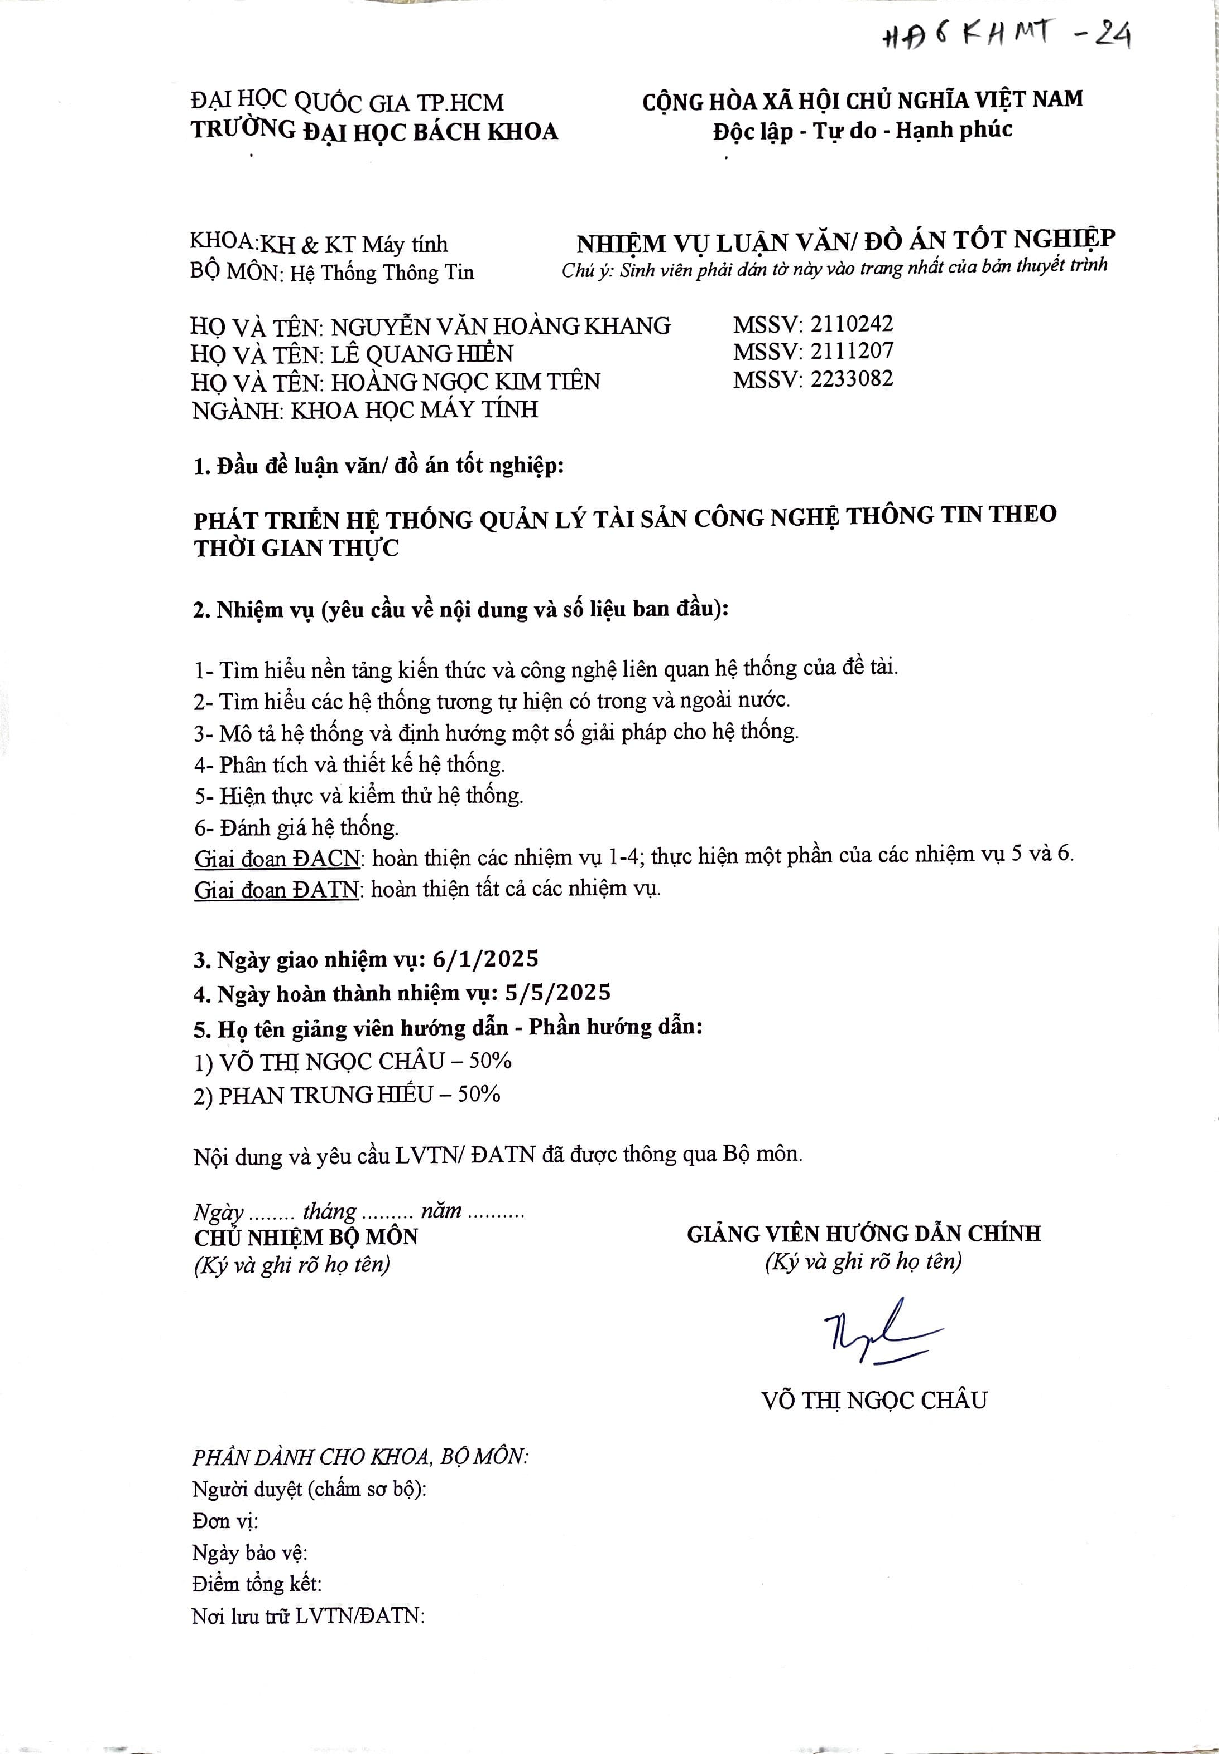
\includepdf[pages=-]{Images/Phieucham.pdf}
\newpage

\fontsize{13pt}{20pt}\selectfont

\setcounter{page}{1}

% \textbf{\large Lời cam đoan}

% Nhóm sinh viên thực hiện đề tài cam đoan mọi điều được ghi trong báo cáo, cũng như mã nguồn là do nhóm tự thực hiện - trừ các kiến thức tham khảo có trích dẫn, hoàn toàn không sao chép từ bất cứ nguồn nào khác. Nếu lời cam đoan trái với sự thật, nhóm xin chịu mọi trách nhiệm trước Ban Chủ nhiệm Khoa và Ban Giám hiệu Nhà trường.
% \vspace{0.5cm}

% \begin{flushright}
%     Nhóm sinh viên thực hiện đề tài\\
%     Nguyễn Văn Hoàng Khang, Lê Quang Hiển, Hoàng Ngọc Kim Tiên
% \end{flushright}


% \newpage
% \textbf{\large Lời cảm ơn}

% Nhóm sinh viên thực hiện đề tài xin chân thành cảm ơn quý thầy cô đã mang đến những kiến thức bổ ích trong suốt gần bốn năm học vừa qua, đặc biệt là cô Võ Thị Ngọc Châu đã tận tình giúp đỡ nhóm trong suốt quá trình thực hiện đề tài và thầy Phan Trung Hiếu đã hỗ trợ nhóm tìm hiểu kiến thức về nghiệp vụ quản lý tài sản.  

% Với điều kiện thời gian cũng như kiến thức, kinh nghiệm còn hạn chế, báo cáo Đề tài này không thể tránh khỏi những thiếu sót. Nhóm rất mong nhận được sự đóng góp, chỉ bảo của quý thầy cô để có điều kiện nâng cao kiến thức và phát triển hoàn thiện hơn trong tương lai.

% Cuối cùng, xin gửi lời cảm ơn chân thành đến các thầy cô, các anh chị và các bạn đã dành thời gian đọc bài báo cáo Đề tài này.
% \vspace{0.5cm}

% \newpage
% \textbf{\large Tóm tắt báo cáo}

% Đồ án tốt nghiệp này trình bày quá trình nghiên cứu, phân tích, thiết kế và triển khai hệ thống quản lý tài sản công nghệ thông tin (CNTT) theo thời gian thực. Trong bối cảnh nhu cầu quản lý tài sản CNTT ngày càng trở nên cấp thiết, đặc biệt là trong các tổ chức, doanh nghiệp với số lượng thiết bị lớn, việc xây dựng một hệ thống theo dõi và đánh giá tài sản theo thời gian thực mang lại nhiều lợi ích về hiệu quả và độ chính xác.

% Mở đầu báo cáo là phần giới thiệu đề tài, trong đó trình bày tổng quan về tài sản CNTT, động cơ và mục tiêu nghiên cứu, phạm vi và ý nghĩa thực tiễn của hệ thống đề xuất. Tiếp theo, đồ án tập trung tìm hiểu các công nghệ nền tảng như Python, Apache Kafka, Confluent Cloud, SQL Server, ASP.NET Core, Docker,... giúp xây dựng một hệ thống hiện đại, mở rộng và phản hồi nhanh.

% Phần tiếp theo tổng hợp và phân tích các sản phẩm tương tự đang có trên thị trường như ManageEngine, ServiceNow,... để làm cơ sở đánh giá và đề xuất hệ thống phù hợp hơn với nhu cầu thực tế tại Việt Nam. Trên cơ sở đó, báo cáo đề xuất một hệ thống quản lý tài sản CNTT bao gồm các chức năng như: theo dõi thông số tài nguyên phần cứng theo thời gian thực, cảnh báo ngưỡng sử dụng, quản lý vòng đời tài sản, và dự đoán hiệu suất sử dụng.

% Trong phần phân tích và thiết kế hệ thống, đồ án đưa ra các mô hình quy trình nghiệp vụ, mô hình hóa tương tác, thiết kế cơ sở dữ liệu và API. Đặc biệt, đề tài áp dụng mô hình học sâu LSTM để xử lý và dự đoán hiệu suất tài sản như CPU, RAM, và dùng Random Forest để dự đoán tài sản cần nâng cấp.

% Sau đó, hệ thống được hiện thực và kiểm thử trên môi trường Confluent Cloud với cấu hình Kafka, thực hiện kiểm thử các chức năng chính cũng như kiểm thử dự đoán hiệu suất sử dụng. Hệ thống được đánh giá kỹ lưỡng về hiệu năng, khả năng thu thập dữ liệu, xử lý theo thời gian thực và độ chính xác trong dự đoán thông qua các chương trình kiểm thử cụ thể.

% Cuối cùng, đồ án tiến hành triển khai hệ thống bằng Docker, thử nghiệm và cài đặt. Phần tổng kết nêu bật các kết quả đạt được, đóng góp và hạn chế còn tồn tại, đồng thời đề xuất hướng phát triển trong tương lai như tối ưu hoá mô hình dự đoán, mở rộng phạm vi thu thập dữ liệu, tăng cường bảo mật, hỗ trợ đa nền tảng, cải tiến hiệu năng và khả năng mở rộng.

% Nội dung

% \begin{flushright}
%     Nhóm sinh viên thực hiện đề tài\\
%     Nguyễn Văn Hoàng Khang, Lê Quang Hiển, Hoàng Ngọc Kim Tiên
% \end{flushright}
% \newpage
% \textbf{\large Tóm tắt}

% Đồ án tập trung vào phát triển một hệ thống quản lý tài sản công nghệ thông tin, đặc trưng bởi khả năng tự động lấy dữ liệu từ các thiết bị. Kết quả đạt được là một hệ thống quản lý tài sản vững mạnh, không chỉ thực hiện hiệu quả nhiệm vụ theo dõi và giám sát tài sản, mà còn tự động hóa quá trình thu thập dữ liệu từ các nguồn đa dạng. Sự thành công của đề tài này mang lại giá trị lớn trong việc tối ưu hóa quản lý tài sản công nghệ thông tin, đồng thời khuyến khích sự linh hoạt và nhanh nhẹn trong quá trình quản lý toàn diện.

% Trong quá trình nghiên cứu, chúng tôi không chỉ làm chủ kiến thức chuyên sâu về phát triển phần mềm mà còn áp dụng một cách linh hoạt và sáng tạo. Sự học tập trong việc quản lý tài sản công nghệ thông tin không chỉ là quá trình tiếp thu kiến thức mà còn là việc áp dụng chúng một cách hiệu quả trong môi trường thực tế. Điều này không chỉ nâng cao chuyên môn mà còn giúp chúng tôi phát triển khả năng giải quyết vấn đề và quản lý dự án.

% Đồ án không chỉ là một sản phẩm công nghệ tốt mà còn là biểu hiện của sự sáng tạo và áp dụng linh hoạt kiến thức trong hành trình nghiên cứu và học tập.
% \vspace{0.5cm}

% Nội dung

\newpage
\tableofcontents

\cleardoublepage
\addcontentsline{toc}{section}{Danh sách hình}
\listoffigures
\newpage

\cleardoublepage
\addcontentsline{toc}{section}{Danh sách bảng}
\listoftables
\newpage

% \phantomsection
% \addcontentsline{toc}{section}{Danh mục viết tắt}
% \section*{Danh mục viết tắt}

% \begin{center}
% \begin{tabular}{|c|c|c|}
%   \hline
%   \textbf{Số thứ tự} & \textbf{Ký hiệu viết tắt} & \textbf{Chữ viết đầy đủ} \\
%   \hline
%   1 & ITAM & Information Technology Asset Management \\
%   \hline 
%   2 & IT & Information Technology \\
%   \hline 
%   3 & DevOps & Development và Operations \\
%   \hline 
%   4 & SRE & Site Reliability Engineer \\
%   \hline 
%   5 & FDI & Foreign Direct Investment \\
%   \hline
%   6 & AI & Artificial Intelligence \\
%   \hline
%   7 & CNTT & Công nghệ thông tin \\
%   \hline
% \end{tabular}
% \end{center}
% \newpage

 % \subsection{Những thách thức đặt ra cho giải pháp tổng thể}
% \label{subsec:research_challenges}

% Từ những phân tích thực tiễn và tiền đề thực nghiệm nêu trên, luận văn đặt mục tiêu xây dựng một giải pháp AIOps hoàn chỉnh từ đầu đến cuối, tập trung giải quyết ba thách thức cốt lõi sau:

% \begin{enumerate}
%     \item \textbf{Hiệu chỉnh quyết định thẩm định theo nguồn gốc và nội dung bằng chứng:} Khi mở rộng đánh giá sang quy mô dữ liệu lớn với giao thức phân chia nghiêm ngặt theo từng đợt tiêm lỗi để chống rò rỉ dữ liệu, phân tích lỗi chuyên sâu cho thấy hiện tượng gia tăng đồng thời cả Recall lẫn tỷ lệ báo động giả (FPR) của truy xuất đồ thị vẫn tái diễn ($\Delta\mathrm{Recall} = +0,100$, $\Delta\mathrm{FPR} = +0,025$ trên tập tinh chỉnh)[cite: 5]. Tuy nhiên, nguyên nhân gốc rễ không phải do nhiễu từ các dịch vụ lân cận như giả định ban đầu, mà xuất phát từ \textit{thiên lệch xác nhận của LLM đối với các bằng chứng cục bộ sát thời điểm cảnh báo} (đặc biệt là các trace span có độ trễ nền vô hại)[cite: 5]. Do đó, thách thức đặt ra là thiết kế phương pháp thẩm định hiệu chỉnh (CTAV) kết hợp neo bằng chứng thực chất tại dịch vụ phát cảnh báo và ngưỡng tin cậy được hiệu chỉnh chặt chẽ, thay vì chỉ dựa vào các luật chặn cảm tính[cite: 5].
    
%     \item \textbf{Tự động hóa phân tích nguyên nhân gốc trên chuỗi cảnh báo đã thẩm định:} Một nền tảng vận hành hiệu quả không thể dừng lại ở việc phân loại từng cửa sổ cảnh báo rời rạc[cite: 4]. Hệ thống cần tích hợp một tác tử RCA tiếp nhận các cảnh báo đã được CTAV xác nhận, tự động gom cụm các cảnh báo xảy ra gần nhau thành từng sự cố thống nhất, thực hiện lan truyền ngược trên đồ thị gọi dịch vụ để xếp hạng dịch vụ nguyên nhân gốc và sinh báo cáo chẩn đoán JSON phục vụ kỹ sư SRE[cite: 4, 5].
    
%     \item \textbf{Kiểm soát ngân sách, kỷ luật đánh giá và trực quan hóa hệ thống:} Để đảm bảo tính khả thi trong môi trường sản xuất cũng như tính khách quan khoa học, toàn bộ chuỗi xử lý phải được đóng gói thành một nền tảng thống nhất có cơ chế lưu đệm (cache) định danh, tuân thủ giới hạn ngân sách gọi LLM, áp dụng quy trình đăng ký giả thuyết trước khi kiểm định độc lập trên tập kiểm thử, và cung cấp giao diện trực quan hóa theo dõi trạng thái vận hành từ lúc phát sinh cảnh báo đến khi xác định nguyên nhân gốc[cite: 1, 5].
% \end{enumerate}
\section{Giới thiệu đề tài}
\label{ch:mo-dau}
% \noindent \textit{Trong chương này, nhóm tác giả sẽ đưa ra tổng quan về đề tài, từ việc chỉ ra thực trạng quản lý tài sản công nghệ thông tin tại Việt Nam hiện nay, đến xác định rõ mục tiêu và phạm vi của đề tài mà nhóm tác giả đang thực hiện. Nhóm tác giả sẽ cung cấp một phân tích chi tiết về các yêu cầu của đề tài, làm sáng tỏ những khía cạnh quan trọng và đặc biệt trong quá trình nghiên cứu của nhóm tác giả. }
Trong các hệ thống phần mềm phân tán hiện đại xây dựng theo kiến trúc microservice, một sự cố cục bộ thường lan truyền nhanh qua nhiều services phụ thuộc và tạo ra hàng loạt cảnh báo đồng thời. Việc kết hợp các bộ Time-series Anomaly Detector với Mô hình Ngôn ngữ Lớn (LLM) mở ra khả năng tự động thẩm định cảnh báo và truy vết nguyên nhân gốc, song cũng đặt ra thách thức lớn về báo động xảy ra có là thật hay không, thiên lệch khi xác nhận và chi phí cho mỗi lần thẩm định. Đề tài này nghiên cứu và xây dựng một nền tảng AIOps, đi từ phát hiện bất thường dữ liệu metric, thẩm định cảnh báo có hiệu chỉnh theo bằng chứng đa phương thức, đến tự động hóa phân tích nguyên nhân gốc (RCA) và trực quan hóa vận hành. Chương 1 trình bày bối cảnh thực tiễn, những phát hiện thực nghiệm định hình bài toán, các mục tiêu, câu hỏi nghiên cứu, đóng góp chính, phạm vi thực hiện và bố cục tổng thể của đề tài.
\subsection{Bối cảnh và bài toán nghiên cứu}
\subsubsection{Vận hành AIOps trên hệ thống microservice và bài toán quá tải cảnh báo}
Kiến trúc microservice giúp các hệ thống đám mây đạt được tính linh hoạt, khả năng mở rộng theo chiều ngang và cô lập lỗi xảy ra tốt hơn so với kiến trúc \textit{monolithic} (nguyên khối). Tuy nhiên, khi hệ thống bị chia thành hàng chục đến hàng trăm dịch vụ độc lập, một yêu cầu từ người dùng có thể phải đi qua nhiều dịch vụ. Mỗi lần như vậy là một lần gọi qua mạng, nên luồng xử lý trở nên phức tạp hơn. Để giám sát trạng thái vận hành, các công cụ quan sát hiện đại thu thập liên tục ba nguồn dữ liệu telemetry chính: chuỗi thời gian chỉ số hiệu năng (\textit{metric}), nhật ký sự kiện bán cấu trúc (\textit{log}) và vết thực thi phân tán (\textit{trace}).

Trong thực tế vận hành, kỹ sư SRE thường dùng các công cụ tự động phát hiện bất thường trên dữ liệu metric (ví dụ thuật toán Isolation Forest~\cite{isof}) để giám sát hệ thống liên tục trên các khoảng thời gian gần nhất được cập nhật dần. Các mô hình này xử lý nhanh và tốn ít tài nguyên tính toán, nhưng vì chỉ dựa vào chuỗi số nên chúng không hiểu ngữ cảnh. Khi lưu lượng thay đổi theo chu kỳ hoặc có các tác vụ nền bình thường, chúng dễ báo động giả hàng loạt. Điều này gây \textbf{quá tải cảnh báo (alert fatigue)}~\cite{zhao2020alertstorm} và khiến đội vận hành phản ứng với sự cố chậm hơn.

Sự phát triển của các Mô hình Ngôn ngữ Lớn (LLM) giúp hệ thống có khả năng đọc hiểu và suy luận trên dữ liệu văn bản không đồng nhất như log và trace, từ đó phân biệt sự cố thật với nhiễu vận hành. Tuy vậy, khi đưa LLM vào quy trình giám sát và chẩn đoán sự cố, có ba nút thắt kỹ thuật chính:
\begin{enumerate}
    \item \textbf{Chi phí và độ trễ vận hành:} Nếu gọi LLM cho mọi khoảng dữ liệu giám sát thì chi phí API sẽ rất lớn, dễ chạm giới hạn số truy vấn và không đáp ứng được yêu cầu phản hồi nhanh của hệ thống giám sát liên tục.
    \item \textbf{Rủi ro ảo giác và thiên lệch xác nhận:} Khi thiếu ngữ cảnh vận hành phù hợp hoặc không bị buộc phải dựa trên bằng chứng cụ thể, LLM dễ suy diễn quá mức và đồng thuận theo gợi ý cảnh báo~\cite{sharma2024sycophancy}, coi những dao động vô hại là sự cố nghiêm trọng. Kết quả là báo động giả tăng lên thay vì giảm đi.
    \item \textbf{Khoảng trống từ thẩm định đến định vị nguyên nhân gốc:} Ngay cả khi từng cảnh báo riêng lẻ đã được lọc đúng, một sự cố lan rộng vẫn có thể tạo ra nhiều cảnh báo liên quan trên nhiều dịch vụ gọi nhau. Đội vận hành vẫn cần một cơ chế tự động để: gom các cảnh báo cùng thuộc một sự cố, truy ngược theo sơ đồ phụ thuộc giữa các dịch vụ để tìm đúng thành phần khởi phát sự cố (RCA), và tổng hợp thành báo cáo chẩn đoán có cấu trúc.
\end{enumerate}

\begin{figure}[H]
    \centering
     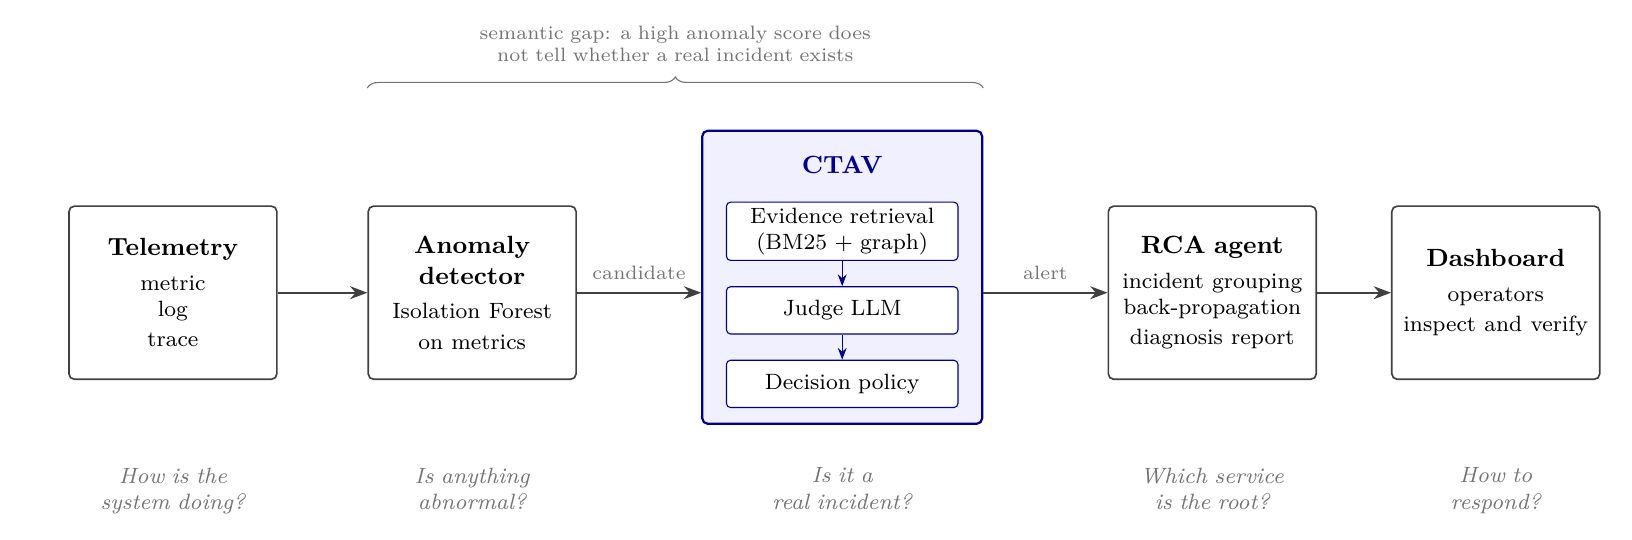
\includegraphics[width=0.88\textwidth]{Images/C1/figures/ch1/h1.1-system-overview.png}
    % \fbox{\parbox{0.85\textwidth}{\centering\vspace{1.2cm}\textit{Hình 1.1: Khoảng trống ngữ nghĩa của bộ phát hiện metric và quy trình từ thẩm định cảnh báo đến chẩn đoán nguyên nhân gốc]}}
    \vspace{0.5cm}
    \caption{Tổng quan hệ thống}
    \label{fig:ch1_alert_fatigue}
\end{figure}
\subsubsection{Khảo sát bước đầu về kiến trúc giám sát lai và đánh đổi ngữ cảnh đồ thị}  
Để giải quyết bài toán chi phí và khoảng trống ngữ nghĩa, hướng tiếp cận kiến trúc giám sát lai hai tầng được thiết lập: \textbf{tầng thứ nhất} sử dụng bộ phát hiện metric tốc độ cao để sàng lọc các cửa sổ đáng nghi thành danh sách cảnh báo ứng viên; \textbf{tầng thứ hai} kết hợp kỹ thuật RAG~\cite{lewis2020rag} trên dữ liệu log/trace với một LLM đóng vai trò bộ thẩm định (\textit{LLM-as-a-Judge})~\cite{zheng2023judging} xuất kết quả theo lược đồ JSON ràng buộc.

Trong quá trình khảo sát bước đầu tầng truy xuất bằng chứng trên bộ dữ liệu microservice Nezha~\cite{icaetm2026}, việc đối chiếu giữa truy xuất từ khóa truyền thống (BM25)~\cite{robertson2009bm25} và truy xuất mở rộng theo đồ thị gọi dịch vụ 2-hop (mở rộng \textit{2-hop} nghĩa là thu thập thêm bằng chứng log và trace từ các dịch vụ nằm cách dịch vụ phát cảnh báo tối đa hai bước liên kết trên đồ thị phụ thuộc (tính theo cả hai chiều gọi đến và được gọi)) đã bộc lộ một nghịch lý đáng chú ý trong thiết kế hệ thống giám sát lai (minh họa ở Hình~\ref{fig:ch1_alert_fatigue}):
\begin{itemize}
    \item \textbf{Lợi ích trong việc phát hiện sự cố lan truyền:} Nhiều sự cố hạ tầng (chẳng hạn độ trễ mạng) không sinh ra thông báo lỗi tường minh ngay tại dịch vụ phát cảnh báo, khiến truy xuất từ khóa cục bộ dễ bỏ sót do thiếu ngữ cảnh. Khi mở rộng phạm vi tìm kiếm sang các dịch vụ lân cận trên đồ thị phụ thuộc, hệ thống thu thập được chuỗi dấu vết liên đới giữa các dịch vụ gọi nhau, từ đó cải thiện rõ rệt khả năng nhận diện các sự cố lan truyền phức tạp.
    \item \textbf{Rủi ro bùng nổ báo động giả do thiếu hiệu chỉnh:} Trong trạng thái vận hành bình thường, truy xuất từ khóa thường trả về ngữ cảnh rỗng vì không có từ khóa lỗi, vô tình đóng vai trò như một lớp lọc nhiễu tự nhiên giúp bộ thẩm định LLM bác bỏ cảnh báo. Ngược lại, việc mở rộng ngữ cảnh theo đồ thị lại nạp thêm nhiều tín hiệu cảnh báo nền vô hại từ các dịch vụ xung quanh, dễ kích hoạt thiên lệch xác nhận ở LLM, làm gia tăng đột biến báo động giả và đẩy chi phí gọi API lên cao.
\end{itemize}
Phát hiện thực nghiệm này cho thấy truy xuất đồ thị và bộ thẩm định LLM không thể được thiết kế như hai mô-đun tách rời. Tuy nhiên, việc chỉ dừng lại ở nhận diện hiện tượng đánh đổi trên một tập mẫu cố định vẫn chưa giải quyết được toàn bộ bài toán vận hành thực tế.
\subsubsection{Những thách thức đặt ra cho giải pháp tổng thể}

Từ những phân tích thực tiễn và tiền đề thực nghiệm nêu trên, đề tài hướng tới xây dựng một giải pháp AIOps hoàn chỉnh từ đầu đến cuối, tập trung giải quyết ba thách thức cốt lõi sau:

\begin{enumerate}
    \item \textbf{Hiệu chỉnh quyết định thẩm định theo nguồn gốc và nội dung bằng chứng:} Khi mở rộng đánh giá sang quy mô dữ liệu lớn với quy trình phân chia chống rò rỉ dữ liệu theo từng đợt tiêm lỗi, phân tích chuyên sâu cho thấy hiện tượng gia tăng đồng thời cả khả năng phát hiện sự cố lẫn báo động giả của truy xuất đồ thị vẫn tái diễn. Tuy nhiên, nguyên nhân gốc rễ không phải do nhiễu từ các dịch vụ lân cận như giả định ban đầu, mà xuất phát từ \textit{thiên lệch xác nhận của LLM đối với các bằng chứng cục bộ sát thời điểm cảnh báo} (ngay cả khi đó chỉ là các dấu vết thực thi nền vô hại). Do đó, thách thức đặt ra là thiết kế phương pháp thẩm định hiệu chỉnh (CTAV) kết hợp cơ chế neo bằng chứng thực chất tại dịch vụ phát cảnh báo và ngưỡng tin cậy được hiệu chỉnh chặt chẽ, thay vì chỉ dựa vào các luật chặn cảm tính.
    
    \item \textbf{Tự động hóa phân tích nguyên nhân gốc trên chuỗi cảnh báo đã thẩm định:} Một nền tảng vận hành hiệu quả không thể dừng lại ở việc phân loại từng cửa sổ cảnh báo rời rạc. Hệ thống cần tích hợp một tác tử RCA tiếp nhận các cảnh báo đã được CTAV xác nhận, tự động gom cụm các cảnh báo liên quan thành từng sự cố thống nhất, thực hiện lan truyền ngược trên đồ thị gọi dịch vụ để xếp hạng dịch vụ khởi phát và sinh báo cáo chẩn đoán có cấu trúc phục vụ kỹ sư vận hành.
    
    \item \textbf{Kiểm soát ngân sách, kỷ luật đánh giá và trực quan hóa vận hành:} Để đảm bảo tính khả thi trong thực tế cũng như tính khách quan khoa học, toàn bộ chuỗi xử lý cần được đóng gói thành một nền tảng thống nhất. Hệ thống phải có cơ chế lưu đệm định danh nhằm tiết kiệm chi phí và tuân thủ giới hạn ngân sách gọi LLM, áp dụng kỷ luật kiểm định giả thuyết nghiêm ngặt trên tập dữ liệu độc lập, đồng thời cung cấp giao diện trực quan hóa xuyên suốt từ lúc phát sinh cảnh báo đến khi khoanh vùng nguyên nhân gốc.
\end{enumerate}

\subsection{Mục tiêu đề tài}
\subsubsection{Mục tiêu tổng quát}
Mục tiêu tổng quát của đề tài là nghiên cứu, đề xuất và kiểm chứng một giải pháp AIOps khép kín trên hệ thống microservice gồm ba khối liên kết chặt chẽ: phương pháp thẩm định cảnh báo hiệu chỉnh theo bằng chứng đa phương thức (\CTAV{}) nhằm giữ khả năng phát hiện sự cố lan truyền mà không làm tăng báo động giả trong cùng ngân sách gọi LLM; tác tử phân tích nguyên nhân gốc (RCA) gom các cảnh báo đã xác nhận, truy ngược đồ thị phụ thuộc để định vị dịch vụ khởi phát và sinh báo cáo chẩn đoán có cấu trúc; cùng nền tảng thực nghiệm thống nhất có bộ nhớ đệm định danh và giao diện trực quan hóa tái lập được.
\subsubsection{Mục tiêu cụ thể}
Để đạt các mục tiêu tổng quát trên, đề tài thực hiện năm mục tiêu cụ thể:
\begin{itemize}[label=--]
    \item \textbf{Xây dựng giao thức đánh giá chống rò rỉ và xác lập bài toán:}
    chia dữ liệu Nezha theo từng đợt tiêm lỗi, có vùng đệm thời gian giữa các split;
    trên giao thức đó, kiểm chứng rằng mở rộng ngữ cảnh theo topology làm tăng recall
    nhưng cũng làm tăng báo động giả so với truy xuất BM25.

    \item \textbf{Phân tích cơ chế báo động giả của judge LLM:}
    can thiệp có kiểm soát vào ngữ cảnh truy xuất (độ gần thời gian, loại bằng chứng,
    thứ tự trình bày) để xác định yếu tố khiến thẩm định xác nhận nhầm cửa sổ bình thường.

    \item \textbf{Đề xuất phương pháp CTAV:}
    kết hợp truy xuất hybrid BM25--topology, ngưỡng tin cậy cho quyết định của judge
    và cơ chế neo bằng chứng, chỉ chấp nhận cảnh báo khi chính service phát cảnh báo
    có tín hiệu bất thường.

    \item \textbf{Kiểm định theo giả thuyết đăng ký trước:}
    đánh giá một lần trên split \texttt{test} niêm phong bằng bootstrap CI~\cite{efron1993bootstrap} và McNemar~\cite{mcnemar1947note},
    gồm so sánh với các baseline, \textit{ablation} từng thành phần
    và hiệu quả theo ngân sách gọi LLM.

    \item \textbf{Xây dựng tác tử RCA và platform end-to-end:}
    gom cảnh báo đã thẩm định thành sự cố, lan truyền ngược trên đồ thị phụ thuộc
    để xếp hạng service gốc và sinh báo cáo chẩn đoán có cấu trúc; tích hợp toàn bộ
    pipeline với dashboard thành một platform chạy được và tái lập được từ \textit{cache}.
\end{itemize}
\subsection{Đối tượng và phạm vi nghiên cứu}
\label{subsec:scope}

\subsubsection{Đối tượng nghiên cứu}
\label{subsubsec:research_objects}

Đề tài tập trung vào ba đối tượng trong chuỗi giám sát và chẩn đoán sự cố tự động trên microservice:
\begin{itemize}[label=--]
    \item \textbf{Dữ liệu quan sát đa phương thức và đồ thị phụ thuộc:} cửa sổ metric, log, trace và đồ thị gọi dịch vụ dựng từ trace.
    \item \textbf{Phương pháp thẩm định cảnh báo \CTAV{}:} truy xuất lai theo từ vựng--topology, bộ thẩm định LLM có cấu trúc và chính sách neo bằng chứng tại dịch vụ phát cảnh báo.
    \item \textbf{Tác tử RCA và nền tảng thực nghiệm:} gom cụm sự cố, lan truyền ngược xếp hạng dịch vụ gốc, báo cáo chẩn đoán JSON và dashboard trực quan hóa.
\end{itemize}

\subsubsection{Phạm vi nghiên cứu}
\label{subsubsec:research_scope}

Phạm vi của đề tài được giới hạn ở ba khía cạnh:
\begin{itemize}[label=--]
    \item \textbf{Dữ liệu và môi trường:} một bộ dữ liệu công khai là Nezha~\cite{nezha}, thu từ hai hệ microservice
mẫu (OnlineBoutique, TrainTicket) với các loại lỗi tiêm có chủ đích (độ trễ mạng, tranh chấp và
tiêu thụ CPU, ngoại lệ, giá trị trả về sai). Dữ liệu được chia theo từng đợt tiêm lỗi để chống
rò rỉ; chỉ số chính tính trên các cửa sổ có telemetry. Hệ thống chạy bằng cách phát lại dữ liệu
và đọc lại từ \textit{cache}, không triển khai trên hạ tầng production và chưa kiểm chứng trên
bộ dữ liệu khác.

    \item \textbf{Mô hình:} bộ phát hiện bất thường cố định là Isolation Forest. Judge và bộ tóm tắt
    sự cố dùng một LLM duy nhất qua API (\texttt{gemini-2.5-flash}~\cite{google2026gemini}, temperature 0); đề tài không
    fine-tuning và không dùng LLM cục bộ.

    \item \textbf{Đánh giá:} chất lượng thẩm định cảnh báo (Precision, Recall, F1, FPR), định vị
    dịch vụ gốc (Hit@$k$, tỷ lệ giảm cảnh báo), chi phí gọi LLM theo ngân sách, và độ ổn định
    của judge khi gọi lặp lại. Mọi so sánh giữa các phương pháp đều kèm khoảng tin cậy bootstrap
    và kiểm định McNemar.
\end{itemize}

\subsection{Ý nghĩa của đề tài}
\label{subsec:significance}

\subsubsection{Ý nghĩa thực tiễn}
\label{subsubsec:practical_significance}

Trên hệ thống microservice, bộ phát hiện bất thường dựa trên metric sinh ra nhiều cảnh báo, phần lớn không ứng với sự cố thật. Mỗi cảnh báo sai lấy đi thời gian của đội vận hành và làm giảm niềm tin vào hệ thống giám sát. Đề tài đặt một judge LLM sau bộ phát hiện để đọc bằng chứng log và trace trước khi xác nhận cảnh báo. Kết quả thực nghiệm cho thấy cung cấp thêm ngữ cảnh không tự động làm quyết định tốt hơn: ngữ cảnh theo topology giúp bắt thêm sự cố nhưng cũng kéo theo báo động giả. Vì vậy, khi triển khai cần một chính sách quyết định kiểm soát được nguồn gốc của bằng chứng, chứ không chỉ một bộ truy xuất tốt hơn.

Đề tài đo hiệu quả theo số lần gọi LLM, nhờ đó đội vận hành có thể ước lượng chi phí trước khi
triển khai. Tác tử RCA nối tiếp quá trình này: gom các cảnh báo đã thẩm định thành sự cố, chỉ ra dịch vụ gốc và sinh báo cáo chẩn đoán có cấu trúc, rút ngắn bước chẩn đoán thủ công. Toàn bộ chuỗi xử lý chạy trên một platform tái lập được từ \textit{cache}, có thể dùng làm môi trường thử chính sách thẩm định trước khi áp dụng lên hệ thống thật. Các kết quả này thu được trên dữ liệu phát lại của Nezha; áp dụng cho hệ thống production cần được kiểm chứng thêm.

\subsubsection{Ý nghĩa khoa học}
\label{subsubsec:scientific_significance}

Về mặt khoa học, đề tài làm rõ vì sao ngữ cảnh topology làm tăng báo động giả của judge LLM.
Giả thuyết ban đầu cho rằng bằng chứng từ các dịch vụ lân cận gây nhiễu, nhưng thực nghiệm có kiểm soát không ủng hộ giả thuyết này. Nguyên nhân phù hợp hơn là thiên lệch xác nhận: judge dễ xác nhận cảnh báo khi gặp bằng chứng cục bộ nằm sát thời điểm cảnh báo, nhất là bằng chứng từ trace. Phát hiện này chuyển trọng tâm từ câu hỏi ``truy xuất gì'' sang câu hỏi ``quyết định thế nào với bằng chứng đã truy xuất'', và là cơ sở thiết kế phương pháp CTAV.

Đề tài cũng đóng góp về phương pháp luận cho việc đánh giá LLM trong AIOps. Dữ liệu được chia theo từng đợt tiêm lỗi để chống rò rỉ; giả thuyết và tiêu chí bác bỏ được đăng ký trước khi tiếp cận tập kiểm thử; mọi so sánh đều kèm khoảng tin cậy bootstrap và kiểm định McNemar thay vì một điểm số đơn lẻ. Các thiết kế không đạt kỳ vọng, như ngưỡng riêng theo nguồn bằng chứng, định tuyến hai tầng và cơ chế cứu cảnh báo, được báo cáo cùng bằng chứng loại bỏ. Những kết quả âm này giúp các nghiên cứu sau tránh lặp lại các thiết kế đã được kiểm chứng là không hiệu quả.
% \subsection{Cấu trúc báo cáo}
% % \subsection{Cấu trúc báo cáo}
% \noindent Báo cáo \textbf{Thực tập 1} này gồm 7 chương, với các nội dung chính được trình
% bày trong bảng sau:
% \begin{longtable}{|>{\centering\arraybackslash}m{2cm}|>{\centering\arraybackslash}m{10cm}|}
%     \caption{Cấu trúc báo cáo Đồ án Chuyên ngành} \\
%     \hline
%     \textbf{Chương} & \textbf{Nội dung} \\
%     \hline
%     \endfirsthead

%     \hline
%     \textbf{Chương} & \textbf{Nội dung} \\
%     \hline
%     \endhead 
%     1 & Giới thiệu tổng quan đề tài\\  
%     \hline 
%     2 & Kiến thức và công nghệ nền tảng \\  
%     \hline 
%     3 & Các công trình liên quan \\  
%     \hline 

%     4 & Hệ thống đề xuất\\  
%     \hline 

%     5 & Phân tích và thiết kế \\  
%     \hline 
%     6 & Hiện thực và kiểm thử \\  
%     \hline 
%     7 & Triển khai hệ thống\\  
%     \hline 
%     8 & Đánh giá hệ thống \\  
%     \hline 
%     9 & Tổng kết \\  
%     \hline 
    
    
% \end{longtable}
 \newpage
 % =============================================================================
% Chuong 2: Kien thuc va cong nghe nen tang
% =============================================================================
% Cach dung tren Overleaf:
%   1. Tai thu muc thesis/ (hoac sao chep macros.tex, refs.bib, chapters/ch2.tex
%      va figures/ch2/*.png) vao du an Overleaf.
%   2. Trong main.tex:
%        \input{macros}
%        ...
%        \include{chapters/ch2}
%        ...
%        \bibliographystyle{IEEEtran}
%        \bibliography{refs}
%
% Cac nhan lien chuong duoc tham chieu tu Chuong 2 (dat dung \label o cac
% chuong tuong ung de \ref tu dong hien so):
%   Chuong: ch:de-xuat, ch:thuc-nghiem, ch:platform, ch:thao-luan
%   Chuong 4: sec:ch4-detector, sec:ch4-ctav, sec:ch4-bm25, sec:ch4-c1,
%             sec:ch4-policy, sec:ch4-c4, sec:ch4-judge, sec:ch4-rca,
%             sec:ch4-grouping, sec:ch4-propagation, sec:ch4-report, sec:ch4-impl
%   Chuong 5: sec:ch5-hypotheses, sec:ch5-data, sec:ch5-metrics, sec:ch5-val,
%             sec:ch5-h1, sec:ch5-c5, sec:ch5-h4, sec:ch5-budget, sec:ch5-rca,
%             tab:h0-h5
%   Chuong 7: sec:ch7-threats
% =============================================================================

\section{Kiến thức và công nghệ nền tảng}
\label{ch:nen-tang}

Chương này trình bày các khái niệm và công nghệ mà phần đề xuất (Chương~\ref{ch:de-xuat}) và phần thực nghiệm (Chương~\ref{ch:thuc-nghiem}) dựa vào. Nội dung đi theo đúng thứ tự xử lý của hệ thống. Mục~\ref{sec:ch2-du-lieu} mô tả dữ liệu quan sát của hệ microservice và bộ dữ liệu Nezha. Mục~\ref{sec:ch2-phat-hien} nói về phát hiện bất thường và hiện tượng quá tải cảnh báo. Mục~\ref{sec:ch2-truy-xuat} trình bày các cách truy xuất bằng chứng từ log và trace: \term{BM25}{BM25}, đồ thị phụ thuộc service và cách hợp nhất chúng. Mục~\ref{sec:ch2-judge} giải thích cơ chế dùng mô hình ngôn ngữ lớn làm bộ thẩm định và các rủi ro của nó, Mục~\ref{sec:ch2-rca} giới thiệu bài toán phân tích nguyên nhân gốc. Mục~\ref{sec:ch2-danh-gia} và Mục~\ref{sec:ch2-dang-ky} định nghĩa chỉ số, kiểm định thống kê và nguyên tắc đăng ký giả thuyết trước. Mục~\ref{sec:ch2-cong-nghe} giới thiệu các công nghệ dùng để hiện thực hệ thống, và Mục~\ref{sec:ch2-ket-chuong} tổng kết.

% -----------------------------------------------------------------------------
\subsection{Dữ liệu quan sát trên hệ microservice}
\label{sec:ch2-du-lieu}

Mục này xác định đơn vị dữ liệu mà toàn bộ đề tài làm việc trên đó: ba loại tín hiệu quan sát, cách cắt chúng thành cửa sổ, và bộ dữ liệu có nhãn dùng để đánh giá.

\subsubsection{Metric, log, trace và cửa sổ trượt}
\label{sec:ch2-tin-hieu}

Một hệ microservice gồm nhiều service nhỏ, mỗi service chạy trên một hoặc nhiều pod và gọi nhau qua mạng. Khả năng quan sát (\emph{observability}) của hệ dựa trên ba loại tín hiệu, tóm tắt ở Bảng~\ref{tab:ch2-tin-hieu}. \textbf{Metric} là chuỗi thời gian số đo định kỳ cho từng pod, như mức dùng CPU, bộ nhớ, lưu lượng mạng hay độ trễ phân vị. Độ trễ phân vị P$k$ là mức độ trễ mà $k\%$ request trong chu kỳ đo không vượt quá: P99 bằng $500$~ms nghĩa là $99\%$ request hoàn tất trong $500$~ms, nên P95 và P99 phản ánh phần đuôi chậm mà độ trễ trung bình che mất. Khái niệm phân vị này cũng là cơ sở của ngưỡng nền $p_{90}$ mà cơ chế neo bằng chứng \comp{C3} dùng (Mục~\ref{sec:ch4-policy}). \textbf{Log} là các dòng văn bản do service ghi ra, thường kèm mức nghiêm trọng (\code{INFO}, \code{WARN}, \code{ERROR}). \textbf{Trace} ghi lại đường đi của một request qua nhiều service. Mỗi bước trên đường đi là một \textbf{span}, có định danh \code{SpanID}, định danh span cha \code{ParentID}, tên thao tác và thời lượng. Quan hệ cha--con giữa các span cho biết service nào gọi service nào.

\begin{table}[H]
  \centering
  \caption{Ba loại tín hiệu quan sát trên Nezha và vai trò của chúng trong đề tài.}
  \label{tab:ch2-tin-hieu}
  \tblfont
  \tblsetup
  \renewcommand{\arraystretch}{1.35}
  \setlength{\tabcolsep}{6pt}
  \begin{tabularx}{\linewidth}{|l|>{\hsize=0.70\hsize}Y|>{\hsize=1.45\hsize}Y|>{\hsize=0.85\hsize}Y|}
    \hline
    \rowcolor{gray!15}
    \textbf{Tín hiệu} & \textbf{Dạng dữ liệu trên Nezha} & \textbf{Trường chính} & \textbf{Vai trò trong đề tài} \\
    \hline
    Metric & CSV theo pod, một mẫu mỗi 60~s & 19 chỉ số: CPU, bộ nhớ, syscall, mạng vào/ra, độ trễ client/server ở phân vị 90/95/99 (P90/P95/P99), workload, tỉ lệ thành công, tài nguyên node & Đầu vào của bộ phát hiện bất thường \\
    \hline
    Log & CSV theo phút & thời điểm, pod, \code{TraceID}, \code{SpanID}, nội dung (kèm mức nghiêm trọng) & Bằng chứng văn bản cho judge \\
    \hline
    Trace & CSV theo phút & \code{TraceID}, \code{SpanID}, \code{ParentID}, pod, tên thao tác, thời điểm bắt đầu/kết thúc, thời lượng & Bằng chứng về độ trễ; nguồn dựng đồ thị phụ thuộc service \\
    \hline
  \end{tabularx}
\end{table}


Đề tài dùng metric để \emph{phát hiện} và dùng log, trace làm \emph{bằng chứng}. Cách chia vai này bám theo cách dữ liệu được ghi: metric có ở mọi thời điểm, còn log và trace dày đặc và cần được chọn lọc trước khi đưa cho một mô hình đọc.

\textbf{Cửa sổ. (Window)} Đơn vị phân tích của hệ là \textbf{cửa sổ}: một mẫu metric của một pod dài $60\,\text{s}$ (chu kỳ lấy mẫu của Nezha), có định danh tất định từ service, pod và thời điểm bắt đầu. Một cửa sổ được gán nhãn \textbf{có sự cố} nếu thuộc đúng pod bị tiêm lỗi và rơi vào khoảng $[t_{\mathrm{inject}} - 60\text{ s},\; t_{\mathrm{inject}} + 360\text{ s}]$ (khoảng bảy cửa sổ mỗi lần tiêm, bắt cả dấu hiệu sớm lẫn thời gian lỗi lan); các cửa sổ còn lại là bình thường. Bộ phát hiện không nhìn cửa sổ cô lập mà duy trì bộ đệm trượt ngắn trên cùng pod (Mục~\ref{sec:ch4-detector}), còn bằng chứng log/trace được tìm trong biên $\pm 8$~phút quanh cửa sổ. Định nghĩa cửa sổ và quy tắc nhãn này được dùng thống nhất cho bộ phát hiện ở Chương~\ref{ch:de-xuat} và mọi phép đo ở Chương~\ref{ch:thuc-nghiem}.

\subsubsection{Nezha và nhãn nguyên nhân gốc}
\label{sec:ch2-nezha}

Nezha~\cite{nezha} là bộ dữ liệu quan sát đa phương thức (metric, log, trace) thu từ hai hệ microservice mẫu là \textbf{OnlineBoutique} và \textbf{TrainTicket}, với các lỗi được tiêm có chủ đích (độ trễ mạng, tranh chấp/tiêu thụ CPU, ngoại lệ, giá trị trả về sai). Đề tài dùng bốn ngày dữ liệu gồm $101$ lần tiêm lỗi trên $95.660$ cửa sổ thuộc $103$ pod ($56$ service), trong đó chỉ có $704$ cửa sổ có sự cố ($\approx 0{,}74\%$, tỷ lệ mất cân bằng xấp xỉ $1:135$). Mỗi lần tiêm lỗi ghi rõ pod bị tiêm và ánh xạ được về tên \textbf{service gốc} cho bài toán \term{RCA}{RCA} (Mục~\ref{sec:ch2-hitk}); đề tài sử dụng cột giờ hệ thống (\emph{wall-clock}) nhất quán trên cả bốn ngày.

Để tránh rò rỉ dữ liệu theo sự kiện và thời gian, dữ liệu được chia thành ba tập \splitname{dev}, \splitname{val} và \splitname{test} theo đơn vị \textbf{lần tiêm lỗi} kèm \textbf{vùng đệm $600\,\text{s}$}, giữ nguyên tỷ lệ mất cân bằng tự nhiên. Do Nezha chỉ ghi log và trace quanh các khoảng tiêm lỗi (chỉ khoảng một phần tư cửa sổ bình thường có telemetry), chỉ số chính của nhánh thẩm định được tính trên tập con \textbf{\term{TelemetryWindow}{cửa sổ có telemetry}} (xác định chỉ từ danh sách tệp, không dùng nhãn) nhằm tránh việc bộ thẩm định bác bỏ đúng một cách tầm thường trên vùng trống dữ liệu. Chi tiết kích thước từng split, độ phủ telemetry và rủi ro tính hợp lệ liên quan được trình bày ở Mục~\ref{sec:ch5-data} và Mục~\ref{sec:ch7-hop-le}.

% -----------------------------------------------------------------------------
\subsection{Phát hiện bất thường và quá tải cảnh báo}
\label{sec:ch2-phat-hien}

Mục này giải thích vì sao một bộ phát hiện bất thường trên metric chưa đủ để cảnh báo người vận hành, và giới thiệu Isolation Forest, bộ phát hiện mà đề tài sử dụng.

\subsubsection{Bất thường, khoảng trống ngữ nghĩa và quá tải cảnh báo}
\label{sec:ch2-khoang-trong}

\textbf{Bất thường} (\emph{anomaly}) là điểm dữ liệu lệch khỏi hành vi thường gặp của hệ. Một bộ phát hiện bất thường gán cho mỗi cửa sổ một \textbf{điểm bất thường} và so với một ngưỡng; cửa sổ vượt ngưỡng trở thành \textbf{candidate} cảnh báo. Điểm này chỉ nói rằng số đo khác thường. Nó không nói số đo khác thường \emph{vì sao}, cũng không nói có sự cố hay không. Một đợt tải tăng hợp lệ, một tác vụ định kỳ hay một pod vừa khởi động lại đều có thể làm metric lệch. Khoảng cách giữa ``số đo lệch'' và ``có sự cố cần người xử lý'' được gọi là \textbf{khoảng trống ngữ nghĩa}. Để lấp khoảng trống này, cần ngữ cảnh vận hành mà metric không có, chẳng hạn log lỗi hay trace chậm.

Khi khoảng trống không được lấp, người vận hành nhận rất nhiều cảnh báo, phần lớn là báo động giả. Hiện tượng này gọi là \textbf{quá tải cảnh báo} (\emph{alert fatigue}): người vận hành dần bỏ qua cảnh báo, kể cả cảnh báo thật~\cite{zhao2020alertstorm}. Trên Nezha, mất cân bằng $1:135$ cho thấy vấn đề rõ ràng. Giả sử một bộ phát hiện chỉ báo nhầm 1\% cửa sổ bình thường của \splitname{val} (28.689 cửa sổ). Nó đã sinh khoảng 287 báo động giả, nhiều hơn cả tổng số cửa sổ có sự cố của split này (209). Precision khi đó không thể vượt $209 / (209 + 287) \approx 0{,}42$, kể cả khi bộ phát hiện bắt trọn mọi sự cố.

Đề tài không thay bộ phát hiện. Đề tài thêm một khâu \textbf{thẩm định cảnh báo} đứng sau nó: mỗi candidate được đối chiếu với bằng chứng từ log và trace trước khi chuyển cho người vận hành. Khâu này là \CTAV{} (thẩm định cảnh báo hiệu chỉnh theo bằng chứng đa phương thức), trình bày ở Mục~\ref{sec:ch4-ctav}.

\subsubsection{Isolation Forest}
\label{sec:ch2-iforest}

Isolation Forest~\cite{isof} phát hiện bất thường bằng cách \emph{cô lập} điểm dữ liệu thay vì mô hình hoá dữ liệu bình thường. Ý tưởng là: điểm bất thường ít và khác biệt, nên dễ bị tách riêng bằng vài nhát cắt ngẫu nhiên. Thuật toán dựng nhiều cây cô lập. Mỗi cây chọn ngẫu nhiên một đặc trưng và một giá trị cắt nằm giữa giá trị nhỏ nhất và lớn nhất của đặc trưng đó, rồi chia đệ quy cho đến khi mỗi điểm nằm riêng một lá. Độ dài đường đi $h(x)$ từ gốc tới lá chứa điểm $x$ càng ngắn thì $x$ càng dễ cô lập, tức càng bất thường. Điểm bất thường chuẩn hoá của $x$ trên tập huấn luyện cỡ $n$ được định nghĩa ở Phương trình~\eqref{eq:ch2-iforest}:
\begin{align}
  s(x, n) &= 2^{-\mathbb{E}[h(x)] / c(n)}, \nonumber \\
  c(n) &= 2 H(n - 1) - \frac{2(n - 1)}{n}, \qquad H(i) \approx \ln(i) + 0{,}5772,
  \label{eq:ch2-iforest}
\end{align}
trong đó $\mathbb{E}[h(x)]$ là độ dài đường đi trung bình qua các cây và $c(n)$ là độ dài đường đi trung bình của một tìm kiếm không thành công trên cây nhị phân, dùng để chuẩn hoá. Giá trị $s$ gần 1 nghĩa là rất bất thường; $s$ quanh 0,5 hoặc thấp hơn nghĩa là bình thường. Thuật toán không cần nhãn, chạy nhanh và ít tham số. Đó là lý do nó hợp với vai trò bộ lọc đầu tiên trên luồng metric lớn.

Đề tài fit Isolation Forest trên \splitname{dev} không dùng nhãn, sử dụng các thống kê trên bộ đệm trượt của từng pod, rồi quy điểm $s(x, n)$ về \textbf{thứ hạng phân vị} trên tập huấn luyện để ngưỡng trở nên dễ diễn giải và độc lập thang đo thô (ví dụ ngưỡng $0{,}85$ nghĩa là bất thường hơn $85\%$ cửa sổ \splitname{dev}). Chi tiết bộ đệm, xử lý giá trị thiếu và cổng Rescue cho cửa sổ dưới ngưỡng được trình bày ở Mục~\ref{sec:ch4-detector}.

% -----------------------------------------------------------------------------
\subsection{Truy xuất bằng chứng}
\label{sec:ch2-truy-xuat}

Mục này trình bày cách chọn một số ít sự kiện log và trace làm bằng chứng cho một candidate: truy xuất theo từ vựng (\term{BM25}{BM25}), theo đồ thị phụ thuộc service, cách hợp nhất các tín hiệu đó, và khung chung \term{RAG}{RAG}.

\subsubsection{\term{BM25}{BM25} trên văn bản log và trace}
\label{sec:ch2-bm25}

\textbf{\term{BM25}{BM25}}~\cite{robertson2009bm25} là hàm xếp hạng tài liệu theo mức khớp từ vựng với truy vấn. Mỗi sự kiện log hoặc span được coi là một tài liệu văn bản đã tách thành từ. Với truy vấn $Q = \{q_1, \dots, q_m\}$ và tài liệu $D$, điểm \term{BM25}{BM25} được tính theo Phương trình~\eqref{eq:ch2-bm25}:
\begin{align}
  \mathrm{BM25}(D, Q) &= \sum_{i=1}^{m} \mathrm{IDF}(q_i) \cdot
    \frac{f(q_i, D) \cdot (k_1 + 1)}{f(q_i, D) + k_1 \cdot \left(1 - b + b \cdot \dfrac{|D|}{\mathrm{avgdl}}\right)}, \nonumber \\
  \mathrm{IDF}(q) &= \ln\!\left(1 + \frac{N - n(q) + 0{,}5}{n(q) + 0{,}5}\right),
  \label{eq:ch2-bm25}
\end{align}
trong đó $f(q, D)$ là số lần từ $q$ xuất hiện trong $D$, $|D|$ là độ dài tài liệu, $\mathrm{avgdl}$ là độ dài trung bình của kho, $N$ là số tài liệu và $n(q)$ là số tài liệu chứa $q$. Tham số $k_1$ điều khiển mức bão hoà theo tần suất từ, còn $b$ điều khiển mức phạt tài liệu dài. Đề tài dùng $k_1 = 1{,}5$ và $b = 0{,}75$. Từ hiếm (IDF cao) như tên một service hay một mã lỗi đóng góp nhiều hơn từ phổ biến như ``request''.

\textbf{Truy vấn sinh từ candidate} ghép tên service, tên pod và các metric lệch nhiều nhất, tuyệt đối \textbf{không} đưa loại lỗi đã tiêm (nhãn) vào truy vấn để chống rò nhãn; bằng chứng chỉ tìm trong biên $\pm 8$~phút quanh cửa sổ. \term{BM25}{BM25} không cần huấn luyện và là nền tảng của baseline \code{bm25\_hybrid} ở Mục~\ref{sec:ch4-bm25}.

\subsubsection{Đồ thị phụ thuộc service}
\label{sec:ch2-do-thi}

\textbf{Đồ thị phụ thuộc service} $G = (V, A)$ biểu diễn mỗi service là một nút và có cạnh có hướng $u \to v$ khi span của $u$ là cha của span thuộc $v$ trong trace ($u$ gọi $v$). Dựng từ $307$ tệp trace của Nezha ($\approx 4{,}18$ triệu span, lọc cạnh xuất hiện $< 5$ lần), đồ thị có $56$ service và $68$ cạnh (Hình~\ref{fig:ch2-service-graph}), gồm $20$ thành phần liên thông (thành phần lớn nhất $28$ service, $18$ service TrainTicket cô lập). Khoảng cách vô hướng $d_G(s, s')$ là số cạnh ngắn nhất giữa hai service.

\begin{figure}[htbp]
  \centering
  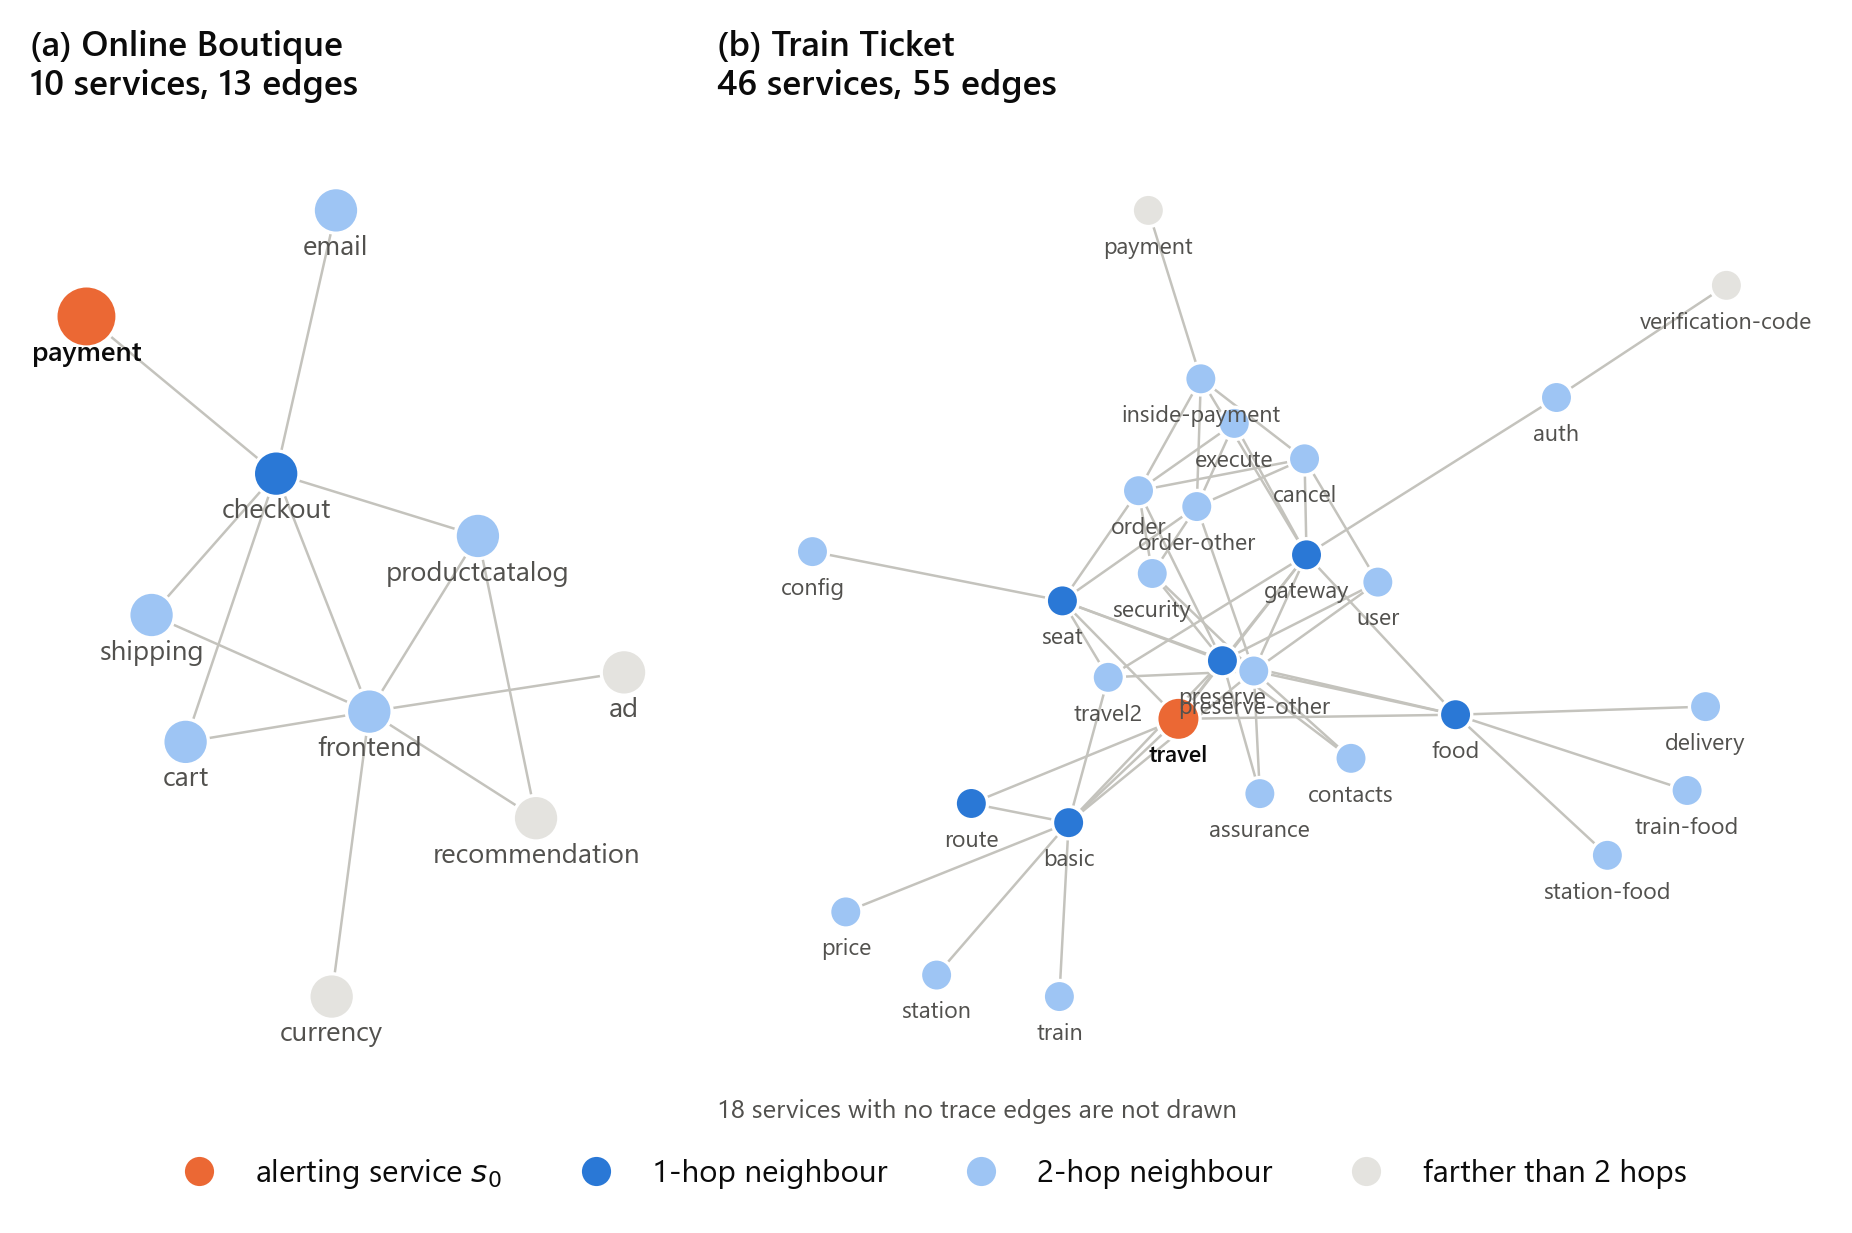
\includegraphics[width=\linewidth]{Images/C1/figures/ch2/h2.4-service-graph.png}
  \vspace{0.35cm}
  \caption[Đồ thị phụ thuộc service dựng từ trace của Nezha]{Đồ thị phụ thuộc service dựng từ trace của Nezha: (a)~OnlineBoutique (10 service, 13 cạnh) và (b)~TrainTicket (46 service, 55 cạnh), minh họa vùng mở rộng 1~hop và 2~hop quanh $s_0$.}
  \label{fig:ch2-service-graph}
\end{figure}

Ví dụ trên OnlineBoutique, khi \code{paymentservice} chậm, triệu chứng thường xuất hiện sớm ở các service gọi nó như \code{checkoutservice} (1~hop) và \code{frontend} (2~hop) trước khi thấy log lỗi tại chính \code{paymentservice}. Tuy nhiên, \textbf{gần trên đồ thị} không đồng nghĩa với \textbf{có quan hệ nhân quả}, và đồ thị chỉ phản ánh các đường gọi từng xuất hiện trong trace. Đề tài khai thác đồ thị cho hai nhiệm vụ: mở rộng ngữ cảnh truy xuất trong \CTAV{} (Mục~\ref{sec:ch4-c1}) và gom sự cố, lan truyền ngược trong tác tử \term{RCA}{RCA} (Mục~\ref{sec:ch4-rca}).

\subsubsection{Hợp nhất đa phương thức (\term{FusionScore}{Fusion Score}) và \term{RAG}{RAG} trong giám sát}
\label{sec:ch2-fusion}
\label{sec:ch2-rag}

\textbf{Retrieval-Augmented Generation} (\term{RAG}{RAG})~\cite{lewis2020rag} kết hợp bộ truy xuất với mô hình ngôn ngữ để đưa dữ liệu thời gian thực (log, span quanh cảnh báo) vào prompt thay vì để mô hình đoán từ tri thức tĩnh, giúp kết luận dẫn được về bằng chứng cụ thể. Tuy nhiên, truy xuất theo từ khóa đơn thuần (\term{BM25}{BM25}) dễ bỏ sót triệu chứng ở service lân cận không khớp từ khóa. \textbf{Truy xuất lai nhận biết topology} (\term{FusionScore}{Fusion Score}~\cite{icaetm2026}) giải quyết bằng cách gom ứng viên từ cả kênh \term{BM25}{BM25} lẫn các service trong bán kính $2$~hop, rồi xếp hạng theo tổ hợp tuyến tính của ba tín hiệu chuẩn hóa: mức khớp từ vựng ($\widehat{\text{BM25}}$), độ gần thời gian suy giảm theo hàm mũ quanh trung điểm cửa sổ $t_0$, và độ gần đồ thị $\text{GraphSim} = 1 / (1 + d_G)$.

Mặt trái của cơ chế hợp nhất này là khi cửa sổ thực chất bình thường, những sự kiện nền vô hại nhưng nằm rất sát $t_0$ hoặc gần trên đồ thị vẫn đạt điểm cao và lọt vào ngữ cảnh của LLM, dễ kích hoạt \term{ConfirmationBias}{thiên lệch xác nhận} (Mục~\ref{sec:ch2-thien-lech}). Công thức \term{FusionScore}{Fusion Score} đầy đủ, trọng số $(\alpha, \beta, \gamma)$ và cài đặt thành phần \comp{C1} được trình bày tại Mục~\ref{sec:ch4-c1}; ý tưởng liên quan dùng bằng chứng log/topology để cứu cửa sổ dưới ngưỡng metric được khảo sát qua cổng Rescue (\comp{C5}, chỉ là ablation) ở Mục~\ref{sec:ch4-detector}.

% -----------------------------------------------------------------------------
\subsection{LLM làm bộ thẩm định (LLM-as-a-Judge)}
\label{sec:ch2-judge}

Mục này giải thích cách một mô hình ngôn ngữ lớn được dùng để thẩm định cảnh báo, cách kiểm soát chi phí khi gọi nó, và các rủi ro về độ tin cậy mà phần đề xuất phải xử lý.

\subsubsection{LLM-as-a-Judge, đầu ra có cấu trúc và kiểm soát ngân sách}
\label{sec:ch2-prompt}
\label{sec:ch2-ngan-sach}

\textbf{LLM-as-a-Judge}~\cite{zheng2023judging} là cách dùng mô hình ngôn ngữ lớn để đánh giá hoặc phân loại đầu vào dựa trên tiêu chí cho trước. Trong vận hành hệ thống, LLM đọc trực tiếp log và thông điệp lỗi không cần huấn luyện lại, nhưng có ba hạn chế: độ trễ lớn, chi phí theo token và đầu ra không hoàn toàn tất định kể cả ở $\text{temperature} = 0$. Để tích hợp vào pipeline tự động, đầu ra phải bị ràng buộc theo \textbf{lược đồ JSON có cấu trúc} (nhãn phán quyết, mức ưu tiên, độ tin cậy, danh sách định danh bằng chứng hợp lệ, lý do và khuyến nghị) và được kiểm tra trước khi sử dụng.

Kết luận thô của judge chưa phải quyết định cuối mà đi qua một \textbf{chính sách quyết định}: chấp nhận cảnh báo, bác bỏ hoặc chuyển sang \code{manual\_review} khi thiếu bằng chứng hoặc dưới ngưỡng tin cậy — tương ứng nguyên lý phân loại có lựa chọn từ chối (\emph{reject option})~\cite{chow1970reject}. Để kiểm soát chi phí API dưới ràng buộc ngân sách $B$ lượt gọi theo thứ tự thời gian, cộng đồng thường dùng kiến trúc thẩm định theo tầng (\emph{cascade}, như FrugalGPT~\cite{chen2024frugalgpt}) kết hợp cơ chế bộ nhớ đệm (\emph{cache}) theo hàm băm của prompt để bảo đảm khả năng tái lập. Đặc tả lược đồ JSON, khóa cache \code{sha256}, mô hình cố định \code{gemini-2.5-flash} và các cơ chế định tuyến/chính sách của hệ thống được trình bày ở Mục~\ref{sec:ch4-policy}--\ref{sec:ch4-judge} và dùng trực tiếp cho chế độ demo ngoại tuyến ở Chương~\ref{ch:platform}.

\subsubsection{\term{ConfirmationBias}{Thiên lệch xác nhận}, hiệu chỉnh ngưỡng và nguồn gốc bằng chứng}
\label{sec:ch2-thien-lech}

\textbf{\term{ConfirmationBias}{Thiên lệch xác nhận}} (\emph{confirmation bias}) là xu hướng diễn giải bằng chứng theo hướng xác nhận giả định có sẵn; trên LLM, xu hướng đồng thuận với gợi ý trong prompt (\emph{sycophancy}) đã được ghi nhận rộng rãi~\cite{sharma2024sycophancy}. Khi prompt nêu rõ đang có cảnh báo và đính kèm bằng chứng sát thời điểm, judge dễ kết luận \code{true\_alert} ngay cả khi bằng chứng chỉ là hoạt động nền bình thường (minh họa ở Hình~\ref{fig:ch2-confirmation-bias}).

\begin{figure}[htbp]
  \centering
  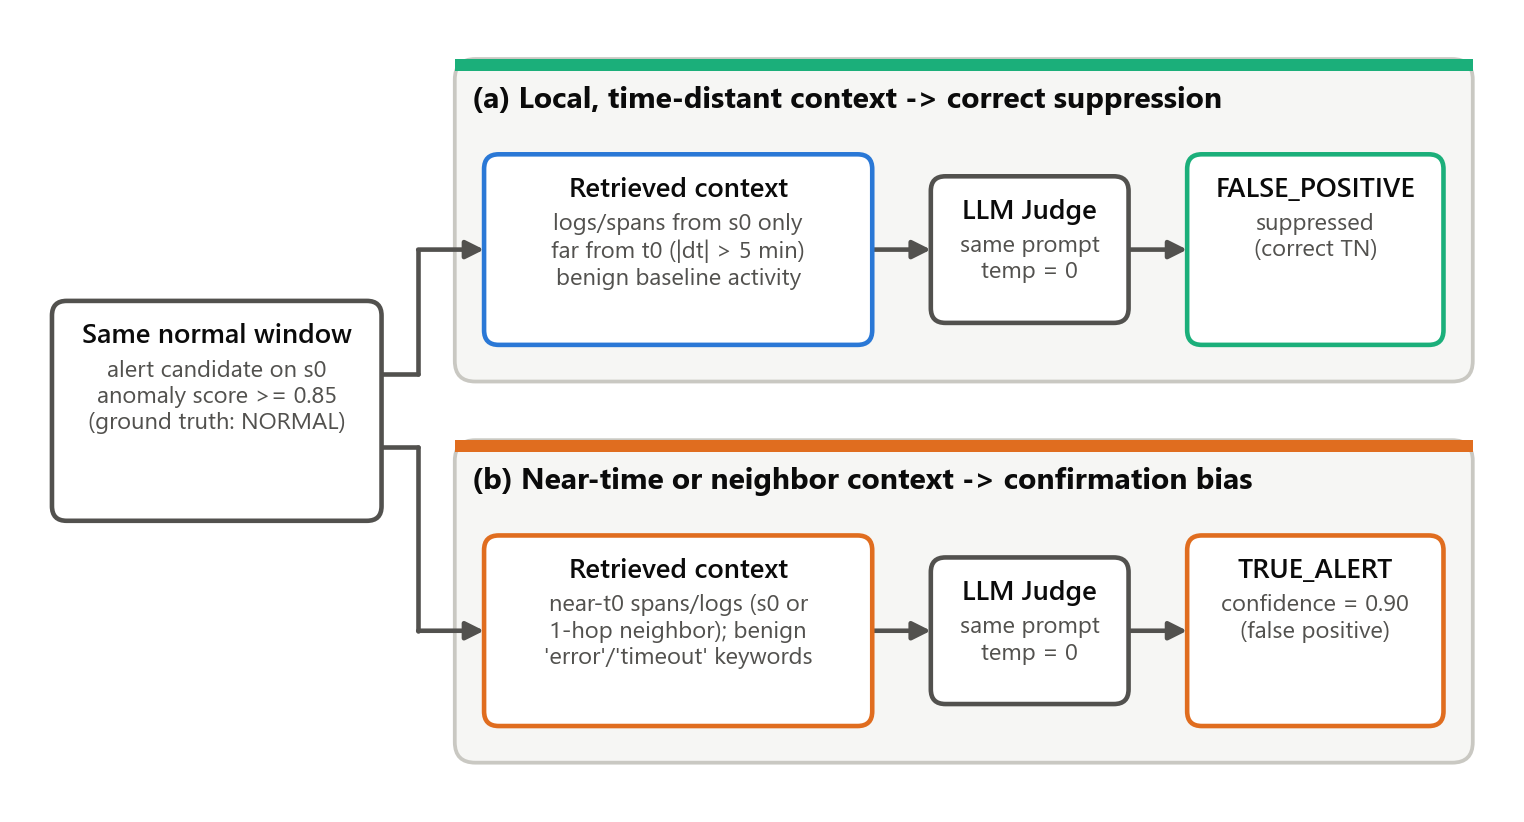
\includegraphics[width=\linewidth]{Images/C1/figures/ch2/h2.7-confirmation-bias.png}
  \vspace{0.35cm}
  \caption[Minh họa thiên lệch xác nhận của bộ thẩm định LLM]{\term{ConfirmationBias}{Thiên lệch xác nhận} của judge trên cùng một cửa sổ bình thường: (a)~ngữ cảnh xa thời điểm cảnh báo cho \code{false\_positive}; (b)~ngữ cảnh sát thời điểm hoặc từ lân cận dẫn tới \code{true\_alert} sai. \emph{(Nguồn: tác giả vẽ, có hỗ trợ AI.)}}
  \label{fig:ch2-confirmation-bias}
\end{figure}

\textbf{Hiệu chỉnh và nguồn gốc bằng chứng.} Một bộ phân loại được hiệu chỉnh tốt khi xác suất dự đoán khớp tần suất đúng thực tế~\cite{guo2017calibration}, nhưng độ tin cậy tự khai bằng lời của LLM thường co cụm ở vài mốc tròn và tự tin thái quá~\cite{xiong2024uncertainty}, buộc ngưỡng $\theta$ phải được chọn trên \splitname{val} thay vì hiểu theo nghĩa đen. Bên cạnh đó, \textbf{nguồn gốc bằng chứng} (\emph{provenance}) phân biệt bằng chứng thuộc chính service phát cảnh báo $s_0$ với bằng chứng từ láng giềng đồ thị. Đây là cơ sở lý thuyết của hai hướng thiết kế trong \CTAV{}: đặt ngưỡng bất đối xứng theo nguồn bằng chứng (\comp{C2}, đã loại sau kiểm định) và \textbf{neo bằng chứng bất thường tại $s_0$} theo phân vị nền đo từ \splitname{dev} (\comp{C3}, đang dùng — Mục~\ref{sec:ch4-policy}; bằng chứng cơ chế ở Mục~\ref{sec:ch5-h1}).

% -----------------------------------------------------------------------------
\subsection{Phân tích nguyên nhân gốc (\term{RCA}{RCA}) trên microservice}
\label{sec:ch2-rca}
\label{sec:ch2-gom}
\label{sec:ch2-lan-truyen}
\label{sec:ch2-bao-cao}

\textbf{Phân tích nguyên nhân gốc} (\emph{root cause analysis}, \term{RCA}{RCA}) nhằm xác định \textbf{service gốc} gây ra sự cố, tách biệt với các service chỉ chịu ảnh hưởng dây chuyền (\emph{cascade}). Khi một service lỗi, các service gọi nó (ngược chiều cạnh $u \to v$) thường chậm hoặc phát lỗi theo, tạo ra nhiều cảnh báo liên tiếp. Chuỗi xử lý \term{RCA}{RCA} tiêu chuẩn sau tầng thẩm định gồm ba bước: (1)~\textbf{gom cảnh báo thành sự cố (\emph{incident})} theo độ gần thời gian và tính liên thông trên đồ thị phụ thuộc; (2)~\textbf{lần ngược đồ thị gọi} để xếp hạng các service nghi vấn gốc (cần lưu ý giới hạn khi quan hệ gọi không đồng nghĩa nhân quả hoặc cảnh báo đầu vào bị thiếu); và (3)~\textbf{sinh báo cáo chẩn đoán có cấu trúc} (JSON) trích dẫn bằng chứng hợp lệ cho kỹ sư trực. Thuật toán gom nhóm, công thức bỏ phiếu lan truyền ngược 1 bước và bộ kiểm duyệt báo cáo cụ thể của tác tử \term{RCA}{RCA} được trình bày tại Mục~\ref{sec:ch4-rca}.

% -----------------------------------------------------------------------------
\subsection{Tiêu chí và phương pháp đánh giá}
\label{sec:ch2-danh-gia}

Mục này xác lập các thước đo hiệu năng và công cụ kiểm định thống kê dùng trong Chương~\ref{ch:thuc-nghiem}.

\subsubsection{Thước đo phân loại cảnh báo và định vị \term{RCA}{RCA}}
\label{sec:ch2-chi-so}
\label{sec:ch2-hitk}

Với bài toán thẩm định cảnh báo, mỗi cửa sổ được phân vào một trong bốn ô TP, FP, FN, TN và đánh giá bằng bốn chỉ số chuẩn: \textbf{Precision}, \textbf{Recall}, \textbf{F1} và \textbf{\term{FPR}{FPR}} ($\mathrm{FP}/(\mathrm{FP}+\mathrm{TN})$). Hai quy ước quan trọng được áp dụng xuyên suốt: (i)~Recall luôn tính trên \emph{toàn bộ} cửa sổ lỗi của split (kể cả cửa sổ bị detector bỏ sót) để tránh thổi phồng; và (ii)~vì dữ liệu mất cân bằng $1:135$, Precision và F1 rất nhạy với \term{FPR}{FPR} (như ví dụ Mục~\ref{sec:ch2-khoang-trong}), nên \term{FPR}{FPR} luôn được báo cáo tường minh bên cạnh số lần gọi LLM và chi phí token.

Với tác tử \term{RCA}{RCA}, mỗi sự cố có danh sách xếp hạng service; \textbf{\term{HitK}{Hit@k}} (dùng \term{HitK}{Hit@1} và \term{HitK}{Hit@3} ở mức service) đo tỷ lệ sự cố đơn lỗi mà service gốc nằm trong $k$ vị trí đầu (sự cố đa lỗi nhập nhằng bị loại khỏi \term{HitK}{Hit@k} và báo riêng). Mức nén cảnh báo được đo bằng \textbf{Alert Reduction Ratio} (\term{ARR}{ARR}):
\begin{equation}
  \mathrm{ARR} = 1 - \frac{\text{số incident}}{\text{số cảnh báo}}.
  \label{eq:ch2-arr}
\end{equation}
Baseline định vị là xếp hạng theo điểm bất thường cực đại trong sự cố; ngoài ra tỷ lệ báo cáo JSON hợp lệ cũng được theo dõi (Mục~\ref{sec:ch5-rca}).

\subsubsection{Bootstrap CI và kiểm định McNemar}
\label{sec:ch2-thong-ke}

Do số cửa sổ lỗi mỗi split chỉ ở mức vài trăm, đề tài dùng hai công cụ phi tham số (mức ý nghĩa $\alpha = 0{,}05$, hai phía) để tách tín hiệu khỏi nhiễu:
\begin{itemize}[label=--]
  \item \textbf{Bootstrap ghép cặp (CI95)}~\cite{efron1993bootstrap}: lấy mẫu lại có hoàn lại $N$ cửa sổ $1.000$ lần (\code{seed = 42}) đồng thời cho hai phương pháp $A$ và $B$ để tính khoảng tin cậy 95\% phân vị của hiệu $\Delta = \text{chỉ số}(A) - \text{chỉ số}(B)$; nếu CI95 chứa $0$ thì chưa đủ bằng chứng kết luận khác biệt.
  \item \textbf{Kiểm định McNemar chính xác}~\cite{mcnemar1947note}: so sánh hai bộ phân loại trên cùng tập cửa sổ dựa trên số ca bất đồng ($b$: $A$ đúng, $B$ sai; $c$: $A$ sai, $B$ đúng), với giá trị $p$ hai phía:
  \begin{equation}
    n = b + c, \qquad
    p = \min\!\left(1,\; 2 \sum_{i=0}^{\min(b, c)} \binom{n}{i} 0{,}5^n\right).
    \label{eq:ch2-mcnemar}
  \end{equation}
\end{itemize}
\hyp{H2} là giả thuyết chính; với các giả thuyết phụ, $p$ được báo thô không hiệu chỉnh đa so sánh (Mục~\ref{sec:ch7-hop-le}). Độ dao động lặp lại của judge được đo riêng bằng \code{repeat} $\in \{0, 1, 2\}$ trên mẫu 200 cửa sổ (Mục~\ref{sec:ch5-repeat}).

% -----------------------------------------------------------------------------
\subsection{Giả thuyết nghiên cứu và đăng ký trước}
\label{sec:ch2-dang-ky}

\textbf{Đăng ký trước} (\emph{pre-registration}) ghi cố định giả thuyết, phép so sánh và tiêu chí bác bỏ \emph{trước} khi chạy trên tập kiểm định để ngăn tinh chỉnh hậu nghiệm. Đề tài tuân thủ ba quy tắc: mọi chọn lọc tham số chỉ thực hiện trên \splitname{dev} và \splitname{val}; tập \splitname{test} chỉ chạy đúng một lần sau khi khóa bản đăng ký \hyp{H0}--\hyp{H5} (ngày 14/11/2026, với \hyp{H2} là giả thuyết chính có biên $\delta = 0{,}05$, \hyp{H1} chỉ chạy trên mẫu cố định của \splitname{val}); mọi sai lệch phát sinh đều được ghi nhận minh bạch thay vì sửa ngược. Bảng đầy đủ tiêu chí \hyp{H0}--\hyp{H5} đặt tại Bảng~\ref{tab:h0-h5} (Mục~\ref{sec:ch5-hypotheses}).

% -----------------------------------------------------------------------------
\subsection{Công nghệ nền tảng}
\label{sec:ch2-cong-nghe}

Bảng~\ref{tab:ch2-cong-nghe} tóm tắt các công nghệ hiện thực hệ thống cùng vai trò và lý do lựa chọn (cách lắp ráp thành hệ thống hoàn chỉnh trình bày tại Mục~\ref{sec:ch4-impl}). Đề tài cố định một mô hình API duy nhất (\code{gemini-2.5-flash}, $\text{temperature} = 0$, qua cache) cho mọi phương pháp để loại trừ nhiễu đổi mô hình, đồng thời tách vai trò lưu trữ giữa ClickHouse (dữ liệu sự kiện cột phục vụ truy vấn tổng hợp) và PostgreSQL (dữ liệu quan hệ cho sự cố và báo cáo chẩn đoán).

\begin{table}[H]
  \centering
  \caption{Công nghệ nền tảng: vai trò trong hệ và lý do chọn.}
  \label{tab:ch2-cong-nghe}
  \tblfont
  \tblsetup
  \begin{tabularx}{\linewidth}{|>{\raggedright\arraybackslash}p{3.4cm}|>{\raggedright\arraybackslash}p{1.9cm}|Y|Y|}
    \hline
    \rowcolor{gray!15}
    \textbf{Công nghệ} & \textbf{Phiên bản} & \textbf{Vai trò trong hệ} & \textbf{Lý do chọn} \\
    \hline
    Python~\cite{python2026docs} & $\ge 3.11$ & Ngôn ngữ của mọi service, harness thực nghiệm và script & Hệ sinh thái khoa học dữ liệu; một ngôn ngữ cho cả thực nghiệm lẫn hệ thống \\
    \hline
    scikit-learn~\cite{pedregosa2011sklearn} & $\ge 1.4$ & Isolation Forest của bộ phát hiện & Cài đặt chuẩn, có kiểm thử, tham số rõ ràng \\
    \hline
    Gemini API~\cite{google2026gemini} (\code{gemini-2.5-flash}) & REST \code{v1beta} & Judge của \CTAV{} và bộ tóm tắt của tác tử \term{RCA}{RCA} & Một model API cố định cho mọi phương pháp; trả JSON; chi phí thấp cho hàng chục nghìn lần gọi \\
    \hline
    ClickHouse~\cite{clickhouse2026docs} & 24.3 & Lưu mọi kết luận của judge cùng bằng chứng, phục vụ truy vấn phân tích & Cơ sở dữ liệu cột, truy vấn tổng hợp nhanh trên hàng chục nghìn candidate \\
    \hline
    PostgreSQL~\cite{postgresql2026docs} & 16 & Lưu incident và báo cáo chẩn đoán & Dữ liệu quan hệ, có ràng buộc, cần tính toàn vẹn \\
    \hline
    FastAPI~\cite{fastapi2026docs} & $\ge 0.110$ & API chỉ đọc cho dashboard & Kiểu dữ liệu tường minh qua Pydantic, tài liệu API tự sinh \\
    \hline
    React~\cite{react2026docs} và Vite~\cite{vite2026docs} & React 19, Vite 8 & Dashboard năm màn hình & Giao diện thành phần; tách gói theo màn hình, hỗ trợ chạy tĩnh ngoại tuyến \\
    \hline
    Docker Compose~\cite{docker2026compose} & --- & Triển khai toàn hệ bằng một lệnh, hai profile \code{dev} và \code{full} & Tái lập môi trường trên máy khác, kể cả lúc demo \\
    \hline
  \end{tabularx}
\end{table}

% -----------------------------------------------------------------------------
\subsection{Kết chương}
\label{sec:ch2-ket-chuong}

Chương này đã xác lập hệ thống kiến thức và công nghệ nền tảng theo đúng luồng xử lý của đề tài: đơn vị cửa sổ $60\,\text{s}$ và bộ dữ liệu Nezha; bộ phát hiện Isolation Forest cùng khoảng trống ngữ nghĩa; truy xuất bằng chứng \term{BM25}{BM25}, đồ thị phụ thuộc service và nguyên lý \term{RAG}{RAG} lai; cơ chế \emph{LLM-as-a-Judge}, \term{ConfirmationBias}{thiên lệch xác nhận} và hiệu chỉnh theo nguồn gốc bằng chứng; bài toán \term{RCA}{RCA} trên microservice; cùng khung đánh giá thống kê (bootstrap CI, McNemar, đăng ký trước) và ngăn xếp công nghệ hiện thực. Mọi thành phần đề xuất ở Chương~\ref{ch:de-xuat}, mọi phép kiểm định ở Chương~\ref{ch:thuc-nghiem} và toàn bộ platform trình diễn ở Chương~\ref{ch:platform} đều dựa trực tiếp trên các khái niệm này, cho thấy nền tảng lý thuyết và kỹ thuật đã đầy đủ để chuyển sang khảo sát công trình liên quan và thiết kế hệ thống.

 \newpage
 % =============================================================================
% Chuong 3: Cong trinh lien quan
% =============================================================================
% Cach dung tren Overleaf:
%   1. Bao dam da tai macros.tex, refs.bib va chapters/ch3.tex vao du an.
%   2. Trong main.tex:
%        \input{macros}
%        ...
%        \include{chapters/ch3}
%        ...
%        \bibliographystyle{IEEEtran}
%        \bibliography{refs}
%
% Cac nhan lien chuong duoc tham chieu tu Chuong 3:
%   Chuong: ch:mo-dau, ch:nen-tang, ch:de-xuat, ch:thuc-nghiem, ch:platform
%   Chuong 2: sec:ch2-du-lieu, sec:ch2-truy-xuat, sec:ch2-judge, sec:ch2-rca,
%             sec:ch2-dang-ky
%   Chuong 4: sec:ch4-ctav, sec:ch4-c1, sec:ch4-policy, sec:ch4-c4, sec:ch4-rca
%   Chuong 5: sec:ch5-hypotheses, sec:ch5-c5, sec:ch5-budget
% =============================================================================

\section{Công trình liên quan}
\label{ch:cong-trinh-lien-quan}

Chương này hệ thống hóa các hướng nghiên cứu và các hệ thống vận hành thực tế liên quan trực tiếp tới bài toán thẩm định cảnh báo có nhận biết topology và phân tích nguyên nhân gốc trên kiến trúc microservice. Nội dung được tổ chức xoay quanh hai câu hỏi: cộng đồng học thuật và công nghiệp đã giải quyết những khía cạnh nào của chuỗi xử lý từ phát hiện bất thường đến định vị nguyên nhân gốc, và còn những khoảng trống nào mà đề xuất của đề tài nhắm tới. Mục~\ref{sec:ch3-nghien-cuu} khảo sát bảy nhánh nghiên cứu học thuật từ phát hiện bất thường chuỗi thời gian, ứng dụng mô hình ngôn ngữ lớn trong phân tích log và nguyên nhân gốc, kiến trúc giám sát lai, phân tích nguyên nhân gốc dựa trên đồ thị, truy xuất dựa trên đồ thị, hiệu chỉnh độ tin cậy của \emph{LLM-as-a-Judge}, đến gom nhóm và phân loại cảnh báo. Mục~\ref{sec:ch3-he-thong} đối chiếu các nền tảng AIOps thương mại và công cụ mã nguồn mở hiện hành dựa trên tài liệu chính thức. Cuối cùng, Mục~\ref{sec:ch3-ket-chuong} tổng hợp các hướng tiếp cận trong Bảng~\ref{tab:ch3-so-sanh-nc} và Bảng~\ref{tab:ch3-so-sanh-ht}, rút ra bốn khoảng trống nghiên cứu và định vị rõ phạm vi đóng góp của \CTAV{} cùng tác tử phân tích nguyên nhân gốc.

% -----------------------------------------------------------------------------
\subsection{Các nghiên cứu liên quan}
\label{sec:ch3-nghien-cuu}

Các công trình liên quan đến đề tài nằm ở giao điểm giữa giám sát chuỗi thời gian, phân tích dữ liệu quan sát đa phương thức, truy xuất bằng chứng theo đồ thị và hiệu chỉnh mô hình ngôn ngữ lớn đóng vai trò bộ thẩm định. Bảy tiểu mục dưới đây phân tích từng nhánh theo cùng một trục: cách tiếp cận của công trình, hạn chế đặt trong bài toán của đề tài và điểm khác biệt của đề tài.

\subsubsection{Phát hiện bất thường trên chuỗi thời gian metric}
\label{sec:ch3-tsad}

Các phương pháp phát hiện bất thường chuỗi thời gian không giám sát chia thành hai nhóm chính. Nhóm cây phân tách ngẫu nhiên gồm Isolation Forest~\cite{isof} (cô lập điểm bất thường theo độ sâu cây, nhẹ và không cần nhãn) và Robust Random Cut Forest (RRCF)~\cite{guha2016robust} (cập nhật cây trực tuyến trên luồng dữ liệu biến đổi). Nhóm học sâu đồ thị như MTAD-GAT~\cite{zhao2020multivariate} (chú ý đồ thị song song theo đặc trưng và thời gian) và GDN~\cite{deng2021graph} (tự học đồ thị cảm biến để dự báo độ lệch) khai thác tốt tương quan đa biến, nhưng đòi hỏi huấn luyện lại khi topology thay đổi và tốn tài nguyên tính toán. Hạn chế chung của cả hai nhóm là chỉ dựa vào tín hiệu số mà bỏ qua ngữ cảnh văn bản từ log hay vết thực thi trace, nên dễ báo động giả trước dao động tải bình thường. Đề tài vì vậy giữ tầng lọc nhẹ bằng Isolation Forest để bảo đảm tốc độ và khả năng tái lập, rồi chuyển trọng tâm sang tầng thẩm định bằng bằng chứng đa phương thức phía sau.

\subsubsection{Mô hình ngôn ngữ lớn trong phân tích log và nguyên nhân gốc}
\label{sec:ch3-llm-log-rca}

Ở tầng xử lý log phi cấu trúc, LogParser-LLM~\cite{zhong2024logparser} kết hợp cây tiền tố với truy vấn LLM chọn lọc để tách mẫu log linh hoạt, còn LogLLM~\cite{wang2024logllm} phối hợp bộ mã hóa ngữ nghĩa dạng BERT với bộ giải mã LLM để phát hiện bất thường trên chuỗi log; tuy nhiên cả hai chỉ làm việc trên log đơn lẻ mà chưa nối với luồng cảnh báo metric hay đồ thị phụ thuộc dịch vụ.

Ở tầng phân tích nguyên nhân gốc cho sự cố đám mây, Ahmed và cộng sự~\cite{ahmed2023recommending} dùng dòng mô hình GPT để khuyến nghị nguyên nhân gốc và hướng khắc phục trên hơn 40.000 sự cố Microsoft, RCACopilot~\cite{chen2024rcacopilot} tự động hóa thu thập dữ liệu chẩn đoán theo loại sự cố, trong khi RCAgent~\cite{rcagent2023} và khảo sát tác tử ReAct của Roy và cộng sự~\cite{roy2024exploring} trang bị công cụ truy vấn log--metric để LLM tự điều tra sự cố. Hạn chế chung là phần lớn các công trình này giả định sự cố đầu vào đã được xác nhận sẵn và đánh giá trên dữ liệu nội bộ khó tái lập, bỏ qua khâu thẩm định luồng cảnh báo thô để chặn báo động giả trước khi gọi tác tử tốn kém. Đề tài đặt tầng thẩm định \CTAV{} có kiểm soát ngân sách ngay trước tác tử \term{RCA}{RCA} trên bộ dữ liệu công khai tái lập được.

\subsubsection{Kiến trúc giám sát lai và LLM-as-a-Judge}
\label{sec:ch3-hybrid-judge}

Để dung hòa chi phí gọi LLM với yêu cầu giám sát liên tục, nhiều công trình kết hợp mô hình nhẹ hoặc cơ chế truy xuất tăng cường sinh (\emph{Retrieval-Augmented Generation}, \term{RAG}{RAG})~\cite{lewis2020rag} với bộ phân xử LLM ở tầng sau. Về nguyên lý phân tầng chi phí, nền tảng lý thuyết bắt nguồn từ cơ chế đánh đổi sai số và quyền từ chối (\emph{reject option}) của Chow~\cite{chow1970reject} cùng mô hình chuỗi tầng gọi LLM tiết kiệm chi phí FrugalGPT của Chen và cộng sự~\cite{chen2024frugalgpt}, trong đó các mẫu rõ ràng được xử lý bởi mô hình rẻ hơn và chỉ vùng bất định mới chuyển lên mô hình đắt hơn.

Trong miền phát hiện bất thường, một loạt công trình gần đây đưa kiến trúc lai vào thực nghiệm. Russell-Gilbert và cộng sự~\cite{raad-llm} đề xuất RAAD-LLM, tích hợp \term{RAG}{RAG} vào LLM để thích nghi phát hiện bất thường chuỗi thời gian khi bối cảnh hệ thống thay đổi mà không cần tinh chỉnh trọng số. Gu và cộng sự~\cite{argos} giới thiệu ARGOS, một khuôn khổ tác tử cho phép LLM tự sinh và tinh chỉnh luật phát hiện bất thường trên chuỗi thời gian nhằm giảm phụ thuộc vào truy vấn trực tiếp trên từng mẫu. Devireddy và Huang~\cite{calm} đề xuất CALM, điều phối liên tục giữa phát hiện thời gian thực và cơ chế can thiệp thích nghi của LLM. Ở góc độ đánh giá năng lực thẩm định, Sivalingam và cộng sự~\cite{judge} xây dựng TSQueryBench để kiểm tra khả năng dùng \emph{LLM-as-a-Judge} đánh giá lời giải thích bất thường chuỗi thời gian.

Hạn chế chung của các kiến trúc lai này khi áp vào microservice là chúng chủ yếu vận hành trên chuỗi thời gian đơn lẻ hoặc truy xuất ngữ cảnh văn bản phẳng, chưa kết nối tường minh với đồ thị phụ thuộc giữa các service sinh từ trace. Quan trọng hơn, các nghiên cứu này chưa khảo sát hệ quả ngược chiều khi mở rộng bằng chứng cho bộ thẩm định LLM: việc mở rộng ngữ cảnh theo topology có thể làm tăng tỷ lệ báo động giả theo kiểu \term{ConfirmationBias}{thiên lệch xác nhận}, và chưa rõ yếu tố nào trong ngữ cảnh gây ra hiện tượng này. Đề tài này tập trung giải quyết trực tiếp bài toán kiểm soát ngân sách và kìm báo động giả trong kiến trúc lai detector nhẹ kết hợp \emph{LLM-as-a-Judge} cho hệ microservice.

\subsubsection{Phân tích nguyên nhân gốc dựa trên topology, đồ thị và suy luận nhân quả}
\label{sec:ch3-rca-graph}

Định vị nguyên nhân gốc dựa trên đồ thị phụ thuộc và suy luận nhân quả là nhánh phát triển lâu đời nhất trong giám sát hệ phân tán. Kim và cộng sự~\cite{kim2013monitorrank} đề xuất MonitorRank, thực hiện bước đi ngẫu nhiên (\emph{random walk}) có trọng số tương quan metric trên đồ thị gọi dịch vụ để xếp hạng service nghi vấn trong kiến trúc hướng dịch vụ. Chen và cộng sự~\cite{chen2014causeinfer} xây dựng CauseInfer với đồ thị nhân quả hai tầng (tầng dịch vụ và tầng metric) bằng thuật toán kiểm định độc lập có điều kiện PC để lần ngược nút gốc gây suy giảm hiệu năng. Trên kiến trúc microservice, Wu và cộng sự~\cite{wu2020microrca} giới thiệu MicroRCA, gắn dữ liệu sử dụng tài nguyên máy chủ vào đồ thị dịch vụ bất thường và áp dụng Personalized PageRank để định vị service gây lỗi hiệu năng.

Các công trình gần đây tiếp cận bài toán bằng mô hình nhân quả chặt chẽ hơn và dữ liệu đa phương thức. Li và cộng sự~\cite{li2022circa} đề xuất CIRCA, mô hình hóa lỗi như một can thiệp (\emph{intervention}) trên mạng Bayes nhân quả xây từ kiến trúc hệ thống và dùng điều kiện thay đổi phân bố có điều kiện để chỉ ra chỉ số gốc. Ikram và cộng sự~\cite{ikram2022rcd} đề xuất RCD, xem sự cố như can thiệp cục bộ và khám phá đồ thị nhân quả theo phân cấp để tránh chi phí tính toán lớn của thuật toán PC trên toàn bộ hệ thống. Kết hợp cả ba trụ cột dữ liệu quan sát, Yu và cộng sự~\cite{nezha} đề xuất Nezha, chuyển đổi metric, log và trace thành biểu diễn sự kiện đồng nhất và so sánh mẫu phân kỳ giữa trạng thái bình thường với trạng thái lỗi để định vị nguyên nhân gốc ở mức chi tiết, đồng thời công bố bộ dữ liệu microservice đa phương thức làm chuẩn đánh giá. Đáng lưu ý về tính bền vững của chuỗi xử lý, Pham và cộng sự~\cite{pham2024baro} đề xuất BARO bằng phát hiện điểm đổi Bayes đa biến kết hợp kiểm định phi tham số, đồng thời chỉ ra rằng sai số ở khâu phát hiện bất thường đầu vào có thể lan sang làm giảm mạnh độ chính xác định vị gốc; tiếp đó nhóm tác giả công bố bộ chuẩn RCAEval~\cite{pham2025rcaeval} tổng hợp 735 ca lỗi đa phương thức trên nhiều hệ microservice mã nguồn mở để thống nhất việc so sánh.

Hạn chế của nhóm phương pháp đồ thị và nhân quả thuần túy gồm hai điểm. Thứ nhất, phần lớn mô hình chỉ xuất ra danh sách xếp hạng service hoặc metric gốc dưới dạng chỉ số toán học, thiếu báo cáo tường minh giải thích cơ chế lan truyền bằng chứng từ log và trace cho kỹ sư vận hành. Thứ hai, trừ những phân tích gần đây như BARO, đa số nghiên cứu \term{RCA}{RCA} giả định cửa sổ thời gian sự cố đã được xác định sạch từ trước, tách rời khỏi bài toán lọc cảnh báo giả trực tuyến. Đề tài này nối trực tiếp hai khâu: dùng \CTAV{} để làm sạch luồng cảnh báo trước khi gom sự cố, rồi dùng tác tử \term{RCA}{RCA} lần ngược chuỗi lan truyền trên đồ thị phụ thuộc và sinh báo cáo có cấu trúc kèm trích dẫn bằng chứng.

\subsubsection{Truy xuất dựa trên đồ thị và GraphRAG cho vận hành hệ thống}
\label{sec:ch3-graphrag}

Trong lĩnh vực xử lý ngôn ngữ tự nhiên, Edge và cộng sự~\cite{edge2024graphrag} đề xuất GraphRAG nhằm khắc phục hạn chế của truy xuất văn bản phẳng khi cần tổng hợp thông tin phân tán trên nhiều tài liệu. Phương pháp xây dựng đồ thị tri thức thực thể--quan hệ từ kho văn bản, phân cụm cộng đồng đồ thị và sinh tóm tắt phân cấp để trả lời các truy vấn mang tính toàn cục. Tuy mở ra hướng truy xuất có cấu trúc, GraphRAG thiết kế cho kho tài liệu tĩnh với đồ thị trích xuất bằng LLM, nên vừa tốn chi phí lập chỉ mục vừa khác về bản chất so với đồ thị phụ thuộc động của hệ microservice được đo trực tiếp từ quan hệ gọi \code{SpanID}--\code{ParentID} trong trace.

Khi áp dụng tư tưởng truy xuất theo cấu trúc đồ thị vào bài toán thẩm định cảnh báo microservice, một nghiên cứu tiền đề về truy xuất bằng chứng có nhận biết topology~\cite{icaetm2026} đã đề xuất kết hợp điểm từ khóa \term{BM25}{BM25} với độ gần về thời gian và khoảng cách bước nhảy trên đồ thị phụ thuộc service để cung cấp thêm bằng chứng từ các service láng giềng cho bộ thẩm định LLM (chi tiết công thức hợp nhất đã trình bày ở Mục~\ref{sec:ch2-truy-xuat}). Kết quả định tính của hướng tiếp cận này cho thấy một đánh đổi rõ rệt: việc mở rộng ngữ cảnh sang các service có liên kết gọi giúp cải thiện khả năng nhận diện các sự cố lan truyền mà bằng chứng cục bộ không đủ, nhưng khi đưa trực tiếp vào \emph{LLM-as-a-Judge} mà không có cơ chế kiểm soát chính sách, số báo động giả trên cửa sổ bình thường tăng mạnh. Nghiên cứu đó cho rằng hiện tượng này phù hợp với thiên lệch xác nhận do ngữ cảnh, nhưng chưa cô lập được yếu tố nào trong ngữ cảnh gây ra nó. Đề tài này xuất phát trực tiếp từ đánh đổi đó: trước hết cô lập yếu tố trong ngữ cảnh khiến judge xác nhận nhầm, sau đó xây dựng chính sách hiệu chỉnh quyết định trên bằng chứng và kiểm định nghiêm ngặt hiệu quả kìm báo động giả trên dữ liệu ngoài tập tinh chỉnh.

\subsubsection{Hiệu chỉnh độ tin cậy, thiên lệch của LLM-as-a-Judge và gắn bằng chứng}
\label{sec:ch3-calibration}

Dù \emph{LLM-as-a-Judge} đạt mức đồng thuận cao với người đánh giá trên nhiều tác vụ tổng quát~\cite{zheng2023judging}, hàng loạt nghiên cứu đã chứng minh mô hình ngôn ngữ mắc nhiều thiên lệch có hệ thống và thường tự tin thái quá. Wang và cộng sự~\cite{wang2024fair} chỉ ra rằng bộ thẩm định LLM chịu thiên lệch vị trí nghiêm trọng khi so sánh cặp câu trả lời, dẫn đến thứ hạng dễ bị thao túng chỉ bằng cách đảo thứ tự trình bày, và đề xuất khung FairEval hiệu chỉnh bằng cách buộc sinh bằng chứng trước khi chấm điểm kết hợp trung bình hóa vị trí. Sharma và cộng sự~\cite{sharma2024sycophancy} phân tích hiện tượng chiều lòng (\emph{sycophancy}), cho thấy mô hình đã qua tinh chỉnh theo phản hồi con người có xu hướng đồng thuận với giả định ngầm trong câu hỏi ngay cả khi giả định đó sai — một cơ chế tương đồng trực tiếp với \term{ConfirmationBias}{thiên lệch xác nhận} khi bộ thẩm định nhận thông báo rằng ``cảnh báo đang kích hoạt''.

Về hiệu chỉnh xác suất và ước lượng độ bất định, Guo và cộng sự~\cite{guo2017calibration} chứng minh các mạng nơ-ron hiện đại tuy chính xác nhưng hiệu chỉnh kém và đề xuất phương pháp hiệu chỉnh hậu xử lý bằng tỉ lệ nhiệt độ (\emph{temperature scaling}). Trên LLM, Kadavath và cộng sự~\cite{kadavath2022mostly} khảo sát khả năng mô hình tự đánh giá xác suất đúng của phát biểu do chính nó sinh ra, cho thấy tín hiệu nội tại có thể hiệu chỉnh được trong câu hỏi trắc nghiệm nhưng khó khái quát khi chuyển phân bố tác vụ. Gần hơn với bài toán sử dụng API thương mại không truy cập được xác suất token thô, Xiong và cộng sự~\cite{xiong2024uncertainty} đánh giá thực nghiệm độ tin cậy bằng lời (\emph{verbalized confidence}) trên nhiều dòng LLM và chỉ ra mô hình thường gán điểm tin cậy quá cao, tập trung dày đặc ở vùng sát $1{,}0$. Song song đó, để hạn chế suy diễn vô căn cứ trong văn bản sinh ra, Gao và cộng sự~\cite{gao2023alce} đề xuất chuẩn đánh giá ALCE đo đồng thời tính đúng đắn và chất lượng trích dẫn nguồn bằng chứng trong câu trả lời của LLM.

Khoảng trống còn lại trong nhánh nghiên cứu này là các kỹ thuật hiệu chỉnh hiện có chủ yếu thiết kế cho bài toán chấm điểm cặp câu trả lời, hỏi--đáp mở hoặc sinh văn bản có trích dẫn tổng quát. Chưa có cơ chế nào hiệu chỉnh trực tiếp quyết định của \emph{LLM-as-a-Judge} trong bài toán thẩm định cảnh báo microservice theo \emph{nguồn gốc bằng chứng} (nội bộ hay láng giềng trên đồ thị phụ thuộc) và theo \emph{mức độ bất thường nền đo trên tập phát triển}. Đề tài này cụ thể hóa ý tưởng hiệu chỉnh bằng chính sách neo bằng chứng và kiểm định tách biệt từng thành phần thiết kế (ngưỡng bất đối xứng theo nguồn bằng chứng, neo ngưỡng nền trên tập phát triển và định tuyến hai tầng) theo quy trình đăng ký giả thuyết trước ở Mục~\ref{sec:ch2-dang-ky}.

\subsubsection{Gom nhóm, phân loại và cứu cảnh báo trong vận hành}
\label{sec:ch3-alert-triage}

Để giảm tải bão cảnh báo trong vận hành trực tuyến, Zhao và cộng sự~\cite{zhao2020alertstorm} phát hiện thời điểm bão và gom cảnh báo tương quan thời gian--ngữ nghĩa thành cụm sự cố; Chen và cộng sự~\cite{chen2019empirical,chen2019continuous} phân tích lỗi định tuyến sự cố và xây dựng cơ chế phân loại liên tục; còn Kuang và cộng sự~\cite{kuang2024knowledge} kết hợp đặc trưng văn bản với tri thức vận hành và topology để gom cảnh báo cùng gốc. Các công trình này chủ yếu nén cảnh báo \emph{sau khi phát sinh} mà không thẩm định lại bản thân cảnh báo metric có phải báo động giả hay không, cũng ít kiểm chứng xem liệu có thể ``cứu'' các cửa sổ dưới ngưỡng metric bằng log/topology mà không làm tăng \term{FPR}{FPR} hay không. Đề tài tách rõ hai vai trò: dùng gom nhóm thời gian--topology ở đầu vào tác tử \term{RCA}{RCA} trên các cảnh báo đã được \CTAV{} xác nhận, và kiểm chứng cơ chế cứu cảnh báo (\code{Rescue Score}, \comp{C5}) như một phân tích loại trừ độc lập (Mục~\ref{sec:ch5-c5}).

% -----------------------------------------------------------------------------
\subsection{Các hệ thống và công cụ hiện có}
\label{sec:ch3-he-thong}
\label{sec:ch3-thuong-mai}
\label{sec:ch3-ma-nguon-mo}

Bên cạnh các nghiên cứu học thuật, Bảng~\ref{tab:ch3-he-thong-tm} và Bảng~\ref{tab:ch3-he-thong-mnm} lần lượt đối chiếu ba nền tảng AIOps thương mại và ba công cụ mã nguồn mở tiêu biểu dựa trên tài liệu chính thức của nhà phát triển.

\begin{table}[H]
  \centering
  \caption[Đối chiếu các nền tảng AIOps thương mại tiêu biểu]{Cơ chế cốt lõi và giới hạn của ba nền tảng AIOps thương mại tiêu biểu.}
  \label{tab:ch3-he-thong-tm}
  \tblfont
  \tblsetup
  \setlength{\tabcolsep}{4pt}
  \begin{tabularx}{\linewidth}{|>{\raggedright\arraybackslash}p{2.9cm}|Y|Y|}
    \hline
    \rowcolor{gray!15}
    \textbf{Nền tảng thương mại} & \textbf{Cơ chế cốt lõi (theo tài liệu chính thức)} & \textbf{Giới hạn đối với bài toán đề tài} \\
    \hline
    Datadog (Event Mgmt \& Bits AI)~\cite{datadog2026docs} & Gom cảnh báo theo topology, nhãn và thời gian; tác tử Bits AI kiểm định song song nhiều giả thuyết trên metric, log, trace. & Kiến trúc đóng kín; không công bố hiệu chỉnh LLM theo nguồn bằng chứng hay đánh giá độc lập tác động topology lên FP. \\
    \hline
    Dynatrace (Davis AI \& Smartscape)~\cite{dynatrace2026docs} & Bản đồ phụ thuộc Smartscape thời gian thực từ OneAgent; Davis AI phân tích cây lỗi tất định tách nút gốc và nút ảnh hưởng. & Gắn chặt hạ tầng thu thập độc quyền, chi phí cao; không giải bài toán hiệu chỉnh \emph{LLM-as-a-Judge} dưới ngân sách giới hạn. \\
    \hline
    PagerDuty AIOps~\cite{pagerduty2026docs} & Gom cảnh báo bằng học máy (\emph{Intelligent Alert Grouping}), gợi ý nguồn gốc theo lịch sử 6 tháng (\emph{Probable Origin}) và luật \emph{Event Orchestration}. & Phụ thuộc lịch sử sự cố tổ chức; không khai thác đồ thị trace từng cửa sổ để thẩm định tín hiệu thô hay kìm FP của LLM. \\
    \hline
  \end{tabularx}
\end{table}

\begin{table}[H]
  \centering
  \caption[Đối chiếu các công cụ quản lý cảnh báo và điều tra mã nguồn mở]{Cơ chế cốt lõi và giới hạn của ba công cụ mã nguồn mở tiêu biểu.}
  \label{tab:ch3-he-thong-mnm}
  \tblfont
  \tblsetup
  \setlength{\tabcolsep}{4pt}
  \begin{tabularx}{\linewidth}{|>{\raggedright\arraybackslash}p{2.9cm}|Y|Y|}
    \hline
    \rowcolor{gray!15}
    \textbf{Công cụ mã nguồn mở} & \textbf{Cơ chế cốt lõi (theo tài liệu chính thức)} & \textbf{Giới hạn đối với bài toán đề tài} \\
    \hline
    Prometheus Alertmanager~\cite{prometheus2026alertmanager} & Định tuyến (\code{route}), gom nhóm (\code{group\_by}), ức chế (\code{inhibit\_rules}) và tắt tiếng (\code{silences}) khai báo bằng YAML. & Mọi luật gom/ức chế phải cấu hình tĩnh thủ công; không suy diễn topology từ trace, không đọc log và không thực hiện \term{RCA}{RCA}. \\
    \hline
    Keep~\cite{keep2026docs} & Khử trùng lặp bằng dấu vân tay, tương quan theo luật CEL, topology hoặc AI, kèm quy trình tự động hóa YAML. & Tập trung tổng hợp--điều phối cảnh báo; chưa có hiệu chỉnh \emph{LLM-as-a-Judge} theo nguồn bằng chứng hay khung đánh giá tái lập dưới ngân sách cố định. \\
    \hline
    HolmesGPT~\cite{holmesgpt2026docs} & Tác tử CNCF Sandbox chạy vòng lặp ReAct chỉ đọc trong Kubernetes, gọi Prometheus/Loki/\code{kubectl} để điều tra nguyên nhân gốc. & Chỉ chạy sau khi cảnh báo đã gửi tới, tốn nhiều lượt gọi LLM mỗi cảnh báo; thiếu tầng thẩm định chặn FP phía trước và benchmark thống kê. \\
    \hline
  \end{tabularx}
\end{table}

\subsubsection{Nhận xét về các hệ thống hiện có}
\label{sec:ch3-nhan-xet}

Qua đối chiếu ở Bảng~\ref{tab:ch3-he-thong-tm} và Bảng~\ref{tab:ch3-he-thong-mnm}, hiện trạng công nghiệp bộc lộ hai điểm đứt gãy rõ rệt. Các nền tảng thương mại (Datadog, Dynatrace, PagerDuty) đã tích hợp gom cảnh báo theo topology và tác tử điều tra AI, nhưng là hệ thống hộp đen độc quyền nên không cho phép kiểm định độc lập tác động của truy xuất hay chính sách hiệu chỉnh lên tỷ lệ báo động giả. Ở mảng mã nguồn mở, tầng quản lý cảnh báo (Alertmanager, Keep) và tầng tác tử điều tra LLM (HolmesGPT) nằm tách rời, thiếu bộ lọc thẩm định hiệu chỉnh dưới ngân sách LLM cố định ở giữa. Vì vậy, nền tảng của đề tài được thiết kế gọn nhẹ, mã nguồn mở để đồng thời tái lập chặt chẽ thí nghiệm trên dữ liệu công khai và trình diễn trọn chuỗi từ phát lại dữ liệu, thẩm định \CTAV{} đến định vị gốc có bằng chứng.

% -----------------------------------------------------------------------------
\subsection{Kết chương}
\label{sec:ch3-ket-chuong}

Mục này tổng hợp các nghiên cứu học thuật ở Mục~\ref{sec:ch3-nghien-cuu} và các hệ thống thực tế ở Mục~\ref{sec:ch3-he-thong} trên cùng một hệ tiêu chí, qua đó chỉ rõ bốn khoảng trống nghiên cứu và định vị đóng góp của đề tài.

\subsubsection{Bảng so sánh tổng hợp}
\label{sec:ch3-bang-so-sanh}

Bảng~\ref{tab:ch3-so-sanh-nc} và Bảng~\ref{tab:ch3-so-sanh-ht} lần lượt đối chiếu các nhóm công trình nghiên cứu học thuật và các hệ thống thực tế hiện có với đề xuất của đề tài theo năm tiêu chí bám sát trực tiếp mục tiêu của đề tài: (1) khai thác đồ thị topology dịch vụ, (2) sử dụng LLM để thẩm định hoặc suy luận sự cố, (3) hiệu chỉnh quyết định theo nguồn gốc bằng chứng, (4) thực hiện phân tích nguyên nhân gốc (\term{RCA}{RCA}), và (5) có đánh giá định lượng báo động giả (FP/\term{FPR}{FPR}) trên quy trình mở tái lập được. Trong hai bảng, \emph{Có} biểu thị tiêu chí được đáp ứng trực tiếp; \emph{Một phần} biểu thị tiêu chí chỉ được đáp ứng gián tiếp hoặc ở phạm vi hẹp (chẳng hạn chỉ có luật ức chế tĩnh, chỉ học đồ thị cảm biến không phải topology dịch vụ, hoặc hệ thống thương mại đóng nguồn không công bố kiểm định FP độc lập); \emph{Không} biểu thị tiêu chí nằm ngoài phạm vi của công trình hoặc công cụ.

\begin{table}[H]
  \centering
  \caption[So sánh các nhóm nghiên cứu liên quan và đề xuất của đề tài]{So sánh các nhóm công trình nghiên cứu học thuật liên quan và đề xuất của đề tài theo năm tiêu chí.}
  \label{tab:ch3-so-sanh-nc}
  \tblfont
  \tblsetup
  \setlength{\tabcolsep}{3.5pt}
  \begin{tabularx}{\linewidth}{|Y|>{\centering\arraybackslash}p{1.65cm}|>{\centering\arraybackslash}p{1.45cm}|>{\centering\arraybackslash}p{1.6cm}|>{\centering\arraybackslash}p{1.2cm}|>{\centering\arraybackslash}p{1.65cm}|}
    \hline
    \rowcolor{gray!15}
    \textbf{Nhóm công trình nghiên cứu} &
    \textbf{Topology} &
    \textbf{LLM judge} &
    \textbf{Hiệu chỉnh BC} &
    \textbf{\term{RCA}{RCA}} &
    \textbf{Đánh giá FP \& tái lập} \\
    \hline
    Isolation Forest~\cite{isof}, RRCF~\cite{guha2016robust} &
      Không & Không & Không & Không & Một phần \\
    \hline
    MTAD-GAT~\cite{zhao2020multivariate}, GDN~\cite{deng2021graph} &
      Một phần & Không & Không & Không & Một phần \\
    \hline
    LogParser-LLM~\cite{zhong2024logparser}, LogLLM~\cite{wang2024logllm} &
      Không & Có & Không & Không & Một phần \\
    \hline
    RCACopilot~\cite{chen2024rcacopilot}, RCAgent~\cite{rcagent2023}, Roy~\cite{roy2024exploring} &
      Không & Có & Không & Có & Không \\
    \hline
    RAAD-LLM~\cite{raad-llm}, ARGOS~\cite{argos}, CALM~\cite{calm} &
      Không & Có & Không & Không & Một phần \\
    \hline
    MonitorRank~\cite{kim2013monitorrank}, MicroRCA~\cite{wu2020microrca}, CIRCA~\cite{li2022circa}, RCD~\cite{ikram2022rcd} &
      Có & Không & Không & Có & Không \\
    \hline
    Nezha~\cite{nezha}, BARO~\cite{pham2024baro}, RCAEval~\cite{pham2025rcaeval} &
      Có & Không & Không & Có & Một phần \\
    \hline
    GraphRAG~\cite{edge2024graphrag} &
      Một phần & Có & Không & Không & Không \\
    \hline
    Truy xuất topology cho thẩm định LLM~\cite{icaetm2026} &
      Có & Có & Không & Không & Có \\
    \hline
    FairEval~\cite{wang2024fair}, Xiong~\cite{xiong2024uncertainty}, ALCE~\cite{gao2023alce} &
      Không & Có & Một phần & Không & Một phần \\
    \hline
    Alert Storm~\cite{zhao2020alertstorm}, Kuang~\cite{kuang2024knowledge} &
      Một phần & Không & Không & Không & Một phần \\
    \hline
    \textbf{Đề tài này (\CTAV{} + tác tử \term{RCA}{RCA})} &
      \textbf{Có} & \textbf{Có} & \textbf{Có} & \textbf{Có} & \textbf{Có} \\
    \hline
  \end{tabularx}
\end{table}

\begin{table}[H]
  \centering
  \caption[So sánh các hệ thống hiện có và đề xuất của đề tài]{So sánh các nền tảng thương mại, công cụ mã nguồn mở hiện có và đề xuất của đề tài theo năm tiêu chí.}
  \label{tab:ch3-so-sanh-ht}
  \tblfont
  \tblsetup
  \setlength{\tabcolsep}{3.5pt}
  \begin{tabularx}{\linewidth}{|Y|>{\centering\arraybackslash}p{1.65cm}|>{\centering\arraybackslash}p{1.45cm}|>{\centering\arraybackslash}p{1.6cm}|>{\centering\arraybackslash}p{1.2cm}|>{\centering\arraybackslash}p{1.65cm}|}
    \hline
    \rowcolor{gray!15}
    \textbf{Hệ thống / Công cụ hiện có} &
    \textbf{Topology} &
    \textbf{LLM judge} &
    \textbf{Hiệu chỉnh BC} &
    \textbf{\term{RCA}{RCA}} &
    \textbf{Đánh giá FP \& tái lập} \\
    \hline
    Datadog (Event Mgmt + Bits AI)~\cite{datadog2026docs} &
      Có & Có & Không & Có & Không \\
    \hline
    Dynatrace (Davis AI + Smartscape)~\cite{dynatrace2026docs} &
      Có & Không & Không & Có & Không \\
    \hline
    PagerDuty AIOps~\cite{pagerduty2026docs} &
      Một phần & Không & Không & Một phần & Không \\
    \hline
    Prometheus Alertmanager~\cite{prometheus2026alertmanager} &
      Không & Không & Không & Không & Một phần \\
    \hline
    Keep~\cite{keep2026docs} &
      Có & Một phần & Không & Không & Một phần \\
    \hline
    HolmesGPT~\cite{holmesgpt2026docs} &
      Một phần & Có & Không & Có & Không \\
    \hline
    \textbf{Đề tài này (\CTAV{} + tác tử \term{RCA}{RCA})} &
      \textbf{Có} & \textbf{Có} & \textbf{Có} & \textbf{Có} & \textbf{Có} \\
    \hline
  \end{tabularx}
\end{table}

Bảng~\ref{tab:ch3-so-sanh-nc} và Bảng~\ref{tab:ch3-so-sanh-ht} cho thấy bức tranh phân mảnh rõ rệt giữa các hướng hiện có. Nhóm phát hiện bất thường chuỗi thời gian và kiến trúc giám sát lai chưa khai thác cấu trúc đồ thị dịch vụ; nhóm \term{RCA}{RCA} dựa trên đồ thị và nhân quả khai thác tốt topology nhưng không dùng LLM thẩm định luồng cảnh báo thô để kìm báo động giả; nhóm tác tử \term{RCA}{RCA} dùng LLM bỏ qua khâu lọc cảnh báo giả có kiểm soát ngân sách; còn nhóm hiệu chỉnh \emph{LLM-as-a-Judge} mới xét bài toán ngôn ngữ tổng quát chứ chưa hiệu chỉnh theo nguồn gốc bằng chứng trên đồ thị phụ thuộc. Các hệ thống công nghiệp hoặc đóng nguồn không thể tái lập kiểm định FP, hoặc tách rời tầng quản lý cảnh báo với tầng điều tra LLM.

\subsubsection{Khoảng trống nghiên cứu và định vị đề xuất}
\label{sec:ch3-khoang-trong}

Từ kết quả khảo sát ở Bảng~\ref{tab:ch3-so-sanh-nc} và Bảng~\ref{tab:ch3-so-sanh-ht}, đề tài xác định bốn khoảng trống nghiên cứu cụ thể:

\begin{enumerate}
  \item \textbf{Khoảng trống G1 — Khoảng cách giữa phát hiện tốc độ cao và thẩm định chính xác dưới ngân sách LLM hữu hạn.} Bộ phát hiện metric không giám sát chạy nhanh nhưng dễ tạo báo động giả hoặc bỏ sót lỗi ngữ nghĩa; ngược lại, tác tử LLM gọi nhiều công cụ trực tiếp quá tốn kém để chạy trên mọi cửa sổ thời gian. Cần một cơ chế kết nối có kiểm soát chặt số lượt gọi LLM mà vẫn bảo đảm chất lượng thẩm định.
  \item \textbf{Khoảng trống G2 — Đánh đổi chưa được kiểm soát giữa thu hồi theo topology và báo động giả do \term{ConfirmationBias}{thiên lệch xác nhận}.} Mở rộng truy xuất bằng chứng sang láng giềng trên đồ thị phụ thuộc giúp nhận diện các lỗi lan truyền mà truy xuất từ khóa cục bộ bỏ lỡ, nhưng đồng thời khuếch đại xu hướng xác nhận nhầm của \emph{LLM-as-a-Judge} trên các cửa sổ bình thường nếu không có chính sách lọc và neo bằng chứng phù hợp.
  \item \textbf{Khoảng trống G3 — Thiếu cơ chế hiệu chỉnh bộ thẩm định cảnh báo theo nguồn gốc bằng chứng và thiếu kiểm chứng loại trừ có đăng ký giả thuyết trước.} Các phương pháp hiệu chỉnh LLM hiện hành chưa mô hình hóa sự khác biệt giữa bằng chứng nội bộ và bằng chứng láng giềng hay tham chiếu ngưỡng nền từ tập phát triển. Đồng thời, trong thực nghiệm AIOps, nhiều thiết kế phức tạp được gộp chung vào một hệ thống mà không tách kiểm định từng thành phần trên tập kiểm tra giữ kín, dễ che giấu những thành phần không mang lại lợi ích thực tế.
  \item \textbf{Khoảng trống G4 — Sự đứt gãy giữa thẩm định cảnh báo đã kiểm soát FP với phân tích nguyên nhân gốc có trích dẫn bằng chứng trên một nền tảng mở.} Phần lớn công trình hoặc dừng ở bước phát hiện/thẩm định cảnh báo, hoặc bắt đầu \term{RCA}{RCA} từ danh sách sự cố đã xác nhận sẵn, và hiếm khi kết hợp cả hai trên một nền tảng mã nguồn mở có bộ nhớ đệm lời gọi LLM để tái lập thực nghiệm và trình diễn trực quan.
\end{enumerate}

Để lấp đầy bốn khoảng trống trên, đề tài đề xuất \textbf{\CTAV{}} (\emph{Calibrated Topology-Aware Alert Validation}) làm tầng thẩm định cảnh báo hiệu chỉnh theo bằng chứng đa phương thức và kết nối trực tiếp với \textbf{tác tử phân tích nguyên nhân gốc} trên một nền tảng mã nguồn mở thống nhất. Trong \CTAV{}, từng thành phần trong không gian thiết kế (truy xuất lai \term{BM25}{BM25}--topology \comp{C1}, neo bằng chứng \comp{C3}, ngưỡng bất đối xứng \comp{C2}, định tuyến hai tầng \comp{C4} và cổng cứu cảnh báo \comp{C5}) được kiểm định tách biệt theo quy trình đăng ký giả thuyết trước để giữ lại cấu hình tối giản có hiệu quả thực chứng, làm đầu vào sạch cho bước gom sự cố, lần ngược đồ thị gọi và sinh báo cáo có trích dẫn của tác tử \term{RCA}{RCA}. Toàn bộ kiến trúc, thuật toán và hiện thực hóa hệ thống được trình bày chi tiết trong Chương~\ref{ch:de-xuat}.

 \newpage
 % =============================================================================
% Chuong 4: De xuat — CTAV va tac tu RCA
% =============================================================================
% Cach dung tren Overleaf:
%   1. Bao dam da tai macros.tex, refs.bib, chapters/ch4.tex va 5 anh trong
%      figures/ch4/ (h4.1-architecture.png, h4.4-ctav-design-vs-final.png,
%      h4.5-c1-2hop-fusion.png, h4.6-decision-policy.png, h4.10-rca-agent.png).
%   2. Trong main.tex:
%        \input{macros}
%        ...
%        \include{chapters/ch4}
%        ...
%        \bibliographystyle{IEEEtran}
%        \bibliography{refs}
%
% Cac nhan lien chuong duoc tham chieu tu Chuong 4:
%   Chuong: ch:mo-dau, ch:nen-tang, ch:cong-trinh-lien-quan, ch:thuc-nghiem,
%           ch:platform, ch:thao-luan
%   Chuong 2: sec:ch2-du-lieu, sec:ch2-phat-hien, sec:ch2-truy-xuat,
%             sec:ch2-judge, sec:ch2-rca, sec:ch2-dang-ky, sec:ch2-cong-nghe
%   Chuong 3: sec:ch3-khoang-trong
%   Chuong 5: sec:ch5-hypotheses, sec:ch5-data, sec:ch5-setup, sec:ch5-gport,
%             sec:ch5-gpaper, sec:ch5-val, sec:ch5-h1, sec:ch5-c5, sec:ch5-test,
%             sec:ch5-ablation, sec:ch5-budget, sec:ch5-rca
%   Chuong 7: sec:ch7-errors
% =============================================================================

\section{Đề xuất: \CTAV{} và tác tử \term{RCA}{RCA}}
\label{ch:de-xuat}

Chương này trình bày thiết kế chi tiết của phương pháp thẩm định cảnh báo hiệu chỉnh có nhận biết topology (\CTAV{} — \emph{Calibrated Topology-Aware Alert Validation}), tác tử phân tích nguyên nhân gốc (\term{RCA}{RCA}) và kiến trúc nền tảng hiện thực hóa hai thành phần này nhằm giải quyết bốn khoảng trống nghiên cứu từ Mục~\ref{sec:ch3-khoang-trong}. Mục~\ref{sec:ch4-mo-ta} mô tả kiến trúc tổng thể bốn khâu, phát biểu hình thức bài toán và phân tích năm thách thức thiết kế chính. Mục~\ref{sec:ch4-detector} trình bày bộ phát hiện bất thường Isolation Forest cùng cổng cứu cảnh báo \textbf{\comp{C5}} (\code{Rescue Score}, chỉ đánh giá ở vai trò ablation). Mục~\ref{sec:ch4-ctav} đi sâu vào không gian thiết kế của \CTAV{}, phân biệt rành mạch hai thành phần lõi giữ lại trong cấu hình cuối là truy xuất lai \term{BM25}{BM25}--topology (\textbf{\comp{C1}}) và neo bằng chứng bất thường (\textbf{\comp{C3}}) với hai thành phần đã kiểm chứng rồi loại trên tập \splitname{val} là ngưỡng bất đối xứng theo nguồn bằng chứng (\textbf{\comp{C2}}) và định tuyến hai tầng thích nghi (\textbf{\comp{C4}}). Mục~\ref{sec:ch4-rca} mô tả ba bước khép kín của tác tử \term{RCA}{RCA} từ gom nhóm cảnh báo, lan truyền ngược 1 bước theo chiều gọi đến sinh báo cáo JSON có kiểm duyệt. Mục~\ref{sec:ch4-impl} trình bày cách lắp ráp mã nguồn, kho lưu trữ, API và harness thực nghiệm tái lập; cuối cùng, Mục~\ref{sec:ch4-ket-chuong} tổng kết cấu hình chốt trước khi chuyển sang kiểm định ở Chương~\ref{ch:thuc-nghiem}.

% -----------------------------------------------------------------------------
\subsection{Mô tả đề xuất}
\label{sec:ch4-mo-ta}

Mục này xác lập khung tổng thể của hệ thống đề xuất, định nghĩa hình thức đầu vào--đầu ra cùng các ký hiệu toán học dùng xuyên suốt chương, và đối chiếu trực tiếp năm thách thức kỹ thuật với các thành phần giải quyết tương ứng.

\subsubsection{Tổng quan về đề xuất}
\label{sec:ch4-tong-quan}

Đề tài thiết kế một nền tảng AIOps khép kín gồm bốn khâu nối tiếp nhau: (1) phát hiện bất thường chuỗi thời gian trên metric, (2) thẩm định cảnh báo bằng \CTAV{} dựa trên bằng chứng đa phương thức (metric, log, trace), (3) tác tử phân tích nguyên nhân gốc trên các cảnh báo đã xác nhận, và (4) tầng lưu trữ, API cùng bảng điều khiển phục vụ trực quan hóa. Như minh họa ở Hình~\ref{fig:ch4-arch}, toàn bộ luồng thực nghiệm và luồng trình diễn đều chạy trên cùng một pipeline thống nhất; trong đó, đường xử lý chính đi từ phát lại cửa sổ telemetry 60~s qua bộ phát hiện đến \CTAV{} và tác tử \term{RCA}{RCA}, còn việc ghi bảng phân tích vào ClickHouse, bảng sự cố vào PostgreSQL và hiển thị trên dashboard được tách sang nhánh phi đường găng để không cản trở phép đo độ trễ của khâu suy luận.

\begin{figure}[htbp]
  \centering
  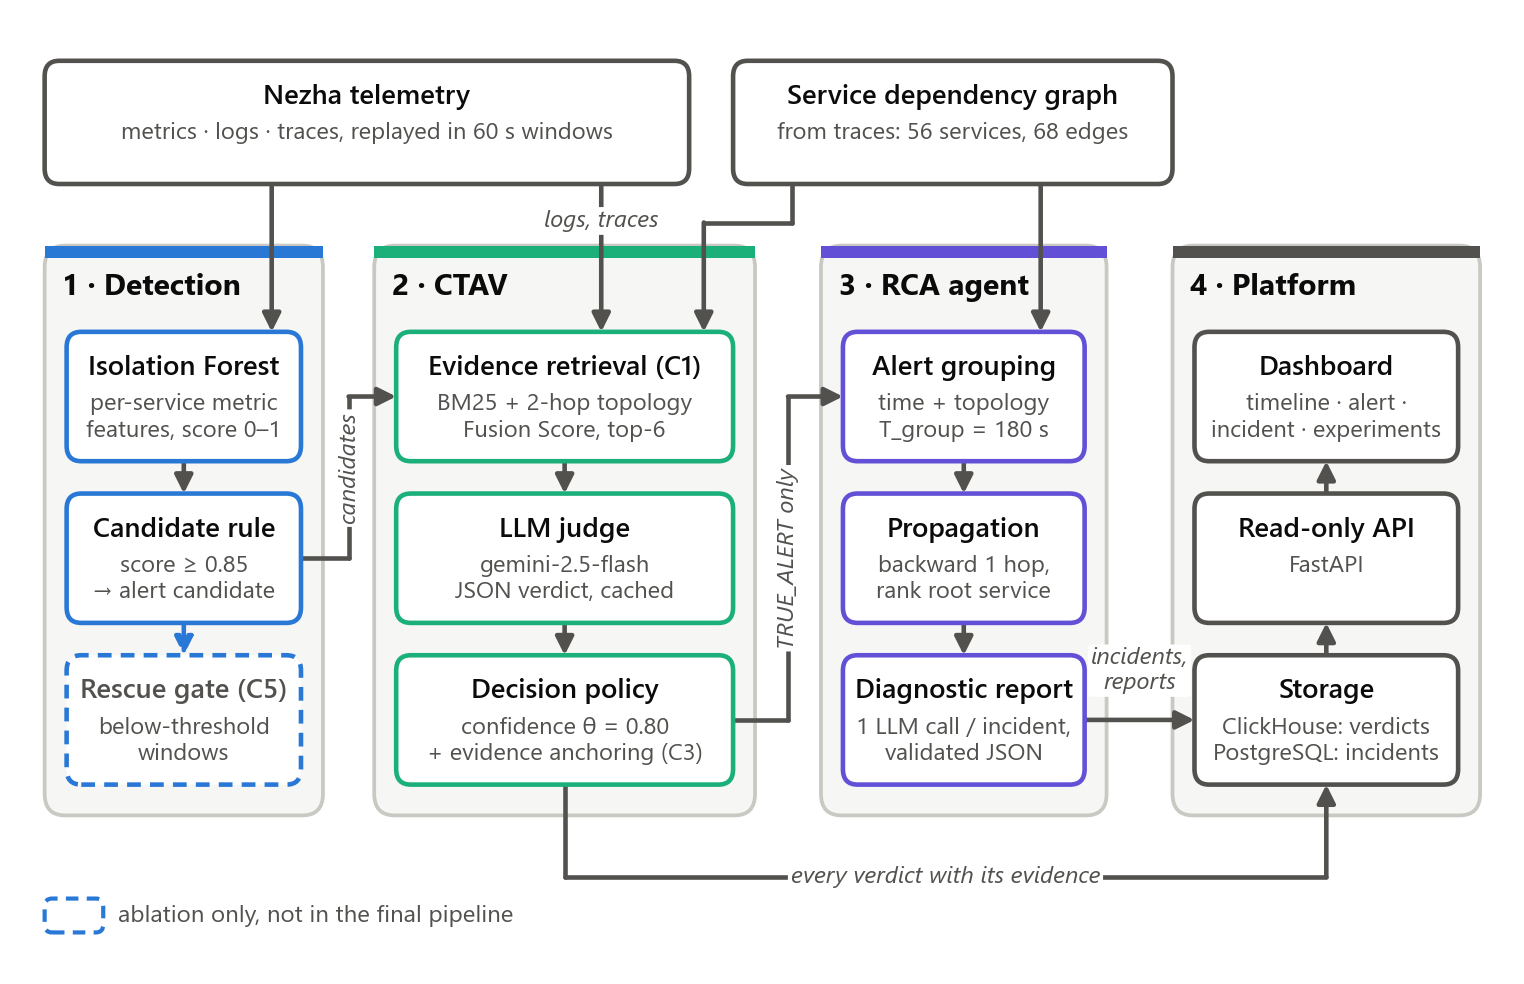
\includegraphics[width=\linewidth]{Images/C1/figures/ch4/h4.1-architecture.png}
  \vspace{0.35cm}
  \caption[Kiến trúc tổng thể bốn khâu của nền tảng ở cấu hình chốt]{Kiến trúc tổng thể bốn khâu ở cấu hình chốt: phát hiện bất thường, \CTAV{}, tác tử \term{RCA}{RCA} và platform (khối nét đứt \comp{C5} chỉ dùng cho ablation). \emph{(Nguồn: tác giả vẽ, có hỗ trợ AI.)}}
  \label{fig:ch4-arch}
\end{figure}

Để bảo đảm khả năng thay thế và kiểm định từng thành phần mà không phá vỡ luồng xử lý, kiến trúc định nghĩa bốn giao diện lõi (\code{Protocol}) cố định ở tầng lược đồ dùng chung, tóm tắt ở Bảng~\ref{tab:ch4-protocols}. Mọi tham số đặc thù của thuật toán (như số bước nhảy đồ thị, hệ số suy giảm thời gian hay ngưỡng tin cậy) đều được nạp qua hàm khởi tạo từ tệp cấu hình YAML thay vì đưa vào chữ ký phương thức. Đối với mô hình ngôn ngữ lớn đóng vai trò bộ thẩm định, kiến trúc chọn một mô hình API cố định duy nhất là \code{gemini-2.5-flash} ở nhiệt độ $0$, đi qua lớp cache bắt buộc và không dùng mô hình cục bộ dự phòng, nhằm loại bỏ sai lệch do đổi mô hình giữa các lượt chạy thực nghiệm và bảo đảm chế độ trình diễn ngoại tuyến hoàn toàn từ cache.

\begin{table}[H]
  \centering
  \caption{Bốn giao diện (\code{Protocol}) lõi và ánh xạ sang các mô-đun hiện thực.}
  \label{tab:ch4-protocols}
  \tblfont
  \tblsetup
  \setlength{\tabcolsep}{4pt}
  \begin{tabularx}{\linewidth}{|l|>{\raggedright\arraybackslash}p{3.0cm}|Y|>{\raggedright\arraybackslash}p{3.7cm}|}
    \hline
    \rowcolor{gray!15}
    \textbf{Protocol} & \textbf{Phương thức chính} & \textbf{Đầu vào / Đầu ra} & \textbf{Thành phần hiện thực} \\
    \hline
    \code{SourceAdapter} & \code{stream()} & Nguồn dữ liệu $\to$ luồng \code{TelemetryWindow} 60~s theo watermark & Bộ phát lại dữ liệu Nezha \\
    \hline
    \code{Detector} & \code{score()}, \code{is\_candidate()} & \code{TelemetryWindow} $\to$ điểm bất thường $[0, 1]$ và cờ ứng viên & Bộ phát hiện Isolation Forest \\
    \hline
    \code{RetrievalStrategy} & \code{retrieve(\allowbreak candidate, budget)} & \code{AlertCandidate}, \code{RetrievalBudget} $\to$ \code{RetrievalResult} & Truy xuất \term{BM25}{BM25} cục bộ, \comp{C1} lai đồ thị và đối chứng không ngữ cảnh \\
    \hline
    \code{Judge} & \code{evaluate(\allowbreak candidate, context)} & \code{AlertCandidate}, \code{RetrievalResult} $\to$ \code{JudgedAlert} & Bộ thẩm định LLM qua cache bất biến \\
    \hline
  \end{tabularx}
\end{table}

\subsubsection{Các vấn đề nghiên cứu}
\label{sec:ch4-van-de}

Xét một hệ microservice được biểu diễn bởi đồ thị phụ thuộc có hướng $G = (V, E)$, trong đó tập đỉnh $V$ là các service và cạnh có hướng $(u, v) \in E$ biểu thị service $u$ gọi service $v$ quan sát được từ cặp \code{SpanID}--\code{ParentID} trong trace. Dữ liệu quan sát đa phương thức được cắt thành các cửa sổ không chồng lấn $w$ có độ dài $60\,\text{s}$, mỗi cửa sổ gắn với một service $s_0 \in V$, pod tương ứng và mốc trung điểm $t_0$. Nhãn thực tế $y(w) \in \{\text{fault}, \text{normal}\}$ được gán theo thời gian thực (\emph{wall-clock}) quanh thời điểm tiêm lỗi như định nghĩa ở Mục~\ref{sec:ch2-du-lieu}.

\textbf{Bài toán nhánh A (Thẩm định cảnh báo dưới ngân sách LLM).} Từ luồng cửa sổ telemetry, bộ phát hiện sinh tập cảnh báo ứng viên $c = (w, s_0, t_0, \text{score}_{\text{det}}, \text{source})$ với $\text{source} \in \{\text{metric}, \text{rescue}\}$. Với mỗi ứng viên $c$, chiến lược truy xuất chọn tập bằng chứng $E(w)$ gồm tối đa $k$ sự kiện log/trace trong ngân sách token định trước, rồi bộ thẩm định kết hợp chính sách quyết định ánh xạ $(w, E(w))$ sang nhãn phán quyết cuối:
\begin{equation}
  \hat{y}(w) \in \{\code{TRUE\_ALERT},\; \code{FALSE\_POSITIVE},\; \code{UNCERTAIN}\},
  \label{eq:ch4-verdict-space}
\end{equation}
kèm điểm tin cậy $p(w) \in [0, 1]$ và tập định danh bằng chứng trích dẫn $C(w) \subseteq E(w)$. Dưới ràng buộc tổng số lần gọi LLM không vượt quá ngân sách $B$, mục tiêu tối ưu của \CTAV{} là giữ được mức tăng thu hồi (Recall) nhờ ngữ cảnh topology của \comp{C1} so với truy xuất cục bộ \term{BM25}{BM25} mà không làm tăng tỷ lệ báo động giả (\term{FPR}{FPR}), tức đồng thời thỏa:
\begin{equation}
  \Delta\text{F1}(\text{\CTAV} - \text{BM25}) > 0, \;
  \Delta\text{FPR}(\text{\CTAV} - \text{BM25}) \le 0, \;
  \Delta\text{Recall}(\text{\CTAV} - \text{C1}) \ge -\delta,
  \label{eq:ch4-ctav-objective}
\end{equation}
với biên chấp nhận giảm thu hồi $\delta = 0{,}05$ đã đăng ký trước cho giả thuyết chính \hyp{H2} (Mục~\ref{sec:ch5-hypotheses}).

\textbf{Bài toán nhánh B (Phân tích nguyên nhân gốc).} Cho tập các cảnh báo đã được \CTAV{} xác nhận $A_{\text{conf}} = \{c \mid \hat{y}(w_c) = \code{TRUE\_ALERT}\}$ và đồ thị phụ thuộc $G$, tác tử \term{RCA}{RCA} cần thực hiện hai ánh xạ nối tiếp: (i) phân hoạch $A_{\text{conf}}$ thành các sự cố $I_1, I_2, \dots, I_m$ theo độ gần thời gian và tính liên thông topology để giảm tải cảnh báo (đo bằng \emph{Alert Reduction Ratio}, \term{ARR}{ARR}); và (ii) với mỗi sự cố $I$, xếp hạng danh sách service nghi vấn gốc $\hat{r}(I) = (v_1, v_2, \dots)$ (đo bằng $\text{Hit}@1$, $\text{Hit}@3$) rồi sinh báo cáo chẩn đoán JSON hợp lệ kèm bằng chứng trích dẫn. Hai bài toán này gắn trực tiếp với năm câu hỏi nghiên cứu ở Chương~\ref{ch:mo-dau}: \rqref{RQ1} kiểm chứng hiện tượng đánh đổi của truy xuất topology và cơ chế \term{ConfirmationBias}{thiên lệch xác nhận}; \rqref{RQ2} và \rqref{RQ3} đánh giá hiệu quả tổng thể và đóng góp riêng lẻ của từng thành phần \comp{C1}--\comp{C5} trong \CTAV{}; \rqref{RQ4} khảo sát độ bền của \CTAV{} theo ngân sách lời gọi $B$; và \rqref{RQ5} đánh giá khả năng định vị gốc cùng chất lượng báo cáo của tác tử \term{RCA}{RCA}. Các ký hiệu chính dùng trong toàn bộ Chương~\ref{ch:de-xuat} được hệ thống hóa trong Bảng~\ref{tab:ch4-ky-hieu}.

\begin{table}[H]
  \centering
  \caption{Bảng ký hiệu toán học dùng trong phát biểu bài toán và thiết kế thuật toán.}
  \label{tab:ch4-ky-hieu}
  \tblfont
  \tblsetup
  \begin{tabularx}{\linewidth}{|l|Y|l|}
    \hline
    \rowcolor{gray!15}
    \textbf{Ký hiệu} & \textbf{Ý nghĩa} & \textbf{Giá trị / Miền} \\
    \hline
    $w,\; s_0,\; t_0$ & Cửa sổ telemetry 60~s, service phát cảnh báo và mốc trung điểm của cửa sổ & $s_0 \in V$ \\
    \hline
    $G = (V, E),\; d_G(u, v)$ & Đồ thị phụ thuộc service từ trace và khoảng cách bước nhảy vô hướng & $56$ nút, $68$ cạnh \\
    \hline
    $E(w),\; C(w)$ & Tập bằng chứng truy xuất (tối đa $k = 6$) và tập bằng chứng judge trích dẫn & $C(w) \subseteq E(w)$ \\
    \hline
    $\alpha, \beta, \gamma,\; \tau_F$ & Trọng số và hằng số suy giảm thời gian của \term{FusionScore}{Fusion Score} (\comp{C1}) & $0{,}35;\; 0{,}25;\; 0{,}40;\; 300\,\text{s}$ \\
    \hline
    $\theta_{\text{local}},\; \theta_{\text{topo}}$ & Ngưỡng tin cậy của chính sách quyết định (\comp{C2} dùng $\theta_{\text{topo}}$, đã loại) & $0{,}80$ ($0{,}85$ cho \comp{C2}) \\
    \hline
    $\eta_1, \eta_2, \eta_3,\; \tau$ & Trọng số ba thành phần và ngưỡng kích hoạt của \term{RescueScore}{Rescue Score} (\comp{C5}) & $(0;\, 0{,}4;\, 0{,}6)$;\; $\tau = 0{,}8$ \\
    \hline
    $T_{\text{group}}$ & Cửa sổ cắt cụm thời gian liên kết đơn khi gom cảnh báo thành sự cố & $180\,\text{s}$ \\
    \hline
    $B$ & Ngân sách tối đa số lần gọi API LLM trong một lượt chạy thẩm định & $\{120, \dots, \text{đủ}\}$ \\
    \hline
  \end{tabularx}
\end{table}

\subsubsection{Các thách thức và khó khăn}
\label{sec:ch4-thach-thuc}

Hiện thực hóa mục tiêu~\eqref{eq:ch4-ctav-objective} cùng nhánh \term{RCA}{RCA} trên dữ liệu quan sát thực tế đối mặt với năm thách thức thiết kế chính:
\begin{enumerate}
  \item \textbf{T1 — Cân bằng \term{FPR}{FPR} và Recall:} Chính sách chặn báo động giả quá chặt dễ hạ nhầm các lỗi thiếu log tường minh (như trễ mạng); \CTAV{} kiểm soát đánh đổi này bằng cặp \comp{C1} + \comp{C3} và ghi nhận minh bạch mức giảm recall ở Chương~\ref{ch:thuc-nghiem}.
  \item \textbf{T2 — Cơ chế thiên lệch khác giả thuyết trực giác:} Phân tích \hyp{H1} trên \splitname{val} (Mục~\ref{sec:ch5-h1}) cho thấy báo động giả không đến từ nhiễu lân cận như giả định tiền đề~\cite{icaetm2026}, mà từ \term{ConfirmationBias}{thiên lệch xác nhận}~\cite{sharma2024sycophancy} trên trace span cục bộ sát $t_0$, buộc thiết kế chuyển từ lọc khoảng cách đồ thị (\comp{C2}) sang kiểm tra tính bất thường định lượng tại chính $s_0$ (\comp{C3}).
  \item \textbf{T3 — Giới hạn ngân sách và tái lập:} Hệ thống dùng cache bất biến khóa \code{sha256} và tách chính sách quyết định thành hàm thuần trên phán quyết đã lưu cache để chạy ablation với $0$ lượt gọi mới.
  \item \textbf{T4 — Cảnh báo đầu vào thưa ở tầng \term{RCA}{RCA}:} Sau khi \CTAV{} lọc mạnh FP, chuỗi cảnh báo sang \term{RCA}{RCA} thường thưa; tác tử \term{RCA}{RCA} tách tầng thuật toán tất định khỏi tầng tóm tắt LLM có kiểm duyệt để dễ cô lập nguyên nhân sai (Mục~\ref{sec:ch5-rca}).
  \item \textbf{T5 — Kỷ luật chống rò rỉ:} Chia split theo \code{injection\_id} kèm vùng đệm $600\,\text{s}$, đăng ký trước \hyp{H0}--\hyp{H5} và đóng băng cấu hình trước khi chạy \splitname{test} đúng một lần.
\end{enumerate}

% -----------------------------------------------------------------------------
\subsection{Isolation Forest và cổng Rescue (\comp{C5})}
\label{sec:ch4-detector}

Mục này trình bày tầng đầu tiên của pipeline: bộ phát hiện bất thường chuỗi thời gian Isolation Forest tạo tập ứng viên cho \CTAV{}, cùng cơ chế cổng cứu cảnh báo \comp{C5} (\code{Rescue Score}) dùng để kiểm chứng khả năng thu hồi các cửa sổ bị bộ phát hiện metric bỏ sót.

\textbf{Vấn đề giải quyết.} Trên tập dữ liệu Nezha~\cite{nezha} gồm hàng chục nghìn cửa sổ 60~s với tỷ lệ mất cân bằng xấp xỉ $1:135$ giữa cửa sổ lỗi và cửa sổ bình thường, gọi trực tiếp LLM trên mọi cửa sổ là bất khả thi về chi phí lẫn độ trễ. Tầng phát hiện cần một mô hình không giám sát chạy nhanh, chỉ huấn luyện trên tập \splitname{dev} để loại bỏ phần lớn cửa sổ bình thường mà vẫn đưa đủ cửa sổ bất thường vào hàng đợi thẩm định. Ngược lại, một số dạng lỗi ứng dụng (như ngoại lệ phần mềm hoặc lỗi trả về sớm) ít gây biến động mạnh trên metric hạ tầng, đặt ra câu hỏi liệu có thể cứu lại những cửa sổ dưới ngưỡng metric bằng dấu hiệu log và đồ thị phụ thuộc hay không.

\textbf{Thiết kế bộ phát hiện Isolation Forest.} Bộ phát hiện \code{IsolationForestDetector} duy trì một bộ đệm cuộn (\emph{rolling buffer}) kích thước \code{buffer\_size = 2} riêng cho từng khóa pod (dự phòng theo tên service nếu thiếu pod), tương ứng khoảng $120\,\text{s}$ lịch sử gần nhất. Trên mỗi cửa sổ, với từng metric trong tập đặc trưng của tập huấn luyện, mô-đun trích xuất bảy thống kê: trung bình (\code{mean}), độ lệch chuẩn (\code{std}), giá trị nhỏ nhất (\code{min}), lớn nhất (\code{max}), giá trị cuối (\code{last}), độ chênh (\code{delta}) và tỷ lệ thiếu mẫu (\code{missing\_fraction}). Các metric vắng mặt trong một cửa sổ (ví dụ phân vị độ trễ \code{NaN} khi không có request) được điền bằng giá trị quan sát gần nhất của chính pod đó hoặc trung vị trên tập \splitname{dev} — tuyệt đối không điền $0{,}0$ để tránh biểu diễn nhầm một cửa sổ nhàn rỗi thành độ trễ cực thấp. Điểm bất thường từ Isolation Forest~\cite{isof} được chuẩn hóa theo phân vị trên tập huấn luyện về đoạn $[0, 1]$. Một cửa sổ chỉ trở thành ứng viên \code{AlertCandidate(source="metric")} khi bộ đệm của pod đã đầy (tránh báo động giả lúc khởi động lạnh) và thỏa:
\begin{equation}
  \text{score}_{\text{IF}}(w) \ge 0{,}85.
  \label{eq:ch4-if-rule}
\end{equation}
Ngoài điểm số, bộ phát hiện xuất ba đặc trưng có độ lệch chuẩn lớn nhất so với phân bố huấn luyện (\code{top\_features}) để đưa vào ngữ cảnh của bộ thẩm định LLM.

\textbf{\xtarget{def:C5}Thiết kế cổng cứu cảnh báo \comp{C5} (\code{Rescue Score}).} Với các cửa sổ không vượt ngưỡng~\eqref{eq:ch4-if-rule} ($y_{\text{IF}}(w) = 0$), bộ tính điểm cứu cảnh báo tính tổng trọng số dựa trên ba thành phần chuẩn hóa trong $[0, 1]$:
\begin{equation}
  \text{RescueScore}(w \mid A) = \eta_1 \Lambda_{\text{log}}(w) + \eta_2 \Phi_{\text{topo}}(w, A) + \eta_3 \Delta_{\text{time}}(w, A),
  \label{eq:ch4-rescue}
\end{equation}
với $\eta_1, \eta_2, \eta_3 \ge 0$ và $\eta_1 + \eta_2 + \eta_3 = 1$, trong đó:
\begin{align}
  \Lambda_{\text{log}}(w) &= 1 - \exp\!\left(-\frac{N_{\text{err}}(w)}{k_{\text{log}}}\right), \label{eq:ch4-rescue-log} \\
  \Phi_{\text{topo}}(w, A) &= \max_{a \in A} \frac{1}{1 + d_G(s_w, s_a)}, \label{eq:ch4-rescue-topo} \\
  \Delta_{\text{time}}(w, A) &= \max_{a \in A} \exp\!\left(-\frac{|t_w - t_a|}{\sigma}\right). \label{eq:ch4-rescue-time}
\end{align}
Ở đây, $N_{\text{err}}(w)$ là số dòng log lỗi của pod trong cửa sổ $w$ khớp mức \code{ERROR}/\code{FATAL}/\code{CRITICAL} hoặc mẫu HTTP 5xx, \code{exception}, \code{panic}, \code{traceback}. Tập $A$ là tập các cảnh báo đã được \CTAV{} xác nhận (không bao giờ dùng nhãn thực tế) thỏa điều kiện nhân quả $t_w - T_{\text{active}} \le t_a \le t_w$, nghĩa là không sử dụng cảnh báo từ tương lai. Nếu $\text{RescueScore}(w \mid A) \ge \tau$, cửa sổ được đẩy vào hàng đợi thẩm định với nhãn \code{source="rescue"}.

\textbf{Tham số, cách chọn và vai trò hiện tại.} Tham số của Isolation Forest và \comp{C5} được tổng hợp chung trong Bảng~\ref{tab:ch4-pipeline-params}. Với \comp{C5}, quét ngoại tuyến $147$ cấu hình trên \splitname{val} chọn $\eta = (0;\, 0{,}4;\, 0{,}6)$ và $\tau = 0{,}8$ (thành phần $\Lambda_{\text{log}}$ bằng $0$ trên hầu hết cửa sổ bị bỏ sót), nhưng khi chạy qua \CTAV{} cổng này không cải thiện F1 có ý nghĩa thống kê. Do đó, \textbf{Isolation Forest là bộ phát hiện chính đang dùng}, còn \textbf{\comp{C5} chỉ giữ vai trò một điểm ablation độc lập}, không bật trong cấu hình cuối (bằng chứng ở Mục~\ref{sec:ch5-c5} và Mục~\ref{sec:ch5-test-c5}).

% -----------------------------------------------------------------------------
\subsection{\CTAV{} — Thẩm định cảnh báo có nhận biết topology và hiệu chỉnh}
\label{sec:ch4-ctav}

Mục này trình bày hạt nhân phương pháp của đề tài: từ tổng quan kiến trúc \CTAV{} và quá trình tinh gọn trên tập \splitname{val}, đến từng thành phần truy xuất, chính sách quyết định, định tuyến và bộ thẩm định LLM.

\subsubsection{Tổng quan \CTAV{}}
\label{sec:ch4-ctav-tong-quan}

Thiết kế ban đầu của \CTAV{} gồm bốn cơ chế phối hợp: tầng 1 truy xuất cục bộ \term{BM25}{BM25}, bộ định tuyến hai tầng thích nghi \textbf{\comp{C4}} chỉ leo thang sang tầng 2 truy xuất topology \textbf{\comp{C1}} khi tầng 1 chưa chắc chắn, ngưỡng tin cậy bất đối xứng theo nguồn bằng chứng \textbf{\comp{C2}} ($\theta_{\text{topo}} > \theta_{\text{local}}$) và quy tắc neo bằng chứng bất thường \textbf{\comp{C3}}. Hình~\ref{fig:ch4-ctav-compare} đối chiếu trực tiếp thiết kế ban đầu (a) với cấu hình chốt (b) sau kiểm định loại trừ trên tập \splitname{val}; người đọc cần chú ý các khối nét đứt bị lược bỏ ở cấu hình cuối nhưng vẫn giữ trong mã nguồn để phục vụ thí nghiệm loại trừ \hyp{H3}.

\begin{figure}[htbp]
  \centering
  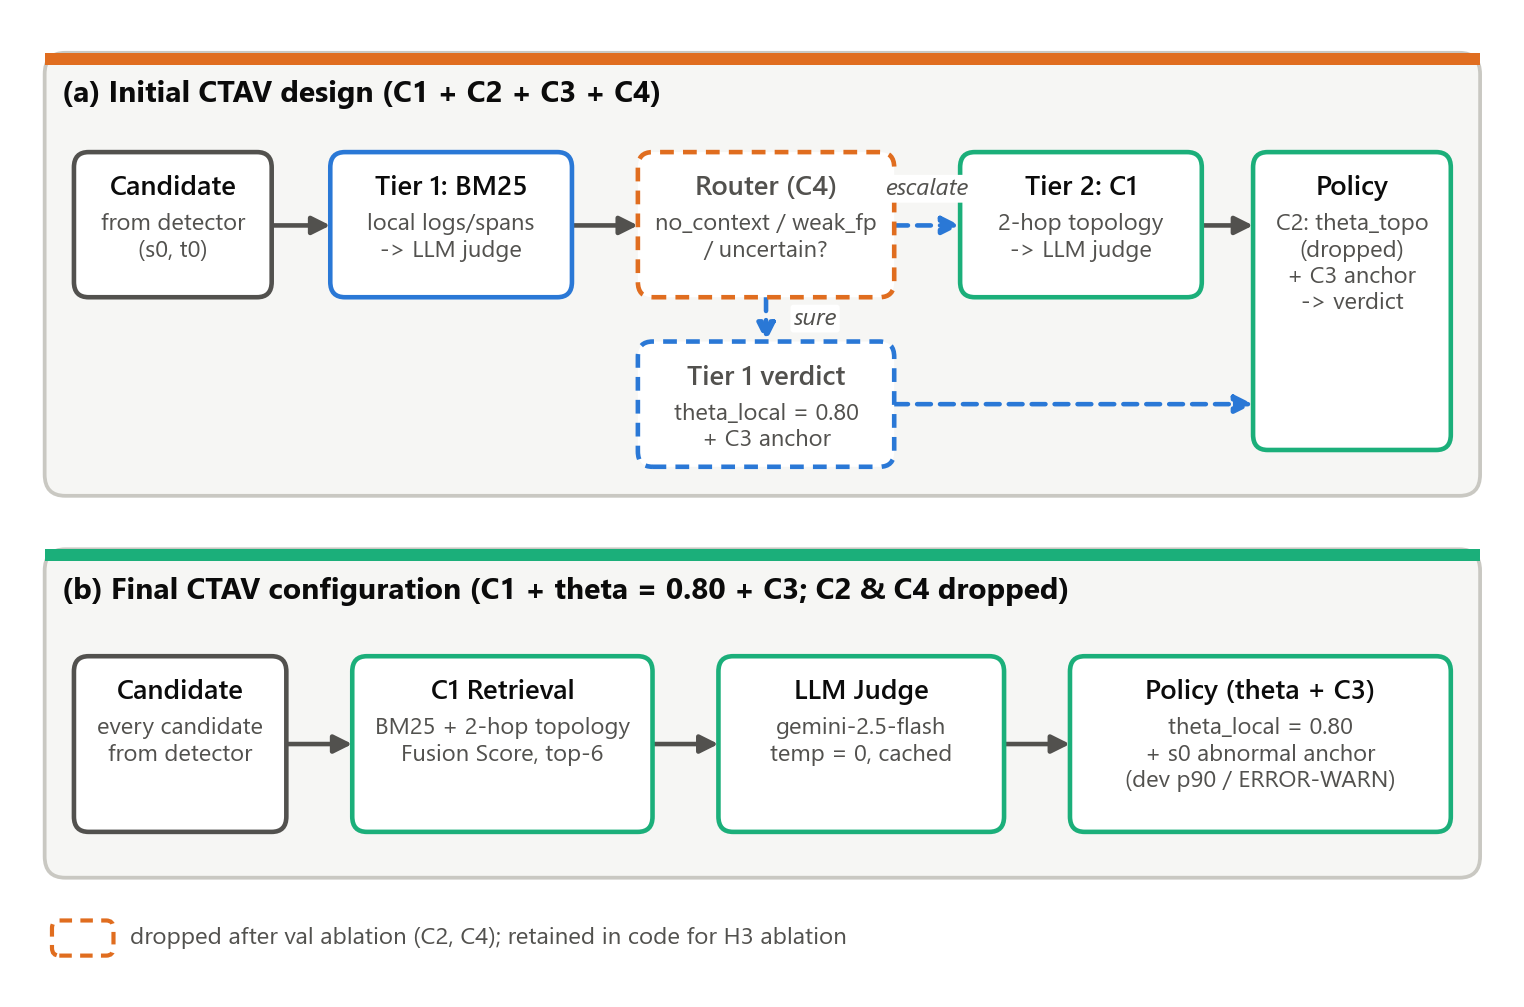
\includegraphics[width=\linewidth]{Images/C1/figures/ch4/h4.4-ctav-design-vs-final.png}
  \vspace{0.35cm}
  \caption[So sánh kiến trúc CTAV ban đầu và cấu hình chốt]{So sánh kiến trúc \CTAV{} giữa thiết kế ban đầu (a) và cấu hình chốt (b) chỉ giữ \comp{C1}, ngưỡng $\theta_{\text{local}} = 0{,}80$ và neo bằng chứng \comp{C3} (\comp{C2}, \comp{C4} đã loại). \emph{(Nguồn: tác giả vẽ, có hỗ trợ AI.)}}
  \label{fig:ch4-ctav-compare}
\end{figure}

Trên tập \splitname{val}, kiểm định loại trừ dẫn đến hai quyết định tinh gọn: loại \comp{C4} vì chạy hai tầng tốn chi phí hơn chạy thẳng \comp{C1} mà F1 không tăng, và loại \comp{C2} vì bỏ \comp{C2} không làm thay đổi đáng kể \term{FPR}{FPR} (Mục~\ref{sec:ch5-val-ctav}). Cấu hình chốt của \CTAV{} vì thế rút gọn thành: \emph{mọi ứng viên $\to$ truy xuất \comp{C1} $\to$ judge \code{gemini-2.5-flash} $\to$ ngưỡng $\theta_{\text{local}} = 0{,}80$ $\to$ neo bằng chứng \comp{C3} (ngưỡng nền \splitname{dev} $p_{90}$)}. Vai trò cố định của năm thành phần \comp{C1}--\comp{C5} được tổng kết ở Bảng~\ref{tab:ch4-c1-c5}.

\begin{table}[H]
  \centering
  \caption{Vai trò hiện tại của từng thành phần trong không gian thiết kế \CTAV{} và cổng cứu cảnh báo.}
  \label{tab:ch4-c1-c5}
  \tblfont
  \tblsetup
  \begin{tabularx}{\linewidth}{|l|Y|>{\raggedright\arraybackslash}p{2.7cm}|Y|}
    \hline
    \rowcolor{gray!15}
    \textbf{Ký hiệu} & \textbf{Chức năng} & \textbf{Vai trò hiện tại} & \textbf{Cơ sở quyết định trên \splitname{val}} \\
    \hline
    \textbf{\comp{C1}} & Truy xuất lai \term{BM25}{BM25}--topology (\term{FusionScore}{Fusion Score}) & \textbf{Đang dùng} & Tái lập lợi ích nhận diện của topology trên mọi ứng viên \\
    \hline
    \textbf{\comp{C2}} & Ngưỡng bất đối xứng theo nguồn bằng chứng ($\theta_{\text{topo}} > \theta_{\text{local}}$) & \textbf{Đã loại} & Bỏ \comp{C2} chỉ thêm 2 FP ($\Delta\text{FPR}$ CI chạm $0$) \\
    \hline
    \textbf{\comp{C3}} & Neo bằng chứng bất thường của $s_0$ (ngưỡng nền \splitname{dev} $p_{90}$) & \textbf{Đang dùng} (đóng góp chính) & Hạ mạnh FP của \comp{C1} ($606 \to 51$), tăng F1 có ý nghĩa \\
    \hline
    \textbf{\comp{C4}} & Định tuyến hai tầng thích nghi (\term{BM25}{BM25} $\to$ \comp{C1}) & \textbf{Đã loại} & Chi phí cao hơn \comp{C1} chạy thẳng ($5{,}14$ vs $3{,}28$ USD), F1 không tăng \\
    \hline
    \textbf{\comp{C5}} & Cổng cứu cảnh báo \code{Rescue Score} & \textbf{Chỉ là ablation} & Thêm 2 TP / 16 FP ($\Delta\text{F1} = +0{,}001$, CI chứa $0$) \\
    \hline
  \end{tabularx}
\end{table}

\subsubsection{\term{BM25}{BM25} cục bộ và bộ thẩm định nền}
\label{sec:ch4-bm25}

\textbf{Vấn đề giải quyết và thiết kế.} Để đối chứng đóng góp thực chất của truy xuất topology và chính sách hiệu chỉnh trên cùng tập ứng viên, mô hình judge và ngân sách $B$, hệ thống hiện thực hai chiến lược nền song song với \comp{C1} (\code{hybrid\_bm25\_graph}): (i)~\code{bm25\_hybrid} dựng truy vấn từ tên service $s_0$, ba \code{top\_features} và từ khóa lỗi chuẩn hóa (tuyệt đối không đưa nhãn lỗi vào truy vấn), tìm riêng trong log và trace span của $s_0$ trong biên $\pm 8$ phút, xếp hạng bằng \term{BM25}{BM25}~\cite{robertson2009bm25} chọn top $k = 6$ trong $4.000$ token; và (ii)~\code{no\_retrieval} trả ngữ cảnh rỗng ($E(w) = \emptyset$, tắt \code{require\_evidence}) để đo năng lực suy luận chỉ từ ảnh chụp metric ở cùng ngân sách $B$. Các biến thể ablation thời gian thuần ($\beta = 1$) hoặc đồ thị thuần ($\gamma = 1$) được cấu hình trực tiếp qua trọng số của \comp{C1} thay vì tạo lớp riêng.

\textbf{Vai trò và dẫn chiếu.} \code{bm25\_hybrid} là baseline khoa học cho \hyp{H0}, \hyp{H2} và tầng 1 của nhánh loại trừ \comp{C4}; \code{no\_retrieval} là baseline không \term{RAG}{RAG} cho \hyp{H4} (kết quả ở Mục~\ref{sec:ch5-val}, \ref{sec:ch5-test} và \ref{sec:ch5-budget}).

\subsubsection{Truy xuất nhận biết topology \comp{C1}}
\label{sec:ch4-c1}\xtarget{def:C1}

\textbf{Vấn đề giải quyết.} Khi sự cố lan truyền qua nhiều microservice, bằng chứng trực tiếp trong cửa sổ của $s_0$ có thể thưa hoặc chỉ thể hiện độ trễ tăng, trong khi lỗi gốc xuất hiện rõ ở service được gọi hoặc ở các sự kiện diễn ra sát $t_0$ nhưng ít trùng khớp từ khóa với truy vấn metric. Thành phần \textbf{\comp{C1}} (bộ truy xuất lai từ khóa--đồ thị \code{HybridBm25GraphRetriever}) mở rộng phạm vi truy xuất theo đồ thị phụ thuộc và kết hợp ba tín hiệu từ khóa, thời gian và khoảng cách đồ thị.

\textbf{Thiết kế.} Quá trình truy xuất của \comp{C1} được minh họa trên Hình~\ref{fig:ch4-c1}, tách thành hai bước độc lập là dựng bể ứng viên (\code{build\_pool}) và xếp hạng chọn lọc (\code{top\_events}) nhằm cho phép đánh giá lại nhiều bộ trọng số trên cùng một bể mà không lặp lại bước truy vấn dữ liệu. Cụ thể:
\begin{enumerate}
  \item \emph{Mở rộng vùng lân cận 2 hop:} Từ $s_0$, tìm tập service có thể tới được trong bán kính $d_G(s_i, s_0) \le 2$ trên đồ thị phụ thuộc vô hướng ($56$ service, $68$ cạnh), trong đó $d_G(s_0, s_0) = 0$. Kho dữ liệu được lọc trong khung thời gian $[t_{\text{start}} - 8\,\text{phút},\; t_{\text{end}} + 8\,\text{phút}]$ (\code{bm25\_pool = window}; chế độ \code{global} không giới hạn thời gian chỉ giữ riêng cho bước kiểm chứng hồi quy G-paper).
  \item \emph{Hợp nhất hai nguồn ứng viên:} Lấy top \code{bm25\_k = 60} sự kiện có điểm \term{BM25}{BM25} cao nhất trên kho vùng lân cận, hợp nhất và khử trùng lặp với tối đa $20$ sự kiện gần trung điểm $t_0$ nhất của mỗi service trong bán kính 2 hop. Mỗi sự kiện gắn nhãn nguồn gốc \code{origin = local} nếu $d_G = 0$, ngược lại \code{graph}.
  \item \emph{Xếp hạng \term{FusionScore}{Fusion Score} và cắt theo ngân sách:} Mỗi sự kiện $e_i = (s_i, t_i)$ trong bể ứng viên được chấm điểm hợp nhất:
  \begin{equation}
    \text{Score}(e_i, s_0, t_0) = \alpha \cdot \widehat{\text{BM25}}(e_i) + \beta \cdot \exp\!\left(-\frac{|t_i - t_0|}{\tau_F}\right) + \gamma \cdot \frac{1}{1 + d_G(s_i, s_0)},
    \label{eq:ch4-fusion}
  \end{equation}
  với $\alpha + \beta + \gamma = 1$, $\widehat{\text{BM25}}(e_i)$ là điểm \term{BM25}{BM25} chuẩn hóa min--max trên toàn bể ứng viên (bằng $1$ nếu điểm dương trên bể đồng nhất, bằng $0$ nếu điểm bằng $0$), và $\text{GraphSim} = 0$ nếu service không liên thông. Sau khi xếp hạng, hệ thống chọn top $k = 6$ sự kiện không vượt quá $4.000$ token. Tùy chọn hạn ngạch \code{k\_graph} (biến thể \comp{C1}-quota) cho phép giữ tối thiểu $\min(k_{\text{graph}}, \text{số sự kiện sẵn có})$ sự kiện \code{origin = graph}; engine vector hóa \code{WindowIndex} tăng tốc truy vấn gấp khoảng 10 lần mà cho đầu ra trùng khớp tuyệt đối với bản tham chiếu Python thuần.
\end{enumerate}

\begin{figure}[htbp]
  \centering
  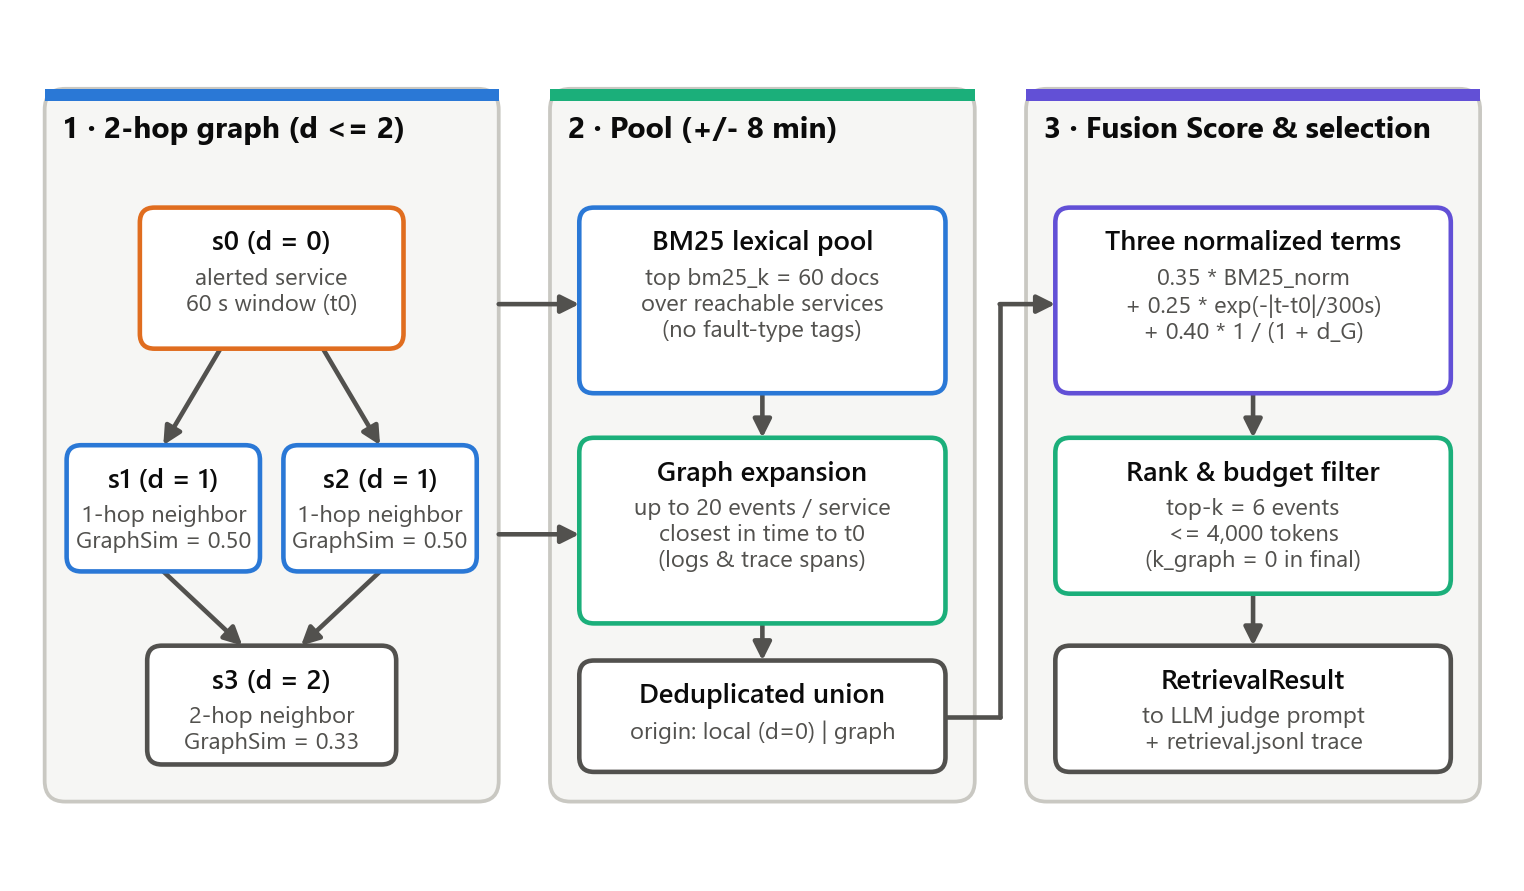
\includegraphics[width=\linewidth]{Images/C1/figures/ch4/h4.5-c1-2hop-fusion.png}
  \vspace{0.35cm}
  \caption[Cơ chế truy xuất nhận biết topology C1 và Fusion Score]{Cơ chế truy xuất nhận biết topology \comp{C1}: mở rộng 2~hop quanh $s_0$, hợp nhất bể \term{BM25}{BM25} và đồ thị ($\pm 8$~phút), xếp hạng \term{FusionScore}{Fusion Score} chọn top-6. \emph{(Nguồn: tác giả vẽ, có hỗ trợ AI.)}}
  \label{fig:ch4-c1}
\end{figure}

\textbf{Tham số, cách chọn và vai trò hiện tại.} Các tham số của \comp{C1} được tổng hợp trong Bảng~\ref{tab:ch4-pipeline-params}. Sau khi khảo sát hạn ngạch $k_{\text{graph}} \in \{0, 1, 2, 3\}$ và 32 tổ hợp trọng số trên \splitname{val} (Mục~\ref{sec:ch5-val-c1}), cấu hình chốt giữ $(\alpha, \beta, \gamma) = (0{,}35;\, 0{,}25;\, 0{,}40)$, $\tau_F = 300\,\text{s}$ và \code{k\_graph = 0} vì ép thêm bằng chứng lân cận không cải thiện độ trúng gốc hay F1. \textbf{\comp{C1} đang dùng} làm chiến lược truy xuất duy nhất của \CTAV{} (bằng chứng ở Mục~\ref{sec:ch5-val} và Mục~\ref{sec:ch5-test}).

\subsubsection{Chính sách quyết định: neo bằng chứng (\comp{C3}) và ngưỡng bất đối xứng (\comp{C2}, đã loại)}
\label{sec:ch4-policy}

\textbf{Vấn đề giải quyết.} Khi đưa ngữ cảnh từ \comp{C1} vào \emph{LLM-as-a-Judge}, mô hình ngôn ngữ có xu hướng xác nhận \code{TRUE\_ALERT} với điểm tin cậy cao ($0{,}85$--$0{,}90$) ngay cả trên các cửa sổ bình thường chỉ vì thấy các trace span nằm sát mốc $t_0$ (khảo sát \hyp{H1} trên \splitname{val}, Mục~\ref{sec:ch5-h1}). Thay vì chỉ dựa vào nhãn thô hoặc câu nhắc prompt vốn khó kiểm soát độ ổn định, tầng chính sách quyết định đặt các quy tắc định lượng tường minh sau bộ thẩm định để chặn báo động giả có hệ thống.

\textbf{Thiết kế chính sách quyết định.} Như minh họa trên Hình~\ref{fig:ch4-policy}, chính sách là một \emph{hàm thuần} nhận phán quyết thô \code{raw\_verdict}, độ tin cậy \code{confidence} và tập thông tin bằng chứng đã trích dẫn \code{cited} của từng ứng viên đã lưu cache. Mọi phán quyết thô khác \code{TRUE\_ALERT} (tức \code{FALSE\_POSITIVE}, \code{UNCERTAIN} hoặc lỗi \code{manual\_review}) đi thẳng không đổi; riêng \code{TRUE\_ALERT} phải vượt qua tuần tự ba cổng:
\begin{enumerate}
  \item \emph{Cổng kiểm tra trích dẫn (\code{require\_evidence}):} Tập \code{cited} (sau khi đã lọc bỏ mọi \code{event\_id} không tồn tại trong ngữ cảnh) phải khác rỗng; nếu rỗng thì hạ xuống \code{UNCERTAIN} với cờ \code{downgraded\_by\_evidence\_rule}.
  \item \xtarget{def:C2}\emph{Cổng ngưỡng tin cậy (và nhánh \comp{C2} đã loại):} Nếu $\text{confidence} < \theta_{\text{local}}$ ($\theta_{\text{local}} = 0{,}80$), hạ xuống \code{UNCERTAIN} (\code{downgraded\_by\_threshold}). Trong thiết kế ban đầu có bật \textbf{\comp{C2}}, các phán quyết xuất phát từ tầng topology ($tier = 2$) phải vượt ngưỡng cao hơn $\theta_{\text{topo}} = 0{,}85$; nếu $\theta_{\text{local}} \le \text{confidence} < \theta_{\text{topo}}$ thì hạ với cờ \code{downgraded\_by\_gating}.
  \item \xtarget{def:C3}\emph{Cổng neo bằng chứng bất thường (\textbf{\comp{C3}}):} Phán quyết \code{TRUE\_ALERT} chỉ được giữ khi tồn tại ít nhất một sự kiện $e \in C(w)$ thỏa vị từ bất thường của chính service phát cảnh báo $s_0$:
  \begin{equation}
    \begin{aligned}
      \text{Abnormal}(e, s_0) \iff (s_e = s_0) \land \Big[
        &\big(e \text{ là log} \land \text{level}(e) \in \{\code{ERROR}, \code{WARN}\}\big) \\
        &\lor \big(e \text{ là span} \land \text{dur}(e) > q_{90}(s_0, \text{op}_e)\big)
      \Big],
    \end{aligned}
    \label{eq:ch4-c3-anchor}
  \end{equation}
  trong đó $q_{90}(s_0, \text{op}_e)$ là phân vị thứ 90 của thời lượng \code{duration\_ms} cho cặp $(s_0, \text{op}_e)$ ước lượng từ bộ tính ngưỡng nền span. Nếu không có sự kiện nào thỏa~\eqref{eq:ch4-c3-anchor}, cảnh báo bị hạ xuống \code{UNCERTAIN} với cờ \code{downgraded\_by\_anchoring}.
\end{enumerate}

\begin{figure}[htbp]
  \centering
  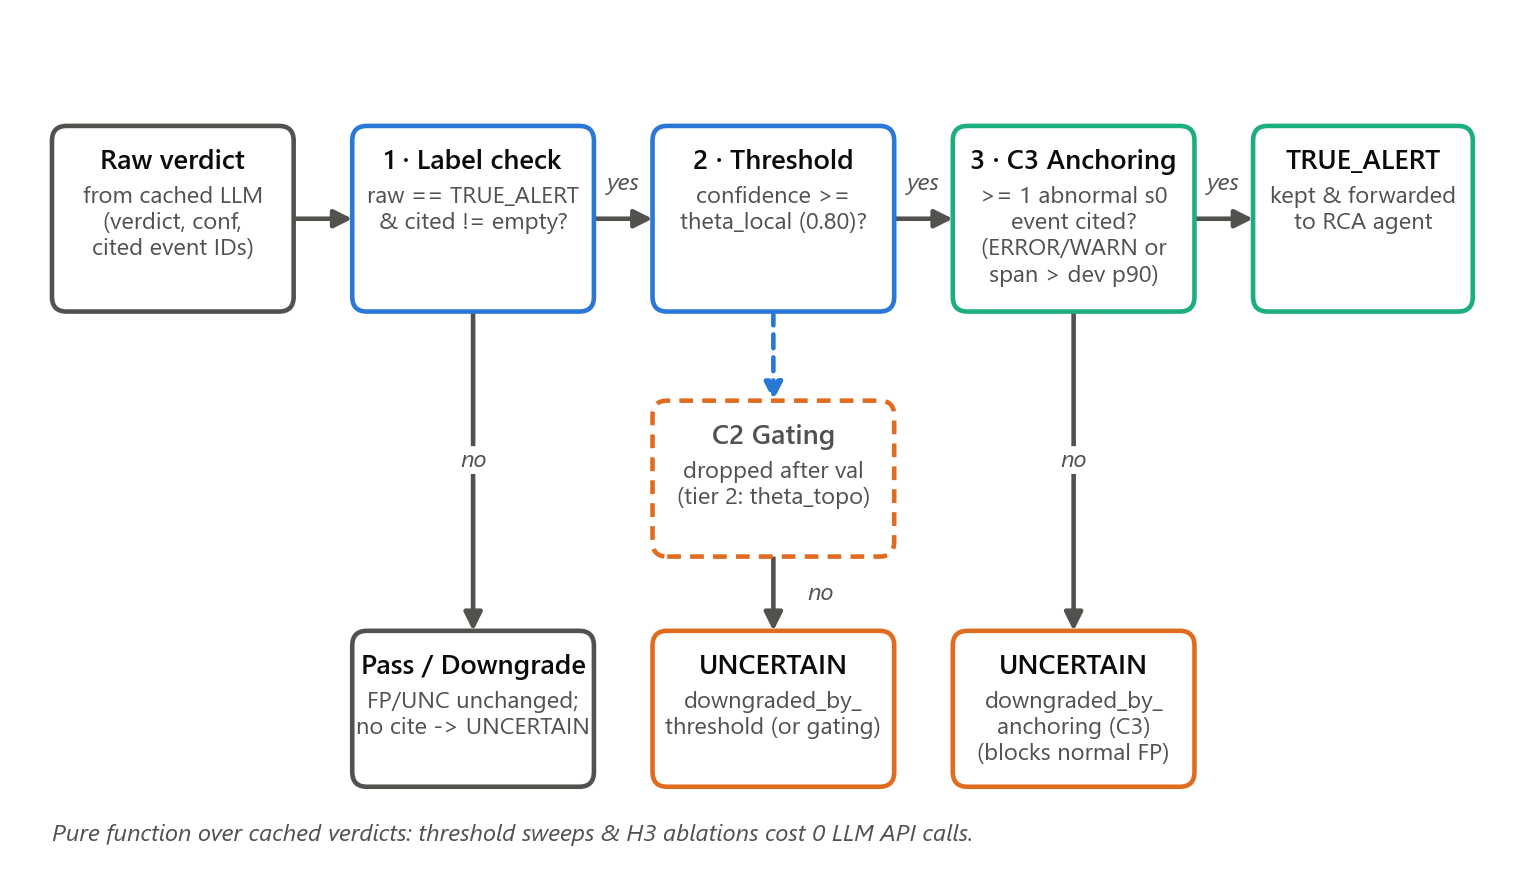
\includegraphics[width=\linewidth]{Images/C1/figures/ch4/h4.6-decision-policy.png}
  \vspace{0.35cm}
  \caption[Sơ đồ luồng chính sách quyết định CTAV]{Sơ đồ luồng chính sách quyết định \CTAV{} trên phán quyết đã lưu cache: kiểm trích dẫn, ngưỡng $\theta_{\text{local}} = 0{,}80$ (\comp{C2} nét đứt đã loại) và neo \comp{C3} tại $s_0$. \emph{(Nguồn: tác giả vẽ, có hỗ trợ AI.)}}
  \label{fig:ch4-policy}
\end{figure}

\textbf{Xây dựng ngưỡng nền và lựa chọn thiết kế.} Để ngưỡng nền $q_{90}(s_0, \text{op}_e)$ không bị nhiễm độ trễ lỗi lan truyền, bộ chọn \code{SpanSelector} chỉ giữ các trace span thuộc cửa sổ bình thường sạch trên \splitname{dev} (ngoài mọi khoảng tiêm lỗi của cùng hệ thống) với tối thiểu $\code{MIN\_SPANS} = 30$ span mỗi cặp $(s_0, \text{op}_e)$; cặp thiếu ngưỡng không thể dùng làm bằng chứng neo. Bảng~\ref{tab:ch4-policy-rules} đối chiếu các điều kiện hạ bậc cùng hai nguồn ngưỡng nền khảo sát trên \splitname{val}: theo quy tắc lựa chọn đã khóa, \CTAV{} chốt ngưỡng nền \splitname{dev} $p_{90}$ và giữ biến thể ngưỡng trượt 60 phút không cần nhãn (\code{RollingSpanBaseline}) làm đối chứng độ nhạy bắt buộc ở Chương~\ref{ch:thuc-nghiem}.

\begin{table}[H]
  \centering
  \caption{Tổng hợp các điều kiện hạ bậc của chính sách quyết định và so sánh hai nguồn ngưỡng nền cho \comp{C3}.}
  \label{tab:ch4-policy-rules}
  \tblfont
  \tblsetup
  \begin{tabularx}{\linewidth}{|>{\raggedright\arraybackslash}p{3.0cm}|Y|Y|>{\raggedright\arraybackslash}p{2.2cm}|}
    \hline
    \rowcolor{gray!15}
    \textbf{Quy tắc / Biến thể} & \textbf{Điều kiện áp dụng} & \textbf{Hành động \& ghi nhận} & \textbf{Trạng thái} \\
    \hline
    \code{require\_\allowbreak evidence} & \code{raw\_verdict == TRUE\_ALERT} nhưng không có ID trích dẫn hợp lệ & Hạ \code{UNCERTAIN} (\code{downgraded\_by\_\allowbreak evidence\_rule}) & Đang dùng \\
    \hline
    Ngưỡng $\theta_{\text{local}}$ & $\text{confidence} < 0{,}80$ & Hạ \code{UNCERTAIN} (\code{downgraded\_by\_\allowbreak threshold}) & Đang dùng \\
    \hline
    Gating \textbf{\comp{C2}} & Tầng topology ($tier = 2$) có $0{,}80 \le \text{confidence} < 0{,}85$ & Hạ \code{UNCERTAIN} (\code{downgraded\_by\_\allowbreak gating}) & \textbf{Đã loại} \\
    \hline
    Neo \textbf{\comp{C3}} (\splitname{dev} $p_{90}$) & Không có log \code{ERROR}/\code{WARN} hay span của $s_0$ vượt $q_{90}$ tính từ \splitname{dev} sạch ($\ge 30$ span) & Hạ \code{UNCERTAIN} (\code{downgraded\_by\_\allowbreak anchoring}); giữ ID neo nếu đạt & \textbf{Đang dùng} (chính) \\
    \hline
    Neo \textbf{\comp{C3}} (trượt 60 phút) & Như trên nhưng tính $q_{90}$ trên cửa sổ trượt $[t_{\text{start}} - g - 60\text{m},\; t_{\text{start}} - g)$ không cần nhãn & Phủ $\approx 93\%$ span nhưng cho F1 thấp hơn trên \splitname{val} & Ablation / độ nhạy \\
    \hline
  \end{tabularx}
\end{table}

\textbf{Vai trò hiện tại và dẫn chiếu.} \textbf{\comp{C3} đang dùng} và là đóng góp quyết định hiệu quả kìm báo động giả của \CTAV{}; \textbf{\comp{C2} đã loại} sau kiểm định \hyp{H3} trên \splitname{val}. Nhờ lưu song song phán quyết thô và phán quyết sau chính sách, mọi lần quét ngưỡng hay phân tích loại trừ đều tiêu tốn $0$ lần gọi API mới. Bằng chứng chi tiết nằm tại Mục~\ref{sec:ch5-val}, Mục~\ref{sec:ch5-test} và Mục~\ref{sec:ch5-ablation}.

\subsubsection{Định tuyến hai tầng thích nghi (\comp{C4}, đã loại)}
\label{sec:ch4-c4}\xtarget{def:C4}

\textbf{Vấn đề giải quyết.} Thành phần định tuyến hai tầng \textbf{\comp{C4}} được thiết kế ban đầu nhằm giảm chi phí gọi LLM của ngữ cảnh topology: chỉ chạy truy xuất cục bộ \term{BM25}{BM25} ở tầng 1 cho mọi ứng viên, và chỉ leo thang sang tầng 2 (\comp{C1}) đối với những ứng viên mà tầng 1 chưa đủ cơ sở kết luận.

\textbf{Thiết kế và tham số.} Hàm \code{route()} chạy tầng 1 (\term{BM25}{BM25} $\to$ judge $\to$ chính sách quyết định), tốn 1 lần gọi LLM, sau đó kiểm tra ba điều kiện leo thang theo thứ tự ưu tiên: (i) \code{no\_context} khi tầng 1 không truy xuất được sự kiện nào; (ii) \code{uncertain} khi phán quyết tầng 1 sau chính sách là \code{UNCERTAIN} (kể cả ca bị \comp{C3} hạ); và (iii) \code{weak\_fp} khi phán quyết là \code{FALSE\_POSITIVE} với độ tin cậy nhỏ hơn \code{fp\_confidence = 0,95}. Khi thỏa một trong ba điều kiện, tầng 2 chỉ được gọi nếu ngữ cảnh \comp{C1} không rỗng và ngân sách còn lại ít nhất 2 lượt gọi (gồm lượt đã dùng ở tầng 1); nếu không, phán quyết tầng 1 được giữ nguyên.

\textbf{Lý do loại, vai trò và dẫn chiếu.} Trên tập \splitname{val}, phần lớn ca thu hồi tăng thêm của \comp{C1} rơi vào nhóm tầng 1 trả \code{FALSE\_POSITIVE}, khiến bộ định tuyến phải gọi LLM hai lần trên tỷ lệ lớn ứng viên nên tốn chi phí hơn gọi thẳng \comp{C1} mà F1 không tăng (Mục~\ref{sec:ch5-val-ctav}). Do đó \textbf{\comp{C4} đã loại} khỏi cấu hình chốt của \CTAV{}, mã nguồn chỉ giữ cho nhánh loại trừ \hyp{H3} ở Mục~\ref{sec:ch5-ablation}.

\subsubsection{Bộ thẩm định LLM: prompt, đầu ra có cấu trúc và cache}
\label{sec:ch4-judge}

\textbf{Thiết kế prompt và đầu ra JSON.} Bộ đóng gói ngữ cảnh chuẩn hóa đầu vào thành chuỗi JSON nén xác định gồm \code{alert\_candidate} (định danh, cửa sổ thời gian, pod, service, điểm bất thường làm tròn 4 chữ số, \code{metric\_snapshot}, ba \code{top\_features}, danh sách đóng \code{allowed\_evidence\_ids}) và \code{related\_logs\_events} (mỗi thông điệp cắt tối đa $240$ ký tự). Cột \code{PodSuccessRate(\%)} luôn bằng $0$ do cách ghi đo trên Nezha được loại qua \code{drop\_metrics} để tránh gây báo động giả hàng loạt. Mô hình thẩm định duy nhất là \code{gemini-2.5-flash}~\cite{google2026gemini} ($\text{temperature} = 0$, \code{thinkingBudget = 0}, kiểm \code{modelVersion} mọi phản hồi), bị ràng buộc trả đúng sáu khóa JSON: \code{label} (\code{true\_alert} $\mid$ \code{false\_positive} $\mid$ \code{uncertain}), \code{severity} (\code{P1}--\code{P3} $\mid$ \code{none}), \code{confidence} $\in [0, 1]$, \code{evidence} (chỉ lấy từ \code{allowed\_evidence\_ids}), \code{reason} ($\le 25$ từ) và \code{recommended\_action} ($\le 20$ từ). Các lỗi mạng tạm thời được thử lại tối đa $5$ lần kèm giới hạn tốc độ; quá ngưỡng sẽ chuyển sang \code{manual\_review}.

\textbf{Cơ chế cache bất biến.} Mọi lời gọi đều đi qua lớp cache JSONL chỉ ghi nối tiếp với khóa băm:
\begin{equation}
  \text{key} = \text{sha256}\big(\text{provider} \mid \text{model} \mid \text{prompt} \mid \text{"max="}\langle M \rangle\text{"|t=0"}[\text{"|repeat="}r]\big),
  \label{eq:ch4-cache-key}
\end{equation}
trong đó hậu tố \code{|repeat=r} chỉ gắn khi $r > 0$ để đo độ ổn định lặp lại của mô hình (còn $r = 0$ tương thích tuyệt đối với tệp cache bài báo tiền đề~\cite{icaetm2026}). Bảng~\ref{tab:ch4-pipeline-params} tổng hợp toàn bộ tham số chốt của bộ phát hiện, truy xuất \comp{C1}, bộ thẩm định và nhánh ablation \comp{C5}; bằng chứng độ ổn định lặp lại và chi phí nằm ở Mục~\ref{sec:ch5-gpaper} và Mục~\ref{sec:ch5-repeat}.

\begin{table}[H]
  \centering
  \caption[Tổng hợp tham số cấu hình chốt của pipeline phát hiện và CTAV]{Tổng hợp tham số cấu hình chốt của bộ phát hiện, truy xuất \comp{C1}, bộ thẩm định LLM và cổng ablation \comp{C5}.}
  \label{tab:ch4-pipeline-params}
  \tblfont
  \tblsetup
  \setlength{\tabcolsep}{4pt}
  \begin{tabularx}{\linewidth}{|>{\raggedright\arraybackslash}p{2.3cm}|>{\raggedright\arraybackslash}p{3.1cm}|>{\raggedright\arraybackslash}p{3.2cm}|Y|}
    \hline
    \rowcolor{gray!15}
    \textbf{Thành phần} & \textbf{Tham số} & \textbf{Giá trị chốt} & \textbf{Vai trò / cơ sở chọn} \\
    \hline
    Isolation Forest & \code{threshold}, \code{buffer\_size} & $0{,}85$;\; $2$ ($\approx 120\,\text{s}$) & Ngưỡng chuẩn hóa $[0, 1]$ và bộ đệm cuộn; $100$ cây, \code{contamination = 0,05} trên \splitname{dev} (\code{seed = 42}) \\
    \hline
    Truy xuất \comp{C1} & $(\alpha, \beta, \gamma)$, $\tau_F$ & $(0{,}35;\, 0{,}25;\, 0{,}40)$;\; $300\,\text{s}$ & Trọng số \term{FusionScore}{Fusion Score} và suy giảm thời gian; giữ sau ablation 32 điểm trên \splitname{val} \\
    \hline
    Truy xuất \comp{C1} & \code{max\_dist}, \code{margin}, \code{top\_k}, $k_{\text{graph}}$ & $2$ hop;\; $\pm 8$m;\; $6$;\; $0$ & Bể \code{bm25\_k = 60}, $20$ sự kiện/service, giới hạn $4.000$ token; $k_{\text{graph}} = 0$ trên \splitname{val} \\
    \hline
    Judge \& Cache & Mô hình, nhiệt độ, lỗi & \code{gemini-2.5-flash}, $T = 0$ & \code{thinkingBudget = 0}, kiểm \code{modelVersion}, \code{drop\_metrics = ["PodSuccessRate(\%)"]}, retry $5$, $200$ gọi/phút, cache \code{sha256}~\eqref{eq:ch4-cache-key} \\
    \hline
    \comp{C5} (ablation) & $(\eta_1, \eta_2, \eta_3)$, $\tau$, $k_{\text{log}}$, $\sigma$, $T_{\text{active}}$ & $(0;\, 0{,}4;\, 0{,}6)$;\; $0{,}8$;\; $10$;\; $300\,\text{s}$;\; $300\,\text{s}$ & Chọn từ lưới $147$ điểm trên \splitname{val}; chỉ giữ ablation độc lập \\
    \hline
  \end{tabularx}
\end{table}

% -----------------------------------------------------------------------------
\subsection{Tác tử phân tích nguyên nhân gốc (\term{RCA}{RCA})}
\label{sec:ch4-rca}

Mục này trình bày nhánh thứ hai của nền tảng: tác tử \term{RCA}{RCA} chuyển đổi tập cảnh báo \code{TRUE\_ALERT} đã được \CTAV{} thẩm định thành các sự cố gọn gàng, xếp hạng service nghi vấn gốc và sinh báo cáo chẩn đoán có cấu trúc. Quy trình ba bước của tác tử được minh họa ở Hình~\ref{fig:ch4-rca}; điểm thiết kế quan trọng là hai bước đầu (gom nhóm và xếp hạng gốc) hoàn toàn tất định, không gọi LLM, còn bước thứ ba dùng đúng một lần gọi LLM cho mỗi sự cố để giải thích và tổng hợp khuyến nghị dưới bộ kiểm duyệt năm quy tắc.

\begin{figure}[htbp]
  \centering
  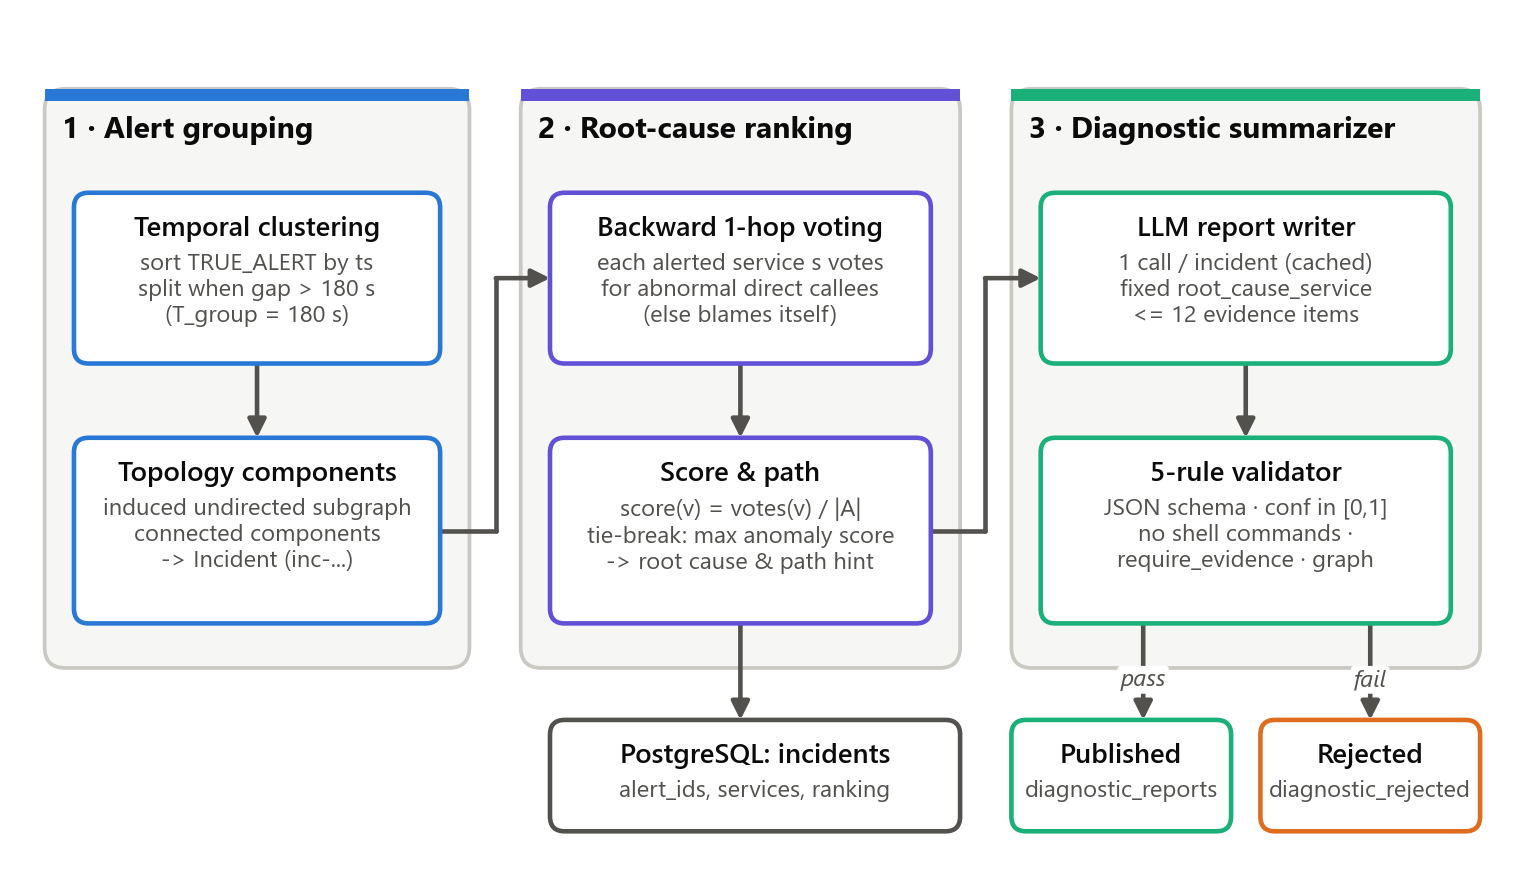
\includegraphics[width=\linewidth]{Images/C1/figures/ch4/h4.10-rca-agent.png}
  \vspace{0.35cm}
  \caption[Quy trình ba bước của tác tử RCA]{Quy trình ba bước của tác tử \term{RCA}{RCA}: gom cảnh báo ($T_{\text{group}} = 180\,\text{s}$), lan truyền ngược 1~hop và sinh báo cáo JSON qua bộ kiểm duyệt năm quy tắc. \emph{(Nguồn: tác giả vẽ, có hỗ trợ AI.)}}
  \label{fig:ch4-rca}
\end{figure}

\subsubsection{Gom cảnh báo thành sự cố}
\label{sec:ch4-grouping}

\textbf{Vấn đề giải quyết.} Một lỗi tiêm đơn lẻ thường kích hoạt nhiều cảnh báo liên tiếp trên cùng một service hoặc trên các service gọi nhau trong vài phút. Đưa từng cảnh báo rời rạc sang bước định vị gốc vừa gây trùng lặp chẩn đoán vừa làm tăng tải nhận thức cho kỹ sư vận hành.

\textbf{Thiết kế.} Thuật toán gom nhóm sự cố chạy hoàn toàn không dùng LLM theo hai bước:
\begin{enumerate}
  \item \emph{Phân cụm thời gian liên kết đơn:} Sắp xếp các cảnh báo \code{TRUE\_ALERT} tăng dần theo cặp $(t_a, \code{alert\_id})$ và tách cụm mới mỗi khi khoảng cách giữa hai cảnh báo kề nhau vượt quá ngưỡng $T_{\text{group}}$.
  \item \emph{Tách thành phần liên thông theo topology:} Trong mỗi cụm thời gian, trích đồ thị con vô hướng của đồ thị phụ thuộc $G$ cảm sinh bởi tập service có cảnh báo trong cụm (cạnh gọi theo bất kỳ chiều nào đều liên kết hai service). Mỗi thành phần liên thông tạo thành một đối tượng \code{Incident} với mã định danh tất định \code{inc-<sha256[:16]>} tính từ \code{run\_id} và danh sách \code{alert\_ids}, lưu kèm lý do gom (\code{temporal\_window\_sec} và danh sách cạnh đồ thị đã dùng). Các cảnh báo của cùng một service trong cùng cụm thời gian luôn gộp chung một sự cố.
\end{enumerate}

\textbf{Tham số, cách chọn và dẫn chiếu.} Trên tập \splitname{val}, hệ thống quét ba mức $T_{\text{group}} \in \{180, 300, 600\}\,\text{s}$ theo quy tắc lựa chọn định trước (tối thiểu số sự cố đa lỗi nhập nhằng \code{ambiguous} rồi đến \term{ARR}{ARR}). Mức $T_{\text{group}} = 180\,\text{s}$ được chốt trong cấu hình cuối của tác tử \term{RCA}{RCA} vì chỉ tạo $1$ sự cố nhập nhằng so với $2$ sự cố ở $300\,\text{s}$ và $600\,\text{s}$ (trong khi chênh lệch \term{ARR}{ARR} trên cảnh báo trong lỗi giữa $300\,\text{s}$ và $180\,\text{s}$ có CI chứa $0$). Bước gom nhóm đang dùng trong pipeline cuối và được đo bằng chỉ số \term{ARR}{ARR} ở Mục~\ref{sec:ch5-rca}.

\subsubsection{Lan truyền ngược và xếp hạng service gốc}
\label{sec:ch4-propagation}

\textbf{Vấn đề giải quyết.} Khi một sự cố gồm nhiều service có cảnh báo liên thông nhau, service chịu ảnh hưởng ở tầng trước (như cổng giao tiếp hoặc dịch vụ tổng hợp) thường có điểm bất thường cao dù lỗi gốc nằm ở dịch vụ phía sau mà nó gọi tới. Cần một thuật toán xếp hạng service gốc tận dụng chiều gọi trong đồ thị phụ thuộc để vượt qua cách xếp hạng chỉ theo điểm bất thường cực đại.

\textbf{Thiết kế.} Do phạm vi nghiên cứu ưu tiên kiểm chứng rõ ràng phương pháp tất định, đề tài hiện thực mức 1 (lan truyền ngược 1~hop \code{backward\_one\_hop}) và chủ động cắt nhánh mức 2 (dùng LLM suy luận toàn chuỗi gọi). Thuật toán khai thác quy luật lỗi lan ngược chiều gọi: khi cạnh có hướng $a \to b \in E$ tồn tại và $b$ gặp sự cố, $a$ sẽ chậm hoặc báo lỗi theo. Gọi $A$ là tập các service có cảnh báo trong sự cố và $U \supseteq A$ là tập các service có dấu hiệu bất thường trong khoảng thời gian sự cố (với cấu hình dấu hiệu \code{sign = alert} thì $U = A$; biến thể \code{sign = candidate} mở rộng thêm các service có ứng viên detector). Mỗi service $s \in A$ xác định tập đích gọi trực tiếp bất thường $\mathcal{N}^+(s) \cap U$: nếu tập này khác rỗng, $s$ chia đều $1$ phiếu bầu cho từng service trong tập đó; nếu rỗng, $s$ tự bầu $1$ phiếu cho chính mình. Điểm nghi vấn gốc của mỗi service $v$ là:
\begin{equation}
  \text{score}_{\text{RCA}}(v) = \frac{1}{|A|} \sum_{s \in A} \frac{\mathbb{I}[v \in T(s)]}{|T(s)|},
  \qquad
  T(s) =
  \begin{cases}
    \mathcal{N}^+(s) \cap U & \text{nếu } \mathcal{N}^+(s) \cap U \neq \emptyset, \\
    \{s\} & \text{ngược lại.}
  \end{cases}
  \label{eq:ch4-rca-vote}
\end{equation}
Tính phiếu theo \emph{mỗi service có cảnh báo} thay vì theo từng cảnh báo giúp thứ hạng không bị lệch nếu một service phát nhiều cảnh báo hơn các service khác. Danh sách kết quả được sắp giảm dần theo $\text{score}_{\text{RCA}}(v)$, phá hòa theo điểm bất thường cực đại của service trong khoảng sự cố rồi đến thứ tự tên service; các service trong $A$ chưa nhận phiếu vẫn được nối vào cuối danh sách để phép đo $\text{Hit}@3$ có thể đánh giá đầy đủ. Từ nút hạng 1, hàm \code{propagation\_path} dựng đường lan truyền gợi ý đi từ service gốc ra các service gọi đã bầu cho nó.

\textbf{Tham số, cách chọn và dẫn chiếu.} Trên tập \splitname{val}, mở rộng dấu hiệu bất thường sang \code{sign = candidate} chỉ tăng $+0{,}091$ $\text{Hit}@1$ với CI chạm $0$, nên cấu hình chốt giữ \code{sign = alert}. Thuật toán đang dùng trong pipeline cuối và được kiểm định đối chứng với baseline \code{rank\_by\_anomaly\_score} (xếp hạng theo điểm bất thường cao nhất trong sự cố) theo giả thuyết \hyp{H5} tại Mục~\ref{sec:ch5-rca}.

\subsubsection{Báo cáo chẩn đoán có cấu trúc JSON}
\label{sec:ch4-report}

\textbf{Vấn đề giải quyết.} Một danh sách xếp hạng tên service đơn thuần chưa đủ giúp kỹ sư trực nắm bắt loại sự cố, bằng chứng hậu thuẫn và hướng kiểm tra tiếp theo; tuy nhiên, để LLM tự do viết văn bản chẩn đoán dễ dẫn đến bịa định danh bằng chứng hoặc sinh lệnh can thiệp hệ thống nguy hiểm.

\textbf{Thiết kế và bộ kiểm duyệt.} Bộ tóm tắt chẩn đoán gọi đúng một lần API \code{gemini-2.5-flash} cho mỗi sự cố (dùng chung lớp cache JSONL với bộ thẩm định, giới hạn tối đa $1.024$ token đầu ra, truyền tối đa $12$ sự kiện bằng chứng với mỗi đoạn trích tối đa $240$ ký tự). Thiết kế tách chặt trách nhiệm: tên \code{root\_cause\_service} do hạng 1 của bước~\eqref{eq:ch4-rca-vote} ấn định và mô hình không được phép thay đổi; LLM chỉ sinh năm trường có cấu trúc theo lược đồ ở Bảng~\ref{tab:ch4-report-schema}. Để ngăn prompt thay đổi âm thầm giữa các lượt chạy, cấu hình khóa cứng mã băm dấu vân tay \code{prompt\_fingerprint = 8c1d50e6ba757ee6}. Mọi câu trả lời JSON đi qua bộ kiểm duyệt năm bước tuần tự trước khi xuất bản vào bảng \code{diagnostic\_reports}; nếu vi phạm bất kỳ quy tắc từ chối nào, bản ghi được ghi sang bảng \code{diagnostic\_rejected} kèm lý do cụ thể thay vì bỏ qua âm thầm. Tỷ lệ JSON hợp lệ được định nghĩa là số báo cáo xuất bản chia cho tổng số lần gọi LLM.

\begin{table}[H]
  \centering
  \caption{Lược đồ đầu ra \code{DiagnosticReport} và năm quy tắc kiểm duyệt tự động.}
  \label{tab:ch4-report-schema}
  \tblfont
  \tblsetup
  \begin{tabularx}{\linewidth}{|l|Y|Y|}
    \hline
    \rowcolor{gray!15}
    \textbf{Trường / Quy tắc} & \textbf{Kiểu dữ liệu \& ràng buộc} & \textbf{Xử lý khi vi phạm} \\
    \hline
    \code{fault\_type} & Một trong \code{network\_delay}, \code{cpu\_contention}, \code{exception}, \code{unknown} & Từ chối (\code{invalid\_json}) nếu ngoài danh mục \\
    \hline
    \code{confidence} & Số thực trong đoạn $[0, 1]$ & Từ chối (\code{confidence\_out\_of\_range}) \\
    \hline
    \code{evidence} & Danh sách 1--4 mã \code{event\_id} thuộc \code{allowed\_evidence\_ids} & Loại mã bịa đặt; nếu không còn mã hợp lệ $\to$ từ chối (\code{no\_evidence}) \\
    \hline
    \code{propagation\_path} & Chuỗi tên service từ gốc ra ngoài & Giữ đúng lược đồ chuỗi tên service trong prompt \\
    \hline
    \code{suggested\_actions} & 1--3 câu tiếng Anh ($\le 25$ từ) kèm mức ưu tiên \code{high}/\code{medium}/\code{low} & Chặn mọi từ lệnh (\code{kubectl}, \code{sudo}, \code{docker}, \code{rm}...) và cú pháp shell (\code{\&\&}, \code{||}, \code{\$(}) $\to$ từ chối (\code{executable\_action}) \\
    \hline
    Kiểm đồ thị dịch vụ & Kiểm \code{root\_cause\_service} $\in V$ & Vẫn xuất bản nhưng gắn cờ cảnh báo \code{suspicious = True} \\
    \hline
  \end{tabularx}
\end{table}

\textbf{Vai trò hiện tại và dẫn chiếu.} Bộ tóm tắt và kiểm duyệt JSON đang dùng trong toàn bộ luồng \term{RCA}{RCA} và dashboard sự cố; tỷ lệ JSON hợp lệ được báo cáo ở Mục~\ref{sec:ch5-rca} và chất lượng nội dung báo cáo được phân tích ở Chương~\ref{ch:thao-luan}.

% -----------------------------------------------------------------------------
\subsection{Hiện thực hóa hệ thống và harness thực nghiệm}
\label{sec:ch4-impl}

Các công nghệ thành phần đã được giới thiệu lý do lựa chọn ở Mục~\ref{sec:ch2-cong-nghe}; mục này mô tả cách tổ chức mã nguồn, lắp ráp hạ tầng lưu trữ--giao diện và vận hành harness thực nghiệm để mọi kết quả ở Chương~\ref{ch:thuc-nghiem} và kịch bản trình diễn ở Chương~\ref{ch:platform} đều tái lập được.

\textbf{Tổ chức kiến trúc mô-đun và lưu trữ hai nhánh.} Hệ thống được phân tách thành ba tầng rõ ràng: (i)~tầng thư viện lõi chứa mô hình dữ liệu Pydantic, bốn giao diện lõi, đồ thị \code{ServiceGraph} và lớp lưu trữ; (ii)~tầng dịch vụ chứa chuỗi xử lý luồng (phát lại dữ liệu, phát hiện bất thường, truy xuất ngữ cảnh, thẩm định LLM, tác tử \term{RCA}{RCA}), máy chủ API FastAPI chỉ đọc gồm tám endpoint và ứng dụng web React + TypeScript năm màn hình; (iii)~tầng thực nghiệm chứa cấu hình YAML, harness chạy thử nghiệm và kho kết quả bất biến. Toàn bộ hạ tầng đóng gói trong bốn container Docker Compose (\code{clickhouse}, \code{postgres}, \code{api}, \code{web}) hỗ trợ chạy ngoại tuyến từ cache (\code{DEMO\_OFFLINE=1}). Pipeline hợp nhất ghi đồng thời sang ClickHouse (bảng sự kiện \code{fact\_alert\_evaluation}, \code{fact\_retrieval\_trace}) và PostgreSQL (bảng quan hệ \code{run\_registry}, \code{incidents}, \code{diagnostic\_reports}, \code{diagnostic\_rejected}), kèm kiểm tra tự động \code{check\_parity} khớp $100\%$ với kết quả harness.

\textbf{Harness điều khiển bằng cấu hình và kỷ luật tái lập.} Toàn bộ thực nghiệm đều được điều khiển tập trung từ tệp cấu hình YAML thay vì gán cứng tham số trong mã nguồn; mỗi lượt chạy gắn \code{run\_id} bất biến và xuất đầy đủ tệp chứng cứ tái lập (chi tiết các lệnh vận hành và bộ kiểm thử tự động liệt kê tại Bảng~\ref{tab:ch4-harness}, Phụ lục~\ref{app:config}). Trước khi mở cổng kiểm định một lần duy nhất trên \splitname{test} (G-test), pipeline bắt buộc vượt qua hai cổng kỹ thuật G-port (Mục~\ref{sec:ch5-gport}) và G-paper (Mục~\ref{sec:ch5-gpaper}).

% -----------------------------------------------------------------------------
\subsection{Kết chương}
\label{sec:ch4-ket-chuong}

Chương này đã trình bày hoàn chỉnh thiết kế và hiện thực hóa của nền tảng AIOps gồm bốn khâu từ phát hiện bất thường đến trực quan hóa sự cố. Trong nhánh thẩm định cảnh báo, cấu hình \CTAV{} chốt sau quá trình kiểm chứng tách biệt trên tập \splitname{val} gồm bộ phát hiện Isolation Forest (ngưỡng $0{,}85$), truy xuất lai \term{BM25}{BM25}--topology \textbf{\comp{C1}} ($\alpha = 0{,}35$, $\beta = 0{,}25$, $\gamma = 0{,}40$, $\tau_F = 300\,\text{s}$, bán kính 2 hop), bộ thẩm định \code{gemini-2.5-flash} qua cache bất biến, ngưỡng tin cậy $\theta_{\text{local}} = 0{,}80$ và quy tắc neo bằng chứng bất thường \textbf{\comp{C3}} dựa trên ngưỡng nền \splitname{dev} $p_{90}$. Ba cơ chế khác trong không gian thiết kế đã được ghi nhận rõ vai trò thực tế: ngưỡng bất đối xứng \textbf{\comp{C2}} và định tuyến hai tầng \textbf{\comp{C4}} đã bị loại sau kiểm định loại trừ trên \splitname{val}, còn cổng cứu cảnh báo \textbf{\comp{C5}} (\code{Rescue Score}) chỉ giữ làm phân tích loại trừ độc lập. Ở nhánh phân tích nguyên nhân gốc, tác tử \term{RCA}{RCA} ghép nối ba bước gồm gom cảnh báo theo thời gian ($T_{\text{group}} = 180\,\text{s}$) và thành phần liên thông đồ thị, bỏ phiếu lan truyền ngược 1 bước theo chiều gọi (\code{sign = alert}), và sinh báo cáo JSON có kiểm duyệt năm quy tắc qua cùng lớp cache. Toàn bộ phương pháp đã được đóng gói vào harness điều khiển bằng cấu hình YAML cùng bộ lưu trữ ClickHouse/PostgreSQL để sẵn sàng cho bước kiểm định định lượng các giả thuyết \hyp{H0}--\hyp{H5} trong Chương~\ref{ch:thuc-nghiem}.

 \newpage
 % =============================================================================
% Chuong 5: Thuc nghiem va danh gia (chuan lop article cho Internship2_HK262)
% =============================================================================

\section{Thực nghiệm và đánh giá}
\label{ch:thuc-nghiem}

Chương này kiểm chứng toàn diện đề xuất \CTAV{} và tác tử RCA theo trình tự thực nghiệm ba lớp: kiểm tra tính đúng của pipeline cơ sở và khả năng tái lập hồi quy (Mục~\ref{sec:ch5-gates}), tinh chỉnh và chọn cấu hình trên tập \splitname{val} (Mục~\ref{sec:ch5-val}), cuối cùng kiểm định một lần duy nhất trên tập \splitname{test} đã niêm phong cho cả nhánh thẩm định cảnh báo lẫn nhánh phân tích nguyên nhân gốc (Mục~\ref{sec:ch5-test}--\ref{sec:ch5-rca}). Mở đầu chương, các mục từ~\ref{sec:ch5-hypotheses} đến~\ref{sec:ch5-metrics} trình bày sáu giả thuyết đăng ký trước H0--H5, giao thức chia dữ liệu chống rò rỉ, thiết lập thực nghiệm và hệ thống thước đo. Mục~\ref{sec:ch5-synthesis} tổng hợp mười hai phát hiện thực nghiệm định hình các quyết định thiết kế, và Mục~\ref{sec:ch5-ket-chuong} tóm tắt kết luận kiểm định trước khi chuyển sang phần trình diễn nền tảng ở Chương~\ref{ch:platform}.

% -----------------------------------------------------------------------------
\subsection{Mục tiêu thực nghiệm và các giả thuyết H0--H5}
\label{sec:ch5-hypotheses}

Thực nghiệm của đề tài hướng tới hai mục tiêu định lượng đã xác lập ở Chương~\ref{ch:mo-dau}: (A) kiểm chứng liệu \CTAV{} có duy trì mức tăng thu hồi (recall) của truy xuất nhận biết topology mà không làm tăng tỷ lệ báo động giả (FPR) so với truy xuất từ khóa cục bộ BM25 trong cùng ngân sách gọi LLM hay không; và (B) kiểm chứng liệu tác tử RCA đứng sau \CTAV{} có định vị được service gốc, giảm số cảnh báo qua gom sự cố và sinh báo cáo chẩn đoán hợp lệ hay không.

Để ngăn ngừa tinh chỉnh hậu nghiệm, toàn bộ sáu giả thuyết H0--H5 cùng tiêu chí chấp nhận và cấu hình đóng băng đã được đăng ký công khai trong kho mã nguồn tại một commit riêng (\code{be2b985}) trước bất kỳ lượt chạy nào trên tập \splitname{test}. Quy ước thống kê áp dụng đồng nhất gồm: khoảng tin cậy 95\% (CI95) ước lượng bằng bootstrap phân vị 1.000 mẫu (\code{seed = 42}) và kiểm định McNemar chính xác hai phía ở mức ý nghĩa $\alpha = 0{,}05$. Trong đó, \textbf{H2} là giả thuyết chính; các giả thuyết H0, H3, H4 là giả thuyết phụ, báo giá trị $p$ thô không hiệu chỉnh đa so sánh. Chỉ số chính của nhánh thẩm định tính trên tập con \emph{cửa sổ có telemetry}; kết quả trên toàn bộ split được báo làm chỉ số phụ. Bảng~\ref{tab:h0-h5} liệt kê nguyên văn tiêu chí chấp nhận đã đăng ký cho H0--H5.

\begin{table}[htbp]
  \centering
  \caption[Giả thuyết H0--H5 và tiêu chí chấp nhận đã đăng ký]{Hệ thống giả thuyết H0--H5 và tiêu chí chấp nhận đã đăng ký trước khi chạm tập \splitname{test}.}
  \label{tab:h0-h5}
  \scriptsize
  \renewcommand{\arraystretch}{1.15}
  \setlength{\tabcolsep}{3.5pt}
  \begin{tabularx}{\linewidth}{@{}l >{\raggedright\arraybackslash}p{3.6cm} Y >{\raggedright\arraybackslash}p{2.3cm}@{}}
    \toprule
    \textbf{Mã} & \textbf{Nội dung giả thuyết} & \textbf{Tiêu chí chấp nhận đã đăng ký (\code{be2b985})} & \textbf{Phạm vi kiểm} \\
    \midrule
    \textbf{H0} & Topology chưa hiệu chỉnh (C1) tăng recall và tăng FPR so với BM25 & CI95 của $\Delta\text{Recall}$ và $\Delta\text{FPR}$ có cận dưới $> 0$; McNemar trên cửa sổ lỗi và bình thường đều $p < 0{,}05$ & \splitname{val} \& \splitname{test} \\
    \textbf{H1} & Cơ chế: \code{TRUE\_ALERT} trên cửa sổ bình thường tăng theo độ gần thời gian và loại bằng chứng (trace) & Xu hướng đơn điệu dương kèm CI95 trên mẫu can thiệp cố định; không chạy lại trên \splitname{test} & Chỉ \splitname{val} \\
    \textbf{H2} (chính) & \CTAV{} tốt hơn BM25 và giữ phần lớn recall của C1 & (i)~CI95 $\Delta\text{F1}(\text{\CTAV}-\text{BM25})$ cận dưới $> 0$ và McNemar $p < 0{,}05$; (ii)~CI95 $\Delta\text{FPR}(\text{\CTAV}-\text{BM25})$ không có cận dưới $> 0$; (iii)~ước lượng điểm $\Delta\text{Recall}(\text{\CTAV}-\text{C1}) \ge -0{,}05$. Đạt (i)--(ii) nhưng trượt (iii) $\Rightarrow$ ``đạt một phần'' & \splitname{val} (sơ bộ) \& \splitname{test} \\
    \textbf{H3} & Đóng góp từng thành phần quanh \CTAV{} (một-thay-đổi-một-lần) & Bỏ C3 $\Rightarrow$ CI95 $\Delta\text{Precision}$ cận trên $< 0$; thêm C2 xác nhận loại nếu CI95 $\Delta\text{FPR}$ chứa $0$ hoặc $> 0$; thêm C4 xác nhận loại nếu chi phí tăng và CI95 $\Delta\text{F1}$ không có cận dưới $> 0$; báo mô tả C3-trượt và C5 một điểm & \splitname{val} \& \splitname{test} \\
    \textbf{H4} & Ở ngân sách 120 lần gọi, \CTAV{} không kém LLM-không-RAG & Ước lượng điểm $\text{F1}(\text{\CTAV}) \ge \text{F1}(\text{không-RAG})$ ở mốc 120 lần gọi; báo kèm toàn bộ đường ngân sách & \splitname{val} \& \splitname{test} \\
    \textbf{H5} & Tác tử RCA định vị service gốc và giảm cảnh báo & $\text{Hit@1} \ge 0{,}60$, $\text{Hit@3} \ge 0{,}80$, cận dưới CI95 của $\Delta\text{Hit@1}(\text{RCA}-\text{baseline}) > 0$, và Alert Reduction $\ge 30\%$ trên sự cố cascade & \splitname{val} \& \splitname{test} \\
    \bottomrule
  \end{tabularx}
\end{table}

% -----------------------------------------------------------------------------
\subsection{Dữ liệu và giao thức chia split chống rò rỉ}
\label{sec:ch5-data}

Toàn bộ thí nghiệm sử dụng bộ dữ liệu microservice đa phương thức công khai Nezha~\cite{nezha} (gồm hai hệ thống OnlineBoutique và TrainTicket với năm loại lỗi tiêm có chủ đích: \code{network\_delay}, \code{cpu\_contention}, \code{cpu\_consumed}, \code{exception}, \code{return}). Đồ thị phụ thuộc service dựng từ cặp \code{SpanID}--\code{ParentID} của trace gồm $56$ service và $68$ cạnh có hướng. Dữ liệu được cắt thành các cửa sổ không chồng lấn độ dài $60\,\text{s}$ và gán nhãn theo thời gian thực (\emph{wall-clock}) như trình bày ở Mục~\ref{sec:ch2-du-lieu}.

Để loại bỏ rò rỉ dữ liệu theo thời gian và theo cùng một sự cố, đề tài áp dụng giao thức chia ba tập \splitname{dev}, \splitname{val}, \splitname{test} cố định bằng \code{seed = 42}, minh họa ở Hình~\ref{fig:ch5-split}. Toàn bộ $7$ cửa sổ của mỗi lần tiêm lỗi (\code{injection\_id}) luôn nằm trọn trong cùng một split; $597$ cửa sổ bình thường của cùng pod nằm trong vùng đệm $600\,\text{s}$ quanh thời điểm tiêm lỗi bị loại bỏ để tránh dính dư chấn lỗi; các cửa sổ bình thường còn lại được phân bổ nguyên khối theo cặp \code{ngày|pod} và \emph{không lấy mẫu giảm bớt} (giữ nguyên tỷ lệ mất cân bằng tự nhiên xấp xỉ $1:135$). Trong đó, \splitname{dev} chỉ dùng để huấn luyện bộ phát hiện, dựng ngưỡng nền C3 và gỡ lỗi; \splitname{val} dùng để chạy H1 và chọn cấu hình; \splitname{test} bị niêm phong và chỉ chạy một lần sau khi đăng ký giả thuyết.

\begin{figure}[htbp]
  \centering
  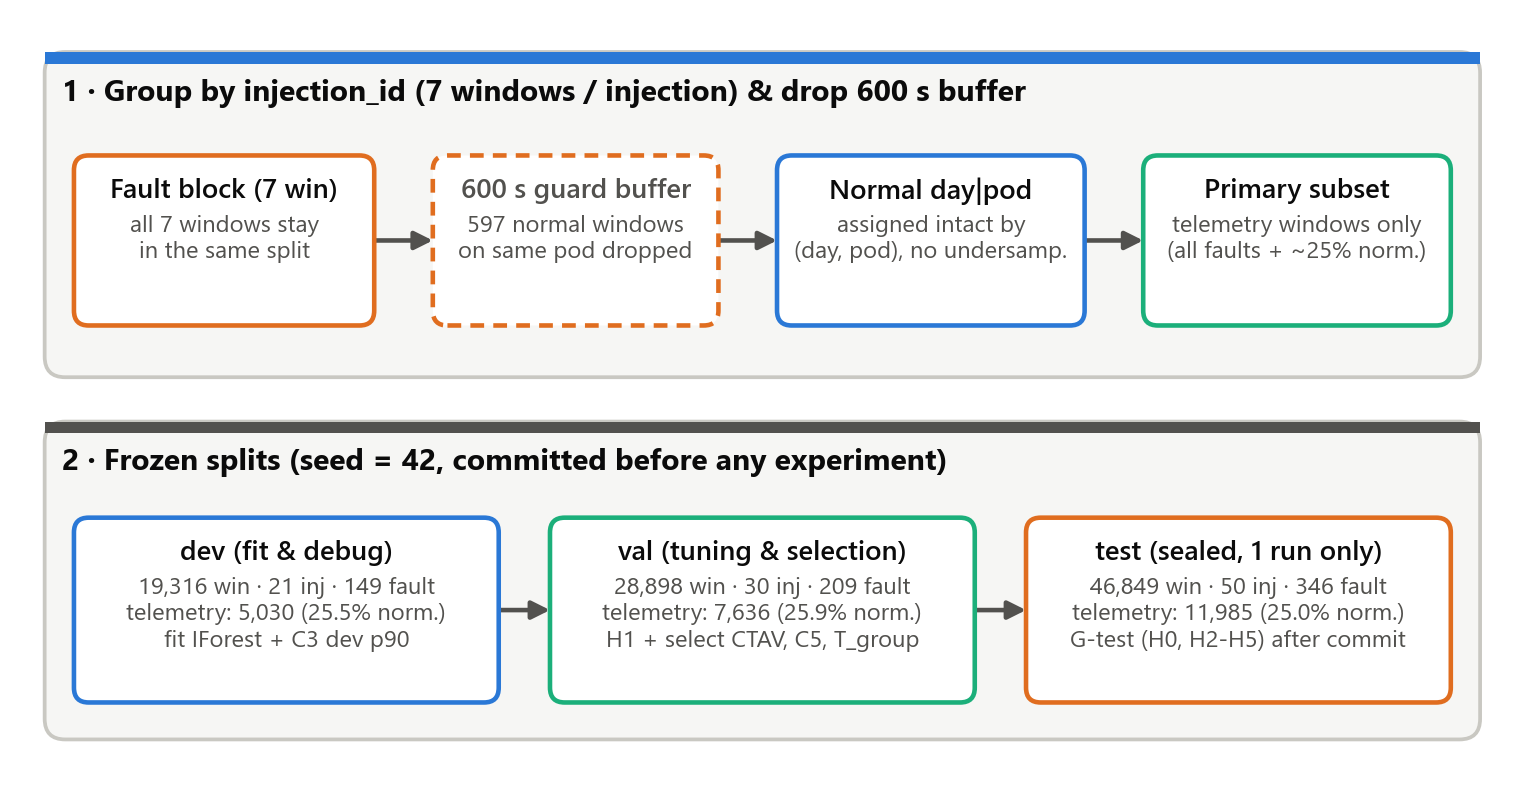
\includegraphics[width=\linewidth]{Images/C1/figures/ch5/h5.1-split-protocol.png}
  \vspace{0.35cm}
  \caption[Giao thức chia dữ liệu chống rò rỉ theo lần tiêm lỗi]{Giao thức chia split chống rò rỉ trên Nezha: giữ nguyên khối 7 cửa sổ mỗi lần tiêm lỗi, loại vùng đệm 600~s và khóa cứng ba tập \splitname{dev}, \splitname{val}, \splitname{test}. \emph{(Nguồn: tác giả vẽ, có hỗ trợ AI.)}}
  \label{fig:ch5-split}
\end{figure}

Bảng~\ref{tab:ch5-splits} thống kê kích thước ba split, đồng thời chỉ ra một đặc điểm cấu trúc quan trọng của Nezha (\textbf{Phát hiện 1}): bộ dữ liệu chỉ lưu tệp log và trace xung quanh các khoảng thời gian tiêm lỗi. Mọi cửa sổ lỗi ($100\%$) đều có dữ liệu log hoặc trace, trong khi chỉ khoảng $25\%$ cửa sổ bình thường có telemetry kèm theo. Trên tập đối chiếu mẫu nhỏ của nghiên cứu tiền đề~\cite{icaetm2026}, khảo sát độ phủ ở Bảng~\ref{tab:ch5-coverage} cho thấy chỉ $5{,}4\%$ cửa sổ bình thường truy xuất được bằng chứng khác rỗng trong kho đã lọc theo nhãn ($19{,}4\%$ trong kho đầy đủ), đồng nghĩa sự hiện diện của bằng chứng gần như trùng khớp với dấu hiệu gần sự cố. Để tránh việc bộ thẩm định thắng giả nhờ từ chối các cửa sổ thiếu dữ liệu, tập chấm chính của đề tài được giới hạn trên các \emph{cửa sổ có telemetry} ($5.030$ cửa sổ trên \splitname{dev}, $7.636$ trên \splitname{val} và $11.985$ trên \splitname{test}).

\begin{table}[htbp]
  \centering
  \caption[Kích thước các split và tỷ lệ cửa sổ có telemetry trên Nezha]{Kích thước ba split \splitname{dev}, \splitname{val}, \splitname{test} và tỷ lệ cửa sổ có dữ liệu telemetry đi kèm.}
  \label{tab:ch5-splits}
  \scriptsize
  \renewcommand{\arraystretch}{1.15}
  \begin{tabularx}{\linewidth}{@{}l r r r r Y@{}}
    \toprule
    \textbf{Split} & \textbf{Tổng cửa sổ} & \textbf{Cửa sổ lỗi} & \textbf{Lần tiêm lỗi} & \textbf{Lỗi có telemetry} & \textbf{Bình thường có telemetry} \\
    \midrule
    \splitname{dev} & 19.316 & 149 & 21 & 149 / 149 (100\%) & 4.881 / 19.167 (25,5\%) \\
    \splitname{val} & 28.898 & 209 & 30 & 209 / 209 (100\%) & 7.427 / 28.689 (25,9\%) \\
    \splitname{test} & 46.849 & 346 & 50 & 346 / 346 (100\%) & 11.639 / 46.503 (25,0\%) \\
    \bottomrule
  \end{tabularx}
\end{table}

\begin{table}[htbp]
  \centering
  \caption[Độ phủ bằng chứng giữa cửa sổ lỗi và cửa sổ bình thường]{Độ phủ bằng chứng trên tập mẫu đối chiếu ($98$ cửa sổ lỗi, $391$ cửa sổ bình thường), làm rõ động lực chọn tập chấm chính trên cửa sổ có telemetry.}
  \label{tab:ch5-coverage}
  \scriptsize
  \renewcommand{\arraystretch}{1.15}
  \begin{tabularx}{\linewidth}{@{}Y r r@{}}
    \toprule
    \textbf{Điều kiện tồn tại bằng chứng} & \textbf{Cửa sổ lỗi (98)} & \textbf{Cửa sổ bình thường (391)} \\
    \midrule
    Kho đối chiếu lọc theo nhãn: top-6 khác rỗng & 89 (90,8\%) & 21 (5,4\%) \\
    Kho Nezha đầy đủ: top-6 khác rỗng & 98 (100,0\%) & 76 (19,4\%) \\
    Có tệp log hoặc trace trong biên $\pm 8$ phút & 98 (100,0\%) & 106 (27,1\%) \\
    \bottomrule
  \end{tabularx}
\end{table}

% -----------------------------------------------------------------------------
\subsection{Thiết lập thực nghiệm và chi phí}
\label{sec:ch5-setup}

Mọi thí nghiệm thẩm định chính thức sử dụng một mô hình API duy nhất là \code{gemini-2.5-flash} ở nhiệt độ $0$, tắt vùng suy luận ẩn (\code{thinkingBudget = 0}), bỏ cột metric hằng lỗi \code{PodSuccessRate(\%)} khỏi prompt (\textbf{Phát hiện 5}), và đi qua lớp cache JSONL khóa \code{sha256} (Mục~\ref{sec:ch4-judge}). Riêng cổng kiểm chứng hồi quy G-paper đọc lại trực tiếp tệp cache của mô hình \code{gemini-2.5-flash-lite} với tỷ lệ trúng cache $100\%$. Bộ phát hiện Isolation Forest (ngưỡng $0{,}85$, \code{buffer\_size = 2}) được huấn luyện duy nhất trên \splitname{dev}. Truy xuất C1 sử dụng cấu hình $\alpha = 0{,}35$, $\beta = 0{,}25$, $\gamma = 0{,}40$, $\tau_F = 300\,\text{s}$, mở rộng $2$ hop, top-$6$ trong $4.000$ token với engine vector hóa (trung bình $\approx 0{,}45\,\text{s}$ mỗi truy vấn).

Các lượt gọi API chạy song song 8 luồng với bộ giới hạn tốc độ 200 lượt gọi/phút; toàn bộ đánh giá \CTAV{} và các nhánh loại trừ H3 được thực hiện bằng chế độ phát lại trên phán quyết đã lưu cache (\code{py -m eval ctav}, chi phí $0$ USD). Bảng~\ref{tab:ch5-costs} tổng hợp chi phí ước tính theo đơn giá token của toàn bộ chiến dịch thực nghiệm; lưu ý đây là chi phí quy đổi từ số lượng token ghi trong sổ cái cache, chưa đối chiếu trực tiếp với hóa đơn thanh toán cuối cùng của nhà cung cấp.

\begin{table}[htbp]
  \centering
  \caption[Tổng hợp chi phí gọi API LLM theo các hạng mục thực nghiệm]{Chi phí gọi API LLM ước tính theo sổ cái token cho từng hạng mục thực nghiệm chính.}
  \label{tab:ch5-costs}
  \scriptsize
  \renewcommand{\arraystretch}{1.15}
  \begin{tabularx}{\linewidth}{@{}l Y r Y@{}}
    \toprule
    \textbf{Hạng mục} & \textbf{Nội dung chạy chính} & \textbf{USD theo token} & \textbf{Ghi chú} \\
    \midrule
    Kiểm chứng G-port / G-paper & Khớp pipeline mock + tái lập 489 ca từ cache + smoke test & 0,29 & G-paper đạt 100\% cache hit (0 USD) \\
    Thực nghiệm H0 trên \splitname{val} & BM25, C1 ($k_{\text{graph}} \in \{0, 1\}$), LLM-không-RAG & $\approx 8{,}60$ & Có phần tái sử dụng cache giữa các nhánh \\
    Thí nghiệm cơ chế H1 trên \splitname{val} & 9 điều kiện can thiệp (6.988 lượt gọi thành công) & 9,48 & Dùng mẫu cố định 1.749 candidate \\
    Chọn cấu hình \CTAV{} & Replay toàn bộ chính sách và ablation H3 trên \splitname{val} & 0,00 & Mô phỏng C1 mọi candidate $\approx 3{,}28$ USD/run \\
    Khảo sát C5 trên \splitname{val} & Chấm một lần 1.459 cửa sổ được cứu & 1,03 & Quét 147 điểm lưới ngoại tuyến \\
    Kiểm định G-test trên \splitname{test} & BM25, C1, không-RAG, C5 một điểm, 4 run \code{repeat} & 15,85 & 21.094 lượt gọi API mới, 0 lỗi judge \\
    Tác tử RCA (\splitname{val} \& \splitname{test}) & Tóm tắt 26 (\splitname{val}) + 38 (\splitname{test}) + 114 (độ nhạy) sự cố & 0,28 & Tổng 178 lượt gọi, 0 báo cáo bị loại \\
    \bottomrule
  \end{tabularx}
\end{table}

% -----------------------------------------------------------------------------
\subsection{Thước đo đánh giá}
\label{sec:ch5-metrics}

Các công thức định nghĩa thước đo đã được trình bày ở Mục~\ref{sec:ch2-danh-gia}; mục này chốt quy ước áp dụng thống nhất cho toàn chương:
\begin{itemize}
  \item \emph{Nhánh thẩm định cảnh báo:} Báo cáo \code{TP}, \code{FP}, Precision, Recall, F1 (lấy 3 chữ số thập phân) và FPR (lấy 4 chữ số thập phân do FPR của \CTAV{} ở hàng phần nghìn). Recall luôn tính trên \emph{tổng số cửa sổ lỗi của split} (kể cả cửa sổ bị bộ phát hiện bỏ sót); trạng thái \code{UNCERTAIN} và \code{manual\_review} không tính là cảnh báo phát ra.
  \item \emph{Kiểm định thống kê và độ ổn định:} Mọi hiệu ghép cặp $\Delta = \text{phương pháp} - \text{đối chứng}$ kèm CI95 bootstrap 1.000 mẫu (\code{seed = 42}) và giá trị $p$ của kiểm định McNemar chính xác tách riêng trên cửa sổ lỗi và cửa sổ bình thường. Độ ổn định của judge được đo bằng tỷ lệ lật phán quyết qua ba lần gọi độc lập \code{repeat} $\in \{0, 1, 2\}$ trên tập con 200 candidate.
  \item \emph{Nhánh phân tích nguyên nhân gốc:} Đánh giá $\text{Hit@1}$, $\text{Hit@3}$ trên các sự cố có nhãn đơn lỗi (loại sự cố đa lỗi nhập nhằng \code{ambiguous} và báo rõ số lượng), đối chiếu với baseline xếp hạng theo điểm bất thường cao nhất; đo \emph{Alert Reduction Ratio} ($\text{ARR} = 1 - \text{\#sự cố}/\text{\#cảnh báo}$), tỷ lệ JSON hợp lệ (\emph{JSON valid rate}) và độ trễ hồi phát.
\end{itemize}

% -----------------------------------------------------------------------------
\subsection{Kiểm chứng tính đúng của pipeline và tái lập hồi quy}
\label{sec:ch5-gates}

Trước khi chạy các thí nghiệm khoa học trên giao thức chống rò rỉ mới, hệ thống phải vượt qua hai cổng kiểm chứng kỹ thuật là G-port và G-paper (đặt trên cùng trục ba cổng kiểm chứng với G-test ở Hình~\ref{fig:ch5-gates}).

\begin{figure}[htbp]
  \centering
  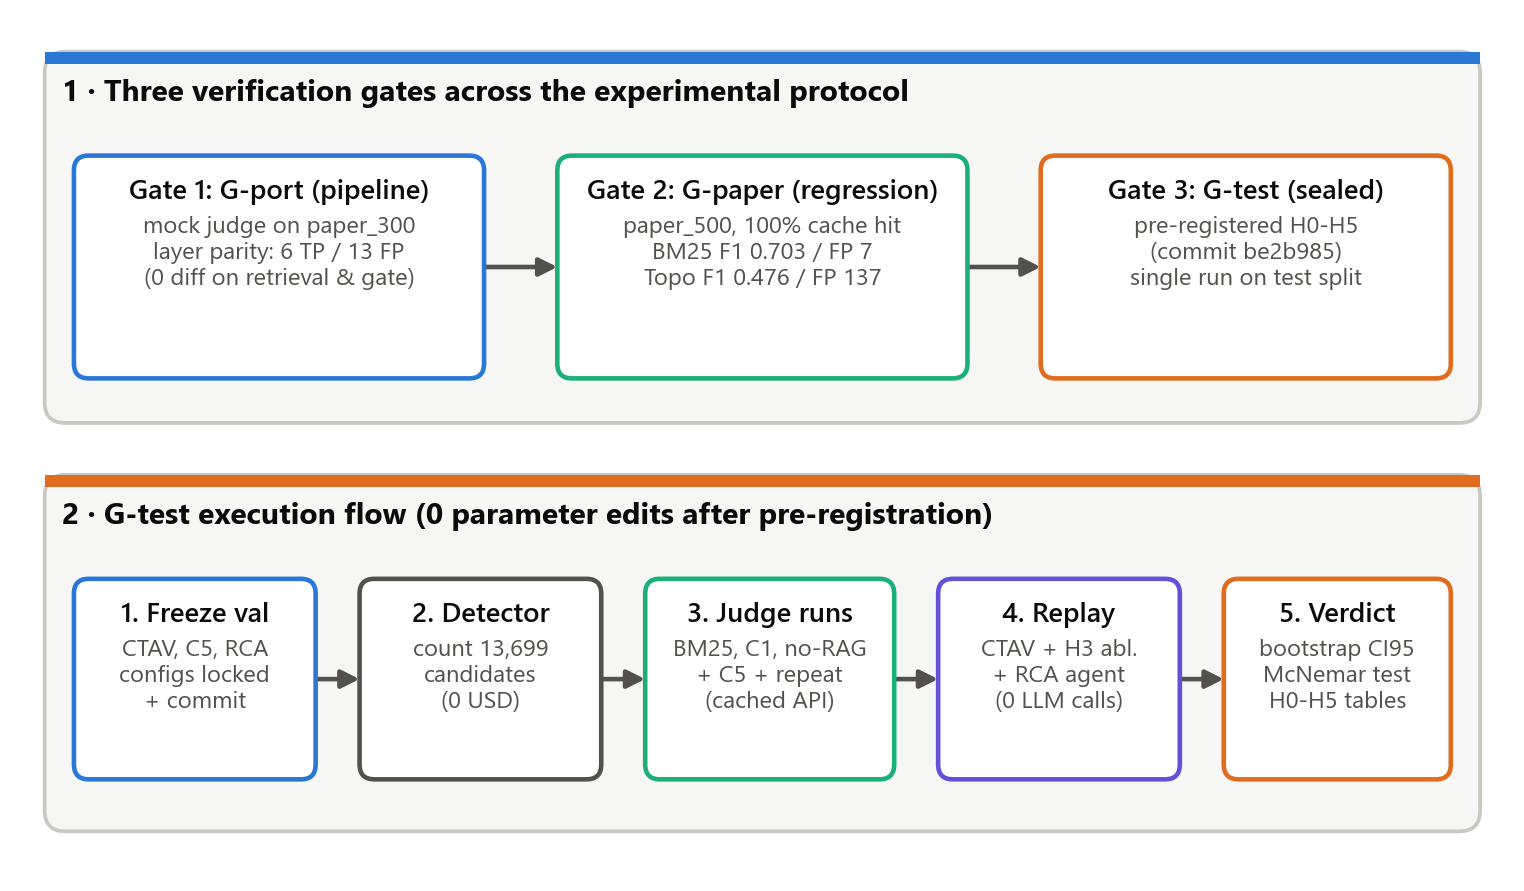
\includegraphics[width=\linewidth]{Images/C1/figures/ch5/h5.3-three-gates.png}
  \vspace{0.35cm}
  \caption[Ba cổng kiểm chứng kỹ thuật và luồng thực thi G-test]{Ba cổng kiểm chứng thực nghiệm (G-port, G-paper, G-test) và quy trình năm bước khép kín của G-test sau khi đăng ký trước giả thuyết tại commit \code{be2b985}. \emph{(Nguồn: tác giả vẽ, có hỗ trợ AI.)}}
  \label{fig:ch5-gates}
\end{figure}

\subsubsection{Kiểm chứng pipeline cơ sở (G-port)}
\label{sec:ch5-gport}

Cổng G-port đối chiếu hành vi từng tầng của pipeline hiện thực với bản tham chiếu đã chốt bằng bộ thẩm định giả lập (\emph{mock judge}) trên tập \code{paper\_300} (ngưỡng $0{,}95$, cổng tin cậy $0{,}80 / 0{,}98$, ngân sách $30$ lượt gọi; kết quả tham chiếu: Precision $0{,}3158$ với $6$ TP / $13$ FP, Recall $0{,}375$, FPR $0{,}0458$). Kết quả kiểm chứng phân rã theo từng tầng ở Bảng~\ref{tab:ch5-gport} cho thấy ba tầng lõi — truy xuất BM25 ($40/40$ top-6 trùng), bộ thẩm định giả lập ($30/30$) và tầng cổng ngân sách khi nhận cùng đầu vào ứng viên ($6$ TP / $13$ FP / $10$ FN / $271$ TN) — khớp tuyệt đối $100\%$. Khi chạy toàn pipeline với bộ phát hiện Isolation Forest mới trên cửa sổ $60\,\text{s}$, số FP lệch $+6$ ($6/19/10/265$, tương quan thứ hạng Spearman $0{,}79$) do sự khác biệt tự nhiên của đặc trưng bộ đệm cuộn; kiểm chứng cho thấy $10/13$ FP ở bản tham chiếu phát sinh từ luật ``hết ngân sách tự động đẩy cảnh báo'', không phải từ bộ thẩm định. Cổng G-port được xác nhận đạt theo tầng; các con số với bộ thẩm định giả lập chỉ phục vụ kiểm chứng phần mềm và không dùng để rút kết luận khoa học.

\begin{table}[htbp]
  \centering
  \caption[Kết quả kiểm chứng pipeline cơ sở G-port theo từng tầng]{Kiểm chứng từng tầng của cổng G-port trên tập \code{paper\_300} (dùng bộ thẩm định giả lập, chỉ kiểm chứng tính đúng kỹ thuật).}
  \label{tab:ch5-gport}
  \scriptsize
  \renewcommand{\arraystretch}{1.15}
  \begin{tabularx}{\linewidth}{@{}l Y l@{}}
    \toprule
    \textbf{Tầng kiểm chứng} & \textbf{Kết quả đo được} & \textbf{Đánh giá} \\
    \midrule
    1. Truy xuất BM25 & Top-6 trùng khớp tuyệt đối $40/40$ truy vấn & Đạt \\
    2. Bộ thẩm định giả lập (mock) & Phán quyết trùng khớp tuyệt đối $30/30$ ca & Đạt \\
    3a. Cổng ngưỡng \& ngân sách (cùng đầu vào ứng viên) & Ma trận nhầm lẫn $6/13/10/271$ trùng tuyệt đối bản tham chiếu & Đạt \\
    3b. Toàn pipeline với bộ phát hiện cửa sổ 60~s & $6/19/10/265$ (lệch $+6$ FP; Spearman điểm detector $0{,}79$) & Chấp nhận theo tầng \\
    \bottomrule
  \end{tabularx}
\end{table}

\subsubsection{Kiểm chứng hồi quy trên tập đối chiếu (G-paper)}
\label{sec:ch5-gpaper}

Cổng G-paper kiểm tra khả năng tái lập chính xác hai mốc baseline đã công bố trong khảo sát bước đầu~\cite{icaetm2026} trên tập \code{paper\_500} ($100$ cửa sổ lỗi, $400$ cửa sổ bình thường, mô hình \code{gemini-2.5-flash-lite}, ngân sách đầy đủ) hoàn toàn từ lớp cache mà không phát sinh bất kỳ lượt gọi API mới nào. Như trình bày trong Bảng~\ref{tab:ch5-gpaper}, cả hai chiến lược BM25 và Topology đều khớp $489/489$ truy vấn về top-6 bằng chứng, chuỗi prompt và khóa cache ($100\%$ cache hit), tái lập chính xác từng con số đã công bố (BM25 đạt F1 $0{,}7030$ với $7$ FP; Topology đạt F1 $0{,}4759$ với $137$ FP).

\begin{table}[htbp]
  \centering
  \caption[Kết quả kiểm chứng hồi quy G-paper trên tập đối chiếu]{Kiểm chứng hồi quy G-paper trên \code{paper\_500} (\code{gemini-2.5-flash-lite}, tỷ lệ trúng cache $100\%$, $0$ lượt gọi API mới).}
  \label{tab:ch5-gpaper}
  \scriptsize
  \renewcommand{\arraystretch}{1.15}
  \begin{tabularx}{\linewidth}{@{}l Y r r r r r@{}}
    \toprule
    \textbf{Biến thể} & \textbf{Khớp top-6 / prompt / cache} & \textbf{TP} & \textbf{FP} & \textbf{Precision} & \textbf{Recall} & \textbf{F1 (công bố)} \\
    \midrule
    BM25 & $489/489/489$ & 58 & 7 & 0,8923 & 0,580 & 0,7030 (0,7030) \\
    Topology & $489/489/489$ & 74 & 137 & 0,3507 & 0,740 & 0,4759 (0,4759) \\
    \bottomrule
  \end{tabularx}
\end{table}

Quá trình giải phẫu cổng G-paper đồng thời bộc lộ ba phát hiện nền tảng về giao thức cũ: độ tin cậy mô hình trả ra phần lớn sao chép trực tiếp từ \code{anomaly\_score} khi thiếu ngữ cảnh (\textbf{Phát hiện 2}); biến thể ``topology'' trên tập mẫu cũ thực chất hoạt động gần giống BM25 không giới hạn thời gian (\textbf{Phát hiện 3}); và khi cài đặt đúng công thức Fusion Score trên kho đầy đủ, C1 không hề đưa bằng chứng từ service lân cận vào top-6 nếu không có hạn ngạch (\textbf{Phát hiện 4}). Những phát hiện này là cơ sở trực tiếp để thiết kế thí nghiệm H0 và H1 trên tập \splitname{val} ở mục tiếp theo.

% -----------------------------------------------------------------------------
\subsection{Tinh chỉnh và lựa chọn cấu hình trên tập \splitname{val}}
\label{sec:ch5-val}

Toàn bộ các quyết định chọn tham số và tinh gọn thành phần của \CTAV{}, cổng C5 và tác tử RCA đều được thực hiện trên tập \splitname{val} ($7.636$ cửa sổ có telemetry, $209$ cửa sổ lỗi, $1.749$ candidate của bộ phát hiện) mà không đọc bất kỳ dữ liệu nào của \splitname{test}.

\subsubsection{Kiểm chứng sơ bộ H0 trên \splitname{val}}
\label{sec:ch5-val-h0}

Bảng~\ref{tab:ch5-val-h0} và Bảng~\ref{tab:ch5-val-h0-diff} trình bày kết quả đối chiếu năm phương pháp trên tập \splitname{val}. So với BM25, C1 không hạn ngạch (\code{k\_graph = 0}) tăng Recall thêm $+0{,}100$ $[+0{,}052;\, +0{,}155]$ ($55$ so với $34$ TP, McNemar $p < 0{,}001$) nhưng đồng thời đẩy FPR tăng $+0{,}0254$ $[+0{,}0204;\, +0{,}0306]$ ($606$ so với $417$ FP, $p < 0{,}001$), còn hiệu $\Delta\text{F1} = +0{,}023$ $[-0{,}004;\, +0{,}052]$ có CI95 chứa $0$. Tuy hiện tượng ``tăng cả recall lẫn FPR'' lặp lại cùng chiều với khảo sát tiền đề, phân tích chênh lệch bằng chứng cho thấy biến thể ép thêm bằng chứng lân cận (\code{C1-quota}, $k_{\text{graph}} = 1$) cho kết quả gần như đồng nhất với \code{C1-paper} ($\Delta\text{F1} = -0{,}001$, $p > 0{,}15$). Nguyên nhân thực tế là C1 chọn nhiều trace span của \emph{chính service phát cảnh báo} nằm sát trung điểm $t_0$ hơn BM25 (trung vị $|\Delta t|$ là $66$--$73\,\text{s}$ so với $139$--$167\,\text{s}$, \textbf{Phát hiện 7}).

\begin{table}[htbp]
  \centering
  \caption[So sánh các phương pháp nền trên tập val]{Kết quả các phương pháp nền trên tập \splitname{val} (cửa sổ có telemetry: $7.636$ cửa sổ, $209$ lỗi).}
  \label{tab:ch5-val-h0}
  \scriptsize
  \renewcommand{\arraystretch}{1.15}
  \setlength{\tabcolsep}{3.5pt}
  \begin{tabularx}{\linewidth}{@{}Y r r r c c r@{}}
    \toprule
    \textbf{Phương pháp} & \textbf{TP} & \textbf{FP} & \textbf{Precision} & \textbf{Recall [CI95]} & \textbf{F1 [CI95]} & \textbf{FPR} \\
    \midrule
    Detector-only & 109 & 1.640 & 0,062 & 0,522 [0,454; 0,589] & 0,111 [0,094; 0,131] & 0,2208 \\
    BM25 & 34 & 417 & 0,075 & 0,163 [0,115; 0,214] & 0,103 [0,072; 0,133] & 0,0561 \\
    C1-paper ($k_{\text{graph}} = 0$) & 55 & 606 & 0,083 & 0,263 [0,205; 0,326] & 0,126 [0,095; 0,156] & 0,0816 \\
    C1-quota ($k_{\text{graph}} = 1$) & 53 & 585 & 0,083 & 0,254 [0,197; 0,315] & 0,125 [0,094; 0,156] & 0,0788 \\
    LLM-không-RAG & 18 & 166 & 0,098 & 0,086 [0,052; 0,128] & 0,092 [0,056; 0,134] & 0,0224 \\
    \bottomrule
  \end{tabularx}
\end{table}

\begin{table}[htbp]
  \centering
  \caption[Hiệu ghép cặp và kiểm định McNemar cho H0 trên tập val]{Hiệu ghép cặp và giá trị $p$ của kiểm định McNemar trên tập \splitname{val} ($7.636$ cửa sổ có telemetry, $209$ lỗi).}
  \label{tab:ch5-val-h0-diff}
  \scriptsize
  \renewcommand{\arraystretch}{1.15}
  \setlength{\tabcolsep}{3.5pt}
  \begin{tabularx}{\linewidth}{@{}Y c c c c@{}}
    \toprule
    \textbf{Cặp so sánh} & \textbf{$\Delta$Recall [CI95]} & \textbf{$\Delta$FPR [CI95]} & \textbf{$\Delta$F1 [CI95]} & \textbf{McNemar $p$ (lỗi / b.thường)} \\
    \midrule
    C1-paper $-$ BM25 & $+0{,}100$ $[+0{,}052;\, +0{,}155]$ & $+0{,}0254$ $[+0{,}0204;\, +0{,}0306]$ & $+0{,}023$ $[-0{,}004;\, +0{,}052]$ & $< 0{,}001$ / $< 0{,}001$ \\
    C1-quota $-$ BM25 & $+0{,}091$ $[+0{,}040;\, +0{,}145]$ & $+0{,}0226$ $[+0{,}0177;\, +0{,}0277]$ & $+0{,}022$ & $0{,}001$ / $< 0{,}001$ \\
    C1-quota $-$ C1-paper & $-0{,}010$ $[-0{,}044;\, +0{,}028]$ & $-0{,}0028$ & $-0{,}001$ & $0{,}790$ / $0{,}160$ \\
    Không-RAG $-$ BM25 & $-0{,}077$ & $-0{,}0338$ & $-0{,}011$ & $0{,}003$ / $< 0{,}001$ \\
    \bottomrule
  \end{tabularx}
\end{table}

\subsubsection{Tinh chỉnh truy xuất C1: hạn ngạch $k_{\text{graph}}$ và trọng số Fusion}
\label{sec:ch5-val-c1}

Hệ thống khảo sát ngoại tuyến (0 lượt gọi LLM) hai trục tham số của C1 trên \splitname{val}: quét hạn ngạch $k_{\text{graph}} \in \{0, 1, 2, 3\}$ (Bảng~\ref{tab:ch5-val-kgraph}) và quét lưới $32$ tổ hợp trọng số $(\alpha, \beta, \gamma)$ bước $0{,}25$. Ở mọi mức $k_{\text{graph}}$, số cửa sổ truy xuất trúng bằng chứng của service lỗi đều giữ nguyên $109/109$, trong khi việc tăng $k_{\text{graph}}$ chỉ kéo thêm bằng chứng lân cận vào $1.177$ cửa sổ bình thường và thu hẹp chỗ trống cho bằng chứng cục bộ (từ $99{,}7\%$ xuống $49{,}9\%$). Tương tự, trên lưới trọng số $(\alpha, \beta, \gamma)$, bỏ thành phần đồ thị ($\beta = 1$) làm số ca trúng gốc sụt xuống còn $9/109$, còn thay đổi trọng số khi $k_{\text{graph}} = 0$ hầu như không làm thay đổi tỷ lệ bằng chứng lân cận (\textbf{Phát hiện 6}). Do đó, cấu hình chốt giữ bộ trọng số $(\alpha, \beta, \gamma) = (0{,}35;\, 0{,}25;\, 0{,}40)$ và $k_{\text{graph}} = 0$.

\begin{table}[htbp]
  \centering
  \caption[Kết quả quét hạn ngạch k\_graph trên tập val]{Ảnh hưởng của hạn ngạch $k_{\text{graph}}$ trên tập \splitname{val} (đánh giá ở tầng truy xuất, 0 lượt gọi LLM).}
  \label{tab:ch5-val-kgraph}
  \scriptsize
  \renewcommand{\arraystretch}{1.15}
  \begin{tabularx}{\linewidth}{@{}r r r r Y@{}}
    \toprule
    \textbf{$k_{\text{graph}}$} & \textbf{Trúng gốc (/109)} & \textbf{Normal có lân cận (/1.640)} & \textbf{Lỗi đồng thời (/166)} & \textbf{Tỷ lệ vị trí cục bộ trong top-6} \\
    \midrule
    0 & 109 & 3 & 0 & 0,997 \\
    1 & 109 & 1.177 & 7 & 0,831 \\
    2 & 109 & 1.177 & 10 & 0,665 \\
    3 & 109 & 1.177 & 16 & 0,499 \\
    \bottomrule
  \end{tabularx}
\end{table}

\subsubsection{Kiểm chứng cơ chế thiên lệch xác nhận H1 trên \splitname{val}}
\label{sec:ch5-h1}

Để giải thích vì sao C1 làm tăng mạnh báo động giả trên cửa sổ bình thường, thí nghiệm can thiệp có kiểm soát H1 được thực hiện trên một mẫu cố định gồm $1.749$ candidate của \splitname{val} ($1.640$ bình thường, $109$ lỗi) dưới chín điều kiện thay đổi trực tiếp ngữ cảnh đầu vào gửi tới judge (độ gần thời gian $0\%$, $33\%$, $67\%$, $100\%$; loại bằng chứng trace cục bộ, log cục bộ, trace lân cận; thứ tự trình bày và điểm hiển thị). Hình~\ref{fig:ch5-h1} biểu diễn xu hướng tỷ lệ \code{TRUE\_ALERT} theo tỷ lệ bằng chứng trace nằm sát thời điểm $t_0$, còn Bảng~\ref{tab:ch5-h1} tổng hợp các điều kiện đại diện.

\begin{figure}[htbp]
  \centering
  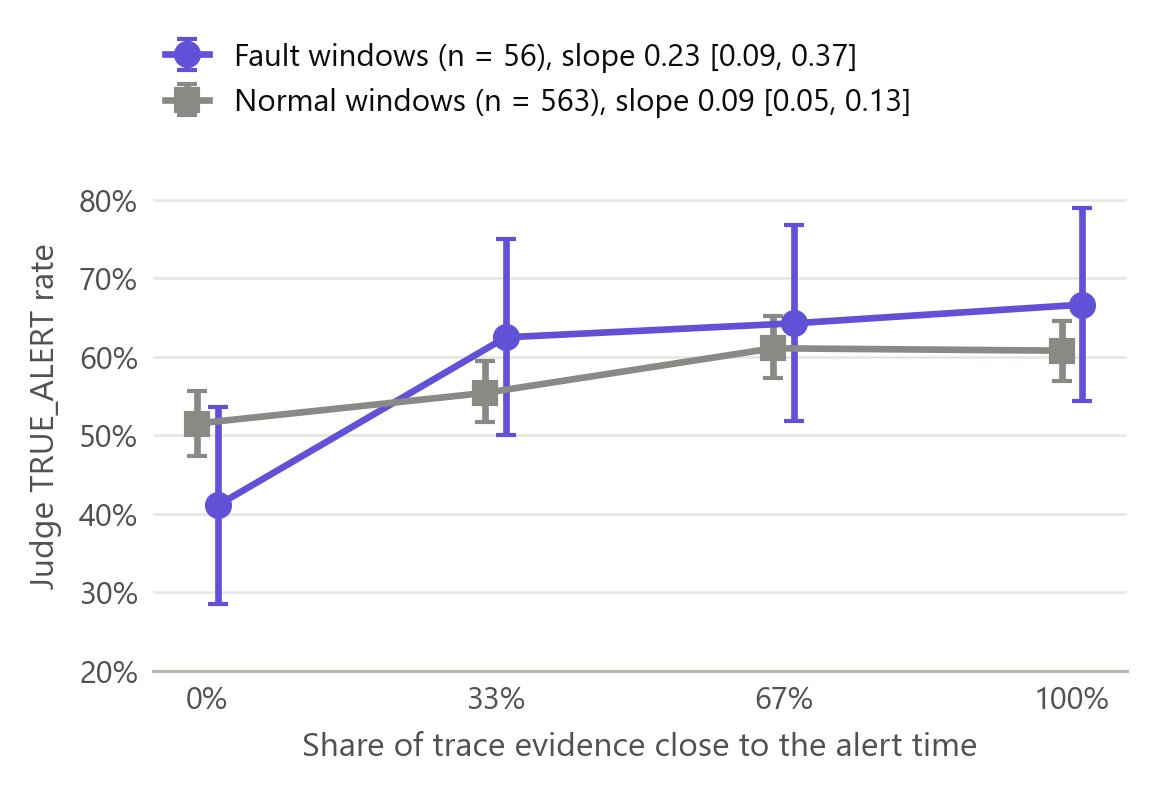
\includegraphics[width=0.92\linewidth]{Images/C1/figures/ch5/h5.4-h1-time-proximity.png}
  \vspace{0.35cm}
  \caption[Kết quả thí nghiệm H1 về độ gần thời gian trên tập val]{Thí nghiệm H1 trên tập \splitname{val}: tỷ lệ judge trả \code{TRUE\_ALERT} tăng đơn điệu theo tỷ lệ bằng chứng trace sát thời điểm $t_0$ ở cả cửa sổ bình thường lẫn cửa sổ lỗi (thanh lỗi: CI95 bootstrap).}
  \label{fig:ch5-h1}
\end{figure}

\begin{table}[htbp]
  \centering
  \caption[Tỷ lệ TRUE\_ALERT thô theo điều kiện can thiệp H1 trên tập val]{Tỷ lệ phán quyết \code{TRUE\_ALERT} thô dưới các điều kiện can thiệp ngữ cảnh trong thí nghiệm H1 trên tập \splitname{val}.}
  \label{tab:ch5-h1}
  \scriptsize
  \renewcommand{\arraystretch}{1.15}
  \begin{tabularx}{\linewidth}{@{}l Y c c@{}}
    \toprule
    \textbf{Điều kiện} & \textbf{Mô tả can thiệp ngữ cảnh} & \textbf{Cửa sổ bình thường [CI95]} & \textbf{Cửa sổ lỗi [CI95]} \\
    \midrule
    \code{ref} & Ngữ cảnh C1 tham chiếu & 0,515 [0,486; 0,543] & 0,505 [0,404; 0,596] \\
    \code{time\_0} / \code{33} / \code{67} & Tỷ lệ trace sát $t_0$ tăng dần & 0,515 / 0,554 / 0,611 & 0,411 / 0,625 / 0,643 \\
    \code{near\_trace} & Chỉ đưa trace span của $s_0$ sát $t_0$ & 0,608 [0,570; 0,646] & 0,667 [0,544; 0,789] \\
    \code{near\_log} & Chỉ đưa log của $s_0$ sát $t_0$ & 0,181 [0,146; 0,215] & 0,211 [0,105; 0,316] \\
    \code{neighbor\_trace} & Chỉ đưa trace span từ service lân cận & 0,277 [0,243; 0,314] & 0,386 [0,263; 0,509] \\
    \bottomrule
  \end{tabularx}
\end{table}

\textbf{H1 được giữ một phần trên tập \splitname{val} (không chạy lại trên \splitname{test}).} Thứ tự liệt kê bằng chứng không tạo khác biệt đo được và điểm hiển thị chỉ có tác động nhỏ ($+0{,}020$, $p = 0{,}062$). Ngược lại, hai yếu tố tác động mạnh nhất là \emph{độ gần thời gian} (độ dốc dương ở cả hai nhãn: $+0{,}094$ $[+0{,}050;\, +0{,}134]$ trên bình thường và $+0{,}230$ $[+0{,}086;\, +0{,}370]$ trên lỗi) và \emph{loại bằng chứng} (trace của chính $s_0$ kích hoạt \code{TRUE\_ALERT} tới $60{,}8\%$ trên cửa sổ bình thường, gấp hơn ba lần so với log cục bộ $18{,}1\%$ và hơn gấp đôi trace lân cận $27{,}7\%$). Điểm quan trọng về mặt phương pháp: vì các yếu tố này làm tăng tỷ lệ xác nhận trên cả hai nhãn (độ nhạy chung của judge với bằng chứng trace sát $t_0$), H1 không cung cấp đặc trưng hồ sơ bằng chứng nào phân tách sạch cửa sổ bình thường khỏi cửa sổ lỗi cho C2 — đây là cơ sở trực tiếp dẫn đến việc chuyển trục thiết kế sang neo bằng chứng bất thường C3.

\subsubsection{Chọn cấu hình \CTAV{} (C3) và loại bỏ C2, C4 trên \splitname{val}}
\label{sec:ch5-val-ctav}

Áp dụng hàm thuần chính sách lên phán quyết đã lưu cache trên \splitname{val}, Bảng~\ref{tab:ch5-val-h3} đối chiếu cấu hình \CTAV{} chốt (C1 + $\theta_{\text{local}} = 0{,}80$ + C3 dùng ngưỡng nền \splitname{dev} $p_{90}$) với từng phép biến đổi một-thay-đổi-một-lần (đường quét ngưỡng $\theta_{\text{topo}}$ chi tiết nằm ở Phụ lục~D). Trên \splitname{val}, bỏ C3 làm cảnh báo sai tăng gần 12 lần ($51 \to 606$ FP) và F1 tụt $-0{,}074$ $[-0{,}124;\, -0{,}027]$; ngược lại, thêm C2 ($\theta_{\text{topo}} = 0{,}85$) chỉ bớt 2 FP ($\Delta\text{FPR} = -0{,}0003$, CI chạm $0$), còn thêm C4 làm chi phí tăng từ $3{,}28$ lên $5{,}14$ USD do tầng 1 BM25 sinh $261$ FP / $15$ TP và tỷ lệ leo thang cao (\textbf{Phát hiện 9}), trong khi F1 giảm nhẹ ($0{,}188$ so với $0{,}201$).

\begin{table}[htbp]
  \centering
  \caption[So sánh các biến thể H3 quanh CTAV trên tập val]{Kết quả lựa chọn cấu hình \CTAV{} và loại trừ từng thành phần trên tập \splitname{val} ($7.636$ cửa sổ có telemetry, $209$ lỗi).}
  \label{tab:ch5-val-h3}
  \scriptsize
  \renewcommand{\arraystretch}{1.15}
  \setlength{\tabcolsep}{3pt}
  \begin{tabularx}{\linewidth}{@{}Y r r r r c r r@{}}
    \toprule
    \textbf{Biến thể trên \splitname{val}} & \textbf{TP} & \textbf{FP} & \textbf{Prec.} & \textbf{Recall} & \textbf{F1 [CI95]} & \textbf{FPR} & \textbf{USD} \\
    \midrule
    \textbf{\CTAV{}} (chốt: C1 + $\theta = 0{,}80$ + C3 \splitname{dev} $p_{90}$) & 29 & 51 & 0,363 & 0,139 & 0,201 [0,138; 0,264] & 0,0069 & 3,28 \\
    + C2 ($\theta_{\text{topo}} = 0{,}85$) & 29 & 49 & 0,372 & 0,139 & 0,202 [0,139; 0,265] & 0,0066 & 3,28 \\
    Bỏ C3 (\code{no\_c3} = C1) & 55 & 606 & 0,083 & 0,263 & 0,126 [0,095; 0,156] & 0,0816 & 3,28 \\
    + C4 (định tuyến hai tầng) & 31 & 90 & 0,256 & 0,148 & 0,188 [0,130; 0,247] & 0,0121 & 5,14 \\
    C3 ngưỡng trượt 60 phút & 34 & 255 & 0,118 & 0,163 & 0,137 [0,097; 0,179] & 0,0343 & 3,28 \\
    \bottomrule
  \end{tabularx}
\end{table}

Dù \CTAV{} đạt F1 sơ bộ cao nhất trên \splitname{val} ($0{,}201$ so với $0{,}103$ của BM25, $\Delta\text{F1} = +0{,}098$ $[+0{,}046;\, +0{,}149]$) và giảm FPR gấp $8$ lần so với BM25, hai giới hạn quan trọng đã được ghi nhận ngay trước khi khóa cấu hình: (i) Recall của \CTAV{} giảm xuống $0{,}139$ so với $0{,}263$ của C1 ($\Delta\text{Recall} = -0{,}124$, \textbf{Phát hiện 10}), và (ii) ngưỡng nền \splitname{dev} $p_{90}$ chỉ phủ $31{,}8\%$--$33{,}2\%$ span trên \splitname{val} do $15$ service không có cửa sổ bình thường trong \splitname{dev} (\textbf{Phát hiện 8}), khiến ưu thế của ngưỡng tĩnh \splitname{dev} một phần đến từ việc im lặng có cấu trúc ở nhóm service thiếu ngưỡng (\textbf{Phát hiện 11}). Theo quy tắc lựa chọn đã ghi trước, cấu hình chốt giữ \splitname{dev} $p_{90}$ và đưa biến thể ngưỡng trượt 60 phút (\code{c3\_rolling\_baseline}, phủ $93\%$ span) vào diện theo dõi bắt buộc trong H3 trên \splitname{test}.

\subsubsection{Khảo sát cổng cứu cảnh báo C5 trên \splitname{val}}
\label{sec:ch5-c5}

Trên tập \splitname{val}, hệ thống tính ngoại tuyến $147$ điểm lưới $(\eta_1, \eta_2, \eta_3, \tau)$ của C5 (\code{Rescue Score}) với tập cảnh báo kích hoạt nhân quả $A$ là $80$ cảnh báo của \CTAV{} trong cửa sổ $300\,\text{s}$ và chấm một lần $1.459$ cửa sổ được cứu ($1{,}03$ USD theo token; đường quét $\tau$ nằm ở Phụ lục~D). Điểm tối ưu trên \splitname{val} là $\eta = (0;\, 0{,}4;\, 0{,}6)$ và $\tau = 0{,}8$ (thành phần log lỗi $\Lambda_{\text{log}}$ không đóng góp vì bằng $0$ ở hầu hết cửa sổ). Bảng~\ref{tab:ch5-val-c5} cho thấy C5 tốn thêm $52$ lượt gọi LLM nhưng chỉ thu thêm $2$ TP trong khi tăng $16$ FP ($\Delta\text{F1} = +0{,}001$ $[-0{,}014;\, +0{,}022]$, $\Delta\text{FPR} = +0{,}0022$ $[+0{,}0011;\, +0{,}0034]$, McNemar $p = 0{,}0013$). Nguyên nhân là nút thắt nằm ở chính bộ thẩm định LLM ($16/21$ cửa sổ lỗi được cứu bị C1 trả \code{FALSE\_POSITIVE}, $3$ ca khác bị C3 hạ, \textbf{Phát hiện 12}). Vì vậy, C5 bị loại khỏi cấu hình \CTAV{} chính và chỉ giữ đúng một điểm cố định cho phép kiểm tra ablation trên \splitname{test}.

\begin{table}[htbp]
  \centering
  \caption[Kết quả cổng cứu cảnh báo C5 trên tập val]{Hiệu quả bổ sung cổng Rescue (C5) tại điểm chọn $\eta = (0;\, 0{,}4;\, 0{,}6)$, $\tau = 0{,}8$ trên tập \splitname{val} ($7.636$ cửa sổ có telemetry, $209$ lỗi).}
  \label{tab:ch5-val-c5}
  \scriptsize
  \renewcommand{\arraystretch}{1.15}
  \begin{tabularx}{\linewidth}{@{}Y r r r r c r@{}}
    \toprule
    \textbf{Cấu hình trên \splitname{val}} & \textbf{+ Lần gọi} & \textbf{TP} & \textbf{FP} & \textbf{Recall} & \textbf{F1 [CI95]} & \textbf{FPR} \\
    \midrule
    \CTAV{} (tắt C5) & 0 & 29 & 51 & 0,139 & 0,201 [0,138; 0,264] & 0,0069 \\
    \CTAV{} + C5 & +52 & 31 & 67 & 0,148 & 0,202 [0,143; 0,261] & 0,0090 \\
    \bottomrule
  \end{tabularx}
\end{table}

% -----------------------------------------------------------------------------
\subsection{Kết quả kiểm định trên tập \splitname{test} (G-test)}
\label{sec:ch5-test}

Sau khi đăng ký toàn bộ giả thuyết và khóa cấu hình tại commit \code{be2b985}, tập \splitname{test} ($46.849$ cửa sổ, trong đó $11.985$ cửa sổ có telemetry và $346$ cửa sổ lỗi) được chạy đúng một lần mà không điều chỉnh bất kỳ tham số nào.

\subsubsection{Giao thức G-test và tổng hợp các lượt chạy}
\label{sec:ch5-test-protocol}

Tất cả cấu hình chạy trên \splitname{test} đều là bản sao nguyên vẹn từ cấu hình \splitname{val}, chỉ thay đổi tên split và mã lượt chạy \code{run\_id}. Bộ thẩm định chấm toàn bộ $13.699$ candidate của \splitname{test} để đảm bảo số liệu đầy đủ cho cả tập chấm chính lẫn tập phụ. Bảng~\ref{tab:ch5-test-runs} tổng hợp toàn bộ các lượt chạy trên \splitname{test}: tổng cộng phát sinh $21.094$ lượt gọi API mới ($15{,}85$ USD theo token) với $0$ lỗi judge. C1 chỉ cần gọi $3.299$ lượt API mới vì $10.400$ candidate không có bằng chứng dùng lại chính xác câu trả lời đã lưu cache của BM25; tương tự, lượt chạy \code{h0\_test\_norag\_v2} tái sử dụng các câu trả lời đã lưu từ cache mà không ghi đè thư mục cũ.

\begin{table}[htbp]
  \centering
  \caption[Danh sách các lượt chạy kiểm định trên tập test]{Tổng hợp các lượt chạy chính thức của cổng G-test trên tập \splitname{test} ($46.849$ cửa sổ, $13.699$ candidate).}
  \label{tab:ch5-test-runs}
  \scriptsize
  \renewcommand{\arraystretch}{1.15}
  \setlength{\tabcolsep}{3pt}
  \begin{tabularx}{\linewidth}{@{}l Y r r r r@{}}
    \toprule
    \textbf{Mã lượt chạy (\code{run\_id})} & \textbf{Nội dung} & \textbf{Lượt gọi LLM} & \textbf{API mới} & \textbf{Lỗi} & \textbf{USD mới} \\
    \midrule
    \code{m8\_test\_detector\_count\_v1} & Chỉ detector (đếm candidate) & 0 & 0 & -- & 0,00 \\
    \code{h0\_test\_bm25\_v1} & BM25 + judge & 13.699 & 13.699 & 0 & 8,87 \\
    \code{h0\_test\_c1\_k0\_v1} & C1 + judge & 13.699 & 3.299 & 0 & 4,71 \\
    \code{h0\_test\_norag\_v2} & LLM-không-RAG (kế tiếp cache \code{\_v1}) & 13.699 & 3.287 & 0 & 1,10 \\
    \code{h0\_test\_*\_b120\_v1} & Ba lượt ngân sách 120 lần gọi & $3 \times 120$ & 0 & 0 & 0,00 \\
    \code{ctav\_final\_test\_v1} & Replay \CTAV{} + 4 nhánh ablation & 0 (replay) & 0 & -- & 0,00 \\
    \code{m8\_rescue\_test\_c1\_v1} & C5 một điểm (cửa sổ được cứu) & 61 & 61 & 0 & 0,09 \\
    \code{h0\_test\_*\_rep\{1,2\}\_v1} & Đo phương sai judge ($4 \times 200$ cửa sổ) & 800 & 748 & 0 & 1,08 \\
    \midrule
    \textbf{Tổng G-test} & & & \textbf{21.094} & \textbf{0} & \textbf{15,85} \\
    \bottomrule
  \end{tabularx}
\end{table}

\subsubsection{Hành vi bộ phát hiện trên \splitname{test} và độ lệch giữa các split}
\label{sec:ch5-test-shift}

Trước khi đọc các chỉ số so sánh, cần nắm rõ phân bố ứng viên đầu vào đã dịch chuyển giữa các split dù ngưỡng Isolation Forest ($0{,}85$) không đổi (Hình~\ref{fig:ch5-shift} và Bảng~\ref{tab:ch5-shift}). Theo cách chuẩn hóa phân vị trên \splitname{dev}, tỷ lệ candidate trên \splitname{dev} đúng bằng $15{,}0\%$; sang \splitname{val} tăng lên $19{,}6\%$ và sang \splitname{test} đạt $29{,}2\%$ ($13.699 / 46.849$ cửa sổ).

\begin{figure}[htbp]
  \centering
  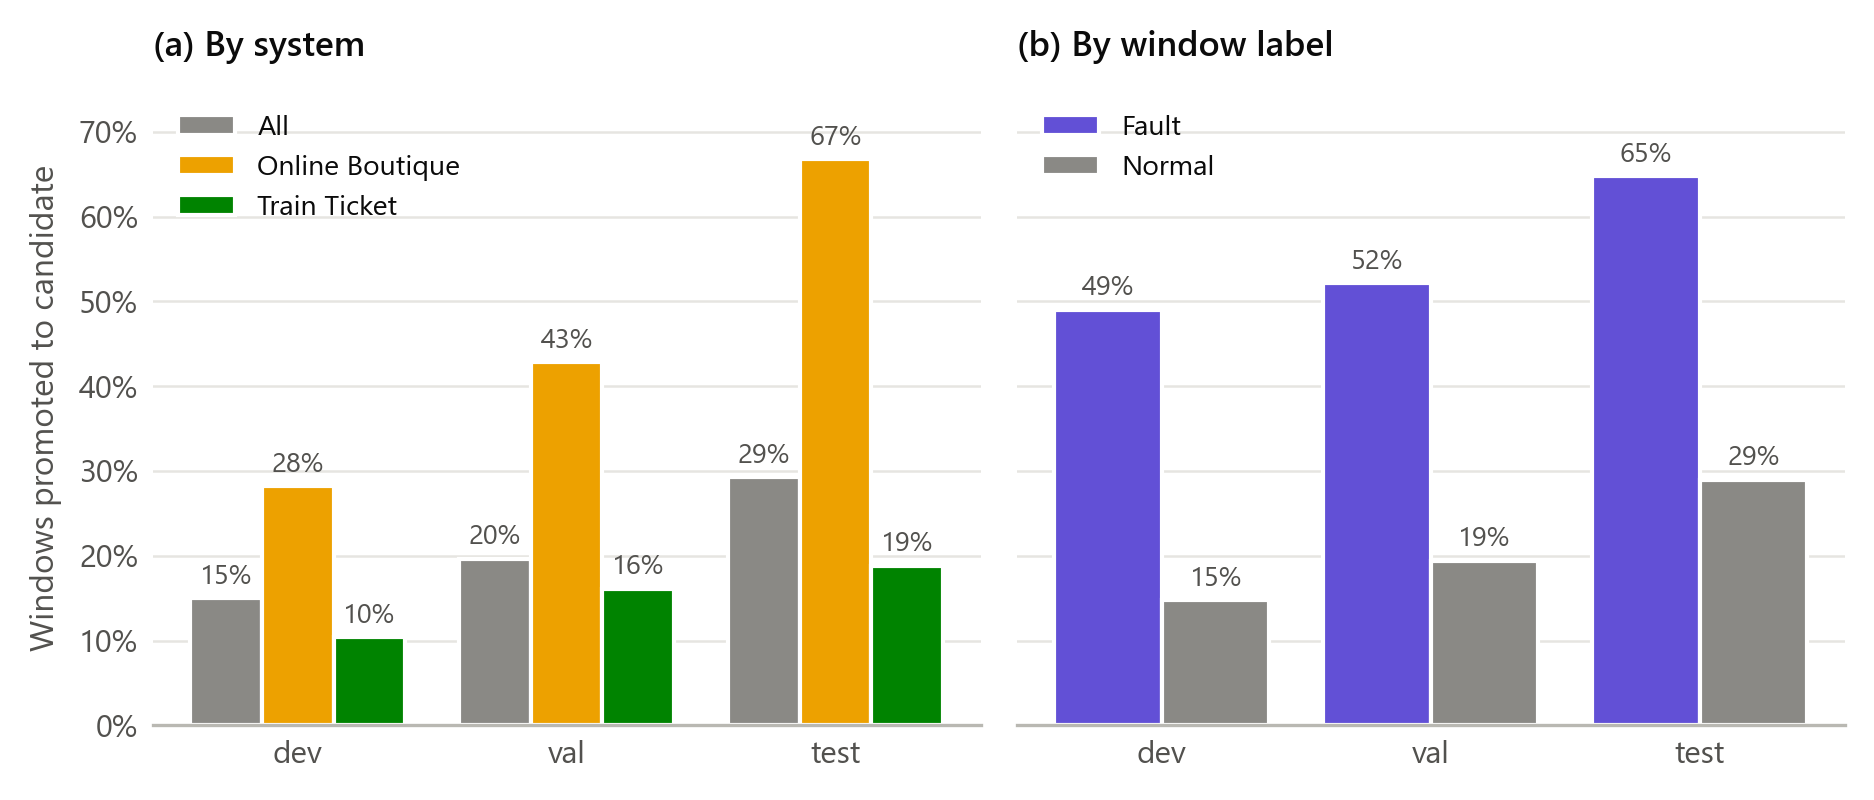
\includegraphics[width=0.92\linewidth]{Images/C1/figures/ch5/h5.8-candidate-rate-by-split.png}
  \vspace{0.35cm}
  \caption[Tỷ lệ candidate của detector trên ba split dev, val và test]{Tỷ lệ cửa sổ trở thành candidate ($\text{score}_{\text{IF}} \ge 0{,}85$) trên \splitname{dev}, \splitname{val}, \splitname{test}: (a)~theo hệ thống và (b)~theo nhãn cửa sổ.}
  \label{fig:ch5-shift}
\end{figure}

\begin{table}[htbp]
  \centering
  \caption[So sánh hành vi bộ phát hiện đã đóng băng trên ba split]{Thống kê bộ phát hiện Isolation Forest (ngưỡng $0{,}85$, huấn luyện trên \splitname{dev}) qua ba split \splitname{dev}, \splitname{val} và \splitname{test}.}
  \label{tab:ch5-shift}
  \scriptsize
  \renewcommand{\arraystretch}{1.15}
  \begin{tabularx}{\linewidth}{@{}Y r r r@{}}
    \toprule
    \textbf{Chỉ tiêu} & \textbf{\splitname{dev}} & \textbf{\splitname{val}} & \textbf{\splitname{test}} \\
    \midrule
    Tổng cửa sổ & 19.316 & 28.898 & 46.849 \\
    Số candidate (tỷ lệ) & 2.898 (15,0\%) & 5.677 (19,6\%) & 13.699 (29,2\%) \\
    Điểm bất thường trung vị / p90 & 0,500 / 0,900 & 0,549 / 0,910 & 0,588 / 0,953 \\
    Recall detector-only & 73 / 149 (0,490) & 109 / 209 (0,522) & 224 / 346 (0,647) \\
    FPR detector-only (có telemetry) & 825 / 4.881 (0,1693) & 1.640 / 7.427 (0,2208) & 3.435 / 11.639 (0,2951) \\
    OnlineBoutique: tỷ trọng split; tỷ lệ candidate & 25,8\%; 28,2\% & 13,2\%; 42,8\% & 21,8\%; 66,8\% \\
    TrainTicket: tỷ lệ candidate & 10,4\% & 16,1\% & 18,8\% \\
    Số service ``luôn bật'' ($\ge 90\%$ candidate) & 2 & 3 & 5 \\
    \bottomrule
  \end{tabularx}
\end{table}

Độ lệch này không xuất phát từ một ngày đơn lẻ mà đến từ thành phần service của từng split khi chia theo lần tiêm lỗi: \splitname{test} có tỷ trọng cửa sổ OnlineBoutique cao hơn \splitname{val} ($21{,}8\%$ so với $13{,}2\%$) với tỷ lệ candidate tới $66{,}8\%$, trong đó năm service gần như luôn vượt ngưỡng (\code{checkoutservice}, \code{currencyservice}, \code{frontend}, \code{productcatalogservice}, \code{ts-ui-dashboard}) tạo ra $6.407$ candidate ($47\%$ toàn bộ \splitname{test}; riêng \code{frontend} không xuất hiện ở \splitname{val}). Ba hệ quả trực tiếp cần lưu ý khi đọc kết quả phía sau: (i) bộ phát hiện trên \splitname{test} có cả Recall ($0{,}647$) lẫn FPR ($0{,}2951$) cao hơn \splitname{val}; (ii) mốc $4.000$ lần gọi trên đường ngân sách chỉ phủ $29\%$ candidate của \splitname{test} và nằm trọn trong ngày đầu tiên của OnlineBoutique; và (iii) chi phí chấm toàn bộ \splitname{test} cao gấp $2{,}4$ lần \splitname{val}.

\subsubsection{Bức tranh tổng quan các phương pháp trên \splitname{test}}
\label{sec:ch5-test-overview}

Bảng~\ref{tab:ch5-test-overview} và Hình~\ref{fig:ch5-operating} đặt năm phương pháp trên mặt phẳng Recall--FPR của tập chấm chính (\splitname{test}: $11.985$ cửa sổ có telemetry, $346$ lỗi) cạnh các điểm tham chiếu trên \splitname{val}. Thứ tự trên trục FPR được bảo toàn tuyệt đối giữa hai split: $\text{\CTAV} < \text{BM25} \approx \text{không-RAG} < \text{C1} < \text{detector-only}$. Cụ thể, \CTAV{} đạt FPR thấp nhất toàn bảng ($0{,}0055$, chỉ $64$ cảnh báo sai trên $11.639$ cửa sổ bình thường) và Precision cao nhất ($0{,}179$), nhưng Recall giảm xuống còn $0{,}040$ ($14$ TP) khiến F1 hạ từ $0{,}201$ trên \splitname{val} xuống $0{,}066$ trên \splitname{test}. Ở chiều ngược lại, trên tập phụ gồm mọi cửa sổ ($46.849$ cửa sổ), BM25, C1 và \CTAV{} giữ nguyên số TP/FP nhờ luật \code{require\_evidence}, còn LLM-không-RAG sinh thêm $832$ cảnh báo sai trên vùng không có telemetry (tổng $1.203$ FP, F1 tụt còn $0{,}047$).

\begin{figure}[htbp]
  \centering
  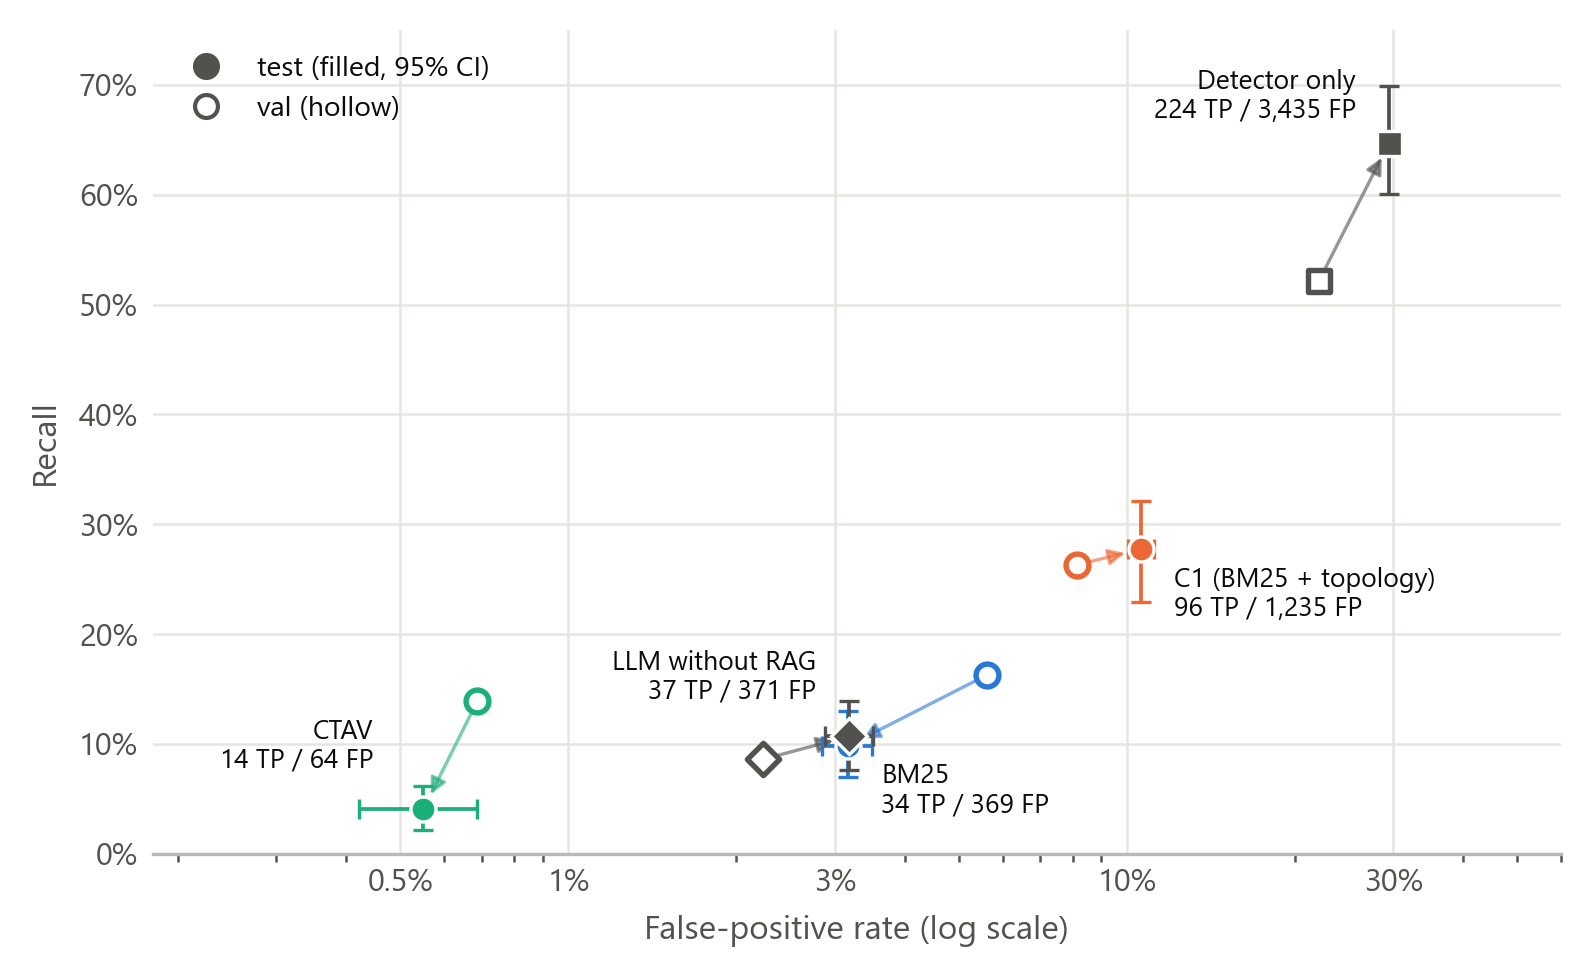
\includegraphics[width=0.92\linewidth]{Images/C1/figures/ch5/h5.9-recall-fpr-operating-points.png}
  \vspace{0.35cm}
  \caption[Điểm vận hành Recall--FPR của năm phương pháp trên val và test]{Điểm vận hành Recall--FPR (trục FPR thang log) trên cửa sổ có telemetry của \splitname{val} (điểm rỗng) và \splitname{test} (điểm đặc kèm CI95 và nhãn TP/FP).}
  \label{fig:ch5-operating}
\end{figure}

\begin{table}[htbp]
  \centering
  \caption[So sánh tổng quan năm phương pháp trên test cạnh val]{Hiệu năng năm phương pháp trên \splitname{test} (cửa sổ có telemetry: $11.985$ cửa sổ, $346$ lỗi) cạnh tham chiếu \splitname{val} ($7.636$ cửa sổ, $209$ lỗi).}
  \label{tab:ch5-test-overview}
  \scriptsize
  \renewcommand{\arraystretch}{1.15}
  \setlength{\tabcolsep}{2.5pt}
  \begin{tabularx}{\linewidth}{@{}Y r r r c c c r@{}}
    \toprule
    \textbf{Phương pháp} & \textbf{TP} & \textbf{FP} & \textbf{Prec.} & \textbf{Recall [CI95]} & \textbf{F1 [CI95]} & \textbf{FPR [CI95]} & \textbf{\splitname{val} F1} \\
    \midrule
    Detector-only & 224 & 3.435 & 0,061 & 0,647 [0,601; 0,699] & 0,112 [0,100; 0,126] & 0,2951 [0,2870; 0,3036] & 0,111 \\
    LLM-không-RAG & 37 & 371 & 0,091 & 0,107 [0,077; 0,139] & 0,098 [0,071; 0,126] & 0,0319 [0,0288; 0,0351] & 0,092 \\
    BM25 & 34 & 369 & 0,084 & 0,098 [0,070; 0,130] & 0,091 [0,064; 0,119] & 0,0317 [0,0285; 0,0350] & 0,103 \\
    C1 ($k_{\text{graph}} = 0$) & 96 & 1.235 & 0,072 & 0,277 [0,230; 0,321] & 0,114 [0,093; 0,135] & 0,1061 [0,1007; 0,1118] & 0,126 \\
    \textbf{\CTAV{}} (\splitname{dev} $p_{90}$) & \textbf{14} & \textbf{64} & \textbf{0,179} & \textbf{0,040 [0,022; 0,061]} & \textbf{0,066 [0,036; 0,100]} & \textbf{0,0055 [0,0042; 0,0069]} & 0,201 \\
    \midrule
    \emph{Đối chứng H3:} C3-trượt & 47 & 391 & 0,107 & 0,136 [0,101; 0,172] & 0,120 [0,090; 0,151] & 0,0336 [0,0304; 0,0369] & 0,137 \\
    \bottomrule
  \end{tabularx}
\end{table}

\subsubsection{Kiểm định H0: topology chưa hiệu chỉnh tăng recall và FPR}
\label{sec:ch5-test-h0}

Giả thuyết H0 kiểm tra liệu truy xuất nhận biết topology chưa hiệu chỉnh (C1) có làm tăng đồng thời Recall và FPR so với BM25 trên tập \splitname{test} hay không. Theo bản đăng ký, H0 chỉ được chấp nhận khi đạt cả bốn vế: CI95 của $\Delta\text{Recall}(\text{C1}-\text{BM25})$ có cận dưới $> 0$, CI95 của $\Delta\text{FPR}(\text{C1}-\text{BM25})$ có cận dưới $> 0$, và kiểm định McNemar trên cả cửa sổ lỗi lẫn cửa sổ bình thường đều cho $p < 0{,}05$ (Bảng~\ref{tab:ch5-test-h0}).

\begin{table}[htbp]
  \centering
  \caption[Kiểm định giả thuyết H0 trên tập test]{Kết quả kiểm định H0 (C1 $-$ BM25) trên tập \splitname{test} ($11.985$ cửa sổ có telemetry, $346$ lỗi) cạnh tham chiếu \splitname{val}.}
  \label{tab:ch5-test-h0}
  \scriptsize
  \renewcommand{\arraystretch}{1.15}
  \setlength{\tabcolsep}{3pt}
  \begin{tabularx}{\linewidth}{@{}Y >{\raggedright\arraybackslash}p{4.6cm} l >{\raggedright\arraybackslash}p{3.1cm}@{}}
    \toprule
    \textbf{Vế tiêu chí H0} & \textbf{Số đo trên \splitname{test}} & \textbf{Kết quả} & \textbf{\splitname{val} (tham chiếu)} \\
    \midrule
    CI95 $\Delta\text{Recall}(\text{C1}-\text{BM25})$ cận dưới $> 0$ & $+0{,}179$ $[+0{,}138;\, +0{,}226]$ & \textbf{Đạt} & $+0{,}100$ $[+0{,}052;\, +0{,}155]$ \\
    CI95 $\Delta\text{FPR}(\text{C1}-\text{BM25})$ cận dưới $> 0$ & $+0{,}0744$ $[+0{,}0694;\, +0{,}0798]$ & \textbf{Đạt} & $+0{,}0254$ $[+0{,}0204;\, +0{,}0306]$ \\
    McNemar cửa sổ lỗi, $p < 0{,}05$ & $p < 0{,}001$ (C1 đúng/BM25 sai: 65; ngược lại: 3) & \textbf{Đạt} & $p < 0{,}001$ (28; 7) \\
    McNemar cửa sổ bình thường, $p < 0{,}05$ & $p < 0{,}001$ (BM25 đúng/C1 sai: 966; ngược lại: 100) & \textbf{Đạt} & $p < 0{,}001$ (276; 87) \\
    \emph{Phụ:} $\Delta\text{F1}$ (ngoài tiêu chí) & $+0{,}024$ $[-0{,}001;\, +0{,}052]$ & -- & $+0{,}023$ $[-0{,}004;\, +0{,}052]$ \\
    \bottomrule
  \end{tabularx}
\end{table}

\textbf{H0 được chấp nhận trên tập \splitname{test} (đạt 4/4 vế).} So với BM25, C1 bắt thêm $62$ cửa sổ lỗi ($96$ so với $34$ TP; có $65$ cửa sổ lỗi C1 bắt đúng mà BM25 bỏ sót, chiều ngược lại chỉ $3$) nhưng đồng thời tạo thêm $866$ cảnh báo sai ($1.235$ so với $369$ FP; FPR tăng gấp $3{,}3$ lần). So với \splitname{val}, hiện tượng lặp lại với biên độ lớn hơn ở cả hai chiều, trong khi CI95 của $\Delta\text{F1}$ tiếp tục chứa $0$ ($[-0{,}001;\, +0{,}052]$). Lưu ý rằng H0 kiểm định hiện tượng đầu ra; cơ chế gây nhiễu đã được khảo sát ở H1 trên \splitname{val} và không chạy lại trên \splitname{test}.

\subsubsection{Kiểm định H2: \CTAV{} so với BM25 và C1 (giả thuyết chính)}
\label{sec:ch5-test-h2}

Giả thuyết chính H2 kiểm tra liệu cấu hình \CTAV{} đã đóng băng có đạt đồng thời ba vế tiêu chí đã đăng ký hay không: (i)~CI95 của $\Delta\text{F1}(\text{\CTAV}-\text{BM25})$ có cận dưới $> 0$ và McNemar $p < 0{,}05$; (ii)~CI95 của $\Delta\text{FPR}(\text{\CTAV}-\text{BM25})$ không có cận dưới $> 0$; và (iii)~ước lượng điểm $\Delta\text{Recall}(\text{\CTAV}-\text{C1}) \ge -0{,}05$. Hình~\ref{fig:ch5-forest} trực quan hóa toàn bộ các hiệu ghép cặp và CI95 trên cả hai split, còn Bảng~\ref{tab:ch5-test-h2} đối chiếu từng vế tiêu chí của H2.

\begin{figure}[htbp]
  \centering
  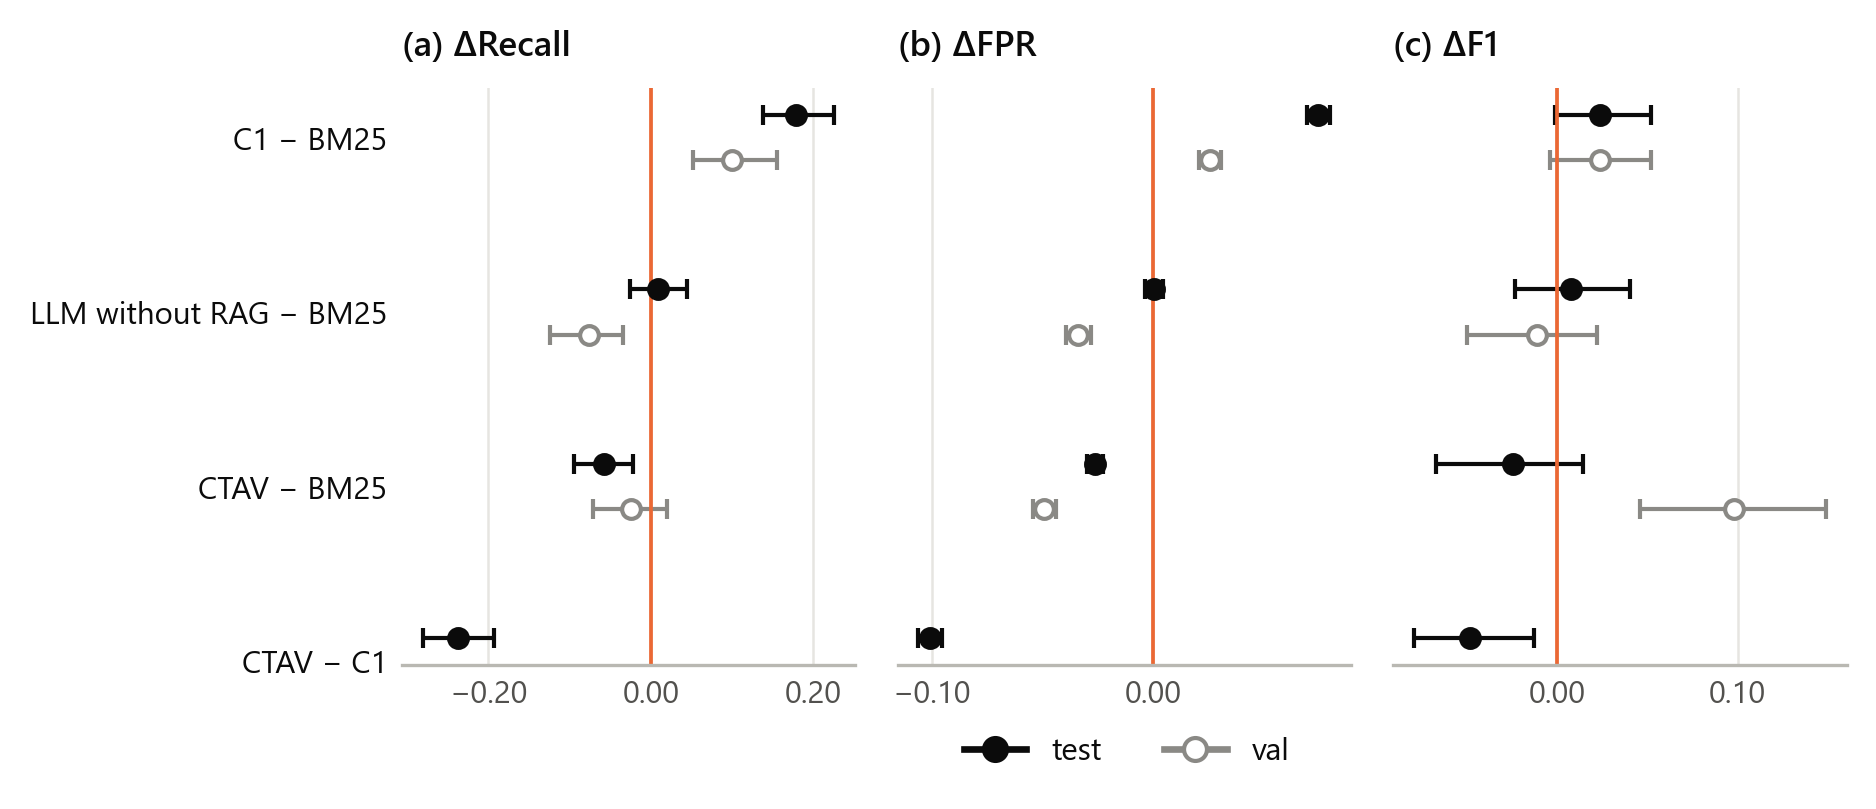
\includegraphics[width=\linewidth]{Images/C1/figures/ch5/h5.10-paired-differences-ci.png}
  \vspace{0.35cm}
  \caption[Hiệu ghép cặp và khoảng tin cậy CI95 của các phương pháp]{Hiệu ghép cặp $\Delta\text{Recall}$, $\Delta\text{FPR}$ và $\Delta\text{F1}$ kèm CI95 bootstrap trên \splitname{test} (điểm đặc) và \splitname{val} (điểm rỗng); vạch dọc tại $0$ giúp nhận diện ngay vế có ý nghĩa thống kê.}
  \label{fig:ch5-forest}
\end{figure}

\begin{table}[htbp]
  \centering
  \caption[Kiểm định giả thuyết chính H2 trên tập test]{Kết quả kiểm định H2 trên tập \splitname{test} ($11.985$ cửa sổ có telemetry, $346$ lỗi) cạnh tham chiếu \splitname{val}.}
  \label{tab:ch5-test-h2}
  \scriptsize
  \renewcommand{\arraystretch}{1.15}
  \setlength{\tabcolsep}{3pt}
  \begin{tabularx}{\linewidth}{@{}Y l >{\raggedright\arraybackslash}p{4.1cm} l >{\raggedright\arraybackslash}p{2.6cm}@{}}
    \toprule
    \textbf{Vế tiêu chí H2} & \textbf{So sánh} & \textbf{Số đo trên \splitname{test}} & \textbf{Kết quả} & \textbf{\splitname{val} (sơ bộ)} \\
    \midrule
    (i) CI95 $\Delta\text{F1}$ cận dưới $> 0$ \& McNemar $p < 0{,}05$ & \CTAV{} $-$ BM25 & $-0{,}025$ $[-0{,}067;\, +0{,}014]$; $p < 0{,}001$ & \textbf{Không đạt} & $+0{,}098$ $[+0{,}046;\, +0{,}149]$ \\
    (ii) CI95 $\Delta\text{FPR}$ không có cận dưới $> 0$ & \CTAV{} $-$ BM25 & $-0{,}0262$ $[-0{,}0297;\, -0{,}0229]$ & \textbf{Đạt} & $-0{,}0493$ $[-0{,}0545;\, -0{,}0439]$ \\
    (iii) $\Delta\text{Recall} \ge -0{,}05$ (ước lượng điểm) & \CTAV{} $-$ C1 & $-0{,}237$ $[-0{,}281;\, -0{,}193]$ & \textbf{Không đạt} & $-0{,}124$ (không đạt) \\
    \emph{Phụ:} $\Delta\text{Precision}$ & \CTAV{} $-$ BM25 & $+0{,}095$ $[+0{,}014;\, +0{,}186]$ & -- & $+0{,}279$ \\
    \emph{Phụ:} $\Delta\text{Recall}$ & \CTAV{} $-$ BM25 & $-0{,}058$ $[-0{,}095;\, -0{,}022]$ & -- & $-0{,}024$ \\
    \emph{Phụ:} $\Delta\text{F1}$ & \CTAV{} $-$ C1 & $-0{,}048$ $[-0{,}079;\, -0{,}013]$ & -- & $+0{,}074$ \\
    \emph{Phụ:} $\Delta\text{F1}$ & \CTAV{} $-$ không-RAG & $-0{,}032$ $[-0{,}075;\, +0{,}008]$ & -- & $+0{,}109$ \\
    \bottomrule
  \end{tabularx}
\end{table}

\textbf{H2 không được chấp nhận trên tập \splitname{test}.} Theo số đếm trên $11.985$ cửa sổ có telemetry, vế (ii) đạt rất rõ rệt: \CTAV{} loại $305$ cảnh báo sai so với BM25 ($369 \to 64$ FP, giảm $5{,}8$ lần) và loại $1.171$ cảnh báo sai so với C1 ($1.235 \to 64$ FP, giảm $94{,}8\%$), nâng Precision hơn gấp đôi so với BM25 ($0{,}179$ so với $0{,}084$, $\Delta\text{Precision} = +0{,}095$ $[+0{,}014;\, +0{,}186]$). Tuy nhiên, bộ lọc C3 dùng ngưỡng tĩnh \splitname{dev} đồng thời làm rơi $82 / 96$ TP của C1 (còn $14$ TP, thấp hơn $34$ TP của BM25; McNemar riêng trên cửa sổ lỗi $p = 0{,}004$), khiến cả vế (iii) ($\Delta\text{Recall} = -0{,}237 < -0{,}05$) lẫn vế (i) ($\Delta\text{F1} = -0{,}025$ $[-0{,}067;\, +0{,}014]$, CI chứa $0$) đều không đạt. So với \splitname{val}, mức giảm FPR nhất quán ($0{,}0069 \to 0{,}0055$), nhưng mức hụt recall so với C1 tăng gần gấp đôi ($-0{,}124 \to -0{,}237$), chuyển kết luận từ ``đạt một phần'' trên \splitname{val} thành ``không được chấp nhận'' trên \splitname{test}. Nguyên nhân cốt lõi (độ phủ ngưỡng nền \splitname{dev}) được định lượng chi tiết ở Mục~\ref{sec:ch5-finding11}.

\subsubsection{Kiểm định H3: đóng góp của từng thành phần}
\label{sec:ch5-test-h3}

Giả thuyết H3 kiểm định vai trò của từng thành phần quanh \CTAV{} bằng phương pháp một-thay-đổi-một-lần theo ba tiêu chí đăng ký (Bảng~\ref{tab:ch5-test-h3}): bỏ C3 phải làm CI95 của $\Delta\text{Precision}$ có cận trên $< 0$; thêm lại C2 ($\theta_{\text{topo}} = 0{,}85$) xác nhận quyết định loại nếu CI95 $\Delta\text{FPR}$ chứa $0$ hoặc $> 0$; và thêm lại C4 xác nhận quyết định loại nếu chi phí tăng mà CI95 $\Delta\text{F1}$ không có cận dưới $> 0$. Hai biến thể C3-trượt và C5 một điểm được báo mô tả kèm theo.

\begin{table}[htbp]
  \centering
  \caption[Kiểm định giả thuyết H3 trên tập test]{Kết quả kiểm định H3 theo từng thành phần trên tập \splitname{test} ($11.985$ cửa sổ có telemetry, $346$ lỗi).}
  \label{tab:ch5-test-h3}
  \scriptsize
  \renewcommand{\arraystretch}{1.15}
  \setlength{\tabcolsep}{3pt}
  \begin{tabularx}{\linewidth}{@{}l Y >{\raggedright\arraybackslash}p{4.2cm} l@{}}
    \toprule
    \textbf{Thành phần} & \textbf{Tiêu chí đã đăng ký} & \textbf{Số đo trên \splitname{test}} & \textbf{Kết quả} \\
    \midrule
    C3 (đang dùng) & Bỏ C3 $\Rightarrow$ CI95 $\Delta\text{Precision}$ cận trên $< 0$ & $-0{,}107$ $[-0{,}197;\, -0{,}030]$ & \textbf{Đạt} (đóng góp) \\
    C2 (đã loại) & Thêm C2: CI95 $\Delta\text{FPR}$ chứa $0$ hoặc $> 0$ & $+0{,}0000$ $[+0{,}0000;\, +0{,}0000]$ & \textbf{Đạt} (xác nhận loại) \\
    C4 (đã loại) & Thêm C4: chi phí tăng \& CI95 $\Delta\text{F1}$ không có cận dưới $> 0$ & $-0{,}001$ $[-0{,}001;\, +0{,}000]$; $13{,}56$ vs $8{,}16$ USD & \textbf{Đạt} (xác nhận loại) \\
    C3-trượt & Báo mô tả $\Delta\text{F1}$, $\Delta\text{FPR}$, $\Delta\text{Recall}$ & $\Delta\text{F1} = +0{,}054$ $[+0{,}017;\, +0{,}091]$; $\Delta\text{FPR} = +0{,}0281$; $\Delta\text{Recall} = +0{,}095$ & Mô tả \\
    C5 một điểm & Báo mô tả $\Delta\text{Recall}$, $\Delta\text{FPR}$, +lần gọi & $\Delta\text{Recall} = +0{,}000$; $\Delta\text{FPR} = +0{,}0001$; $+61$ lần gọi & Mô tả \\
    \bottomrule
  \end{tabularx}
\end{table}

\textbf{H3 được chấp nhận trên tập \splitname{test} (đạt cả ba tiêu chí thành phần).} Khi bỏ C3, báo động sai nhảy từ $64$ lên $1.235$ FP làm Precision tụt $0{,}107$; thêm lại C2 không thay đổi một phán quyết cuối nào ($0$ TP, $0$ FP thay đổi vì toàn bộ $54$ ca bị C2 hạ đều đã bị C3 hạ trước đó); còn thêm lại C4 tiêu tốn thêm $3.286$ lượt gọi LLM ($13{,}56$ so với $8{,}16$ USD quy đổi cả cache) và thêm $4$ FP mà không thêm TP nào. Đối chiếu với \splitname{val}, cả ba quyết định giữ C3 và loại C2, C4 đều nhất quán hoàn toàn; điểm đảo chiều duy nhất là biến thể \code{C3-trượt} tăng thêm $33$ TP ($14 \to 47$ TP) và nâng F1 thêm $+0{,}054$ $[+0{,}017;\, +0{,}091]$ lên $0{,}120$, khẳng định sự khác biệt nằm ở cách ước lượng ngưỡng nền.

\subsubsection{Kiểm định H4: hiệu quả ở ngân sách nhỏ 120 lần gọi}
\label{sec:ch5-h4}

Giả thuyết H4 kiểm tra điều kiện ngân sách hạn hẹp ở $120$ lượt gọi LLM đầu tiên theo thứ tự thời gian, với tiêu chí đăng ký là ước lượng điểm $\text{F1}(\text{\CTAV}) \ge \text{F1}(\text{LLM-không-RAG})$ (Bảng~\ref{tab:ch5-test-h4}).

\begin{table}[htbp]
  \centering
  \caption[Kiểm định giả thuyết H4 ở ngân sách 120 lần gọi trên test]{So sánh bốn phương pháp ở ngân sách 120 lượt gọi LLM đầu tiên trên \splitname{test} ($11.985$ cửa sổ có telemetry, $346$ lỗi) cạnh tham chiếu \splitname{val}.}
  \label{tab:ch5-test-h4}
  \scriptsize
  \renewcommand{\arraystretch}{1.15}
  \begin{tabularx}{\linewidth}{@{}Y r r r r c r@{}}
    \toprule
    \textbf{Phương pháp} & \textbf{TP} & \textbf{FP} & \textbf{Precision} & \textbf{Recall} & \textbf{F1 [CI95] (\splitname{test})} & \textbf{F1 (\splitname{val})} \\
    \midrule
    \textbf{\CTAV{}} & 6 & 0 & 1,000 & 0,017 & \textbf{0,034 [0,011; 0,064]} & 0,028 \\
    LLM-không-RAG & 3 & 3 & 0,500 & 0,009 & 0,017 [0,000; 0,038] & 0,000 \\
    BM25 & 3 & 3 & 0,500 & 0,009 & 0,017 [0,000; 0,038] & 0,016 \\
    C1 & 11 & 23 & 0,324 & 0,032 & 0,058 [0,026; 0,092] & 0,023 \\
    \bottomrule
  \end{tabularx}
\end{table}

\textbf{H4 được chấp nhận trên tập \splitname{test}.} Trong $120$ candidate đầu tiên, \CTAV{} bắt $6$ TP với $0$ FP ($\text{Precision} = 1{,}000$, $\text{F1} = 0{,}034$), gấp đôi số TP của LLM-không-RAG và BM25 (cùng $3$ TP, $3$ FP, $\text{F1} = 0{,}017$), trùng chiều quan sát trên \splitname{val} ($0{,}028$ so với $0{,}000$). Tuy nhiên, cần đọc kèm hai giới hạn: $120$ lượt gọi chỉ bằng $0{,}9\%$ tổng số candidate của \splitname{test} khiến CI95 chồng nhau rộng giữa hai phương pháp, và toàn bộ $120$ candidate đầu thuộc đầu ngày OnlineBoutique nơi \code{frontend} có sẵn ngưỡng \splitname{dev}.

\subsubsection{Bảng tổng hợp kết quả kiểm định H0--H5}
\label{sec:ch5-test-summary}

Bảng~\ref{tab:ch5-verdict-summary} tổng hợp toàn bộ kết luận kiểm định chính thức của sáu giả thuyết H0--H5 trên \splitname{test} đặt cạnh kết quả sơ bộ trên \splitname{val} (kết quả chi tiết H5 được trình bày ở Mục~\ref{sec:ch5-rca}).

\begin{table}[htbp]
  \centering
  \caption[Tổng hợp kết luận kiểm định H0--H5 trên test và val]{Tổng hợp kết luận kiểm định chính thức của các giả thuyết H0--H5 trên tập \splitname{test} so với kết quả sơ bộ trên \splitname{val}.}
  \label{tab:ch5-verdict-summary}
  \scriptsize
  \renewcommand{\arraystretch}{1.15}
  \setlength{\tabcolsep}{3pt}
  \begin{tabularx}{\linewidth}{@{}l >{\raggedright\arraybackslash}p{2.3cm} Y >{\raggedright\arraybackslash}p{3.0cm}@{}}
    \toprule
    \textbf{Giả thuyết} & \textbf{So sánh} & \textbf{Kết luận chính thức trên \splitname{test}} & \textbf{Kết quả sơ bộ trên \splitname{val}} \\
    \midrule
    \textbf{H0} & C1 $-$ BM25 & \textbf{Được chấp nhận} (đạt 4/4 vế) & Được chấp nhận \\
    \textbf{H1} & Can thiệp mẫu cố định & \emph{Không chạy lại trên \splitname{test}} & Giữ một phần \\
    \textbf{H2} (chính) & \CTAV{} $-$ BM25, $-$ C1 & \textbf{Không được chấp nhận} (đạt vế (ii) FPR; không đạt vế (i) F1 và vế (iii) Recall) & Đạt một phần \\
    \textbf{H3} & Ablation quanh \CTAV{} & \textbf{Được chấp nhận} (C3 đóng góp; xác nhận loại C2, C4; C3-trượt $\Delta\text{F1}=+0{,}054$; C5 $+0$ TP) & C3 đóng góp; xác nhận loại C2, C4 \\
    \textbf{H4} & Ngân sách 120 lần gọi & \textbf{Được chấp nhận} ($0{,}034 \ge 0{,}017$; CI chồng nhau) & Đạt ($0{,}028$ vs $0{,}000$) \\
    \textbf{H5} & Tác tử RCA & \textbf{Không được chấp nhận} (0/4 vế: $\text{Hit@1}=\text{Hit@3}=0{,}471=\text{baseline}$, 0 cascade) & Không đạt đầy đủ \\
    \bottomrule
  \end{tabularx}
\end{table}

% -----------------------------------------------------------------------------
\subsection{Phân tích thành phần, cơ chế và đường cong trên \splitname{test}}
\label{sec:ch5-ablation}

Trong khi Mục~\ref{sec:ch5-test} trả lời câu hỏi giả thuyết nào đạt hay không đạt, mục này mổ xẻ các cơ chế định lượng đứng sau kết quả trên \splitname{test}.

\subsubsection{Phễu quyết định và ablation thành phần (\splitname{val} cạnh \splitname{test})}
\label{sec:ch5-ablation-detail}

Hình~\ref{fig:ch5-funnel} mô tả phễu lọc của \CTAV{} trên $11.985$ cửa sổ có telemetry của \splitname{test}: bộ phát hiện giữ $3.659$ candidate ($224$ lỗi, $3.435$ bình thường); bộ thẩm định trên ngữ cảnh C1 trả \code{TRUE\_ALERT} thô cho $1.418$ cửa sổ ($96$ lỗi, $1.322$ bình thường); luật \code{require\_evidence} hạ $87$ cửa sổ bình thường không có trích dẫn hợp lệ (ngưỡng $\theta_{\text{local}} = 0{,}80$ hạ $0$ cửa sổ), để lại $1.331$ cảnh báo của C1 ($96$ TP, $1.235$ FP). Tầng neo bằng chứng C3 (\splitname{dev} $p_{90}$) sau đó hạ $1.253 / 1.331$ cảnh báo, gồm $1.171$ FP (cắt $94{,}8\%$ cảnh báo sai) và $82$ TP (mất $85{,}4\%$ TP của C1), để lại đúng $78$ cảnh báo cuối ($14$ TP, $64$ FP).

\begin{figure}[htbp]
  \centering
  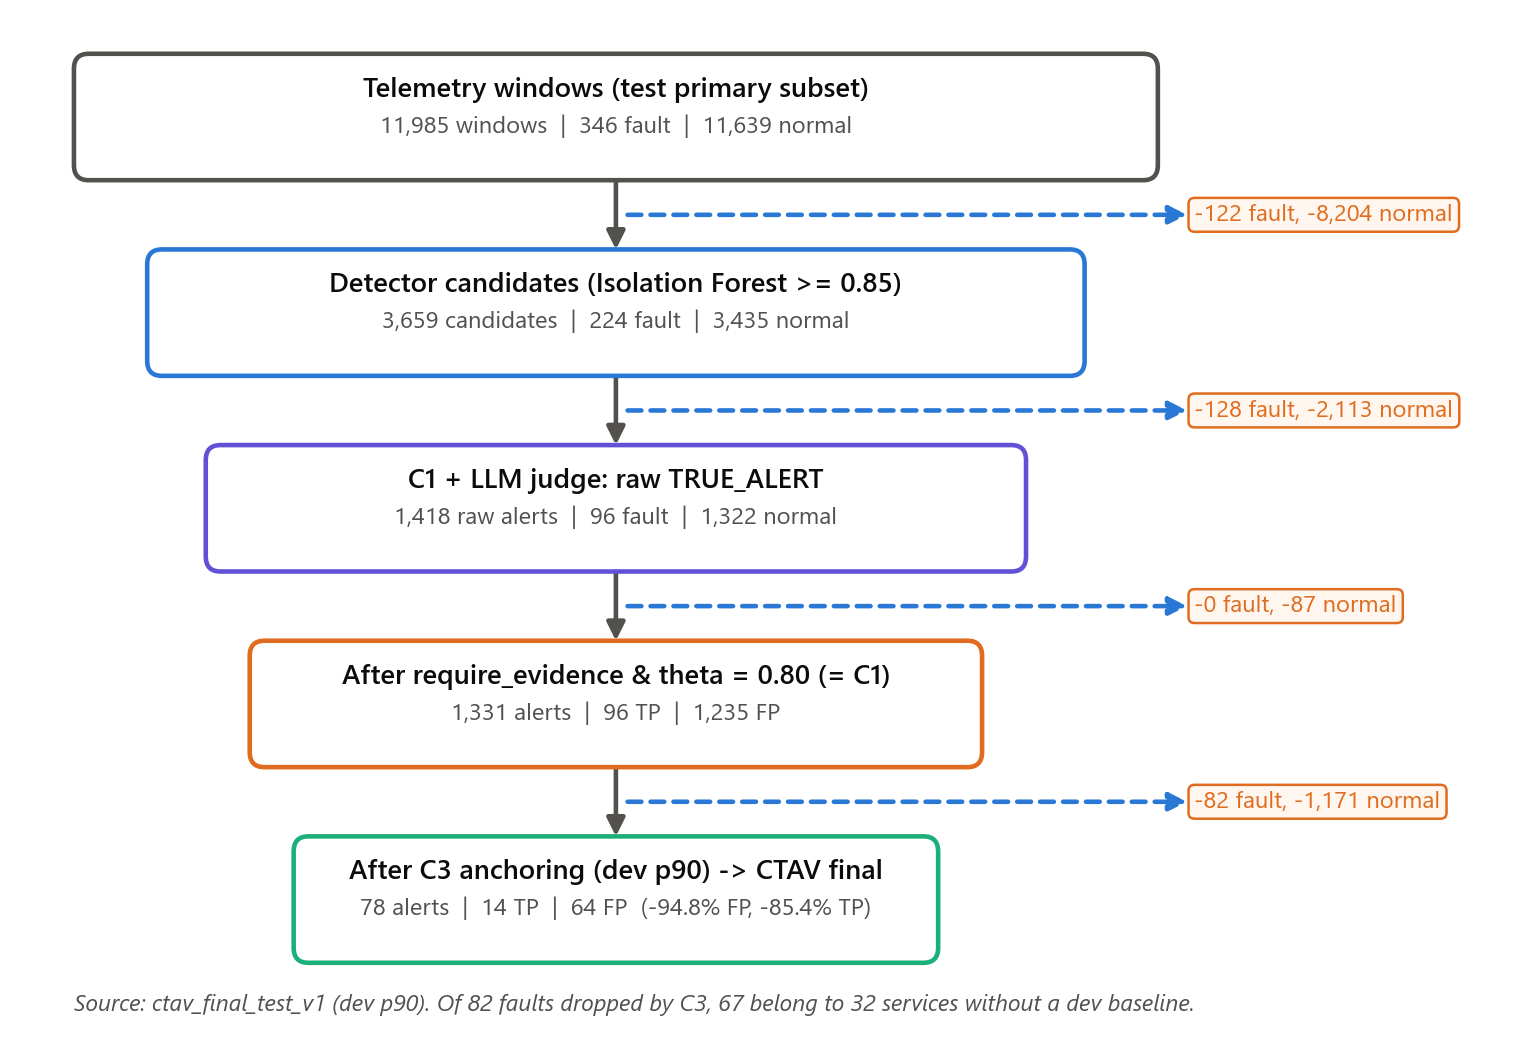
\includegraphics[width=\linewidth]{Images/C1/figures/ch5/h5.11-ctav-funnel-test.png}
  \vspace{0.35cm}
  \caption[Phễu quyết định của CTAV trên tập test]{Phễu quyết định của \CTAV{} trên $11.985$ cửa sổ có telemetry của \splitname{test}, cho thấy tầng C3 cắt $94{,}8\%$ FP nhưng đồng thời hạ $82$ TP (trong đó $67$ TP thuộc các service thiếu ngưỡng \splitname{dev}). \emph{(Nguồn: tác giả vẽ, có hỗ trợ AI.)}}
  \label{fig:ch5-funnel}
\end{figure}

Bảng~\ref{tab:ch5-ablation-both} đối chiếu đầy đủ các biến thể ablation trên \splitname{test} cạnh tham chiếu \splitname{val}. Hai thành phần bị loại (C2, C4) tiếp tục không mang lại lợi ích trên \splitname{test}: mọi phán quyết bị C2 chặn đều đã bị C3 chặn từ trước (McNemar $p = 1{,}000$), còn C4 đẩy tổng số lượt gọi lên $16.985$ (do $10.412$ ca không có ngữ cảnh ở tầng 1 đều leo thang sang tầng 2) mà chỉ phát sinh thêm $4$ FP.

\begin{table}[htbp]
  \centering
  \caption[Bảng ablation thành phần quanh CTAV trên test cạnh val]{Hiệu năng các biến thể ablation quanh \CTAV{} trên \splitname{test} ($11.985$ cửa sổ có telemetry, $346$ lỗi) đối chiếu với \splitname{val}.}
  \label{tab:ch5-ablation-both}
  \scriptsize
  \renewcommand{\arraystretch}{1.15}
  \setlength{\tabcolsep}{2.5pt}
  \begin{tabularx}{\linewidth}{@{}Y r r r c r r r@{}}
    \toprule
    \textbf{Biến thể (\splitname{test})} & \textbf{TP / FP} & \textbf{Prec.} & \textbf{Recall} & \textbf{F1 [CI95]} & \textbf{FPR} & \textbf{USD} & \textbf{\splitname{val} F1} \\
    \midrule
    \textbf{\CTAV{}} (\splitname{dev} $p_{90}$) & 14 / 64 & 0,179 & 0,040 & 0,066 [0,036; 0,100] & 0,0055 & 8,16 & 0,201 \\
    Bỏ C3 (\code{no\_c3} = C1) & 96 / 1.235 & 0,072 & 0,277 & 0,114 [0,093; 0,135] & 0,1061 & 8,16 & 0,126 \\
    + C2 ($\theta_{\text{topo}} = 0{,}85$) & 14 / 64 & 0,179 & 0,040 & 0,066 [0,036; 0,100] & 0,0055 & 8,16 & 0,202 \\
    + C4 (\code{fp\_conf = 0,95}) & 14 / 68 & 0,171 & 0,040 & 0,065 [0,036; 0,099] & 0,0058 & 13,56 & 0,188 \\
    \textbf{C3-trượt} (60 phút $p_{90}$) & \textbf{47 / 391} & \textbf{0,107} & \textbf{0,136} & \textbf{0,120 [0,090; 0,151]} & \textbf{0,0336} & 8,16 & 0,137 \\
    \bottomrule
  \end{tabularx}
\end{table}

\subsubsection{Độ phủ ngưỡng nền \splitname{dev} và sự sụt giảm recall (Phát hiện 11)}
\label{sec:ch5-finding11}

Vì sao C3 (\splitname{dev} $p_{90}$) chỉ làm rơi $26/55$ TP trên \splitname{val} nhưng làm rơi tới $82/96$ TP trên \splitname{test}? Bảng~\ref{tab:ch5-finding11} và Hình~\ref{fig:ch5-finding11} tách toàn bộ cửa sổ có telemetry của hai split thành hai nhóm: service có ít nhất một ngưỡng thao tác hợp lệ trong \code{span\_baseline.parquet} (dựng từ $14$ service có cửa sổ bình thường sạch trong \splitname{dev}) và service không có ngưỡng nào. Do phần lớn service trên Nezha không ghi log \code{ERROR}/\code{WARN} trực tiếp lên pod có cửa sổ metric, mọi cảnh báo trên nhóm service thiếu ngưỡng nền \splitname{dev} đều bị C3 hạ về $0$.

\begin{figure}[htbp]
  \centering
  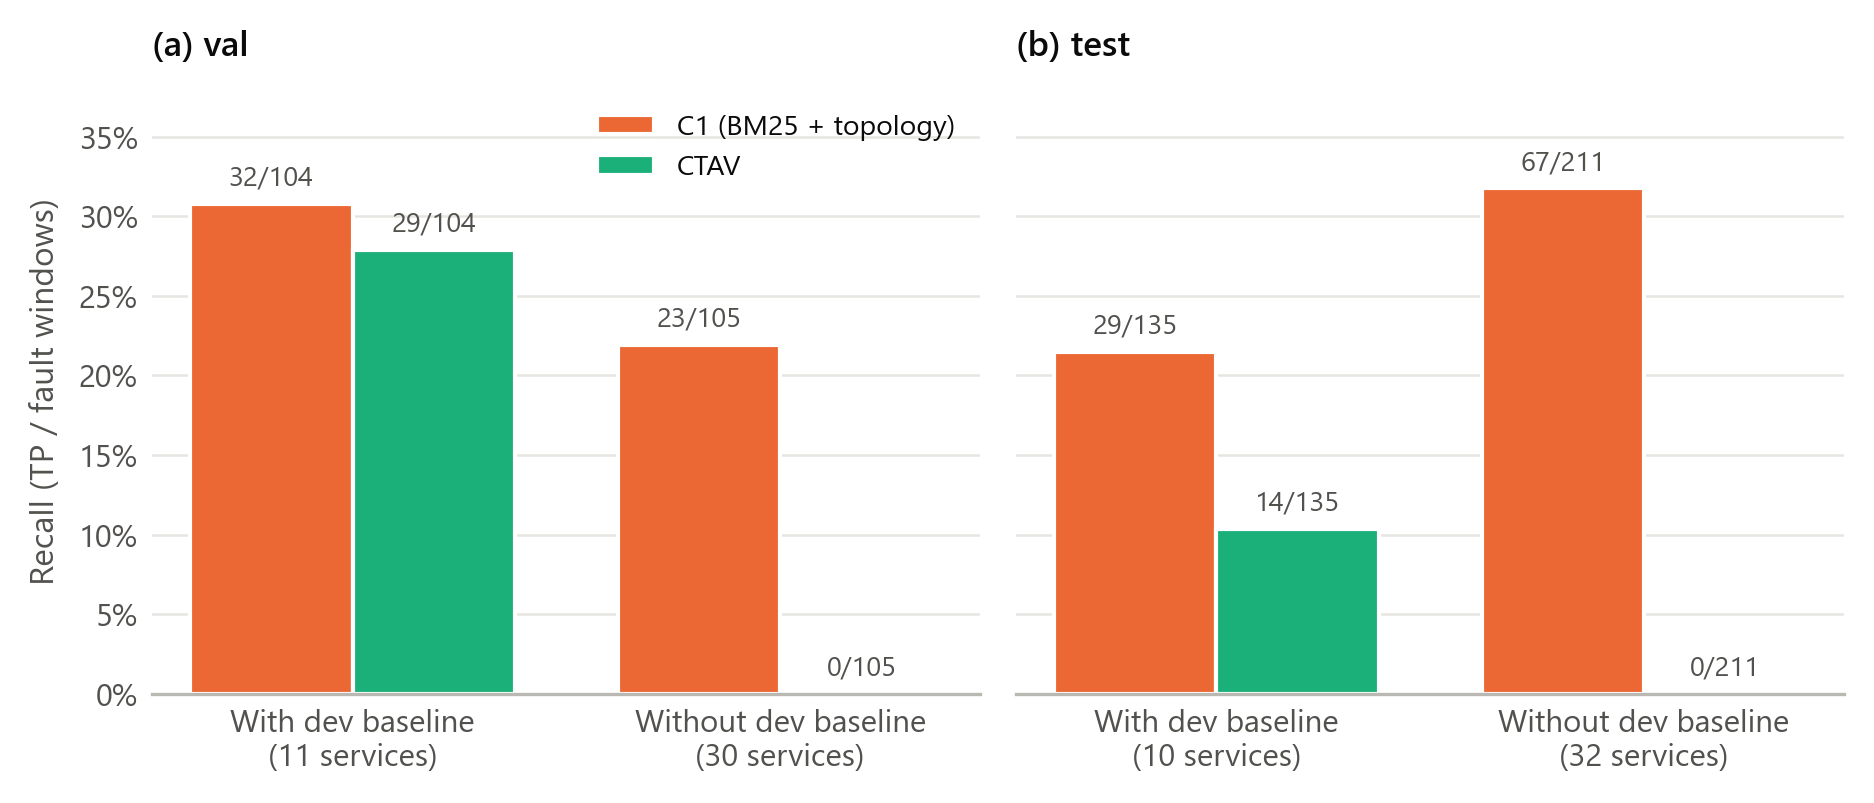
\includegraphics[width=0.92\linewidth]{Images/C1/figures/ch5/h5.12-recall-by-service-group.png}
  \vspace{0.35cm}
  \caption[Recall của C1 và CTAV theo nhóm service có và thiếu ngưỡng dev]{Recall của C1 và \CTAV{} tách theo nhóm service có và không có ngưỡng nền \splitname{dev} trên (a)~\splitname{val} và (b)~\splitname{test}; ở nhóm thiếu ngưỡng, \CTAV{} mất trắng $100\%$ TP.}
  \label{fig:ch5-finding11}
\end{figure}

\begin{table}[htbp]
  \centering
  \caption[Phân tách C1 và CTAV theo độ phủ ngưỡng nền dev của service]{So sánh C1 và \CTAV{} (\splitname{dev} $p_{90}$) theo nhóm service có và không có ngưỡng nền \splitname{dev} trên \splitname{val} và \splitname{test}.}
  \label{tab:ch5-finding11}
  \scriptsize
  \renewcommand{\arraystretch}{1.15}
  \begin{tabularx}{\linewidth}{@{}Y r r r r@{}}
    \toprule
    \textbf{Chỉ tiêu (cửa sổ có telemetry)} & \textbf{\splitname{val}: có \splitname{dev}} & \textbf{\splitname{val}: thiếu} & \textbf{\splitname{test}: có \splitname{dev}} & \textbf{\splitname{test}: thiếu} \\
    \midrule
    Số service có cửa sổ telemetry / có lỗi & 11 / 8 & 30 / 10 & 10 / 9 & 32 / 11 \\
    Cửa sổ có telemetry & 1.438 & 6.198 & 1.428 & 10.557 \\
    Cửa sổ lỗi / lỗi là candidate & 104 / 50 & 105 / 59 & 135 / 93 & 211 / 131 \\
    C1: TP / FP & 32 / 290 & 23 / 316 & 29 / 99 & 67 / 1.136 \\
    \CTAV{} (\splitname{dev} $p_{90}$): TP / FP & 29 / 51 & \textbf{0 / 0} & 14 / 64 & \textbf{0 / 0} \\
    Recall C1 & 0,308 & 0,219 & 0,215 & 0,318 \\
    Recall \CTAV{} (\splitname{dev} $p_{90}$) & 0,279 & \textbf{0,000} & 0,104 & \textbf{0,000} \\
    \bottomrule
  \end{tabularx}
\end{table}

Trên \splitname{test}, có tới $88{,}1\%$ cửa sổ telemetry ($10.557/11.985$) và $61{,}0\%$ cửa sổ lỗi ($211/346$) rơi vào $32$ service thiếu ngưỡng \splitname{dev} — gồm hàng loạt service mang nhiều TP nhất của C1 như \code{checkoutservice} ($17$ TP), \code{currencyservice} ($10$), \code{adservice} ($9$), \code{ts-food-service} ($9$), \code{productcatalogservice} ($8$), \code{ts-preserve-service} ($7$) và \code{ts-basic-service} ($5$). Việc hạ trọn $67/67$ TP trên nhóm này làm \CTAV{} mất ngay $0{,}194$ recall toàn tập. Khi thay duy nhất nguồn ngưỡng bằng cửa sổ trượt 60 phút không cần nhãn (\code{C3-trượt}, nâng độ phủ span C1 từ $16{,}1\%$ lên $91{,}2\%$), hệ thống giữ được $47$ TP (nhiều hơn BM25 $13$ TP, tức $+38\%$), cắt $68{,}3\%$ FP của C1 ($1.235 \to 391$, đưa FPR về $0{,}0336$ sát mức $0{,}0317$ của BM25) và đạt F1 cao nhất toàn bảng ($0{,}120$, vượt \CTAV{} đóng băng có ý nghĩa thống kê với $\Delta\text{F1} = +0{,}054$ $[+0{,}017;\, +0{,}091]$, $p < 0{,}001$). Kết quả này chứng minh \emph{nguyên lý neo bằng chứng C3 đúng}, còn sự thất bại của H2 bắt nguồn từ tính mong manh của ngưỡng tĩnh \splitname{dev} trước độ lệch thành phần service.

\subsubsection{Đường F1 theo ngân sách gọi LLM}
\label{sec:ch5-budget}

Hình~\ref{fig:ch5-budget} và Bảng~\ref{tab:ch5-budget} theo dõi F1 dọc theo các mốc ngân sách $\{120, 250, 500, 1.000, 2.000, 4.000, \text{đủ}\}$ khi duyệt candidate theo thứ tự thời gian. Trên \splitname{test}, \CTAV{} dẫn trước BM25 và LLM-không-RAG ở mốc $120$, nhưng đi ngang quanh $0{,}032$--$0{,}036$ từ mốc $500$ đến $4.000$ rồi mới tăng lên $0{,}066$ ở mức đủ ($13.699$ candidate). Có hai lý do kỹ thuật trực tiếp: (1) giữa mốc $1.001$ và $4.000$, các candidate phát sinh đều rơi vào khoảng chạy nền không có telemetry nên mọi chỉ số không đổi; và (2) toàn bộ $4.000$ candidate đầu tiên nằm trọn trong ngày đầu tiên của OnlineBoutique, nơi phần lớn sự cố sau mốc $120$ thuộc các service thiếu ngưỡng \splitname{dev}, khiến C1 tăng lên $39$ TP ($\text{F1} = 0{,}142$) trong khi \CTAV{} đóng băng dừng ở $7$ TP.

\begin{figure}[htbp]
  \centering
  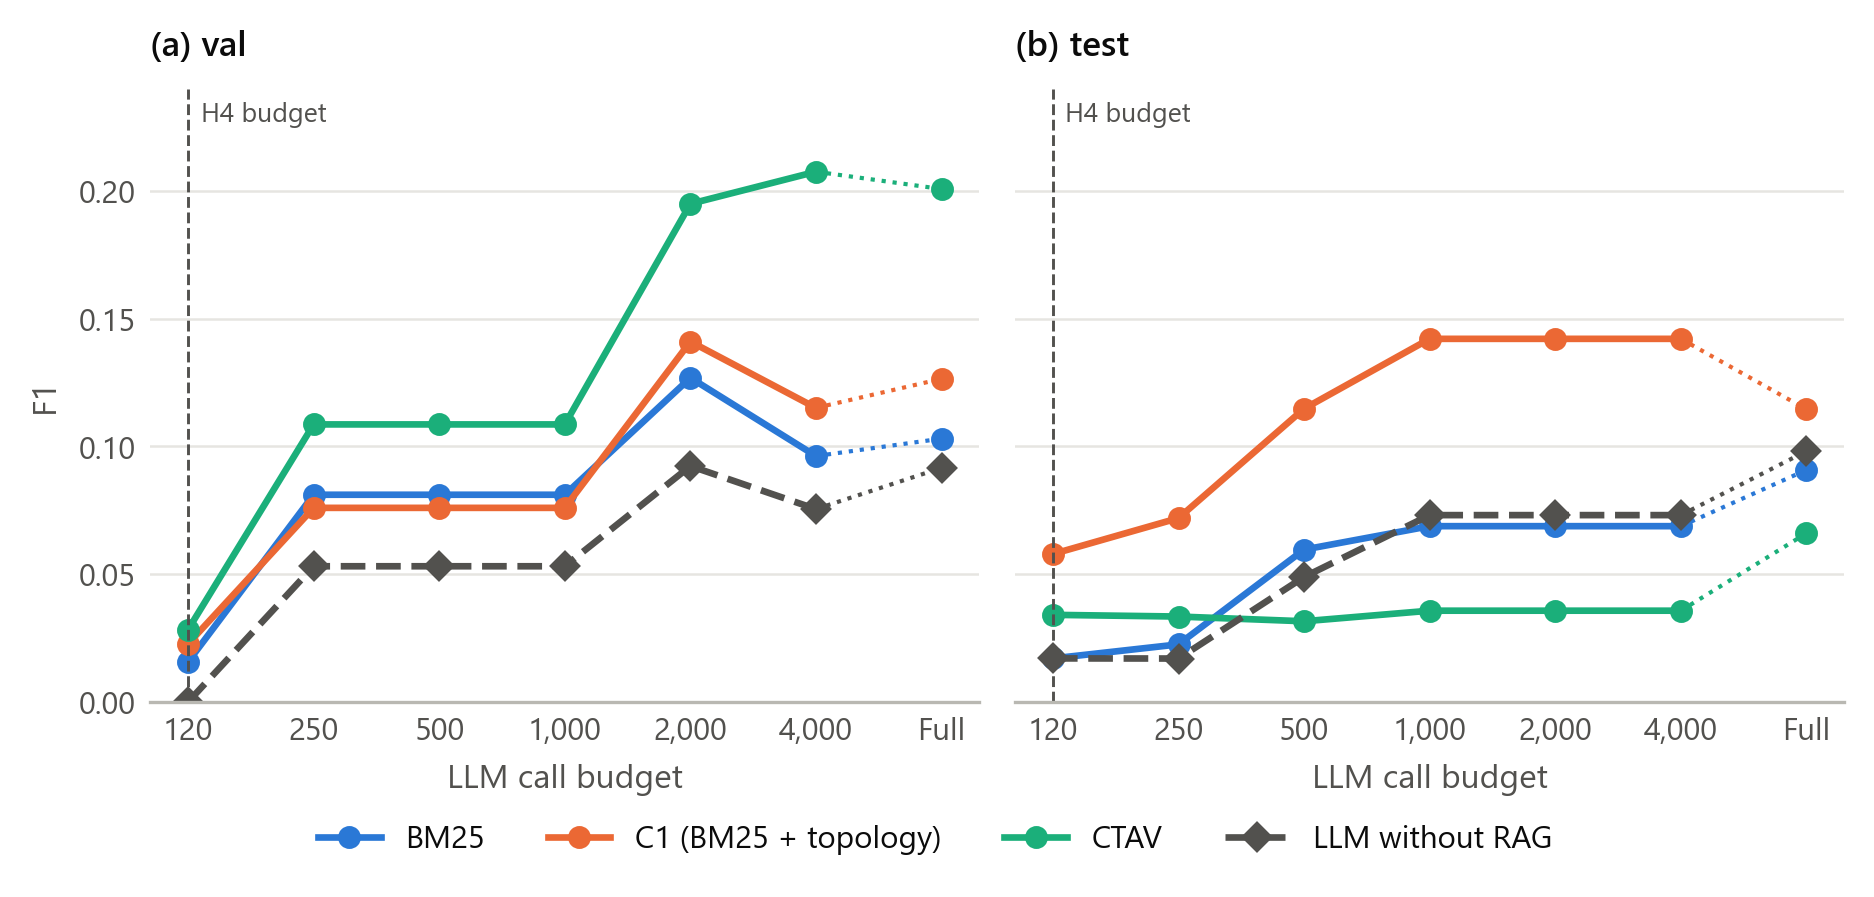
\includegraphics[width=\linewidth]{Images/C1/figures/ch5/h5.13-f1-vs-budget.png}
  \vspace{0.35cm}
  \caption[Đường F1 theo ngân sách lần gọi LLM trên val và test]{Đường cong F1 theo ngân sách lượt gọi LLM (thang log, duyệt theo thứ tự thời gian) trên cửa sổ có telemetry của (a)~\splitname{val} và (b)~\splitname{test}; vạch đứt đánh dấu mốc 120 của H4.}
  \label{fig:ch5-budget}
\end{figure}

\begin{table}[htbp]
  \centering
  \caption[Giá trị F1 theo ngân sách lần gọi LLM trên test]{F1 của bốn phương pháp theo các mốc ngân sách lượt gọi LLM trên \splitname{test} ($11.985$ cửa sổ có telemetry, $346$ lỗi; mức đủ $= 13.699$ candidate).}
  \label{tab:ch5-budget}
  \scriptsize
  \renewcommand{\arraystretch}{1.15}
  \begin{tabularx}{\linewidth}{@{}Y r r r r r r r@{}}
    \toprule
    \textbf{Phương pháp} & \textbf{120} & \textbf{250} & \textbf{500} & \textbf{1.000} & \textbf{2.000} & \textbf{4.000} & \textbf{Đủ (13.699)} \\
    \midrule
    \textbf{\CTAV{}} & 0,034 & 0,033 & 0,032 & 0,036 & 0,036 & 0,036 & 0,066 \\
    BM25 & 0,017 & 0,023 & 0,060 & 0,069 & 0,069 & 0,069 & 0,091 \\
    C1 & 0,058 & 0,072 & 0,115 & 0,142 & 0,142 & 0,142 & 0,114 \\
    LLM-không-RAG & 0,017 & 0,017 & 0,049 & 0,073 & 0,073 & 0,073 & 0,098 \\
    \bottomrule
  \end{tabularx}
\end{table}

\subsubsection{Đánh giá C5 (Rescue) một điểm trên \splitname{test}}
\label{sec:ch5-test-c5}

Giữ nguyên điểm tham số đã chốt trên \splitname{val} ($\eta = (0;\, 0{,}4;\, 0{,}6)$, $\tau = 0{,}8$), cổng Rescue vớt lên $61$ cửa sổ trên \splitname{test} ($3$ lỗi trong $122$ lỗi bị detector bỏ sót và $58$ bình thường; chi phí $0{,}09$ USD). Khi qua C1 và judge, cả $3$ cửa sổ lỗi đều bị judge trả \code{FALSE\_POSITIVE} trước khi tới C3, còn $58$ cửa sổ bình thường phát sinh $1$ FP cuối cùng (Bảng~\ref{tab:ch5-test-c5}; $\Delta\text{F1} = 0{,}000$, McNemar $p = 1{,}000$), xác nhận lại Phát hiện 12 trên dữ liệu độc lập.

\begin{table}[htbp]
  \centering
  \caption[So sánh CTAV và CTAV + C5 một điểm trên val và test]{Ảnh hưởng của cổng cứu cảnh báo C5 tại điểm cố định $\eta = (0;\, 0{,}4;\, 0{,}6)$, $\tau = 0{,}8$ trên cả hai split \splitname{val} và \splitname{test}.}
  \label{tab:ch5-test-c5}
  \scriptsize
  \renewcommand{\arraystretch}{1.15}
  \begin{tabularx}{\linewidth}{@{}Y l r r r r c r@{}}
    \toprule
    \textbf{Biến thể} & \textbf{Split} & \textbf{Cửa sổ cứu} & \textbf{TP} & \textbf{FP} & \textbf{Recall} & \textbf{F1 [CI95]} & \textbf{FPR} \\
    \midrule
    \CTAV{} (tắt C5) & \splitname{val} & 0 & 29 & 51 & 0,139 & 0,201 [0,138; 0,264] & 0,0069 \\
    \CTAV{} + C5 & \splitname{val} & 52 & 31 & 67 & 0,148 & 0,202 [0,143; 0,261] & 0,0090 \\
    \CTAV{} (tắt C5) & \splitname{test} & 0 & 14 & 64 & 0,040 & 0,066 [0,036; 0,100] & 0,0055 \\
    \CTAV{} + C5 & \splitname{test} & 61 & 14 & 65 & 0,040 & 0,066 [0,036; 0,101] & 0,0056 \\
    \bottomrule
  \end{tabularx}
\end{table}

\subsubsection{Độ ổn định lặp lại của bộ thẩm định và đối chiếu chi phí}
\label{sec:ch5-repeat}

Để đo nhiễu nội tại của \code{gemini-2.5-flash} tại nhiệt độ $0$, hai nhánh BM25 và C1 được gọi lặp độc lập thêm hai lần (\code{repeat} $= 1, 2$) trên cùng mẫu ngẫu nhiên $200$ candidate có telemetry của \splitname{test} ($6$ lỗi, $194$ bình thường, \code{seed = 42}). Bảng~\ref{tab:ch5-repeat} cho thấy độ đồng thuận $3/3$ lần đạt $99{,}0\%$ ở BM25 ($2/200$ cửa sổ bình thường đổi nhãn) và $99{,}5\%$ ở C1 ($1/200$ cửa sổ bình thường đổi nhãn); $0$ cửa sổ lỗi bị lật quyết định ở cả hai nhánh. Biên độ nhiễu $0{,}005$--$0{,}010$ nhỏ hơn một bậc độ lớn so với các hiệu ứng chính ($\Delta\text{Recall} = +0{,}179$, $\Delta\text{FPR} = -0{,}0262$), xác nhận kết luận kiểm định ổn định trước phương sai API. Tổng chi phí G-test đạt $15{,}85$ USD ($23{,}37$ triệu token vào, $3{,}53$ triệu token ra) so với ước tính ban đầu $13{,}00$ USD (vượt $2{,}85$ USD chủ yếu do tỷ lệ prompt có bằng chứng và độ dài chuỗi span của OnlineBoutique trên \splitname{test} lớn hơn \splitname{val}).

\begin{table}[htbp]
  \centering
  \caption[Độ ổn định phán quyết của judge qua ba lần gọi độc lập]{Độ lệch câu trả lời của \code{gemini-2.5-flash} qua \code{repeat} $= 0, 1, 2$ trên mẫu 200 candidate có telemetry của \splitname{test} ($6$ lỗi, $194$ bình thường).}
  \label{tab:ch5-repeat}
  \scriptsize
  \renewcommand{\arraystretch}{1.15}
  \begin{tabularx}{\linewidth}{@{}l r c c Y@{}}
    \toprule
    \textbf{Phương pháp} & \textbf{Mẫu} & \textbf{\code{TRUE\_ALERT} thô (r0 / r1 / r2)} & \textbf{Cảnh báo cuối (r0 / r1 / r2)} & \textbf{Tỷ lệ lật nhãn [CI95]} \\
    \midrule
    BM25 & 200 & 0,120 / 0,110 / 0,120 (24/22/24) & 0,085 / 0,075 / 0,085 (17/15/17) & 0,010 [0,000; 0,025] (2/200) \\
    C1 & 200 & 0,370 / 0,375 / 0,375 (74/75/75) & 0,335 / 0,340 / 0,340 (67/68/68) & 0,005 [0,000; 0,015] (1/200) \\
    \bottomrule
  \end{tabularx}
\end{table}

\subsubsection{Đánh giá context precision bằng chấm tay}
\label{sec:ch5-context-precision}

Để đánh giá chất lượng bằng chứng truy xuất độc lập với bộ thẩm định LLM, hệ thống đã trích xuất ngẫu nhiên một mẫu mù gồm $50$ cửa sổ có telemetry trên \splitname{test} ($25$ lỗi, $25$ bình thường, \code{seed = 42}) thành $525$ dòng bằng chứng phân biệt tại \code{eval/manual/context\_precision\_test\_v1.csv}, tách hoàn toàn nhãn phương pháp (BM25 hay C1) và nhãn cửa sổ sang tệp khóa riêng. Quy trình chấm theo thang ba mức (\code{relevant}, \code{irrelevant}, \code{unsure}) sẽ bổ sung số liệu hoàn chỉnh vào Bảng~\ref{tab:ch5-ctx-prec} sau khi hoàn tất phiên chấm tay.

\begin{table}[htbp]
  \centering
  \caption[Khung bảng đánh giá context precision chấm tay trên mẫu 50 cửa sổ test]{Khung tổng hợp \emph{context precision} chấm tay trên mẫu mù 50 cửa sổ có telemetry của \splitname{test} (25 lỗi, 25 bình thường; 525 dòng bằng chứng).}
  \label{tab:ch5-ctx-prec}
  \scriptsize
  \renewcommand{\arraystretch}{1.15}
  \begin{tabularx}{\linewidth}{@{}l Y c c c c@{}}
    \toprule
    \textbf{Phương pháp} & \textbf{Nhóm cửa sổ} & \textbf{Số bằng chứng} & \textbf{Liên quan} & \textbf{Không liên quan} & \textbf{Context precision} \\
    \midrule
    BM25 & Lỗi (25) / Bình thường (25) & \multicolumn{4}{c}{\CHO{chấm tay}{525 dòng trong \code{context\_precision\_test\_v1.csv}}} \\
    C1 & Lỗi (25) / Bình thường (25) & \multicolumn{4}{c}{\CHO{chấm tay}{525 dòng trong \code{context\_precision\_test\_v1.csv}}} \\
    \bottomrule
  \end{tabularx}
\end{table}

% -----------------------------------------------------------------------------
\subsection{Đánh giá tác tử RCA (H5)}
\label{sec:ch5-rca}

Mục này trình bày kết quả lựa chọn tham số tác tử RCA trên \splitname{val} và kiểm định chính thức giả thuyết H5 trên tập \splitname{test}.

\subsubsection{Chọn tham số trên \splitname{val} và thiết lập kiểm định H5}
\label{sec:ch5-rca-setup}

Trên $80$ cảnh báo của \CTAV{} trên \splitname{val}, hệ thống quét $T_{\text{group}} \in \{180, 300, 600\}\,\text{s}$ theo quy tắc định trước (ưu tiên tối thiểu số sự cố đa lỗi nhập nhằng \code{ambiguous} rồi đến ARR). Mức $T_{\text{group}} = 180\,\text{s}$ được chọn vì tạo $1$ sự cố \code{ambiguous} so với $2$ sự cố ở $300\,\text{s}$ và $600\,\text{s}$ (ARR mọi cảnh báo đạt $0{,}675$; Hit@1 mức 1 bằng baseline $= 7/11 = 0{,}636$; JSON valid rate $26/26 = 1{,}000$; riêng ARR trên \code{network\_delay} chỉ đạt $0{,}250$ do thiếu cảnh báo đầu vào). Cấu hình chốt (\code{eval/configs/rca\_final.yaml}, dấu vân tay \code{b0c54fa68ef65535}) được sao nguyên sang \splitname{test} để chạy một lần lên đúng $78$ cảnh báo của \CTAV{} đóng băng. Ngoài kết quả đăng ký chính thức, một dòng \emph{độ nhạy ngoài bản đăng ký} được chạy trên $438$ cảnh báo của \code{c3\_rolling\_baseline} để tách ảnh hưởng của độ phủ cảnh báo đầu vào khỏi bản thân thuật toán định vị; dòng độ nhạy chỉ mang tính phân tích và không dùng thay đổi kết luận H5.

\subsubsection{Kết quả kiểm định H5 trên \splitname{test}}
\label{sec:ch5-rca-results}

Bảng~\ref{tab:ch5-h5} đối chiếu bốn vế đã đăng ký của H5 trên \splitname{test} ($78$ cảnh báo $\to$ $38$ sự cố, gồm $17$ sự cố có nhãn đơn lỗi, $3$ sự cố \code{ambiguous} và $18$ sự cố không ứng với lỗi nào). Bảng~\ref{tab:ch5-rca-compare} đặt song song ba lượt chạy (\splitname{val}, \splitname{test} đăng ký và \splitname{test} độ nhạy), còn Bảng~\ref{tab:ch5-rca-by-fault} phân rã kết quả theo năm loại lỗi tiêm.

\begin{table}[htbp]
  \centering
  \caption[Kiểm định giả thuyết H5 trên tập test theo bản đăng ký]{Kết quả kiểm định H5 trên tập \splitname{test} theo cấu hình đăng ký ($78$ cảnh báo \CTAV{} $\to$ $38$ sự cố, $17$ sự cố có nhãn).}
  \label{tab:ch5-h5}
  \scriptsize
  \renewcommand{\arraystretch}{1.15}
  \begin{tabularx}{\linewidth}{@{}Y >{\raggedright\arraybackslash}p{4.4cm} c l@{}}
    \toprule
    \textbf{Vế tiêu chí H5} & \textbf{Số đo trên \splitname{test}} & \textbf{CI95} & \textbf{Kết quả} \\
    \midrule
    $\text{Hit@1} \ge 0{,}60$ & $8 / 17 = 0{,}471$ & $[0{,}235;\, 0{,}706]$ & \textbf{Không đạt} \\
    $\text{Hit@3} \ge 0{,}80$ & $8 / 17 = 0{,}471$ & $[0{,}235;\, 0{,}706]$ & \textbf{Không đạt} \\
    Cận dưới CI95 $\Delta\text{Hit@1}(\text{RCA}-\text{baseline}) > 0$ & $0{,}000$ (baseline $8/17$; $0$ cặp lệch) & $[0{,}000;\, 0{,}000]$ & \textbf{Không đạt} \\
    Alert Reduction $\ge 30\%$ trên cascade & Không tính được ($0/50$ lần tiêm là cascade) & -- & \textbf{Không đạt} \\
    \bottomrule
  \end{tabularx}
\end{table}

\textbf{H5 không được chấp nhận trên tập \splitname{test} (0/4 vế đạt).} Để tham chiếu, tỷ lệ giảm cảnh báo chung (ARR mọi cảnh báo) đạt $0{,}513$ $[0{,}362;\, 0{,}626]$ và trên cảnh báo trong khoảng lỗi đạt $0{,}556$ $[0{,}382;\, 0{,}674]$, nhưng hai chỉ số này không phải tiêu chí cascade đã đăng ký.

\begin{table}[htbp]
  \centering
  \caption[So sánh tác tử RCA trên val, test đăng ký và dòng độ nhạy]{Đối chiếu tác tử RCA trên \splitname{val}, \splitname{test} đăng ký (\CTAV{} \splitname{dev} $p_{90}$) và dòng độ nhạy ngoài đăng ký (\code{c3\_rolling\_baseline}).}
  \label{tab:ch5-rca-compare}
  \scriptsize
  \renewcommand{\arraystretch}{1.15}
  \setlength{\tabcolsep}{3pt}
  \begin{tabularx}{\linewidth}{@{}Y >{\raggedright\arraybackslash}p{2.9cm} >{\raggedright\arraybackslash}p{3.0cm} >{\raggedright\arraybackslash}p{3.1cm}@{}}
    \toprule
    \textbf{Chỉ số} & \textbf{\splitname{val}} & \textbf{\splitname{test} (đăng ký)} & \textbf{\splitname{test} (độ nhạy, ngoài ĐK)} \\
    \midrule
    Cảnh báo vào / số service & 80 / 8 & 78 / 5 & 438 / 22 \\
    Lần tiêm: tổng / có nhãn / 0 cảnh báo & 30 / 10 / 18 & 50 / 17 / \textbf{29} & 50 / 34 / 1 \\
    Sự cố: tổng / có nhãn / mơ hồ / không lỗi & 26 / 11 / 1 / 14 & 38 / 17 / 3 / 18 & 114 / 48 / 14 / 52 \\
    Sự cố nhiều service & 1 & \textbf{0} & 39 \\
    Hit@1 mức 1 & 0,636 [0,364; 0,909] & \textbf{0,471 [0,235; 0,706]} & 0,208 [0,104; 0,333] \\
    Hit@3 mức 1 & 0,636 [0,364; 0,909] & \textbf{0,471 [0,235; 0,706]} & 0,313 [0,188; 0,458] \\
    Hit@1 baseline / $\Delta\text{Hit@1}$ & 0,636 / 0,000 & 0,471 / \textbf{0,000} & 0,229 / $-0{,}021$ \\
    Hit@1 trên mọi lần tiêm lỗi & 0,200 [0,067; 0,333] & 0,160 [0,060; 0,280] & 0,200 [0,100; 0,320] \\
    ARR mọi cảnh báo & 0,675 [0,600; 0,730] & 0,513 [0,362; 0,626] & 0,740 [0,654; 0,796] \\
    ARR cascade (số lần tiêm cascade) & 0,667 (1) & -- (0) & 0,704 [0,591; 0,777] (41) \\
    JSON valid rate & 26 / 26 (1,000) & \textbf{38 / 38 (1,000)} & 114 / 114 (1,000) \\
    \bottomrule
  \end{tabularx}
\end{table}

\begin{table}[htbp]
  \centering
  \caption[Phân rã kết quả định vị RCA theo loại lỗi trên tập test]{Kết quả định vị service gốc theo năm loại lỗi tiêm trên tập \splitname{test} đăng ký ($50$ lần tiêm lỗi).}
  \label{tab:ch5-rca-by-fault}
  \scriptsize
  \renewcommand{\arraystretch}{1.15}
  \begin{tabularx}{\linewidth}{@{}Y r r r r r@{}}
    \toprule
    \textbf{Loại lỗi tiêm} & \textbf{Lần tiêm} & \textbf{0 cảnh báo} & \textbf{Chỉ ở mơ hồ} & \textbf{Sự cố có nhãn} & \textbf{Trúng hạng 1} \\
    \midrule
    \code{network\_delay} & 15 & 5 & 2 & 8 & 2 \\
    \code{cpu\_contention} & 11 & 5 & 1 & 5 & 3 \\
    \code{exception} & 10 & 7 & 0 & 3 & 3 \\
    \code{return} & 9 & 8 & 0 & 1 & 0 \\
    \code{cpu\_consumed} & 5 & 4 & 1 & 0 & -- \\
    \midrule
    \textbf{Tổng cộng} & \textbf{50} & \textbf{29} & \textbf{4} & \textbf{17} & \textbf{8} \\
    \bottomrule
  \end{tabularx}
\end{table}

\subsubsection{Phân tích nguyên nhân và chất lượng báo cáo JSON}
\label{sec:ch5-rca-analysis}

Cả bốn vế không đạt của H5 quy về cùng một nguyên nhân cấu trúc: \emph{cảnh báo đầu vào hiếm khi rơi đúng vào service gốc}. Trên tập đăng ký, $78$ cảnh báo chỉ phân bố trên $5$ service có ngưỡng nền \splitname{dev} (Phát hiện 11), khiến $29/50$ lần tiêm lỗi không có bất kỳ cảnh báo nào để định vị và toàn bộ $38$ sự cố đều là sự cố một service. Khi một sự cố chỉ chứa một service, thuật toán lan truyền ngược 1 bước trùng tuyệt đối với baseline ($\Delta\text{Hit@1} = 0$, $\text{Hit@3} = \text{Hit@1}$) và không có lỗi cascade để đo ARR. Chín sự cố trượt đều cùng một mẫu: cảnh báo phát ra ở service gọi phía trước (\code{frontend} hoặc \code{ts-travel-service}), còn lỗi tiêm nằm ở service phía sau không phát cảnh báo.

Dòng độ nhạy ($438$ cảnh báo trên $22$ service, $39$ sự cố nhiều service) cho thấy nguyên nhân này không tự mất đi khi tăng số lượng cảnh báo: dù ARR trên $41$ lỗi cascade đạt $0{,}704$ $[0{,}591;\, 0{,}777]$, trong $48$ sự cố có nhãn chỉ có đúng $15$ sự cố chứa service gốc thật trong tập service phát cảnh báo — đặt trần tuyệt đối $15/48 = 0{,}313$ cho mọi thuật toán xếp hạng chỉ nhìn trên tập service đã cảnh báo ($\text{Hit@1} = 0{,}208$, thấp hơn baseline $0{,}021$). Về tầng sinh báo cáo, bộ kiểm duyệt năm quy tắc đạt tỷ lệ JSON hợp lệ $100\%$ ở mọi lượt chạy ($26/26$ trên \splitname{val}, $38/38$ trên \splitname{test} đăng ký, $114/114$ ở độ nhạy; lọc sạch các định danh bằng chứng bịa đặt trong $1$ và $4$ báo cáo), song trường phân loại \code{fault\_type} thiên mạnh về \code{cpu\_contention} ($35/38$ báo cáo) — vấn đề chất lượng nội dung này sẽ được phân tích sâu cùng đánh giá mù bởi con người ở Chương~\ref{ch:thao-luan}.

% -----------------------------------------------------------------------------
\subsection{Tổng hợp mười hai phát hiện thực nghiệm}
\label{sec:ch5-synthesis}

Xuyên suốt quá trình kiểm chứng từ cổng tái lập đến tập \splitname{test} độc lập, đề tài ghi nhận mười hai phát hiện thực nghiệm nối kết trực tiếp lý thuyết với các quyết định thiết kế và giới hạn hệ thống, hệ thống hóa ở Bảng~\ref{tab:ch5-findings}. Bốn nhóm bài học cốt lõi nổi lên rõ rệt: (1) giao thức dữ liệu quyết định mạnh biên độ chỉ số tuyệt đối (Phát hiện 1--4); (2) bộ thẩm định LLM nhạy cảm với các tín hiệu định dạng như cột metric hằng lỗi và với bằng chứng trace sát $t_0$ bất kể nhãn (Phát hiện 5--7); (3) neo bằng chứng C3 là thành phần duy nhất kìm hiệu quả báo động giả, trong khi C2, C4, C5 không đóng góp (Phát hiện 9, 12); và (4) cách ước lượng ngưỡng nền tĩnh từ một split nhỏ (\splitname{dev}) là nút thắt quyết định khiến cấu hình đóng băng đánh mất recall trên \splitname{test}, qua đó kéo theo việc tác tử RCA thiếu cảnh báo ở service gốc (Phát hiện 8, 10, 11).

\begin{table}[htbp]
  \centering
  \caption[Tổng hợp 12 phát hiện thực nghiệm và vai trò trong đề tài]{Tổng hợp 12 phát hiện thực nghiệm xuyên suốt quá trình đánh giá và tác động thiết kế tương ứng.}
  \label{tab:ch5-findings}
  \scriptsize
  \renewcommand{\arraystretch}{1.15}
  \setlength{\tabcolsep}{3.5pt}
  \begin{tabularx}{\linewidth}{@{}r Y >{\raggedright\arraybackslash}p{4.2cm}@{}}
    \toprule
    \textbf{\#} & \textbf{Phát hiện thực nghiệm} & \textbf{Tác động thiết kế / đánh giá} \\
    \midrule
    1 & Trên Nezha, có bằng chứng gần như tương đương với gần sự cố ($100\%$ lỗi so với $\approx 25\%$ bình thường có telemetry) & Chốt tập chấm chính trên cửa sổ có telemetry (Mục~\ref{sec:ch5-data}) \\
    2 & Độ tin cậy của judge khi thiếu ngữ cảnh chủ yếu sao chép lại \code{anomaly\_score} & Không dùng \code{confidence} thô làm tín hiệu hiệu chỉnh duy nhất \\
    3 & Biến thể ``topology'' trên tập mẫu cũ gần giống BM25 không giới hạn thời gian & Giới hạn kho tìm kiếm trong biên $\pm 8$ phút (\code{bm25\_pool = window}) \\
    4 & Công thức C1 chuẩn không tự đưa bằng chứng lân cận vào top-6 khi không có hạn ngạch & Tách khảo sát C1-quota và H0 trên \splitname{val} \\
    5 & Cột \code{PodSuccessRate(\%)} luôn bằng $0$ khiến judge không bác bỏ cảnh báo & Thêm tham số \code{drop\_metrics} loại cột hằng lỗi (Mục~\ref{sec:ch4-judge}) \\
    6 & Thay đổi trọng số Fusion $(\alpha, \beta, \gamma)$ không điều khiển tỷ lệ bằng chứng lân cận & Giữ bộ trọng số chuẩn $(0{,}35;\, 0{,}25;\, 0{,}40)$ và $k_{\text{graph}} = 0$ \\
    7 & H0 tái lập hiện tượng tăng Recall \& FPR nhưng nguyên nhân là trace cục bộ sát $t_0$, không phải nhiễu lân cận & Định hình lại H1 và chuyển trục chính sách sang neo bằng chứng tại $s_0$ \\
    8 & Ngưỡng nền \splitname{dev} $p_{90}$ chỉ phủ $31{,}8\%$--$33{,}2\%$ span trên \splitname{val} ($16{,}1\%$ trên \splitname{test}) & Đưa biến thể \code{C3-trượt} 60 phút vào H3 để đối chứng \\
    9 & Tầng 1 BM25 sinh nhiều FP và tỷ lệ leo thang lớn khiến C4 tốn chi phí hơn C1 chạy thẳng & Loại C4 khỏi cấu hình \CTAV{} chốt (xác nhận lại trên \splitname{test}) \\
    10 & \CTAV{} cắt $91{,}6\%$--$94{,}8\%$ FP nhưng không giữ được recall của C1 & Báo cáo trung thực kết luận H2, không nới tiêu chí đăng ký \\
    11 & Ngưỡng \splitname{dev} gây ``im lặng có cấu trúc'' trên $32/42$ service của \splitname{test} (mất $67/96$ TP của C1) & Giải thích trực tiếp kết quả H2, H5 và khẳng định ưu thế của \code{C3-trượt} \\
    12 & Cổng cứu C5 chỉ thêm $\le 2$ TP trên \splitname{val} và $+0$ TP / $+1$ FP trên \splitname{test} (nút thắt ở judge) & Giữ C5 làm kết quả ablation âm, không bật trong pipeline chính \\
    \bottomrule
  \end{tabularx}
\end{table}

% -----------------------------------------------------------------------------
\subsection{Kết chương}
\label{sec:ch5-ket-chuong}

Chương này đã hoàn tất kiểm định định lượng toàn bộ hệ thống trên ba lớp bằng chứng độc lập: vượt qua hai cổng kỹ thuật G-port và G-paper ($100\%$ cache hit), tinh chỉnh và đóng băng cấu hình trên \splitname{val}, rồi kiểm định một lần duy nhất trên tập \splitname{test} niêm phong. Theo đúng tiêu chí đã đăng ký trước: \textbf{H0 được chấp nhận} (4/4 vế, xác nhận đánh đổi Recall--FPR của C1); \textbf{H1 được giữ một phần} trên \splitname{val} (chỉ ra độ nhạy chung với trace cục bộ sát $t_0$); \textbf{H2 không được chấp nhận} trên \splitname{test} (đạt sâu vế giảm FPR $5{,}8$ lần so với BM25 nhưng mất recall do $32/42$ service thiếu ngưỡng nền \splitname{dev}, trong khi đối chứng \code{C3-trượt} 60 phút nâng F1 lên $0{,}120$); \textbf{H3 được chấp nhận} (khẳng định C3 là đóng góp lõi và xác nhận loại C2, C4, giữ C5 làm ablation âm); \textbf{H4 được chấp nhận} ở mốc $120$ lượt gọi; và \textbf{H5 không được chấp nhận} (0/4 vế do cảnh báo đầu vào thưa và hiếm rơi vào service gốc, dù JSON valid rate đạt $100\%$ và ARR cascade ở dòng độ nhạy đạt $0{,}704$). Các kết quả và công cụ kiểm chứng này được tích hợp trực tiếp vào nền tảng trình diễn ở Chương~\ref{ch:platform} và phân tích sâu nguyên nhân ca sai ở Chương~\ref{ch:thao-luan}.

 \newpage
 % =============================================================================
% Chuong 6: Platform demo (chuan lop article cho Internship2_HK262)
% Nguon noi dung: docs/drafts/ch6-demo-platform.md, outline-bao-cao-gd2.md (Ch6),
%   eval/results/{pipeline_val_v2,pipeline_test_v2,pipeline_sens_test_v1}/runtime.json,
%   eval/results/m10_demo_cases_v1/demo_cases.json, docs/milestones/M11-danh-gia-nguoi.md
% Nhan dung tu chuong khac: ch:de-xuat, ch:thuc-nghiem, ch:thao-luan,
%   sec:ch4-c1, sec:ch4-policy, sec:ch4-rca, sec:ch4-grouping, sec:ch4-propagation,
%   sec:ch4-report, sec:ch4-impl, sec:ch2-cong-nghe, sec:ch5-rca-results,
%   sec:ch5-finding11, tab:ch5-findings, tab:ch5-verdict-summary
% =============================================================================

\section{Platform demo}
\label{ch:platform}

Chương này trả lời câu hỏi liệu toàn bộ chuỗi xử lý ở Chương~\ref{ch:de-xuat}, từ bộ phát hiện bất thường qua \CTAV{} tới tác tử \term{RCA}{RCA}, có vận hành được thành một hệ thống điều hành trực quan mà kỹ sư trực ca và hội đồng thẩm định dùng được hay không. Chương không đưa ra kết quả thực nghiệm mới; mọi con số đều đọc lại từ các lượt chạy đã đóng băng ở Chương~\ref{ch:thuc-nghiem}. Mục~\ref{sec:ch6-vai-tro} xác định vai trò, phạm vi và cơ chế tách lớp hiển thị của platform. Mục~\ref{sec:ch6-luong} mô tả luồng dữ liệu đầu--cuối, tám endpoint chỉ đọc và kiến trúc triển khai bằng Docker Compose. Mục~\ref{sec:ch6-dashboard} đi qua năm màn hình theo trình tự thao tác thực tế, Mục~\ref{sec:ch6-kich-ban} trình bày kịch bản demo năm phút, và Mục~\ref{sec:ch6-kiem-thu} báo cáo kết quả kiểm thử ngoại tuyến cùng phương án dự phòng không phụ thuộc Docker.

% -----------------------------------------------------------------------------
\subsection{Vai trò của platform}
\label{sec:ch6-vai-tro}

Mục này làm rõ platform được xây để chứng minh điều gì và chủ đích giới hạn ở đâu. Platform là hiện thực chạy được của \CTAV{} và tác tử \term{RCA}{RCA}: cùng một pipeline vừa xuất các tệp kiểm định \hyp{H0}--\hyp{H5}, vừa nạp dữ liệu cho giao diện điều hành. Nhờ vậy, bất kỳ cảnh báo, sự cố hay nút đồ thị nào hiển thị trên màn hình cũng đối ứng một--một với bản ghi trong kho kết quả của Chương~\ref{ch:thuc-nghiem}, không tồn tại dữ liệu mô phỏng riêng cho trình diễn. Giao diện tách bạch hai chế độ quan sát qua công tắc trên thanh công cụ: chế độ vận hành (\emph{Ops View}) ẩn hoàn toàn nhãn lỗi chuẩn để phản ánh đúng thông tin mà người trực ca nhìn thấy, trong khi lớp phủ đánh giá (\emph{Eval Overlay}) bật đường lỗi chuẩn Nezha và huy hiệu đối chiếu đúng/sai phục vụ hội đồng kiểm chứng. Vì mục tiêu ưu tiên tính tái lập khoa học thay vì vận hành thương mại, hệ thống không cài đặt xác thực người dùng, không phân quyền đa thuê bao, không bắn thông báo ra ngoài và không tự động thực thi kịch bản khắc phục.

Ràng buộc thiết kế thứ hai là toàn bộ buổi trình diễn phải vận hành độc lập khi ngắt hoàn toàn Internet. Mọi phán quyết của judge \code{gemini-2.5-flash} và mọi báo cáo chẩn đoán đều đọc lại từ bộ nhớ đệm (\code{cache}) trên đĩa theo khóa băm ở Mục~\ref{sec:ch4-judge}. Khi bật cờ \code{DEMO\_OFFLINE=1}, pipeline xóa ngay các biến khóa API khỏi tiến trình sau bước nạp cấu hình; nếu phát sinh dù chỉ một truy vấn hụt cache, tiến trình lập tức báo lỗi dừng thay vì âm thầm gọi mạng. Ứng dụng web cũng đóng gói cục bộ toàn bộ biểu tượng vector, bảng màu và mã nguồn, không tải phông chữ hay thư viện từ máy chủ bên ngoài.

% -----------------------------------------------------------------------------
\subsection{Luồng end-to-end và triển khai}
\label{sec:ch6-luong}

Mục này trình bày đường đi của dữ liệu từ tệp quan sát tới giao diện người dùng và cách bố trí các thành phần trên máy trình diễn. Luồng xử lý tuân thủ đúng thứ tự kiến trúc ở Hình~\ref{fig:ch4-arch}. Bộ phát lại đưa từng cửa sổ \code{metric} 60 giây vào bộ phát hiện \term{IF}{Isolation Forest}; các \code{candidate} vượt ngưỡng $0{,}85$ đi qua \CTAV{} gồm \comp{C1} (truy xuất lai \term{BM25}{BM25}--topology), judge \term{LLM}{LLM} đọc từ cache và chính sách quyết định có \comp{C3} (neo bằng chứng theo ngưỡng nền $p_{90}$ của \splitname{dev}). Hai thành phần \comp{C2} (ngưỡng bất đối xứng theo nguồn bằng chứng) và \comp{C4} (định tuyến hai tầng thích nghi) đã bị loại sau kiểm định trên \splitname{val}, còn \comp{C5} (\term{RescueScore}{Rescue Score}) chỉ dùng cho phân tích ablation, nên cả ba không kích hoạt trên luồng chính. Các cảnh báo giữ nhãn \code{TRUE\_ALERT} tiếp tục đi sang tác tử \term{RCA}{RCA} để gom cụm trong cửa sổ $T_{\text{group}} = 180\,\text{s}$, bỏ phiếu lan truyền ngược một bước trên đồ thị gọi và sinh báo cáo JSON có kiểm duyệt (Mục~\ref{sec:ch4-rca}).

Hình~\ref{fig:ch6-deploy} minh họa sơ đồ triển khai thực tế. Người đọc cần chú ý đường ranh giới nét đứt: bốn dịch vụ chạy thường trực trong Docker Compose, còn pipeline nạp dữ liệu chạy một lần trên máy chủ từ kho kết quả và cache đã khóa. ClickHouse lưu trữ toàn bộ \code{candidate}, phán quyết trước và sau chính sách cùng các sự kiện bằng chứng kèm điểm thành phần \term{FusionScore}{Fusion Score}; PostgreSQL lưu danh mục lượt chạy, sự cố và báo cáo chẩn đoán. Máy chủ FastAPI cung cấp tám endpoint chỉ đọc, được giao diện React/Vite truy cập qua proxy nội bộ. Các container khởi chạy theo chuỗi kiểm tra sức khỏe tuần tự: API chỉ mở cổng khi cả hai cơ sở dữ liệu đã sẵn sàng, và giao diện web chỉ nhận kết nối sau khi API phản hồi ổn định.

\begin{figure}[htbp]
  \centering
  \resizebox{\linewidth}{!}{%
  \begin{tikzpicture}[
    font=\small,
    box/.style={draw=black!75, rounded corners=2pt, align=center, text width=23mm,
                minimum height=13mm, inner sep=2pt, line width=0.6pt, fill=white},
    ctr/.style={box, draw=blue!55!black},
    flow/.style={-{Stealth[length=2mm]}, line width=0.7pt, draw=black!75},
    lab/.style={font=\scriptsize, text=black!60, align=center},
  ]
    % Phia may chu
    \node[box] (res)   at (0,1.7)  {\textbf{Kết quả đã khóa}\\[1pt]\scriptsize\texttt{eval/results/}};
    \node[box] (cache) at (0,-1.7) {\textbf{Cache LLM}\\[1pt]\scriptsize\texttt{data/llm\_cache/}\\ 0 lần gọi API};
    \node[box] (pipe)  at (3.5,0)  {\textbf{Pipeline}\\[1pt]\scriptsize nạp lại từ cache\\ \texttt{DEMO\_OFFLINE=1}};
    % Docker Compose
    \node[ctr] (ch)  at (7.1,1.7)  {\textbf{ClickHouse}\\[1pt]\scriptsize candidate, bằng chứng\\ cổng 8123};
    \node[ctr] (pg)  at (7.1,-1.7) {\textbf{PostgreSQL}\\[1pt]\scriptsize sự cố, báo cáo\\ cổng 5432};
    \node[ctr] (api) at (10.5,0)   {\textbf{API FastAPI}\\[1pt]\scriptsize 8 endpoint chỉ đọc\\ cổng 8000};
    \node[ctr] (web) at (13.9,0)   {\textbf{Dashboard}\\[1pt]\scriptsize React/Vite\\ cổng 5173};
    \node[box] (br)  at (17.3,0)   {\textbf{Trình duyệt}\\[1pt]\scriptsize người vận hành,\\ hội đồng};
    \draw[dashed, draw=blue!55!black, line width=0.7pt, rounded corners=3pt]
      (5.45,-2.75) rectangle (15.55,3.25);
    \node[font=\footnotesize\bfseries, text=blue!55!black, anchor=north west]
      at (5.55,3.2) {Docker Compose, hồ sơ \texttt{dev}};
    % Luong
    \draw[flow] (res) -- (pipe);
    \draw[flow] (cache) -- (pipe);
    \draw[flow] (pipe) -- node[lab, above, sloped]{ghi} (ch);
    \draw[flow] (pipe) -- node[lab, below, sloped]{ghi} (pg);
    \draw[flow] (ch) -- node[lab, above, sloped]{đọc} (api);
    \draw[flow] (pg) -- node[lab, below, sloped]{đọc} (api);
    \draw[flow] (api) -- node[lab, above]{\texttt{/api}} (web);
    \draw[flow] (web) -- node[lab, above]{HTTP} (br);
    \draw[flow, dashed] (res.north) -- ++(0,1.75) -| node[lab, above, pos=0.25]{bảng \hyp{H0}--\hyp{H5} tĩnh \& snapshot dự phòng, đóng gói khi dựng giao diện} (web.north);
  \end{tikzpicture}}
  \par\vspace{0.4cm}
  \caption[Sơ đồ triển khai platform bằng Docker Compose]{Sơ đồ triển khai ngoại tuyến bốn dịch vụ lưu trữ, API và giao diện từ kho kết quả đã khóa bằng Docker Compose. \emph{(Nguồn: tác giả vẽ, có hỗ trợ AI.)}}
  \label{fig:ch6-deploy}
\end{figure}

Bảng~\ref{tab:ch6-endpoints} liệt kê tám endpoint của máy chủ API cùng màn hình tiêu thụ tương ứng. Điểm thiết kế cần lưu ý là hai màn hình thuộc phân khu đánh giá (Benchmark và Methodology) không truy vấn cơ sở dữ liệu lúc chạy: bảng tổng hợp \hyp{H0}--\hyp{H5} được kết xuất tĩnh bằng script trực tiếp từ các tệp kết quả của Chương~\ref{ch:thuc-nghiem} và kiểm khớp tự động, loại bỏ hoàn toàn nguy cơ sai lệch số liệu do truy vấn giao diện. Trên lượt chạy chính thức \code{pipeline\_test\_v2}, cả tám endpoint đều phản hồi dưới một giây, bao gồm truy vấn \code{GET /alerts} trả trọn $13.699$ \code{candidate} và \code{GET /topology} tổng hợp trạng thái trên toàn bộ $56$ service cùng $68$ cạnh gọi. % src: pipeline_test_v2, tests/test_api.py

\begin{table}[H]
  \centering
  \caption[Tám endpoint của API chỉ đọc và màn hình sử dụng]{Tám endpoint của API chỉ đọc, nội dung trả về và các màn hình giao diện sử dụng.}
  \label{tab:ch6-endpoints}
  \tblfont
  \tblsetup
  \setlength{\tabcolsep}{4pt}
  \begin{tabularx}{\linewidth}{|>{\raggedright\arraybackslash}p{4.3cm}|Y|>{\raggedright\arraybackslash}p{3.5cm}|}
    \hline
    \rowcolor{gray!15}
    \textbf{Endpoint} & \textbf{Dữ liệu trả về} & \textbf{Màn hình dùng} \\
    \hline
    \code{GET /health} & Trạng thái sẵn sàng của máy chủ API & Thanh trạng thái hệ thống \& Docker healthcheck \\
    \hline
    \code{GET /runs} & Danh mục luồng cảnh báo và phiên lưu trữ sự cố kèm số lượng cửa sổ & Bộ chọn luồng dữ liệu (mọi màn hình) \\
    \hline
    \code{GET /runs/\allowbreak\{run\_id\}/metrics} & Chỉ số tổng hợp kèm CI95 của lượt chạy, khớp tệp \code{metrics.json} & Kiểm thử hợp đồng tự động, tra cứu \\
    \hline
    \code{GET /topology} & Đồ thị phụ thuộc phân tách theo phân hệ, trạng thái sức khỏe, số cảnh báo giữ lại/bị chặn và số sự cố mỗi service & Operations (\code{/overview}) \\
    \hline
    \code{GET /alerts} & Danh sách \code{candidate} theo thời gian kèm phán quyết thô, phán quyết cuối và cờ hạ bậc chính sách & Operations, Alert Stream (\code{/timeline}) \\
    \hline
    \code{GET /alerts/\allowbreak\{alert\_id\}} & Chuỗi điểm bất thường, lập luận của judge, bảng kiểm tra chính sách, vùng tìm 2-hop và điểm thành phần \term{FusionScore}{Fusion Score} & Alert Detail (\code{/alerts/\_}) \\
    \hline
    \code{GET /incidents} & Danh sách cụm sự cố đã gom nhóm trong cửa sổ $180\,\text{s}$ kèm service gốc dự đoán & Operations, Incidents (\code{/incidents}), Alert Stream \\
    \hline
    \code{GET /incidents/\allowbreak\{incident\_id\}} & Cảnh báo thành viên, đồ thị lân cận có hướng, phiếu bầu lan truyền và báo cáo chẩn đoán JSON & Incident Detail (\code{/incidents/\_}) \\
    \hline
  \end{tabularx}
\end{table}

% -----------------------------------------------------------------------------
\subsection{Dashboard điều hành và đánh giá năm màn hình}
\label{sec:ch6-dashboard}

Mục này đi qua năm màn hình của giao diện theo đúng quy trình làm việc của kỹ sư trực hệ thống và hội đồng đánh giá: quan sát toàn cảnh đồ thị phụ thuộc, theo dõi dòng cảnh báo phát lại và hàng đợi sự cố, mổ xẻ một cảnh báo đơn lẻ, điều tra một sự cố đa service, rồi đối chiếu bảng kiểm định \hyp{H0}--\hyp{H5}. Thanh điều hướng cố định bên trái chia giao diện thành hai phân khu rõ rệt là \emph{Operations} (gồm \code{Operations}, \code{Incidents}, \code{Alert Stream}) và \emph{Evaluation} (gồm \code{Benchmark}, \code{Methodology}), kèm trình khởi chạy nhanh năm kịch bản mẫu (\emph{Guided Scenarios}). Thanh lệnh phía trên giữ cố định bộ chọn luồng dữ liệu trên URL (\code{?run\_id=}), nút bật tắt lớp phủ nhãn chuẩn (\emph{Ops View} / \emph{Eval Overlay}) và nút chuyển giao diện nền giấy kem sáng hoặc nền tối vận hành. Toàn bộ nhãn trên màn hình dùng tiếng Anh để khớp chính xác với tên trường trong kho kết quả; phần phân tích dưới đây trình bày bằng tiếng Việt theo ba ý cho mỗi màn hình: ảnh chụp thực tế, câu hỏi vận hành được giải quyết và mối liên hệ với các thành phần ở Chương~\ref{ch:de-xuat}.

\subsubsection{Operations: trung tâm điều hành và đồ thị phụ thuộc toàn hệ}
\label{sec:ch6-overview}

Hình~\ref{fig:ch6-overview} là màn hình mở đầu \emph{Operations Command Center} (\code{/overview}) trên luồng kiểm thử chính thức \code{pipeline\_test\_v2} ở chế độ vận hành (\emph{Ops View}). Người đọc nên quan sát dải bốn thẻ chỉ số ở hàng trên trước, sau đó nhìn sang bản đồ phụ thuộc dịch vụ (\emph{Service Dependency Topology}) ở khung trái và danh sách sự cố ưu tiên (\emph{Priority Incident Feed}) ở khung phải.

\begin{figure}[htbp]
  \centering
  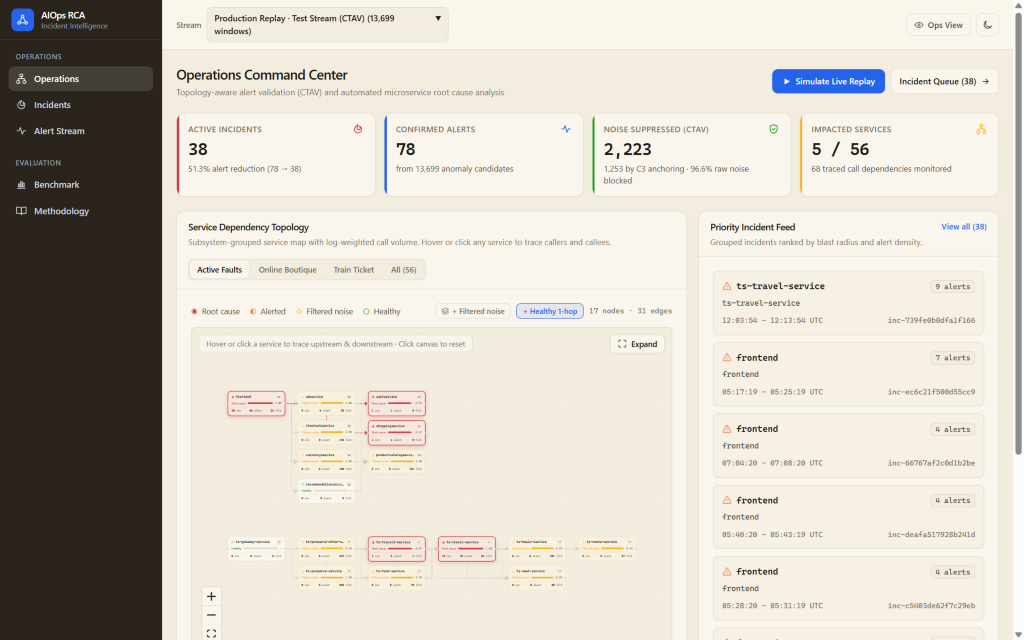
\includegraphics[width=\linewidth]{Images/C1/figures/m10-overview.png}
  \par\vspace{0.4cm}
  \caption[Màn hình Operations Command Center trên tập test]{Màn hình Operations Command Center giám sát đồ thị phụ thuộc 56 service và hàng đợi sự cố trên tập \splitname{test} (\code{pipeline\_test\_v2}).}
  \label{fig:ch6-overview}
\end{figure}

Màn hình trả lời câu hỏi định hướng đầu tiên của ca trực: \emph{trên toàn hệ thống microservice, những service nào đang phát sinh sự cố, bán kính ảnh hưởng trên đồ thị gọi rộng đến đâu và bộ thẩm định đã lọc bớt bao nhiêu nhiễu trước khi đẩy vào hàng đợi xử lý?} Trên lượt chạy \splitname{test}, bốn thẻ đầu trang cho thấy từ $13.699$ \code{candidate} bất thường, \CTAV{} chặn $2.223$ phán quyết dương tính thô ($96{,}6\%$, riêng \comp{C3} chặn $1.253$ ca), chỉ giữ lại $78$ cảnh báo xác nhận trên $5/56$ service và gom tiếp thành $38$ sự cố (mức giảm cảnh báo \term{ARR}{ARR} toàn cục đạt $51{,}3\%$). % src: pipeline_test_v2, rca_final_test_v1
Bản đồ đồ thị phân cụm tự động hai hệ OnlineBoutique và TrainTicket, quy đổi lưu lượng lời gọi theo thang logarit thành độ dày nét vẽ, đồng thời cung cấp bộ lọc nhanh theo vùng lỗi đang hoạt động (\emph{Active Faults}, rút gọn còn $17$ nút và $31$ cạnh lân cận 1-hop) cùng chế độ phóng toàn màn hình. Khi người vận hành nhấp chọn một nút bất kỳ trên đồ thị, ngăn tra cứu bên dưới lập tức liệt kê các service gọi đến (\emph{upstream callers}) và các service bị gọi (\emph{downstream callees}) để chuyển thẳng sang dòng cảnh báo đã lọc theo đúng service đó.

Về mặt phương pháp, màn hình này trực quan hóa trực tiếp đồ thị phụ thuộc \code{ServiceGraph} ($56$ nút, $68$ cạnh dựng từ trace) vốn đóng vai trò hạt nhân cho cả bước mở rộng vùng tìm 2-hop của \comp{C1} (Mục~\ref{sec:ch4-c1}) lẫn bước gom thành phần liên thông của tác tử \term{RCA}{RCA} (Mục~\ref{sec:ch4-grouping}).

\subsubsection{Alert Stream và Incidents: dòng cảnh báo phát lại và hàng đợi sự cố}
\label{sec:ch6-timeline}

Hình~\ref{fig:ch6-timeline} hiển thị màn hình \emph{Alert Stream \& Live Replay} (\code{/timeline}) của lượt chạy \code{pipeline\_test\_v2} khi bật lớp phủ đối chiếu nhãn chuẩn (\emph{Eval Overlay: ON}). Các cột xếp chồng gom $13.699$ \code{candidate} theo từng khung 10 phút và tô màu theo phán quyết cuối (xanh dương: \code{True Alert}, cam: \code{False Positive}, xanh ngọc: \code{Uncertain}); đường liền màu sẫm biểu diễn số cửa sổ lỗi thật theo nhãn Nezha. Người đọc nên đối chiếu vệt xanh dương rất mỏng ở đáy cột với các đỉnh của đường lỗi chuẩn, đồng thời chú ý thanh điều khiển phát lại (\emph{Simulate Live Replay}) ngay dưới tiêu đề trang.

\begin{figure}[htbp]
  \centering
  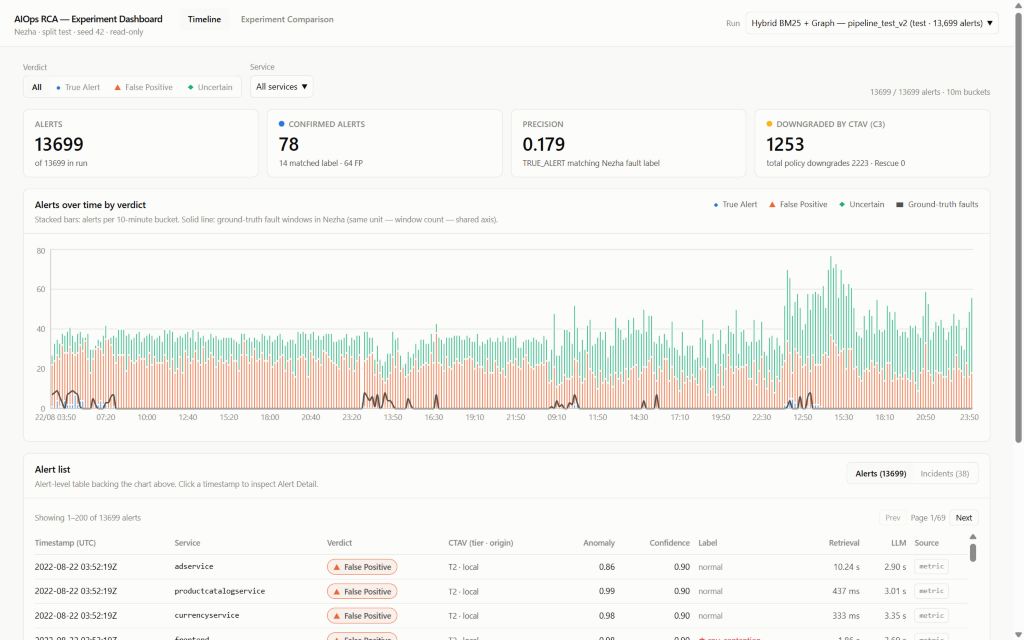
\includegraphics[width=\linewidth]{Images/C1/figures/m10-timeline.png}
  \par\vspace{0.4cm}
  \caption[Màn hình Alert Stream trên tập test]{Màn hình Alert Stream phát lại dòng phân loại $13.699$ cảnh báo đối chiếu nhãn chuẩn trên tập \splitname{test} (\code{pipeline\_test\_v2}).}
  \label{fig:ch6-timeline}
\end{figure}

Màn hình trả lời câu hỏi thứ hai của người vận hành: \emph{theo diễn tiến thời gian, lưu lượng cảnh báo ứng viên biến động ra sao và những cảnh báo xác nhận tập trung vào thời điểm nào?} Thanh điều khiển phát lại cho phép tua dòng cảnh báo từng bước ở tốc độ $1\times$, $3\times$, $10\times$ hoặc nhảy thẳng tới khung giờ có cảnh báo xác nhận kế tiếp (\emph{Next Confirmed Alert}), giúp tái hiện trực quan cách luồng cảnh báo đi qua bộ lọc \CTAV{} theo trật tự thời gian. Bên cạnh bảng cảnh báo phân trang 200 dòng, phân khu vận hành còn có màn hình hàng đợi sự cố chuyên biệt \emph{Incidents} (\code{/incidents}), nơi người trực ca lọc riêng các sự cố lan truyền đa service (\emph{Multi-service}) hoặc đơn service (\emph{Single-service}) và sắp xếp theo số lượng cảnh báo gom bên trong.

Nối với Chương~\ref{ch:de-xuat}, bốn thẻ chỉ số và biểu đồ cột phản ánh hiệu ứng kết hợp của ngưỡng \term{IF}{Isolation Forest}, bộ truy xuất \comp{C1} và cổng neo \comp{C3} (Mục~\ref{sec:ch4-policy}). Khi bật \emph{Eval Overlay}, màn hình cũng phơi bày trung thực giới hạn độ phủ mà Chương~\ref{ch:thuc-nghiem} đã chỉ ra: nhiều đỉnh của đường tiêm lỗi không có vạch xanh dương nào bên dưới. Đây chính là các đợt tiêm lỗi rơi vào nhóm $32/42$ service thiếu ngưỡng nền \splitname{dev}, nơi \comp{C3} hạ bậc toàn bộ cảnh báo do không có mốc tham chiếu cục bộ (Phát hiện 11, Mục~\ref{sec:ch5-finding11}).

\subsubsection{Alert Detail: vì sao giữ hay hạ một cảnh báo}
\label{sec:ch6-alert}

Hình~\ref{fig:ch6-alert} trình bày màn hình \emph{Alert Detail} của ứng viên \code{cand-ad327c0b162f6198} trên một cửa sổ bình thường của \code{productcatalogservice} (\code{pipeline\_test\_v2}). Người đọc nên đọc theo ba tầng từ trên xuống: hàng thẻ thông số và biểu đồ chuỗi điểm bất thường ở bên trái, lời giải thích của judge cùng bảng kiểm tra chính sách \CTAV{} ở cột phải, và thẻ giải thích ngữ cảnh \emph{How \comp{C1} built this context} trải rộng ở phần dưới.

\begin{figure}[htbp]
  \centering
  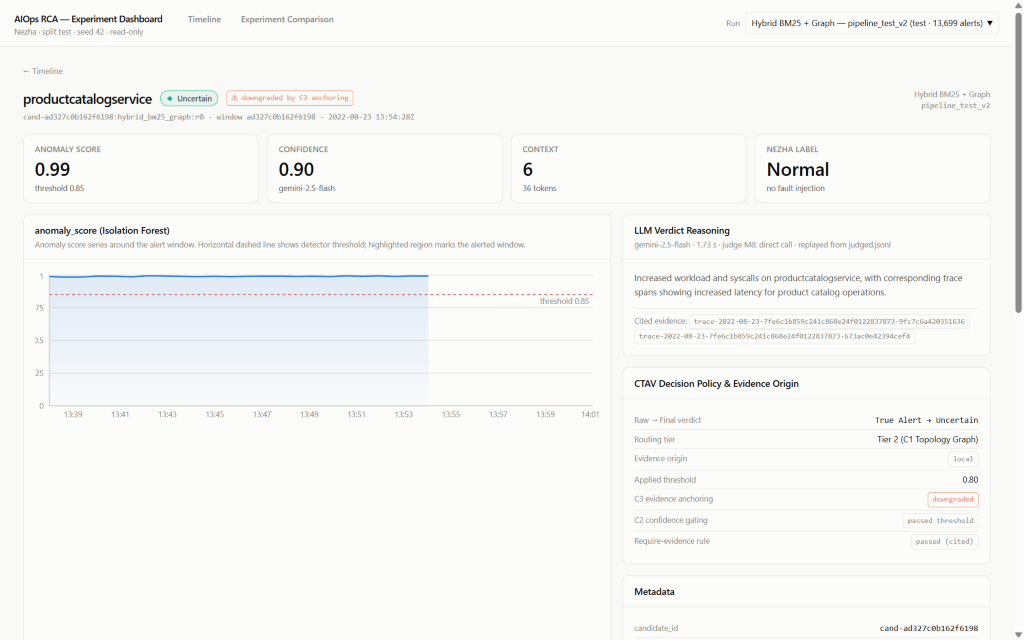
\includegraphics[width=\linewidth,height=0.72\textheight,keepaspectratio]{Images/C1/figures/m10-alert-c3-downgrade.png}
  \par\vspace{0.4cm}
  \caption[Màn hình Alert Detail giải thích ca bị C3 hạ bậc]{Màn hình Alert Detail giải thích ca báo động giả bị \comp{C3} hạ bậc và vùng ngữ cảnh \comp{C1} (\code{cand-ad327c0b162f6198}, \code{pipeline\_test\_v2}).}
  \label{fig:ch6-alert}
\end{figure}

Màn hình trả lời câu hỏi cốt lõi ở cấp độ từng cửa sổ: \emph{cùng mang điểm bất thường rất cao, vì sao hệ thống giữ lại cảnh báo này nhưng hạ bậc cảnh báo kia, và đồ thị phụ thuộc đã đóng góp gì vào bộ bằng chứng mà judge đọc?} Ở cột phải của Hình~\ref{fig:ch6-alert}, người vận hành thấy nguyên văn lập luận của \code{gemini-2.5-flash} viện dẫn hai span trace cục bộ để kết luận độ trễ tăng, tiếp theo là bảng thực thi tuần tự ba quy tắc chính sách: luật bắt buộc trích dẫn bằng chứng (\code{passed}), ngưỡng tin cậy $\theta = 0{,}80$ (\code{passed threshold}) và bước neo \comp{C3} (\code{downgraded}). Vì cả hai span được trích dẫn đều có thời gian thực thi nằm dưới phân vị $p_{90}$ của \splitname{dev}, \comp{C3} bác bỏ kết luận cảm tính của judge và hạ phán quyết xuống \code{Uncertain}. % src: m10_demo_cases_v1 step2

Đây là nơi cơ chế hiệu chỉnh của Mục~\ref{sec:ch4-policy} và \term{ConfirmationBias}{thiên lệch xác nhận} ở Phát hiện 7 (Bảng~\ref{tab:ch5-findings}) hiện ra trực tiếp trên dữ liệu thật. Thẻ \emph{How \comp{C1} built this context} ở nửa dưới Hình~\ref{fig:ch6-alert} giải thích minh bạch vai trò của đồ thị ở tầng truy xuất: nửa trái chia vùng tìm thành ba dải khoảng cách $d = 0, 1, 2$ trên đồ thị gọi vô hướng (tương ứng $1$, $3$ và $6$ service quanh \code{productcatalogservice}); nửa phải vẽ thanh thành phần \term{FusionScore}{Fusion Score} gồm $0{,}35 \times \mathrm{BM25}$, $0{,}25 \times$ độ gần thời gian và $0{,}40 \times 1/(1+d)$ đúng theo Công thức~\eqref{eq:ch4-fusion}, kèm viền cam quanh bằng chứng được judge trích dẫn. Cả sáu sự kiện lọt vào top-6 đều thuộc chính \code{productcatalogservice} ($d = 0$), vì một sự kiện cách 1 hop đã chịu mức phạt $0{,}20$ điểm ở thành phần đồ thị. Thẻ không tô vẽ kịch bản ``service lân cận cứu cảnh báo'', nhất quán với thực tế trên \code{pipeline\_test\_v2} chỉ có $75/19.794$ bằng chứng ($0{,}38\%$, thuộc $15/3.299$ cảnh báo có ngữ cảnh) đến từ service lân cận. % src: scripts/m11_graph_evidence_share.py --run-id pipeline_test_v2

\subsubsection{Incident Detail: định vị service gốc và đồ thị lân cận}
\label{sec:ch6-incident}

Hình~\ref{fig:ch6-incident} trình bày màn hình \emph{Incident Detail} của sự cố đa service \code{inc-46289ea526eaa3f3}, lấy từ luồng độ nhạy ngoài đăng ký \code{pipeline\_sens\_test\_v1} (biến thể \comp{C3} dùng ngưỡng nền trượt 60 phút) do lượt chạy đăng ký trên \splitname{test} không sinh ra cụm sự cố đa service nào. Người đọc nên chú ý hai dải băng vàng cảnh báo chế độ độ nhạy ở đầu trang, thẻ kể chuyện ba bước \emph{How the \term{RCA}{RCA} agent localized the root cause} ở giữa, cùng đồ thị lân cận ngang (\emph{Service Neighborhood Graph}) đặt cạnh báo cáo chẩn đoán JSON ở nửa dưới.

\begin{figure}[htbp]
  \centering
  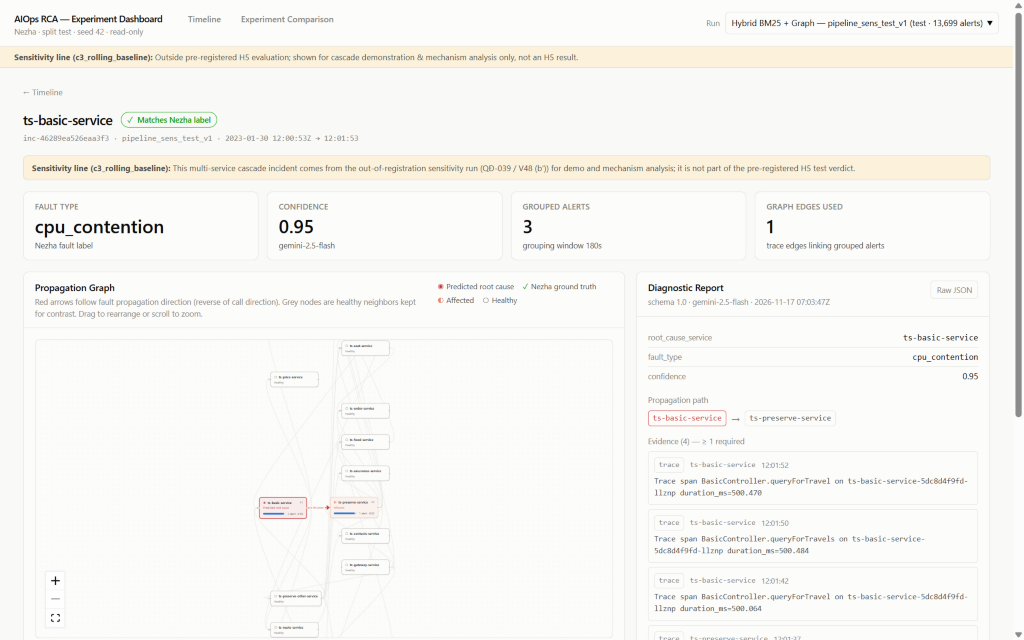
\includegraphics[width=\linewidth,height=0.72\textheight,keepaspectratio]{Images/C1/figures/m10-incident-cascade.png}
  \par\vspace{0.4cm}
  \caption[Màn hình Incident Detail định vị sự cố đa service]{Màn hình Incident Detail định vị service gốc ba bước và hiển thị đồ thị lan truyền của sự cố \code{inc-46289ea526eaa3f3} (\code{pipeline\_sens\_test\_v1}).}
  \label{fig:ch6-incident}
\end{figure}

Màn hình trả lời câu hỏi của khâu điều tra sự cố: \emph{khi nhiều cảnh báo nổ đồng thời trên các service liên kết nhau, lỗi phát sinh từ đâu, thuật toán suy diễn thứ hạng thế nào và gợi ý xử lý dựa trên bằng chứng nào?} Thẻ ba bước ở giữa tách bạch phần định vị hoàn toàn tất định (không dùng \term{LLM}{LLM}) thành ba khung có thể bấm chọn từng bước: (1)~trục thời gian gom ba cảnh báo trong khoảng cách $\le 180\,\text{s}$; (2)~sơ đồ các service có cảnh báo nối bởi mũi tên xám chỉ chiều gọi trong trace (\code{ts-preserve-service} gọi \code{ts-basic-service} $465$ lần) và mũi tên đỏ nét đứt chỉ chiều lỗi lan ngược, kèm các service hạ nguồn khỏe mạnh để thấy lý do dừng lan truyền; (3)~bảng chia phiếu bầu lùi một bước kết luận \code{ts-basic-service} đạt điểm tuyệt đối $1{,}00$, khớp nhãn gốc \code{cpu\_contention} của Nezha. % src: m10_demo_cases_v1 step4

Ở nửa dưới bên trái, đồ thị \emph{Service Neighborhood Graph} bố trí chuỗi lan truyền chính nằm ngang trên trục trung tâm (mũi tên đỏ liền nét từ \code{\#1 ts-basic-service} sang \code{\#2 ts-preserve-service}), tách các service gọi đến lên hàng trên và các service bị gọi xuống hàng dưới; chế độ mặc định \emph{Propagation Focus} giữ tối đa ba lân cận khỏe mạnh mỗi phía để sơ đồ thoáng rõ, có thể mở rộng toàn bộ qua nút \emph{Full 1-Hop (+9)} hoặc phóng toàn màn hình. Khung bên phải hiển thị báo cáo JSON đã vượt qua năm quy tắc kiểm duyệt ở Mục~\ref{sec:ch4-report}, gồm bốn trích đoạn trace kèm thời gian thực thi và ba khuyến nghị khắc phục phân mức ưu tiên. Như đã nhấn mạnh ở Mục~\ref{sec:ch5-rca-results}, ca này minh họa cơ chế gom và định vị của nhánh B vận hành đúng khi có đủ cảnh báo đầu vào, hoàn toàn không thay đổi kết luận \hyp{H5} không được chấp nhận trên luồng đăng ký chính thức ($38$ sự cố đơn service). % src: rca_final_test_v1

\subsubsection{Benchmark và Methodology: đối chiếu kiểm định và sổ tay phương pháp}
\label{sec:ch6-compare}

Hình~\ref{fig:ch6-compare} là màn hình \emph{Benchmark} (\code{/compare}), mặc định mở kết quả chính thức trên tập \splitname{test} và cho phép chuyển nhanh sang tập \splitname{val} để tham chiếu chéo. Dải cảnh báo vàng của luồng độ nhạy được tự động ẩn trên phân khu đánh giá để tránh gây nhầm lẫn với số liệu đăng ký. Người đọc nên nhìn bốn ô tóm tắt chỉ số đầu trang cùng cột trạng thái ba màu của bảng kiểm định \hyp{H0}--\hyp{H5}.

\begin{figure}[htbp]
  \centering
  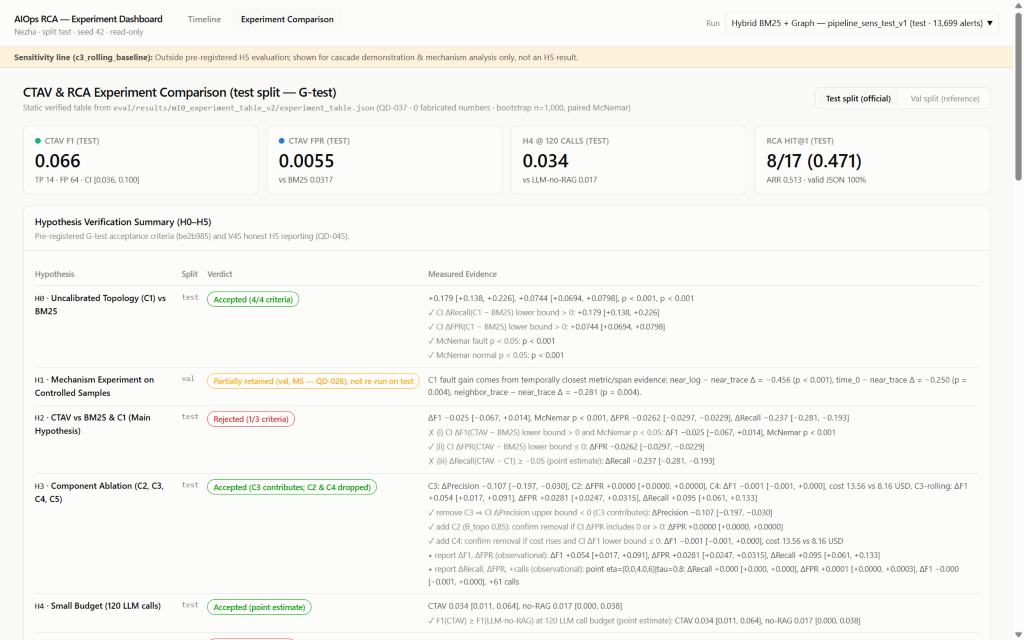
\includegraphics[width=\linewidth]{Images/C1/figures/m10-experiment-comparison.png}
  \par\vspace{0.4cm}
  \caption[Màn hình Benchmark tổng hợp kiểm định H0--H5]{Màn hình Benchmark (\code{/compare}) đối chiếu kết quả kiểm định \hyp{H0}--\hyp{H5} trên tập \splitname{test}.}
  \label{fig:ch6-compare}
\end{figure}

Màn hình trả lời câu hỏi của hội đồng thẩm định khoa học: \emph{khi đặt \CTAV{} cạnh các đường cơ sở theo đúng bản đăng ký giả thuyết trên \splitname{test}, giả thuyết nào được chấp nhận và giả thuyết nào bị bác bỏ?} Bên dưới bảng tổng hợp sáu giả thuyết là biểu đồ cột năm phương pháp kèm râu CI95 bootstrap, bảng hiệu ghép cặp kèm trị số $p$ của kiểm định McNemar, bảng ablation \hyp{H3} tích hợp điểm thử \comp{C5}, đường cong ngân sách \hyp{H4} và bảng kết quả \term{RCA}{RCA} của \hyp{H5} đặt cạnh dòng độ nhạy \code{C3-rolling}. Đi kèm màn hình này trong phân khu đánh giá là trang \emph{Methodology} (\code{/guide}), đóng vai trò sổ tay tra cứu tại chỗ trình bày trọn vẹn bốn công thức toán học của từng tầng xử lý, lý do loại bỏ các mô-đun âm (\comp{C2}, \comp{C4}, \comp{C5}) và bảng giải nghĩa thuật ngữ thống kê để phục vụ trực tiếp phiên hỏi đáp với hội đồng. Hai màn hình này nối thẳng với toàn bộ Chương~\ref{ch:thuc-nghiem} và là phiên bản tương tác của Bảng~\ref{tab:ch5-verdict-summary}.

% -----------------------------------------------------------------------------
\subsection{Kịch bản demo năm phút}
\label{sec:ch6-kich-ban}

Mục này chuẩn hóa kịch bản trình diễn năm bước trong thời lượng năm phút trước hội đồng. Toàn bộ mã ứng viên và mã sự cố trong kịch bản đều được rút tự động bằng quy tắc xác định (\code{seed = 42}) từ kho kết quả đã khóa của \splitname{test} và \splitname{val}, thay vì chọn thủ công; chẳng hạn ca ở bước 2 được lấy ngẫu nhiên có hạt giống từ tập $1.171$ cửa sổ bình thường trên \splitname{test} mà judge thô đánh nhãn \code{TRUE\_ALERT} nhưng bị \comp{C3} chặn lại. % src: m10_demo_cases_v1
Người trình bày có thể đi qua năm bước bằng cách bấm trực tiếp menu \emph{Guided Scenarios} ở chân thanh bên trái, giúp tự động đồng bộ đúng tham số \code{run\_id} và tự bật lớp phủ \emph{Eval Overlay} ở các bước đối chiếu nhãn.

Hai điểm điều chỉnh thực tế khi ánh xạ từ thiết kế sang dữ liệu thật được thuyết minh thẳng thắn ngay trong buổi demo. Thứ nhất, ở bước 3 về lỗi \code{network\_delay} mà \CTAV{} giữ được còn \term{BM25}{BM25} bỏ sót: trên \splitname{val}, \CTAV{} đánh rơi cả $10$ ca \code{network\_delay} của \comp{C1}, nhưng trên \splitname{test} có đúng $2$ ca thỏa mãn tiêu chí (\code{cartservice} và \code{ts-travel-service}). % src: ctav_final_val_v1, ctav_final_test_v1
Ở cả hai ca này, toàn bộ bằng chứng được chọn đều nằm ngay tại service phát cảnh báo ($d_G = 0$), nên thông điệp chính xác của bước 3 là \comp{C1} xếp hạng đúng span trễ cục bộ và \comp{C3} neo giữ thành công, chứ không phải ``nhờ log từ service lân cận''. Thứ hai, ở bước 4 về sự cố lan truyền nhiều service: luồng đăng ký \code{pipeline\_test\_v2} không có sự cố đa service nào, còn đợt tiêm lỗi \code{2023-01-30\#009} trên \code{pipeline\_val\_v2} lại bị tách thành hai sự cố đơn lẻ do service trung gian không phát cảnh báo để nối cạnh đồ thị. Kịch bản vì vậy chuyển sang luồng độ nhạy \code{pipeline\_sens\_test\_v1} (có dải băng vàng cảnh báo ngoài đăng ký) để trình diễn thuật toán định vị 3 bước, rồi đối chiếu ngay với ca bị tách đôi trên \splitname{val} để giải thích trực quan vì sao \hyp{H5} không đạt. Bảng~\ref{tab:ch6-kich-ban} tóm tắt năm bước thao tác.

\begin{table}[H]
  \centering
  \caption[Kịch bản demo năm phút trên giao diện điều hành]{Kịch bản demo năm phút trên bộ ca chọn tự động (\code{seed = 42}), chạy hoàn toàn ngoại tuyến với \code{DEMO\_OFFLINE=1}.}
  \label{tab:ch6-kich-ban}
  \tblfont
  \tblsetup
  \setlength{\tabcolsep}{3.5pt}
  \begin{tabularx}{\linewidth}{|>{\raggedright\arraybackslash}p{2.4cm}|>{\raggedright\arraybackslash}p{3.8cm}|Y|>{\raggedright\arraybackslash}p{3.3cm}|}
    \hline
    \rowcolor{gray!15}
    \textbf{Bước (thời lượng)} & \textbf{Thao tác} & \textbf{Người xem thấy} & \textbf{Thông điệp} \\
    \hline
    1. Toàn cảnh \& Dòng cảnh báo ($\approx 60$~s) & Mở \code{/overview} rồi sang \code{/timeline} của \code{pipeline\_test\_v2} (bật \emph{Eval Overlay}) & Bản đồ $56$ service ($5$ service có sự cố), chặn $96{,}6\%$ nhiễu thô ($2.223$ ca, riêng \comp{C3} hạ $1.253$ ca); còn $78$ \code{TRUE\_ALERT} $\to 38$ sự cố; tua nhanh thanh \emph{Live Replay} & Platform chạy khép kín ngoại tuyến ($4{,}24$~s từ cache); \CTAV{} nén mạnh báo động giả nhưng hụt đỉnh ở service thiếu ngưỡng \splitname{dev} \\
    \hline
    2. Chặn báo động giả nhờ \comp{C3} ($\approx 60$~s) & Chọn Kịch bản~2 (\code{cand-ad327c0b\allowbreak 162f6198}) mở Alert Detail & \code{productcatalogservice}, nhãn chuẩn \code{Normal}, điểm bất thường $0{,}99$; judge thô trả \code{True Alert} ($0{,}90$), thẻ chính sách ghi \comp{C3} hạ xuống \code{Uncertain}; thẻ \comp{C1} hiện đủ $6$ bằng chứng ở $d = 0$ & Neo định lượng $p_{90}$ chặn hiệu quả \term{ConfirmationBias}{thiên lệch xác nhận} trên trace cục bộ \\
    \hline
    3. Ca \code{network\_\allowbreak delay} \term{BM25}{BM25} bỏ sót ($\approx 60$~s) & Chọn Kịch bản~3 (\code{cand-fa85e82f\allowbreak 02f08574}) mở Alert Detail & \code{cartservice}: \term{BM25}{BM25} phán nhầm \code{False Positive} ($0{,}90$); \CTAV{} giữ \code{True Alert} nhờ span \code{CartService/GetCart} vượt ngưỡng \splitname{dev} (\code{anchored}); cả $6$ sự kiện ở $d = 0$ & \comp{C1} đưa đúng span trễ vào ngữ cảnh và \comp{C3} bảo toàn tín hiệu thật ($1$ trong $2$ ca trên \splitname{test}) \\
    \hline
    4. Sự cố cascade \& giới hạn \hyp{H5} ($\approx 75$~s) & Chọn Kịch bản~4 (\code{inc-46289ea5\allowbreak 26eaa3f3}, \code{pipeline\_sens\_\allowbreak test\_v1}); đối chiếu ca tách \code{2023-01-30\#009} trên \code{pipeline\_val\_v2} & Hai dải vàng ngoài đăng ký; thẻ 3 bước bỏ phiếu chấm \code{ts-basic-service} đạt $1{,}00$ khớp nhãn gốc; đồ thị trục ngang và JSON hợp lệ; trên \splitname{val} cùng đợt lỗi bị tách làm hai & Tác tử \term{RCA}{RCA} gom cụm và định vị đúng khi đủ cảnh báo; \hyp{H5} không đạt do độ phủ cảnh báo đầu vào thưa \\
    \hline
    5. Bảng kiểm định \& Sổ tay ($\approx 45$~s) & Mở \code{/compare} (chuyển thử \splitname{test}/\splitname{val}) và lướt \code{/guide} & Bảng \hyp{H0}--\hyp{H5} kèm CI95, đường cong ngân sách \hyp{H4}, bảng ablation \hyp{H3} + \comp{C5} và công thức bốn tầng ở \code{/guide} & \comp{C3} là đóng góp cốt lõi; \comp{C2}, \comp{C4} bị loại, \comp{C5} không mang lại lợi ích ròng; báo cáo trung thực cả \hyp{H2} và \hyp{H5} không đạt \\
    \hline
  \end{tabularx}
\end{table}

% -----------------------------------------------------------------------------
\subsection{Kiểm thử demo và dự phòng}
\label{sec:ch6-kiem-thu}

Mục này xác minh ba yêu cầu kỹ thuật của nền tảng trình diễn: vận hành hoàn toàn không cần Internet, bảo toàn tính nhất quán tuyệt đối với số liệu kiểm định, và có độ trễ khởi tạo đủ ngắn cho phiên bảo vệ. Bảng~\ref{tab:ch6-kiem-thu-dulieu} đối chiếu quy mô bản ghi, mức khớp kiểm chứng (\emph{parity}) và tỷ lệ trúng cache của ba lượt chạy được nạp vào cơ sở dữ liệu, còn Bảng~\ref{tab:ch6-kiem-thu-thoigian} phân rã thời gian thực thi đầu--cuối theo từng khâu. Cần lưu ý rằng thời gian trong Bảng~\ref{tab:ch6-kiem-thu-thoigian} là thời gian đọc lại từ cache trên đĩa và ghi vào hai kho lưu trữ, không phải độ trễ suy luận trực tuyến qua mạng; độ trễ gốc của từng lời gọi \term{LLM}{LLM} vẫn được bảo toàn nguyên vẹn trong ClickHouse để tra cứu ở màn hình Alert Detail.

\begin{table}[H]
  \centering
  \caption[Kiểm thử chạy ngoại tuyến: quy mô bản ghi, đối chiếu và cache]{Kiểm thử chạy ngoại tuyến của ba lượt chạy pipeline (phần 1): số bản ghi nạp, đối chiếu với kết quả kiểm định và tỷ lệ trúng cache.}
  \label{tab:ch6-kiem-thu-dulieu}
  \tblfont
  \tblsetup
  \setlength{\tabcolsep}{3.5pt}
  \begin{tabularx}{\linewidth}{|Y|>{\raggedright\arraybackslash}p{3.0cm}|>{\raggedright\arraybackslash}p{3.1cm}|>{\raggedright\arraybackslash}p{3.4cm}|}
    \hline
    \rowcolor{gray!15}
    \textbf{Chỉ số dữ liệu \& đối chiếu} & \textbf{\code{pipeline\_val\_v2} (\splitname{val})} & \textbf{\code{pipeline\_test\_v2} (\splitname{test})} & \textbf{\code{pipeline\_sens\_\allowbreak test\_v1} (\splitname{test}, độ nhạy ngoài ĐK)} \\
    \hline
    \code{candidate} nạp / \code{TRUE\_ALERT} & $5.677$ / $80$ & $13.699$ / $78$ & $13.699$ / $438$ \\
    \hline
    Dòng bằng chứng trong ClickHouse & $7.716$ & $19.794$ & $19.794$ \\
    \hline
    Sự cố / báo cáo hợp lệ (bị từ chối) & $26$ / $26$ ($0$) & $38$ / $38$ ($0$) & $114$ / $114$ ($0$) \\
    \hline
    Đối chiếu sự cố, thứ hạng, báo cáo với lượt kiểm định & $26/26$ & $38/38$ & $114/114$ \\
    \hline
    Lần gọi API mới / tỷ lệ trúng cache & $0$ / $100\%$ & $0$ / $100\%$ & $0$ / $100\%$ \\
    \hline
    Token judge trong cache (prompt / completion) & $5.173.670$ / $691.941$ & $12.736.820$ / $1.734.808$ & $12.736.820$ / $1.734.808$ \\
    \hline
  \end{tabularx}
\end{table}

\begin{table}[H]
  \centering
  \caption[Kiểm thử chạy ngoại tuyến: phân rã thời gian thực thi đầu--cuối]{Kiểm thử chạy ngoại tuyến của ba lượt chạy pipeline (phần 2): phân rã thời gian thực thi từng khâu khi nạp lại từ cache.}
  \label{tab:ch6-kiem-thu-thoigian}
  \tblfont
  \tblsetup
  \setlength{\tabcolsep}{3.5pt}
  \begin{tabularx}{\linewidth}{|Y|>{\raggedright\arraybackslash}p{3.0cm}|>{\raggedright\arraybackslash}p{3.1cm}|>{\raggedright\arraybackslash}p{3.4cm}|}
    \hline
    \rowcolor{gray!15}
    \textbf{Khâu thực thi} & \textbf{\code{pipeline\_val\_v2} (\splitname{val})} & \textbf{\code{pipeline\_test\_v2} (\splitname{test})} & \textbf{\code{pipeline\_sens\_\allowbreak test\_v1} (\splitname{test}, độ nhạy ngoài ĐK)} \\
    \hline
    Nạp cảnh báo và chính sách & $0{,}62$~s & $1{,}25$~s & $5{,}28$~s \\
    \hline
    Ghi ClickHouse & $2{,}90$~s & $1{,}27$~s & $2{,}79$~s \\
    \hline
    Gom sự cố và lan truyền & $4$~ms & $6$~ms & $19$~ms \\
    \hline
    Tóm tắt báo cáo (đọc cache) & $0{,}42$~s & $0{,}44$~s & $0{,}71$~s \\
    \hline
    Ghi PostgreSQL & $0{,}33$~s & $0{,}19$~s & $0{,}35$~s \\
    \hline
    \textbf{Tổng thời gian đầu--cuối} & $\mathbf{5{,}76}$~\textbf{s} & $\mathbf{4{,}24}$~\textbf{s} & $\mathbf{10{,}65}$~\textbf{s} \\
    \hline
  \end{tabularx}
\end{table}
% src: eval/results/{pipeline_val_v2,pipeline_test_v2,pipeline_sens_test_v1}/runtime.json
% Doi chieu: rca_final_val_v1, rca_final_test_v1, rca_sens_test_c3rolling_v1

Cả ba lượt chạy đều khớp $100\%$ với kết quả kiểm định gốc ở Chương~\ref{ch:thuc-nghiem} trên cả danh sách cảnh báo thành viên, thứ hạng service gốc lẫn mã băm nội dung báo cáo JSON, với $0$ lần gọi API mới. Luồng kiểm thử chính thức \code{pipeline\_test\_v2} hoàn tất nạp dữ liệu sau $4{,}24$~s, trong đó riêng thuật toán gom cụm và bỏ phiếu lan truyền của tác tử \term{RCA}{RCA} chỉ mất $6$~ms (và không quá $19$~ms ở luồng độ nhạy $438$ cảnh báo).

Kiểm thử vận hành thực tế được thực hiện ở hai lớp độc lập. Ở lớp kiểm thử tự động, bộ kiểm thử hợp đồng xác nhận toàn bộ tám endpoint (bao gồm \code{GET /topology}) trả đúng lược đồ dữ liệu trên cả ClickHouse lẫn PostgreSQL thật, kiểm chứng cơ chế xóa khóa API khi bật \code{DEMO\_OFFLINE=1}, đồng thời chạy bộ kiểm thử khói kết xuất phía máy chủ trên cả năm màn hình, các hàm suy diễn chính sách \comp{C3} và bộ xếp bố cục đồ thị. Ở lớp kiểm duyệt trình duyệt thật (tổng duyệt lần hai ngày 25/11/2026 sau khi nâng cấp giao diện điều hành), trình duyệt Chromium mở trực tiếp \code{http://localhost:5173} đi trọn năm màn hình của Bảng~\ref{tab:ch6-kich-ban}: toàn bộ trang tải hoàn tất với $0$ lỗi console, $0$ kết nối ra ngoài \code{localhost} và mọi truy vấn nội bộ đều trả mã HTTP 200. Các tồn đọng giao diện ghi nhận ở đợt tổng duyệt đầu tiên cũng đã được xử lý trọn vẹn: (i)~bộ hình Hình~\ref{fig:ch6-overview}--\ref{fig:ch6-compare} đã cập nhật đầy đủ thẻ giải thích \comp{C1}, thẻ ba bước \term{RCA}{RCA} và đồ thị phụ thuộc; (ii)~trục thời gian của Alert Stream tự động lặp lại tiền tố ngày \code{dd/MM} mỗi khi qua mốc nửa đêm; (iii)~dải băng vàng của luồng độ nhạy được cô lập khỏi phân khu đánh giá; và (iv)~mã nguồn giao diện được tách mảnh theo từng tuyến màn hình (\emph{code splitting}), giảm gói khởi tạo chính xuống còn khoảng $46$~kB ($\approx 16$~kB sau nén gzip) và triệt tiêu cảnh báo kích thước gói khi đóng gói. Trên thẻ phiếu bầu \term{RCA}{RCA}, $177/178$ sự cố của cả ba lượt chạy khớp trực tiếp điểm bầu từ cạnh gọi; duy nhất một sự cố hòa điểm $0{,}50$ được hệ thống phá hòa bằng điểm bất thường cực đại và gắn chú thích minh bạch ngay trên thẻ.

Phương án dự phòng cho buổi bảo vệ được thiết kế hai mức. Ở mức một, nếu một container gặp sự cố tức thời, lệnh \code{docker compose --profile dev up -d} khởi tạo lại dịch vụ mà không ảnh hưởng dữ liệu lưu bền vững trong volume. Ở mức hai, phòng trường hợp máy trình chiếu gặp trục trặc môi trường Docker, toàn bộ ba lượt chạy (\code{pipeline\_test\_v2}, \code{pipeline\_val\_v2}, \code{pipeline\_sens\_test\_v1}) đã được kết xuất sẵn sang ảnh chụp API tĩnh (\code{VITE\_DATA\_SOURCE=static}, đóng gói bảng \code{alerts} dạng cột nén giảm khoảng $65\%$ dung lượng cùng trọn bộ chi tiết sự cố, cảnh báo mẫu và đồ thị \code{topology}). Nhờ cơ chế này, toàn bộ năm màn hình của giao diện vẫn mở và tương tác trực tiếp được từ tệp tĩnh trên trình duyệt (hoặc bản triển khai tĩnh trên GitHub Pages) mà không cần Docker hay cơ sở dữ liệu chạy nền, bên cạnh bộ năm ảnh chụp độ phân giải 300~dpi lưu sẵn.

% -----------------------------------------------------------------------------
\subsection{Kết chương}
\label{sec:ch6-ket-chuong}

Chương này đã trình bày nền tảng trình diễn hiện thực hóa trọn vẹn chuỗi xử lý của đề tài, từ \code{candidate} của bộ phát hiện qua \CTAV{} và tác tử \term{RCA}{RCA} tới tám endpoint chỉ đọc và giao diện năm màn hình tách bạch giữa điều hành trực ca với đối chiếu kiểm định. Vì dùng chung đường ống thực thi với harness nghiên cứu, mọi con số và ca bệnh trên màn hình đều khớp $100\%$ với kết quả đã kiểm định ở Chương~\ref{ch:thuc-nghiem}, nạp lại hoàn toàn từ cache sau $4{,}24$--$10{,}65$~s mà không phát sinh bất kỳ lời gọi API hay kết nối mạng bên ngoài nào. Mỗi màn hình giải quyết một câu hỏi cụ thể và gắn trực tiếp với thiết kế ở Chương~\ref{ch:de-xuat}: Operations với bức tranh đồ thị phụ thuộc toàn hệ, Alert Stream với diễn tiến nén nhiễu theo thời gian, Alert Detail với cơ chế neo định lượng \comp{C3} và vùng tìm \comp{C1}, Incident Detail với ba bước định vị của tác tử \term{RCA}{RCA}, cùng Benchmark và Methodology với bảng kiểm định \hyp{H0}--\hyp{H5}. Kịch bản demo năm phút sử dụng bộ ca chọn tự động theo hạt giống cố định, đồng thời kết hợp chế độ snapshot tĩnh không phụ thuộc Docker để bảo đảm an toàn trình diễn ở mọi điều kiện phòng họp. Chương~\ref{ch:thao-luan} tiếp theo đi sâu phân tích cơ chế và phân loại toàn bộ các ca sai đứng sau những giới hạn đã quan sát trên nền tảng này.

 \newpage
 % =============================================================================
% Chuong 7: Thao luan (chuan lop article cho Internship2_HK262)
% Nguon noi dung: docs/drafts/ch7-phan-tich-ca-sai.md (7.3-7.5),
%   docs/drafts/suon-bao-cao-gd2.md (7.1-7.2), Ch5_ThucNghiemVaDanhGia.tex,
%   eval/results/m11_error_analysis_test_v1/{error_analysis.json,tables.md},
%   eval/results/m8_detector_shift_test_v1/shift.json, eval/results/m8_finding11_test_v1/finding11.json
% Cho M11: muc 7.4.4 (cham mu diagnostic_quality.csv) va mot cau o 7.5.
% =============================================================================

\section{Thảo luận}
\label{ch:thao-luan}

Chương~\ref{ch:thuc-nghiem} đã trả lời giả thuyết nào đạt và giả thuyết nào không. Chương này trả lời ba câu hỏi tiếp theo: các kết quả đó có nghĩa gì, đáng tin tới đâu, và hệ thống sai ở những ca nào. Chương không lặp lại bảng số của Chương~\ref{ch:thuc-nghiem}; mỗi luận điểm chỉ trích một hai con số rồi giải thích nguyên nhân. Mục~\ref{sec:ch7-tong-hop} tổng hợp các kết quả chính cùng mức độ tin cậy của từng kết quả. Mục~\ref{sec:ch7-thao-luan} giải thích vì sao \comp{C3} (neo bằng chứng) có tác dụng còn \comp{C2} (ngưỡng bất đối xứng), \comp{C4} (định tuyến hai tầng) và \comp{C5} (\term{RescueScore}{Rescue Score}) thì không. Mục~\ref{sec:ch7-hop-le} rà soát các mối đe doạ tính hợp lệ, và Mục~\ref{sec:ch7-ca-sai} phân tích toàn bộ ca sai trên \splitname{test} của \CTAV{} và tác tử \term{RCA}{RCA}. Hạn chế của hệ thống và hướng phát triển được để lại cho Chương~\ref{ch:tong-ket}.

% -----------------------------------------------------------------------------
\subsection{Tổng hợp kết quả chính}
\label{sec:ch7-tong-hop}

Mục này gom kết quả của Chương~\ref{ch:thuc-nghiem} thành năm khẳng định và đánh giá mức tin cậy của từng khẳng định. Tiêu chí tin cậy ở đây gồm hai phần: kết quả có lặp lại cùng chiều giữa \splitname{val} và \splitname{test} hay không, và khoảng tin cậy có đủ hẹp để loại trừ giá trị $0$ hay không. Bảng~\ref{tab:ch7-tong-hop} trình bày năm khẳng định; người đọc nên nhìn cột cuối để biết khẳng định nào có thể dùng như kết luận và khẳng định nào chỉ nên đọc như giải thích cơ chế.

\begin{table}[H]
  \centering
  \caption[Năm khẳng định chính và mức độ tin cậy]{Năm khẳng định chính rút ra từ Chương~\ref{ch:thuc-nghiem}, bằng chứng trên \splitname{test} (\term{TelemetryWindow}{cửa sổ có telemetry}: $11.985$ cửa sổ, $346$ lỗi), đối chiếu \splitname{val} ($7.636$ cửa sổ, $209$ lỗi) và mức độ tin cậy.}
  \label{tab:ch7-tong-hop}
  \tblfont
  \tblsetup
  \setlength{\tabcolsep}{3.5pt}
  \begin{tabularx}{\linewidth}{|>{\raggedright\arraybackslash}p{3.4cm}|Y|>{\raggedright\arraybackslash}p{2.7cm}|>{\raggedright\arraybackslash}p{2.6cm}|}
    \hline
    \rowcolor{gray!15}
    \textbf{Khẳng định} & \textbf{Bằng chứng chính trên \splitname{test}} & \textbf{Trên \splitname{val}} & \textbf{Mức tin cậy} \\
    \hline
    (1) Thêm ngữ cảnh topology chưa hiệu chỉnh (\comp{C1}) tăng cả recall lẫn báo động giả & $96$ so với $34$ TP; $1.235$ so với $369$ FP; McNemar $p < 0{,}001$ ở cả hai nhãn & Cùng chiều, biên độ nhỏ hơn & Cao: lặp lại, CI loại trừ $0$ \\
    \hline
    (2) Báo động giả của judge đến từ trace cục bộ sát thời điểm cảnh báo, không từ service lân cận & Chỉ $0{,}38\%$ bằng chứng của \comp{C1} đến từ service lân cận; $63/64$ FP còn lại của \CTAV{} dùng bằng chứng cục bộ & Thí nghiệm can thiệp \hyp{H1} (chỉ chạy trên \splitname{val}) & Trung bình: cơ chế đo trên \splitname{val}, \splitname{test} chỉ có bằng chứng quan sát \\
    \hline
    (3) Neo bằng chứng (\comp{C3}) giảm mạnh báo động giả & \comp{C3} cắt $1.171/1.235$ FP của \comp{C1} ($94{,}8\%$); \term{FPR}{FPR} của \CTAV{} $0{,}0055$ so với $0{,}0317$ của \term{BM25}{BM25} & Cùng chiều (giảm \term{FPR}{FPR} $8$ lần so với \term{BM25}{BM25}) & Cao: lặp lại, CI loại trừ $0$ \\
    \hline
    (4) \CTAV{} với ngưỡng nền \splitname{dev} cố định không giữ được recall & Recall $0{,}040$; \comp{C3} hạ $82/96$ TP của \comp{C1}, trong đó $67$ TP ở service thiếu ngưỡng \splitname{dev} & Recall thấp hơn \comp{C1}, F1 vẫn cao nhất & Cao: nguyên nhân định lượng được (Phát hiện 11) \\
    \hline
    (5) Tác tử \term{RCA}{RCA} chỉ định vị tốt bằng chất lượng cảnh báo đầu vào & $\text{Hit@1} = 0{,}471$, bằng baseline; $29/50$ lần tiêm không có cảnh báo & $\text{Hit@1} = 0{,}636$, bằng baseline & Thấp: chỉ $17$ sự cố có nhãn, CI rộng \\
    \hline
  \end{tabularx}
\end{table}
% src: ctav_final_test_v1, h0_test_*, m8_finding11_test_v1, rca_final_test_v1, pipeline_test_v2 (graph evidence share)

Khẳng định (1) và (3) là hai kết quả vững nhất của luận văn. Cả hai lặp lại cùng chiều trên hai split độc lập, và khoảng tin cậy không chứa $0$. Chúng cho thấy một đánh đổi rõ ràng: ngữ cảnh rộng hơn giúp judge thấy nhiều sự cố hơn, nhưng cũng khiến judge xác nhận nhiều cửa sổ bình thường hơn; và một chính sách quyết định có kiểm chứng bằng chứng gỡ được phần lớn báo động giả này. Khẳng định (4) là kết quả âm nhưng cũng là kết quả có giá trị. Nó đảo chiều kết luận \hyp{H2} từ ``đạt một phần'' trên \splitname{val} thành ``không được chấp nhận'' trên \splitname{test}, và Chương~\ref{ch:thuc-nghiem} đã định lượng được nguyên nhân: $32/42$ service của \splitname{test} không có ngưỡng nền \splitname{dev}. % src: m8_finding11_test_v1
Khẳng định (5) có độ tin cậy thấp nhất vì cỡ mẫu nhỏ, nên chỉ nên đọc như một quan sát về giới hạn của kiến trúc, không như một ước lượng chính xác về khả năng định vị.

% -----------------------------------------------------------------------------
\subsection{Thảo luận: vì sao \comp{C3} có tác dụng, vì sao \comp{C2}, \comp{C4}, \comp{C5} thì không}
\label{sec:ch7-thao-luan}

Mục này giải thích cơ chế đứng sau kết quả ablation \hyp{H3}, thay vì chỉ ghi nhận thành phần nào được giữ. Năm thành phần được nhắc theo đúng chức năng đã định nghĩa ở Chương~\ref{ch:de-xuat}: \comp{C1} (truy xuất lai \term{BM25}{BM25}--topology, đang dùng), \comp{C2} (gating theo nguồn bằng chứng, đã loại), \comp{C3} (neo bằng chứng, đang dùng), \comp{C4} (định tuyến hai tầng, đã loại) và \comp{C5} (\term{RescueScore}{Rescue Score}, chỉ là ablation).

\subsubsection{Vì sao \comp{C3} có tác dụng}
\label{sec:ch7-c3}

\comp{C3} có tác dụng vì nó kiểm đúng chỗ mà judge yếu. Thí nghiệm \hyp{H1} trên \splitname{val} cho thấy judge rất nhạy với trace của chính service đang xét khi trace nằm sát thời điểm cảnh báo: chỉ đưa loại bằng chứng này vào ngữ cảnh làm tỷ lệ \code{TRUE\_ALERT} trên cửa sổ bình thường lên $60{,}8\%$, so với $18{,}1\%$ khi chỉ đưa log cục bộ. % src: h1_val (Mục ch5-h1)
Judge không phân biệt ``có một span chậm'' với ``span đó chậm bất thường''. \comp{C3} bổ sung đúng phép so sánh còn thiếu: mỗi span được judge trích dẫn phải vượt ngưỡng $p_{90}$ của cùng thao tác trên \splitname{dev}, nếu không thì phán quyết bị hạ xuống \code{UNCERTAIN}. Nói cách khác, \comp{C3} không thay judge ra quyết định; nó buộc lý do của judge phải có cơ sở định lượng.

Hai quan sát khác giải thích vì sao không thể thay \comp{C3} bằng một ngưỡng tin cậy chặt hơn. Thứ nhất, khi thiếu ngữ cảnh, độ tin cậy mà judge tự báo gần như chép lại \code{anomaly\_score} của detector (Phát hiện 2), và trên \splitname{val} nó chỉ nhận vài giá trị rời rạc như $0{,}80$, $0{,}85$, $0{,}90$. Trên \splitname{test}, cả $64/64$ báo động giả còn lại đều có độ tin cậy $0{,}9$, nên không ngưỡng $\theta$ nào tách được chúng khỏi cảnh báo thật. % src: m11_error_analysis_test_v1
Thứ hai, trên Nezha, việc \emph{có} bằng chứng đã gần như trùng với việc ở gần sự cố: mọi cửa sổ lỗi đều có telemetry, trong khi chỉ khoảng $25\%$ cửa sổ bình thường có (Phát hiện 1). Một chính sách chỉ đòi ``có bằng chứng'' vì thế sẽ học nhầm quy luật thu thập dữ liệu thay vì học dấu hiệu lỗi; \comp{C3} đòi bằng chứng \emph{bất thường}, một điều kiện không phụ thuộc quy luật đó.

Điểm yếu của \comp{C3} nằm ở nguồn ngưỡng, không nằm ở nguyên lý. Khi chỉ thay ngưỡng \splitname{dev} cố định bằng ngưỡng trượt 60 phút không cần nhãn (\code{C3-trượt}), F1 trên \splitname{test} tăng từ $0{,}066$ lên $0{,}120$, $\Delta\text{F1} = +0{,}054$ $[+0{,}017;\, +0{,}091]$. % src: h3_test c3_rolling_baseline
Kết quả này là bằng chứng mạnh nhất cho thấy ý tưởng neo bằng chứng đúng, còn cách hiện thực ngưỡng nền thì quá mong manh trước độ lệch thành phần service giữa các split. Cần lưu ý \code{C3-trượt} là biến thể đối chứng trong \hyp{H3}, không phải cấu hình đã đăng ký cho \hyp{H2}, nên nó không thay đổi kết luận \hyp{H2}.

\subsubsection{Vì sao \comp{C2} và \comp{C4} bị loại}
\label{sec:ch7-c2-c4}

\comp{C2} được thiết kế dựa trên giả thuyết ban đầu: báo động giả của \comp{C1} đến từ bằng chứng của service lân cận, nên cần ngưỡng tin cậy chặt hơn cho bằng chứng loại này. Thí nghiệm \hyp{H1} bác bỏ giả thuyết đó (Phát hiện 7): báo động giả đến từ trace cục bộ, và trace lân cận còn ít gây xác nhận hơn ($27{,}7\%$ so với $60{,}8\%$ trên cửa sổ bình thường của \splitname{val}). Vì \comp{C2} nhắm vào một nguyên nhân không tồn tại, tác động của nó gần như bằng $0$. Trên \splitname{val}, \comp{C2} chỉ bớt $2$ FP với CI của $\Delta\text{FPR}$ chạm $0$; trên \splitname{test}, cả $54$ cảnh báo mà \comp{C2} hạ đều đã bị \comp{C3} chặn từ trước, nên không phán quyết cuối nào thay đổi. % src: h3_val, h3_test
Đây là một ví dụ của nguyên tắc ``đổi hướng có ghi lại'': thành phần bị loại vì giả thuyết thiết kế của nó sai, và luận văn giữ lại bằng chứng của việc loại đó.

\comp{C4} bị loại vì một lý do khác: chi phí. Thiết kế định tuyến hai tầng dựa trên giả định rằng tầng \term{BM25}{BM25} rẻ sẽ xử lý xong phần lớn \code{candidate} và chỉ chuyển lên \comp{C1} các ca khó. Giả định này không đúng trên Nezha, vì chính tầng \term{BM25}{BM25} sinh nhiều báo động giả và tỷ lệ leo thang lên tầng 2 cao (Phát hiện 9). Trên \splitname{test}, thêm \comp{C4} làm tăng $3.286$ lượt gọi LLM ($13{,}56$ so với $8{,}16$ USD quy đổi) và thêm $4$ FP mà không thêm TP nào. % src: h3_test add_c4
Kết quả này nhất quán giữa \splitname{val} và \splitname{test}, nên quyết định loại \comp{C4} có độ tin cậy cao.

\subsubsection{Vì sao \comp{C5} không thêm recall}
\label{sec:ch7-c5}

\comp{C5} nhắm vào một nguồn bỏ sót có thật: trên \splitname{test}, detector để lọt $122$ cửa sổ lỗi có telemetry dưới ngưỡng $0{,}85$. Tuy nhiên, cứu thêm \code{candidate} chỉ có ích khi các tầng phía sau xác nhận được chúng. Ở điểm tham số đã chốt, \comp{C5} vớt lên $61$ cửa sổ trên \splitname{test}, trong đó $3$ cửa sổ lỗi, và cả $3$ đều bị judge trả \code{FALSE\_POSITIVE} trước khi tới \comp{C3}; kết quả cuối là $+0$ TP và $+1$ FP. % src: c5_test (Mục ch5-test-c5)
Nút thắt của recall vì vậy không nằm ở cổng \code{candidate} mà nằm ở khả năng phân biệt của judge, như phân tích ca bỏ sót ở Mục~\ref{sec:ch7-fn} cho thấy: $128$ cửa sổ lỗi đã vào được tới judge với đủ sáu sự kiện ngữ cảnh nhưng vẫn bị bác. Phát hiện này đúng trên cả hai split (Phát hiện 12), nên \comp{C5} được giữ như một kết quả ablation âm, không bật trong cấu hình chính.

% -----------------------------------------------------------------------------
\subsection{Mối đe doạ tính hợp lệ}
\label{sec:ch7-hop-le}

Mục này rà soát các yếu tố có thể làm kết luận của Chương~\ref{ch:thuc-nghiem} sai lệch, theo bốn nhóm: tính hợp lệ nội tại, bên ngoài, cấu trúc phép đo và kết luận thống kê. Bảng~\ref{tab:ch7-hop-le-noitai} trình bày nhóm mối đe doạ tính hợp lệ nội tại, còn Bảng~\ref{tab:ch7-hop-le-khac} tổng hợp ba nhóm còn lại kèm biện pháp kiểm soát và rủi ro còn lại. Hai yếu tố ảnh hưởng mạnh nhất tới việc đọc số giữa \splitname{val} và \splitname{test} là độ lệch tỷ lệ \code{candidate} của detector và việc ngưỡng nền của \comp{C3} được cố định trên \splitname{dev}; người đọc nên đọc hàng thứ ba của Bảng~\ref{tab:ch7-hop-le-noitai} trước.

\begin{table}[H]
  \centering
  \caption[Mối đe doạ tính hợp lệ nội tại, biện pháp và rủi ro còn lại]{Mối đe doạ tính hợp lệ nội tại (phần 1), biện pháp kiểm soát đã áp dụng và rủi ro còn lại đối với kết luận.}
  \label{tab:ch7-hop-le-noitai}
  \tblfont
  \tblsetup
  \setlength{\tabcolsep}{4pt}
  \begin{tabularx}{\linewidth}{|>{\raggedright\arraybackslash}p{4.1cm}|Y|>{\raggedright\arraybackslash}p{4.2cm}|}
    \hline
    \rowcolor{gray!15}
    \textbf{Mối đe doạ nội tại} & \textbf{Biện pháp đã áp dụng} & \textbf{Rủi ro còn lại} \\
    \hline
    Rò nhãn: truy vấn \term{BM25}{BM25} ban đầu chứa từ khoá loại lỗi; telemetry chỉ có ở khoảng $25\%$ cửa sổ bình thường so với $100\%$ cửa sổ lỗi & Xoá thẻ loại lỗi khỏi truy vấn \term{BM25}{BM25} và \comp{C1}, có kiểm thử tự động chặn; chấm chỉ số chính trên \term{TelemetryWindow}{cửa sổ có telemetry} & Cửa sổ bình thường có telemetry vẫn tập trung quanh các phút tiêm lỗi, khác lưu lượng sản xuất liên tục \\
    \hline
    Dữ liệu và mô hình: cột \code{PodSuccessRate(\%)} luôn bằng $0$ khiến judge hiểu nhầm; nhà cung cấp có thể đổi ngầm phiên bản mô hình & Loại cột lỗi khỏi bản tóm tắt metric; cố định \code{gemini-2.5-flash}, nhiệt độ $0$, kiểm \code{modelVersion} trong từng bản ghi cache & Quy tắc làm sạch đặc thù cho Nezha; kết quả gắn với một phiên bản mô hình thương mại \\
    \hline
    Chọn cấu hình sau hai lần nhìn \splitname{val}; detector lệch khi sang \splitname{test}: tỷ lệ \code{candidate} từ $19{,}6\%$ lên $29{,}2\%$ & Đăng ký \hyp{H0}--\hyp{H5} và khoá cấu hình (\code{be2b985}) trước khi chạy \splitname{test} đúng một lần; tách số \splitname{val} (chọn cấu hình) khỏi \splitname{test} (kiểm định) & $32/42$ service của \splitname{test} ($61{,}0\%$ cửa sổ lỗi) không có ngưỡng \splitname{dev}; đây là nguyên nhân trực tiếp làm \hyp{H2} không đạt \\
    \hline
  \end{tabularx}
\end{table}

\begin{table}[H]
  \centering
  \caption[Mối đe doạ tính hợp lệ bên ngoài, phép đo và thống kê]{Mối đe doạ tính hợp lệ bên ngoài, cấu trúc phép đo và kết luận thống kê (phần 2), biện pháp kiểm soát và rủi ro còn lại.}
  \label{tab:ch7-hop-le-khac}
  \tblfont
  \tblsetup
  \setlength{\tabcolsep}{3.5pt}
  \begin{tabularx}{\linewidth}{|>{\raggedright\arraybackslash}p{1.8cm}|>{\raggedright\arraybackslash}p{3.6cm}|Y|>{\raggedright\arraybackslash}p{3.8cm}|}
    \hline
    \rowcolor{gray!15}
    \textbf{Nhóm} & \textbf{Mối đe doạ} & \textbf{Biện pháp đã áp dụng} & \textbf{Rủi ro còn lại} \\
    \hline
    Bên ngoài & Một bộ dữ liệu (Nezha, hai hệ), một judge, chạy phát lại từ cache & Ghi rõ phạm vi ở mọi kết luận; báo kết quả tách theo hệ và theo năm loại lỗi & Chưa kiểm chứng ngưỡng $\theta = 0{,}80$, ngưỡng $p_{90}$ hay hành vi của judge trên dữ liệu, lưu lượng hoặc họ LLM khác \\
    \hline
    Cấu trúc phép đo & Nhãn cửa sổ theo khoảng quanh thời điểm tiêm; Hit@$k$ chấm mức service trên nhãn gốc mức pod; ngưỡng $\delta = 0{,}05$ của \hyp{H2} chọn sau khi xem \splitname{val}; nhãn chất lượng ngữ cảnh do quy tắc ngưỡng gán, nhãn chất lượng báo cáo do LLM chấm nháp & Chia split theo lần tiêm lỗi với vùng đệm $600$~s; công bố rõ việc chấm mức service dễ hơn mức pod; bảng chấm mù, tách khoá nhãn; báo kết quả nhạy theo ngưỡng; tác giả rà soát trước khi mở khoá & Cửa sổ bình thường sát sự cố có thể chịu lan truyền thật trên trace ($31/64$ FP còn lại của \CTAV{}); quy tắc ngưỡng thiên về \comp{C1}; không có người chấm độc lập thứ hai, mẫu $30$ báo cáo cho CI rộng \\
    \hline
    Kết luận thống kê & Không hiệu chỉnh đa so sánh cho \hyp{H0}, \hyp{H1}, \hyp{H3}, \hyp{H4}; phương sai judge chỉ đo trên $200$ cửa sổ; \hyp{H5} chỉ có $17$ sự cố có nhãn & Bootstrap ghép cặp $1.000$ mẫu (\code{seed = 42}), McNemar chính xác trên cùng tập cửa sổ; không kết luận khác biệt khi CI chứa $0$ & Suy diễn cho các giả thuyết phụ và \hyp{H5} có độ bất định lớn ($\text{Hit@1}$ CI95 $[0{,}235;\, 0{,}706]$) \\
    \hline
  \end{tabularx}
\end{table}
% src: experiment-log (dang ky be2b985), m8_detector_shift_test_v1/shift.json, m8_finding11_test_v1/finding11.json, rca_final_test_v1

Biện pháp quan trọng nhất trong bảng là việc đăng ký trước và chạy \splitname{test} đúng một lần. Nhờ đó, sự sụt giảm của \CTAV{} trên \splitname{test} được báo cáo như nó xảy ra, thay vì bị che đi bằng một lần chỉnh tham số nữa. Độ ổn định của judge cũng không phải mối lo chính: qua ba lần gọi độc lập trên $200$ \code{candidate} của \splitname{test}, tỷ lệ lật nhãn chỉ $0{,}005$--$0{,}010$ và không cửa sổ lỗi nào bị lật (Mục~\ref{sec:ch5-repeat}). % src: repeat_test_v1
Hai phép đánh giá chất lượng ngoài kiểm định \hyp{H0}--\hyp{H5} có giới hạn riêng về cách gán nhãn, và cần được đọc cùng giới hạn đó. Chỉ số chất lượng ngữ cảnh (Mục~\ref{sec:ch5-context-precision}) dùng nhãn do quy tắc ngưỡng gán, không do người chấm. Quy tắc thưởng cho span chậm gần cửa sổ, đúng thứ thành phần độ gần thời gian của \comp{C1} tối ưu ($76\%$ sự kiện của \comp{C1} nằm trong $\pm 180$~s so với $58\%$ của \term{BM25}{BM25}), nên hiệu $+0{,}073$ giữa \comp{C1} và \term{BM25}{BM25} thiên về phía \comp{C1} và không được dùng làm bằng chứng so sánh. % src: m8_context_precision_v2
Chất lượng báo cáo chẩn đoán (Mục~\ref{sec:ch7-human}) do một LLM khác họ với judge chấm nháp trên bảng mù rồi tác giả rà soát, nên không phải đánh giá độc lập của con người và không có hệ số đồng thuận giữa hai người chấm.

% -----------------------------------------------------------------------------
\subsection{Phân tích ca sai}
\label{sec:ch7-ca-sai}

Mục này phân loại toàn bộ ca sai còn lại trên \splitname{test} của \CTAV{} (cấu hình đóng băng: \comp{C1}, $\theta = 0{,}80$ và \comp{C3} với ngưỡng $p_{90}$ của \splitname{dev}) và của tác tử \term{RCA}{RCA}, không chỉnh tham số nào sau khi xem kết quả. Bảng~\ref{tab:ch7-ca-sai-ctav} tổng hợp $64$ báo động giả và $332$ sự cố bị bỏ sót của \CTAV{} trên $11.985$ \term{TelemetryWindow}{cửa sổ có telemetry}, còn Bảng~\ref{tab:ch7-ca-sai-rca} phân loại các ca định vị sai của tác tử \term{RCA}{RCA} ở cả lượt chạy đăng ký lẫn dòng độ nhạy. Người đọc nên chú ý cột cuối: mỗi nhóm ca sai gắn với một đặc điểm định lượng, và các đặc điểm này là cơ sở cho hạn chế cùng hướng phát triển ở Chương~\ref{ch:tong-ket}.

\begin{table}[H]
  \centering
  \caption[Phân loại ca sai của CTAV trên tập test]{Phân loại $64$ báo động giả và $332$ sự cố bị bỏ sót của \CTAV{} trên \splitname{test} (\term{TelemetryWindow}{cửa sổ có telemetry}: $11.985$ cửa sổ, $346$ lỗi).}
  \label{tab:ch7-ca-sai-ctav}
  \tblfont
  \tblsetup
  \setlength{\tabcolsep}{3.5pt}
  \begin{tabularx}{\linewidth}{|>{\raggedright\arraybackslash}p{1.2cm}|>{\raggedright\arraybackslash}p{4.3cm}|r|r|Y|}
    \hline
    \rowcolor{gray!15}
    \textbf{Mã} & \textbf{Nhóm ca sai} & \textbf{Số ca} & \textbf{Tỷ lệ} & \textbf{Đặc điểm định lượng chính} \\
    \hline
    \multicolumn{5}{|l|}{\textbf{\CTAV{} --- $64$ báo động giả} (chỉ ở \code{frontend}: $39$, \code{ts-travel-service}: $25$)} \\
    \hline
    FP-1 & Trùng thời gian với lỗi tiêm ở service phía sau & 31 & 48,4\% & Trung vị độ trễ span neo $= 3{,}02 \times p_{90}$ của \splitname{dev} (tối đa $68{,}78\times$) \\
    \hline
    FP-2 & Ngoài mọi lần tiêm lỗi & 33 & 51,6\% & Trung vị $1{,}95 \times p_{90}$ (tối đa $7{,}60\times$) \\
    \hline
    \multicolumn{5}{|l|}{\textbf{\CTAV{} --- $332$ sự cố bị bỏ sót} ($346 - 14$ TP; recall $0{,}040$)} \\
    \hline
    FN-1 & Detector không đưa lên \code{candidate} (điểm $< 0{,}85$) & 122 & 36,7\% & \code{network\_delay} $62$, \code{return} $27$, \code{exception} $23$, \code{cpu\_contention} $10$ \\
    \hline
    FN-2 & Judge trên ngữ cảnh \comp{C1} trả \code{FALSE\_POSITIVE} & 128 & 38,6\% & Cả $128$ ca đủ $6$ sự kiện ngữ cảnh; $64$ có / $64$ không có ngưỡng \splitname{dev} \\
    \hline
    FN-3a & \comp{C3} hạ: service không có ngưỡng \splitname{dev} & 67 & 20,2\% & Rơi vào $8$ service, nhiều nhất \code{checkoutservice} ($17$) \\
    \hline
    FN-3b & \comp{C3} hạ: thao tác không có ngưỡng \splitname{dev} & 3 & 0,9\% & Đều ở \code{ts-travel-service}; có $2$ span mức \code{WARN} trên $1.000$~ms \\
    \hline
    FN-3c & \comp{C3} hạ: span được trích nằm dưới $p_{90}$ & 12 & 3,6\% & Không có log \code{ERROR}/\code{WARN} cục bộ \\
    \hline
  \end{tabularx}
\end{table}

\begin{table}[H]
  \centering
  \caption[Phân loại ca sai định vị của tác tử RCA trên tập test]{Phân loại ca định vị sai của tác tử \term{RCA}{RCA} trên \splitname{test} ở lượt chạy đăng ký và dòng độ nhạy ngoài đăng ký.}
  \label{tab:ch7-ca-sai-rca}
  \tblfont
  \tblsetup
  \setlength{\tabcolsep}{3.5pt}
  \begin{tabularx}{\linewidth}{|>{\raggedright\arraybackslash}p{1.2cm}|>{\raggedright\arraybackslash}p{4.3cm}|r|r|Y|}
    \hline
    \rowcolor{gray!15}
    \textbf{Mã} & \textbf{Nhóm ca sai} & \textbf{Số ca} & \textbf{Tỷ lệ} & \textbf{Đặc điểm định lượng chính} \\
    \hline
    \multicolumn{5}{|l|}{\textbf{Tác tử \term{RCA}{RCA}, lượt chạy đăng ký} ($38$ sự cố, $17$ có nhãn; $9$ ca trượt \term{HitK}{Hit@1})} \\
    \hline
    R1 & Lỗi ở service bị gọi trực tiếp, chỉ service gọi có cảnh báo & 7 & 7/9 & \code{frontend} thay cho \code{checkoutservice}, \code{currencyservice}; \code{ts-travel-service} thay cho \code{ts-basic-service}, \code{ts-route-service} \\
    \hline
    R2 & Lỗi cách từ hai bước trở lên hoặc không có cạnh gọi & 2 & 2/9 & \code{frontend} so với \code{paymentservice}; \code{ts-travel-service} so với \code{ts-security-service} \\
    \hline
    \multicolumn{5}{|l|}{\textbf{Tác tử \term{RCA}{RCA}, dòng độ nhạy ngoài đăng ký} ($114$ sự cố, $48$ có nhãn; $38$ ca trượt \term{HitK}{Hit@1})} \\
    \hline
    S1 & Service gốc không có cảnh báo trong sự cố & 33 & 33/38 & $21$ ở xa hoặc không có cạnh; $6$ là service bị gọi; $6$ là service gọi \\
    \hline
    S2 & Service gốc có cảnh báo nhưng bị xếp sau & 5 & 5/38 & Cả $5$ đều trúng \term{HitK}{Hit@3}; $3$ do phiếu dồn về service bị gọi, $2$ do hoà phiếu \\
    \hline
  \end{tabularx}
\end{table}
% src: eval/results/m11_error_analysis_test_v1/error_analysis.json

\subsubsection{Báo động giả còn lại của \CTAV{}}
\label{sec:ch7-fp}

Trên \splitname{test}, \comp{C1} sinh $1.235$ báo động giả và \comp{C3} loại được $1.171$, để lọt $64$. Cả $64$ ca có chung một kiểu kích hoạt: judge trả \code{TRUE\_ALERT} với độ tin cậy $0{,}9$, và ít nhất một span cục bộ được trích vượt $p_{90}$ của \splitname{dev}, nên \comp{C3} không có lý do để hạ. Không ca nào được neo bằng log \code{ERROR} hay \code{WARN}, và $63/64$ ca chỉ dùng bằng chứng của chính service. % src: m11_error_analysis_test_v1
Các báo động giả cũng chỉ rơi vào hai service cửa ngõ có ngưỡng \splitname{dev}: \code{frontend} và \code{ts-travel-service}. Điều này gắn trực tiếp với độ lệch của detector: trên \splitname{test}, detector đánh dấu \code{candidate} cho $100\%$ cửa sổ của \code{frontend} ($1.221/1.221$), một service không xuất hiện trong \splitname{val}. % src: m8_detector_shift_test_v1
Khi hàng trăm cửa sổ bình thường của service cửa ngõ liên tục đi qua \comp{C1}, chỉ cần một span gọi ra ngoài có đuôi dài là đủ để cả judge lẫn \comp{C3} coi đó là dấu hiệu sự cố.

Đối chiếu thời điểm với $50$ lần tiêm lỗi chia $64$ ca thành hai nhóm gần bằng nhau nhưng khác nguyên nhân. Nhóm FP-1 ($31$ ca) xảy ra trong lúc lỗi đang được tiêm ở một service phía sau, chủ yếu \code{network\_delay} ($20/31$). Ở đây span của service cửa ngõ thật sự chậm vì phải chờ phản hồi. Ví dụ, cửa sổ \code{f07889584e1176e6} của \code{frontend} có span \code{CartService/GetCart} $23{,}932$~ms so với $p_{90} = 7{,}689$~ms, trong lúc \code{checkoutservice} đang bị tiêm \code{network\_delay}. Theo quy ước nhãn chỉ gắn cho pod bị tiêm, các ca này là báo động giả; về nghiệp vụ, chúng là ảnh hưởng thật của sự cố và một người vận hành vẫn muốn biết. Nhóm FP-2 ($33$ ca) nằm ngoài mọi lần tiêm và có độ vượt ngưỡng thấp hơn hẳn (trung vị $1{,}95\times$). Đây là nhược điểm cấu trúc của ngưỡng phân vị đơn lẻ: theo định nghĩa, khoảng $10\%$ span bình thường đã vượt $p_{90}$, nên một luật chỉ đòi một span vượt ngưỡng sẽ luôn để lọt một phần dao động thường ngày.

\subsubsection{Sự cố bị bỏ sót của \CTAV{}}
\label{sec:ch7-fn}

$332$ cửa sổ lỗi bị bỏ sót phân bố khá đều qua ba tầng nối tiếp: detector ($122$), judge ($128$) và \comp{C3} ($82$). Không ca nào bị loại bởi luật bắt buộc có bằng chứng hay ngưỡng tin cậy $\theta$. Phân bố này cho thấy không có một sửa đổi đơn lẻ nào nâng được recall đáng kể; mỗi tầng chặn khoảng một phần ba.

Ở tầng detector (FN-1), một nửa số ca bỏ sót là \code{network\_delay} ($62/122$). Lỗi độ trễ mạng và lỗi tầng ứng dụng (\code{return}, \code{exception}) ít để lại dấu vết trên các chỉ số tài nguyên mà Isolation Forest dùng; một số service như \code{ts-verification-code-service} bị bỏ sót toàn bộ $21/21$ cửa sổ lỗi. Ở tầng judge (FN-2), cả $128$ cửa sổ đều có đủ sáu sự kiện ngữ cảnh, nhưng judge vẫn kết luận metric bị nhiễu, thường vì các span \code{INFO} trong top-6 có độ dài bình thường. Ví dụ, cửa sổ \code{0731855dab245bad} của \code{frontend} có \code{anomaly\_score} $0{,}984$ khi đang bị tiêm \code{cpu\_contention}, nhưng judge trả \code{FALSE\_POSITIVE} với độ tin cậy $0{,}9$. Nguyên nhân có khả năng là \term{FusionScore}{Fusion Score} xếp các span nhẹ của request khác lên đầu, và lỗi \code{return}, \code{exception} không phải lúc nào cũng ghi log \code{ERROR} trong sáu sự kiện đó.

Ở tầng \comp{C3}, ba nguyên nhân con có quy mô rất khác nhau. Lớn nhất là FN-3a ($67$ ca): service không có ngưỡng \splitname{dev}, nên mọi phán quyết đúng của judge trên $8$ service này đều bị hạ; đây chính là Phát hiện 11. FN-3b chỉ có $3$ ca nhưng lộ ra một lỗ hổng của luật neo: hai span \code{WARN} của \code{ts-travel-service} dài $1.469{,}73$~ms và $2.037{,}95$~ms vẫn bị hạ, vì luật \comp{C3} chỉ xét cờ \code{WARN} trên log, còn với trace thì đòi cặp (service, thao tác) phải có mặt trong \splitname{dev}. FN-3c ($12$ ca) cho thấy một giới hạn khác: \comp{C3} chỉ kiểm span mà judge chọn trích, nên khi judge đúng hướng nhưng chọn span đại diện nằm dưới $p_{90}$, cảnh báo vẫn bị hạ dù cửa sổ có span khác bất thường hơn.

\subsubsection{Ca sai của tác tử \term{RCA}{RCA}}
\label{sec:ch7-rca-sai}

Trên lượt chạy đăng ký, $78$ cảnh báo của \CTAV{} chỉ nằm trên $5$ service và tạo $38$ sự cố, tất cả đều chỉ có một service. Khi sự cố chỉ có một service, bước lan truyền ngược một bước không có cạnh nào để đi, nên luôn trả về chính service phát cảnh báo; vì vậy $\text{Hit@1} = \text{Hit@3}$ và bằng đúng baseline. Cả $9/17$ sự cố định vị sai đều cùng một dạng: service gốc không có cảnh báo. Trong $7$ ca (R1), lỗi nằm ở service bị gọi trực tiếp, còn cảnh báo chỉ bật ở service gọi phía trước do phải chờ phản hồi; đây chính là mặt bên kia của nhóm FP-1 ở Mục~\ref{sec:ch7-fp}. Hai ca còn lại (R2) có service gốc cách xa từ hai bước hoặc không có cạnh gọi trong đồ thị. Ngoài ra, $29/50$ lần tiêm lỗi hoàn toàn không có cảnh báo nào để định vị. % src: rca_final_test_v1, m11_error_analysis_test_v1

Dòng độ nhạy ngoài đăng ký giúp tách ảnh hưởng của đầu vào khỏi thuật toán. Với $438$ cảnh báo trên $22$ service, số lần tiêm không có cảnh báo giảm từ $29$ xuống $1$, nhưng $38/48$ sự cố có nhãn vẫn trượt \term{HitK}{Hit@1}. Trong đó $33$ ca (S1) vẫn do service gốc không nằm trong tập service có cảnh báo của sự cố; điều này đặt trần $15/48 = 0{,}313$ cho bất kỳ thuật toán nào chỉ xếp hạng trên tập đó. Chỉ $5$ ca (S2) là lỗi thật của thuật toán bỏ phiếu, và cả $5$ đều trúng \term{HitK}{Hit@3}. Ba trong số đó lộ ra giả định một chiều của lan truyền ngược: khi lỗi ở service gọi làm cả service bị gọi cũng bật cảnh báo, phiếu dồn về service bị gọi. Ví dụ, trong sự cố \code{inc-bd062ac615eaf3d7}, \code{frontend} bị tiêm \code{cpu\_contention} nhưng nhận $0$ phiếu vì không service nào gọi tới nó. % src: rca_sens_test_c3rolling_v1

Về tầng sinh báo cáo, mọi báo cáo đều hợp lệ về lược đồ JSON, nhưng nội dung có ba khiếm khuyết. Thứ nhất, mọi sự cố không ứng với lỗi nào ($18$ trên lượt đăng ký) vẫn được gán một loại lỗi cụ thể, vì bộ tóm tắt không có bước kiểm lại sự cố có thật hay không. Thứ hai, loại lỗi lệch nặng về \code{cpu\_contention} ($35/38$ báo cáo), nên chỉ đúng loại lỗi ở $5/17 = 29{,}4\%$ sự cố có nhãn; prompt tóm tắt có xu hướng diễn giải các đặc trưng CPU và syscall trong danh sách metric bất thường. Thứ ba, $1/38$ báo cáo đăng ký và $4/114$ báo cáo độ nhạy có chèn mã bằng chứng tự bịa, và bộ kiểm duyệt đã lọc bỏ toàn bộ. % src: m11_error_analysis_test_v1

\subsubsection{Đánh giá chất lượng nội dung báo cáo chẩn đoán}
\label{sec:ch7-human}

Tỷ lệ JSON hợp lệ $1{,}000$ chỉ đo cấu trúc, không đo nội dung chẩn đoán có đúng và dùng được hay không. Để đo phần này, $30$ trong $38$ sự cố của lượt chạy đăng ký được lấy mẫu ngẫu nhiên (\code{seed = 42}). Bảng chấm chỉ giữ tóm tắt cảnh báo, lập luận của judge, service và loại lỗi dự đoán, bằng chứng trích dẫn và gợi ý xử lý; mọi nhãn gốc được tách sang một tệp khoá riêng. Mỗi báo cáo được chấm theo ba tiêu chí, thang $0$--$2$: đúng nguyên nhân gốc, bằng chứng hợp lệ và gợi ý xử lý dùng được. Mức $1$ của tiêu chí nguyên nhân gốc chỉ dành cho trường hợp bất thường nằm ở service gọi hoặc bị gọi trực tiếp; bằng chứng cách cửa sổ quá $180$~s không được tính là chứng minh cho cửa sổ.

Quy trình chấm cần được nói rõ vì nó không phải đánh giá độc lập của con người. Một LLM khác họ với judge (\code{deepseek-flash}) chấm nháp cả $30$ dòng trên bảng mù. Tác giả rà soát toàn bộ bảng nháp, xem lại $10$ dòng có cách hiểu thang chấm chưa nhất quán và sửa điểm ở $9$ dòng, rồi mới mở tệp khoá để đối chiếu. Vì chỉ có một chuỗi chấm, luận văn không báo hệ số đồng thuận Cohen's $\kappa$. Bảng~\ref{tab:ch7-human} trình bày kết quả; người đọc nên so cột phân bố của tiêu chí gợi ý xử lý với hai tiêu chí còn lại.

\begin{table}[H]
  \centering
  \caption[Chất lượng nội dung báo cáo chẩn đoán trên mẫu 30 sự cố]{Chất lượng nội dung báo cáo chẩn đoán trên mẫu $30$ sự cố của \code{rca\_final\_test\_v1} (thang $0$--$2$; AI chấm nháp trên bảng mù, tác giả rà soát và hiệu chỉnh trước khi mở khoá đối chiếu).}
  \label{tab:ch7-human}
  \tblfont
  \tblsetup
  \setlength{\tabcolsep}{4pt}
  \begin{tabularx}{\linewidth}{|Y|c|c|c|}
    \hline
    \rowcolor{gray!15}
    \textbf{Tiêu chí} & \textbf{Trung bình $\pm$ SD} & \textbf{CI95 bootstrap} & \textbf{Phân bố $0 / 1 / 2$} \\
    \hline
    Đúng nguyên nhân gốc & $0{,}900 \pm 0{,}845$ & $[0{,}600;\, 1{,}200]$ & $12 / 9 / 9$ \\
    \hline
    Bằng chứng hợp lệ & $1{,}133 \pm 0{,}937$ & $[0{,}800;\, 1{,}500]$ & $11 / 4 / 15$ \\
    \hline
    Gợi ý xử lý dùng được & $1{,}167 \pm 0{,}379$ & $[1{,}033;\, 1{,}300]$ & $0 / 25 / 5$ \\
    \hline
  \end{tabularx}
\end{table}
% src: eval/results/m11_diagnostic_quality_v1/summary.json

Gợi ý xử lý là tiêu chí ổn định nhất nhưng ở mức trung bình: không gợi ý nào sai ngữ cảnh hay nguy hiểm, nhưng $25/30$ gợi ý là mẫu chung kiểu ``kiểm tra CPU và giới hạn tài nguyên của service X'', khớp với việc loại lỗi bị lệch về \code{cpu\_contention} ở trên. Hai tiêu chí còn lại phân cực: $12/30$ báo cáo có bằng chứng không chứng minh được sự cố tại service kết luận, trong khi $9/30$ báo cáo có bằng chứng cục bộ rõ ràng.

Đối chiếu với tệp khoá cho thấy một báo cáo \emph{trông thuyết phục} chưa chắc đã \emph{đúng}. Trên $15$ sự cố có nhãn, điểm chấm khớp thang khách quan theo đồ thị ở $8/15$ ca, và điểm chấm trung bình ($1{,}000$) thấp hơn thang khách quan ($1{,}333$). Trong $9$ báo cáo được chấm $2$ về nguyên nhân gốc, chỉ $3$ chỉ đúng service gốc; $3$ báo cáo thuộc sự cố không ứng với lỗi nào, $2$ báo cáo chỉ vào service gọi trong khi lỗi nằm ở service bị gọi, và $1$ thuộc sự cố mơ hồ. Ngược lại, $2$ báo cáo chỉ đúng service gốc lại bị chấm $0$ vì bằng chứng trích dẫn không cho thấy bất thường. % src: m11_diagnostic_quality_v1 + diagnostic_quality.key.csv
Kết quả này nhất quán với Mục~\ref{sec:ch7-rca-sai}: khi service gốc không phát cảnh báo, bằng chứng trong báo cáo chỉ mô tả triệu chứng ở service gọi, và người đọc chỉ dựa vào báo cáo sẽ bị dẫn sai. Trên $13$ sự cố không ứng với lỗi nào, $7$ báo cáo được chấm $0$, tức phần lớn các báo động giả lọt tới tác tử \term{RCA}{RCA} có thể nhận ra từ chính bằng chứng của báo cáo.

% -----------------------------------------------------------------------------
\subsection{Kết chương}
\label{sec:ch7-ket-chuong}

Chương này đã đặt các kết quả của Chương~\ref{ch:thuc-nghiem} vào bối cảnh: chúng có nghĩa gì, đáng tin tới đâu và sai ở đâu. Hai kết quả vững nhất là đánh đổi recall--báo động giả khi thêm ngữ cảnh topology và khả năng của \comp{C3} cắt $94{,}8\%$ báo động giả của \comp{C1}; cả hai lặp lại trên \splitname{val} và \splitname{test}. \comp{C3} có tác dụng vì nó buộc lý do của judge phải có cơ sở định lượng; \comp{C2} bị loại vì nhắm vào một nguyên nhân không tồn tại, \comp{C4} vì chi phí, và \comp{C5} vì nút thắt nằm ở judge chứ không ở cổng \code{candidate}. Sự sụt recall của \CTAV{} trên \splitname{test} không do lỗi phần mềm mà do $32/42$ service thiếu ngưỡng \splitname{dev}, kết hợp với tỷ lệ \code{candidate} tăng từ $19{,}6\%$ lên $29{,}2\%$. Trong $64$ báo động giả còn lại, gần một nửa là ảnh hưởng thật của sự cố ở service phía sau, còn $332$ ca bỏ sót chia khá đều cho detector, judge và \comp{C3}. Tác tử \term{RCA}{RCA} không đạt \hyp{H5} chủ yếu vì service gốc hiếm khi có cảnh báo, không phải vì thuật toán gom hay định dạng báo cáo. Đánh giá nội dung trên $30$ báo cáo cho điểm nguyên nhân gốc $0{,}900$ trên thang $2$ và gợi ý xử lý phần lớn là mẫu chung; quan trọng hơn, chỉ $3/9$ báo cáo trông thuyết phục nhất chỉ đúng service gốc.
Các hạn chế rút ra từ phân tích này được hệ thống hoá thành hướng phát triển tương ứng ở Chương~\ref{ch:tong-ket}.

 \newpage
% \section{Cơ sở lý thuyết}
\subsection{Tổng quan về dữ liệu chuỗi thời gian và luồng dữ liệu thời gian thực}
\subsubsection{Dữ liệu chuỗi thời gian đa biến}
    \subsubsection*{Khái niệm}
    
    Chuỗi thời gian là một chuỗi các quan sát được ghi nhận tuần tự theo thời gian. Khi quá trình quan sát theo dõi đồng thời nhiều biến số khác nhau từ cùng một hệ thống động, dữ liệu thu được gọi là chuỗi thời gian đa biến (Multivariate Time-Series).
    
    Về mặt toán học, một chuỗi thời gian đa biến $X$ có độ dài $T$ được định nghĩa là một tập hợp các vector:
    $$X = \{x_1, x_2, \dots, x_T\}$$
    Trong đó, tại mỗi bước thời gian $t \in \{1, 2, \dots, T\}$, quan sát $x_t$ là một vector thuộc không gian $d$ chiều ($x_t \in \mathbb{R}^d$), với $d$ là tổng số lượng các biến được quan sát. Mỗi phần tử $x_{t, i}$ ($i = 1, 2, \dots, d$) đại diện cho giá trị của biến số thứ $i$ tại thời điểm $t$. Toàn bộ chuỗi thời gian đa biến có thể được biểu diễn dưới dạng một ma trận $X \in \mathbb{R}^{T \times d}$.
    
    \subsubsection*{Đặc trưng cấu trúc}
    
    Khác với dữ liệu tĩnh truyền thống—nơi các mẫu quan sát thường được giả định là độc lập và phân phối đồng nhất — chuỗi thời gian đa biến bị chi phối bởi hai cấu trúc phụ thuộc thống kê cốt lõi:
    \begin{itemize}[label=--]
        \item \textbf{Phụ thuộc thời gian}: Trạng thái của vector quan sát tại thời điểm $t$ không độc lập mà có mối liên hệ trói buộc với các trạng thái trong quá khứ. Xét theo lý thuyết xác suất, phân phối có điều kiện của $x_t$ phụ thuộc vào chuỗi dữ liệu lịch sử trước đó: $P(x_t | x_{t-1}, x_{t-2}, \dots) \neq P(x_t)$. Tính chất tự tương quan này phản ánh quán tính, xu hướng và tính tuần hoàn của hệ thống động theo thời gian.
        \item \textbf{Phụ thuộc không gian / Tương quan chéo}: Tại một thời điểm $t$ bất kỳ, $d$ biến số thành phần bên trong vector $x_t$ không hoạt động độc lập một cách ngẫu nhiên. Ma trận hiệp phương sai sinh ra từ các biến số này thường không phải là ma trận đường chéo, thể hiện sự tương tác và đồng biến động giữa chúng. Trong phân tích đa biến, việc mô hình hóa không chỉ nhằm nắm bắt hành vi đơn lẻ của từng biến, mà trọng tâm là phải học được phân phối kết hợp  của không gian $d$ chiều. Một sự kiện bất thường có thể không biểu hiện qua một outlier trên một biến đơn lẻ, mà biểu hiện qua sự phá vỡ cấu trúc tương quan lịch sử đã được thiết lập giữa nhiều biến số.
    \end{itemize}
\subsubsection{Đặc điểm của luồng dữ liệu thời gian thực}
    \subsubsection*{Khái niệm}
    
    Dòng dữ liệu là một chuỗi các phần tử dữ liệu có thể đếm được, được sinh ra liên tục theo thời gian với tốc độ cao, trong đó số lượng phần tử có thể được xem là gần như vô hạn.\\% Ref
    Về mặt toán học, một dòng dữ liệu $S$ có thể được biểu diễn như một chuỗi các quan sát được sinh ra theo thời gian:
    $$S = \{x_1, x_2, \dots, x_t, \dots\}$$
    Trong đó, $x_t$ là phần tử dữ liệu (hoặc một véc-tơ đặc trưng) đến hệ thống tại thời điểm $t$. 
    
    \subsubsection*{Đặc trưng}
    
    Khác với khai phá dữ liệu truyền thống (thường áp dụng trên các cơ sở dữ liệu quan hệ), khai phá dòng dữ liệu mang những đặc trưng cốt lõi sau:
    \begin{itemize}[label=--]
        \item \textbf{Tính vô hạn và liên tục}: Dữ liệu đến liên tục và không có điểm kết thúc định trước. Do đó, không thể lưu trữ toàn bộ dòng dữ liệu vào bộ nhớ vật lý hoặc đĩa cứng để xử lý dần.
        \item \textbf{Truy cập một lần}: Thuật toán chỉ có thể nhìn thấy mỗi phần tử dữ liệu $x_t$ một lần duy nhất khi nó vừa đến. Sau khi xử lý, phần tử này sẽ bị loại bỏ hoặc tóm tắt lại, không thể truy xuất lại dữ liệu gốc một cách ngẫu nhiên.
        \item \textbf{Tốc độ cao}: Tốc độ sinh dữ liệu thường rất lớn, đòi hỏi hệ thống phải tính toán và đưa ra kết quả trong một khoảng thời gian cực kỳ nghiêm ngặt (thường tính bằng mili-giây).
    \end{itemize}
    Trong các hệ thống giám sát hiện đại, dữ liệu thường được sinh ra dưới dạng các dòng dữ liệu liên tục, chẳng hạn như các chỉ số hiệu năng hệ thống, dữ liệu cảm biến hoặc nhật ký hệ thống. Việc phân tích và phát hiện bất thường trên các dòng dữ liệu này đòi hỏi các phương pháp xử lý có khả năng hoạt động trong môi trường thời gian thực và thích nghi với sự thay đổi của dữ liệu theo thời gian.
\subsubsection{Dữ liệu giám sát trong môi trường server/cloud}

Trong các hệ thống server và cloud hiện đại, việc giám sát trạng thái vận hành không chỉ dựa trên một loại dữ liệu đơn lẻ, mà thường kết hợp nhiều nguồn telemetry khác nhau. Telemetry là tập hợp các dữ liệu được hệ thống sinh ra trong quá trình vận hành nhằm phản ánh trạng thái tài nguyên, hành vi ứng dụng, sự kiện hệ thống và luồng xử lý của các yêu cầu. Các nguồn dữ liệu này đóng vai trò nền tảng cho các bài toán phát hiện bất thường, cảnh báo sự cố và chẩn đoán nguyên nhân gốc rễ.

Một hệ thống giám sát server/cloud thường bao gồm bốn nhóm dữ liệu chính: metric, log, trace và event. Mỗi nhóm dữ liệu phản ánh một khía cạnh khác nhau của hệ thống và có giá trị riêng trong quá trình phân tích vận hành.
\subsection*{Metric trong Giám sát Hệ thống}
\textbf{Metric} là các chỉ số định lượng được thu thập theo thời gian, thường ở dạng chuỗi thời gian. Một số metric phổ biến bao gồm mức sử dụng CPU, dung lượng RAM, tốc độ đọc ghi đĩa, lưu lượng mạng, độ trễ phản hồi, thông lượng xử lý, tỷ lệ lỗi, số lượng request, số lượng container đang chạy hoặc số lượng kết nối đến cơ sở dữ liệu.

\subsection*{Log trong Giám sát Hệ thống}
\textbf{Log} là các bản ghi văn bản được sinh ra bởi hệ điều hành, ứng dụng, middleware, container, database hoặc các thành phần hạ tầng khác. Khác với metric, log thường chứa thông tin mô tả sự kiện, trạng thái tiến trình, lỗi phát sinh, truy vấn, request, thay đổi cấu hình hoặc thông báo từ hệ thống. Log có thể ở dạng bán cấu trúc hoặc phi cấu trúc, vì vậy việc xử lý log thường phức tạp hơn metric. Tuy nhiên, log lại cung cấp nhiều thông tin ngữ nghĩa quan trọng giúp giải thích vì sao một biến động metric xảy ra.

\subsection*{Trace trong Giám sát Hệ thống}
\textbf{Trace} mô tả hành trình xử lý của một yêu cầu khi nó đi qua nhiều thành phần trong hệ thống phân tán. Trong kiến trúc microservice, một request từ người dùng có thể đi qua API gateway, service nghiệp vụ, cache, database và các service phụ thuộc khác. Trace giúp theo dõi thời gian xử lý tại từng bước, xác định thành phần nào gây chậm trễ và hỗ trợ phân tích mối quan hệ phụ thuộc giữa các service. Nhờ đó, trace đặc biệt hữu ích trong việc chẩn đoán các sự cố liên quan đến latency, timeout hoặc lỗi lan truyền trong hệ thống phân tán.

\subsection*{Event trong Giám sát Hệ thống}
\textbf{Event} là các sự kiện vận hành hoặc thay đổi trạng thái hệ thống được ghi nhận trong quá trình quản trị. Các event phổ biến bao gồm triển khai phiên bản mới, rolling deployment, autoscaling, restart container, failover, backup định kỳ, migration dữ liệu, thay đổi cấu hình, bảo trì hệ thống hoặc sự kiện tăng tải theo kế hoạch. Event có ý nghĩa đặc biệt quan trọng trong việc cung cấp ngữ cảnh cho quá trình đánh giá cảnh báo.

\begin{table}[h!]
    \centering
    \caption{Các nguồn dữ liệu telemetry trong môi trường server/cloud}
    \label{tab:server-cloud-telemetry}
    \renewcommand{\arraystretch}{1.3}
    \begin{tabular}{|p{3cm}|p{9cm}|}
        \hline
        \textbf{Loại dữ liệu} & \textbf{Ví dụ} \\
        \hline
        Metric & CPU, RAM, Disk I/O, Latency, Error Rate \\
        \hline
        Log & Error log, system log, application log \\
        \hline
        Trace & Request path across services \\
        \hline
        Event & Deployment, autoscaling, backup, maintenance \\
        \hline
    \end{tabular}
\end{table}

Tổng hợp lại, \textit{metric, log, trace và event} tạo thành bức tranh toàn diện về trạng thái vận hành của hệ thống server/cloud. Metric phù hợp cho phát hiện nhanh nhờ tính định lượng và cấu trúc rõ ràng. Log cung cấp thông tin ngữ nghĩa để giải thích sự kiện. Trace giúp theo dõi luồng xử lý qua nhiều thành phần phân tán. Event cung cấp bối cảnh vận hành để phân biệt giữa biến động hợp lệ và sự cố thật sự.

Trong phạm vi nghiên cứu này, metric được xem là nguồn dữ liệu chính cho tầng phát hiện bất thường ban đầu do có khả năng xử lý nhanh và phù hợp với dữ liệu luồng thời gian thực. Các nguồn dữ liệu như log và event được sử dụng như thông tin bổ sung cho tầng phân tích ngữ cảnh, nơi Mô hình Ngôn ngữ Lớn có thể đánh giá lại các cảnh báo đã được mô hình cơ sở phát hiện. Cách tổ chức này phù hợp với định hướng kiến trúc hai tầng của đề tài: mô hình nhẹ đảm nhiệm vai trò quét dữ liệu tốc độ cao, trong khi LLM được sử dụng ở giai đoạn sau để thẩm định ngữ nghĩa và giảm cảnh báo giả.

\subsubsection{Các kỹ thuật tiền xử lý trên dòng dữ liệu}
    Các nguồn telemetry trong môi trường server/cloud có đặc điểm chung là được sinh ra liên tục với tốc độ cao và khối lượng lớn. Trong đó, dữ liệu metric thường được biểu diễn dưới dạng chuỗi thời gian đa biến, phù hợp để đưa vào các mô hình phát hiện bất thường thời gian thực. Tuy nhiên, do dòng dữ liệu có tính liên tục và gần như không giới hạn, hệ thống không thể xử lý toàn bộ lịch sử dữ liệu cùng lúc. Vì vậy, cần có các kỹ thuật tiền xử lý như cơ chế cửa sổ trượt và chuẩn hóa động để chuyển đổi luồng dữ liệu thành các biểu diễn hữu hạn, ổn định và phù hợp với mô hình học máy.
    
    \subsubsection*{Cơ chế của sổ trượt (Sliding Window)}
        
    Để giải quyết bài toán giới hạn bộ nhớ trước tính chất vô hạn của luồng dữ liệu, một trong những phương pháp tiếp cận phổ biến là chuyển đổi dòng dữ liệu liên tục thành một chuỗi các trạng thái rời rạc . Kỹ thuật nền tảng để thực hiện quá trình này là \textbf{cơ chế Cửa sổ trượt}. 
    
    Về bản chất, cơ chế này hoạt động như một lăng kính thời gian, giúp hệ thống giới hạn phạm vi quan sát và chỉ tập trung xử lý một vùng ngữ cảnh cục bộ thay vì phải lưu trữ toàn bộ lịch sử chuỗi thời gian.

    Kỹ thuật này được kiểm soát bởi hai tham số:
    \begin{itemize}[label=--]
        \item \textbf{Kích thước cửa sổ ($W$)}
        \item \textbf{Bước trượt ($S$)}
    \end{itemize}
    Tại một thời điểm quan sát $t$, hệ thống sẽ trích xuất ra một ma trận trạng thái \textbf{$X_t \in \mathbb{R}^{W \times d}$}. Trong không gian biểu diễn này, $W$ đóng vai trò là chiều thời gian (bao gồm $W$ quan sát gần nhất trong quá khứ) và $d$ đại diện cho không gian đặc trưng đa biến. Nhờ đó, ma trận $X_t$ đóng gói thành công toàn bộ hành vi của hệ thống trong một khung thời gian hữu hạn.

    Khi luồng dữ liệu liên tục sinh ra, cửa sổ sẽ tịnh tiến về phía trước một khoảng bằng bước trượt $S$. Quá trình tịnh tiến này vận hành theo nguyên tắc cập nhật liên tục: tự động thu nạp các điểm dữ liệu mới nhất đồng thời loại bỏ phần dữ liệu cũ nhất ra khỏi bộ nhớ. Tùy thuộc vào thiết lập tham số, nếu $S < W$, các cửa sổ sẽ có sự chồng lấp, giúp mô hình nắm bắt sự chuyển tiếp mượt mà của các sự kiện bất thường. Cơ chế này chuyển đổi bài toán xử lý luồng vô hạn thành bài toán phân tích chuỗi ma trận đa chiều có kích thước cố định.
    \subsection*{Ví dụ về cửa sổ trượt}
    Để xử lý dữ liệu luồng liên tục trong môi trường thời gian thực, một kỹ thuật phổ biến là sử dụng cơ chế cửa sổ trượt (sliding window). Cơ chế này cho phép chuyển đổi luồng dữ liệu vô hạn thành các đoạn dữ liệu hữu hạn để thuận tiện cho việc tính toán đặc trưng và đưa vào mô hình phát hiện bất thường. Minh họa về cơ chế này được trình bày trong Hình~\ref{fig:sliding-window}.
    
    \begin{figure}
    \centering
    \begin{tikzpicture}[
        every node/.style={font=\small},
        cell/.style={draw, minimum width=0.9cm, minimum height=0.7cm, align=center},
        win/.style={draw, rounded corners, very thick,fill=gray!15}
    ]

        % Header row
        \node at (-1.5,0) {\textbf{Time}};
        \foreach \i/\t in {0/$t_1$,1/$t_2$,2/$t_3$,3/$t_4$,4/$t_5$,5/$t_6$,6/$t_7$,7/$t_8$} {
            \node[cell] (h\i) at (\i,0) {\t};
        }

        % Row 1
        \node at (-1.5,-1.2) {\textbf{Window 1}};
        \foreach \i in {0,...,7} {
            \node[cell] (a\i) at (\i,-1.2) {};
        }
        \draw[win] (-0.45,-1.55) rectangle (3.45,-0.85);

        % Row 2
        \node at (-1.5,-2.4) {\textbf{Window 2}};
        \foreach \i in {0,...,7} {
            \node[cell] (b\i) at (\i,-2.4) {};
        }
        \draw[win] (1.55,-2.75) rectangle (5.45,-2.05);

        % Row 3
        \node at (-1.5,-3.6) {\textbf{Window 3}};
        \foreach \i in {0,...,7} {
            \node[cell] (c\i) at (\i,-3.6) {};
        }
        \draw[win] (3.55,-3.95) rectangle (7.45,-3.25);

        % Note
        \node[align=center, anchor=west] at (-1.5,-4.7) {Window size $W = 4$  Step size $S = 2$\\};

    \end{tikzpicture}
    \caption{Ví dụ về cơ chế sliding window trên chuỗi dữ liệu thời gian thực}
    \label{fig:sliding-window}
\end{figure}
    Trong Hình~\ref{fig:sliding-window}, mỗi cửa sổ chứa một số lượng điểm dữ liệu cố định, được xác định bởi kích thước cửa sổ $W$. Sau mỗi lần xử lý, cửa sổ được dịch chuyển thêm một khoảng $S$, gọi là bước trượt. Việc lựa chọn $W$ và $S$ ảnh hưởng trực tiếp đến khả năng nắm bắt xu hướng dữ liệu, độ nhạy của hệ thống và chi phí tính toán.
    \subsubsection*{Chuẩn hóa Z-score động (Dynamic Z-score Normalization)}

    Trong không gian đặc trưng đa biến, các chỉ số hệ thống thường vận hành trên những thang đo và biên độ hoàn toàn khác biệt (ví dụ: mức sử dụng CPU giới hạn từ $0-100\%$, trong khi băng thông mạng có thể dao động tới hàng gigabyte). Sự chênh lệch phi tuyến tính này, nếu được đưa trực tiếp vào mạng nơ-ron, sẽ lập tức gây ra hiện tượng lấn át trọng số và làm quá trình hội tụ gradient bị chệch hướng. Do đó, việc đồng nhất hóa không gian biểu diễn là bước tiền xử lý bắt buộc, giúp mô hình tập trung học được bản chất tương quan giữa các biến thay vì bị nhiễu bởi độ lớn vật lý của con số.

    \textbf{Kỹ thuật chuẩn hóa Z-score} giải quyết bài toán này bằng cách tịnh tiến và thu phóng toàn bộ các biến số về chung một hệ quy chiếu. Về mặt toán học, phép biến đổi này ép mọi phân phối dữ liệu về dạng chuẩn với giá trị trung bình $\mu = 0$ và độ lệch chuẩn $\sigma = 1$. Đối với một điểm dữ liệu $x$, giá trị chuẩn hóa $z$ được tính toán theo phương trình:
    $$z = \frac{x - \mu}{\sigma}$$
    Trong môi trường dữ liệu luồng, giá trị trung bình $\mu$ và độ lệch chuẩn $\sigma$ thường được tính toán động dựa trên các giá trị bên trong Cửa sổ trượt hiện tại, giúp dữ liệu luôn giữ được tính ổn định ngay cả khi hệ thống thay đổi hành vi hoạt động.
    % \item \textbf{Dữ liệu chuỗi thời gian }\\
    % Trong bối cảnh giám sát hệ thống, các luồng thông tin thường được ghi nhận tại các khoảng thời gian đều đặn, tạo thành chuỗi thời gian. Chuỗi thời gian là một tập hợp các quan sát được sắp xếp theo trình tự thời gian xảy ra của chúng.
    
    % Đặc biệt, khi hệ thống cần giám sát nhiều thông số đồng thời (ví dụ: mức sử dụng CPU, dung lượng RAM khả dụng, tốc độ đọc/ghi của ổ cứng, lưu lượng mạng), dữ liệu được gọi là chuỗi thời gian đa biến (Multivariate Time-series).
    % Giả sử hệ thống giám sát $d$ chỉ số khác nhau. Tại mỗi bước thời gian $t$, trạng thái của hệ thống được biểu diễn bằng một véc-tơ $d$ chiều:
    %  $$X_t = [x_{1,t}, x_{2,t}, \dots, x_{d,t}]^T \in \mathbb{R}^d$$
    %  Khi đó, một dòng dữ liệu chuỗi thời gian đa biến từ thời điểm $1$ đến $t$ là một ma trận:
    %  $$X_{1:t} = [X_1, X_2, \dots, X_t]$$
    %  Việc phân tích chuỗi thời gian đa biến phức tạp hơn nhiều so với chuỗi đơn biến vì các thuật toán không chỉ phải nắm bắt sự phụ thuộc theo thời gian của từng biến riêng lẻ, mà còn phải mô hình hóa sự tương quan chéo giữa các biến với nhau tại cùng một thời điểm. Ví dụ, sự tăng đột biến của CPU có thể là bình thường nếu bộ nhớ RAM cũng phản ánh một khối lượng công việc tương ứng, nhưng sẽ là bất thường nếu các thông số khác không có sự thay đổi logic.

\subsection{Bài toán phát hiện bất thường trên chuỗi thời gian}
Sau khi dòng dữ liệu được tiền xử lý thành các trạng thái hữu hạn, hệ thống chuyển sang bước phân tích cốt lõi: phân loại trạng thái đó là bình thường hay bất thường. Phần này trình bày các định nghĩa nền tảng và phân tích rào cản thực tiễn mà các hệ thống giám sát hiện đại đang phải đối mặt.
\subsubsection{Định nghĩa và phân loại bất thường}
Về mặt hình thức, bài toán phát hiện bất thường trên chuỗi thời gian là một quá trình ánh xạ dữ liệu thành các nhãn phân loại. Cho trước một chuỗi quan sát $X = \{x_1, x_2, \dots, x_t\}$, mục tiêu là học một hàm $f(X)$ để gán nhãn $y_t \in \{0, 1\}$ cho thời điểm $t$, trong đó \textbf{$0$} đại diện cho trạng thái bình thường và \textbf{$1$} đại diện cho trạng thái bất thường.[1]

Dựa trên cấu trúc và biểu hiện của dữ liệu, các nghiên cứu nền tảng về khai phá dữ liệu thường phân loại bất thường thành ba nhóm chính:
\begin{itemize}
    \item \textbf{Bất thường điểm}: Xảy ra khi một điểm dữ liệu đơn lẻ có độ lệch cực đoan so với phân phối chung của phần còn lại của tập dữ liệu (ví dụ: mức sử dụng CPU đột ngột vọt lên 100\% trong một giây rồi lập tức hạ xuống). Dạng này có thể được phát hiện dễ dàng thông qua các ngưỡng thống kê truyền thống.

    \item \textbf{Bất thường tập hợp}: Là một chuỗi các điểm dữ liệu liên tiếp mà bản thân từng điểm đơn lẻ có thể không vượt ngưỡng nguy hiểm, nhưng khi xuất hiện cùng nhau lại tạo thành một mô hình hành vi sai lệch so với quy luật thông thường của hệ thống.

    \item \textbf{Bất thường ngữ cảnh}: Xảy ra khi một điểm hoặc một chuỗi dữ liệu được xem là bình thường trong một ngữ cảnh vận hành này, nhưng lại là bất thường khi đặt trong một ngữ cảnh khác. Ví dụ: Lưu lượng mạng tăng vọt lúc 02:00 AM là hành vi hợp lệ nếu hệ thống có lịch trình sao lưu dữ liệu, nhưng sẽ là dấu hiệu của một cuộc tấn công DDoS nếu diễn ra vào giờ hành chính mà không có sự kiện tương ứng nào được ghi nhận.
\end{itemize}

\subsubsection{Khoảng trống ngữ nghĩa}
Sự tồn tại của dạng bất thường ngữ cảnh đã bộc lộ giới hạn nghiêm trọng của các mô hình học máy và học sâu. Dù các kiến trúc mạng nơ-ron (như GNN, LSTM) thể hiện năng lực vượt trội trong việc tính toán khoảng cách không gian đa biến và phát hiện sự thay đổi phân phối, chúng bản chất vẫn là các cỗ máy tối ưu hóa toán học học trên dữ liệu số.

Tuy nhiên, các mô hình này hoàn toàn thiếu khả năng nhận thức về ngữ cảnh vận hành. Sự đứt gãy giữa con số và ngữ cảnh tạo ra một rào cản được gọi là Khoảng trống ngữ nghĩa (Semantic Gap). Khi một hệ thống giám sát chỉ dựa thuần túy vào thuật toán thống kê mà thiếu đi khả năng đọc hiểu các ngữ cảnh phi cấu trúc (như nhật ký hệ thống, lịch trình triển khai phần mềm), nó không thể phân biệt rạch ròi giữa một lỗi hệ thống thực sự và một sự thay đổi hành vi hợp lệ do con người chủ động can thiệp .

\begin{figure}[htbp]
    \centering
    \resizebox{0.95\textwidth}{!}{
    \begin{tikzpicture}[
        node distance=0.9cm and 1.5cm,
        box/.style={
            rectangle,
            draw,
            rounded corners,
            align=center,
            minimum width=3.2cm,
            minimum height=0.8cm,
            font=\small
        },
        decision/.style={
            diamond,
            draw,
            aspect=2.2,
            align=center,
            inner sep=1pt,
            font=\small
        },
        arrow/.style={-{Stealth}, thick}
    ]

        % Column titles
        \node[font=\small\bfseries] (title1) {Chỉ dùng metric};
        \node[font=\small\bfseries, right=5.2cm of title1] (title2) {Kết hợp thêm ngữ cảnh};

        % Left branch
        \node[box, below=0.5cm of title1] (metric) 
        {Metric bất thường\\CPU, Disk I/O, Latency tăng};

        \node[box, below=of metric] (detector) 
        {Mô hình phát hiện\\bất thường};

        \node[box, below=of detector] (alert) 
        {Cảnh báo được sinh ra};

        \node[box, below=of alert] (nogctx) 
        {Thiếu ngữ cảnh vận hành\\log, event, lịch triển khai};

        \node[box, below=of nogctx] (falsealert) 
        {Nguy cơ cảnh báo giả};

        \draw[arrow] (metric) -- (detector);
        \draw[arrow] (detector) -- (alert);
        \draw[arrow] (alert) -- (nogctx);
        \draw[arrow] (nogctx) -- (falsealert);

        % Right branch
        \node[box, below=0.5cm of title2] (metricctx) 
        {Metric bất thường\\+ Log + Event};

        \node[box, below=of metricctx] (analysis) 
        {Phân tích ngữ cảnh};

        \node[decision, below=1.0cm of analysis] (judge) 
        {Đánh giá\\cảnh báo};

        \node[box, below left=1.0cm and 0.7cm of judge] (valid) 
        {Cảnh báo hợp lệ};

        \node[box, below right=1.0cm and 0.7cm of judge] (fp) 
        {Loại bỏ\\cảnh báo giả};

        \draw[arrow] (metricctx) -- (analysis);
        \draw[arrow] (analysis) -- (judge);
        \draw[arrow] (judge) -- (valid);
        \draw[arrow] (judge) -- (fp);

    \end{tikzpicture}
    }
    \vspace{0.5cm}
    \caption{Khoảng trống ngữ nghĩa giữa bất thường định lượng và ngữ cảnh vận hành}
    \label{fig:semantic-gap}
\end{figure}
\subsubsection{Hiện tượng Quá tải cảnh báo}
Hệ quả trực tiếp của Khoảng trống ngữ nghĩa trong môi trường vận hành thực tế là sự gia tăng không kiểm soát của tỷ lệ báo động giả. Khi hệ thống liên tục phát đi cảnh báo đối với các sự kiện mang tính quy luật hoặc có thể giải thích được bằng lịch trình công việc, nó sẽ dẫn đến một hội chứng tâm lý và quy trình được gọi là Quá tải cảnh báo (Alert Fatigue) .

Các khảo sát thực nghiệm chỉ ra rằng việc phải tiếp nhận và xử lý hàng trăm cảnh báo "rác" mỗi ngày làm suy giảm nghiêm trọng sự nhạy cảm của đội ngũ vận hành. Điều này dẫn đến xu hướng phản ứng chậm trễ hoặc bỏ qua các thông báo, tạo ra rủi ro bỏ lọt những sự cố thực sự đang chìm lấp trong các cảnh báo giả. Do đó, việc thiết kế một cơ chế có khả năng thu hẹp khoảng trống ngữ nghĩa để chắt lọc cảnh báo cũng như việc ứng dụng các Mô hình Ngôn ngữ Lớn không chỉ là một bài toán tối ưu độ chính xác thuật toán, mà còn là yếu tố sống còn để đảm bảo tính khả dụng của quy trình giám sát AIOps.

\subsection{Các phương pháp phát hiện cơ sở}
Để xử lý khối lượng dữ liệu khổng lồ sinh ra từ luồng thời gian thực, hệ thống giám sát cần một mô hình cơ sở có khả năng tính toán tốc độ cao. Các mô hình sẽ đảm nhiệm vai trò này được gọi chung là các bộ phát hiện cơ sở. Phần này phân tích các phương pháp phân loại dữ liệu số phổ biến và chỉ ra những giới hạn của chúng trước bài toán ngữ cảnh.
\subsubsection{Các phương pháp thống kê và học máy truyền thống}
Lợi thế của nhóm phương pháp này nằm ở độ phức tạp tính toán thấp và khả năng hoạt động mà không đòi hỏi tài nguyên phần cứng chuyên dụng. Trong các hệ thống giám sát dòng dữ liệu, chúng đóng vai trò là hàng rào lọc nhiễu sơ cấp, giúp chặn đứng các dạng bất thường điểm rõ rệt nhất. Nhóm này được chia thành hai hướng tiếp cận chính:
\subsubsection*{Nhóm phương pháp dựa trên thống kê}
Các phương pháp thống kê vận hành dựa trên một giả định cốt lõi: dữ liệu bình thường của hệ thống tuân theo một phân phối xác suất có thể lập mô hình được.
\begin{itemize}[label=--]
    \item Đối với các hệ thống có tính chu kỳ, mô hình ARIMA thường được sử dụng. Thuật toán này phân tích chuỗi dữ liệu lịch sử để dự báo giá trị tiếp theo. Bất thường được xác định khi phần dư, tức sai số giữa giá trị dự báo và giá trị thực tế đo được vượt quá một ngưỡng độ tin cậy nhất định.
    \item Đối với các thuật toán giám sát động, các phép kiểm định độ lệch chuẩn (Z-score test) hoặc kiểm định giả thuyết được áp dụng để đánh giá xác suất xuất hiện của một điểm dữ liệu mới. Nếu xác suất này cực kỳ thấp so với phân phối chung, điểm đó bị gắn cờ cảnh báo.
\end{itemize}
\subsubsection*{Nhóm thuật toán học máy Decision Boundary}
Thay vì cố gắng lập mô hình phân phối xác suất của toàn bộ dữ liệu, các phương pháp học máy truyền thống tập trung vào việc khoanh vùng hoặc cô lập các điểm dữ liệu dị biệt trong không gian đặc trưng.
\begin{itemize}[label=--]
    \item \textbf{Isolation Forest}: Đây là một trong những thuật toán hiệu quả nhất cho dữ liệu dòng. Thay vì đi tìm "điểm bình thường", thuật toán này chủ động xây dựng các cây quyết định ngẫu nhiên để "cô lập" các điểm dữ liệu. Do các điểm bất thường có số lượng ít và giá trị chênh lệch lớn, chúng sẽ bị cô lập ở các nút rất gần gốc của cây phân lập. Quá trình này có độ phức tạp thuật toán cực thấp, rất lý tưởng cho môi trường thời gian thực.
    \item \textbf{One-Class SVM}: Thuật toán này tìm cách vẽ một hyperplane bao quanh toàn bộ tập dữ liệu bình thường trong không gian nhiều chiều. Những điểm dữ liệu rơi ra bên ngoài biên giới của hyperplane này sẽ bị phân loại là lỗi hệ thống.
\end{itemize}

Nhờ sự đơn giản về mặt toán học, nhóm thuật toán này thực thi với tốc độ cao, tiêu tốn rất ít bộ nhớ và hoàn toàn phù hợp để làm bộ lọc ban đầu (loại bỏ từ 80\% đến 90\% dữ liệu bình thường).

Tuy nhiên, rào cản chí mạng của nhóm phương pháp này khi áp dụng vào thực tế là chiều dữ liệu  Khi hệ thống giám sát mở rộng lên hàng trăm chỉ số (CPU, RAM, Disk I/O, Network), các phương pháp thống kê buộc phải phân tích từng biến một cách độc lập, bỏ qua hoàn toàn sự đồng biến động giữa chúng. Tương tự, One-Class SVM hay Isolation Forest chỉ hoạt động tốt trên không gian dữ liệu có số chiều nhỏ và biểu diễn được các phép đo tuyến tính. Chúng không hoạt động tốt trước các lỗi hệ thống phức tạp phát sinh từ sự tương tác phi tuyến tính giữa các biến số (ví dụ: CPU tăng nhẹ kết hợp với độ trễ phản hồi Database kéo dài). Sự thiếu hụt năng lực phân tích đa biến này đòi hỏi hệ thống phải có một lớp thuật toán sâu hơn để giải quyết, đó chính là các mô hình học sâu.

\subsubsection{Các mô hình học sâu cho chuỗi thời gian}
Để xử lý dữ liệu có nhiều chiều và các mối quan hệ phức tạp giữa các biến, các mô hình học sâu ngày nay thường được dùng làm nền tảng cho hệ thống phát hiện bất thường. Thay vì phải tự tay xây dựng đặc trưng từ dữ liệu, các mô hình này có thể tự học cách biểu diễn dữ liệu từ dạng thô, giúp hệ thống hiểu rõ hơn cách các tín hiệu thay đổi theo thời gian và cách chúng liên hệ với nhau.
\subsubsection*{Khai thác mối quan hệ theo thời gian}
Trong nhiều trường hợp, bất thường không xuất hiện ngay lập tức mà tích lũy dần theo thời gian. Ví dụ, một hệ thống có thể hoạt động bình thường trong thời gian ngắn, nhưng sau đó bắt đầu lệch khỏi trạng thái ổn định do lỗi tích tụ. Vì vậy, mô hình cần có khả năng “nhìn lại quá khứ” để hiểu được xu hướng thay đổi của dữ liệu.
Một số kiến trúc thường được sử dụng:
\begin{itemize}[label=--]
    \item \textbf{Mạng LSTM (Long Short-Term Memory)}: Khác với mạng feed-forward thông thường, LSTM sở hữu các vòng lặp phản hồi và cơ chế cổng. Nhờ đó, nó giải quyết được hiện tượng triệt tiêu đạo hàm (vanishing gradient), cho phép mô hình lưu giữ trạng thái của hệ thống qua hàng trăm bước thời gian trong quá khứ để dự đoán hành vi tương lai. LSTM phù hợp với các trường hợp như: xu hướng tăng/giảm chậm, lỗi tích lũy theo thời gian và các bất thường dạng chuỗi.
    \item \textbf{Mô hình Transformer}: kiến trúc Transformer dựa trên cơ chế Self-Attention được ứng dụng mạnh mẽ vào chuỗi thời gian. Thay vì xử lý tuần tự, cơ chế này tính toán trọng số tương quan giữa điểm dữ liệu hiện tại với mọi điểm dữ liệu trong cửa sổ lịch sử cùng lúc. Điều này giúp mô hình bắt được các phụ thuộc chu kỳ dài hạn mà LSTM có thể bỏ sót.
\end{itemize}

\subsubsection*{Khai thác mối quan hệ giữa nhiều biến}
Trong thực tế, các chỉ số hệ thống thường có xu hướng biến động cùng nhau. Ví dụ, tải CPU tăng có thể đi kèm với lưu lượng mạng tăng trong các hệ thống xử lý yêu cầu, hoặc hoạt động đọc/ghi đĩa cao thường liên quan đến các tiến trình xử lý dữ liệu. Tuy nhiên, các mối quan hệ này không mang tính tuyệt đối và có thể thay đổi tùy theo ngữ cảnh vận hành. Do đó, việc chỉ dựa trên giá trị riêng lẻ của từng chỉ số là không đủ để xác định bất thường, mà cần xem xét đồng thời mối quan hệ giữa các biến và bối cảnh hệ thống.

Để giải quyết vấn đề này, mạng nơ-ron đồ thị (Graph Neural Network - GNN) được sử dụng nhằm mô hình hóa hệ thống dưới dạng đồ thị $\textbf{G = (V, E)}$, trong đó mỗi nút đại diện cho một biến và các cạnh biểu diễn mức độ liên kết giữa chúng. Thông qua cơ chế lan truyền thông tin giữa các nút, mô hình có thể cập nhật trạng thái của từng biến dựa trên thông tin tổng hợp từ các biến liên quan.

Cách tiếp cận này cho phép phát hiện các bất thường xuất phát từ sự phá vỡ mối quan hệ giữa các biến, ngay cả khi giá trị của từng biến riêng lẻ vẫn nằm trong ngưỡng bình thường. Chẳng hạn, nếu CPU và Network thường tăng cùng nhau, nhưng tại thời điểm $t$, CPU vọt lên 90\% trong khi Network rớt xuống 0\%, GNN sẽ ngay lập tức bắt được sự bất thường này, ngay cả khi mức 90\% của CPU chưa hề chạm đến ngưỡng báo động cứng.

\subsection{Mô hình Ngôn ngữ Lớn trong Giám sát Hệ thống}
\subsubsection{Tổng quan về mô hình ngôn ngữ lớn}
\textbf{Mô hình ngôn ngữ lớn} là một lớp hệ thống trí tuệ nhân tạo hiện đại được xây dựng chủ yếu trên kiến trúc Transformer. Các mô hình này được huấn luyện trên tập dữ liệu văn bản rất lớn, cho phép chúng học được cách biểu diễn và xử lý ngôn ngữ tự nhiên ở mức độ sâu. Thay vì chỉ thực hiện các phép ánh xạ đơn giản từ dữ liệu đầu vào sang nhãn đầu ra như nhiều phương pháp học máy truyền thống, mô hình ngôn ngữ lớn có khả năng nắm bắt ý nghĩa của văn bản, suy luận dựa trên ngữ cảnh và tổng hợp thông tin từ nhiều nguồn khác nhau.

Trong bài toán giám sát hệ thống, điểm mạnh quan trọng của các mô hình này nằm ở khả năng xử lý thông tin mang tính ngữ nghĩa. Các phương pháp truyền thống thường dựa vào ngưỡng hoặc các quy tắc cố định để phát hiện bất thường, do đó dễ tạo ra nhiều cảnh báo không cần thiết khi thiếu thông tin bối cảnh. Ngược lại, mô hình ngôn ngữ lớn có thể kết hợp dữ liệu định lượng (như chỉ số CPU, RAM) với thông tin định tính (như nhật ký hệ thống, lịch vận hành) để đưa ra đánh giá chính xác hơn.

Ví dụ, khi hệ thống ghi nhận mức sử dụng CPU tăng đột biến, các phương pháp đơn giản có thể coi đây là dấu hiệu bất thường. Tuy nhiên, nếu đồng thời tồn tại thông tin cho thấy hệ thống đang thực hiện một tác vụ đã được lên lịch, mô hình ngôn ngữ lớn có thể suy luận rằng sự thay đổi này là hợp lý trong bối cảnh hiện tại. Khả năng liên kết giữa dữ liệu và ngữ cảnh như vậy giúp giảm đáng kể số lượng cảnh báo sai và nâng cao độ tin cậy của hệ thống giám sát.

Nhờ những đặc điểm này, mô hình ngôn ngữ lớn thường được sử dụng như một lớp xử lý bổ sung trong các kiến trúc giám sát hiện đại, đóng vai trò phân tích ngữ nghĩa và hỗ trợ ra quyết định, thay vì thay thế hoàn toàn các mô hình phát hiện bất thường truyền thống.
\subsubsection{Hạn chế của LLM trong hệ thống thời gian thực}
Mặc dù các mô hình ngôn ngữ lớn thể hiện khả năng suy luận mạnh mẽ, chúng không phù hợp để xử lý trực tiếp toàn bộ luồng dữ liệu trong môi trường thời gian thực. Điều này xuất phát từ một số ràng buộc kỹ thuật cơ bản:

\begin{itemize}[label=--]
    \item \textbf{Độ trễ suy luận}: Độ trễ là một trong những hạn chế lớn nhất khi triển khai LLM trong hệ thống thời gian thực. Các mô hình phát hiện bất thường truyền thống như GNN hoặc Isolation Forest có thể xử lý dữ liệu trong thời gian rất ngắn, thường chỉ ở mức mili-giây. Trong khi đó, một lần gọi LLM để sinh phản hồi có thể mất từ vài giây trở lên. Mức độ trễ này khiến LLM không đáp ứng được yêu cầu phản ứng tức thời của các hệ thống giám sát liên tục.
    \item \textbf{Chi phí vận hành}: Chi phí là yếu tố quan trọng khi áp dụng LLM vào các hệ thống xử lý dữ liệu quy mô lớn. Các mô hình thương mại thường tính phí dựa trên số lượng token của cả đầu vào và đầu ra. Khi dữ liệu được sinh ra liên tục với tần suất cao, việc gọi LLM cho từng sự kiện sẽ làm chi phí tăng nhanh và khó kiểm soát, đặc biệt trong các hệ thống cần hoạt động dài hạn.
    \item \textbf{Giới hạn ngữ cảnh}: LLM bị giới hạn bởi kích thước cửa sổ ngữ cảnh trong mỗi lần xử lý. Trong khi đó, dữ liệu giám sát thường bao gồm số lượng lớn các bản ghi và chỉ số theo thời gian. Việc đưa toàn bộ dữ liệu này vào một lần xử lý có thể vượt quá khả năng của mô hình, dẫn đến việc bỏ sót thông tin hoặc làm giảm độ chính xác của kết quả.
    \item \textbf{Hệ quả đối với thiết kế hệ thống}: Từ các hạn chế trên, có thể rút ra một nguyên tắc thiết kế quan trọng: LLM không nên được sử dụng để xử lý toàn bộ dữ liệu đầu vào. Thay vào đó, LLM nên được đặt ở giai đoạn sau của hệ thống, nơi chỉ xử lý một tập nhỏ các sự kiện đã được sàng lọc trước bởi các mô hình nhẹ và có độ trễ thấp. Cách tiếp cận này cho phép tận dụng khả năng suy luận của LLM, đồng thời đảm bảo hiệu năng và chi phí vận hành của toàn hệ thống.
\end{itemize}

\subsubsection{Kỹ thuật Prompt và Ràng buộc Đầu ra Có Cấu trúc}
Bản chất của LLM là một mô hình sinh văn bản xác suất: với cùng một câu hỏi, mô hình có thể trả lời theo vô số cách khác nhau, với độ dài, cấu trúc và phong cách hoàn toàn không nhất quán. Trong môi trường chatbot hay hỗ trợ sáng tạo, đặc điểm này là một lợi thế. Tuy nhiên, khi LLM được tích hợp vào một hệ thống tự động – nơi đầu ra của nó phải được phân tích cú pháp bởi code và dẫn đến các hành động cụ thể như gửi cảnh báo, ghi log hay kích hoạt quy trình xử lý sự cố – sự không nhất quán này trở thành một rủi ro nghiêm trọng.

\textbf{Prompt Engineering }là tập hợp các phương pháp thiết kế câu lệnh đầu vào một cách có chủ đích, nhằm định hướng hành vi của LLM sao cho phù hợp với yêu cầu kỹ thuật của hệ thống. Đây không đơn thuần là việc "viết câu hỏi rõ ràng hơn", mà là một kỷ luật kỹ thuật với các nguyên tắc, kỹ thuật và mẫu thiết kế riêng biệt.

\subsubsection*{Kiến trúc Prompt trong hệ thống giám sát}

Một prompt hoàn chỉnh gửi đến LLM trong hệ thống giám sát thường được cấu thành từ ba thành phần riêng biệt, đóng các vai trò khác nhau:
\begin{itemize}
    \item \textbf{System Prompt}: là phần được định nghĩa cố định bởi nhà phát triển và không thay đổi giữa các lần gọi. Thành phần này thiết lập vai trò và cách hành xử của mô hình trong toàn bộ phiên làm việc. Cụ thể, System Prompt quy định nhiệm vụ cần thực hiện, nguyên tắc suy luận cần tuân theo, cũng như định dạng đầu ra bắt buộc. Trong bài toán giám sát hệ thống, System Prompt thường hướng dẫn mô hình ưu tiên kiểm tra các nguyên nhân hợp lệ đã biết, chẳng hạn như các tác vụ định kỳ hoặc sự kiện có kế hoạch, trước khi kết luận một sự cố. Đồng thời, nó cũng ràng buộc mô hình phải trả về kết quả theo một cấu trúc định dạng xác định (ví dụ: JSON), nhằm đảm bảo tính nhất quán và khả năng tích hợp với các thành phần khác trong hệ thống. Ví dụ: 
    \begin{mdframed}[
  backgroundcolor=gray!10,
  linecolor=gray!60,
  linewidth=1pt,
  innerleftmargin=10pt,
  innerrightmargin=10pt
]
\small
\textbf{System Prompt:}\\[4pt]
\textit{``You are an IT infrastructure incident analysis system. Your task is to evaluate the severity of an alert based on the provided system metrics and logs. When performing the analysis, prioritize identifying known legitimate causes (such as scheduled tasks or planned events) before concluding that the situation is a real incident. You MUST respond strictly in the following JSON format and must not include any additional text outside of that JSON.``}
\end{mdframed}
\item \textbf{Context Block}: là phần nội dung động, thay đổi theo từng sự kiện. Đây là nơi hệ thống RAG chèn vào các tài liệu tham chiếu đã truy xuất được. Phần này bao gồm nhật ký liên quan, lịch trình tác vụ, hoặc lịch sử sự cố tương tự trong quá khứ. Thành phần này đóng vai trò cung cấp "bộ nhớ ngắn hạn" tình huống cho LLM, bù đắp cho việc mô hình không có thông tin nội bộ sẵn có sau khi huấn luyện.
\item \textbf{Query Block}: là phần mô tả trực tiếp sự kiện cần được đánh giá. Nội dung này thường được sinh ra từ tầng phát hiện bất thường và được chuẩn hóa theo một khuôn dạng nhất định. Thông tin trong Query Block có thể bao gồm các chỉ số hệ thống tại thời điểm xảy ra sự kiện, thời gian duy trì, cũng như các tiến trình hoặc thành phần liên quan.  Ví dụ: "Sự kiện: CPU Server-01 đạt 94\% lúc 02:17. Thời gian duy trì: 18 phút. Các tiến trình có tải cao nhất: mysqldump (87\%), rsync (6\%)."
\end{itemize}
Ba thành phần này được ghép nối theo thứ tự cố định và gửi đến LLM trong một lần gọi duy nhất, tạo thành một prompt hoàn chỉnh, đầy đủ ngữ cảnh và có cấu trúc rõ ràng.

\subsubsection*{Ràng buộc đầu ra có cấu trúc}
Ràng buộc định dạng \textbf{JSON} là một kỹ thuật quan trọng nhằm chuẩn hóa đầu ra của mô hình ngôn ngữ lớn trong các hệ thống tự động. Tuy nhiên, việc chỉ yêu cầu mô hình “trả về JSON” là chưa đủ để đảm bảo tính ổn định và nhất quán trong thực tế. Do đó, một số kỹ thuật bổ sung thường được áp dụng nhằm kiểm soát hành vi của mô hình.

Trước hết, cần định nghĩa rõ ràng schema đầu ra ngay trong \textbf{System Prompt}. Thay vì mô tả chung chung, mỗi trường dữ liệu cần được chỉ định cụ thể về tên, kiểu giá trị và ý nghĩa. Điều này giúp giảm thiểu sai lệch trong quá trình sinh kết quả và đảm bảo đầu ra có thể được xử lý tự động bởi các thành phần phía sau.

\textbf{Ví dụ}, một schema cho bài toán phân loại cảnh báo có thể được định nghĩa như sau:
\begin{table}[H]
\centering
\begin{tcolorbox}[
    colback=gray!5,       % Màu nền hộp (xám nhạt 5%)
    colframe=blue!50!black, % Màu viền hộp (xanh đen)
    arc=4mm,              % Độ bo góc
    fonttitle=\small\bfseries,
    halign title=center,  % Căn giữa tiêu đề
    width=0.85\textwidth  % Độ rộng của hộp so với trang giấy
]
\begin{lstlisting}[basicstyle=\small\ttfamily, columns=fullflexible, keepspaces=true]
{
  "label": "true_alert | false_positive | uncertain",
  "severity": "P1 | P2 | P3 | none",
  "confidence": 0.0,
  "evidence": ["doc_id_1", "doc_id_2"],
  "reason": "short explanation",
  "recommended_action": "short action"
}
\end{lstlisting}
\end{tcolorbox}
\caption{Định dạng cấu trúc đầu ra từ mô hình ngôn ngữ lớn}
\label{tab:llm_json_schema}
\end{table}
\textbf{\textit{Lưu ý}}: Schema trong bảng trên phản ánh định dạng đầu ra thực tế được sử dụng trong thực nghiệm (xem mục 4.3.2). Trường label sử dụng ba nhãn thay vì phân loại mức độ nghiêm trọng, vì mục tiêu của tầng LLM-as-a-Judge là quyết định có nên định tuyến cảnh báo hay không, chứ không phải phân loại mức P1/P2. Trường evidence tham chiếu đến doc\_id của các log/trace đã được RAG truy xuất, tạo ra khả năng kiểm tra ngược lại bằng chứng.

Bên cạnh đó, kỹ thuật \textbf{few-shot prompting} thường được sử dụng bằng cách cung cấp một số cặp ví dụ đầu vào–đầu ra ngay trong prompt. Các ví dụ này giúp mô hình học được cách biểu diễn kết quả một cách trực quan, từ đó cải thiện đáng kể tính nhất quán so với việc chỉ đưa ra mô tả bằng lời.

Cuối cùng, đối với các tình huống phức tạp, có thể áp dụng phương pháp hướng dẫn suy luận theo từng bước. Cụ thể, schema đầu ra có thể được mở rộng với một trường như \textit{reasoning\_steps}, cho phép mô hình trình bày các bước lập luận trước khi đưa ra kết luận cuối cùng. Cách tiếp cận này không chỉ nâng cao chất lượng dự đoán mà còn tăng khả năng giải thích và kiểm tra lại kết quả trong quá trình vận hành hệ thống.

\subsubsection*{Đảm bảo tính hợp lệ và độ tin cậy của đầu ra LLM}
Mặc dù prompt và schema đầu ra được thiết kế cẩn thận, trong môi trường triển khai thực tế, mô hình ngôn ngữ lớn vẫn có thể sinh ra các kết quả không hợp lệ. Các lỗi phổ biến bao gồm sai cú pháp JSON, thiếu các trường bắt buộc, hoặc giá trị không nằm trong miền hợp lệ đã định nghĩa. Do đó, việc xây dựng cơ chế kiểm soát và xử lý lỗi là một yêu cầu thiết yếu nhằm đảm bảo tính ổn định của toàn hệ thống.

Một phương pháp cơ bản là triển khai lớp validation ngay sau khi nhận phản hồi từ LLM. Lớp này thực hiện đối chiếu đầu ra với schema đã định nghĩa, bao gồm kiểm tra cấu trúc, kiểu dữ liệu và giá trị hợp lệ của từng trường. Chỉ khi đầu ra vượt qua bước kiểm tra này, hệ thống mới tiếp tục các bước xử lý tiếp theo. Ngược lại, nếu phát hiện sai lệch, hệ thống có thể kích hoạt cơ chế gọi lại LLM kèm theo thông tin phản hồi về lỗi cụ thể. Cách tiếp cận này, thường được gọi là self-correction prompting, cho phép mô hình tự điều chỉnh đầu ra dựa trên phản hồi, từ đó cải thiện đáng kể tỷ lệ trả về kết quả hợp lệ.

Ngoài ra, các nền tảng API hiện đại cung cấp cơ chế ràng buộc cấu trúc đầu ra ngay từ quá trình sinh token. Cụ thể, thông qua các tính năng như \textit{Structured Outputs} hoặc \textit{Function Calling}, nhà phát triển có thể khai báo trực tiếp schema JSON ở cấp độ API. Khi đó, mô hình sẽ bị giới hạn trong việc sinh ra các token phù hợp với cấu trúc đã định nghĩa, giúp giảm thiểu hoặc loại bỏ hoàn toàn các lỗi liên quan đến định dạng. Đây là giải pháp có độ tin cậy cao và đặc biệt phù hợp với các hệ thống yêu cầu tính chính xác và ổn định trong môi trường sản xuất.

Tổng thể, việc kết hợp giữa kiểm tra hậu xử lý và ràng buộc ở cấp độ sinh token tạo thành một cơ chế bảo vệ nhiều lớp, giúp nâng cao đáng kể tính bền vững và khả năng vận hành liên tục của hệ thống sử dụng LLM.
\subsubsection*{Vai trò của Prompt Engineering trong kiến trúc tổng thể}

Trong bối cảnh hệ thống giám sát tích hợp LLM, Prompt Engineering không chỉ là một kỹ thuật hỗ trợ mà đóng vai trò như một lớp giao tiếp trung tâm giữa logic nghiệp vụ và khả năng suy luận của mô hình. Thông qua prompt, các yêu cầu nghiệp vụ được chuyển hóa thành dạng mà LLM có thể hiểu và xử lý, đồng thời kiểm soát cách thức mô hình đưa ra kết luận và biểu diễn kết quả.

Chất lượng của prompt ảnh hưởng trực tiếp đến độ chính xác, tính nhất quán và khả năng tích hợp của hệ thống. Một System Prompt được thiết kế tốt có thể định hướng mô hình tuân thủ các quy tắc suy luận cụ thể, ưu tiên các yếu tố ngữ cảnh quan trọng và đảm bảo đầu ra phù hợp với định dạng yêu cầu. Ngược lại, một prompt thiếu chặt chẽ có thể dẫn đến các kết quả không ổn định, làm suy giảm độ tin cậy của toàn bộ pipeline xử lý.

Do đó, trong các hệ thống thực tế, Prompt Engineering cần được xem như một thành phần kỹ thuật chính thức. Các prompt nên được quản lý phiên bản tương tự như mã nguồn, cho phép theo dõi thay đổi và quay lại các phiên bản ổn định khi cần thiết. Bên cạnh đó, việc kiểm thử hồi quy cũng đóng vai trò quan trọng nhằm đảm bảo rằng các thay đổi trong prompt không làm suy giảm hiệu năng trên các tình huống đã được kiểm chứng trước đó. Cuối cùng, prompt cần được tinh chỉnh liên tục dựa trên dữ liệu vận hành thực tế, giúp hệ thống thích nghi với các kịch bản mới và cải thiện hiệu quả theo thời gian.

Cách tiếp cận này giúp đảm bảo rằng LLM không chỉ là một thành phần bổ sung, mà trở thành một phần được kiểm soát chặt chẽ và có thể dự đoán trong kiến trúc tổng thể của hệ thống giám sát.
\subsection{Triển khai LLM cục bộ và API fallback}
Trong các hệ thống sử dụng LLM, mô hình có thể được triển khai theo hai hướng chính: gọi mô hình thông qua API bên ngoài hoặc chạy mô hình cục bộ trên máy chủ nội bộ. Cách gọi API thường cho chất lượng suy luận ổn định hơn và dễ tích hợp, nhưng phát sinh chi phí, phụ thuộc vào kết nối mạng, quota và độ trễ của nhà cung cấp. Ngược lại, mô hình cục bộ giúp giảm chi phí gọi mô hình và hạn chế việc gửi dữ liệu vận hành ra bên ngoài, nhưng thường bị giới hạn bởi tài nguyên phần cứng và chất lượng suy luận của các mô hình nhỏ.

Để cân bằng giữa chi phí và độ tin cậy, một chiến lược thường được sử dụng là local-first with API fallback. Theo chiến lược này, hệ thống ưu tiên gọi mô hình cục bộ để xử lý các cảnh báo đơn giản. Nếu kết quả cục bộ không hợp lệ, có độ tin cậy thấp, phân loại là\textit{ uncertain}, hoặc \textit{cảnh báo có mức độ bất thường cao}, hệ thống sẽ gọi \textit{mô hình API} mạnh hơn để thẩm định lại. Cách tiếp cận này giúp giảm số lần gọi API trong khi vẫn giữ một cơ chế dự phòng cho các trường hợp khó.

Trong bài toán giám sát thời gian thực, chiến lược \textit{local-first} phù hợp với vai trò LLM-as-a-Judge vì không phải mọi cảnh báo đều cần được gửi đến mô hình API. Các cảnh báo có ngữ cảnh rõ ràng có thể được xử lý bởi mô hình local, trong khi các trường hợp phức tạp được chuyển sang \textit{API fallback}. Tuy nhiên, do mô hình local nhỏ có thể sinh đầu ra không ổn định, hệ thống cần ràng buộc đầu ra bằng JSON schema và có cơ chế kiểm tra hợp lệ trước khi đưa ra quyết định cuối cùng.
\subsection{Retrieval-Augmented Generation trong hệ thống giám sát}

\textbf{Retrieval-Augmented Generation (RAG)} là kỹ thuật kết hợp giữa mô hình ngôn ngữ lớn và một cơ chế truy xuất thông tin từ nguồn dữ liệu bên ngoài. Thay vì yêu cầu LLM chỉ dựa vào kiến thức đã học trong quá trình huấn luyện, hệ thống sẽ tìm kiếm các tài liệu hoặc bản ghi liên quan đến truy vấn hiện tại, sau đó đưa các thông tin này vào prompt như một phần ngữ cảnh bổ sung.

Trong bài toán giám sát hệ thống, nguồn dữ liệu truy xuất có thể bao gồm log, trace, sự kiện triển khai, lịch bảo trì hoặc tài liệu vận hành. Khi một mô hình phát hiện bất thường đánh dấu một cửa sổ metric là nghi vấn, RAG được sử dụng để truy xuất các log hoặc trace liên quan đến cùng khoảng thời gian, cùng service hoặc cùng node. Các thông tin này giúp LLM có thêm bằng chứng để đánh giá liệu cảnh báo là sự cố thật sự hay chỉ là biến động hợp lệ trong vận hành.

Việc sử dụng RAG là cần thiết vì metric thường chỉ phản ánh sự thay đổi định lượng của hệ thống, nhưng không giải thích được nguyên nhân phía sau sự thay đổi đó. Nếu chỉ đưa metric vào LLM, mô hình có thể thiếu ngữ cảnh để phân biệt giữa cảnh báo thật và cảnh báo giả. Ngược lại, nếu đưa toàn bộ log và trace vào LLM, hệ thống sẽ gặp vấn đề về giới hạn ngữ cảnh, độ trễ và chi phí xử lý. RAG đóng vai trò trung gian bằng cách chọn lọc một số lượng nhỏ các thông tin liên quan nhất, giúp LLM suy luận có căn cứ hơn trong khi vẫn kiểm soát được kích thước prompt.

Trong phạm vi nghiên cứu này, RAG không được sử dụng như một hệ thống hỏi đáp độc lập, mà là một thành phần hỗ trợ cho tầng LLM-as-a-Judge. Cụ thể, RAG nhận đầu vào là thông tin của cảnh báo ứng viên, bao gồm khoảng thời gian, service, node và các metric bất thường, sau đó truy xuất \textbf{top-k log/trace} liên quan. Các ngữ cảnh này được kết hợp với metric snapshot trong prompt để LLM đưa ra quyết định cuối cùng dưới dạng có cấu trúc.
\subsubsection*{Lựa chọn cơ chế truy xuất trong bài toán giám sát}
Trong thực tế triển khai, lựa chọn phương pháp truy xuất ảnh hưởng đáng kể đến chất lượng ngữ cảnh đưa vào LLM. Hai hướng chính thường được xem xét là truy xuất thuần ngữ nghĩa (semantic/vector search) và truy xuất từ khóa (BM25). Truy xuất ngữ nghĩa dựa trên độ tương đồng embedding phù hợp với trường hợp truy vấn và tài liệu có cách diễn đạt khác nhau nhưng cùng ý nghĩa. Truy xuất BM25 dựa trên tần suất từ khóa, phù hợp hơn khi log và trace chứa các định danh chính xác như tên service, tên pod, mã lỗi hoặc tên fault type.
Trong môi trường giám sát server/cloud, log và trace thường chứa các chuỗi định danh cụ thể — ví dụ \textit{cartservice, network\_delay, checkoutservice} — mà vector embedding có thể không bảo toàn tốt tính đặc trưng. Vì vậy, một chiến lược phổ biến là kết hợp cả hai: \textbf{hybrid retrieval} dùng \textbf{BM25} để đối sánh từ khóa chính xác và dùng semantic hashing để bổ sung độ phủ ngữ nghĩa, sau đó kết hợp điểm số từ hai nguồn cùng với metadata (thời gian, service, severity) để xếp hạng kết quả. Cách kết hợp này giúp tăng khả năng tìm thấy log lỗi liên quan ngay cả khi tên chính xác của service không xuất hiện trong truy vấn, đồng thời vẫn bắt được các sự kiện có cùng dấu hiệu bất thường nhưng dùng thuật ngữ khác nhau.
\subsection{Khung kiến trúc giám sát lai và cơ chế "LLM-as-a-Judge"}
\subsubsection{Định nghĩa cơ chế "LLM-as-a-Judge"}
\textbf{Khái niệm “LLM-as-a-Judge”} ban đầu được đề xuất trong bối cảnh đánh giá ngoại tuyến đầu ra của các mô hình học máy. Tuy nhiên, trong các hệ thống hiện đại, cơ chế này đã được mở rộng và tích hợp trực tiếp vào quy trình xử lý trực tuyến. Thay vì chỉ đóng vai trò đánh giá thụ động, mô hình ngôn ngữ lớn được thiết kế thông qua các cấu trúc prompt chặt chẽ để hoạt động như một bộ phân tích ngữ nghĩa ở giai đoạn cuối của pipeline.

Trong bài toán phát hiện bất thường trên dòng dữ liệu liên tục, LLM không trực tiếp xử lý toàn bộ dữ liệu đầu vào. Thay vào đó, khi một mô hình phát hiện bất thường ở tầng trước xác định một điểm ngoại lệ, hệ thống sẽ xây dựng một tập thông tin mô tả sự kiện và chuyển đến LLM để đánh giá. Tập thông tin này thường bao gồm: 
\begin{itemize}[label=--]
    \item \textbf{Chi tiết điểm ngoại lệ}: dấu thời gian, giá trị quan sát, giá trị dự đoán và ngưỡng bất thường
    \item \textbf{Bối cảnh dữ liệu lân cận}: các điểm dữ liệu trước và sau thời điểm xảy ra sự kiện
    \item \textbf{Các đặc trưng thống kê}: giá trị trung bình và độ lệch chuẩn của chuỗi dữ liệu trong các khoảng thời gian liên quan.
\end{itemize}
Dựa trên tập ngữ cảnh được cung cấp, LLM thực hiện hai chức năng chính và trả về kết quả dưới dạng JSON có cấu trúc:
\begin{itemize}[label=--]
    \item LLM thực hiện phân loại ngữ nghĩa trực tiếp trong luồng xử lý cảnh báo. Trong ứng dụng offline ban đầu, cơ chế "judge" được dùng để gán nhãn KEEP/REMOVE cho dữ liệu huấn luyện. Trong bài toán giám sát của đề tài này, cơ chế được điều chỉnh để đưa ra quyết định định tuyến trực tiếp đối với từng cảnh báo ứng viên. Cụ thể, LLM phân loại mỗi cảnh báo thành một trong ba nhãn:

    \begin{itemize}
        \item \textbf{True Alert}: cảnh báo có bằng chứng rõ ràng về sự cố thật, được định tuyến đến đội vận hành.
        \item \textbf{False Positive}: biến động metric được giải thích bởi ngữ cảnh vận hành hợp lệ (batch job, deployment, autoscaling...), bị loại bỏ.
        \item \textbf{Uncertain}: ngữ cảnh chưa đủ để kết luận, đưa vào hàng chờ manual review.
    \end{itemize}
Mỗi quyết định đi kèm với trường confidence (0.0–1.0), danh sách evidence tham chiếu đến các log/trace cụ thể đã được RAG truy xuất, và trường reason giải thích ngắn gọn căn cứ suy luận. Yêu cầu cung cấp evidence cụ thể là thiết yếu: một LLM không thể trả về \textbf{True Alert} nếu không chỉ ra được bằng chứng cụ thể nào từ log/trace hỗ trợ kết luận đó. Điều này giúp kiểm soát \textbf{False Positive} do LLM "đoán mò" khi thiếu ngữ cảnh.
    \item LLM cung cấp khả năng giải thích thông qua việc sinh ra các bước lập luận. Cơ chế này cho phép mô hình trình bày rõ ràng các yếu tố dẫn đến quyết định cuối cùng, từ đó khắc phục hạn chế “hộp đen” của các mô hình định lượng. Thay vì chỉ đưa ra kết luận, LLM mô phỏng quá trình phân tích của một kỹ sư hệ thống bằng cách liên kết các bằng chứng trong dữ liệu với các quy luật vận hành. Ví dụ, nếu chuỗi dữ liệu sau điểm bất thường không quay về mức trung bình ban đầu mà thiết lập một trạng thái ổn định mới, mô hình có thể suy luận rằng đây là dấu hiệu của một sự thay đổi dài hạn thay vì một lỗi tạm thời, từ đó đưa ra quyết định giữ lại sự kiện.
\end{itemize}
Nhìn chung, cơ chế “LLM-as-a-Judge” đóng vai trò cầu nối giữa các mô hình phát hiện định lượng và quá trình ra quyết định ở mức hệ thống. Bằng cách bổ sung khả năng suy luận ngữ nghĩa và giải thích, LLM giúp nâng cao độ chính xác, giảm thiểu cảnh báo sai và hỗ trợ quá trình học thích ứng trong các hệ thống giám sát thời gian thực.

\subsubsection{Kiến trúc giám sát lai hai tầng}
Để tích hợp cơ chế "Thẩm phán LLM" vào môi trường dữ liệu đổ về liên tục mà không làm hệ thống bị nghẽn hay tốn quá nhiều chi phí API, một Kiến trúc Lai hai tầng được thiết lập. Kiến trúc này hoạt động như một chiếc phễu lọc, phân bổ đúng công việc cho đúng công cụ:

\subsubsection*{Tầng 1 - Fast Scanning:}
Dòng dữ liệu metric liên tục chảy qua một mô hình phát hiện bất thường 
tốc độ cao. Mô hình ở tầng này thường thuộc nhóm thuật toán thống kê 
hoặc học máy nhẹ — những phương pháp có thể đưa ra quyết định trong 
thời gian mili-giây mà không đòi hỏi tài nguyên tính toán lớn. Nhiệm vụ 
của tầng này không phải là phán xét cuối cùng, mà là sàng lọc: loại bỏ 
phần lớn các cửa sổ dữ liệu hoàn toàn bình thường và chỉ giữ lại một tập 
nhỏ các cửa sổ có dấu hiệu đáng nghi để chuyển xuống tầng tiếp theo. 
Ở tầng này, tốc độ tính toán là ưu tiên tuyệt đối để theo kịp luồng dữ liệu.

\subsubsection*{Tầng 2 - Semantic Filtering:}
Thay vì đưa tất cả dữ liệu cho LLM, chỉ những cửa sổ bị gán nhãn ứng 
viên ở Tầng 1 mới được đi tiếp vào Tầng 2. Tại đây, hệ thống truy xuất 
các log và trace liên quan đến cùng khoảng thời gian và thành phần của 
cảnh báo, sau đó đóng gói cùng metric snapshot thành một prompt có cấu 
trúc gửi đến LLM. Nhờ kết hợp tín hiệu định lượng từ metric và bằng 
chứng định tính từ log/trace, LLM có thể phân biệt được liệu biến động 
đang quan sát là dấu hiệu của sự cố thật sự hay chỉ là hệ quả của một 
hoạt động vận hành hợp lệ. Kết quả được trả về dưới dạng có cấu trúc 
kèm nhãn phân loại, điểm độ tin cậy và lý do suy luận.

\subsection{Các tiêu chí đánh giá hệ thống phát hiện bất thường thời gian thực}

Để đánh giá hệ thống phát hiện bất thường trong môi trường thời gian thực, nghiên cứu không chỉ xem xét độ chính xác của mô hình mà còn cần đánh giá độ trễ, chi phí vận hành và khả năng giảm cảnh báo giả. Các tiêu chí chính được sử dụng bao gồm:

\subsection*{Độ chính xác phát hiện.} 
Nhóm tiêu chí này phản ánh khả năng phân loại đúng trạng thái bình thường và bất thường của hệ thống. Các chỉ số thường dùng gồm \textbf{Precision, Recall và F1-score}.\textbf{ Precision} cho biết tỷ lệ cảnh báo đúng trong tổng số cảnh báo được sinh ra, \textbf{Recall} cho biết khả năng phát hiện đầy đủ các bất thường thực sự, còn \textbf{F1-score} thể hiện sự cân bằng giữa hai chỉ số này.

\subsection*{Tỷ lệ cảnh báo giả.} 
Cảnh báo giả xảy ra khi hệ thống đánh dấu một sự kiện là bất thường, trong khi sự kiện đó thực chất là một biến động hợp lệ trong vận hành, chẳng hạn \textit{batch job}, \textit{backup định kỳ}, \textit{autoscaling} hoặc \textit{rolling deployment}. Đây là tiêu chí quan trọng để đánh giá hiệu quả của tầng LLM trong việc thẩm định lại các cảnh báo do mô hình phát hiện ban đầu sinh ra.

\subsection*{Độ trễ xử lý.} 
Độ trễ được tính từ thời điểm dữ liệu được đưa vào hệ thống đến khi hệ thống đưa ra quyết định cuối cùng. Trong kiến trúc hai tầng, độ trễ bao gồm thời gian xử lý của mô hình phát hiện sơ cấp và thời gian suy luận của LLM. Tiêu chí này giúp đánh giá liệu hệ thống có đáp ứng được yêu cầu giám sát gần thời gian thực hay không.

\subsection*{Chi phí gọi LLM.} 
Do LLM thường có chi phí tính toán cao, nghiên cứu cần xem xét số lần gọi LLM, số lượng token đầu vào, token đầu ra và chi phí xử lý tương ứng. Một kiến trúc hợp lý cần hạn chế việc gửi toàn bộ luồng dữ liệu vào LLM, thay vào đó chỉ sử dụng LLM cho các cảnh báo đã được sàng lọc.

\subsection*{Khả năng xử lý luồng dữ liệu.} 
Tiêu chí này phản ánh khả năng hệ thống tiếp nhận và xử lý dữ liệu được sinh liên tục theo thời gian. Trong môi trường server/cloud, dữ liệu \textit{metric} và \textit{log} có thể đến từ nhiều nguồn khác nhau, vì vậy hệ thống cần duy trì được khả năng xử lý ổn định khi dữ liệu tăng lên.

\textbf{Tóm lại}, các tiêu chí trên giúp đánh giá kiến trúc giám sát lai. Trọng tâm của đề tài là kiểm tra liệu việc kết hợp mô hình phát hiện nhanh với LLM có thể giảm cảnh báo giả, đồng thời vẫn giữ độ trễ và chi phí ở mức chấp nhận được hay không.

\subsection{Cơ chế khôi phục ngữ cảnh}

Kiến trúc hai tầng chuẩn có một giới hạn cố hữu: RAG và LLM chỉ 
được kích hoạt cho các cửa sổ mà detector đã đánh dấu là candidate. 
Điều này có nghĩa là những sự cố mà tín hiệu metric không đủ mạnh 
để vượt ngưỡng phát hiện — nhưng lại có dấu vết rõ ràng trong log 
hoặc trace — sẽ bị bỏ sót hoàn toàn trước khi đến tầng LLM.

Để xử lý giới hạn này, một cơ chế bổ sung có thể được tích hợp vào 
pipeline: thay vì chỉ xử lý các cửa sổ từ detector, hệ thống chủ động 
kiểm tra tín hiệu log/trace tại các cửa sổ metric bình thường. Khi 
tín hiệu ngữ cảnh đủ mạnh — chẳng hạn log lỗi nghiêm trọng hoặc 
trace span có độ trễ bất thường — cửa sổ đó được đưa thêm vào tập 
candidate để qua RAG và LLM-as-a-Judge. Tập candidate cuối cùng 
do đó là hợp của hai nguồn:

$$C_{\text{final}} = C_{\text{metric}} \cup C_{\text{rescue}}$$

Cơ chế này cải thiện khả năng phát hiện các sự cố mà detector thuần 
metric bỏ qua, nhưng đi kèm chi phí: số lần truy xuất ngữ cảnh và 
gọi LLM tăng theo. Vì vậy, việc kích hoạt cần được kiểm soát bằng 
ngưỡng tín hiệu ngữ cảnh và giới hạn tài nguyên, thay vì áp dụng 
đại trà cho mọi cửa sổ.

\subsection{Kiểm soát ngân sách LLM và chính sách quyết định}

Trong môi trường giám sát liên tục, số lượng alert candidate trong 
một chu kỳ xử lý có thể vượt quá ngân sách LLM cho phép, do giới 
hạn quota API hoặc chi phí token. Vì vậy, cần có cơ chế kiểm soát 
tần suất gọi LLM trước khi candidate được đưa vào tầng thẩm định.

Một thành phần thường được sử dụng là \textit{LLM Gate}: trước khi 
gọi LLM, hệ thống kiểm tra điểm bất thường của candidate, ngân sách 
còn lại và giới hạn tần suất. Chỉ những candidate đáp ứng điều kiện 
mới được chuyển tiếp, phần còn lại bị trì hoãn hoặc xử lý theo chính 
sách mặc định.

Chính sách khi hết ngân sách là một quyết định thiết kế quan trọng. 
Hai lựa chọn phổ biến là tự động định tuyến cảnh báo (tăng Recall 
nhưng có thể gây nhiều false positive) hoặc đưa vào hàng chờ xem xét 
thủ công (kiểm soát false positive nhưng giảm Recall). Lựa chọn nào 
phù hợp phụ thuộc vào mức độ chấp nhận rủi ro của hệ thống và cần 
được ghi nhận rõ ràng khi báo cáo kết quả đánh giá.
% \newpage
%  \section{Công trình liên quan}
Trong các hệ thống server và cloud hiện đại, dữ liệu giám sát thường được thu thập dưới dạng chuỗi thời gian từ nhiều lớp hạ tầng khác nhau, bao gồm máy chủ vật lý, máy ảo, container, microservice, cơ sở dữ liệu và hệ thống mạng. Các chỉ số như \textit{CPU utilization}, \textit{memory usage}, \textit{disk throughput}, \textit{network traffic}, \textit{request latency}, \textit{throughput} và \textit{error rate} phản ánh trạng thái vận hành của hệ thống theo thời gian. Do đó, phát hiện bất thường trên chuỗi thời gian đã trở thành một hướng nghiên cứu quan trọng nhằm phát hiện sớm các hiện tượng như quá tải tài nguyên, nghẽn cổ chai I/O, suy giảm hiệu năng dịch vụ, lỗi triển khai hoặc mất ổn định trong cụm cloud.

Chương này khảo sát ba nhóm công trình liên quan theo thứ tự xây dựng lập luận cho đề tài: các phương pháp phát hiện bất thường trên metric, các nghiên cứu ứng dụng LLM vào phân tích log và chẩn đoán nguyên nhân gốc rễ và các kiến trúc kết hợp hai hướng trên và cuối cùng  tổng kết khoảng trống nghiên cứu và định hướng thực nghiệm của đề tài.

Các công trình trong nhóm này có điểm chung là mô hình hóa hành vi bình thường của dữ liệu định lượng, sau đó xác định bất thường dựa trên mức độ sai lệch của quan sát mới so với mẫu hành vi đã học. Tuy nhiên, giữa các công trình vẫn có sự khác biệt rõ rệt về cách tiếp cận: một số nghiên cứu ưu tiên tính đơn giản và khả năng xử lý online, trong khi các nghiên cứu khác tập trung vào học quan hệ đa biến hoặc phụ thuộc dài hạn trong dữ liệu. Các hướng tiếp cận này là nền tảng quan trọng cho hệ thống giám sát thời gian thực, đồng thời cũng cho thấy giới hạn của việc chỉ dựa vào metric mà thiếu thông tin ngữ cảnh vận hành.
\subsection{Các nghiên cứu phát hiện bất thường trên chuỗi thời gian bằng mô hình thống kê và học sâu}
\subsection*{Công trình “Robust Random Cut Forest Based Anomaly Detection on Streams” của Guha và cộng sự}
Một hướng tiếp cận khác với các mô hình dự báo thống kê như ARIMA là phát hiện bất thường trực tiếp trên dòng dữ liệu bằng các cấu trúc cây ngẫu nhiên. Công trình \textbf{“Robust Random Cut Forest Based Anomaly Detection on Streams”} của Guha và cộng sự là một nghiên cứu tiêu biểu theo hướng này. Thay vì giả định chuỗi thời gian tuân theo một dạng mô hình tuyến tính hoặc mùa vụ cố định, công trình tập trung vào bài toán phát hiện bất thường trong dynamic data streams, nơi dữ liệu đến liên tục và mô hình phải được cập nhật nhanh khi có quan sát mới.

Ý tưởng trung tâm của công trình là sử dụng tập hợp các cây cắt ngẫu nhiên để duy trì một bản tóm tắt của dòng dữ liệu. Khi một điểm dữ liệu mới xuất hiện, hệ thống đánh giá mức độ “khác thường” của điểm đó dựa trên ảnh hưởng mà nó gây ra đối với cấu trúc dữ liệu hiện có. Nếu một điểm nằm ở vùng thưa, khác biệt rõ so với phần lớn quan sát trước đó, nó thường dễ bị cô lập trong cây và được gán điểm bất thường cao. Cách tiếp cận này kế thừa trực giác của các phương pháp cô lập bất thường, nhưng được thiết kế phù hợp hơn với dữ liệu luồng vì cấu trúc cây có thể được cập nhật khi dữ liệu mới đến.

Giá trị của công trình này đối với giám sát server/cloud nằm ở tính nhẹ và khả năng xử lý trực tuyến. Trong hạ tầng cloud, các metric như CPU utilization, memory usage, Disk I/O, network throughput, request latency hoặc error rate được sinh ra liên tục từ nhiều nguồn khác nhau. Một thuật toán như Robust Random Cut Forest có thể đóng vai trò là tầng phát hiện sơ cấp, nhanh chóng gắn điểm bất thường cho các quan sát mới mà không đòi hỏi quá trình huấn luyện nặng như nhiều mô hình học sâu. Đây cũng là lý do Random Cut Forest được triển khai trong các nền tảng cloud thực tế như Amazon SageMaker cho bài toán anomaly detection không giám sát.

So với \textbf{ARIMA}, hướng tiếp cận này linh hoạt hơn trong môi trường đa chiều. \textbf{ARIMA} thường phù hợp với từng chuỗi thời gian đơn biến và phụ thuộc nhiều vào đặc tính dự báo của chuỗi, trong khi \textbf{Random Cut Forest} có thể làm việc với dữ liệu nhiều chiều và không yêu cầu giả định mạnh về phân phối dữ liệu. Điều này hữu ích trong giám sát cloud, nơi một trạng thái hệ thống thường được mô tả đồng thời bởi nhiều metric, chẳng hạn CPU, RAM, network, số lượng request và độ trễ phản hồi.

Mặt khác, hạn chế của công trình vẫn nằm ở việc thuật toán chủ yếu đánh giá bất thường dựa trên hình dạng phân bố dữ liệu. Mô hình có thể xác định một điểm dữ liệu là khác biệt so với các quan sát trước đó, nhưng không tự biết sự khác biệt đó có ý nghĩa vận hành như thế nào. Trong cloud, một điểm có anomaly score cao có thể là dấu hiệu của sự cố, nhưng cũng có thể đến từ một hoạt động hợp lệ như batch job, backup định kỳ, rolling deployment, autoscaling hoặc migration dữ liệu. Vì vậy, \textbf{Robust Random Cut Forest} phù hợp để phát hiện nhanh các ứng viên bất thường, nhưng chưa đủ để quyết định cảnh báo cuối cùng nếu thiếu thông tin từ log, lịch vận hành và ngữ cảnh hệ thống.

\subsection*{Công trình “Multivariate Time-Series Anomaly Detection via Graph Attention Network” của Zhao và cộng sự}

\textbf{MTAD-GAT} của Zhao và cộng sự chuyển trọng tâm từ phát hiện bất thường đơn biến sang đa biến. Đây là bước tiến quan trọng trong giám sát hạ tầng cloud, nơi các chỉ số vận hành (như CPU, bộ nhớ, network) thường có mối tương quan chặt chẽ, và việc phân tích đơn lẻ dễ bỏ sót các bất thường phát sinh từ sự mất cân bằng giữa các metric.

Mô hình sử dụng cơ chế graph attention để học đồng thời mối quan hệ không gian giữa các biến và phụ thuộc thời gian. Bằng cách kết hợp hai nhiệm vụ dự báo và tái tạo chuỗi thời gian, \textbf{MTAD-GAT} tạo ra tín hiệu bất thường chính xác hơn, đồng thời giúp xác định các biến hoặc thời điểm có trọng số ảnh hưởng lớn nhất đến kết quả phát hiện.

Trong bối cảnh cloud, ưu điểm nổi bật của \textbf{MTAD-GAT} là khả năng phát hiện các bất thường dựa trên mối quan hệ giữa các chỉ số thay vì chỉ dựa trên ngưỡng tĩnh. Ví dụ, mô hình có thể phân biệt được việc CPU tăng cao là do tải thực sự hay do lỗi hệ thống dựa trên sự tương quan bất thường với các metric khác (như request rate hay memory), điều mà các phương pháp đơn biến truyền thống khó xử lý.

Tuy nhiên, \textbf{MTAD-GAT} chỉ học từ dữ liệu số nên chưa thể phân biệt nguyên nhân bất thường là do sự cố hay các hoạt động vận hành hợp lệ (như autoscaling, rolling update). Nếu thiếu thông tin ngữ cảnh từ log hoặc lịch triển khai, mô hình vẫn có nguy cơ tạo cảnh báo giả. Do đó, dù xử lý tốt bài toán tương quan đa biến, công trình này vẫn chưa lấp đầy khoảng trống về ngữ nghĩa trong giám sát hệ thống.

\subsection*{Công trình “Graph Neural Network-Based Anomaly Detection in Multivariate Time Series” của Deng và Hooi}

Deng và Hooi đề xuất mô hình \textbf{Graph Deviation Network (GDN)} nhằm học cấu trúc phụ thuộc giữa các biến trong chuỗi thời gian đa biến. Trong mô hình này, mỗi biến là một nút và các cạnh thể hiện mối quan hệ được học tự động từ dữ liệu, thay vì phải xây dựng đồ thị thủ công dựa trên kiến thức chuyên gia. GDN sử dụng thông tin từ các nút lân cận để dự đoán hành vi kỳ vọng của từng biến; nếu giá trị thực tế lệch đáng kể so với dự đoán, hệ thống sẽ ghi nhận bất thường. Ưu điểm chính của phương pháp này là không chỉ phát hiện độ lệch mà còn hỗ trợ thu hẹp phạm vi nguyên nhân thông qua việc phân tích trọng số của các cạnh trong đồ thị.

\textbf{Nhận xét chung về các mô hình dựa trên Graph (MTAD-GAT và GDN):} 
Cả hai công trình đều vượt trội so với phương pháp đơn biến nhờ khả năng tự học mối tương quan giữa các metric, giúp thu hẹp phạm vi phân tích nguyên nhân trong các hạ tầng cloud-native phức tạp. Tuy nhiên, điểm chung và cũng là giới hạn lớn nhất của chúng là chỉ dừng lại ở phân tích định lượng: mô hình có thể phát hiện sự mất cân bằng giữa các chỉ số, nhưng không thể tự phân biệt đâu là sự cố thực sự và đâu là hoạt động vận hành hợp lệ (như autoscaling, rolling update hay rebalancing). Do đó, để giảm thiểu cảnh báo giả và khép kín vòng lặp giám sát, các mô hình đồ thị này vẫn cần được tích hợp với một tầng phân tích ngữ cảnh từ log hoặc sự kiện hệ thống.

\subsection*{Nhận xét chung về nhóm công trình phát hiện bất thường chuỗi thời gian}

Ba công trình trên cho thấy ba hướng tiếp cận tiêu biểu trong phát hiện bất thường chuỗi thời gian cho hệ thống kỹ thuật và hạ tầng cloud.\textbf{ Robust Random Cut Forest} ưu tiên khả năng cập nhật nhanh và phát hiện bất thường trên dữ liệu luồng, phù hợp với vai trò bộ lọc sơ cấp. \textbf{MTAD-GAT} mở rộng bài toán sang chuỗi thời gian đa biến bằng cách học đồng thời quan hệ theo thời gian và theo đặc trưng. \textbf{Graph Deviation Network} tiếp tục đi sâu vào việc học cấu trúc quan hệ giữa các biến và hỗ trợ giải thích bất thường thông qua đồ thị và attention.

Điểm mạnh chung của các công trình này là khả năng xử lý dữ liệu định lượng với hiệu quả cao. Đây là yêu cầu quan trọng trong môi trường server/cloud, nơi metric được sinh ra liên tục và hệ thống giám sát cần phát hiện sớm các dấu hiệu bất thường. Các mô hình này có thể được sử dụng như tầng phát hiện ban đầu để sàng lọc dữ liệu bình thường, phát hiện các ứng viên bất thường và giảm tải cho các thành phần phân tích phía sau.

Hạn chế chung của nhóm phương pháp này là chúng vẫn phụ thuộc chủ yếu vào metric. Một bất thường về mặt số liệu không phải lúc nào cũng tương ứng với một sự cố cần cảnh báo. CPU tăng, Disk I/O tăng hoặc latency biến động có thể là dấu hiệu của lỗi hệ thống, nhưng cũng có thể là kết quả của các hoạt động hợp lệ như batch job, backup, rolling deployment, autoscaling, failover hoặc migration dữ liệu. Nếu không có thêm thông tin từ log, lịch vận hành, lịch triển khai hoặc tri thức hệ thống, các mô hình này khó phân biệt giữa bất thường thật sự và biến động hợp lệ.

Từ đó có thể thấy, các phương pháp phát hiện bất thường chuỗi thời gian vẫn giữ vai trò rất quan trọng trong kiến trúc giám sát thời gian thực nhờ tốc độ và khả năng xử lý dữ liệu lớn. Tuy nhiên, chúng phù hợp hơn với vai trò tầng phát hiện sơ cấp, thay vì là thành phần đưa ra quyết định cảnh báo cuối cùng. Để giảm cảnh báo giả và nâng cao chất lượng chẩn đoán, hệ thống cần một tầng phân tích bổ sung có khả năng liên kết metric với log, sự kiện vận hành và tri thức ngữ cảnh. Đây chính là tiền đề để khảo sát các nghiên cứu ứng dụng Mô hình Ngôn ngữ Lớn trong phân tích log, chẩn đoán nguyên nhân gốc rễ và suy luận ngữ cảnh ở phần tiếp theo.
\subsection{Các nghiên cứu ứng dụng LLM trong phân tích log và chẩn đoán nguyên nhân gốc rễ}

Bên cạnh dữ liệu metric dạng chuỗi thời gian, log hệ thống là một nguồn thông tin quan trọng trong quá trình vận hành server và cloud. Nếu metric phản ánh trạng thái định lượng của hệ thống, chẳng hạn CPU, RAM, Disk I/O, latency hoặc error rate, thì log lại chứa thông tin mô tả sự kiện, trạng thái tiến trình, lỗi ứng dụng, truy vấn cơ sở dữ liệu, thao tác triển khai và các thông báo từ hệ điều hành hoặc middleware. Do đó, log thường được sử dụng trong các tác vụ như log parsing, phát hiện bất thường dựa trên log, phân tích sự cố và chẩn đoán nguyên nhân gốc rễ.

Trước khi Mô hình Ngôn ngữ Lớn được ứng dụng rộng rãi, nhiều phương pháp phân tích log dựa vào biểu thức chính quy, luật thủ công, clustering hoặc mô hình học máy truyền thống. Tuy nhiên, log trong các hệ thống cloud hiện đại thường có cấu trúc đa dạng, thay đổi liên tục theo phiên bản phần mềm và chứa nhiều thông tin bán cấu trúc hoặc phi cấu trúc. Đây là lý do các nghiên cứu gần đây bắt đầu khai thác LLM để tận dụng khả năng hiểu ngôn ngữ tự nhiên, hiểu mã nguồn, nhận diện mẫu văn bản kỹ thuật và liên kết nhiều nguồn thông tin khác nhau trong quá trình phân tích vận hành.

\subsection*{Công trình “LogParser-LLM: Advancing Efficient Log Parsing with Large Language Models” của Zhong và cộng sự}

\textbf{Log parsing} là bước nền tảng trong nhiều hệ thống phân tích log, vì nó chuyển đổi các dòng log thô thành các template có cấu trúc để phục vụ các tác vụ phía sau như phát hiện bất thường, phân tích lỗi hoặc tìm nguyên nhân gốc rễ. Công trình LogParser-LLM của Zhong và cộng sự tập trung vào vấn đề này bằng cách tích hợp khả năng ngữ nghĩa của LLM vào quá trình log parsing. Khác với nhiều phương pháp truyền thống cần tinh chỉnh siêu tham số hoặc phụ thuộc vào dữ liệu huấn luyện có nhãn,\textbf{ LogParser-LLM} hướng đến khả năng thích nghi nhanh với log mới và môi trường hệ thống thay đổi.

Điểm đáng chú ý của công trình là tác giả không chỉ sử dụng LLM một cách trực tiếp cho từng dòng log, mà còn quan tâm đến hiệu quả triển khai. Trong đánh giá trên LogPub, một benchmark log quy mô lớn với trung bình khoảng 3,6 triệu dòng log trên mỗi tập dữ liệu thuộc 14 hệ thống, \textbf{LogParser-LLM} chỉ cần trung bình 272,5 lần gọi LLM, đồng thời đạt 90,6\% F1 cho grouping accuracy và 81,1\% cho parsing accuracy. Kết quả này cho thấy LLM có thể hỗ trợ log parsing hiệu quả nếu được thiết kế theo hướng tiết kiệm số lần gọi mô hình, thay vì đưa toàn bộ log thô vào LLM một cách trực tiếp.

Đối với bài toán giám sát server/cloud, công trình này có ý nghĩa quan trọng vì log parsing là bước tiền xử lý cần thiết để biến log phi cấu trúc thành thông tin có thể liên kết với metric. Ví dụ, khi hệ thống ghi nhận latency tăng hoặc CPU tăng bất thường, các template log liên quan đến deployment, timeout, database connection hoặc cache miss có thể cung cấp ngữ cảnh cần thiết để giải thích biến động metric. Nhờ khả năng hiểu ngữ nghĩa của log, LLM có thể xử lý tốt hơn các mẫu log phức tạp hoặc thay đổi theo phiên bản phần mềm.

Mặt khác, \textbf{LogParser-LLM} vẫn chủ yếu giải quyết bài toán chuyển đổi log thô thành template có cấu trúc. Công trình này chưa trực tiếp giải quyết việc ra quyết định cảnh báo trong một pipeline giám sát thời gian thực. Ngoài ra, dù số lần gọi LLM đã được tối ưu, việc sử dụng LLM trong log parsing vẫn đặt ra các vấn đề về chi phí, độ trễ và tính ổn định đầu ra khi áp dụng vào hệ thống có lượng log rất lớn. Do đó, hướng tiếp cận này phù hợp để tăng chất lượng dữ liệu log đầu vào, nhưng cần được kết hợp với các tầng xử lý khác nếu muốn sử dụng trong giám sát online.

\subsection*{Công trình “LogLLM: Log-based Anomaly Detection Using Large Language Models” của Guan và cộng sự}

Nếu \textbf{LogParser-LLM} tập trung vào bước parsing, thì \textbf{LogLLM} của Guan và cộng sự đi xa hơn khi sử dụng LLM cho bài toán phát hiện bất thường dựa trên log. Công trình này xuất phát từ nhận định rằng log chứa nhiều thông tin ngữ nghĩa dưới dạng ngôn ngữ tự nhiên, trong khi các phương pháp học sâu truyền thống thường gặp khó khăn trong việc khai thác đầy đủ ý nghĩa của các thông điệp log. Vì vậy, nhóm tác giả đề xuất một framework sử dụng BERT để trích xuất vector ngữ nghĩa từ log message, sau đó dùng Llama làm mô hình phân loại chuỗi log.

Bên cạnh đó, \textbf{LogLLM} là công trình không phụ thuộc hoàn toàn vào log parser truyền thống để trích xuất template. Thay vào đó, hệ thống tiền xử lý log bằng biểu thức chính quy và khai thác biểu diễn ngữ nghĩa từ mô hình ngôn ngữ. Đồng thời, nhóm tác giả sử dụng một projector để căn chỉnh không gian biểu diễn giữa BERT và Llama, giúp mô hình phân loại hiểu tốt hơn các đặc trưng ngữ nghĩa được trích xuất. Cách thiết kế này cho thấy LLM không chỉ được dùng như một chatbot trả lời câu hỏi, mà có thể được tích hợp vào pipeline học máy cho log anomaly detection.

Kết quả thực nghiệm của \textbf{LogLLM} trên bốn bộ dữ liệu log công khai cho thấy framework này vượt qua các phương pháp hiện đại trước đó, đặc biệt trong bối cảnh log không ổn định. Đây là điểm quan trọng đối với hệ thống cloud, nơi log có thể thay đổi sau mỗi lần cập nhật ứng dụng, thay đổi dependency hoặc thay đổi cấu hình hạ tầng. Khả năng nắm bắt ý nghĩa của thông điệp log giúp LLM phân biệt tốt hơn giữa các mẫu log bình thường và các chuỗi log phản ánh lỗi hệ thống.

Tuy nhiên, hạn chế của \textbf{LogLLM} là nó vẫn chủ yếu vận hành trên dữ liệu log, trong khi sự cố cloud thường cần được phân tích từ nhiều nguồn telemetry khác nhau, bao gồm metric, trace, sự kiện triển khai và tài liệu vận hành. Ngoài ra, việc sử dụng BERT, Llama và quá trình huấn luyện nhiều giai đoạn có thể tạo ra chi phí tính toán đáng kể. Điều này khiến \textbf{LogLLM} phù hợp với bài toán log anomaly detection có kiểm soát, nhưng chưa hẳn phù hợp để xử lý trực tiếp toàn bộ log stream tốc độ cao trong một hệ thống giám sát thời gian thực.

\subsection*{Công trình “RCAgent: Cloud Root Cause Analysis by Autonomous Agents with Tool-Augmented Large Language Models” của Wang và cộng sự}

Trong khi các công trình \textbf{log parsing} và \textbf{log anomaly detection} tập trung vào việc phát hiện dấu hiệu bất thường, bài toán \textbf{Root Cause Analysis} xác định nguyên nhân gốc rễ của sự cố. Công trình \textbf{RCAgent }của Wang và cộng sự là một nghiên cứu tiêu biểu ứng dụng LLM vào RCA trong môi trường cloud. Công trình này đề xuất một framework agent tự chủ, trong đó LLM không chỉ phân tích văn bản đầu vào mà còn được tăng cường bằng công cụ để tương tác với môi trường, truy vấn dữ liệu và thực hiện các bước điều tra có cấu trúc.

Điểm khác biệt của \textbf{RCAgent} nằm ở cách nhìn nhận LLM như một tác nhân điều tra sự cố, thay vì chỉ là một mô hình sinh câu trả lời. Trong quá trình RCA, agent có thể lập kế hoạch, chọn công cụ phù hợp, truy xuất thông tin liên quan và từng bước thu hẹp phạm vi nguyên nhân. Điều này phản ánh khá gần quy trình làm việc của kỹ sư vận hành cloud: khi một incident xảy ra, người vận hành thường phải kiểm tra metric, log, trace, dependency, lịch triển khai và các thay đổi gần thời điểm xảy ra lỗi. \textbf{RCAgent} cố gắng tự động hóa một phần quy trình đó bằng khả năng suy luận và ra quyết định của LLM.

Giá trị của \textbf{RCAgent} đối với lĩnh vực AIOps là nó cho thấy LLM có tiềm năng trong việc liên kết nhiều nguồn thông tin rời rạc để hỗ trợ chẩn đoán. Trong môi trường cloud, nguyên nhân của một sự cố không nhất thiết nằm ở metric bất thường rõ ràng nhất. Ví dụ, latency của API có thể tăng do database connection pool cạn kiệt, cache miss tăng, dependency bên ngoài chậm hoặc một bản triển khai mới làm thay đổi logic truy vấn. Một LLM agent có khả năng dùng công cụ có thể lần theo các dấu hiệu này và đưa ra giả thuyết nguyên nhân hợp lý hơn so với mô hình chỉ phân tích một loại dữ liệu.

Dù vậy, \textbf{RCAgent} chủ yếu phù hợp với giai đoạn điều tra sau khi sự cố hoặc cảnh báo đã xuất hiện. Quy trình agent thường bao gồm nhiều bước suy luận, nhiều lần truy xuất dữ liệu và nhiều lần gọi mô hình, nên khó đáp ứng yêu cầu độ trễ thấp nếu đặt trực tiếp trên đường đi của luồng giám sát thời gian thực. Ngoài ra, việc triển khai agent trong môi trường sản xuất còn gặp các thách thức về quyền truy cập dữ liệu, bảo mật, kiểm soát hành động của agent và chi phí vận hành. Vì vậy, RCAgent thể hiện năng lực mạnh của LLM trong RCA, nhưng vẫn chưa giải quyết trọn vẹn bài toán phát hiện và thẩm định cảnh báo ở tốc độ streaming.
\subsection*{Nhận xét chung về nhóm công trình ứng dụng LLM trong phân tích log và chẩn đoán nguyên nhân gốc rễ}
Ba công trình \textbf{LogParser-LLM}, \textbf{LogLLM} và \textbf{RCAgent} cho thấy LLM có thể được ứng dụng ở nhiều giai đoạn khác nhau trong quy trình vận hành hệ thống. LogParser-LLM tập trung vào việc chuyển đổi log thô thành cấu trúc có thể phân tích, LogLLM khai thác ngữ nghĩa của log để phát hiện bất thường, còn \textbf{RCAgent} sử dụng LLM như một tác nhân hỗ trợ điều tra và chẩn đoán nguyên nhân gốc rễ trong môi trường cloud.

Điểm mạnh chung của các công trình này là khả năng xử lý thông tin ngữ nghĩa mà các mô hình chuỗi thời gian truyền thống khó khai thác. Thông qua log, tài liệu vận hành, thông tin sự kiện và dữ liệu hệ thống, LLM có thể hỗ trợ liên kết các dấu hiệu rời rạc, diễn giải bối cảnh và đưa ra nhận định gần với cách kỹ sư vận hành phân tích sự cố.

Ngoài ra, các phương pháp này vẫn tồn tại hạn chế khi áp dụng vào giám sát thời gian thực. Việc gọi LLM thường có chi phí cao, độ trễ lớn và khó mở rộng nếu phải xử lý trực tiếp toàn bộ log hoặc metric stream. Ngoài ra, các hệ thống như RCAgent thường phù hợp hơn với giai đoạn sau khi sự cố đã xảy ra, thay vì phát hiện và thẩm định cảnh báo ngay trong luồng dữ liệu.

\subsection{Các kiến trúc giám sát lai và cơ chế đánh giá LLM-as-a-Judge}
Các công trình ở mục 3.1 cho thấy các mô hình chuỗi thời gian có khả năng xử lý nhanh dữ liệu metric, nhưng còn hạn chế trong việc hiểu ngữ cảnh vận hành. Ngược lại, các công trình ở mục 3.2 cho thấy LLM có khả năng phân tích log, tổng hợp thông tin và hỗ trợ chẩn đoán nguyên nhân gốc rễ, nhưng lại gặp vấn đề về chi phí và độ trễ nếu sử dụng trực tiếp trên toàn bộ dữ liệu giám sát. Từ hai hướng tiếp cận này, một xu hướng nghiên cứu mới đã hình thành: xây dựng các kiến trúc lai, trong đó mô hình nhỏ hoặc mô hình chuyên biệt đảm nhiệm việc phát hiện ban đầu, còn LLM được sử dụng ở tầng sau để giải thích, thẩm định hoặc bổ sung ngữ cảnh.

Điểm cốt lõi của kiến trúc lai là không xem LLM như bộ quét chính trên toàn bộ luồng dữ liệu. Thay vào đó, LLM chỉ xử lý các sự kiện đã được chọn lọc, chẳng hạn các điểm bất thường, cảnh báo nghi vấn hoặc đoạn dữ liệu cần giải thích. Cách tiếp cận này giúp tận dụng khả năng suy luận ngữ nghĩa của LLM, đồng thời hạn chế số lần gọi mô hình, giảm chi phí token và giảm độ trễ đầu cuối. Trong nhóm nghiên cứu này, các công trình tiêu biểu có thể kể đến RAAD-LLM, ARGOS, CALM và nghiên cứu về "LLM-as-a-Judge for Time Series Explanations".

\subsection*{Công trình “RAAD-LLM: Adaptive Anomaly Detection Using LLMs and RAG Integration” của Russell-Gilbert và cộng sự}

Công trình \textbf{RAAD-LLM} của Russell-Gilbert và cộng sự khai thác LLM kết hợp với Retrieval-Augmented Generation để giải quyết bài toán phát hiện bất thường thích ứng trong môi trường công nghiệp. Bối cảnh chính của công trình là predictive maintenance, nơi dữ liệu vận hành thường thưa, điều kiện hoạt động thay đổi và tri thức miền đóng vai trò quan trọng trong quá trình đánh giá bất thường. Thay vì chỉ dựa vào dữ liệu chuỗi thời gian, RAAD-LLM bổ sung tri thức liên quan thông qua cơ chế truy xuất, sau đó cung cấp thông tin này cho LLM để hỗ trợ quá trình phân tích. Công trình báo cáo độ chính xác trên dữ liệu thực tế tăng từ 70,7\% lên 88,6\% so với mô hình trước đó của nhóm tác giả.

Ý nghĩa chính của \textbf{RAAD-LLM} nằm ở việc đưa tri thức ngữ cảnh vào quá trình phát hiện bất thường. Trong nhiều hệ thống thực tế, một biến động dữ liệu không thể được đánh giá chỉ bằng giá trị số. Cần có thêm thông tin về chế độ vận hành, lịch bảo trì, loại thiết bị, điều kiện môi trường hoặc kinh nghiệm chuyên gia. RAG giúp LLM truy xuất các thông tin liên quan thay vì chỉ dựa vào kiến thức có sẵn trong mô hình. Nhờ đó, hệ thống có thể đưa ra nhận định phù hợp hơn với bối cảnh cụ thể của từng sự kiện.

Đối với bài toán giám sát server/cloud, hướng tiếp cận của \textbf{RAAD-LLM} gợi ý rằng LLM nên được cung cấp thêm log, lịch triển khai, tài liệu vận hành hoặc các sự kiện hệ thống trước khi đưa ra đánh giá. Ví dụ, một đợt tăng Disk I/O có thể được xem là bất thường nếu không có ngữ cảnh, nhưng sẽ hợp lý nếu RAG truy xuất được thông tin rằng hệ thống đang thực hiện backup định kỳ. Tuy nhiên, RAAD-LLM chủ yếu được kiểm chứng trong bối cảnh bảo trì dự đoán công nghiệp, chưa tập trung trực tiếp vào pipeline giám sát cloud có yêu cầu xử lý luồng dữ liệu liên tục và độ trễ thấp. Ngoài ra, việc truy xuất tri thức và gọi LLM vẫn tạo thêm chi phí, nên cần có cơ chế chọn lọc sự kiện đầu vào.

\subsection*{Công trình “ARGOS: Agentic Time-Series Anomaly Detection with Autonomous Rule Generation via Large Language Models” của Gu và cộng sự}

Khác với \textbf{RAAD-LLM}, công trình ARGOS không sử dụng LLM để trực tiếp đánh giá từng điểm dữ liệu bất thường. Thay vào đó, hệ thống dùng LLM để tự động sinh ra các luật phát hiện bất thường cho dữ liệu chuỗi thời gian trong hạ tầng cloud. Các luật này đóng vai trò như một biểu diễn trung gian: có thể giải thích được, có thể tái lập và có thể triển khai với chi phí thấp trong môi trường online. Đây là điểm rất quan trọng đối với các hệ thống sản xuất, nơi một cảnh báo không chỉ cần chính xác mà còn phải dễ kiểm tra và dễ bảo trì.

Trong \textbf{ARGOS}, LLM được đặt ở vai trò hỗ trợ xây dựng logic phát hiện thay vì thay thế hoàn toàn bộ phát hiện bất thường. Hệ thống sử dụng nhiều agent phối hợp để sinh, kiểm tra và huấn luyện các luật phát hiện. Sau khi luật được tạo và xác nhận, chúng có thể được triển khai để phát hiện bất thường với chi phí thấp hơn nhiều so với việc gọi LLM liên tục. Kết quả thực nghiệm cho thấy ARGOS cải thiện F1-score lên đến 9,5\% trên các tập dữ liệu công khai và 28,3\% trên tập dữ liệu nội bộ của Microsoft.

Giá trị của \textbf{ARGOS} đối với giám sát cloud nằm ở việc nó giải quyết ba yêu cầu quan trọng: khả năng giải thích, tính tái lập và tự động hóa. Trong thực tế, các mô hình học sâu có thể phát hiện bất thường tốt nhưng khó giải thích vì sao một điểm bị gắn cờ. Ngược lại, luật phát hiện có thể được con người kiểm tra, chỉnh sửa và triển khai dễ dàng hơn. Tuy nhiên, hướng tiếp cận này cũng có giới hạn. \textbf{ARGOS} phù hợp với việc tạo ra các luật phát hiện có thể chạy online, nhưng bản thân các luật vẫn chủ yếu dựa trên mẫu metric. Nếu một biến động hợp lệ chưa được phản ánh đúng trong luật hoặc thiếu thông tin ngữ cảnh từ log và lịch vận hành, hệ thống vẫn có thể tạo cảnh báo giả.

\subsection*{Công trình “CALM: A Framework for Continuous, Adaptive, and LLM-Mediated Anomaly Detection in Time-Series Streams” của Devireddy và Huang}

Công trình \textbf{CALM} là một trong những nghiên cứu gần nhất với hướng của đề tài vì đặt bài toán trong môi trường time-series streams và sử dụng LLM như một thành phần trung gian để hỗ trợ đánh giá bất thường. \textbf{CALM} được xây dựng như một framework phát hiện bất thường thời gian thực, sử dụng \textbf{Apache Beam} cho xử lý phân tán, \textbf{TimesFM} cho phát hiện bất thường dựa trên dự báo, và một thành phần \textbf{LLM-as-a-Judge} để đưa ra đánh giá ngữ nghĩa đối với các bất thường được phát hiện.

Điểm nổi bật của \textbf{CALM} là cơ chế thích ứng liên tục. Các mô hình phát hiện bất thường thường bị suy giảm hiệu năng khi dữ liệu thay đổi theo thời gian, tức gặp hiện tượng concept drift. \textbf{CALM} giải quyết vấn đề này bằng cách fine-tuning liên tục mô hình phát hiện, đồng thời dùng LLM-as-a-Judge để đánh giá xem một bất thường là nhiễu tạm thời hay là một thay đổi mẫu có ý nghĩa. Nhờ đó, hệ thống không chỉ phát hiện bất thường mà còn có khả năng cập nhật hiểu biết về trạng thái bình thường mới của dữ liệu. Kết quả đánh giá trên benchmark \textbf{TSB-UAD} cho thấy mô hình được fine-tuning liên tục cải thiện \textbf{ROC AUC} trên phần lớn tập dữ liệu so với mô hình nền tĩnh.

Đối với đề tài này, \textbf{CALM} có giá trị tham khảo trực tiếp vì thể hiện rõ nguyên tắc phân tầng: mô hình chuyên biệt xử lý luồng dữ liệu, còn LLM chỉ tham gia ở bước đánh giá và điều phối ngữ nghĩa. Đây cũng là cách tiếp cận phù hợp để hạn chế chi phí và độ trễ của LLM. Tuy nhiên, \textbf{CALM} tập trung nhiều vào cơ chế thích ứng và fine-tuning liên tục trên chuỗi thời gian không dừng, trong khi bài toán của đề tài nhấn mạnh thêm khía cạnh giảm cảnh báo giả bằng cách liên kết metric với log, lịch triển khai và ngữ cảnh vận hành trong hệ thống server/cloud. Vì vậy, \textbf{CALM} là công trình gần nhất về mặt kiến trúc, nhưng vẫn còn khoảng trống để mở rộng theo hướng thẩm định cảnh báo dựa trên nhiều nguồn telemetry.

\subsection*{Công trình “LLM-as-a-Judge for Time Series Explanations” của Sivalingam và cộng sự}

Một hướng nghiên cứu liên quan đến cơ chế đánh giá tự động là công trình \textbf{LLM-as-a-Judge for Time Series Explanations} của Sivalingam và cộng sự. Khác với các công trình tập trung vào phát hiện bất thường, nghiên cứu này khảo sát khả năng dùng LLM để đánh giá lời giải thích được sinh ra cho dữ liệu chuỗi thời gian. Công trình xây dựng một benchmark gồm 350 trường hợp chuỗi thời gian, bao phủ bảy loại truy vấn, trong đó mỗi trường hợp đi kèm các lời giải thích đúng, đúng một phần và sai.

Kết quả của công trình cho thấy LLM có thể hoạt động ổn định hơn khi đóng vai trò bộ đánh giá so với khi đóng vai trò bộ sinh lời giải thích. Nói cách khác, LLM không phải lúc nào cũng tự tạo ra phân tích chính xác, nhưng có thể tương đối hữu ích trong việc chấm điểm, xếp hạng hoặc phân biệt lời giải thích đúng và sai khi được cung cấp dữ liệu và tiêu chí đánh giá rõ ràng. Đây là một kết luận quan trọng đối với các hệ thống giám sát lai: LLM có thể phù hợp hơn khi được đặt ở vai trò thẩm định, kiểm tra hoặc đánh giá cảnh báo, thay vì tự mình quét toàn bộ dữ liệu và đưa ra kết luận từ đầu.

Đối với bài toán giám sát server/cloud, ý tưởng LLM-as-a-Judge có thể được mở rộng từ việc đánh giá lời giải thích sang đánh giá cảnh báo. Sau khi một mô hình phát hiện sơ cấp xác định một điểm hoặc một đoạn metric bất thường, LLM có thể nhận thêm log, sự kiện triển khai, lịch bảo trì và tài liệu vận hành để đánh giá liệu cảnh báo đó có đáng tin cậy hay không. Tuy nhiên, công trình này chủ yếu nghiên cứu trên benchmark tổng hợp về giải thích chuỗi thời gian, chưa trực tiếp triển khai trong một pipeline giám sát cloud thực tế. Do đó, nó cung cấp cơ sở lý luận cho vai trò “judge” của LLM, nhưng cần được kết hợp với kiến trúc streaming và dữ liệu vận hành thực tế để áp dụng vào hệ thống giám sát.

\subsubsection*{Công trình “Nezha: Interpretable Fine-Grained Root Causes Analysis for Microservices on Multi-modal Observability Data” của Yu và cộng sự}
Nezha đề xuất một framework chẩn đoán nguyên nhân gốc rễ phi giám sát
cho hệ thống microservice, với điểm khác biệt chính là phân tích hợp nhất
cả ba nguồn telemetry — metric, log và trace — thay vì chỉ dựa vào một
loại dữ liệu. Ý tưởng trung tâm là chuyển đổi các dữ liệu không đồng nhất
này thành một biểu diễn sự kiện thống nhất, sau đó xây dựng đồ thị sự kiện
cho từng request dựa trên trace ID và span ID. Bằng cách so sánh mẫu thực
thi giữa giai đoạn bình thường và giai đoạn xảy ra lỗi, hệ thống định vị
nguyên nhân ở mức chi tiết — cụ thể đến vùng mã nguồn hoặc loại tài nguyên
bị nghẽn. Trên 101 kịch bản tiêm lỗi với hai ứng dụng microservice chuẩn,
Nezha đạt độ chính xác Top-1 trung bình 89,77\%, vượt các phương pháp
tiên tiến trước đó từ 61,45\% đến 74,85\%.

Đối với đề tài này, Nezha có giá trị tham khảo ở hai khía cạnh. Thứ nhất,
hướng tiếp cận đa nguồn telemetry của công trình cho thấy việc kết hợp
metric với log và trace giúp khép kín khoảng trống thông tin mà các phương
pháp đơn nguồn bỏ sót — đây là tiền đề trực tiếp cho kiến trúc hai tầng
của đề tài. Thứ hai, bộ dữ liệu thực nghiệm mà nhóm tác giả mở mã nguồn
cung cấp một môi trường kiểm chứng lý tưởng với đầy đủ nhãn lỗi theo
fault type, service và pod, hỗ trợ đánh giá pipeline RAG và LLM-as-a-Judge
trong điều kiện gần với thực tế vận hành.

Hạn chế của Nezha nằm ở tính ngoại tuyến của quy trình xử lý. Việc xây
dựng đồ thị sự kiện và khai phá mẫu đòi hỏi năng lực tính toán đáng kể
và chu kỳ xử lý nhất định, khó đáp ứng yêu cầu độ trễ thấp của các hệ
thống cảnh báo streaming. Vì vậy, Nezha phù hợp hơn với vai trò tầng chẩn
đoán chuyên sâu sau khi sự cố đã được phát hiện, thay vì đặt trực tiếp trên
đường đi của luồng giám sát thời gian thực.


\subsection*{Nhận xét chung về nhóm kiến trúc giám sát lai}

Các công trình trên cho thấy xu hướng chung là không sử dụng LLM như một bộ phát hiện bất thường độc lập, mà đặt LLM vào một kiến trúc phân tầng. Trong RAAD-LLM, LLM được tăng cường bằng RAG để khai thác tri thức miền. Trong ARGOS, LLM được dùng để sinh luật phát hiện bất thường có thể triển khai online với chi phí thấp. Trong CALM, LLM đóng vai trò đánh giá ngữ nghĩa đối với các bất thường được phát hiện trong luồng chuỗi thời gian. Còn trong nghiên cứu LLM-as-a-Judge for Time Series Explanations, LLM được khảo sát như một bộ đánh giá tính đúng đắn của lời giải thích chuỗi thời gian.

Điểm mạnh của các kiến trúc này là khả năng dung hòa giữa tốc độ xử lý của các mô hình chuyên biệt và năng lực suy luận ngữ cảnh của LLM. Thay vì đưa toàn bộ metric hoặc log stream vào LLM, hệ thống có thể dùng mô hình nhẹ để sàng lọc trước, sau đó chỉ chuyển các sự kiện nghi vấn sang LLM để phân tích sâu. Cách tiếp cận này giúp giảm chi phí, giảm độ trễ và tăng khả năng mở rộng so với việc sử dụng LLM trực tiếp trên toàn bộ dữ liệu giám sát.

Tuy nhiên, các công trình hiện tại vẫn còn một số giới hạn. Một số nghiên cứu tập trung vào môi trường công nghiệp hoặc predictive maintenance, chưa trực tiếp xử lý bài toán giám sát server/cloud. Một số hướng khác tập trung vào sinh luật hoặc đánh giá lời giải thích, nhưng chưa đi sâu vào việc thẩm định cảnh báo bằng cách kết hợp đồng thời metric, log và sự kiện vận hành. Ngoài ra, chi phí gọi LLM, độ trễ suy luận và cách lựa chọn dữ liệu đầu vào vẫn là các vấn đề cần được kiểm soát chặt chẽ khi triển khai trong môi trường thời gian thực.


\subsection{Tổng kết khoảng trống nghiên cứu và định hướng của đề tài}

\begin{table}[h!]
    \centering
    \caption{Tổng hợp các nhóm công trình nghiên cứu liên quan}
    \label{tab:related-work-summary}
    \renewcommand{\arraystretch}{1.35}
    \setlength{\tabcolsep}{4pt}
    \small
    \begin{tabularx}{\textwidth}{|
        >{\raggedright\arraybackslash}p{2.7cm}|
        >{\raggedright\arraybackslash}p{3.0cm}|
        >{\raggedright\arraybackslash}p{2.8cm}|
        >{\raggedright\arraybackslash}X|
        >{\raggedright\arraybackslash}X|
    }
        \hline
        \textbf{Nhóm công trình} 
        & \textbf{Công trình tiêu biểu} 
        & \textbf{Vai trò chính} 
        & \textbf{Ưu điểm} 
        & \textbf{Hạn chế} \\
        \hline

        Phát hiện bất thường trên chuỗi thời gian
        & Robust Random Cut Forest, MTAD-GAT, Graph Deviation Network
        & Phát hiện bất thường từ metric
        & Xử lý nhanh, phù hợp dữ liệu luồng, khai thác được quan hệ đa biến
        & Thiếu khả năng hiểu ngữ cảnh vận hành, dễ sinh cảnh báo giả \\
        \hline

        LLM cho phân tích log
        & LogParser-LLM, LogLLM
        & Chuẩn hóa log và phát hiện bất thường từ log
        & Khai thác tốt thông tin ngữ nghĩa trong log
        & Chi phí cao nếu xử lý log quy mô lớn, chưa kết hợp đầy đủ metric và sự kiện vận hành \\
        \hline

        LLM cho RCA
        & RCAgent
        & Hỗ trợ điều tra và tìm nguyên nhân gốc rễ
        & Có khả năng lập luận, truy xuất thông tin và hỗ trợ kỹ sư vận hành
        & Thường hoạt động sau khi sự cố xảy ra, độ trễ cao, khó đặt trực tiếp vào pipeline thời gian thực \\
        \hline

        Kiến trúc lai và LLM-as-a-Judge
        & RAAD-LLM, ARGOS, CALM
        & Kết hợp mô hình nhỏ với LLM để đánh giá hoặc giải thích
        & Giảm tải cho LLM, tận dụng được ngữ cảnh, phù hợp hướng phân tầng
        & Vẫn cần kiểm soát chi phí, độ trễ và cách lựa chọn dữ liệu đưa vào LLM \\
        \hline
    \end{tabularx}
\end{table}
\subsection*{Khoảng trống nghiên cứu}
Từ các công trình đã khảo sát, có thể thấy mỗi hướng tiếp cận vẫn tồn tại những giới hạn riêng. Các mô hình phát hiện bất thường trên chuỗi thời gian như \textbf{Robust Random Cut Forest},\textbf{ MTAD-GAT} và \textbf{Graph Deviation Network} có ưu điểm về tốc độ xử lý và phù hợp với dữ liệu metric trong môi trường server/cloud. Tuy nhiên, các mô hình này chủ yếu dựa trên sự sai lệch định lượng nên khó phân biệt giữa sự cố thật sự và các biến động hợp lệ do batch job, backup định kỳ, autoscaling, rolling deployment hoặc migration dữ liệu.

Trong khi đó, các công trình ứng dụng LLM như \textbf{LogParser-LLM},\textbf{ LogLLM} và\textbf{ RCAgent} cho thấy khả năng khai thác thông tin ngữ nghĩa từ log, tài liệu vận hành và sự kiện hệ thống. Tuy nhiên, LLM thường có chi phí suy luận cao, độ trễ lớn và khó xử lý trực tiếp toàn bộ luồng metric/log trong thời gian thực. Nhiều hệ thống cũng thiên về phân tích sau khi sự cố đã xảy ra, thay vì thẩm định cảnh báo ngay trong quá trình giám sát.

Các kiến trúc như \textbf{RAAD-LLM}, \textbf{ARGOS} và \textbf{CALM} đã cho thấy tiềm năng kết hợp mô hình chuyên biệt với LLM. Tuy vậy, vẫn cần kiểm chứng thêm cách tổ chức pipeline sao cho vừa tận dụng được khả năng suy luận ngữ cảnh của LLM, vừa kiểm soát được độ trễ, chi phí và tỷ lệ cảnh báo giả trong môi trường server/cloud.

\subsection*{Định hướng thực nghiệm của đề tài}

Từ các khoảng trống trên, đề tài tập trung thử nghiệm tính khả thi của một kiến trúc giám sát lai hai tầng. Trong kiến trúc này, tầng thứ nhất sử dụng mô hình phát hiện bất thường có độ trễ thấp để quét luồng metric và xác định các ứng viên bất thường. Tầng thứ hai sử dụng LLM như một bộ thẩm định ngữ nghĩa, được cung cấp thêm log, lịch triển khai, lịch bảo trì hoặc sự kiện vận hành để đánh giá liệu cảnh báo có thật sự cần được kích hoạt hay không.

Mục tiêu chính của giai đoạn này là kiểm tra xem cách kết hợp giữa mô hình phát hiện nhanh và LLM có thể hoạt động hiệu quả trong quy trình giám sát thời gian thực hay không. Các tiêu chí đánh giá tập trung vào mức độ giảm cảnh báo giả, độ trễ suy luận, số lần gọi LLM và chi phí xử lý. Kết quả thực nghiệm sẽ là cơ sở để xác định các điểm cần cải tiến ở giai đoạn nghiên cứu tiếp theo, chẳng hạn như tối ưu cơ chế chọn lọc cảnh báo, cải thiện prompt, bổ sung RAG hoặc nâng cao cách kết hợp giữa metric, log và sự kiện vận hành.
% \subsection{ManageEngine Asset Explorer}
% \noindent \textbf{ManageEngine Asset Explorer} \cite{assetexplore} là một ứng dụng quản lý tài sản mạnh mẽ, với nhiều tính năng ấn tượng. Ứng dụng này không chỉ quản lý tài sản phần cứng và phần mềm mà còn cung cấp nhiều tính năng tiên tiến.
% \begin{figure}[H]
%     \centering
%     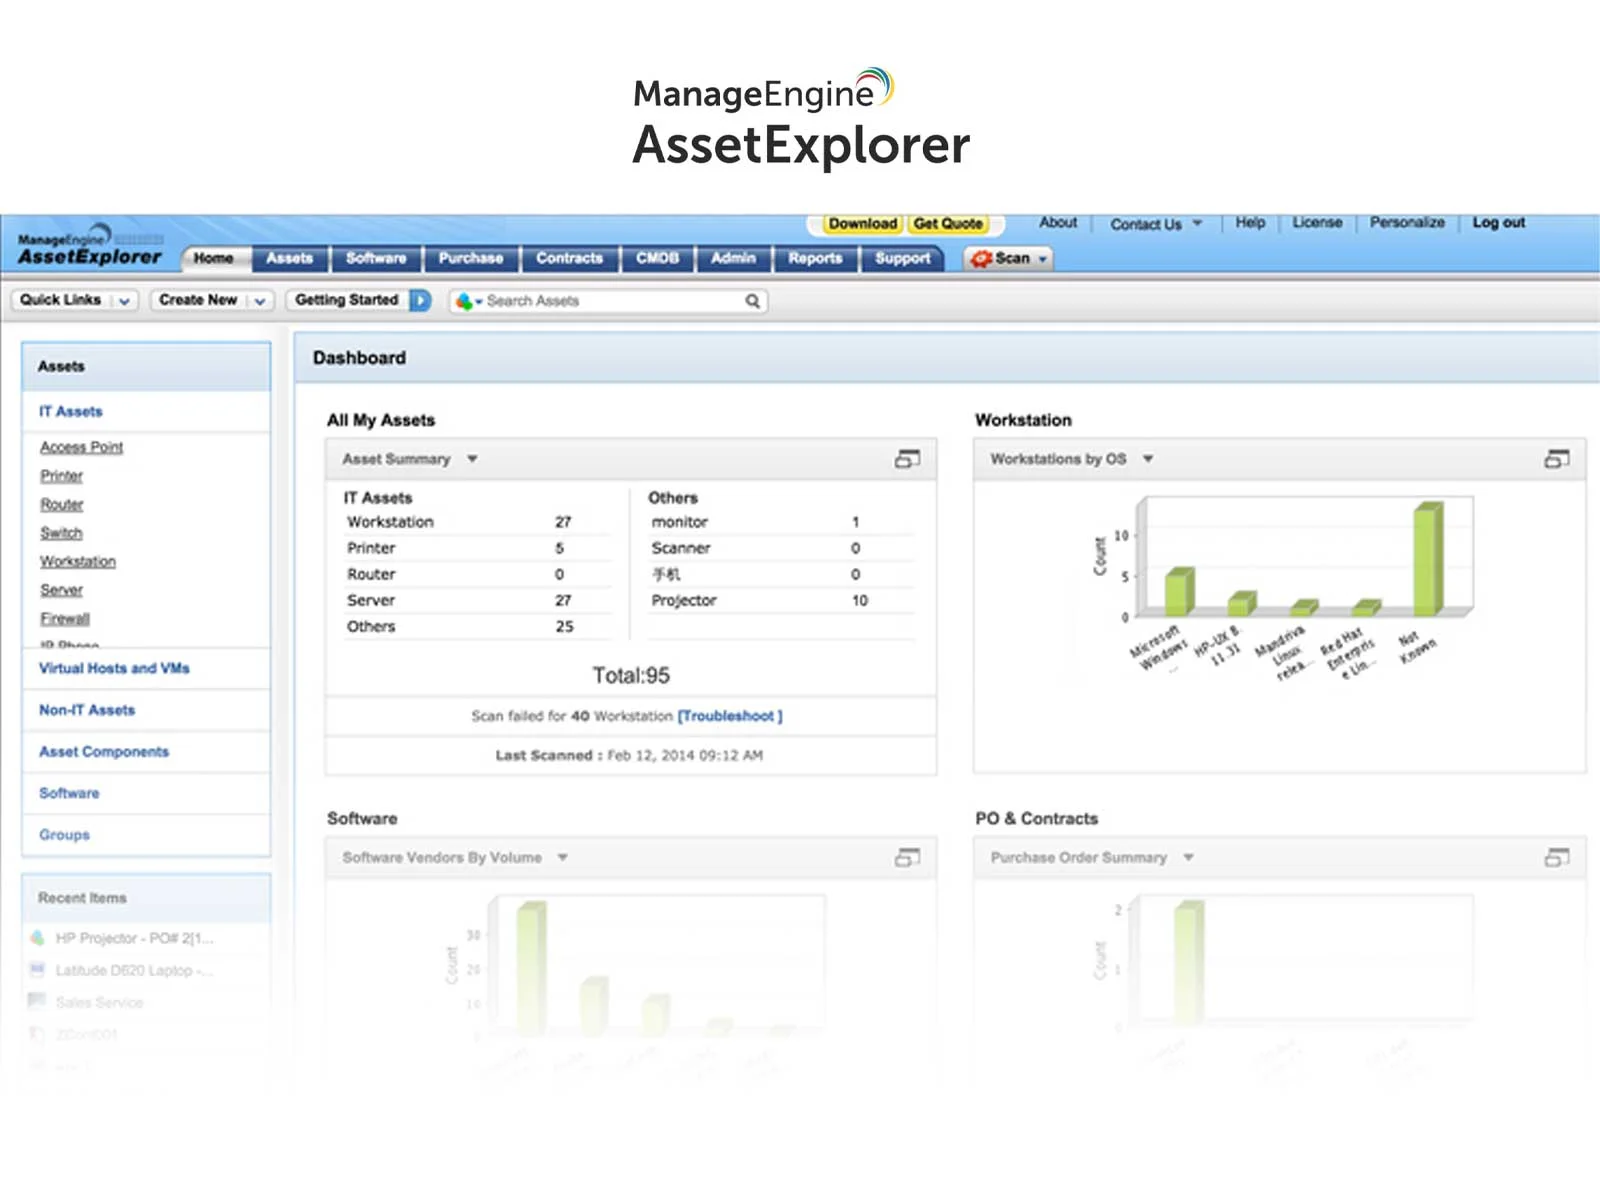
\includegraphics[width=\linewidth]{Images/C3/ManageEngine.png}
%     \caption{ManageEngine Asset Explorer\\ Nguồn: manageengine.com, truy cập vào ngày 01/05/2025}
% \end{figure}

% \noindent \textbf{Các chức năng chính}
% \begin{itemize}[label=--]
%     \item Quản lý kho lưu trữ phần mềm và phần cứng
%     \item Phát hiện và giám sát tài sản
%     \item Ánh xạ và quản lý cấu hình (CMDB)
%     \item Quản lý hợp đồng và giấy phép
%     \item Báo cáo và phân tích
%     \item Quản lý thời hạn dịch vụ và bảo dưỡng
%     \item Lập kế hoạch mua sắm tài sản
%     \item Theo dõi tuân thủ sử dụng
% \end{itemize}
% \textbf{Ưu điểm}
% \begin{itemize}[label=--]
%     \item Quản lý tài sản toàn diện: Asset Explorer không chỉ giúp quản lý tài sản phần cứng và phần mềm mà còn cung cấp nhiều chức năng như quản lý hợp đồng, giấy phép và theo dõi thời hạn bảo dưỡng.
%     \item Ứng dụng di động: Hỗ trợ quản lý tài sản từ xa, tăng tính linh hoạt.
%     \item Quản lý cấu hình dễ dàng: Cơ sở dữ liệu quản lý cấu hình (CMDB) giúp dễ dàng cấu hình và giám sát tài sản mạng để đảm bảo hiệu suất tối ưu.
% \end{itemize}
% \textbf{Nhược điểm}
% \begin{itemize}[label=--]
%     \item Chi phí cho tính năng truy cập từ xa cao: Add-on truy cập từ xa có thể gây khó khăn cho người dùng có ngân sách hạn chế.
%     \item Độ khó cho người mới: Giao diện và tính năng có thể gây khó khăn cho người mới sử dụng.
% \end{itemize}
% \subsection{ServiceNow IT Asset Management}
% \noindent \textbf{ServiceNow IT Asset Management} \cite{servicenow} là một phần của nền tảng ServiceNow, được ra mắt vào năm 2017. Gói dịch vụ này bao gồm mô-đun CMDB cũng như mô-đun SAM đều tương đối mới. Cho phép người dùng quản lý các bản quyền phần mềm, tài sản phần cứng và khả năng theo dõi vòng đời tài sản. Gói dịch vụ này cung cấp cho cả người dùng không sử dụng gói dịch vụ ITSM (quản lý dịch vụ công nghệ thông tin) của ServiceNow.
% \begin{figure}[H]
%     \centering
%     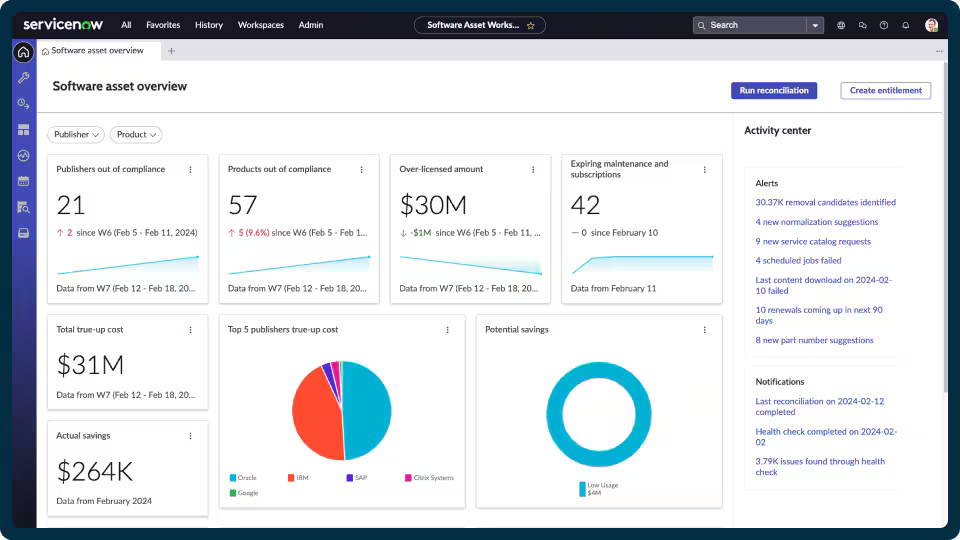
\includegraphics[width=0.8\linewidth]{Images/C3/ServiceNow.png}
%     \vspace{10pt}
%     \caption{ServiceNow IT Asset Management\\ Nguồn: servicenow.com, truy cập vào ngày 01/05/2025}
% \end{figure}

% \noindent \textbf{Các chức năng chính}  
% \begin{itemize}[label=--]
%     \item Quản lý kho lưu trữ phần mềm và phần cứng
%     \item Phát hiện và giám sát tài sản 
%     \item Quản lý tài nguyên đám mây
%     \item Báo cáo và phân tích
%     \item Đăng xuất tài sản CNTT (IT Asset Offboarding)
%     \item Quản lý giấy phép SaaS (Software as a Service)
% \end{itemize}
% \textbf{Ưu điểm}
% \begin{itemize}[label=--]
%     \item Quản lý tài sản tập trung: Tất cả thông tin về tài sản và vòng đời của nó được lưu trữ trong một hệ thống duy nhất.
%     \item Hỗ trợ tích hợp: Có khả năng cập nhật thông tin từ các công cụ khác như AirWatch, SentinelOne.
%     \item Theo dõi và gia hạn giấy phép: Đảm bảo tuân thủ và tránh vi phạm giấy phép.
%     \item Giao diện thân thiện: Hệ thống không chỉ có giao diện thân thiện với người dùng, đảm bảo dễ triển khai mà còn hỗ trợ khách hàng rất tốt, giúp quá trình triển khai trở nên mượt mà.
% \end{itemize}
% \textbf{Nhược điểm}
% \begin{itemize}[label=--]
%     \item Chi phí cao cho doanh nghiệp nhỏ: Phần mềm có thể quá đắt đối với các doanh nghiệp nhỏ.
%     \item Phân quyền phức tạp: Quá trình phân quyền người dùng yêu cầu nhiều bước, dễ gây nhầm lẫn.
%     \item Báo cáo phức tạp: Quá nhiều tùy chọn trong việc tạo báo cáo, đôi khi khiến người dùng khó sử dụng hiệu quả.
%     \item Hiệu suất thấp: Vì có rất nhiều tính năng nên cần dùng nhiều tài nguyên để vận hành, đôi khi hệ thống sẽ phản hồi chậm, làm giảm hiệu  suất.
% \end{itemize}
% \subsection{InvGate Insight}
% \noindent \textbf{InvGate Insight}\cite{invgate} cung cấp cho khách hàng các công cụ để tạo một kho lưu trữ thống nhất cho tất cả tài sản CNTT được kết nối với mạng (bao gồm tài sản ảo, vật lý và trên đám mây) trên cùng một nền tảng. Được nhắm đến các tổ chức vừa và lớn nhưng cũng phù hợp với các công ty nhỏ hơn, Insight cung cấp cái nhìn toàn diện về toàn bộ hệ thống CNTT với cấu hình dễ dàng bằng No-Code/Low-Code mà không cần tích hợp đắt tiền – giảm đáng kể Tổng Chi Phí Sở Hữu (TCO). 
% \begin{figure}[H]
%     \centering
%     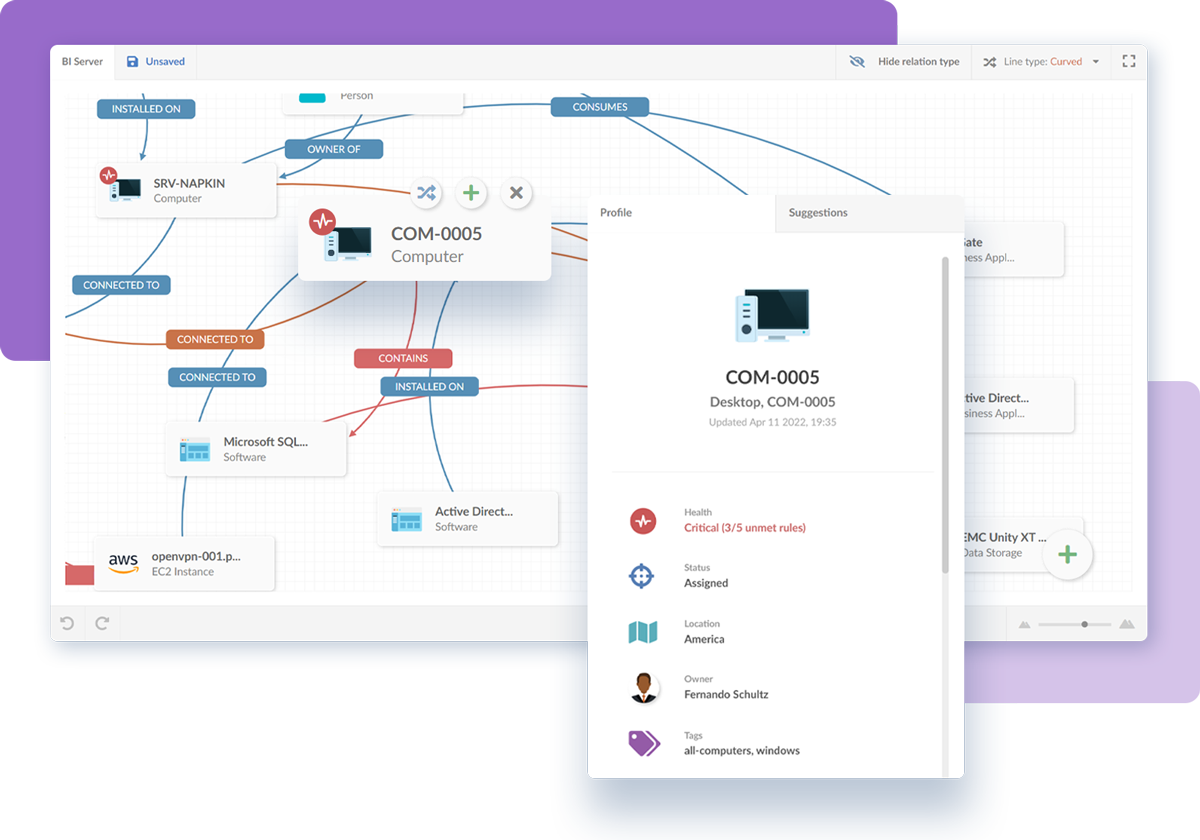
\includegraphics[width=\linewidth]{Images/C3/InvGate_Insight.png}
%     \caption{InvGate Insight\\ Nguồn: invgate.com, truy cập vào ngày 01/05/2025}
% \end{figure}

% \noindent \textbf{Các tính năng chính}
% \begin{itemize}[label=--]
%     \item Quản lý kho lưu trữ phần mềm và phần cứng
%     \item Tự động hóa các quy trình quản lý tài sản
%     \item Cơ sở dữ liệu quản lý cấu hình (CMDB)
%     \item Quản lý tuân thủ an ninh CNTT
%     \item Phát hiện và giám sát tài sản
%     \item Đo lường phần mềm
%     \item Điều khiển từ xa
%     \item Quản lý tài chính CNTT
% \end{itemize}
% \textbf{Ưu điểm}
% \begin{itemize}[label=--]
%     \item Tối ưu hóa cho việc quản lý giấy phép và hợp đồng.
%     \item Được thiết kế để hoạt động liền mách với InvGate Service Desk.
%     \item Tối ưu hóa để giúp tổ chức giảm chi phí, quản lý tuân thủ và rủi ro hiệu quả hơn, cũng như hỗ trợ ra quyết định tốt hơn.
% \end{itemize}
% \textbf{Nhược điểm}
% \begin{itemize}[label=--]
%     \item Hạn chế trong tùy chỉnh: Mặc dù hỗ trợ No-Code/Low-Code, một số chức năng phức tạp hơn vẫn có thể yêu cầu kiến thức kỹ thuật hoặc hỗ trợ từ đội ngũ chuyên gia.
%     \item Không phù hợp với môi trường phi mạng: Giải pháp này tập trung vào tài sản kết nối mạng, do đó có thể không hỗ trợ tốt cho những tổ chức có nhiều tài sản CNTT không được kết nối mạng.
%     \item Chi phí triển khai: Dù không cần tích hợp phức tạp, chi phí cấp phép và duy trì cho các tổ chức nhỏ hoặc rất nhỏ có thể vẫn khá cao.
%     \item Giới hạn tính năng tích hợp bên thứ ba: Có thể không tích hợp tốt với tất cả các công cụ hoặc nền tảng khác mà tổ chức đang sử dụng.
% \end{itemize}
% \subsection{Asset Panda}
% \noindent \textbf{Asset Panda} \cite{assetpanda} là một nền tảng theo dõi tài sản dựa trên đám mây, linh hoạt đáp ứng nhu cầu Quản lý Tài sản cụ thể, chủ yếu hướng đến các doanh nghiệp vừa và nhỏ.
% \begin{figure}[H]
%     \centering
%     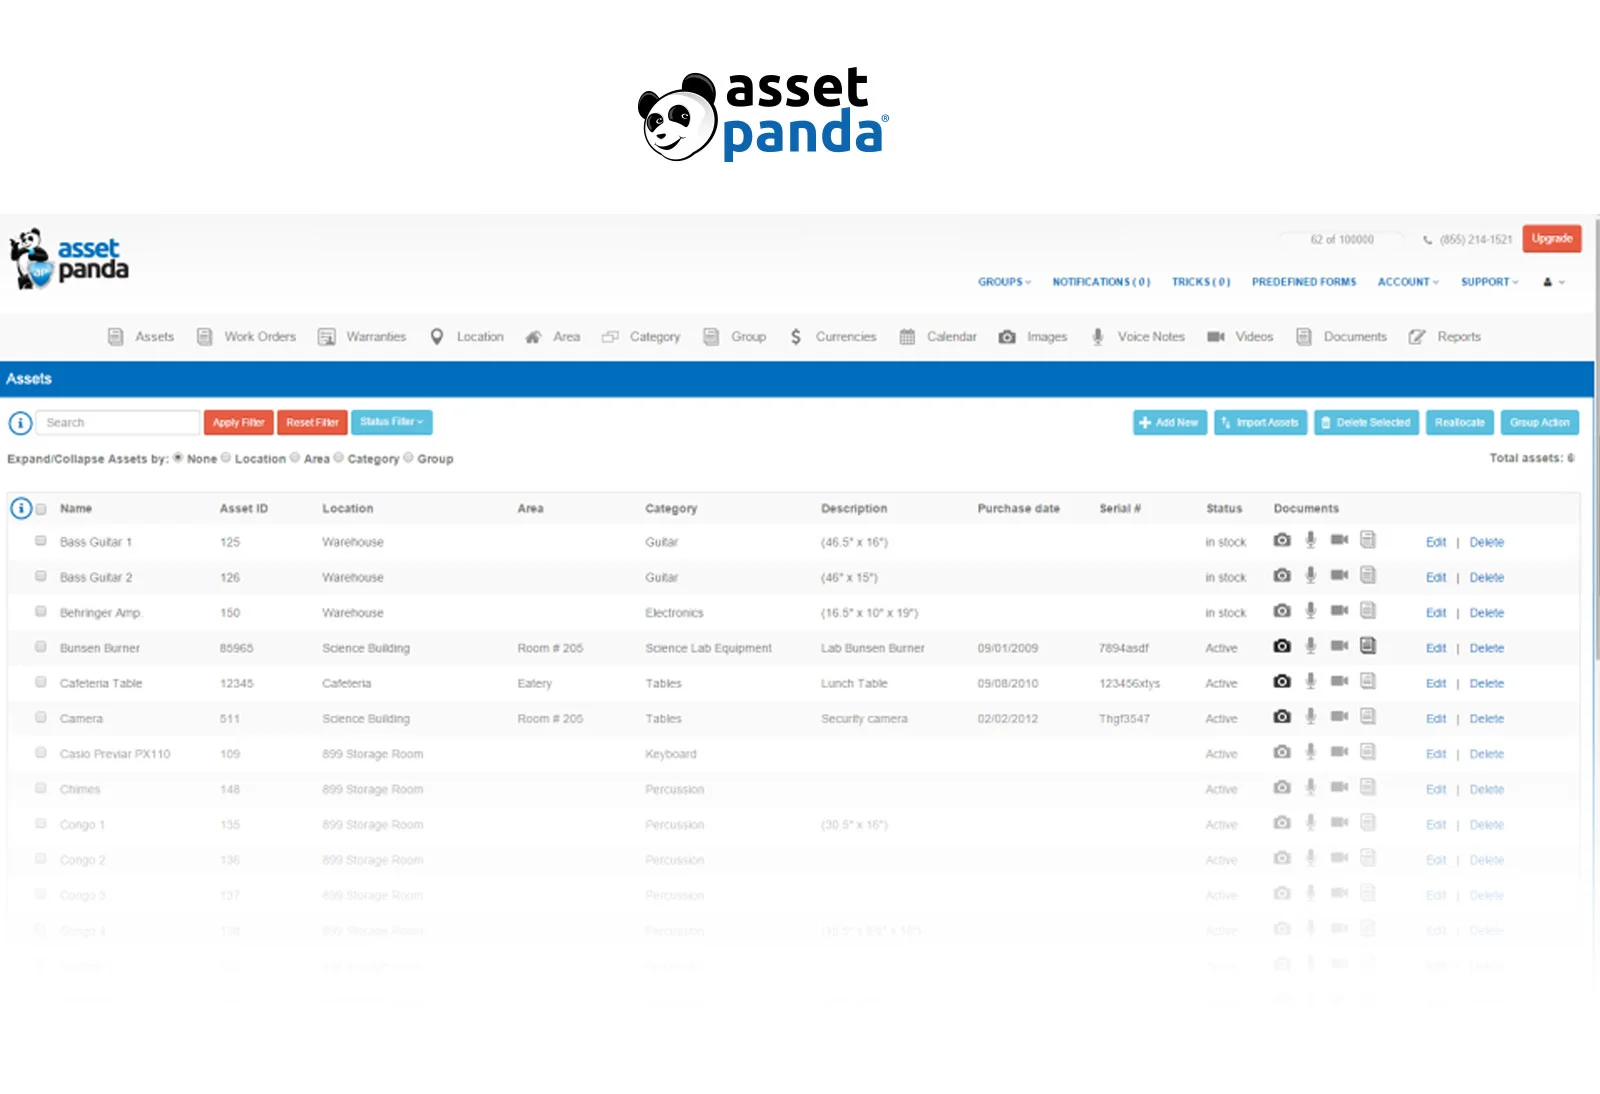
\includegraphics[width=\linewidth]{Images/C3/Asset_Panda.png}
%     \caption{Asset Panda\\ Nguồn: assetpanda.com, truy cập vào ngày 01/05/2025}
% \end{figure}

% \noindent \textbf{Các chức năng chính}
% \begin{itemize}[label=--]
%     \item Ứng dụng di động để cập nhật và theo dõi dữ liệu tài sản CNTT
%     \item Cảnh báo và thông báo về yêu cầu sửa chữa và các sự kiện khác
%     \item Theo dõi toàn bộ vòng đời của tài sản
% \end{itemize}
% \textbf{Ưu điểm}
% \begin{itemize}[label=--]
%     \item Giao diện đơn giản và dễ sử dụng.
%     \item Thông báo và cảnh báo sự kiện tài sản kịp thời.
% \end{itemize}
% \textbf{Nhược điểm}
% \begin{itemize}[label=--]
%     \item Không có chức năng đăng ký người dùng: Điều này có thể gây bất tiện cho việc quản lý người dùng trong hệ thống.
%     \item Không có khả năng theo dõi phần mềm đã cài đặt: Điều này hạn chế việc kiểm soát phần mềm trên các tài sản CNTT.
%     \item Không hỗ trợ phát hiện tài sản theo thời gian thực: Điều này có thể gây khó khăn trong việc theo dõi các tài sản mới hoặc đã thay đổi.
%     \item Báo cáo hạn chế tùy chỉnh.
%     \item Hỗ trợ khách hàng không ổn định.
% \end{itemize} 

% \subsection{Nhận xét chung}
% \noindent Các ứng dụng quản lý tài sản công nghệ thông tin được trình bày bên trên đều có những ưu điểm và nhược điểm riêng \cite{topitam}. Dưới đây là bảng thống kê các tính năng của chúng:
% \begin{table}[h!]
%     \centering
%     \caption{So sánh tính năng giữa các công cụ quản lý tài sản IT}
%     \begin{tabular}{|p{4cm}|p{2.5cm}|p{2.5cm}|p{2.5cm}|p{2.5cm}|}
%         \hline
%         Tính năng & ManageEngine & ServiceNow & InvGate Insight & Asset Panda \\
%         \hline
%         Phát hiện và giám sát tài sản & Có & Có & Có & Có \\
%         \hline
%         Quản lý vòng đời tài sản (Asset Lifecycle) & Có & Có & Có & Có \\
%         \hline
%         Quản lý kho phần cứng và phần mềm & Có & Có & Có & Có \\
%         \hline
%         Báo cáo và phân tích & Có & Có & Có & Có \\
%         \hline
%         Quản lý cấu hình (CMDB) & Có & Có & Có & Có \\
%         \hline
%         Truy cập di động & Add-on & Có & Không & Có \\
%         \hline
%         Tự động phát hiện tài sản & Có & Có & Có & Không \\
%         \hline
%         Tích hợp với hệ thống ITSM & Hạn chế & Toàn diện & Tích hợp liền mạch với InvGate Service Desk & Không \\
%         \hline
%         Quản lý tài nguyên đám mây & Không & Có & Không & Không \\
%         \hline
%         Điều khiển từ xa (Remote Desktop) & Add-on & Có & Có & Không \\
%         \hline
%         Đo lường phần mềm (Software Metering) & Không & Có & Có & Không \\
%         \hline
%         Quản lý tài chính IT & Có & Có & Có & Không \\
%         \hline
%         Quản lý rủi ro và an ninh IT & Có & Có & Có & Không \\
%         \hline
%         Cấu hình No-code/Low-code & Không & Không & Có & Không \\
%         \hline
%         Quản lý giấy phép SaaS & Không & Có & Không & Không \\
%         \hline
%         Giám sát tài sản theo thời gian thực & Có & Có & Có & Không\\
%         \hline
%         Hosting & Đám mây, tại chỗ (Cloud \& On-premise) & Đám mây & Đám mây, tại chỗ (Cloud \& On-premise) & Đám mây\\
%         \hline
%         Thời gian dùng thử & 30 ngày & Không & 30 ngày & 14 ngày\\
%         \hline
%         Chi phí & Bắt đầu từ \$955/năm cho 250 tài sản, lên tới \$11,995/năm cho 10,000 tài sản & Yêu cầu báo giá (Request a quote) & Yêu cầu báo giá (Request a quote) & \$1,500 mỗi năm cho tối đa 500 tài sản\\
%         \hline
%         Chi phí tích hợp & Yêu cầu báo giá & Yêu cầu báo giá & API miễn phí và tích hợp nội bộ & Yêu cầu báo giá \\
%         \hline
%     \end{tabular}    
    
%     \label{table:comparison}
% \end{table}
% \vspace{1em}
% \begin{itemize}[label=--]
%     \item ManageEngine Asset Explorer nổi bật với khả năng quản lý toàn diện tài sản phần cứng và phần mềm, kèm theo tính năng quản lý hợp đồng và giám sát tuân thủ. Tuy nhiên, không hỗ trợ quản lý tài nguyên đám mây và các tính năng nâng cao như SaaS License Management.
%     \item ServiceNow IT Asset Management phù hợp với các tổ chức lớn nhờ tích hợp đầy đủ với ITSM, quản lý tài nguyên đám mây, và quản lý giấy phép SaaS, giúp theo dõi và đảm bảo tuân thủ giấy phép phần mềm.
%     \item InvGate Insight nổi bật với tính năng cấu hình No-code/Low-code và tích hợp chặt chẽ với InvGate Service Desk. Đây là lựa chọn tối ưu cho các tổ chức muốn tùy biến mà không cần chi phí tích hợp cao.
%     \item Asset Panda tập trung vào việc theo dõi tài sản qua di động, nhưng thiếu các tính năng nâng cao như giám sát thời gian thực và quản lý phần mềm SaaS.
% \end{itemize}
% \subsection{Kết chương}
% \noindent Tùy thuộc vào ngân sách, quy mô và yêu cầu cụ thể, sự lựa chọn giữa các hệ thống này này phụ thuộc vào ưu tiên cụ thể của người sử dụng. Nhưng nhìn chung, các hệ thống trên đều có giá rất cao cũng như số lượng dùng thử hạn chế. Thêm vào đó mỗi hệ thống sẽ có một thiên hướng cụ thể về phát hiện hay quản lý tài sản. Ví dụ như Asset Panda tập trung mạnh vào việc quản lý tài sản hay InvGate Insight nổi bật với việc kết hợp phát hiện tài sản mạnh mẽ và phân tích trực quan để giúp đưa ra quyết định quản lý tài sản hiệu quả hơn. Vì lý do như thế, nhóm sẽ hiện thực lại một hệ thống phát hiện và quản lý tài sản CNTT tích hợp cả hai chức năng với giá thành thấp hơn. Quan trọng hơn hết, nhóm tập trung vào tính năng giám sát tài sản thời gian thực.


%  \newpage
% \section{Thực nghiệm}
%%%%%%%%%%%%%%%%%%%%%%%%%%%%%%%%%
\subsection{Mục tiêu thực nghiệm}
Mục tiêu của giai đoạn thực nghiệm đầu tiên là kiểm chứng tính khả thi của \textit{kiến trúc giám sát lai} trong bài toán phát hiện và thẩm định bất thường trên môi trường \textit{server/cloud}. Cụ thể, thực nghiệm tập trung đánh giá việc kết hợp giữa mô hình phát hiện bất thường trên dữ liệu metric, cơ chế truy xuất ngữ cảnh từ \textit{log/trace} và \textit{LLM-as-a-Judge} trong quy trình xử lý cảnh báo.

Các mục tiêu chính của giai đoạn này bao gồm:
\begin{itemize}[label=--]
    \item \textbf{Kiểm chứng khả năng vận hành end-to-end của pipeline giám sát lai.}\\
Thực nghiệm cần xác minh rằng dữ liệu thô có thể được xử lý qua đầy đủ các bước: chuẩn hóa dữ liệu, tạo cửa sổ metric, phát hiện bất thường, tạo cảnh báo ứng viên, truy xuất ngữ cảnh liên quan, xây dựng prompt, gọi LLM-as-a-Judge, đưa ra quyết định cuối cùng và ghi nhận kết quả đánh giá.
    \item \textbf{Đánh giá vai trò của mô hình phát hiện bất thường trên metric.}\\
Mô hình phát hiện sơ cấp được sử dụng để quét dữ liệu metric và xác định các cửa sổ có dấu hiệu bất thường. Mục tiêu là đánh giá khả năng của tầng này trong việc phát hiện các ứng viên bất thường ban đầu, đồng thời xác định những trường hợp mà việc chỉ dựa trên metric có thể dẫn đến cảnh báo sai hoặc bỏ sót bất thường.
    \item \textbf{Đánh giá tác động của ngữ cảnh log/trace đối với quá trình thẩm định cảnh báo.}\\
Thực nghiệm kiểm tra liệu việc bổ sung log và trace liên quan có giúp LLM đưa ra quyết định chính xác hơn so với khi chỉ sử dụng thông tin metric hay không. Đây là mục tiêu quan trọng nhằm kiểm chứng giả thuyết rằng ngữ cảnh vận hành có thể hỗ trợ phân biệt giữa cảnh báo thật và cảnh báo giả.
    \item \textbf{Đánh giá vai trò của LLM-as-a-Judge trong việc phân loại cảnh báo.}\\
LLM không được sử dụng như bộ phát hiện bất thường chính, mà đóng vai trò thẩm định các cảnh báo ứng viên đã được mô hình sơ cấp phát hiện. Thực nghiệm cần đánh giá khả năng của LLM trong việc đưa ra nhãn như cảnh báo thật, cảnh báo giả hoặc trường hợp chưa đủ chắc chắn, dựa trên metric snapshot và ngữ cảnh được truy xuất.
    \item \textbf{So sánh các biến thể thực nghiệm để xác định đóng góp của từng thành phần.}\\
Các biến thể như \textbf{detector-only}, \textbf{LLM without RAG} và\textbf{ hybrid RAG + LLM} được sử dụng để phân tích sự khác biệt giữa việc chỉ dùng metric, dùng LLM không có ngữ cảnh, và dùng LLM có bổ sung log/trace context. Qua đó, thực nghiệm làm rõ vai trò của từng thành phần trong pipeline.
    \item \textbf{Đo lường các chỉ số đánh giá cốt lõi của hệ thống.}\\
Các chỉ số được sử dụng bao gồm Precision, Recall, F1-score, False Positive Rate, tỷ lệ giảm cảnh báo giả, số lần gọi LLM, độ trễ xử lý, tỷ lệ JSON hợp lệ và các thông tin liên quan đến token/cost. Những chỉ số này giúp đánh giá không chỉ chất lượng phân loại, mà còn khả năng vận hành của kiến trúc trong điều kiện thí nghiệm.
    \item  \textbf{Xác định các giới hạn ban đầu của kiến trúc}\\
Bên cạnh việc đo lường hiệu quả, thực nghiệm cũng nhằm phát hiện các điểm còn hạn chế như trường hợp detector bỏ sót bất thường, chất lượng truy xuất ngữ cảnh chưa ổn định, hoặc LLM cần thêm thông tin để đưa ra quyết định chắc chắn. Các giới hạn này sẽ là cơ sở cho những cải tiến ở các giai đoạn tiếp theo của đề tài.
\end{itemize}
Tóm lại, giai đoạn thực nghiệm đầu tiên tập trung trả lời câu hỏi: kiến trúc kết hợp giữa \textbf{detector},\textbf{ RAG} và\textbf{ LLM-as-a-Judge} có thể hỗ trợ thẩm định cảnh báo bất thường hiệu quả hơn so với cách tiếp cận chỉ dựa trên metric hay không. Kết quả của giai đoạn này sẽ được dùng làm cơ sở để phân tích tính khả thi, điểm mạnh và điểm yếu của kiến trúc giám sát lai trong môi trường \textit{server/cloud}.
\subsection{Dữ liệu thực nghiệm}
Trong giai đoạn thực nghiệm đầu tiên, nghiên cứu sử dụng hai bộ dữ liệu chính: Microsoft Cloud Monitoring và Nezha. Hai bộ dữ liệu này được lựa chọn nhằm phản ánh các khía cạnh đa chiều của bài toán giám sát hiệu năng hệ thống. Việc sử dụng đồng thời hai bộ dữ liệu cho phép đánh giá độc lập và toàn diện từng thành phần của kiến trúc đề xuất, từ tầng phát hiện bất thường trên chuỗi thời gian đến kiến trúc giám sát lai.
\begin{table}[H]
    \centering
    \renewcommand{\arraystretch}{1.6} % Tăng khoảng cách dòng cho thoáng, giống trong ảnh
    \begin{tabularx}{\textwidth}{
        >{\raggedright\arraybackslash}p{3.5cm} % Cột 1 độ rộng cố định
        >{\raggedright\arraybackslash}X      % Cột 2 tự động giãn
        >{\raggedright\arraybackslash}X      % Cột 3 tự động giãn
    }
        \toprule
        \rowcolor{blue!5} % Thêm màu nền xanh xám nhạt cho hàng tiêu đề
        \textbf{Bộ dữ liệu} & \textbf{Đặc điểm chính} & \textbf{Vai trò trong thực nghiệm} \\
        \midrule
        
        \textbf{Microsoft Cloud Monitoring} & 
        Cung cấp chuỗi thời gian metric có nhãn bất thường  trên từng điểm dữ liệu. & 
        Kiểm thử mô hình cơ sở, đánh giá điểm bất thường và tạo cảnh báo ứng viên. \\
        
        \textbf{Nezha Dataset} & 
        Dữ liệu đa nguồn gồm metric, log, trace, trace ID và danh sách mô phỏng lỗi. & 
        Đánh giá toàn bộ chuỗi quy trình trong việc thẩm định cảnh báo. \\
        
        \bottomrule
    \end{tabularx}
    \caption{Tóm tắt đặc điểm và vai trò của các bộ dữ liệu}
    \label{tab:dataset_summary}
\end{table}
\subsubsection{Microsoft Cloud Monitoring Dataset}
Bộ dữ liệu \textbf{Microsoft Cloud Monitoring} bao gồm các chuỗi thời gian metric hiệu năng được thu thập trong bối cảnh giám sát dịch vụ đám mây. Dữ liệu thô gồm các tệp CSV chứa điểm dữ liệu và metadata tương ứng. Với nhãn trạng thái (bình thường hoặc bất thường) được gán cụ thể, bộ dữ liệu này đặc biệt phù hợp để đánh giá và tinh chỉnh ngưỡng cho các mô hình phát hiện bất thường trên chuỗi dữ liệu \textbf{metric}.  

Sau quá trình tiền xử lý, dữ liệu bao gồm 60 chuỗi thời gian với 225.403 điểm dữ liệu hợp lệ, được thu thập từ ngày 01/11/2017 đến ngày 18/07/2018 (UTC). Số lượng điểm bất thường ghi nhận là 4.553, chiếm tỷ lệ khoảng 2,02\%. Tập dữ liệu này bao phủ nhiều miền ứng dụng đa dạng như \textit{tỷ lệ lỗi ứng dụng} (application crash rate), \textit{độ trễ phụ thuộc} hay \textit{tỷ lệ yêu cầu API}. Mức độ phân bố bất thường không đồng đều giữa các miền; ví dụ, nhóm application-crash-rate-1 có tỷ lệ lỗi cao đáng kể, trong khi nhóm service-unavailable không ghi nhận điểm bất thường nào. 

Trong phạm vi đề tài, bộ dữ liệu này đóng vai trò phụ trợ nhằm kiểm chứng khả năng sinh cảnh báo ứng viên của tầng nhận diện cơ sở trước khi kết quả được chuyển giao cho LLM xử lý.
\subsubsection{Nezha Dataset}
\textbf{Nezha} là bộ dữ liệu thực nghiệm chính, được xây dựng cho hệ thống phân tích microservice. Ưu điểm nổi bật của Nezha là cung cấp không gian quan sát đa chiều bao gồm: metric, log, trace, và các sự kiện lỗi được chủ động tiêm vào hệ thống (fault injection). Sự đa dạng về dữ liệu vận hành này là điều kiện tiên quyết để kiểm chứng năng lực của hệ thống RAG và LLM-as-a-Judge.  

Dữ liệu \textbf{Nezha} được phân vùng theo các ngày từ tháng 08/2022 đến tháng 01/2023, ghi nhận 101 sự kiện fault injection thuộc 5 nhóm chính: network\_delay (30 sự kiện), cpu\_contention (23 sự kiện), exception (20 sự kiện), return (18 sự kiện) và cpu\_consumed (10 sự kiện). Về đo lường hiệu năng, tập dữ liệu thô chứa 112 tệp với 95.660 dòng metric, bao trùm 56 service và 103 pod. Đặc điểm nổi bật của tập dữ liệu này là tính mất cân bằng cực kỳ cao: chỉ có 527 dòng metric (tương đương 0,55\%) nằm trong các khung thời gian xảy ra lỗi (fault window).  

Sau khi tiền xử lý, dữ liệu được chuẩn hóa thành hai tài nguyên (artifact) chính phục vụ chuỗi quy trình:
\begin{itemize}[label=--]
    \item Tệp \textbf{metrics.csv}: Chứa 95.660 dòng dữ liệu theo dõi hiệu năng (CPU, memory, network, latency...). Dữ liệu này đóng vai trò đầu vào cho bước tạo cửa sổ trượt và nhận diện bất thường, trong đó chứa 527 cảnh báo thực (true\_alert).
    \item Tệp \textbf{logs.jsonl}: Chứa 11.696 sự kiện ngữ cảnh (gồm 5.921 application log và 5.775 trace span). Phần lớn dữ liệu mang nhãn mức độ INFO (11.544 bản ghi), số ít còn lại thuộc nhóm \textit{WARN}, \textit{ERROR} và \textit{WARNING}. Tệp này hoạt động như một nguồn cơ sở tri thức để hệ thống RAG truy xuất ngữ cảnh cho từng cảnh báo ứng viên.  
\end{itemize}
Nhãn true\_alert được gán dựa trên thông tin fault injection của cùng một pod trong khoảng thời gian từ 60 giây trước đến 360 giây sau khi xảy ra lỗi. Cơ chế này giúp thu hẹp phạm vi ngữ cảnh truy xuất từ log/trace, tránh tình trạng quá tải thông tin khi đưa vào prompt cho mô hình ngôn ngữ.  
\subsection{Môi trường và thiết lập thực nghiệm}
Môi trường thực nghiệm được xây dựng nhằm kiểm chứng tính khả thi của kiến trúc giám sát lai trong bài toán mô hình ngôn ngữ lớn trong thời gian thực. Đặc biệt, hệ thống được thiết kế để xử lý dòng dữ liệu thu thập từ đa dạng môi trường, bao gồm cả máy chủ (server/cloud) lẫn các thiết bị đầu cuối (desktop, laptop). Ở giai đoạn này, mô hình chưa hướng đến việc triển khai như một nền tảng hoàn chỉnh, mà tập trung xác thực một chuỗi quy trình xử lý: từ dữ liệu thô đầu vào đến quyết định thẩm định cuối cùng.

\subsubsection{Kiến trúc giám sát lai}
\begin{figure}[H]
    \centering
    \resizebox{0.95\textwidth}{!}{
    \begin{tikzpicture}[
        node distance=0.8cm and 1.0cm,
        box/.style={
            rectangle,
            draw,
            rounded corners,
            align=center,
            minimum width=3.0cm,
            minimum height=1.0cm,
            font=\small\bfseries,
            fill=blue!5, % Màu nền xanh nhạt giúp sơ đồ hiện đại hơn
            thick
        },
        arrow/.style={-{Stealth}, thick}
    ]

        % Hàng 1: Từ trái sang phải
        \node[box] (metric) {Metric thô};
        \node[box, right=of metric] (preproc) {Tiền xử lý};
        \node[box, right=of preproc] (detector) {Mô hình nhận diện\\(Detector)};
        \node[box, right=of detector] (alert) {Cảnh báo\\ứng viên};

        % Hàng 2: Từ phải sang trái (bên dưới Alert)
        \node[box, below=1.2cm of alert] (gate) {Cổng phân luồng\\(LLM Gate)};
        \node[box, left=of gate] (rag) {Truy xuất RAG};
        \node[box, left=of rag] (llm) {LLM-as-a-Judge};
        \node[box, left=of llm] (decision) {Quyết định \&\\Dự phòng};

        % Hàng 3: Khúc cuối (bên dưới Decision)
        \node[box, below=1.2cm of decision] (eval) {Đánh giá \&\\Lưu vết};

        % Vẽ mũi tên
        \draw[arrow] (metric) -- (preproc);
        \draw[arrow] (preproc) -- (detector);
        \draw[arrow] (detector) -- (alert);
        
        % Mũi tên uốn từ Hàng 1 xuống Hàng 2
        \draw[arrow] (alert) -- (gate);
        
        \draw[arrow] (gate) -- (rag);
        \draw[arrow] (rag) -- (llm);
        \draw[arrow] (llm) -- (decision);
        
        % Mũi tên uốn từ Hàng 2 xuống Hàng 3
        \draw[arrow] (decision) -- (eval);

    \end{tikzpicture}
    }
    \vspace{0.5cm}
    \caption{Kiến trúc luồng xử lý của hệ thống giám sát lai}
    \label{fig:hybrid-pipeline}
\end{figure}

Đầu vào của pipeline là dữ liệu \textit{metric} và \textit{log/trace} đã được chuẩn hóa. Dữ liệu metric đi qua tầng tiền xử lý để chuẩn hóa mốc thời gian và trích xuất thành các cửa sổ trượt . Mỗi cửa sổ đại diện cho một khung thời gian vận hành và được đưa vào Mô hình nhận diện. Nếu phát hiện dấu hiệu bất thường về tài nguyên hoặc hiệu năng, hệ thống sẽ sinh ra một "ứng viên cảnh báo".

Để tối ưu hóa chi phí và độ trễ, cảnh báo không được gửi trực tiếp đến LLM. Thay vào đó, Cổng phân luồng (LLM Gate) sẽ sàng lọc các cảnh báo đủ điều kiện. Các cảnh báo vượt qua vòng lặp này sẽ kích hoạt cơ chế RAG để truy xuất ngữ cảnh vận hành liên quan. Bộ tổng hợp sau đó sẽ định dạng dữ liệu metric và ngữ cảnh thành câu lệnh cấu trúc, giao cho LLM thẩm định xem đây là cảnh báo thật, cảnh báo giả, hay trạng thái không chắc chắn. Kết quả cuối cùng được đánh giá và lưu vết tự động.

Do đó, LLM không đóng vai trò phát hiện bất thường sơ cấp. Việc phát hiện được giao cho các detector truyền thống để đảm bảo tốc độ trên dòng dữ liệu thời gian thực, trong khi LLM chỉ tham gia ở tầng hậu kỳ nhằm khai thác năng lực suy luận ngữ cảnh sâu sắc đối với các ca khó.

\subsubsection{Các thành phần chính}
\begin{itemize}[label=--]
    \item \textbf{Tiền xử lý dữ liệu:} Thành phần này chuẩn bị dữ liệu đầu vào thông qua các bước: đồng bộ mốc thời gian, chuẩn hóa giá trị và áp dụng kỹ thuật cửa sổ trượt. Cơ chế cửa sổ trượt giúp chuyển đổi luồng dữ liệu liên tục thành các khối dữ liệu hữu hạn, cho phép hệ thống liên tục đánh giá trạng thái gần nhất của thiết bị hoặc dịch vụ.
    \item \textbf{Mô hình nhận diện sơ cấp:} Đóng vai trò là bộ lọc đầu tiên, nhận diện các sai lệch phân bố. Hệ thống thực nghiệm hiện tại hỗ trợ hai thuật toán chính:
    \begin{itemize}
        \item \textbf{FeaturePressureDetector}: Mô hình tinh gọn, ít phụ thuộc thư viện, đánh giá nhanh áp lực tài nguyên phần cứng.

        \item \textbf{IsolationForestDetecto}r: Mô hình học máy dưạ trên thuật toán Isolation Forest của \textit{scikit-learn}, có khả năng học phân bố dữ liệu bình thường và cô lập các chuỗi hành vi dị thường.
    \end{itemize}
    \item \textbf{Cảnh báo ứng viên:} Là đối tượng dữ liệu trung gian mang tính chuẩn hóa, được sinh ra khi detector phát hiện bất thường. Một payload ứng viên tiêu chuẩn bao gồm: alert\_id, time\_window, node\_id, service\_id, metric\_snapshot, anomaly\_score, và top\_features. Việc chuẩn hóa này đảm bảo tính nhất quán định dạng cho toàn bộ các khâu xử lý ngữ cảnh và lưu vết phía sau.
    \item \textbf{Cổng phân luồng (LLM Gate)}: Thành phần này kiểm soát lưu lượng truy vấn LLM thông qua các chính sách: ngưỡng điểm bất thường , tổng ngân sách LLM và giới hạn tốc độ gọi (rate limit). LLM Gate là cơ chế để giữ hệ thống hoạt động ổn định và tiết kiệm tài nguyên tính toán, ngăn chặn tình trạng thắt cổ chai khi có bão cảnh báo.
    \item \textbf{Truy xuất ngữ cảnh:} Khi RAG được kích hoạt, hệ thống không chỉ dùng tìm kiếm ngữ nghĩa đơn thuần mà kết hợp đa tín hiệu (semantic score, time proximity, metadata, severity score và trace signal). Trong đó, \textbf{hybrid\_bm25} được ưu tiên sử dụng nhằm kết hợp hiệu quả giữa đối sánh từ khóa và semantic hashing. Đầu ra của RAG là danh sách Top-k ngữ cảnh sát nhất với cảnh báo.
    \item \textbf{Tổng hợp câu lệnh và LLM-as-a-Judge:} Metric snapshot và ngữ cảnh RAG được đóng gói vào một prompt cấu trúc. Đầu ra của LLM được ép buộc định dạng theo JSON Schema (Structured Output) nhằm phục vụ xử lý tự động. Cấu trúc điển hình bao gồm:
    \begin{table}[H]
\centering
\begin{tcolorbox}[
    colback=gray!5,           % Màu nền hộp (xám nhạt 5%)
    colframe=blue!50!black,     % Màu viền hộp (xanh đen đồng bộ)
    arc=4mm,                  % Độ bo góc thanh lịch
    % title=\textbf{Cấu trúc JSON thẩm định chi tiết của LLM-as-a-Judge}, % Tiêu đề hiển thị trên hộp
    fonttitle=\small\bfseries,
    halign title=center,      % Căn giữa tiêu đề hộp
    width=0.85\textwidth      % Độ rộng hộp cân đối với trang giấy A4
]
\begin{lstlisting}[basicstyle=\small\ttfamily, columns=fullflexible, keepspaces=true]
{
  "label": "true_alert | false_positive | uncertain",
  "severity": "P1 | P2 | P3 | none",
  "confidence": 0.0,
  "evidence": ["doc_id"],
  "reason": "Short explanation of the root cause",
  "recommended_action": "Recommended mitigation action"
}
\end{lstlisting}
\end{tcolorbox}
\caption{Cấu trúc dữ liệu đầu ra chi tiết của tầng thẩm định cảnh báo}
\label{tab:llm_detailed_json_schema}
\end{table}
\item \textbf{Ra quyết định, Fallback và Đánh giá}: Hệ thống sử dụng cơ chế Pydantic để kiểm tra tính hợp lệ của JSON từ LLM. Nếu kết quả lỗi, cơ chế Fallback sẽ kích hoạt. Module Đánh giá  sẽ tính toán các chỉ số: Precision, Recall, F1-score, False Positive Reduction, độ trễ truy xuất và tỷ lệ fallback dựa trên dữ liệu lưu vết của Audit Logger.
\end{itemize}
\subsubsection{Cấu hình mô hình ngôn ngữ lớn}
Trong giai đoạn thực nghiệm đầu tiên, hệ thống hỗ trợ ba chế độ LLM-as-a-Judge: Mock Judge, Gemini API và Ollama local-first kết hợp Gemini fallback. Việc sử dụng nhiều chế độ không nhằm so sánh năng lực tuyệt đối của các mô hình ngôn ngữ, mà nhằm phục vụ các mục tiêu thực nghiệm khác nhau: kiểm thử pipeline, đánh giá các biến thể kiến trúc và kiểm chứng khả năng tích hợp với mô hình thật.

\begin{table}[H]
    \centering
    \renewcommand{\arraystretch}{1.5} % Tạo khoảng cách dòng thông thoáng như trong hình
    \begin{tabularx}{\textwidth}{
        >{\raggedright\arraybackslash}p{3.2cm} % Cột Chế độ độ rộng cố định
        >{\raggedright\arraybackslash}p{3.8cm} % Cột Provider / Model độ rộng cố định
        >{\raggedright\arraybackslash}X        % Cột Mục đích tự động giãn dòng
        >{\raggedright\arraybackslash}X        % Cột Ghi chú tự động giãn dòng
    }
        \toprule
        \rowcolor{blue!5} % Màu nền xanh xám nhạt cho hàng tiêu đề giống các bảng trước
        \textbf{Chế độ} & \textbf{Provider / Model} & \textbf{Mục đích sử dụng} & \textbf{Ghi chú} \\
        \midrule
        
        \textbf{Mock Judge} & 
        Rule-based/mock local & 
        Chạy smoke test, ablation và benchmark nhiều mẫu. & 
        Không dùng để kết luận chất lượng LLM thật. \\
        \hline
        
        \textbf{Gemini API} & 
        Gemini \texttt{[gemini-flash-2.5]} & 
        Kiểm chứng pipeline với LLM thật. & 
        Có structured JSON output, retry/backoff và token usage metadata. \\
        \hline
        
        \textbf{Ollama local-first} & 
        \texttt{qwen2.5:1.5b} qua Ollama & 
        Kiểm tra khả năng dùng mô hình local trước. & 
        Fallback sang Gemini khi local lỗi hoặc không đủ tin cậy. \\
        
        \bottomrule
    \end{tabularx}
    \caption{Tóm tắt các chế độ vận hành của tầng ngôn ngữ lớn}
    \label{tab:llm_modes_summary}
\end{table}

\subsection*{Mock Judge}
\textbf{Mock Judge} là chế độ giả lập tầng LLM-as-a-Judge. Trong chế độ này, hệ thống không gọi mô hình ngôn ngữ thật, mà sử dụng một cơ chế giả lập quyết định để tạo ra output theo cùng schema với LLM thật. Output vẫn được đưa qua các bước \textit{validate JSON}, \textit{decision/fallback}, \textit{audit logging} và \textit{evaluation} như các provider khác.

Việc sử dụng \textbf{Mock Judge} trong thực nghiệm có ba lý do chính:
\begin{itemize}[label=--]
    \item Mock giúp kiểm tra pipeline end-to-end mà không phụ thuộc vào API bên ngoài.
    \item Mock cho phép chạy các thí nghiệm ablation và benchmark trên nhiều windows với kết quả có thể tái lập, không bị ảnh hưởng bởi quota, độ trễ mạng hoặc lỗi provider.
    \item Mock giúp đánh giá ảnh hưởng của các thành phần kiến trúc như RAG retrieval, LLM gate và context rescue trước khi kiểm tra lại bằng mô hình thật.
\end{itemize}
Do đó, kết quả từ Mock Judge không được dùng để khẳng định năng lực suy luận của LLM thật. Các kết quả này chủ yếu phản ánh hành vi của pipeline và tác động của từng biến thể kiến trúc. Để kiểm chứng khả năng vận hành với LLM thật, nghiên cứu sử dụng thêm các thí nghiệm smoke với Gemini API và local-first Ollama.
\subsection*{Gemini API}

\textbf{Gemini API} được sử dụng như provider LLM thật trong các thí nghiệm smoke. Trong chế độ này, \textbf{Prompt Composer} tạo prompt từ \textit{alert candidate}, \textit{metric snapshot} và \textit{context truy xuất bởi RAG}, sau đó gửi đến Gemini để thẩm định cảnh báo. Đầu ra của Gemini được yêu cầu tuân thủ JSON schema gồm các trường như \textit{label, severity, confidence, evidence, reason và recommended\_action}.

Để đảm bảo tính toàn vẹn của dữ liệu cấu trúc đầu ra, hệ thống thiết lập tham số \textit{responseSchema} trực tiếp trong cấu hình của \textbf{Gemini}. Đồng thời, pipeline chủ động tắt tính năng thinkingBudget (tính năng tiết kiệm chi phí và token) nhằm ngăn chặn rủi ro phản hồi bị ngắt quãng giữa chừng hoặc không đồng nhất với định dạng mong muốn. Dữ liệu trả về sau đó bắt buộc phải vượt qua bước kiểm định tính hợp lệ bằng thư viện \textbf{Pydantic }trước khi chuyển tiếp đến tầng ra quyết định .

Đối với các lỗi hệ thống tạm thời như mã phản hồi \textbf{429 }hoặc \textbf{5xx}, quy trình xử lý được tích hợp cơ chế tự động thử lại với thời gian chờ tăng dần (retry/backoff), kết hợp cùng việc điều tiết tần suất truy cập thông qua LLM Gate. Ngoài ra, các thông số về lượng tài nguyên tiêu thụ (như \textbf{token}) được bóc tách trực tiếp từ dữ liệu \textit{metadata} của \textbf{Gemini} nhằm phục vụ công tác giám sát và ước lượng chi phí thực nghiệm.

Trong các báo cáo đánh giá, các kịch bản thử nghiệm với \textbf{Gemini} được định hình dưới dạng smoke test với mục tiêu trọng tâm là xác thực khả năng tích hợp và vận hành ổn định của pipeline đối với các mô hình thương mại thực tế. Do các ràng buộc về quota cũng như rủi ro rate limit từ phía nhà cung cấp, dữ liệu thực nghiệm liên quan đến \textbf{Gemini} trong giai đoạn này được giới hạn trong một phạm vi số lượng windows nhỏ. Vì vậy, các kết quả thu được từ cấu hình này đóng vai trò như một bước kiểm chứng thực tế, không được sử dụng như một cơ sở luận cứ thống kê duy nhất để đánh giá toàn diện hiệu năng của hệ thống.

\subsection*{Ollama}
Chế độ local-first được tích hợp nhằm đánh giá khả năng tối ưu chi phí và tính tự chủ vận hành bằng cách ưu tiên sử dụng mô hình ngôn ngữ lớn cục bộ trước khi truy vấn API thương mại. Trong kịch bản thực nghiệm, mô hình cục bộ \textit{qwen2.5:1.5b} chạy qua nền tảng Ollama được áp dụng. Mô hình này tiếp nhận cấu trúc đầu vào tương đương Gemini (gồm alert candidate và ngữ cảnh từ RAG) và bị ràng buộc định dạng đầu ra theo một khuôn mẫu \textit{JSON schema} chung.

Quy trình xử lý và phân luồng quyết định được mô tả trong Hình \ref{fig:local_first_workflow}. Cơ chế fallback sang \textit{Gemini API} được kích hoạt nếu mô hình cục bộ gặp các điều kiện rủi ro: 
\begin{itemize}
    \item JSON không hợp lệ
    \item Nhãn không chắc chắn
    \item Độ tự tin (confidence) thấp
    \item Điểm số bất thường vượt ngưỡng an toàn
\end{itemize}
Khi đó, \textbf{Audit Logger} sẽ lưu vết chi tiết các thông số: nhà cung cấp thực tế (provider), trạng thái hợp lệ của dữ liệu cục bộ, nguyên nhân \textit{fallback}, hệ số tự tin và quyết định phân loại cuối cùng.

Mục tiêu chính của kiến trúc này là kiểm chứng khả năng giảm thiểu tần suất truy vấn API đám mây trong các kịch bản lỗi phổ thông. Kết quả smoke test trên lát cắt 45 cửa sổ windows cho thấy luồng công việc vận hành tương đối chính xác và duy trì \textbf{độ bao phủ (Recall)} đạt 1.0. Tuy nhiên, việc có 4/6 lượt yêu cầu LLM phải kích hoạt fallback sang \textbf{Gemini} phản ánh rằng dù mô hình nhỏ bước đầu giúp giảm tải hệ thống, một nền tảng API dự phòng mạnh mẽ vẫn là điều kiện bắt buộc để bảo đảm độ tin cậy cho toàn bộ pipeline.
\begin{figure}[H]
    \centering
    \resizebox{0.75\textwidth}{!}{
    \begin{tikzpicture}[
        node distance=0.9cm and 1.5cm,
        box/.style={
            rectangle,
            draw,
            rounded corners,
            align=center,
            minimum width=4.5cm,
            minimum height=0.9cm,
            font=\small\bfseries,
            fill=gray!5,
            thick
        },
        decision/.style={
            diamond,
            draw,
            aspect=2.5,
            align=center,
            font=\small\bfseries,
            fill=blue!5,
            thick,
            inner sep=2pt
        },
        arrow/.style={-{Stealth}, thick}
    ]

        % Khối đầu vào ban đầu
        \node[box] (input) {Alert Candidate \\ + Retrieved Context};
        
        % Khối xử lý cục bộ
        \node[box, below=of input] (ollama) {Ollama Local Judge \\ (\texttt{qwen2.5:1.5b})};
        
        % Khối điều kiện kiểm tra
        \node[decision, below=1.1cm of ollama] (check) {Kiểm tra điều kiện? \\ \textmd{\textit{(JSON valid \& High confidence)}}};
        
        % Khối kết quả cục bộ (Nhánh ĐÚNG)
        \node[box, below left=1.2cm and 0.5cm of check] (local_decision) {Chấp nhận kết quả \\ \textbf{Local Decision}};
        
        % Khối dự phòng API (Nhánh SAI)
        \node[box, below right=1.2cm and 0.5cm of check] (gemini_fallback) {Kích hoạt dự phòng \\ \textbf{Gemini API Fallback}};

        % Đường kết nối mũi tên
        \draw[arrow] (input) -- (ollama);
        \draw[arrow] (ollama) -- (check);
        
        % Mũi tên có nhãn Điều kiện đúng / sai
        \draw[arrow] (check) -| node[above left, font=\small\bfseries] {Đúng} (local_decision);
        \draw[arrow] (check) -| node[above right, font=\small\bfseries] {Sai *} (gemini_fallback);

    \end{tikzpicture}
    }
    \vspace{0.46cm}
    \caption{Sơ đồ luồng phân luồng quyết định ưu tiên mô hình cục bộ}
    \label{fig:local_first_workflow}
\end{figure}
\subsection{Tiền xử lý}
Sau khi dữ liệu thô được thu thập từ các bộ dữ liệu thực nghiệm, hệ thống tiến hành chuẩn hóa dữ liệu về định dạng thống nhất trước khi đưa vào pipeline giám sát lai. Quá trình này gồm hai nhánh chính: \textbf{nhánh xử lý chuỗi metric} và \textbf{nhánh xử lý sự kiện ngữ cảnh từ log/trace}. Sau đó, dữ liệu được phát lại theo thứ tự thời gian để mô phỏng cách hệ thống xử lý dữ liệu trong môi trường gần thời gian thực.
\subsubsection{Trích xuất và tiền xử lý chuỗi metric}
Dữ liệu \textbf{metric} sau khi được chuẩn bị sẽ được lưu dưới dạng file m\textit{etrics.csv}. Đối với Nezha Dataset, file này gồm các trường chính như \textit{timestamp, node\_id, service\_id, cpu, memory, network, latency, workload, success\_rate\_drop, inject\_type} và \textit{label}. Các trường metric này phản ánh trạng thái vận hành của \textbf{service} hoặc \textbf{pod} tại từng thời điểm.
Quy trình tiền xử lý được chuẩn hóa qua các bước như trong Hình \ref{fig:metric_preprocessing_flow}:
\begin{figure}[H]
    \centering
    \resizebox{\textwidth}{!}{
    \begin{tikzpicture}[
        node distance=0.6cm and 0.8cm,
        box/.style={
            rectangle, 
            draw, 
            rounded corners, 
            align=center,
            minimum width=2.8cm, 
            minimum height=0.9cm,
            font=\small\bfseries, 
            fill=gray!5, 
            thick
        },
        input_box/.style={
            rectangle, 
            draw, 
            align=center,
            minimum width=2.8cm, 
            minimum height=0.9cm,
            font=\small\bfseries, 
            fill=blue!5, 
            thick
        },
        arrow/.style={-{Stealth}, thick}
    ]

        % Hàng 1: Luồng xử lý từ trái sang phải
        \node[input_box] (raw) {Raw Metric Files\\ \textmd{\small(Chỉ số thô)}};
        \node[box, right=of raw] (time_norm) {Timestamp Norm\\ \textmd{\small(Chuẩn hóa thời gian)}};
        \node[box, right=of time_norm] (sort) {Sort by Time\\ \textmd{\small(Sắp xếp thời gian)}};
        \node[box, right=of sort] (group) {Group by Service\\ \textmd{\small(Gom nhóm dịch vụ)}};

        % Hàng 2: Đảo chiều luồng từ phải sang trái (nằm dưới khối Group)
        \node[box, below=1.2cm of group] (window) {Sliding Window\\ \textmd{\small(Cửa sổ trượt)}};
        \node[box, left=of window] (norm) {Normalization\\ \textmd{\small(Chuẩn hóa biên độ)}};
        \node[box, left=of norm] (snapshot) {Metric Snapshot\\ \textmd{\small(Lát cắt chỉ số)}};
        \node[input_box, left=of snapshot] (detector) {Detector Input\\ \textmd{\small(Đầu vào nhận diện)}};

        % Vẽ đường mũi tên kết nối hàng 1
        \draw[arrow] (raw) -- (time_norm);
        \draw[arrow] (time_norm) -- (sort);
        \draw[arrow] (sort) -- (group);
        
        % Mũi tên zíc-zắc chuyển tiếp từ Hàng 1 xuống Hàng 2
        \draw[arrow] (group) -- (window);
        
        % Vẽ đường mũi tên kết nối hàng 2
        \draw[arrow] (window) -- (norm);
        \draw[arrow] (norm) -- (snapshot);
        \draw[arrow] (snapshot) -- (detector);

    \end{tikzpicture}
    }
    \vspace{0.2cm}
    \caption{Quy trình tiền xử lý dữ liệu số liệu hiệu năng hệ thống}
    \label{fig:metric_preprocessing_flow_horizontal}
\end{figure}

Trước hết, \textbf{timestamp }của các bản ghi được chuẩn hóa về cùng định dạng thời gian để đảm bảo có thể sắp xếp và đồng bộ với \textbf{log/trace}. Sau đó, dữ liệu được nhóm theo \textit{service} hoặc \textit{pod} tương ứng. Việc nhóm dữ liệu giúp mỗi chuỗi \textit{metric} phản ánh đúng hành vi của một đối tượng vận hành cụ thể thay vì trộn lẫn nhiều \textit{service} khác nhau.

Tiếp theo, hệ thống sử dụng cơ chế \textbf{cửa sổ trượt} để chuyển chuỗi \textit{metric} liên tục thành các đoạn \textit{dữ liệu hữu hạn}. Mỗi cửa sổ \textit{metric} đại diện cho trạng thái của \textit{service} trong một khoảng thời gian nhất định. Cách biểu diễn này phù hợp với bài toán giám sát vì \textit{detector} không đánh giá từng điểm dữ liệu riêng lẻ, mà đánh giá một đoạn hành vi gần nhất của hệ thống.

Sau khi tạo cửa sổ, các giá trị \textit{metric} được chuẩn hóa để giảm ảnh hưởng của sự khác biệt về thang đo giữa các đặc trưng như \textit{CPU, memory, network} hoặc \textit{latency}. Ngoài ra, hệ thống vẫn giữ lại \textit{metric snapshot} gốc để phục vụ bước giải thích và tạo prompt cho \textit{LLM-as-a-Judge}. Kết quả cuối cùng của bước này là tập các \textit{metric window} có thể đưa vào \textit{detector} để phát hiện bất thường.
\subsubsection{Chuẩn hóa sự kiện ngữ cảnh Log/Trace}
Song song với nhánh \textit{metric}, dữ liệu \textbf{log} và \textbf{trace} được chuẩn hóa thành các \textit{sự kiện ngữ cảnh} phục vụ cho tầng \textbf{RAG}. Sau khi xử lý, các sự kiện này được lưu trong file \textbf{logs.jsonl}. Mỗi bản ghi trong file này có cấu trúc gồm các trường như \textit{doc\_id, timestamp, node\_id, service\_id, pod\_id, severity, event\_type, source} và \textit{message} (thông điệp).
Quy trình xử lý dữ liệu ngữ cảnh được mô tả tại Hình \ref{fig:log_trace_preprocessing_flow}:
\begin{figure}[H]
    \centering
    \resizebox{0.85\textwidth}{!}{
    \begin{tikzpicture}[
        node distance=0.6cm and 0.8cm,
        box/.style={rectangle, draw, rounded corners, align=center, minimum width=3.2cm, minimum height=0.9cm, font=\small\bfseries, fill=gray!5, thick},
        input_box/.style={rectangle, draw, align=center, minimum width=3.2cm, minimum height=0.9cm, font=\small\bfseries, fill=blue!5, thick},
        arrow/.style={-{Stealth}, thick}
    ]
        % Hàng 1
        \node[input_box] (raw) {Raw Log / Trace};
        \node[box, right=of raw] (time_norm) {Timestamp Norm};
        \node[box, right=of time_norm] (meta_ext) {Metadata Extraction};

        % Hàng 2
        \node[box, below=1.2cm of meta_ext] (convert) {Convert to Event};
        \node[box, left=of convert] (doc_id) {Assign \texttt{doc\_id} \\ \textmd{\small(\& Save to log.jsonl)}};
        \node[input_box, left=of doc_id] (output) {Index for Retrieval};

        % Mũi tên
        \draw[arrow] (raw) -- (time_norm);
        \draw[arrow] (time_norm) -- (meta_ext);
        \draw[arrow] (meta_ext) -- (convert);
        \draw[arrow] (convert) -- (doc_id);
        \draw[arrow] (doc_id) -- (output);
    \end{tikzpicture}
    }
    \vspace{0.46cm}
    \caption{Quy trình tiền xử lý dữ liệu ngữ cảnh vận hành (Log/Trace Preprocessing)}
    \label{fig:log_trace_preprocessing_flow}
\end{figure}

Đối với \textbf{log}, hệ thống giữ lại nội dung thông điệp chính và các \textit{metadata} liên quan như \textit{service, pod, severity} và thời điểm phát sinh. Đối với trace, các span được chuyển thành dạng văn bản ngắn gọn, thể hiện các thông tin như service, operation, duration hoặc trạng thái lỗi nếu có. Việc chuyển log/trace về cùng dạng context event giúp tầng RAG có thể truy xuất thống nhất trên nhiều nguồn dữ liệu khác nhau.

Mục tiêu của bước này không phải là phân tích toàn bộ \textbf{log/trace} một cách độc lập, mà là tạo nguồn ngữ cảnh để hỗ trợ LLM thẩm định các cảnh báo ứng viên. Khi detector phát hiện một metric window bất thường, retriever có thể dựa trên \textit{time\_window, service\_id, pod\_id} và \textit{nội dung truy vấn} để lấy ra các \textbf{log/trace} liên quan nhất.

Trong thí nghiệm này, \textbf{log và trace} đóng vai trò bổ sung ngữ cảnh vận hành cho metric. \textbf{Metric} cho biết hệ thống có dấu hiệu bất thường về mặt định lượng, trong khi \textbf{log/trace} giúp cung cấp thêm bằng chứng về nguyên nhân hoặc hoàn cảnh xảy ra bất thường đó.
\subsubsection{Cơ chế mô phỏng luồng Streaming Replay và quản lý Watermark}
Để mô phỏng cách dữ liệu được xử lý trong môi trường gần thời gian thực, thực nghiệm sử dụng cơ chế streaming replay. Thay vì xử lý toàn bộ dữ liệu theo kiểu batch và cho phép truy cập toàn bộ log/trace của dataset, streaming replay phát lại các metric window theo thứ tự timestamp.
\begin{figure}[H]
    \centering
    \resizebox{\textwidth}{!}{
    \begin{tikzpicture}[
        node distance=0.5cm and 0.7cm,
        box/.style={rectangle, draw, rounded corners, align=center, minimum width=2.6cm, minimum height=0.9cm, font=\small\bfseries, fill=gray!5, thick},
        input_box/.style={rectangle, draw, align=center, minimum width=2.6cm, minimum height=0.9cm, font=\small\bfseries, fill=blue!5, thick},
        decision/.style={diamond, draw, aspect=2.2, align=center, font=\small\bfseries, fill=red!5, thick, inner sep=0pt},
        arrow/.style={-{Stealth}, thick}
    ]
        % Hàng 1
        \node[input_box] (sort) {Sort Windows\\ \textmd{\small(Xếp theo Timestamp)}};
        \node[box, right=of sort] (process) {Process Window\\ \textmd{\small(Nạp cửa sổ hiện tại)}};
        \node[decision, right=of process] (watermark) {Update Watermark\\ \textmd{\small($t_{current}$)}};
        \node[box, right=of watermark] (ingest) {Ingest Context\\ \textmd{\small($t \le t_{current}$)}};

        % Hàng 2
        \node[box, below=1.0cm of ingest] (detector) {Run Detector\\ \textmd{\small(Phát hiện sơ cấp)}};
        \node[box, left=of detector] (rag) {Retrieve Context\\ \textmd{\small(Truy xuất RAG)}};
        \node[box, left=of rag] (llm) {LLM Judge\\ \textmd{\small(Thẩm định)}};
        \node[input_box, left=of llm] (audit) {Audit \& Eval\\ \textmd{\small(Lưu vết \& Đánh giá)}};

        % Mũi tên
        \draw[arrow] (sort) -- (process);
        \draw[arrow] (process) -- (watermark);
        \draw[arrow] (watermark) -- (ingest);
        \draw[arrow] (ingest) -- (detector);
        \draw[arrow] (detector) -- (rag);
        \draw[arrow] (rag) -- (llm);
        \draw[arrow] (llm) -- (audit);
    \end{tikzpicture}
    }
    \vspace{0.2cm}
    \caption{Cơ chế phát lại luồng tích hợp kiểm soát Watermark}
    \label{fig:streaming_replay_workflow}
\end{figure}
Trong cơ chế này, \textbf{watermark} đại diện cho mốc thời gian hiện tại của pipeline. Khi hệ thống xử lý một metric window, watermark được cập nhật theo thời điểm của window đó. Tầng context store chỉ được phép nạp các \textbf{log/trace} có timestamp nhỏ hơn hoặc bằng watermark. Nhờ đó, khi RAG truy xuất context cho một cảnh báo ứng viên, hệ thống chỉ sử dụng những thông tin đã “xuất hiện” tại thời điểm đó, thay vì vô tình dùng các \textbf{log/trace} xảy ra trong tương lai.

Cách làm này giúp thực nghiệm gần hơn với điều kiện giám sát thực tế. Trong hệ thống thực, tại thời điểm một cảnh báo xuất hiện, pipeline chỉ có thể sử dụng các dữ liệu đã được sinh ra trước đó hoặc tại thời điểm hiện tại. Nếu xử lý theo batch và cho phép truy xuất toàn bộ dataset, kết quả có thể bị thiên lệch vì LLM hoặc retriever có thể sử dụng thông tin tương lai để đưa ra quyết định.

Trong phạm vi giai đoạn thực nghiệm đầu tiên, \textit{streaming replay} được dùng để kiểm tra tính đúng đắn của luồng xử lý theo thời gian. Cơ chế này giúp đánh giá pipeline từ metric window đến detector, RAG, LLM-as-a-Judge và audit trong điều kiện có kiểm soát, đồng thời vẫn đảm bảo khả năng tái lập kết quả thí nghiệm.

Tóm lại, bước tiền xử lý và mô phỏng luồng dữ liệu giúp chuẩn hóa dữ liệu đầu vào và tạo điều kiện để pipeline được đánh giá theo trình tự thời gian. Metric được chuyển thành các cửa sổ để detector xử lý, \textbf{log/trace} được chuẩn hóa thành \textbf{context event} để RAG truy xuất. Bên cạnh đó, \textbf{streaming replay} với \textbf{watermark} giúp hạn chế việc sử dụng thông tin không hợp lệ từ tương lai.

\subsubsection{Chuẩn hóa điểm bất thường đa biến và luật tạo Metric Candidate}

Trong kiến trúc giám sát lai của đề tài, tầng phát hiện dựa trên metric đóng vai trò là bộ lọc ban đầu nhằm tạo ra các cảnh báo ứng viên trước khi chuyển sang tầng truy xuất ngữ cảnh và LLM-as-a-Judge. Cách tổ chức này giúp hệ thống tránh việc gọi LLM trên toàn bộ luồng dữ liệu, từ đó giảm chi phí suy luận và độ trễ vận hành. Do đó, cần có một cơ chế chuẩn hóa điểm bất thường ở tầng metric để xác định cửa sổ nào đủ đáng nghi để được đưa vào các bước xử lý tiếp theo.

Gọi \(w_i\) là một cửa sổ metric tại thời điểm \(t_i\) của service \(s\). Cửa sổ này chứa \(d\) biến metric, ví dụ CPU, RAM, latency, error rate hoặc throughput. Vector metric đại diện cho cửa sổ được ký hiệu là:

\[
X_i = [x_{i,1}, x_{i,2}, \ldots, x_{i,d}]
\]

Trong đó, \(x_{i,j}\) là giá trị của metric thứ \(j\) trong cửa sổ \(w_i\). Để so sánh các metric có thang đo khác nhau, mỗi metric được chuẩn hóa thành điểm lệch chuẩn hóa. Với mỗi metric \(j\), giá trị chuẩn hóa được tính như sau:

\textbf{\[
Z_{i,j} = \frac{x_{i,j} - \mu_j}{\sigma_j + \epsilon}
\]}

Trong đó, \(\mu_j\) và \(\sigma_j\) lần lượt là giá trị trung bình và độ lệch chuẩn của metric \(j\) được ước lượng từ dữ liệu lịch sử hoặc từ cửa sổ tham chiếu; \(\epsilon\) là một hằng số nhỏ nhằm tránh chia cho 0. Trong trường hợp dữ liệu có nhiều nhiễu hoặc outlier, có thể thay \(\mu_j\) và \(\sigma_j\) bằng median và MAD để tạo robust z-score.

Bên cạnh độ lệch biên độ, thực nghiệm cũng xét đến độ lệch xu hướng của metric. Điều này cần thiết vì một số sự cố không biểu hiện bằng một điểm tăng đột ngột, mà thể hiện qua sự thay đổi xu hướng trong nhiều cửa sổ liên tiếp. Gọi \(\Delta x_{i,j}\) là độ thay đổi của metric \(j\) tại cửa sổ \(w_i\). Điểm lệch xu hướng được chuẩn hóa như sau:

\textbf{\[
D_{i,j} =
\frac{\Delta x_{i,j} - \mu_{\Delta,j}}
{\sigma_{\Delta,j} + \epsilon}
\]}

Trong đó, \(\mu_{\Delta,j}\) và \(\sigma_{\Delta,j}\) lần lượt là trung bình và độ lệch chuẩn của độ biến thiên metric \(j\) trong dữ liệu tham chiếu.

Từ hai thành phần trên, nghiên cứu định nghĩa điểm bất thường đa biến ở tầng metric, gọi là Multivariate Metric Anomaly Score, ký hiệu \(A_m(w_i)\):

\textbf{\[
A_m(w_i)=
\frac{1}{d}
\sum_{j=1}^{d}
\left[
\phi(Z_{i,j})
+
\lambda \psi(D_{i,j})
\right]
\]}

Trong đó, \(\phi(Z_{i,j})\) biểu diễn mức độ lệch biên độ của metric \(j\), \(\psi(D_{i,j})\) biểu diễn mức độ lệch xu hướng, và \(\lambda\) là hệ số điều chỉnh tầm quan trọng tương đối giữa hai thành phần. Trong phạm vi thực nghiệm, hai hàm \(\phi\) và \(\psi\) được định nghĩa theo dạng ngưỡng mềm:

\textbf{\[
\phi(Z_{i,j}) = \max(0, |Z_{i,j}| - \tau_z)
\]}

\textbf{\[
\psi(D_{i,j}) = \max(0, |D_{i,j}| - \tau_d)
\]
}
Với cách định nghĩa này, một metric chỉ đóng góp vào điểm bất thường nếu độ lệch của nó vượt qua ngưỡng nhiễu cơ sở. Nếu metric vẫn nằm trong vùng dao động bình thường, đóng góp của metric đó bằng 0. Cách thiết kế này giúp giảm ảnh hưởng của các dao động nhỏ và tránh việc hệ thống sinh cảnh báo từ các biến động không đáng kể.

Ngoài điểm tổng hợp \(A_m(w_i)\), hệ thống sử dụng thêm một điều kiện xác nhận đa biến để hạn chế cảnh báo do nhiễu đơn metric. Số lượng metric có biểu hiện bất thường trong cửa sổ \(w_i\) được định nghĩa là:

\textbf{\[
N_{abn}(w_i)=
\sum_{j=1}^{d}
\mathbb{I}
\left(
|Z_{i,j}| \ge \tau_z
\lor
|D_{i,j}| \ge \tau_d
\right)
\]}

Trong đó, \(\mathbb{I}(\cdot)\) là hàm chỉ báo, nhận giá trị 1 nếu điều kiện bên trong đúng và 0 nếu ngược lại. Một cửa sổ được đưa vào tập metric candidate khi đồng thời thỏa hai điều kiện: điểm bất thường tổng hợp vượt ngưỡng và có ít nhất \(k\) metric cùng biểu hiện bất thường. Tập candidate từ tầng metric được xác định như sau:

\[
\mathcal{C}_{metric}
=
\left\{
w_i
\mid
A_m(w_i)\ge \tau_m
\land
N_{abn}(w_i)\ge k
\right\}
\]

Trong đó, \(\tau_m\) là ngưỡng điểm bất thường tổng hợp và \(k\) là số lượng metric bất thường tối thiểu cần có để một cửa sổ được xem là đáng nghi. Ví dụ, khi \(k=2\), hệ thống chỉ tạo candidate nếu có ít nhất hai metric cùng vượt ngưỡng bất thường. Điều kiện này giúp giảm khả năng sinh cảnh báo do lỗi đo đạc, nhiễu cảm biến hoặc spike đơn lẻ trên một metric riêng biệt.

Về mặt vai trò trong toàn bộ pipeline, \(\mathcal{C}_{metric}\) không phải là kết luận cảnh báo cuối cùng. Đây chỉ là tập cảnh báo ứng viên được sinh ra từ tầng metric. Các candidate này sẽ tiếp tục được đưa sang tầng truy xuất ngữ cảnh RAG, nơi hệ thống tìm kiếm log/trace/event liên quan, trước khi LLM-as-a-Judge thực hiện thẩm định cuối cùng. Do đó, điểm \(A_m(w_i)\) được sử dụng như một cơ chế sàng lọc nhanh, giúp thu hẹp không gian xử lý của LLM và giữ cho kiến trúc phù hợp hơn với yêu cầu chi phí và độ trễ trong môi trường giám sát thời gian thực.

Bên cạnh các candidate được tạo trực tiếp từ metric, nghiên cứu còn xem xét cơ chế Context Rescue để khôi phục các cửa sổ có tín hiệu metric chưa đủ mạnh nhưng có bằng chứng log/trace đáng kể. Khi đó, tập candidate cuối cùng trước khi đưa vào RAG và LLM-as-a-Judge có thể được biểu diễn như sau:

\[
\mathcal{C}_{final}
=
\mathcal{C}_{metric}
\cup
\mathcal{C}_{rescue}
\]

Trong đó, \(\mathcal{C}_{rescue}\) là tập các cửa sổ được promote bởi tín hiệu ngữ cảnh. Cách kết hợp này phản ánh mục tiêu của kiến trúc đề xuất: detector metric-only đảm nhiệm vai trò phát hiện nhanh, trong khi Context Rescue bổ sung khả năng giảm bỏ sót sự cố khi log/trace chứa bằng chứng rõ hơn metric.


\subsection{Tiêu chí và Thước đo đánh giá}
Để đánh giá kiến trúc giám sát lai, nghiên cứu sử dụng ba nhóm thước đo chính: chất lượng cảnh báo, chất lượng truy xuất ngữ cảnh và chi phí vận hành. Cách phân nhóm này phù hợp với mục tiêu của pipeline, vì hệ thống không chỉ cần phát hiện đúng bất thường, mà còn cần truy xuất được ngữ cảnh liên quan và kiểm soát số lần gọi LLM.
\subsubsection{Chỉ số chất lượng cảnh báo}
Nhóm chỉ số đầu tiên dùng để đánh giá chất lượng quyết định cuối cùng của hệ thống đối với từng cảnh báo. Trong thực nghiệm, mỗi cửa sổ metric hoặc alert candidate được so sánh với nhãn thực tế để xác định các trường hợp đúng/sai.

Các chỉ số chính bao gồm:
\begin{itemize}[label=--]
    \item \textbf{Precision}: Tỷ lệ cảnh báo được hệ thống đánh dấu là bất thường và thực sự là bất thường
    \item \textbf{Recall}: Tỷ lệ bất thường thật được hệ thống phát hiện
    \item \textbf{F1-score}: Trung bình điều hòa giữa Precision và Recall
    \item \textbf{False Positive Rate}: Tỷ lệ cảnh báo giả trên tổng số trường hợp bình thường
    \item \textbf{False Positive Reduction}: Mức giảm cảnh báo giả so với baseline detector-only
\end{itemize}
Trong bài toán giám sát hệ thống, \textbf{Precision} và \textbf{False Positive Rate} đặc biệt quan trọng vì số lượng cảnh báo giả cao có thể làm tăng tải cho đội ngũ vận hành. Tuy nhiên, \textbf{Recall} cũng không thể bị bỏ qua vì hệ thống vẫn cần phát hiện được các sự cố thật. Do đó, \textbf{F1-score} được sử dụng như một chỉ số tổng hợp để cân bằng giữa khả năng phát hiện đúng và khả năng hạn chế cảnh báo giả.

Trong các thí nghiệm so sánh, detector\_only được xem là baseline chính. Các biến thể như llm\_without\_rag, hybrid, hybrid\_bm25 hoặc context\_rescue được so sánh với baseline này để đánh giá mức cải thiện về Precision, Recall, F1-score và False Positive Rate.
\subsubsection{Chỉ số truy xuất ngữ cảnh}
Nhóm chỉ số thứ hai dùng để đánh giá tầng \textbf{RAG retrieval}. Vì \textbf{LLM-as-a-Judge} không chỉ dựa trên \textit{metric snapshot} mà còn sử dụng \textit{log/trace context}, chất lượng truy xuất ngữ cảnh có ảnh hưởng trực tiếp đến chất lượng thẩm định cảnh báo.
Các chỉ số chính bao gồm:
\begin{itemize}[label=--]
    \item \textbf{Context Coverage}: Tỷ lệ alert candidate có ít nhất một context liên quan được truy xuất
\item \textbf{Average Retrieved Context Coun}t	Số lượng context trung bình được đưa vào mỗi prompt
\item \textbf{Context Tokens}: Tổng số token hoặc độ dài văn bản context được đưa vào LLM
\item \textbf{Average Context Tokens}: Số token context trung bình trên mỗi lần gọi LLM
\item \textbf{Retrieval Latency}: Thời gian trung bình để truy xuất context cho một alert candidate
\end{itemize}
\textbf{Context Coverage} giúp đánh giá liệu \textbf{RAG} có tìm được bằng chứng liên quan cho cảnh báo hay không. Nếu coverage quá thấp, LLM có thể thiếu thông tin để ra quyết định. Ngược lại, nếu số lượng context quá nhiều, prompt có thể bị dài, làm tăng độ trễ và chi phí xử lý. Vì vậy, các chỉ số như \textbf{Average Retrieved Context Count} và \textbf{Context Tokens} được sử dụng để theo dõi mức độ cân bằng giữa lượng thông tin đưa vào LLM và chi phí xử lý.

\textbf{Retrieval Latency} cũng là chỉ số quan trọng vì RAG là một bước bổ sung trong pipeline. Nếu truy xuất context quá chậm, lợi ích của việc bổ sung ngữ cảnh có thể bị đánh đổi bằng độ trễ cao hơn. Do đó, các thí nghiệm so sánh \textit{retrieval backend} như \textit{local hashing} và \textit{hybrid BM25} cần được đánh giá không chỉ bằng chất lượng cảnh báo, mà còn bằng thời gian truy xuất và lượng context được trả về.

\subsubsection{Chỉ số chi phí và vận hành}
Nhóm chỉ số thứ ba dùng để đánh giá chi phí và khả năng vận hành của pipeline khi sử dụng LLM. Vì LLM có độ trễ và chi phí cao hơn so với detector truyền thống, hệ thống cần theo dõi số lần gọi LLM, tỷ lệ fallback và chi phí token.

Các chỉ số chính bao gồm:
\begin{itemize}[label=--]
    \item \textbf{LM Calls}: Tổng số lần hệ thống gọi LLM
\item \textbf{LLM Calls Avoided}:Số lần gọi LLM được tránh nhờ LLM Gate hoặc các chính sách lọc
\item \textbf{JSON Valid Rate}: Tỷ lệ phản hồi từ LLM đúng schema JSON
\item \textbf{Fallback Rate}: Tỷ lệ trường hợp phải dùng fallback do lỗi hoặc output không hợp lệ
\item \textbf{API Fallback Calls}: Số lần phải gọi API khi local model không đủ tin cậy
\item \textbf{Estimated Token Cost}: Chi phí ước lượng dựa trên số input/output tokens
\item \textbf{LLM Latency}: Thời gian xử lý trung bình của tầng LLM
\item \textbf{End-to-end Latency}: Tổng thời gian xử lý từ alert candidate đến decision cuối cùng
\end{itemize}
Đối với các thí nghiệm dùng \textbf{Gemini API}, hệ thống ghi nhận token usage khi provider trả về metadata. Đối với các thí nghiệm dùng mock, token và cost chỉ được xem là giá trị ước lượng hoặc không áp dụng. Với biến thể local-first, hệ thống ghi thêm các chỉ số như số quyết định do Ollama xử lý, số lần fallback sang Gemini, lý do fallback và tỷ lệ JSON hợp lệ của local model.

Các chỉ số vận hành này giúp đánh giá tính thực tế của kiến trúc. Một biến thể có \textit{Precision} hoặc \textit{F1} cao hơn chưa chắc đã tốt hơn nếu số lần gọi LLM, độ trễ hoặc chi phí tăng quá nhiều. Vì vậy, phần kết quả thí nghiệm sẽ không chỉ so sánh chất lượng cảnh báo, mà còn phân tích sự đánh đổi giữa chất lượng, chi phí và độ trễ.

Tóm lại, hệ thống được đánh giá theo ba góc nhìn bổ sung cho nhau: \textbf{chất lượng cảnh báo},\textbf{ chất lượng truy xuất ngữ cảnh} và \textbf{chi phí vận hành}. Cách đánh giá này giúp phản ánh đúng bản chất của kiến trúc giám sát lai, trong đó detector, RAG và LLM-as-a-Judge cùng tham gia vào quá trình tạo quyết định cuối cùng.
\subsection{Thiết lập kịch bản thực nghiệm}
\begin{table}[H]
    \centering
    \renewcommand{\arraystretch}{1.6} % Tăng khoảng cách dòng cho thoáng
    \begin{tabularx}{\textwidth}{
        >{\raggedright\arraybackslash}p{2.8cm} % Cột Kịch bản
        >{\raggedright\arraybackslash}p{4.5cm} % Cột Cấu hình
        >{\raggedright\arraybackslash}X        % Cột Mục đích (giãn tự động)
    }
        \toprule
        \rowcolor{blue!5}
        \textbf{Kịch bản} & \textbf{Cấu hình chính} & \textbf{Mục đích} \\
        \midrule
        
        \textbf{Kịch bản 1:}\newline Detector-only baseline & 
        Metric $\rightarrow$ Preprocessing $\rightarrow$ Detector $\rightarrow$ Decision & 
        Làm cơ sở tham chiếu, đánh giá năng lực phát hiện thuần túy dựa trên chuỗi metric mà không có sự can thiệp của RAG hay LLM. \\
        \hline
        
        \textbf{Kịch bản 2:}\newline LLM without RAG & 
        Metric $\rightarrow$ Detector $\rightarrow$ LLM-as-a-Judge & 
        Kiểm chứng khả năng ra quyết định của LLM khi chỉ được cung cấp dữ liệu định lượng (metric snapshot, anomaly score) mà hoàn toàn thiếu vắng ngữ cảnh vận hành (log/trace). \\
        \hline
        
        \textbf{Kịch bản 3:}\newline Hybrid RAG + LLM & 
        Metric $\rightarrow$ Detector $\rightarrow$ RAG Retrieval $\rightarrow$ LLM-as-a-Judge $\rightarrow$ Decision & 
        Kịch bản trọng tâm kiểm chứng hệ thống hybrid: đánh giá mức độ cải thiện khi LLM được bổ sung tri thức ngữ cảnh từ \textbf{log/trace} thông qua RAG để thẩm định cảnh báo. \\
        \hline
        
        \textbf{Kịch bản 4:}\newline Context Rescue + Local-first LLM & 
        Detector normal/candidate $\rightarrow$ Context Rescue $\rightarrow$ RAG $\rightarrow$ Ollama local judge $\rightarrow$ Gemini fallback & 
        Đánh giá hai cơ chế mở rộng: (1) dùng tín hiệu log/trace để khôi phục cảnh báo bị bỏ lỡ (Context Rescue) và (2) chiến lược ưu tiên LLM cục bộ kết hợp API dự phòng nhằm tối ưu chi phí. \\
        
        \bottomrule
    \end{tabularx}
    \caption{Tóm tắt các kịch bản thực nghiệm và cấu hình tương ứng}
    \label{tab:experiment_scenarios}
\end{table}
Trong đó, \textbf{Kịch bản 1} đóng vai trò baseline để đánh giá năng lực của detector metric-only. \textbf{Kịch bản 2} được dùng để kiểm tra giới hạn của LLM khi không có ngữ cảnh bổ sung. \textbf{Kịch bản 3} là cấu hình hybrid chính của nghiên cứu, cho phép đánh giá vai trò của RAG và log/trace context trong quá trình thẩm định cảnh báo. \textbf{Kịch bản 4} được dùng như một kịch bản mở rộng trong giai đoạn 1, nhằm kiểm tra khả năng sử dụng tín hiệu log/trace để cứu các trường hợp detector bỏ sót, đồng thời đánh giá tính khả thi của chiến lược \textit{local-first} với \textit{API fallback}.

\subsection{Kết quả thực nghiệm}
Phần này trình bày các kết quả đánh giá hệ thống giám sát lai, tập trung trả lời các câu hỏi nghiên cứu của đề tài. Các kịch bản thực nghiệm được cấu trúc theo vai trò của từng thành phần: kiểm chứng tính toàn vẹn, đánh giá sự ảnh hưởng của ngữ cảnh, so sánh cơ chế truy xuất RAG, thử nghiệm khôi phục cảnh báo, chiến lược định tuyến LLM cục bộ, và mô phỏng luồng thời gian thực.

\subsubsection{Đánh giá tính khả thi của quy trình tổng thể}
Mục tiêu tiên quyết của thực nghiệm là kiểm chứng khả năng vận hành end-to-end của chuỗi quy trình giám sát lai. Thử nghiệm diện hẹp (smoke test) trên bộ dữ liệu \textbf{Nezha} được tiến hành nhằm xác thực tính liền mạch từ khâu tiền xử lý, nhận diện bất thường, truy xuất RAG, cho đến lưu vết đánh giá cuối cùng. 

\begin{table}[H]
    \centering
    \renewcommand{\arraystretch}{1.3}
    \small
    \begin{tabularx}{0.6\textwidth}{>{\raggedright\arraybackslash}X >{\raggedleft\arraybackslash}p{3cm}}
        \toprule
        \rowcolor{blue!5}
        \textbf{Chỉ số} & \textbf{Giá trị} \\
        \midrule
        Evaluated windows & 50 \\
        Candidate alerts & 5 \\
        LLM calls & 5 \\
        JSON valid rate & 1.0 \\
        Precision & 1.0 \\
        Recall & 0.3333 \\
        F1-score & 0.5 \\
        \bottomrule
    \end{tabularx}
    \caption{Kết quả smoke test trên 50 cửa sổ đánh giá}
    \label{tab:smoke_test_50}
\end{table}

Kết quả từ \textbf{Bảng \ref{tab:smoke_test_50}} khẳng định pipeline có thể vận hành thông suốt. Tỷ lệ định dạng JSON hợp lệ đạt mức tuyệt đối 1.0 chứng minh cơ chế ràng buộc schema hoạt động ổn định. Tuy nhiên, do kích thước mẫu nhỏ, dữ liệu này chủ yếu phục vụ mục đích xác minh kỹ thuật thay vì đánh giá hiệu năng tổng thể.

Tiếp theo, hệ thống được thử nghiệm trên quy mô 5.000 cửa sổ dữ liệu .

\begin{table}[H]
    \centering
    \renewcommand{\arraystretch}{1.3}
    \small
    \begin{tabularx}{0.6\textwidth}{>{\raggedright\arraybackslash}X >{\raggedleft\arraybackslash}p{3cm}}
        \toprule
        \rowcolor{blue!5}
        \textbf{Chỉ số} & \textbf{Giá trị} \\
        \midrule
        Evaluated windows & 5.000 \\
        Candidate alerts & 2.136 \\
        Routed alerts & 1.992 \\
        LLM calls & 200 \\
        LLM calls avoided & 4.800 \\
        LLM budget exhausted & 1.936 \\
        JSON valid rate & 1.0 \\
        Precision & 0.0361 \\
        Recall & 0.6429 \\
        F1-score & 0.0684 \\
        FPR & 0.3928 \\
        \bottomrule
    \end{tabularx}
    \caption{Kết quả thử nghiệm quy mô trung bình trên 5.000 cửa sổ}
    \label{tab:medium_run_5000}
\end{table}

Dù cấu hình ở lần chạy này chưa tối ưu, nó giúp bộc lộ rõ các điểm nghẽn đặc thù của dữ liệu. Việc phân tích chi tiết theo service (Bảng \ref{tab:medium_run_service}) cho thấy các cảnh báo giả tập trung phần lớn ở \texttt{checkoutservice} và \texttt{currencyservice}, trong khi \texttt{cartservice} duy trì mức nhiễu thấp nhất.

\begin{table}[H]
    \centering
    \renewcommand{\arraystretch}{1.3}
    \footnotesize
    \begin{tabularx}{\textwidth}{>{\raggedright\arraybackslash}p{3cm} >{\raggedleft\arraybackslash}X >{\raggedleft\arraybackslash}X >{\raggedleft\arraybackslash}X >{\raggedright\arraybackslash}p{4cm}}
        \toprule
        \rowcolor{blue!5}
        \textbf{Service} & \textbf{Precision} & \textbf{Recall} & \textbf{FPR} & \textbf{Nhận xét} \\
        \midrule
        \texttt{cartservice} & 0.7059 & 0.3750 & 0.0026 & Tốt nhất trong medium run \\
        \texttt{checkoutservice} & 0.0454 & 0.7344 & 0.5297 & Nhiều cảnh báo giả (false positive) \\
        \texttt{currencyservice} & 0.0138 & 0.8125 & 0.8253 & Độ nhiễu cao, cần hiệu chỉnh \\
        \bottomrule
    \end{tabularx}
    \caption{Chất lượng phân loại cảnh báo theo từng Service}
    \label{tab:medium_run_service}
\end{table}

Khi xét theo nhóm lỗi (Bảng \ref{tab:medium_run_fault}), các loại sự cố tiêu thụ tài nguyên đạt độ phủ rất cao, trái ngược hoàn toàn với nhóm \textit{network\_delay}. Điều này là minh chứng rõ nét cho thấy detector thuần định lượng dễ dàng bỏ sót các sự cố mạng – nơi dấu hiệu bất thường chủ yếu nằm trong log và trace.

\begin{table}[H]
    \centering
    \renewcommand{\arraystretch}{1.3}
    \footnotesize
    \begin{tabularx}{0.7\textwidth}{>{\raggedright\arraybackslash}X >{\raggedleft\arraybackslash}p{2cm} >{\raggedleft\arraybackslash}p{2cm} >{\raggedleft\arraybackslash}p{2cm}}
        \toprule
        \rowcolor{blue!5}
        \textbf{Fault type} & \textbf{Precision} & \textbf{Recall} & \textbf{F1-score} \\
        \midrule
        \texttt{cpu\_consumed} & 1.0 & 0.8750 & 0.9333 \\
        \texttt{cpu\_contention} & 1.0 & 0.7812 & 0.8772 \\
        \texttt{exception} & 1.0 & 0.8125 & 0.8966 \\
        \texttt{return} & 1.0 & 0.8125 & 0.8966 \\
        \texttt{network\_delay} & 1.0 & 0.3500 & 0.5185 \\
        \bottomrule
    \end{tabularx}
    \caption{Chất lượng phân loại cảnh báo theo nhóm lỗi }
    \label{tab:medium_run_fault}
\end{table}

Nhìn chung, hệ thống đã vận hành thành công toàn trình, nhưng cấu hình ban đầu vẫn chưa đáp ứng độ ổn định đồng đều trên mọi loại sự cố.

\subsubsection{Đánh giá sự ảnh hưởng của ngữ cảnh}
Thực nghiệm này đo lường vai trò quyết định của dữ liệu ngữ cảnh đối với mô hình LLM. Bốn biến thể kiến trúc được so sánh độc lập.

\begin{table}[H]
    \centering
    \renewcommand{\arraystretch}{1.3}
    \scriptsize
    \begin{tabularx}{\textwidth}{>{\raggedright\arraybackslash}p{2.5cm} >{\raggedleft\arraybackslash}X >{\raggedleft\arraybackslash}X >{\raggedleft\arraybackslash}X >{\raggedleft\arraybackslash}X >{\raggedleft\arraybackslash}X >{\raggedleft\arraybackslash}X >{\raggedleft\arraybackslash}X >{\raggedleft\arraybackslash}X}
        \toprule
        \rowcolor{blue!5}
        \textbf{Variant} & \textbf{Windows} & \textbf{Candidates} & \textbf{Precision} & \textbf{Recall} & \textbf{F1} & \textbf{FPR} & \textbf{FP Reduc.} & \textbf{LLM Calls} \\
        \midrule
        \texttt{detector\_only} & 200 & 35 & 0.1714 & 0.3750 & 0.2353 & 0.1576 & 0.0000 & 0 \\
        \texttt{llm\_without\_rag} & 200 & 35 & 0.0000 & 0.0000 & 0.0000 & 0.0815 & 0.4828 & 20 \\
        \texttt{hybrid} & 200 & 35 & 0.2500 & 0.3750 & 0.3000 & 0.0978 & 0.3793 & 20 \\
        \texttt{hybrid\_no\_gate} & 200 & 35 & 0.2500 & 0.3750 & 0.3000 & 0.0978 & 0.3793 & 20 \\
        \bottomrule
    \end{tabularx}
    \caption{Phân tích độ ảnh hưởng của thành phần ngữ cảnh RAG}
    \label{tab:ablation_study}
\end{table}

Mô hình cơ sở duy trì độ phủ (Recall) 0.3750 nhưng tỷ lệ cảnh báo giả (FPR) cao ở mức 0.1576. Đặc biệt, biến thể \texttt{llm\_without\_rag} ghi nhận độ bao phủ bằng 0, chứng tỏ LLM không thể thẩm định chính xác nếu thiếu tri thức ngữ cảnh vận hành. Ngược lại, biến thể giữ vững độ phủ 0.3750, nâng cao Precision và giảm đáng kể FPR xuống 0.0978. Điều này khẳng định tri thức ngữ cảnh từ RAG là nền tảng cốt lõi để kiến trúc LLM-as-a-Judge phát huy tác dụng.

\subsubsection{Đánh giá hiệu năng các cơ chế truy xuất RAG}
Sau khi xác lập tầm quan trọng của RAG, nghiên cứu tiến hành đánh giá các thuật toán truy xuất và ngưỡng số lượng ngữ cảnh.

\begin{table}[H]
    \centering
    \renewcommand{\arraystretch}{1.3}
    \scriptsize
    \begin{tabularx}{\textwidth}{>{\raggedright\arraybackslash}p{2.8cm} >{\raggedleft\arraybackslash}X >{\raggedleft\arraybackslash}X >{\raggedleft\arraybackslash}X >{\raggedleft\arraybackslash}X >{\raggedleft\arraybackslash}X >{\raggedleft\arraybackslash}X >{\raggedleft\arraybackslash}X >{\raggedleft\arraybackslash}X}
        \toprule
        \rowcolor{blue!5}
        \textbf{Variant} & \textbf{Windows} & \textbf{Candidates} & \textbf{Precision} & \textbf{Recall} & \textbf{F1} & \textbf{FPR} & \textbf{FP Reduc.} & \textbf{LLM Calls} \\
        \midrule
        \texttt{detector\_only} & 300 & 40 & 0.1500 & 0.3750 & 0.2143 & 0.1197 & 0.0000 & 0 \\
        \texttt{llm\_without\_rag} & 300 & 40 & 0.0000 & 0.0000 & 0.0000 & 0.0352 & 0.7059 & 30 \\
        \texttt{hybrid\_local\_top6} & 300 & 40 & 0.3158 & 0.3750 & 0.3429 & 0.0458 & 0.6176 & 30 \\
        \texttt{hybrid\_bm25\_top6} & 300 & 40 & 0.3158 & 0.3750 & 0.3429 & 0.0458 & 0.6176 & 30 \\
        \texttt{hybrid\_bm25\_top10} & 300 & 40 & 0.3158 & 0.3750 & 0.3429 & 0.0458 & 0.6176 & 30 \\
        \bottomrule
    \end{tabularx}
    \caption{Đánh giá các cấu hình hệ thống truy xuất RAG trên quy mô 300 cửa sổ}
    \label{tab:rag_benchmark}
\end{table}

Cả ba biến thể Hybrid đều ghi nhận sự vượt trội về F1-score so với mô hình cơ sở. Mặc dù \texttt{hybrid\_bm25} có độ trễ truy xuất cao hơn do kết hợp đa tín hiệu đánh giá, nó mang lại lợi thế lớn khi đối sánh các từ khóa định danh trong log. Việc tăng \texttt{top\_k} lên 10 thu thập được nhiều dữ kiện hơn nhưng không cải thiện năng lực phân loại, cho thấy điểm nghẽn thực sự xuất phát từ việc tầng detector bỏ sót bất thường ngay từ đầu, chứ không nằm ở số lượng ngữ cảnh được nạp vào LLM .

\subsubsection{Đánh giá hiệu quả của cơ chế khôi phục ngữ cảnh}
Để xử lý điểm nghẽn trên, cơ chế \textbf{\textit{Context Rescue}} được triển khai nhằm chủ động thăng cấp các cửa sổ bị detector bỏ qua nếu phát hiện tín hiệu lỗi mạnh từ log/trace . 

Luồng xử lý khôi phục diễn ra như sau: \textit{Cửa sổ bình thường $\rightarrow$ Kiểm tra tín hiệu RAG $\rightarrow$ Thăng cấp cảnh báo $\rightarrow$ Định tuyến qua Gate/LLM $\rightarrow$ Quyết định cuối cùng}.

\begin{table}[H]
    \centering
    \renewcommand{\arraystretch}{1.3}
    \scriptsize
    \begin{tabularx}{\textwidth}{>{\raggedright\arraybackslash}p{2.8cm} >{\raggedleft\arraybackslash}X >{\raggedleft\arraybackslash}X >{\raggedleft\arraybackslash}X >{\raggedleft\arraybackslash}X >{\raggedleft\arraybackslash}X >{\raggedleft\arraybackslash}X >{\raggedleft\arraybackslash}X >{\raggedleft\arraybackslash}X >{\raggedleft\arraybackslash}X >{\raggedleft\arraybackslash}X}
        \toprule
        \rowcolor{blue!5}
        \textbf{Variant} & \textbf{Win.} & \textbf{Precision} & \textbf{Recall} & \textbf{F1} & \textbf{FPR} & \textbf{TP} & \textbf{FP} & \textbf{FN} & \textbf{Candidates} & \textbf{LLM Calls} \\
        \midrule
        \texttt{hybrid\_bm25\_top6} & 300 & 0.3158 & 0.3750 & 0.3429 & 0.0458 & 6 & 13 & 10 & 40 & 30 \\
        \texttt{hybrid + rescue} & 300 & 0.6400 & 1.0000 & 0.7805 & 0.0317 & 16 & 9 & 0 & 55 & 55 \\
        \bottomrule
    \end{tabularx}
    \caption{Hiệu quả của cơ chế Context Rescue so với kiến trúc Hybrid tiêu chuẩn}
    \label{tab:context_rescue_compare}
\end{table}

Đây là cải tiến mang tính đột phá nhất trong thực nghiệm, giúp Recall đạt mức tuyệt đối 1.0000 và F1-score tăng vọt lên 0.7805, đồng thời loại bỏ hoàn toàn âm tính giả (False Negative). Sự đánh đổi duy nhất là chi phí tính toán tăng nhẹ do phải gọi LLM 55 lần thay vì 30 lần. 

\begin{table}[H]
    \centering
    \renewcommand{\arraystretch}{1.3}
    \small
    \begin{tabularx}{0.7\textwidth}{>{\raggedright\arraybackslash}X >{\raggedleft\arraybackslash}p{3cm}}
        \toprule
        \rowcolor{blue!5}
        \textbf{Chỉ số} & \textbf{Giá trị} \\
        \midrule
        Evaluated windows & 300 \\
        Candidate alerts & 55 \\
        Context rescue checked & 260 \\
        Context rescue promoted & 15 \\
        Network delay promoted & 8 \\
        LLM calls & 55 \\
        Precision & 0.64 \\
        Recall & 1.0 \\
        F1-score & 0.7805 \\
        FPR & 0.0317 \\
        Avg retrieval latency ms & 135.6469 \\
        \bottomrule
    \end{tabularx}
    \caption{Chi tiết hiệu năng hoạt động của cơ chế Context Rescue}
    \label{tab:context_rescue_stats}
\end{table}

Trong 260 cửa sổ được rà soát chéo, hệ thống khôi phục thành công 15 cảnh báo, bao gồm 8 trường hợp thuộc lỗi \texttt{network\_delay} – điểm mù cố hữu của các detector thuần metric (Bảng \ref{tab:context_rescue_fault}). 

\begin{table}[H]
    \centering
    \renewcommand{\arraystretch}{1.3}
    \footnotesize
    \begin{tabularx}{0.8\textwidth}{>{\raggedright\arraybackslash}X >{\raggedleft\arraybackslash}p{2cm} >{\raggedleft\arraybackslash}p{2cm} >{\raggedleft\arraybackslash}p{2cm} >{\raggedleft\arraybackslash}p{2cm}}
        \toprule
        \rowcolor{blue!5}
        \textbf{Fault type} & \textbf{Precision} & \textbf{Recall} & \textbf{F1-score} & \textbf{Candidates} \\
        \midrule
        \texttt{cpu\_contention} & 1.0 & 1.0 & 1.0 & 8 \\
        \texttt{network\_delay} & 1.0 & 1.0 & 1.0 & 8 \\
        \texttt{none} & 0.0 & 0.0 & 0.0 & 39 \\
        \bottomrule
    \end{tabularx}
    \caption{Khả năng khôi phục cảnh báo phân loại theo nhóm lỗi}
    \label{tab:context_rescue_fault}
\end{table}

\subsubsection{Đánh giá chiến lược định tuyến LLM cục bộ (Local-first)}
Chiến lược định tuyến \textit{Local-first} được tích hợp sử dụng mô hình \texttt{qwen2.5:1.5b} qua Ollama, kết hợp cùng Gemini làm phương án dự phòng (fallback) nhằm tối ưu chi phí API. Nếu kết quả từ mô hình nội bộ thiếu tự tin, trả về cấu trúc lỗi, hoặc cảnh báo có mức rủi ro quá lớn, lệnh gọi API dự phòng sẽ tự động kích hoạt.

\begin{table}[H]
    \centering
    \renewcommand{\arraystretch}{1.3}
    \scriptsize
    \begin{tabularx}{\textwidth}{>{\raggedright\arraybackslash}p{2cm} >{\raggedleft\arraybackslash}X >{\raggedleft\arraybackslash}X >{\raggedleft\arraybackslash}X >{\raggedleft\arraybackslash}X >{\raggedleft\arraybackslash}X >{\raggedleft\arraybackslash}X >{\raggedleft\arraybackslash}X >{\raggedleft\arraybackslash}p{2cm} >{\raggedleft\arraybackslash}X >{\raggedleft\arraybackslash}p{1.5cm}}
        \toprule
        \rowcolor{blue!5}
        \textbf{Variant} & \textbf{Win.} & \textbf{Precision} & \textbf{Recall} & \textbf{F1} & \textbf{FPR} & \textbf{LLM Calls} & \textbf{Fallback Calls} & \textbf{Local Valid JSON} & \textbf{Providers} & \textbf{Avg LLM (ms)} \\
        \midrule
        \texttt{Gemini-only} & 45 & 0.6667 & 1.0000 & 0.8000 & 0.1429 & 6 & n/a & n/a & Gemini & 338.3 \\
        \texttt{Local-first} & 45 & 0.6250 & 1.0000 & 0.7692 & 0.1714 & 6 & 4 & 3 & Ollama, Gemini & 4585.0 \\
        \bottomrule
    \end{tabularx}
    \caption{So sánh năng lực thẩm định giữa chiến lược Local-first và Gemini-only}
    \label{tab:local_first_compare}
\end{table}

Luồng điều hướng hoạt động cực kỳ chính xác. Trong 6 lệnh gọi LLM, có 4 trường hợp phải đẩy sang xử lý tại API. Chiến lược này duy trì hoàn hảo mức Recall 1.0000, dù F1-score giảm nhẹ xuống 0.7692. Do tính chất cục bộ, độ trễ xử lý của Local-first vẫn tương đối cao .

\begin{table}[H]
    \centering
    \renewcommand{\arraystretch}{1.3}
    \small
    \begin{tabularx}{0.6\textwidth}{>{\raggedright\arraybackslash}X >{\raggedleft\arraybackslash}p{3cm}}
        \toprule
        \rowcolor{blue!5}
        \textbf{Chỉ số} & \textbf{Giá trị} \\
        \midrule
        Evaluated windows & 45 \\
        Candidate alerts & 19 \\
        LLM calls & 6 \\
        Final Ollama decisions & 2 \\
        Gemini fallback decisions & 4 \\
        Local valid JSON records & 3 \\
        API fallback calls & 4 \\
        JSON valid rate & 1.0 \\
        Pipeline LLM errors & 0 \\
        Precision & 0.625 \\
        Recall & 1.0 \\
        F1-score & 0.7692 \\
        FPR & 0.1714 \\
        \bottomrule
    \end{tabularx}
    \caption{Chi tiết hiệu năng vận hành chiến lược định tuyến LLM cục bộ}
    \label{tab:local_first_stats}
\end{table}

\begin{table}[H]
    \centering
    \renewcommand{\arraystretch}{1.3}
    \small
    \begin{tabularx}{0.5\textwidth}{>{\raggedright\arraybackslash}X >{\raggedleft\arraybackslash}p{2cm}}
        \toprule
        \rowcolor{blue!5}
        \textbf{Lý do Fallback} & \textbf{Số lượng} \\
        \midrule
        \texttt{local\_error} & 3 \\
        \texttt{high\_anomaly\_score} & 1 \\
        \bottomrule
    \end{tabularx}
    \caption{Tổng hợp nguyên nhân kích hoạt cơ chế API Fallback}
    \label{tab:fallback_reasons}
\end{table}

Dữ liệu (Bảng \ref{tab:fallback_reasons}) khẳng định chiến lược phân luồng đa mô hình là hoàn toàn khả thi, song các mô hình cục bộ với kích thước tham số nhỏ vẫn bắt buộc phải đi kèm kiến trúc dự phòng mạnh mẽ để bảo vệ tính chặt chẽ của kết quả phân loại.

\subsubsection{Đánh giá độ ổn định trên luồng thời gian thực}
Cơ chế \textit{Streaming Replay} được tích hợp để mô phỏng tính tuần tự theo dòng thời gian, ngăn chặn triệt để rủi ro mô hình truy xuất phải "dữ liệu từ tương lai". Thông qua nhãn thời gian , dữ liệu ngữ cảnh bị giới hạn cứng và chỉ được nạp nếu chúng tồn tại tại mốc thời gian sự cố .

\begin{table}[H]
    \centering
    \renewcommand{\arraystretch}{1.3}
    \scriptsize
    \begin{tabularx}{\textwidth}{>{\raggedright\arraybackslash}p{2.5cm} >{\raggedleft\arraybackslash}X >{\raggedleft\arraybackslash}X >{\raggedleft\arraybackslash}X >{\raggedleft\arraybackslash}X >{\raggedleft\arraybackslash}X >{\raggedleft\arraybackslash}X >{\raggedright\arraybackslash}p{2.5cm}}
        \toprule
        \rowcolor{blue!5}
        \textbf{Mode} & \textbf{Windows} & \textbf{Precision} & \textbf{Recall} & \textbf{F1} & \textbf{FPR} & \textbf{LLM Calls} & \textbf{Retrieval Backend} \\
        \midrule
        \texttt{streaming\_hybrid} & 50 & 0.5556 & 0.3333 & 0.4167 & 0.1143 & 9 & \texttt{local\_hashing} \\
        \bottomrule
    \end{tabularx}
    \caption{Kiểm thử mô phỏng dòng dữ liệu thời gian thực}
    \label{tab:streaming_replay}
\end{table}

Kết quả thực nghiệm (Bảng \ref{tab:streaming_replay}) chứng minh tính đúng đắn của cơ chế quản lý watermark, xác nhận hệ thống có khả năng xử lý dữ liệu và đánh giá rủi ro tuyến tính theo đúng diễn tiến của thời gian thực tế. Dù chưa phải cấu hình tối ưu để so sánh trực tiếp, đây vẫn là một bước đệm thiết yếu để mở rộng quy mô hệ thống trong các giai đoạn phát triển tiếp theo.
\subsection{Phân tích và thảo luận}
Các kết quả thực nghiệm ở mục trước cho thấy kiến trúc giám sát lai có khả năng vận hành end-to-end và mang lại một số cải thiện so với cách tiếp cận chỉ dựa trên metric. Tuy nhiên, hiệu quả của hệ thống không đến từ một thành phần riêng lẻ, mà đến từ sự phối hợp giữa detector, RAG, LLM-as-a-Judge, context rescue và cơ chế fallback. Phần này phân tích vai trò của từng thành phần, đồng thời làm rõ các đánh đổi xuất hiện trong quá trình thực nghiệm.
\subsubsection{Vai trò quyết định của RAG trong thẩm định cảnh báo}
Kết quả phân tích ảnh hưởng của từng thành phần cho thấy việc bổ sung RAG giúp cải thiện đáng kể chất lượng quyết định của LLM. Khi so sánh ba biến thể \textit{detector\_only}, \textit{llm\_without\_rag} và \textit{hybrid}, có thể thấy rằng LLM không có ngữ cảnh không mang lại kết quả tốt. Cụ thể, trong lát cắt 200 windows, biến thể \textit{llm\_without\_rag} làm giảm \textbf{False Positive Rate} so với\textit{ detector-only}, nhưng \textbf{Precision}, \textbf{Recall} và \textbf{F1-score} đều bằng 0. Điều này cho thấy LLM khi chỉ được cung cấp \textit{metric snapshot} và \textit{anomaly score} thì không có đủ bằng chứng để phân biệt cảnh báo thật và cảnh báo giả.

Ngược lại, \textbf{biến thể hybrid}, trong đó LLM được bổ sung ngữ cảnh \textbf{log/trace} thông qua RAG, cho kết quả tốt hơn. \textbf{Precision} tăng từ 0.1714 ở \textit{detector-only} lên 0.2500, \textbf{F1-score} tăng từ 0.2353 lên 0.3000, trong khi \textbf{FPR} giảm từ 0.1576 xuống 0.0978. Kết quả này cho thấy RAG không chỉ là thành phần phụ trợ, mà là điều kiện cần để \textbf{LLM-as-a-Judge} hoạt động có ý nghĩa trong bài toán thẩm định cảnh báo.

Lý do là metric thường chỉ phản ánh sự thay đổi định lượng của hệ thống, chẳng hạn như CPU tăng, latency tăng hoặc network bất thường. Tuy nhiên, metric không trực tiếp giải thích được bối cảnh vận hành phía sau. Một giá trị latency tăng có thể là dấu hiệu của sự cố, nhưng cũng có thể đến từ một tình huống vận hành hợp lệ. Khi \textbf{RAG} truy xuất được các log hoặc trace liên quan, LLM có thêm bằng chứng để đánh giá cảnh báo dựa trên ngữ cảnh cụ thể thay vì chỉ suy luận từ anomaly score.

Do đó, trong kiến trúc này, RAG đóng vai trò thu hẹp khoảng trống giữa tín hiệu định lượng trên metric và bối cảnh vận hành được phản ánh trong log/trace. Đây là lý do thực nghiệm hybrid có kết quả ổn định hơn so với thực nghiệm không sử dụng RAG. Nói cách khác, LLM không nên được xem là bộ phân loại độc lập, mà cần được đặt trong pipeline có truy xuất evidence rõ ràng.
\subsubsection{Giới hạn của mô hình phát hiện bất thường thuần metric}
\textbf{Detector metric-only} đóng vai trò quan trọng ở tầng đầu của pipeline vì nó có khả năng xử lý nhanh và tạo ra các cảnh báo ứng viên ban đầu. Tuy nhiên, kết quả thực nghiệm cũng cho thấy cách tiếp cận chỉ dựa trên metric có một số giới hạn rõ rệt.

Trong các thí nghiệm so sánh, \textbf{detector-only} có thể phát hiện một phần bất thường, nhưng vẫn tạo ra nhiều cảnh báo giả. Ở lát cắt 300 windows, detector-only đạt \textbf{Recall} 0.3750 nhưng \textbf{Precision} chỉ 0.1500 và \textbf{FPR} là 0.1197. Điều này cho thấy detector có khả năng bắt được một số dấu hiệu bất thường, nhưng quyết định dựa trên metric đơn thuần chưa đủ để thẩm định cảnh báo cuối cùng.

Một giới hạn khác là detector có thể bỏ sót những fault mà tín hiệu metric không thể hiện rõ ràng. Trường hợp đáng chú ý nhất là \textit{network\_delay}. Trong nhóm thí nghiệm với RAG, kết quả cho thấy \textbf{bottleneck} chính không nằm ở việc tăng số lượng context hoặc thay đổi backend truy xuất, mà nằm ở việc detector không tạo đủ candidate cho một số trường hợp network\_delay. Điều này hợp lý vì network delay có thể biểu hiện rõ hơn trong trace, chẳng hạn như request duration tăng, timeout hoặc độ trễ giữa các service, hơn là trong các metric tổng hợp.

Nhận xét này có ý nghĩa quan trọng đối với thiết kế kiến trúc. \textbf{Detector metric} nên được xem là tầng sàng lọc ban đầu, không phải tầng quyết định cuối cùng. Nếu chỉ dựa vào \textbf{detector}, hệ thống có thể vừa tạo nhiều \textbf{false positive}, vừa bỏ sót các lỗi có dấu hiệu ngữ cảnh mạnh nhưng tín hiệu metric yếu. Đây là lý do cần bổ sung \textbf{RAG}, \textbf{LLM-as-a-Judge} và \textbf{context rescue} vào pipeline.
\subsubsection{
Sự đánh đổi giữa Recall và chi phí/độ trễ trong Context Rescue}

\textbf{Context rescue} là cải tiến quan trọng nhất trong nhóm thí nghiệm hiện tại. Cơ chế này được bổ sung sau khi nhận thấy detector metric-only bỏ sót một số sự kiện, đặc biệt là \textit{network\_delay}. Thay vì chỉ xử lý các cửa sổ đã được \textbf{detector} đánh dấu là \textbf{candidate}, \textbf{Context rescue} cho phép kiểm tra thêm tín hiệu \textbf{log/trace} ở một số cửa sổ mà detector xem là bình thường. Nếu ngữ cảnh đủ mạnh, hệ thống sẽ promote cửa sổ đó thành alert candidate.

Kết quả cho thấy \textbf{Context rescue} cải thiện đáng kể chất lượng phát hiện. Trên lát cắt 300 windows, thực nghiệm hybrid trước khi bổ sung rescue đạt \textbf{Precision} 0.3158, \textbf{Recall} 0.3750, \textbf{F1-score} 0.3429 và \textbf{FPR} 0.0458. Sau khi bổ sung khôi phục ngữ cảnh, \textbf{Precision} tăng lên 0.6400, \textbf{Recall} đạt 1.0000, \textbf{F1-score} tăng lên 0.7805 và \textbf{FPR} giảm xuống 0.0317. Số \textbf{False Negative} giảm từ 10 xuống 0, cho thấy cơ chế này đã xử lý đúng điểm yếu của detector metric-only.

Tuy nhiên, cải thiện này đi kèm với chi phí xử lý cao hơn. Số \textit{candidate alerts} tăng từ 40 lên 55, số lần gọi LLM tăng từ 30 lên 55. Ngoài ra, hệ thống phải kiểm tra context rescue trên 260 non-candidate windows để đưa ra 15 ứng viên, trong đó có 8 trường hợp thuộc nhóm network\_delay. Thời gian retrieval trung bình cũng tăng đáng kể, đạt 135.6469 ms trong thí nghiệm \textbf{Context Rescue}.

Điều này cho thấy \textbf{Context Rescue} tạo ra một sự đánh đổi rõ ràng. Một mặt, nó giúp tăng \textbf{Recall} và giảm bỏ sót sự cố, đặc biệt với các sự kiện có dấu vết mạnh trong \textit{log/trace}. Mặt khác, nó làm tăng số lần truy xuất context, ứng viên và số lần gọi LLM. Vì vậy, Context Rescue có giá trị rõ ràng trong việc cải thiện recall, nhưng nếu mở rộng sang môi trường dữ liệu lớn hơn, cần có cơ chế giới hạn hoặc chọn lọc.

Kết quả này cũng cho thấy một hướng cải tiến tự nhiên cho các giai đoạn sau: \textbf{Context Rescue} không nên được áp dụng đại trà cho mọi cửa sổ được xem là bình thường, mà nên được kích hoạt có chọn lọc dựa trên mức độ rủi ro và giới hạn tài nguyên xử lý. Ví dụ, hệ thống có thể ưu tiên thực hiện cơ chế này khi điểm bất thường của detector nằm gần ngưỡng quyết định, khi thời gian xử lý trong trace tăng cao, hoặc khi log lỗi xuất hiện dày đặc trong một khoảng thời gian ngắn.
\subsubsection{Tiềm năng và rủi ro của kiến trúc Local-first}

Chiến lược \textbf{Local-first Ollama kết hợp Gemini fallback} được đưa vào thực nghiệm nhằm kiểm tra khả năng sử dụng mô hình chạy cục bộ để xử lý một phần cảnh báo trước khi cần gọi đến API bên ngoài. Trong thí nghiệm này, mô hình cục bộ được sử dụng là \texttt{qwen2.5:1.5b}, chạy thông qua Ollama. Nếu mô hình cục bộ trả về kết quả JSON hợp lệ và có độ tin cậy đủ cao, hệ thống sẽ sử dụng trực tiếp quyết định này. Ngược lại, nếu mô hình cục bộ gặp lỗi, trả về kết quả không chắc chắn, có độ tin cậy thấp hoặc cảnh báo có điểm bất thường quá cao, hệ thống sẽ chuyển sang gọi Gemini API như một cơ chế dự phòng.

Kết quả kiểm thử nhanh trên 45 cửa sổ cho thấy chiến lược này hoạt động đúng theo luồng thiết kế. Trong 6 lần gọi LLM, có 2 quyết định cuối cùng được xử lý bởi Ollama và 4 trường hợp được chuyển sang Gemini. Tỷ lệ JSON hợp lệ của toàn bộ quy trình đạt 1.0 và không có lỗi LLM nào làm gián đoạn quá trình xử lý. Điều này cho thấy cơ chế \textbf{Local-first} có thể được tích hợp vào quy trình hiện tại mà không phá vỡ các bước ghi vết, kiểm tra cấu trúc đầu ra và ra quyết định.

Về chất lượng cảnh báo, cấu hình \textbf{Local-first} đạt \textbf{Precision} 0.6250, \textbf{Recall} 1.0000,\textbf{ F1-score} 0.7692 và \textbf{FPR} 0.1714. Khi so sánh với cấu hình chỉ dùng Gemini trên cùng lát cắt kiểm thử, \textbf{F1-score} giảm nhẹ từ 0.8000 xuống 0.7692, trong khi \textbf{Recall} vẫn giữ ở mức 1.0000. Kết quả này cho thấy \textbf{Local-first} có thể duy trì chất lượng tương đối gần với \textbf{Gemini-only} trong một lát cắt nhỏ, nhưng quyết định cuối cùng vẫn phụ thuộc đáng kể vào cơ chế fallback.

Rủi ro chính của \textbf{Local-first} nằm ở độ ổn định của mô hình cục bộ. Một mô hình nhỏ như \texttt{qwen2.5:1.5b} có thể gặp lỗi định dạng, độ tin cậy không ổn định hoặc suy luận chưa đủ tốt trong các trường hợp phức tạp. Trong thí nghiệm, 4/6 lần gọi LLM phải chuyển sang Gemini, trong đó có 3 trường hợp do \texttt{local\_error} và 1 trường hợp do \texttt{high\_anomaly\_score}. Điều này cho thấy mô hình cục bộ có thể xử lý một phần cảnh báo, nhưng chưa thể thay thế hoàn toàn API bên ngoài.

Ngoài ra, \textbf{Local-first} không nhất thiết giúp giảm độ trễ. Trong kết quả kiểm thử nhanh, độ trễ trung bình của tầng LLM khi dùng \textbf{Local-first} cao hơn so với cấu hình chỉ dùng Gemini. Vì vậy, không nên diễn giải \textbf{Local-first} như một chiến lược tăng tốc. Giá trị chính của chiến lược này là \textbf{giảm mức độ phụ thuộc vào API bên ngoài}, kiểm tra khả năng xử lý cục bộ và tạo nền tảng cho các cơ chế dự phòng linh hoạt hơn.

Tóm lại, \textbf{Local-firs}t là một hướng có tiềm năng, đặc biệt trong các môi trường cần kiểm soát chi phí hoặc hạn chế gửi dữ liệu ra bên ngoài. Tuy nhiên, để sử dụng hiệu quả, hệ thống vẫn cần duy trì cơ chế kiểm tra cấu trúc đầu ra, ngưỡng độ tin cậy và fallback sang API khi cần thiết. Mô hình cục bộ nên được xem như tầng xử lý ban đầu cho các trường hợp đơn giản, thay vì thành phần thay thế hoàn toàn cho LLM API.

\subsubsection{
Tổng hợp các yếu tố đánh đổi trong hệ thống giám sát thời gian thực}

Các kết quả thực nghiệm cho thấy kiến trúc giám sát lai không có một cấu hình duy nhất tối ưu cho mọi tiêu chí. Mỗi thành phần trong quy trình xử lý đều mang lại một lợi ích riêng, nhưng đồng thời cũng tạo ra chi phí hoặc rủi ro cần được kiểm soát.

Cụ thể, cấu hình chỉ sử dụng detector trên metric có ưu điểm là nhanh, đơn giản và không phát sinh chi phí gọi LLM. Tuy nhiên, cách tiếp cận này có thể tạo ra nhiều cảnh báo giả và bỏ sót các lỗi mà tín hiệu metric không biểu hiện rõ. RAG giúp bổ sung bằng chứng từ log/trace, qua đó cải thiện chất lượng thẩm định cảnh báo của LLM, nhưng đồng thời làm tăng độ trễ truy xuất ngữ cảnh và kích thước prompt. Cơ chế LLM-as-a-Judge hỗ trợ phân loại cảnh báo dựa trên ngữ cảnh tốt hơn, nhưng đi kèm chi phí token, độ trễ suy luận và rủi ro đầu ra không đúng cấu trúc. Context Rescue giúp cải thiện Recall rõ rệt, nhưng làm tăng số lần truy xuất ngữ cảnh và số lần gọi LLM. Trong khi đó, Local-first giúp giảm mức độ phụ thuộc vào API bên ngoài, nhưng mô hình cục bộ nhỏ chưa đủ ổn định và không đảm bảo độ trễ thấp hơn trong mọi trường hợp.

Bảng dưới đây tóm tắt các đánh đổi chính:
\begin{table}[H]
    \centering
    \renewcommand{\arraystretch}{1.5} % Tạo khoảng cách dòng thông thoáng
    \begin{tabularx}{\textwidth}{
        >{\raggedright\arraybackslash}p{3.5cm} % Cột Thành phần (độ rộng cố định)
        >{\raggedright\arraybackslash}X        % Cột Lợi ích (giãn tự động)
        >{\raggedright\arraybackslash}X        % Cột Chi phí/Rủi ro (giãn tự động)
    }
        \toprule
        \rowcolor{blue!5}
        \textbf{Thành phần} & \textbf{Lợi ích chính} & \textbf{Chi phí / Rủi ro} \\
        \midrule
        
        \textbf{Detector metric-only} & 
        Xử lý nhanh, tạo candidate ban đầu, không tốn LLM. & 
        Dễ sinh false positive, có thể bỏ sót fault khó thấy trên metric. \\
        \midrule
        
        \textbf{RAG Retrieval} & 
        Cung cấp log/trace evidence cho LLM. & 
        Tăng retrieval latency, phụ thuộc chất lượng context. \\
        \midrule
        
        \textbf{LLM-as-a-Judge} & 
        Thẩm định cảnh báo dựa trên ngữ cảnh. & 
        Tăng latency, token cost, cần schema validation. \\
        \midrule
        
        \textbf{Context Rescue} & 
        Tăng Recall, cứu các fault detector bỏ sót. & 
        Tăng số ứng viên, retrieval calls và LLM calls. \\
        \midrule
        
        \textbf{Local-first} & 
        Giảm phụ thuộc API, có khả năng xử lý cục bộ. & 
        Local model nhỏ chưa ổn định, vẫn cần fallback. \\
        \midrule
        
        \textbf{Gemini fallback} & 
        Tăng độ tin cậy trong ca khó. & 
        Phụ thuộc API, quota, chi phí và rate limit. \\
        
        \bottomrule
    \end{tabularx}
    \caption{Tổng hợp các trade-off của từng thành phần trong hệ thống}
    \label{tab:system_tradeoffs}
\end{table}

Từ các đánh đổi trên, có thể rút ra nhận định rằng kiến trúc lai phù hợp nhất khi LLM được sử dụng có chọn lọc, thay vì xử lý trực tiếp toàn bộ dữ liệu thô. Detector nên đóng vai trò là tầng sàng lọc nhanh, RAG chỉ nên truy xuất ngữ cảnh cho các cảnh báo ứng viên cần thẩm định, còn LLM nên được đặt ở tầng sau như một cơ chế đánh giá ngữ nghĩa. Với các trường hợp detector bỏ sót nhưng log/trace có tín hiệu mạnh, Context Rescue có thể được sử dụng để bổ sung cảnh báo ứng viên, nhưng cần kiểm soát số lần kích hoạt để tránh làm tăng chi phí xử lý quá mức.

Nhìn chung, giai đoạn thực nghiệm đầu tiên đã chứng minh tính khả thi của kiến trúc hybrid. Tuy nhiên, kết quả cũng cho thấy khi mở rộng sang luồng dữ liệu lớn hơn, vấn đề không chỉ nằm ở chất lượng phân loại cảnh báo, mà còn ở cách kiểm soát chi phí, độ trễ và số lần gọi LLM. Đây là cơ sở để các giai đoạn tiếp theo tập trung vào bài toán \textbf{điều phối tải} và \textbf{tối ưu vận hành} của quy trình giám sát.

% Ngoài bốn kịch bản chính trên, một số biến thể phụ cũng được sử dụng để phục vụ phân tích chi tiết hơn, chẳng hạn như so sánh backend RAG local\_hashing và hybrid\_bm25, thay đổi số lượng context top-k, hoặc chạy streaming replay để đảm bảo pipeline xử lý dữ liệu theo đúng thứ tự thời gian. Các biến thể phụ này không làm thay đổi mục tiêu chính của giai đoạn thực nghiệm, mà giúp làm rõ hơn ảnh hưởng của từng thành phần trong kiến trúc.


% \subsection{Mô tả hệ thống}
% \subsubsection{Tổng quan hệ thống đề xuất}
% \noindent \textbf{Hệ thống Quản lý Tài sản CNTT Thời gian thực} là giải pháp hỗ trợ doanh nghiệp với qui mô vừa và nhỏ quản lý tài sản CNTT. Hệ thống sẽ tập trung giám sát các tài sản CNTT tĩnh bao gồm máy tính xách tay, máy tính để bàn thông qua thu thập dữ liệu về cấu hình như CPU, RAM, GPU hay ổ cứng, dữ liệu hoạt động thời gian thực như mức sử dụng RAM, CPU, lưu lượng mạng, dữ liệu về phần mềm như hệ điều hành, ứng dụng đã được cài đặt. Bên cạnh đó, tính năng cảnh báo cũng được tích hợp để phát hiện và xử lý các sự cố của tài sản trong quá trình hoạt động với các trường hợp như hỏng RAM, hỏng bộ nhớ. Ngoài ra hệ thống còn tích hợp với quản lý vòng đời tài sản CNTT, quản lý chi phí, quản lý đơn đặt hàng phục vụ cho các nhu cầu liên quan đến nâng cấp, bảo trì và thay thế tài sản.
% % \textbf{Các thành phần chính của hệ thống:}
% % \begin{itemize}
% %     \item 
% % \end{itemize}
% %%%%%%%%%%%%%%%%%%%%%%%%%%%%%%%%%
% \subsubsection{Đối tượng sử dụng hệ thống}
% \noindent Đối tượng và nhóm cụ thể sử dụng hệ thống quản lý tài sản CNTT theo thời gian thực:
% \begin{enumerate}
%     \item Quản trị viên hệ thống
%     \begin{itemize}[label=--]
%         \item Có quyền truy cập cao nhất vào hệ thống.
%         \item Chịu trách nhiệm cấu hình, bảo trì, cập nhật hệ thống, cũng như xử lý các vấn đề kỹ thuật phức tạp.
%     \end{itemize}
%     \item Nhân viên IT (IT Staff)
%     \begin{itemize}[label=--]
%         \item Sử dụng hệ thống để hỗ trợ giám sát các tài sản CNTT.
%         \item Thực hiện các tác vụ cơ bản như cập nhật thông tin tài sản, theo dõi tình trạng, xử lý các yêu cầu hỗ trợ, và báo cáo về tài sản.
%     \end{itemize}
%     \item Quản lý (Managers):
%     \begin{itemize}[label=--]
%         \item Có thể sử dụng hệ thống để xem báo cáo về tình trạng tài sản, đưa ra quyết định về mua sắm, nâng cấp hoặc thanh lý tài sản, và đánh giá hiệu quả sử dụng tài sản.
%     \end{itemize}
% \end{enumerate}

% %%%%%%%%%%%%%%%%%%%%%%%%%%%%%%%%%
% % Giám sát tài sản
% % Quản lý vòng đời
% % Hiển thị cái gì trên dashboard
% % Hỗ trợ ra quyết định nâng cấp tài sản
% % Cảnh báo (real-time)
% % Quản lý cấu hình phần cứng, phần mềm
% % Quản lý tài chính
% % Quản lý đơn đặt hàng

% % \subsubsection{Tổng quan hệ thống đề xuất}
% % \begin{figure}[H]
% %     \centering
% %     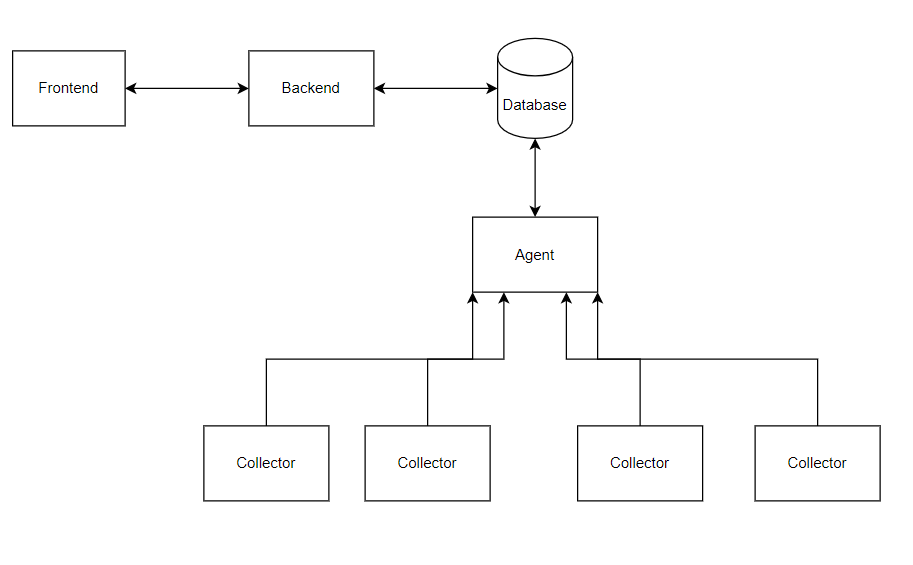
\includegraphics[width=\linewidth]{Images/C4/SystemOverview.png}
% %     \caption{Tổng quan hệ thống}
% % \end{figure}
% % Hệ thống sẽ bao gồm các phần chính :
% % \begin{itemize}
% %     \item Ứng dụng Web bao gồm Backend và Frontend.
% %     \item Công cụ thu thập và xử lý dữ liệu (Agent - Collector)
% %     \item Cơ sở dữ liệu
% % \end{itemize}

% \subsubsection{Module của hệ thống}
% \noindent Nhóm tác giả dựa theo những chức năng chính của hệ thống chia thành các module như sau:
% \begin{enumerate}
%     \item \textbf{Module Giám sát Tài sản CNTT} \\  
%     Tính năng chính:
%     \begin{itemize}[label=--]
%         \item Chịu trách nhiệm thu thập, xử lý và hiển thị dữ liệu giám sát thời gian thực về tình trạng hoạt động của tài sản CNTT trong hệ thống.
%     \end{itemize}
%     Tính năng cụ thể:
%     \begin{itemize}[label=--]
%         \item Hiển thị thông tin cấu hình phần cứng: CPU, RAM, ổ đĩa, card mạng, GPU.
%         \item Hiển thị trạng thái hoạt động thời gian thực:
%         \begin{itemize}[label=\textbullet]
%             \item Hiệu suất sử dụng CPU (\%)
%             \item Bộ nhớ RAM sử dụng
%             \item Thời gian hoạt động (Uptime)
%             \item Tình trạng ổ đĩa (Dung lượng trống)
%             \item Tình trạng mạng (Tốc độ mạng)
%         \end{itemize}
%         \item Hiển thị danh sách ứng dụng đã cài đặt: Phân loại nhà phát hành, phiên bản, kích cỡ.
%         \item Hiển thị biểu đồ theo dõi hiệu suất theo thời gian
%         \item Cảnh báo sự cố và vượt ngưỡng:
%         \begin{itemize}[label=\textbullet]
%             \item Cảnh báo ngay khi giá trị giám sát vượt quá ngưỡng an toàn đã cấu hình (ví dụ: CPU > 90\% trong 5 phút liên tiếp).
%         \end{itemize}
%         \item Dự đoán và cảnh báo sớm:
%         \begin{itemize}[label=\textbullet]
%             \item Phân tích chuỗi thời gian dữ liệu hoạt động (time-series).
%             \item Dự đoán thông số vận hành trong tương lai gần (ví dụ: 15 - 30 phút tiếp theo) bằng mô hình LSTM.
%             \item Cảnh báo sớm nếu giá trị dự đoán sẽ vượt ngưỡng an toàn, giúp phòng ngừa sự cố.
%         \end{itemize}
%     \end{itemize}
%     \item \textbf{Module Quản lý Vòng đời Tài sản} \\
%     Chức năng chính:    
%     \begin{itemize}[label=--]
%         \item Quản lý toàn bộ vòng đời của tài sản, từ mua sắm, triển khai, sử dụng, bảo trì đến thanh lý.
%     \end{itemize}
%     Tính năng cụ thể:
%     \begin{itemize}[label=--]
%         \item Theo dõi lịch sử tài sản:
%         \begin{itemize}[label=\textbullet]
%             \item Ghi nhận lịch sử thay đổi, di chuyển, nâng cấp của từng tài sản.
%         \end{itemize}
%         \item Lập kế hoạch và theo dõi tiến độ bảo trì:
%         \begin{itemize}[label=\textbullet]
%             \item Thiết lập lịch bảo trì định kỳ.
%             \item Theo dõi tiến độ thực hiện bảo trì, kiểm tra tình trạng sau bảo trì.
%         \end{itemize}
%         \item Xử lý quy trình thanh lý tài sản:
%         \begin{itemize}[label=\textbullet]
%             \item Quản lý yêu cầu, phê duyệt và thực hiện quy trình thanh lý tài sản hết vòng đời.
%             \item Ghi nhận tình trạng tài sản tại thời điểm thanh lý.
%         \end{itemize}
%     \end{itemize}
%     \item \textbf{Module Quản lý Dữ liệu Phần cứng và Phần mềm} \\
%     Tính năng chính:
%     \begin{itemize}[label=--]
%         \item Quản lý thông tin chi tiết về phần cứng và phần mềm của từng tài sản trong hệ thống.
%     \end{itemize}
%     Tính năng cụ thể:
%     \begin{itemize}[label=--]
%         \item Lưu trữ và cập nhật thông tin phần cứng:
%         \begin{itemize}[label=\textbullet]
%             \item Nhà sản xuất (Manufacturer)
%             \item Model sản phẩm
%             \item Số serial (Serial Number)
%             \item Cấu hình chi tiết (CPU, RAM, ổ đĩa, GPU, card mạng)
%         \end{itemize}
%         \item Lưu trữ và cập nhật thông tin phần mềm:
%         \begin{itemize}[label=\textbullet]
%             \item Tên phần mềm
%             \item Phiên bản (Version)
%             \item Thông tin giấy phép sử dụng (Mã giấy phép, Ngày hết hạn)
%         \end{itemize}
%         \item Tìm kiếm, lọc và báo cáo dữ liệu:
%         \begin{itemize}[label=\textbullet]
%             \item Tìm kiếm theo nhiều tiêu chí: nhà sản xuất, loại phần cứng, loại phần mềm, trạng thái license,...
%             \item Lọc dữ liệu theo điều kiện tùy chỉnh.
%             \item Xuất báo cáo tổng hợp phần cứng/phần mềm phục vụ kiểm kê, kiểm toán tài sản.
%         \end{itemize}
%     \end{itemize}
%     \item \textbf{Module Cảnh báo} \\
%     Chức năng chính:
%     \begin{itemize}[label=--]
%         \item Quản lý việc tạo, gửi và theo dõi các cảnh báo liên quan đến tình trạng tài sản CNTT.
%     \end{itemize}
%     Chức năng cụ thể:
%     \begin{itemize}[label=--]
%         \item Cấu hình loại cảnh báo và ngưỡng cảnh báo:
%         \begin{itemize}[label=\textbullet]
%             \item Thiết lập các loại cảnh báo (CPU quá tải, RAM đầy, ổ đĩa sắp đầy).
%             \item Xác định các ngưỡng giá trị cụ thể để kích hoạt cảnh báo.
%         \end{itemize}
%         \item Gửi thông báo cảnh báo:
%         \begin{itemize}[label=\textbullet]
%             \item Gửi thông báo cho người dùng qua email hoặc thông báo nội bộ trên hệ thống (push notification).
%         \end{itemize}
%         \item Theo dõi và quản lý lịch sử cảnh báo:
%         \begin{itemize}[label=\textbullet]
%             \item Lưu trữ toàn bộ lịch sử cảnh báo.
%             \item Ghi nhận thông tin chi tiết: thời gian, đối tượng tài sản, mức độ cảnh báo.
%         \end{itemize}
%     \end{itemize}
%     \item \textbf{Module Quản lý đơn đặt hàng} \\
%     Chức năng chính:
%     \begin{itemize}[label=--]
%         \item Cung cấp các tính năng để tạo mới, quản lý và theo dõi các đơn đặt hàng tài sản CNTT từ nhà cung cấp.
%     \end{itemize}
%     Chức năng cụ thể:
%     \begin{itemize}[label=--]
%         \item Tạo và quản lý đơn đặt hàng:
%         \begin{itemize}[label=\textbullet]
%             \item Khởi tạo đơn hàng cho tài sản CNTT (phần cứng, phần mềm, dịch vụ).
%             \item Theo dõi nhà cung cấp, tình trạng đơn hàng và thời gian giao nhận.
%         \end{itemize}
%         \item Lưu trữ lịch sử giao dịch mua sắm:
%         \begin{itemize}[label=\textbullet]
%             \item Ghi nhận chi tiết các giao dịch mua sắm.
%             \item Cập nhật trạng thái giao hàng theo từng đơn hàng.
%         \end{itemize}
%     \end{itemize}
% \end{enumerate}

% %%%%%%%%%%%%%%%%%%%%%%%%%%%%%%%%%
% \subsection{Yêu cầu chức năng và phi chức năng}
% \subsubsection{Yêu cầu chức năng}
% \begin{enumerate}
%     \item \textbf{Giám sát tài sản}
%     \begin{itemize}[label=--]
%         \item Hệ thống phải có chức năng theo dõi và giám sát tất cả tài sản CNTT trong thời gian thực.
%         \item Cung cấp báo cáo tình trạng của tài sản (tài sản vật lý, phần mềm, tài sản ảo)
%         \item Hệ thống cần có khả năng phát hiện các thay đổi trạng thái của tài sản (như bị hỏng, lỗi kết nối, hoặc sử dụng không hợp lý).
%         \item Dự báo hiệu suất hoạt động của tài sản.
%         \item Nhóm người dùng:
%         \begin{itemize}[label=\textbullet]
%             \item Nhân viên IT: Theo dõi hoạt động tài sản, phát hiện lỗi và sự cố kịp thời để xử lý.
%             \item Quản trị viên hệ thống: Đảm bảo các tài sản hoạt động hiệu quả, cấu hình cảnh báo và theo dõi các vấn đề hệ thống phát sinh.
%         \end{itemize}
%     \end{itemize}
%     \item \textbf{Quản lý vòng đời tài sản}
%     \begin{itemize}[label=--]
%         \item Hỗ trợ quản lý toàn bộ vòng đời của tài sản, từ khi mua, triển khai, sử dụng, bảo trì, đến khi thanh lý.
%         \item Ghi lại lịch sử của từng tài sản bao gồm các sự kiện quan trọng như bảo trì, sửa chữa và thay đổi quyền sở hữu.
%         \item Đề xuất thời điểm bảo trì hoặc thay thế tài sản dựa trên dữ liệu hiệu suất và tình trạng tài sản.
%         \item Nhóm người dùng:
%         \begin{itemize}[label=\textbullet]
%            \item Quản lý: Theo dõi vòng đời của tài sản từ khi mua sắm, sử dụng, bảo trì đến khi thanh lý, đảm bảo quản lý chi phí hiệu quả.
%            \item Nhân viên IT: Thực hiện các hoạt động bảo trì và quản lý tài sản trong các giai đoạn khác nhau.

%         \end{itemize}
%     \end{itemize}
%     \item \textbf{Quản lý dữ liệu phần cứng và phần mềm}
%     \begin{itemize}[label=--]
%         \item Hệ thống phải hỗ trợ lưu trữ thông tin cấu hình chi tiết của các tài sản phần cứng và phần mềm.
%         \item Hỗ trợ ánh xạ giữa các tài sản với nhau để biết được các tài sản nào liên quan và phụ thuộc lẫn nhau (như máy tính và phần mềm cài đặt trên máy tính đó).
%         \item Nhóm người dùng:
%         \begin{itemize}[label=\textbullet]
%             \item Nhân viên IT: Cài đặt, cập nhật và quản lý phần cứng, phần mềm.
%             \item Quản trị viên hệ thống: Quản lý cấu hình và trạng thái của hệ thống, bảo đảm tuân thủ các chính sách cấp phép.
 
%         \end{itemize}
%     \end{itemize}
%     \item \textbf{Cảnh báo}
%     \begin{itemize}[label=--]
%         \item Tự động gửi cảnh báo khi có vấn đề liên quan đến tài sản (bảo trì, quá hạn, hiệu suất vượt ngưỡng, lỗi).
%         \item Cho phép tùy chỉnh các quy tắc và ngưỡng cảnh báo.
%         \item Hỗ trợ gửi thông báo qua nhiều kênh (email, SMS, hoặc ứng dụng di động)
%         \item Nhóm người dùng:
%         \begin{itemize}[label=\textbullet]
%             \item Nhân viên IT: Nhận thông báo về các sự cố hoặc thay đổi cấu hình đột ngột, từ đó kịp thời xử lý.
%             \item Quản trị viên hệ thống: Theo dõi và giải quyết các sự cố xảy ra trong quá trình vận hành tài sản.
      
%         \end{itemize}
%     \end{itemize}
%     \item \textbf{Quản lý đơn đặt đặt hàng}
%     \begin{itemize}[label=--]
%         \item Cung cấp các tính năng để tạo, quản lý và theo dõi các đơn đặt hàng tài sản CNTT từ nhà cung cấp.
%         \item Lưu trữ lịch sử các giao dịch mua sắm và tình trạng giao hàng.
%         \item Nhóm người dùng:
%         \begin{itemize}[label=\textbullet]
%             \item Quản lý: Theo dõi đơn đặt hàng, nhà cung cấp, và chi phí liên quan.
%         \end{itemize}
%     \end{itemize}
% \end{enumerate}
% \subsubsection{Yêu cầu phi chức năng}
% \begin{enumerate}
%     \item \textbf{Hiệu suất (Performance)} \\
%     Đảm bảo hệ thống hoạt động nhanh và mượt mà, đáp ứng kịp thời các yêu cầu của người dùng.
%     \begin{table}[H]
%         \centering
%         \caption{Yêu cầu phi chức năng về hiệu suất}
%         \begin{tabular}{|p{3cm}|p{4cm}|p{6cm}|}
%             \hline
%             \textbf{Yêu cầu} & \textbf{Đặc tả} & \textbf{Các hệ thống khác} \\
%             \hline
%             Thời gian phản hồi & Dưới 3 giây để phản hồi các yêu cầu từ người dùng & 
%             \begin{minipage}[t]{6cm}
%             \setlength{\itemindent}{0pt}
%             \setlength{\leftskip}{0pt}
%             \begin{itemize}[leftmargin=*,itemsep=0pt,topsep=0pt,label=--]
%                 \item InvGate Insight có thời gian phản hồi trung bình dưới 1 giây cho các yêu cầu thông thường.
%                 \item ManageEngine có thời gian phản hồi dưới 2 giây, phụ thuộc vào số lượng tài sản và cấu hình máy chủ.
%                 \item ServiceNow có thời gian phản hồi từ 2-3 giây khi quản lý lượng tài sản lớn.
%             \end{itemize}
%             \end{minipage} \\
%             \hline
%             Tốc độ xử lý tài sản & Xử lý và hiển thị thông tin của ít nhất 8.000 tài sản trong vòng 1 phút &
%             \begin{minipage}[t]{6cm}
%             \setlength{\itemindent}{0pt}
%             \setlength{\leftskip}{0pt}
%             \begin{itemize}
%             [leftmargin=*,itemsep=0pt,topsep=0pt,label=--]
%                 \item  InvGate Insight có khả năng xử lý và hiển thị thông tin của 10.000 tài sản trong vòng 1 phút.
%                 \item ManageEngine cũng hỗ trợ xử lý hàng nghìn tài sản. Theo một số đánh giá từ người dùng, hệ thống có thể xử lý khoảng 8.000 - 10.000 tài sản trong dưới 60 giây.
%             \end{itemize}
%             \end{minipage} \\
%             \hline
%             Khả năng xử lý đồng thời & Hỗ trợ ít nhất 500 yêu cầu đồng thời mà không giảm hiệu suất & 
%             \begin{minipage}[t]{6cm}
%             \setlength{\itemindent}{0pt}
%             \setlength{\leftskip}{0pt}
%             \begin{itemize}
%             [leftmargin=*,itemsep=0pt,topsep=0pt,label=--]
%                 \item Các hệ thống lớn như ServiceNow ITAM phải hỗ trợ nhiều người dùng đồng thời mà không ảnh hưởng đến tốc độ.
%             \end{itemize}
%             \end{minipage} \\
%             \hline
%         \end{tabular}
        
%     \end{table}

%     \item \textbf{Khả năng mở rộng (Scalability)} \\
%     Hệ thống phải có khả năng mở rộng theo yêu cầu của tổ chức.
%     \begin{table}[H]
%         \centering
%         \caption{Yêu cầu phi chức năng về Khả năng mở rộng}
%         \begin{tabular}{|p{3cm}|p{4cm}|p{6cm}|}
%             \hline
%             \textbf{Yêu cầu} & \textbf{Đặc tả} & \textbf{Các hệ thống khác} \\
%             \hline
%             Số lượng tài sản có thể quản lý & Hỗ trợ quản lý ít nhất 500 tài sản, mở rộng lên đến 100.000 tài sản & 
%             \begin{minipage}[t]{6cm}
%             \setlength{\itemindent}{0pt}
%             \setlength{\leftskip}{0pt}
%             \begin{itemize}[leftmargin=*,itemsep=0pt,topsep=0pt,label=--]
%                 \item InvGate Insight có khả năng mở rộng từ 500 tài sản lên tới 100.000 tài sản, phù hợp với nhu cầu mở rộng trong các tổ chức lớn.
%                 \item ManageEngine cũng cung cấp khả năng mở rộng từ vài trăm tới hàng chục nghìn tài sản.
%                 \item ServiceNow nổi bật với khả năng mở rộng lớn hơn, hỗ trợ lên tới hàng trăm nghìn tài sản cho các tập đoàn toàn cầu.
%             \end{itemize}
%             \end{minipage} \\
%             \hline
%             Khả năng tăng số lượng người dùng & Hỗ trợ tăng số lượng người dùng lên ít nhất 1.000 người hoạt động cùng lúc &
%             \begin{minipage}[t]{6cm}
%             \setlength{\itemindent}{0pt}
%             \setlength{\leftskip}{0pt}
%             \begin{itemize}
%             [leftmargin=*,itemsep=0pt,topsep=0pt,label=--]
%                 \item ServiceNow ITAM là hệ thống được thiết kế cho tổ chức lớn, với nhiều người dùng đồng thời.
%             \end{itemize}
%             \end{minipage} \\
%             \hline
%         \end{tabular}
        
%     \end{table}
%     \item \textbf{Tính sẵn sàng và độ tin cậy (Availability \& Reliability)} \\
%     Đảm bảo hệ thống luôn sẵn sàng hoạt động, hạn chế thời gian ngừng và phục hồi nhanh chóng khi gặp sự cố.
%     \begin{table}[H]
%         \centering
%         \caption{Yêu cầu phi chức năng về Tính sẵn sàng và độ tin cậy}
%         \begin{tabular}{|p{3cm}|p{4cm}|p{6cm}|}
%             \hline
%             \textbf{Yêu cầu} & \textbf{Đặc tả} & \textbf{Các hệ thống khác} \\
%             \hline
%             Thời gian hoạt động của hệ thống (Uptime) & 99.9\% uptime với thời gian ngừng tối đa 60 phút mỗi tháng & 
%             \begin{minipage}[t]{6cm}
%             \setlength{\itemindent}{0pt}
%             \setlength{\leftskip}{0pt}
%             \begin{itemize}[leftmargin=*,itemsep=0pt,topsep=0pt,label=--]
%                 \item InvGate Insight cam kết đạt 99.9\% uptime, tức là thời gian ngừng tối đa chỉ khoảng 43.8 phút mỗi tháng.
%                 \item ManageEngine cũng đạt 99.9\% uptime.
%                 \item  ServiceNow ITAM đặt ra tiêu chuẩn cao với 99.99\% uptime.
%             \end{itemize}
%             \end{minipage} \\
%             \hline
%             Khả năng phục hồi (Recovery Time Objective) & Hệ thống phải phục hồi trong vòng 1 giờ sau sự cố &
%             \begin{minipage}[t]{6cm}
%             \setlength{\itemindent}{0pt}
%             \setlength{\leftskip}{0pt}
%             \begin{itemize}
%             [leftmargin=*,itemsep=0pt,topsep=0pt,label=--]
%                 \item ManageEngine có khả năng khôi phục nhanh chóng nhờ các cơ chế sao lưu mạnh mẽ.
%             \end{itemize}
%             \end{minipage} \\
%             \hline
%         \end{tabular}
        
%     \end{table}
%     \item \textbf{Bảo mật (Security)} \\
%     Đảm bảo dữ liệu tài sản và quyền truy cập được bảo vệ an toàn trước các mối đe dọa bảo mật.
%     \begin{table}[H]
%         \centering
%         \caption{Yêu cầu phi chức năng về Bảo mật}
%         \begin{tabular}{|p{3cm}|p{4cm}|p{6cm}|}
%             \hline
%             \textbf{Yêu cầu} & \textbf{Đặc tả} & \textbf{Các hệ thống khác} \\
%             \hline
%             Bảo mật truy cập & Hỗ trợ xác thực đa yếu tố (MFA) và mã hóa dữ liệu đầu cuối & Hệ thống hỗ trợ xác thực đa yếu tố (MFA) và mã hóa dữ liệu, giúp bảo vệ quyền truy cập và đảm bảo dữ liệu tài sản luôn an toàn. Đây là tiêu chuẩn bảo mật phổ biến cho các hệ thống quản lý tài sản CNTT lớn. \\
%             \hline
%         \end{tabular}
        
%     \end{table}
%     \item \textbf{Khả năng tích hợp (Integration)}
%     \begin{table}[H]
%         \centering
%         \caption{Yêu cầu phi chức năng về Khả năng tích hợp}
%         \begin{tabular}{|p{3cm}|p{4cm}|p{6cm}|}
%             \hline
%             \textbf{Yêu cầu} & \textbf{Đặc tả} & \textbf{Các hệ thống khác} \\
%             \hline
%             Tích hợp API & Hỗ trợ API cho phép tích hợp hệ thống với các ứng dụng quản lý khác. & InvGate Insight hỗ trợ API miễn phí để tích hợp với các hệ thống quản lý khác. Điều này giúp doanh nghiệp dễ dàng đồng bộ hóa dữ liệu giữa các hệ thống, tối ưu hóa quy trình quản lý tài sản.\\
%             \hline
%             Tích hợp bên thứ ba & Tích hợp với các công cụ bên thứ ba & ServiceNow có khả năng tích hợp mạnh mẽ với nhiều công cụ bên thứ ba như AirWatch hoặc SentinelOne, cho phép kết nối và chia sẻ dữ liệu dễ dàng với các hệ thống bảo mật và quản lý khác. \\
%             \hline
%         \end{tabular}
        
%     \end{table}
% \end{enumerate}
% %%%%%%%%%%%%%%%%%%%%%%%%%%%%%%%%%
% %%%%%%%%%%%%%%%%%%%%%%%%%%%%%%%%%
% \subsubsection{Yêu cầu dữ liệu}
% \begin{enumerate}
%     %%%%%
%     \item \textbf{Dữ liệu tài sản}:
%         \begin{itemize}[label=--]
%             \item Mã tài sản (Mã tài sản sẽ thay đổi theo từng loại tài sản, ví dụ Laptop có thể được kí hiệu là COM001)
%             \item Tên tài sản 
%             \item Loại tài sản (Gồm 3 loại tài sản là phần cứng, phần mềm, máy tính)
%             \item Nhân viên IT quản lý tài sản hiện tại. Một nhân viên IT có thể quản lý nhiều tài sản và một tài sản có thể được quản lý bởi nhiều nhân viên IT
%         \end{itemize}

%     %%%%%
%     \item \textbf{Dữ liệu giám sát thời gian thực}:
%             \begin{itemize}[label=--]
%                 \item Trạng thái hoạt động của tài sản
%                 \item Thời gian hoạt động
%                 \item Mức sử dụng CPU
%                 \item Mức sử dụng RAM
%                 \item Dung lượng ổ đĩa còn trống
%                 \item Ngưỡng của máy tính bao gồm: loại ngưỡng, giá trị ngưỡng, ngày tạo, độ ưu tiên ngưỡng, mã nhân viên điều chỉnh ngưỡng. Ngưỡng này được dùng để tạo cảnh báo cho RAM, CPU, ổ đĩa
%                 \item Sự kiện hệ thống là lỗi khi có sự cố
%                 \begin{itemize}[label=\textbullet]
%                     \item Nhân viên giải quyết lỗi
%                     \item Ngày phát hiện lỗi
%                     \item Loại lỗi gặp 
%                     \item Mã máy tính gặp lỗi
%                     \item Trạng thái giải quyết
%                     \item Thời gian phát hiện và thời gian giải quyết
%                     \item Mô tả lỗi hay sự cố gặp phải là gì.
%                 \end{itemize}
%                 \item Sự kiện hệ thống là cảnh báo khi có dữ liệu vượt ngưỡng
%                 \begin{itemize}[label=\textbullet]
%                     \item Mã ngưỡng
%                     \item Thời gian đưa ra cảnh báo
%                     \item Mức độ nghiêm trọng
%                     \item Khoảng thời gian kiểm tra ngưỡng
%                     \item Loại cảnh báo
%                     \item Mã máy tính bị cảnh báo 
%                 \end{itemize}
%             \end{itemize}
%     %%%%%
%     \item \textbf{Dữ liệu Quản lý vòng đời tài sản}\\
%     \noindent Vòng đời tài sản sẽ bao gồm 4 giai đoạn 
%      \begin{itemize}[label=--]
%         \item Thông tin giai đoạn mua sắm:
%             \begin{itemize}[label=\textbullet]
%                 \item Mã đơn hàng 
%                 \item Nhà cung cấp
%                 \item Giá trị tài sản
%             \end{itemize}
%         \item Thông tin giai đoạn triển khai
%             \begin{itemize}[label=\textbullet]
%                 \item Ví trí triển khai
%                 \item Phòng ban triển khai
%                 \item Ngày triển khai
%                 \item Nhân viên chịu trách nhiệm
%                 \item Trạng thái triển khai (hoàn tất, đang triển khai)
%             \end{itemize}
%         \item Thông tin giai đoạn sử dụng:
%         \begin{itemize}[label=\textbullet]
%            \item Tình trạng sử dụng 
%             \item Ngày bắt đầu sử dụng
%             \item Người sử dụng
%             \item Ngày hết hạn bảo hành
%             \item Phương pháp khấu hao, ngày bắt đầu khấu hao, tổng giá trị khấu hao
%             \item Trạng thái hoạt động
%             \item Giá trị hiện tại của tài sản 
%         \end{itemize}
%         \item Thông tin giai đoạn thanh lý:
%         \begin{itemize}[label=\textbullet]
%             \item Phương thức thanh lý
%             \item Ngày thanh lý
%             \item Trạng thái thanh lý
%             \item Nhà cung cấp dịch vụ thanh lý
%             \item Lý do thanh lý
%             \item Giá bán cuối cùng
%             \item Trạng thái phê duyệt thanh lý
%         \end{itemize}
%     \end{itemize}
%     \noindent Ngoài những thông tin trên còn có các thông tin về \textbf{bảo trì tài sản}:
%     \begin{itemize}[label=--]
%         \item Loại bảo trì (Bảo trì định kỳ, nâng cấp tài sản, bảo trì đột xuất, kiểm tra hệ thống)
%         \item Chu kỳ bảo trì (Hàng tháng, hàng quý, hàng năm)
%         \item Lý do bảo trì (Lỗi, hao mòn, nâng cấp theo yêu cầu)
%         \item Mô tả bảo trì (thông tin này sẽ được sử dụng vào lần bảo trì kế tiếp)
%         \item Nhân viên chịu trách nhiệm bảo trì
%         \item Chi phí bảo trì
%         \item Thời gian bắt đầu và kết thúc bảo trì
%     \end{itemize}
%     %%%%
%     \item \textbf{Dữ liệu Phần cứng và Phần mềm, Máy tính}\\
%     Máy tính, Phần cứng, Phần mềm là các loại đối tượng tài sản cần phải quản lý. Dữ liệu yêu cầu:
%     \begin{itemize}[label=--]
%         \item Thông tin máy tính:
%         \begin{itemize}[label=\textbullet]
%             \item Địa chỉ IP/Mac
%             \item Số serial
%             \item Mẫu máy tính
%             \item Hệ điều hành
%             \item Loại máy tính
%             \item Tình trạng sử dụng máy (đang sử dụng hay không)
%             \item Tên máy tính (tên máy tính đặt theo tên tài khoản nhân viên được công ty cung cấp)
%         \end{itemize}
%         \item Thông tin phần cứng:
%             \begin{itemize}[label=\textbullet]
%                 \item Thông số kỹ thuật chi tiết (CPU, RAM, ổ cứng, card mạng,...)
%                 \item Số serial
%                 \item Phần cứng được chia thành 5 loại là CPU, RAM, Ổ cứng, Card mạng, GPU 
%             \end{itemize}
%         \item Thông tin phần mềm:
%             \begin{itemize}[label=\textbullet]
%                 \item Tên phần mềm
%                 \item Phiên bản
%                 \item Nhà phát hành
%                 \item Ngày cài đặt
%                 \item Dung lượng (nếu có)
%                 \item Một phần mềm có thể có một giấy phép nếu phần mềm này được mua từ bên thứ ba. Phần mềm có thể được cài đặt trên nhiều máy tính. Thông tin giấy phép phần mềm (nếu có) :
%                 \begin{itemize}[label=*]
%                     \item Khóa giấy phép
%                     \item Loại giấy phép
%                     \item Tình trạng sử dụng 
%                     \item Ngày hết hạn giấy phép
%                     \item Ngày mua giấy phép
%                     \item Nhà phát hành
%                 \end{itemize}
%             \end{itemize}
%     \end{itemize}
%     %%%%
%     \item \textbf{Dữ liệu Quản lý đơn đặt hàng}
%     \begin{itemize}[label=--]
%         \item Thông tin đơn đặt hàng:
%         \begin{itemize}[label=\textbullet]
%             \item Mã đơn đặt hàng
%             \item Ngày đặt hàng
%             \item Danh sách sản phẩm
%             \item Tình trạng đơn hàng
%             \item Nhà cung cấp
%         \end{itemize}
%         \item Thông tin thanh toán gồm chi phí đơn hàng, chi phí vận chuyển
%         \item Thông tin nhà cung cấp
%     \end{itemize}
%     \item \textbf{Dữ liệu Quản lý yêu cầu nâng cấp}
%     \begin{itemize}[label=--]
%         \item Mã yêu cầu nâng cấp
%         \item Tên tài sản cần được nâng cấp
%         \item Loại nâng cấp (nâng cấp phần cứng, nâng cấp phần mềm), Chi tiết nâng cấp, tình trạng nâng cấp, thời gian hoàn thành nâng cấp, thời gian tạo yêu cầu nâng cấp
%         \item Nhân viên thực hiện
%         \item Nhân viên IT có thể tạo nhiều yêu cầu nâng cấp
%     \end{itemize}
%     \item \textbf{Dữ liệu người dùng của hệ thống}:\\
%     Người dùng của hệ thống bao gồm : nhân viên IT, quản lý, quản trị viên hệ thống. Dữ liệu của tài khoản người dùng:
%     \begin{itemize}[label=--]
%          \item Mã nhân viên
%          \item Tên đăng nhập, mật khẩu, ngày tạo tài khoản
%          \item Email, số điện thoại
%          \item Vai trò
%     \end{itemize}
% \end{enumerate}

% \subsection{Kết chương}
% \noindent Hệ thống được thiết kế nhằm phục vụ nhu cầu của các doanh nghiệp vừa và nhỏ trong việc phát hiện và quản lý hiệu quả các tài sản CNTT, từ việc giám sát thời gian thực, quản lý vòng đời, đến xử lý sự cố và đưa ra các cảnh báo kịp thời. Ba nhóm đối tượng người dùng chính - quản trị viên hệ thống, nhân viên IT và quản lý - được xác định rõ ràng với các nhiệm vụ và quyền hạn phù hợp, bảo đảm tính linh hoạt và khả năng phân quyền tối ưu. \\  \\
% Các module chính bao gồm:
% \begin{itemize}[label=--]
%     \item \textbf{Module Giám sát tài sản CNTT}, cung cấp khả năng thu thập dữ liệu về cấu hình phần cứng, phần mềm, trạng thái hoạt động và hiệu suất của tài sản.
%     \item \textbf{Module Quản lý vòng đời tài sản}, hỗ trợ quản lý toàn diện các giai đoạn từ mua sắm, triển khai, sử dụng, đến thanh lý tài sản.
%     \item \textbf{Module Quản lý dữ liệu phần cứng và phần mềm}, đảm bảo thông tin chi tiết về tài sản luôn được lưu trữ và cập nhật chính xác.
%     \item \textbf{Module Cảnh báo}, giúp phát hiện và thông báo kịp thời khi có sự cố hoặc khi hiệu suất tài sản vượt ngưỡng an toàn.
%     \item \textbf{Module Quản lý đơn đặt hàng}, hỗ trợ xử lý quy trình mua sắm tài sản một cách hiệu quả.
% \end{itemize}
% Hệ thống cũng được xây dựng trên các yêu cầu chức năng cụ thể như giám sát tài sản, quản lý vòng đời tài sản, và gửi cảnh báo. Các yêu cầu phi chức năng bảo đảm hệ thống có hiệu năng tốt, khả năng mở rộng linh hoạt, tính sẵn sàng cao và bảo mật mạnh mẽ. Những tiêu chí này đã được so sánh với các giải pháp tương tự trên thị trường, như InvGate Insight, ManageEngine, và Service Now, để bảo đảm hệ thống đáp ứng với tiêu chuẩn ngành. \\ \\
% Nhìn chung, hệ thống quản lý tài sản CNTT thời gian thực được đề xuất không chỉ giải quyết được các vấn đề trong quản lý tài sản hiện tại mà còn cung cấp nền tảng vững chắc để đảm bảo hiệu quả và an toàn cho tài sản CNTT của doanh nghiệp.
% \newpage
%  \section{Định hướng phát triển}

\subsection{Tổng kết các giới hạn hiện tại}

Các kết quả thực nghiệm ở Chương 4 đã chứng minh tiềm năng của kiến trúc giám sát lai trong việc kết hợp tốc độ xử lý của detector metric-only với khả năng suy luận ngữ cảnh của RAG và LLM-as-a-Judge. Tuy nhiên, hệ thống hiện tại vẫn tồn tại một số giới hạn cần được tiếp tục hoàn thiện trong các giai đoạn nghiên cứu tiếp theo:

\begin{itemize}
    \item \textbf{Giới hạn về môi trường thực nghiệm:} Pipeline hiện mới chỉ được đánh giá trong môi trường giả lập có kiểm soát thông qua cơ chế phát lại luồng, chưa phải là một triển khai thời gian thực trong môi trường production. Mặc dù cơ chế watermark đã giúp hạn chế việc rò rỉ thông tin từ tương lai khi truy xuất log/trace, hệ thống vẫn cần được kiểm chứng thêm trên các luồng dữ liệu thực hoặc môi trường microservice vận hành liên tục.
    \item \textbf{Thiếu hụt các chỉ số đánh giá chiều sâu của RAG:} Chất lượng của tầng RAG hiện chủ yếu được đánh giá qua các chỉ số vĩ mô như context coverage, số lượng context trung bình và độ trễ truy xuất. Các chỉ số này chưa đo lường sâu mức độ chính xác và đầy đủ của bằng chứng được đưa vào LLM.
    \item \textbf{Chi phí vận hành của Context Rescue:} Cơ chế Context Rescue cho thấy khả năng cải thiện Recall rõ rệt, nhưng đồng thời làm tăng đáng kể số lượng ứng viên, số lần truy xuất ngữ cảnh và số lượt gọi LLM. Do đó, cơ chế này cần được hình thức hóa và kiểm soát chặt chẽ hơn thông qua các ngưỡng kích hoạt và chính sách manual review.
    \item \textbf{Độ ổn định của chiến lược Local-first:} Chiến lược Local-first mới chỉ được kiểm chứng ở mức khả thi về mặt vận hành. Kết quả cho thấy mô hình cục bộ có thể tham gia vào tầng thẩm định, nhưng vẫn bắt buộc phải có cơ chế fallback sang API trong các trường hợp thiếu chắc chắn hoặc đầu ra không đạt yêu cầu. Mô hình cục bộ hiện tại chưa thể thay thế hoàn toàn mô hình API bên ngoài.
\end{itemize}

\subsection{Hình thức hóa và tối ưu cơ chế Context Rescue}

Một định hướng phát triển trọng tâm là xây dựng cơ chế \textbf{Context Rescue} thành một tầng khôi phục ứng viên dựa trên bằng chứng ngữ cảnh một cách có hệ thống. Trong phiên bản hiện tại, Context Rescue được sử dụng để rà soát các cửa sổ metric mà detector chưa đánh dấu là candidate. Nếu log/trace xung quanh cửa sổ đó chứa tín hiệu đủ mạnh, hệ thống sẽ chọn cửa sổ này thành ứng viên cảnh báo để đưa vào quy trình RAG + LLM-as-a-Judge.

Trong giai đoạn tiếp theo, cơ chế này sẽ được mô hình hóa bằng một \textbf{hàm tính điểm Context Rescue (Rescue Score)} kết hợp đa chiều các yếu tố: mức độ nghiêm trọng của log/trace event, độ suy giảm theo thời gian giữa event và metric window, mức độ liên quan về mặt topology giữa service sinh event và service đang được giám sát, cũng như độ tin cậy của nguồn bằng chứng. Một cửa sổ chỉ được promote khi điểm Rescue Score vượt qua một ngưỡng xác định ($\tau$) và có đủ số lượng bằng chứng hỗ trợ (evidence count $\ge m$).

Việc hình thức hóa này giúp hệ thống loại bỏ các quyết định mang tính heuristic, đồng thời cho phép định lượng rõ ràng sự đánh đổi giữa Recall và chi phí vận hành. Các thí nghiệm tiếp theo sẽ tập trung khảo sát sự ảnh hưởng của ngưỡng $\tau$ và $m$ đến số lượng ứng viên được chọn, số lượt gọi LLM phát sinh, cũng như tỷ lệ false positive mới được tạo ra do nhiễu ngữ cảnh.

\subsection{Bổ sung RCA Post-processing Agent cho xử lý hậu kỳ}

Một hướng mở rộng quan trọng nhằm nâng cao tính ứng dụng của đề tài là bổ sung một tác tử xử lý hậu kỳ đứng sau tầng LLM-as-a-Judge. Trong kiến trúc hiện tại, hệ thống chủ yếu dừng lại ở việc đưa ra quyết định phân loại cho từng alert candidate (ví dụ: route alert, suppress hoặc manual review). Tuy nhiên, trong môi trường vận hành thực tế, đội ngũ quản trị (SRE/DevOps) không chỉ cần biết một cảnh báo có hợp lệ hay không, mà còn cần hiểu cảnh báo đó thuộc sự cố nào, bằng chứng chính là gì, nguyên nhân khả dĩ là gì và hành động khắc phục ra sao.

RCA Post-processing Agent được đề xuất như một tầng xử lý hậu kỳ, nhận đầu vào gồm các cảnh báo đã được xác nhận, metric snapshot, log/trace context, quyết định của LLM-as-a-Judge và audit metadata. Từ các thông tin này, agent sẽ thực hiện các tác vụ: gom nhóm các cảnh báo liên quan thành một sự cố, tóm tắt bằng chứng vận hành, sinh giả thuyết nguyên nhân gốc rễ , đề xuất hành động xử lý và lưu lại bộ nhớ phản hồi cho các lần phân tích sau.

Đầu ra của agent sẽ được ràng buộc ở dạng có cấu trúc, bao gồm: affected service, severity, root-cause hypothesis, supporting evidence, missing evidence, recommended actions và feedback label. Cách tổ chức này giúp hệ thống chuyển dịch từ bài toán thẩm định cảnh báo đơn lẻ  sang bài toán hỗ trợ chẩn đoán và hiểu sự cố, phù hợp hơn với mục tiêu AIOps trong môi trường cloud/server.

Luồng mở rộng có thể được mô tả như sau:
% Đảm bảo đã khai báo \usepackage{tikz} và \usetikzlibrary{positioning, arrows.meta} ở phần preamble của tài liệu

\begin{figure}[htbp]
    \centering
    \resizebox{\textwidth}{!}{
    \begin{tikzpicture}[
        node distance=0.8cm and 1.2cm,
        box/.style={
            rectangle, 
            draw, 
            rounded corners, 
            align=center,
            minimum width=3.2cm, 
            minimum height=1.0cm,
            font=\small\bfseries, 
            fill=gray!5, 
            thick
        },
        input_box/.style={
            rectangle, 
            draw, 
            align=center,
            minimum width=3.2cm, 
            minimum height=1.0cm,
            font=\small\bfseries, 
            fill=blue!5, 
            thick
        },
        agent_box/.style={
            rectangle, 
            draw, 
            rounded corners=2mm,
            align=center,
            minimum width=3.8cm, 
            minimum height=1.1cm,
            font=\small\bfseries, 
            fill=red!5, % Đổi màu nền đỏ nhạt để làm nổi bật tác tử xử lý hậu kỳ
            draw=red!60!black,
            thick
        },
        arrow/.style={-{Stealth}, thick}
    ]

        % Cụm dữ liệu đầu vào (Xếp chồng hàng dọc bên trái để tiết kiệm không gian ngang)
        \node[input_box] (alert) {Validated Alert\\ \textmd{\small(Cảnh báo hợp lệ)}};
        \node[input_box, below=0.4cm of alert] (context) {Retrieved Context\\ \textmd{\small(Ngữ cảnh truy xuất)}};
        \node[input_box, below=0.4cm of context] (audit) {Audit Metadata\\ \textmd{\small(Siêu dữ liệu lưu vết)}};

        % Điểm gộp luồng trung gian (Hộp đứt nét bao quanh dữ liệu đầu vào)
        \coordinate[right=0.6cm of context] (merge);

        % Thành phần xử lý trung tâm (Agent)
        \node[agent_box, right=1.5cm of context] (agent) {RCA Post-processing Agent\\ \textmd{\small(Tác tử xử lý hậu kỳ RCA)}};

        % Đầu ra cuối cùng
        \node[input_box, right=1.5cm of agent] (report) {Incident Report\\ \textmd{\small(Báo cáo sự cố)}};

        % Vẽ các đường kết nối mũi tên
        \draw[thick] (alert) -| (merge);
        \draw[arrow] (context) -- (agent);
        \draw[thick] (audit) -| (merge);
        
        \draw[arrow] (agent) -- (report);

    \end{tikzpicture}
    }
    \vspace{0.3cm}
    \caption{Quy trình tổng hợp và xử lý hậu kỳ cấu trúc báo cáo sự cố tự động}
    \label{fig:rca_post_processing_flow}
\end{figure}
\subsection{Mở rộng bộ chỉ số đánh giá chất lượng ngữ cảnh và bằng chứng}

Bên cạnh việc đo lường chất lượng cảnh báo bằng các chỉ số kinh điển như Precision, Recall, F1-score và FPR, các giai đoạn sau cần đánh giá sâu hơn chất lượng bằng chứng mà tầng RAG cung cấp cho LLM. Các chỉ số hiện tại chưa trả lời đầy đủ câu hỏi liệu context được truy xuất có thực sự mang tính quyết định đến sự cố hay không.

Do đó, nghiên cứu sẽ bổ sung một bộ chỉ số đánh giá chuyên sâu cho tầng Retrieval, bao gồm:
\begin{itemize}
    \item \textbf{Evidence hit@k:} Đo lường tỷ lệ top-k context truy xuất được có chứa log/trace thực sự liên quan đến fault injection.
    \item \textbf{Service match rate:} Đo lường mức độ trùng khớp về service/pod giữa context được truy xuất và alert candidate.
    \item \textbf{Time-window match:} Đo lường mức độ gần gũi về mặt thời gian giữa context và metric window.
    \item \textbf{Unsupported decision rate:} Đo lường tỷ lệ các trường hợp LLM đưa ra quyết định "route alert" nhưng thiếu bằng chứng hỗ trợ rõ ràng trong context được cung cấp.
\end{itemize}

Bộ chỉ số này sẽ giúp đánh giá RAG không chỉ đơn thuần là một thành phần truy xuất văn bản , mà là một cơ chế cung cấp bằng chứng vận hành cho quá trình thẩm định cảnh báo.

\subsection{Mở rộng thực nghiệm và triển khai trên luồng dữ liệu thời gian thực}

Hướng phát triển cuối cùng là mở rộng thực nghiệm sang các môi trường microservice hoặc cloud-native benchmark có khả năng chủ động thu thập đồng thời metric, log, trace và event. Các môi trường như TrainTicket, Online Boutique hoặc Sock Shop có thể được triển khai kết hợp với Prometheus, OpenTelemetry và Jaeger/Tempo để tạo ra dữ liệu telemetry sát với vận hành thực tế. Khi kết hợp với các công cụ tiêm lỗi, hệ thống có thể đánh giá toàn diện các tình huống như network delay, CPU contention, memory pressure, service unavailable hoặc database latency.

Bên cạnh đó, cần tiếp tục hoàn thiện cơ chế xử lý theo luồng. Cơ chế streaming replay hiện tại giúp kiểm soát thứ tự thời gian, nhưng chưa phản ánh đầy đủ các thách thức của production streaming như sự kiện đến không theo thứ tự, backpressure, độ trễ hàng đợi, hay cơ chế thử lại . Các giai đoạn sau có thể bổ sung hàng đợi ưu tiên, scheduler bất đồng bộ, bộ nhớ đệm nhiều tầng và cơ chế defer/manual review cho các alert không đủ ngân sách LLM tại thời điểm xử lý.

Cuối cùng, chiến lược Local-first cần được đánh giá với các mô hình cục bộ lớn hơn hoặc được tối ưu hóa, đồng thời so sánh với các API fallback khác nhau. Mục tiêu tối thượng không phải là thay thế hoàn toàn API bên ngoài, mà là xác định chiến lược điều phối hợp lý giữa mô hình cục bộ, API fallback, semantic cache và manual review để tối ưu hóa bài toán đánh đổi giữa Chi phí - Độ trễ - Độ chính xác.

% \subsection{ Phân tích}
% \subsubsection{ Mô hình hoá quy trình nghiệp vụ}
% \begin{enumerate}
% %----------%
%     \item \textbf{Giám sát tài sản}
%     \begin{figure}[H]
%     \centering
%     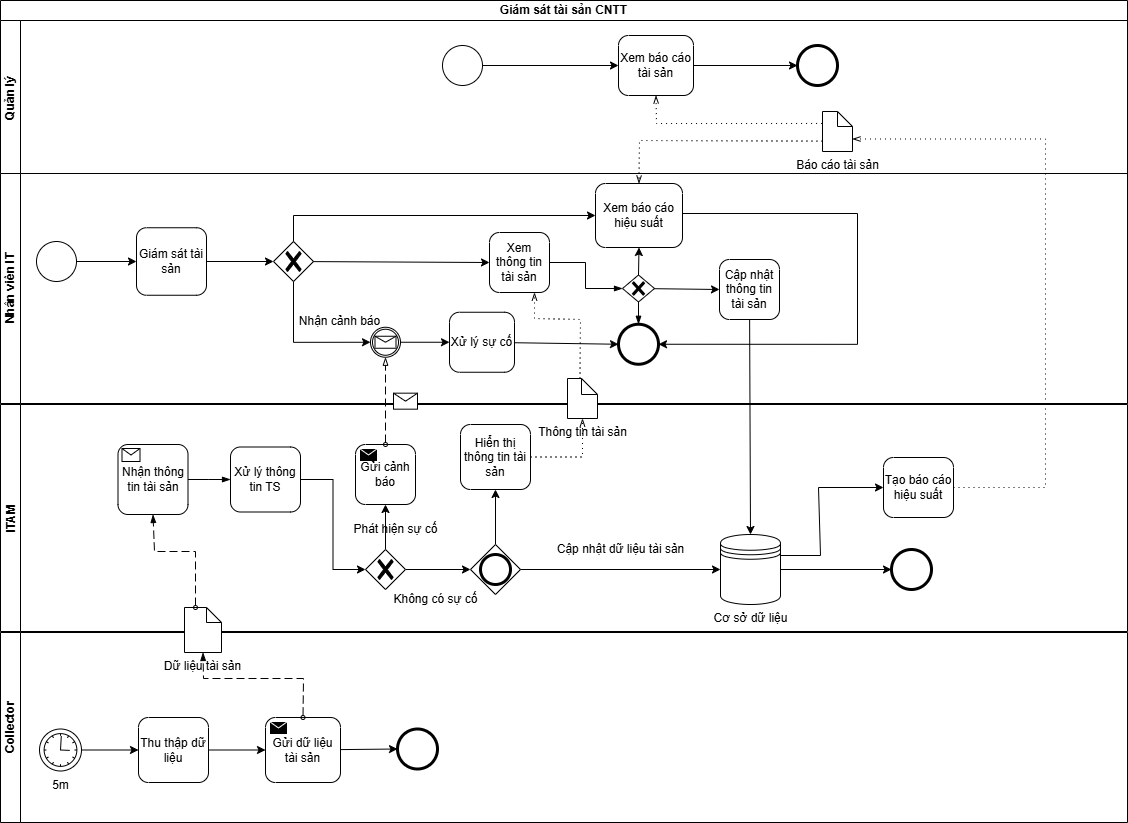
\includegraphics[width=\linewidth]{Images/C5/BPMN/RITAM-Giám sát Tài sản CNTT.drawio.png}
%     \vspace{0.5cm}
%     \caption{Mô hình hóa nghiệp vụ giám sát tài sản}
% \end{figure}
%      \begin{itemize}[label=--]
%         \item \textbf{Thu thập dữ liệu tài sản:} 
%         \begin{itemize}[label=\textbullet]
%             \item Cứ 5 phút, phần mềm Collector được cài đặt tại máy tính (bao gồm cả máy tính để bàn và máy tính xách tay) thu thập dữ liệu về cấu hình phần cứng, phần mềm, hiệu năng (RAM, CPU, bộ nhớ).
%             \item Dữ liệu mà Collector thu thập được sẽ gửi đến hệ thống quản lý tài sản - ITAM .
%         \end{itemize}
%         \item \textbf{Xử lý và quản lý dữ liệu tài sản CNTT:}
%         \begin{itemize}[label=\textbullet]
%             \item Hệ thống ITAM tiếp nhận dữ liệu tài sản CNTT theo thời gian thực từ Collector.
%             \item Hệ thống sẽ xử lý, phân tích và lưu trữ thông tin tài sản vào cơ sở dữ liệu. Vì sẽ có nhiều thông tin từ nhiều tài sản gửi lên cùng một lúc nên hệ thống sẽ sử dụng Kafka như trung gian để tổng hợp, phân phối dữ liệu.
%             \item Trong trường hợp không có sự cố, thì dữ liệu tài sản sẽ được cập nhật vào cơ sở dữ liệu, đồng thời sẽ được hiển thị ở màn hình nhân viên IT.
%         \end{itemize}
%         \item \textbf{Xử lý sự cố tài sản}
%         \begin{itemize}[label=\textbullet]
%             \item Qua quá trình xử lý dữ liệu từ tài sản, nếu phát hiện sự cố, hệ thống ITAM sẽ gửi cảnh báo đến Nhân viên IT. Sau đó Nhân viên IT bắt đầu quy trình xử lý sự cố.
%         \end{itemize}       
%         \item \textbf{Giám sát tài sản}
%         \begin{itemize}[label=\textbullet]
%             \item Trong quy trình giám sát tài sản, nhân viên IT có thể xem thông tin chi tiết tài sản, báo cáo hiệu suất, cập nhật thông tin tài sản, và xử lý sự cố khi có cảnh báo.
%             \item Quản lý cũng có thể xem các bảng tổng quan về tình trạng tài sản
%         \end{itemize}
        
%     \end{itemize}
% %----------%
%     \item \textbf{Quản lý vòng đời tài sản}\\
%     Vòng đời tài sản bao gồm các giai đoạn như sau: mua sắm, triển khai, sử dụng, thanh lý.
%      \begin{figure}[H]
%     \centering
%     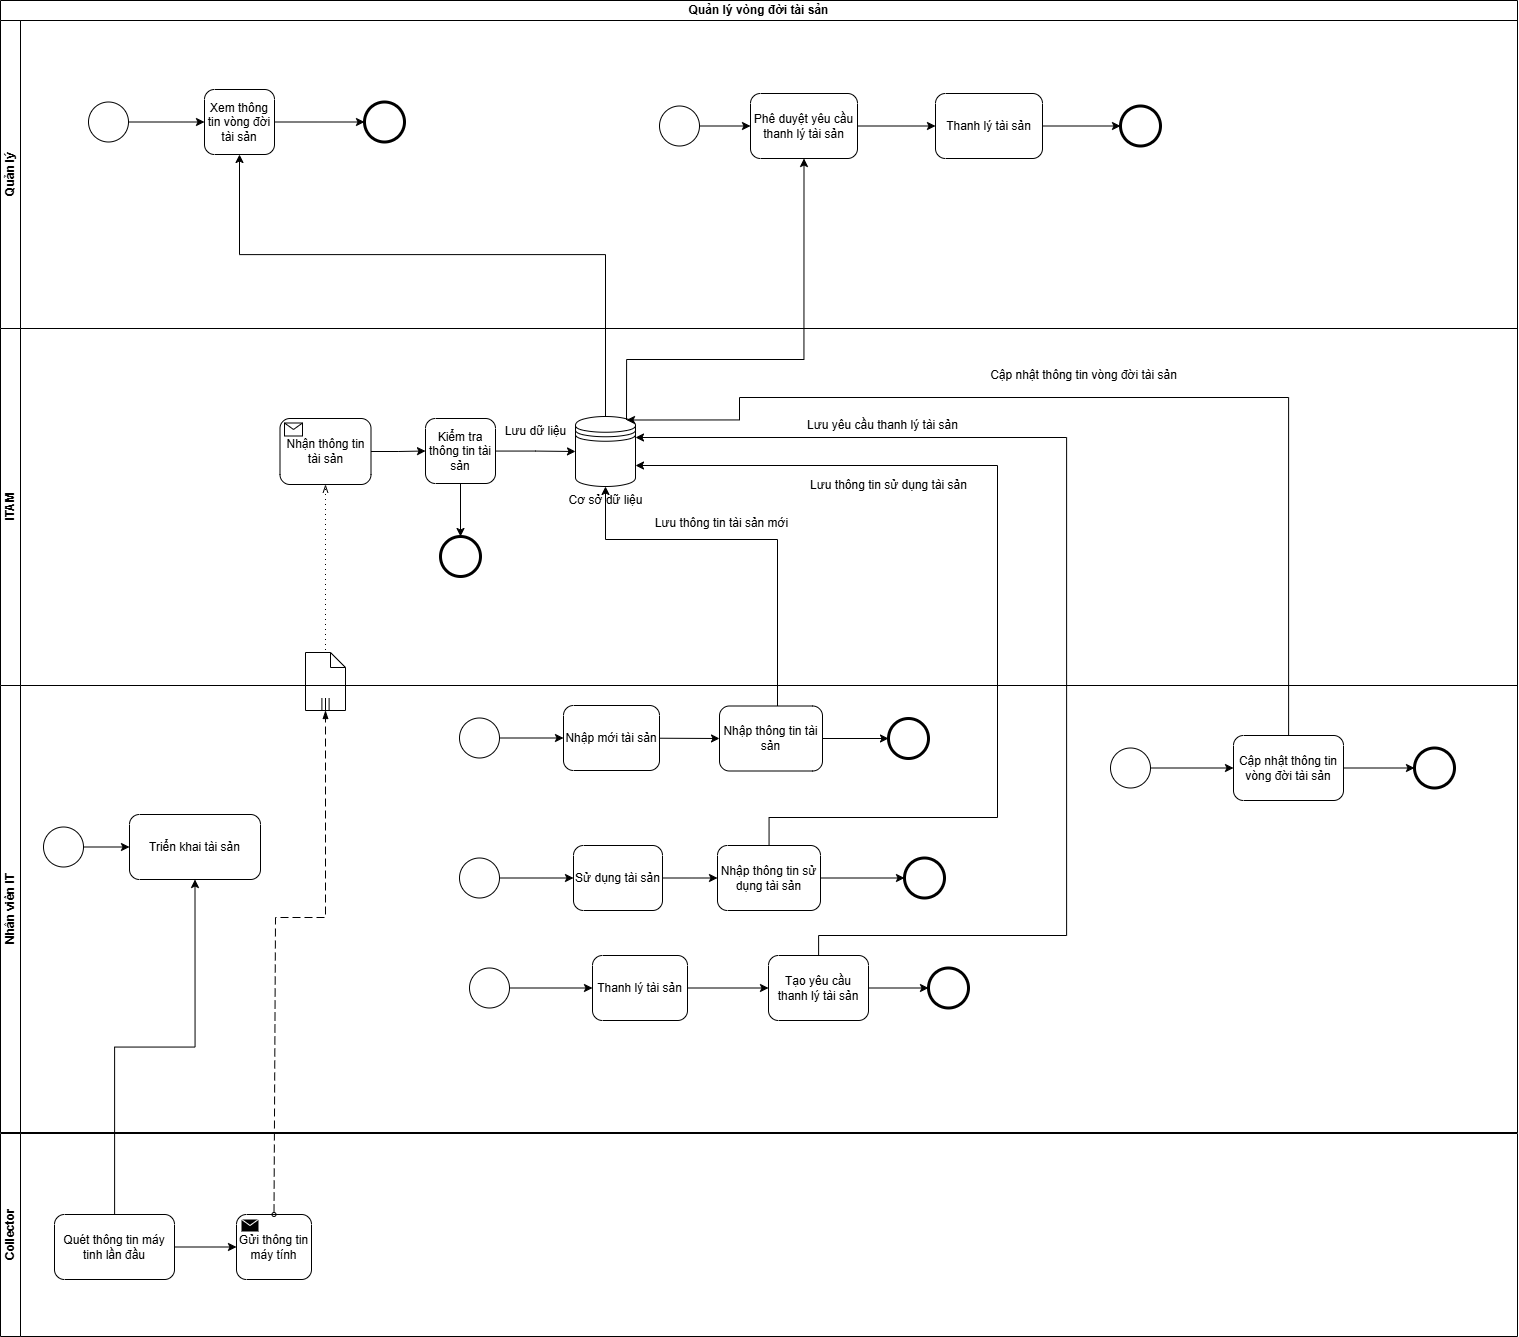
\includegraphics[width=\linewidth]{Images/C5/BPMN/RITAM-Quản lý vòng đời tài sản.drawio.png}
%     \vspace{15pt}
%     \caption{Mô hình hóa nghiệp vụ Quản lý vòng đời tài sản}
% \end{figure}
%     \begin{itemize}[label=--]
%        \item \textbf{Nhập mới tài sản:}
%        \begin{itemize}[label=\textbullet]
%            \item Sau khi hoàn tất giai đoạn mua sắm tài sản, Nhân viên IT nhận các thiết bị sẽ tiến hành nhập thông tin tài sản trên hệ thống.
%            \item Đối với các loại tài sản rời như Ổ cứng, Ram, card mạng, nhân viên có thể nhập trước các thông tin cơ bản. Tương tự đối với máy tính để bàn, máy tính Laptop, nhân viên IT nhập các thông tin cơ bản như hệ điều hành, mẫu mã, số seri.       
%        \end{itemize}
%        \item \textbf{Triển khai tài sản:}
%        \begin{itemize}[label=\textbullet]
%            \item Sau khi đã nhập xong thông tin, nhân viên IT tiến hành cài đặt tool và cấu hình lại để thu thập dữ liệu chi tiết phần cứng và phần mềm tại mỗi máy tính, rồi khởi động để bắt đầu quá trình thu thập dữ liệu lần đầu. 
%            \item Hệ thống tiếp nhận dữ liệu, kiểm tra dữ liệu và lưu dữ liệu chi tiết bao gồm dữ liệu về CPU, RAM, Ổ cứng, Card mạng, GPU (nếu có). 
%        \end{itemize}
%        \item \textbf{Sử dụng tài sản:}
%        \begin{itemize}[label=\textbullet]
%            \item Sau khi triển khai xong, nhân viên IT sẽ nhập thông tin sử dụng tài sản.
%            \item Hệ thống ghi nhận và cập nhật ở cơ sở dữ liệu.
%        \end{itemize}
%        \item \textbf{Thanh lý tài sản}:
%        \begin{itemize}[label=\textbullet]
%            \item Nhân viên tạo yêu cầu thanh lý tài sản.
%            \item Hệ thống ghi nhận và lưu lại cơ sở dữ liệu.
%            \item Quản lý sau đó có thể phê duyệt yêu cầu thanh lý tài sản. Hệ thống ghi nhận và lưu lại trạng thái đơn yêu cầu.
%            \item Sau khi đơn yêu cầu thanh lý đã được phê duyệt, nhân viên tiến hành thanh lý tài sản.
%        \end{itemize}
%     \end{itemize}
% %----------%
% %     \item Quản lý Dữ liệu Phần cứng và Phần mềm
% %      \begin{figure}[H]
% %     \centering
% %     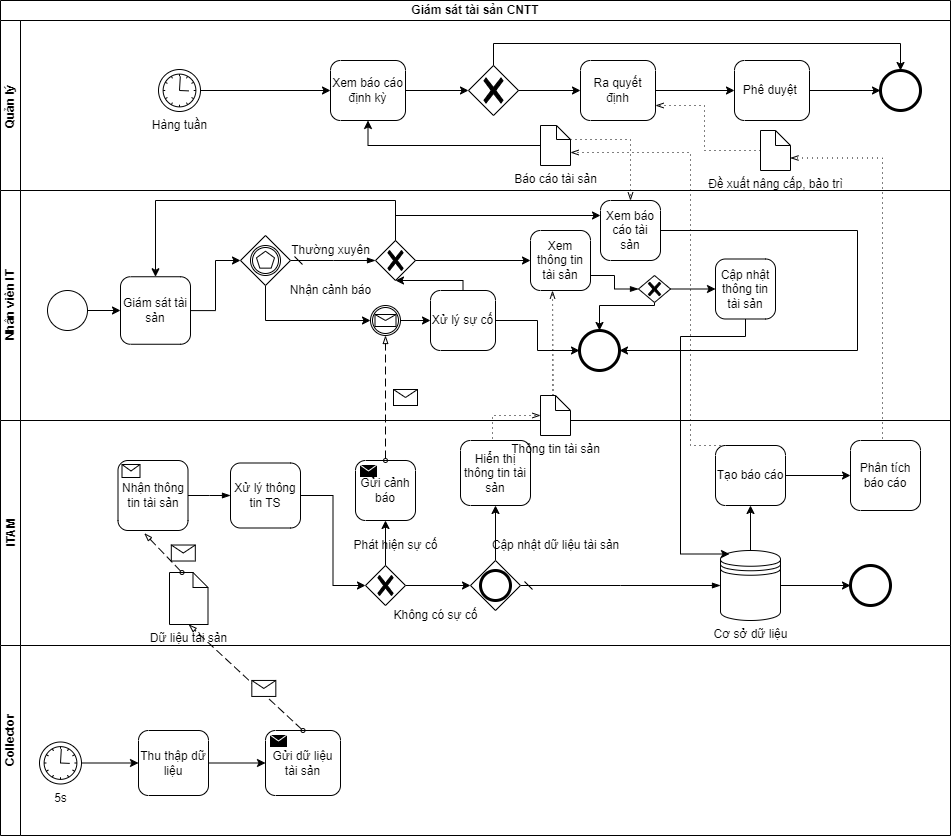
\includegraphics[width=\linewidth]{Images/C5/BPMN/BPMN-Giám sát Tài sản CNTT.png}
% %     \vspace{5pt}
% %     \caption{Mô hình hóa nghiệp vụ giám sát tài sản}
% % \end{figure}
%     \item \textbf{Cảnh báo}
%      \begin{figure}[H]
%     \centering
%     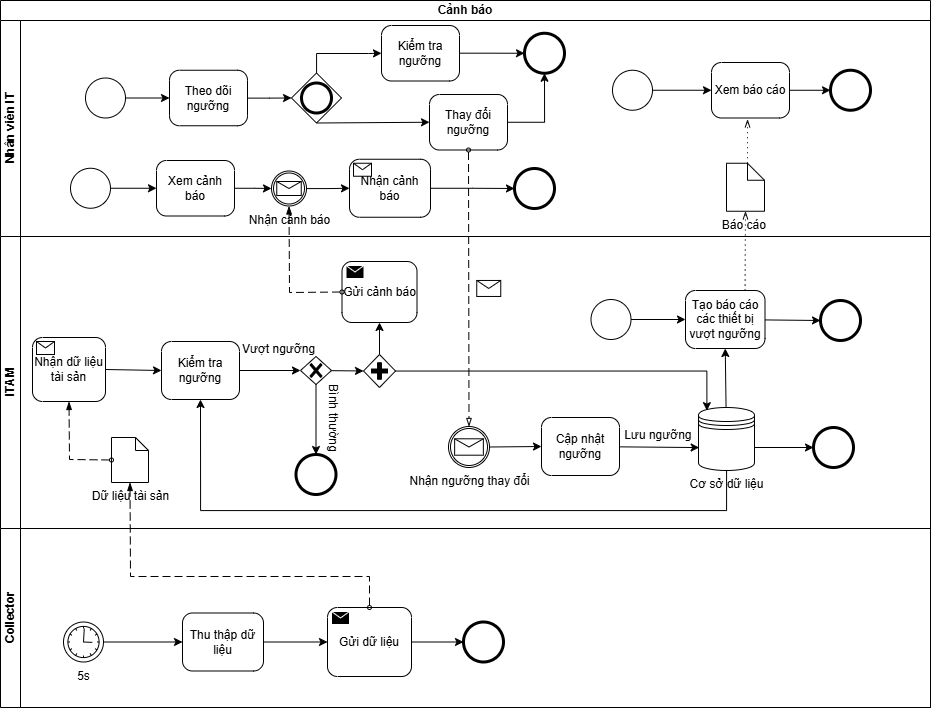
\includegraphics[width=\linewidth]{Images/C5/BPMN/BPMN-Cảnh báo.drawio.png}
%     \vspace{5pt}
%     \caption{Mô hình hóa nghiệp vụ Cảnh báo}
% \end{figure}
%     \begin{itemize}[label=--]
%         \item \textbf{Kiểm tra ngưỡng:}
%         \begin{itemize}[label=\textbullet]
%             \item Cứ 5 phút, Collector thu thập dữ liệu và gửi dữ liệu này đến hệ thống ITAM.
%             \item Hệ thống ITAM sau khi nhận dữ liệu sẽ kiểm tra thiết bị có vượt ngưỡng hay không. 
%             \item Nếu có tình trạng vượt ngưỡng, hệ thống sẽ gửi cảnh báo đến nhân viên IT phụ trách đồng thời lưu lại cảnh báo vào cơ sở dữ liệu. 
%             \item Nhân viên IT có thể xem các cảnh báo của các thiết bị vượt ngưỡng trên hệ thống.
%         \end{itemize}
%         \item \textbf{Theo dõi ngưỡng:}
%         \begin{itemize}[label=\textbullet]
%             \item Nhân viên IT có thể kiểm tra thông tin ngưỡng của các loại thiết bị.
%             \item Khi nhân viên thay đổi ngưỡng, hệ thống sẽ ghi nhận và thay đổi các chỉ số ở cơ sở dữ liệu.
%         \end{itemize}
%         \item \textbf{Báo cáo về các thiết bị vượt ngưỡng}
%         \begin{itemize}[label=\textbullet]
%             \item Khi nhân viên IT có nhu cầu xem báo cáo tổng quan về các thiết bị vượt ngưỡng, hệ thống sẽ tạo báo cáo từ cơ sở dữ liệu.
%         \end{itemize}
%     \end{itemize}
% %----------%
%     \item \textbf{Quản lý yêu cầu nâng cấp}
%     \begin{figure}[H]
%     \centering
%     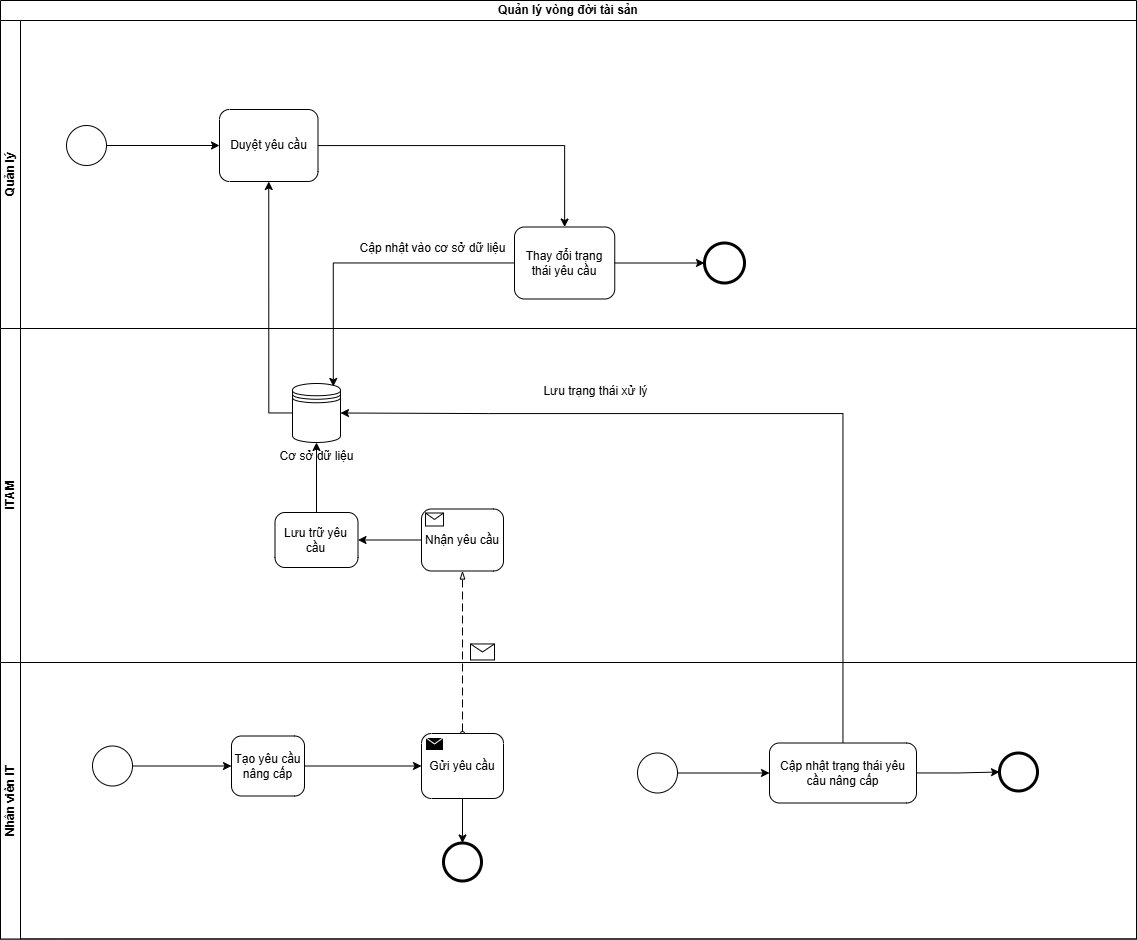
\includegraphics[width=0.8\linewidth]{Images/C5/BPMN/RITAM-Quản lý yêu cầu nâng cấp.drawio.png}
%     \vspace{10pt}
%     \caption{Mô hình hóa nghiệp vụ Quản lý yêu cầu nâng cấp tài sản}
% \end{figure}
%     \begin{itemize}[label=--]
%         \item Trong quá trình sử dụng tài sản, khi các thiết bị cũ cần được thay thế, nâng cấp, người dùng tài sản có thể báo cho nhân viên IT để tiến hành nâng cấp, thay thế tài sản.
%         \item Nhân viên khi nhận được yêu cầu từ người dùng tài sản sẽ tiến hành tạo yêu cầu nâng cấp tài sản.
%         \item Hệ thống sẽ lưu yêu cầu nâng cấp tài sản vào cơ sở dữ liệu và đợi phê duyệt từ quản lý.
%         \item Quản lý phê duyệt yêu cầu nâng cấp. Sau đó, hệ thống sẽ cập nhật trạng thái đã phê duyệt cho đơn yêu cầu nâng cấp.
%         \item Sau khi yêu cầu đã được phê duyệt thì nhân viên sẽ tiến hành nâng cấp hoặc thay thế tài sản. Khi hoàn thành nhân viên phải cập nhật trạng thái cho yêu cầu nâng cấp đã hoàn tất.
%         \item Khi hoàn tất yêu cầu nâng cấp, Tool sẽ tự động quét và gửi dữ liệu mới lên hệ thống. Hệ thống sau đó tiếp nhận và cập nhật thông tin vào cơ sở dữ liệu.
%     \end{itemize}
% %----------%    
%     \item \textbf{Quản lý sự cố và bảo trì}
%     \begin{figure}[H]
%     \centering
%     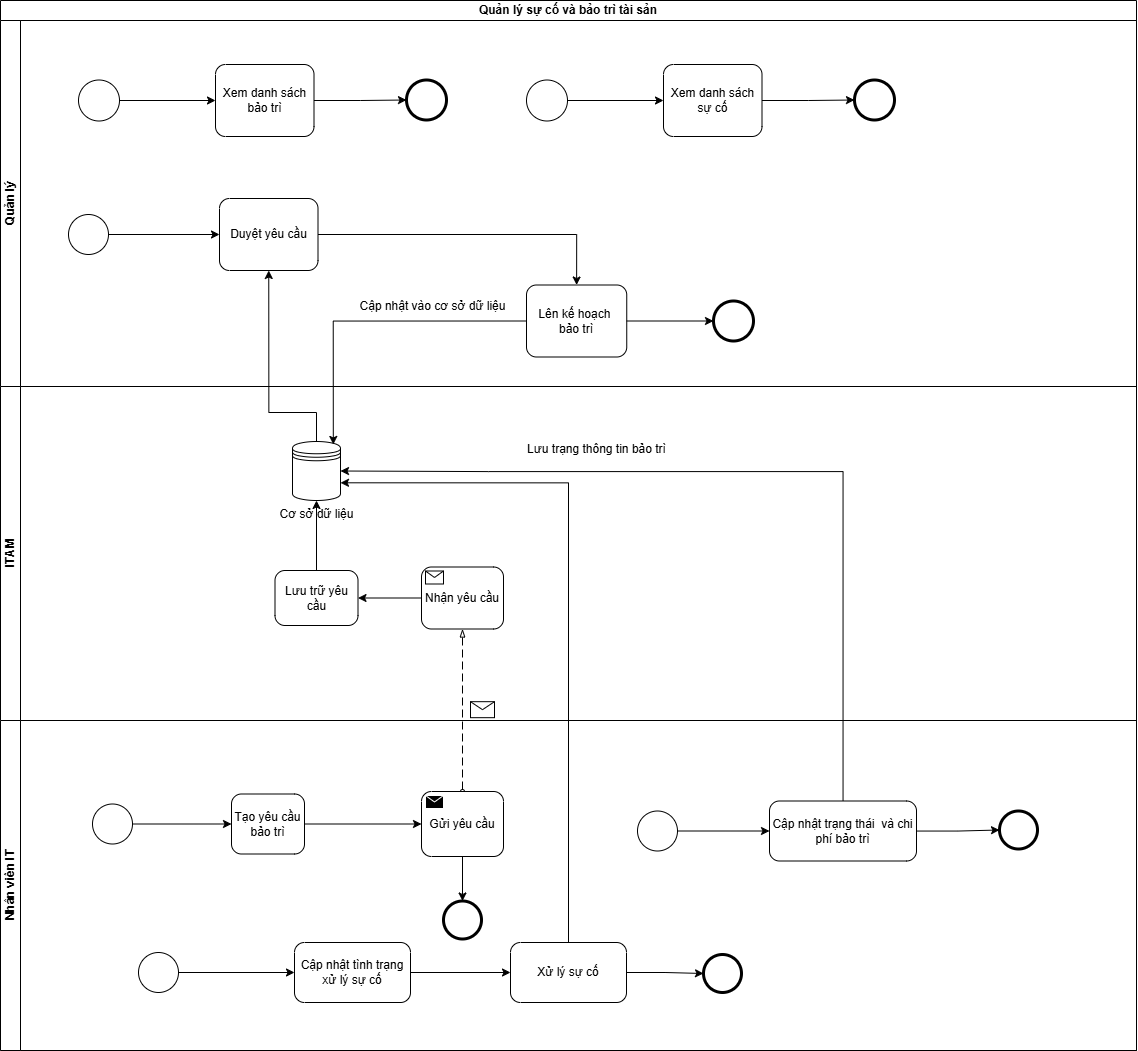
\includegraphics[width=0.8\linewidth]{Images/C5/BPMN/RITAM-Quản lý sự cố và bảo trì.drawio.png}
%     \vspace{10pt}
%     \caption{Mô hình hóa nghiệp vụ Quản lý sự cố và bảo trì tài sản}
% \end{figure}
%     \begin{itemize}[label=--]
%         \item \textbf{Quản lý sự cố tài sản}
%         \begin{itemize}[label=\textbullet]
%             \item Khi có sự cố tài sản, nhân viên IT sẽ lưu lại sự cố trên hệ thống và tiến hành xử lý sự cố.
%             \item Sau khi xử lý xong sự cố, nhân viên IT sẽ cập nhật trạng thái sự cố trên hệ thống.
%             \item Cả nhân viên IT và quản lý đều có thể xem lại lịch sử sự cố của từng máy.
%         \end{itemize}
%         \item \textbf{Quản lý bảo trì tài sản}
%         \begin{itemize}[label=\textbullet]
%             \item Nhân viên IT tạo yêu cầu bảo trì tài sản.
%             \item Hệ thống tiếp nhận và lưu yêu cầu bảo trì tài sản.
%             \item Quản lý phê duyệt yêu cầu bảo trì tài sản.
%             \item Nhân viên IT xác nhận thực hiện bảo trì, sau đó lên kế hoạch bảo trì tài sản.
%             \item Sau khi hoàn tất bảo trì tài sản, nhân viên IT cập nhật trạng thái và chi phí bảo trì.
%         \end{itemize}
%     \end{itemize}
% %----------%
%     \item \textbf{Quản lý Đơn đặt hàng}
%      \begin{figure}[H]
%     \centering
%     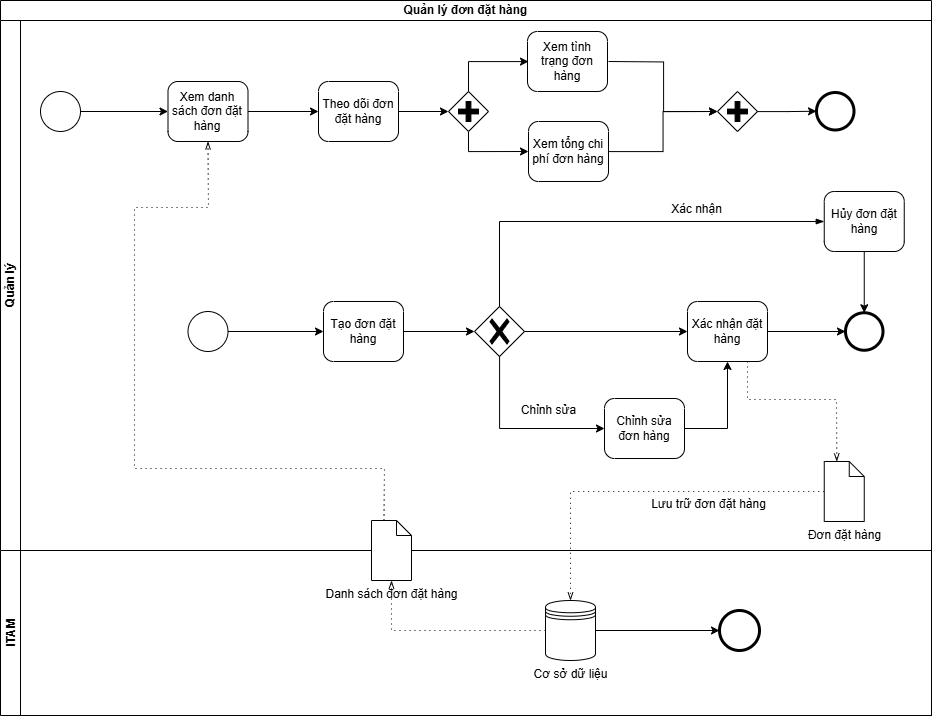
\includegraphics[width=\linewidth]{Images/C5/BPMN/RITAM-Quản lý đơn đặt hàng.drawio.png}
%     \vspace{5pt}
%     \caption{Mô hình hóa nghiệp vụ Quản lý đơn đặt hàng}
% \end{figure}
%     \begin{itemize}[label=--]
%         \item  \textbf{Tạo đơn đặt hàng:}
%         \begin{itemize}[label=\textbullet]
%             \item Quản lý tạo đơn đặt hàng trên hệ thống khi có nhu cầu mua sắm tài sản.
%             \item Sau khi tạo đơn hàng thì phải xác nhận đơn hàng, người tạo có thể chỉnh sửa rồi xác nhận lại đơn hàng. Quản lý phải gán mã nhân viên xử lý đơn hàng khi nhận hàng.
%             \item Đơn hàng sau khi xác nhận sẽ được lưu trữ vào cơ sở dữ liệu. 
%             \item Ngoài ra Quản lý có thể hủy đơn đặt hàng nếu trong quá trình tạo đơn có sai sót.
%         \end{itemize}
%         \item \textbf{Xem danh sách các đơn hàng:}
%         \begin{itemize}[label=\textbullet]
%             \item Quản lý có thể xem danh sách các đơn đặt hàng, họ có thể xem cụ thể một đơn hàng
%             \item Đơn hàng bao gồm các thông tin cơ bản, tình trạng và tổng chi phí cho đơn hàng ,thông tin nhân viên xử lý đơn hàng đó.
%         \end{itemize}
%     \end{itemize}
% %----------%
% \end{enumerate}

% \subsubsection{ Mô hình hóa tương tác}
% \begin{itemize}[label=--]
% \item{Use case toàn hệ thống}
% \begin{figure}[H]
%     \centering
%     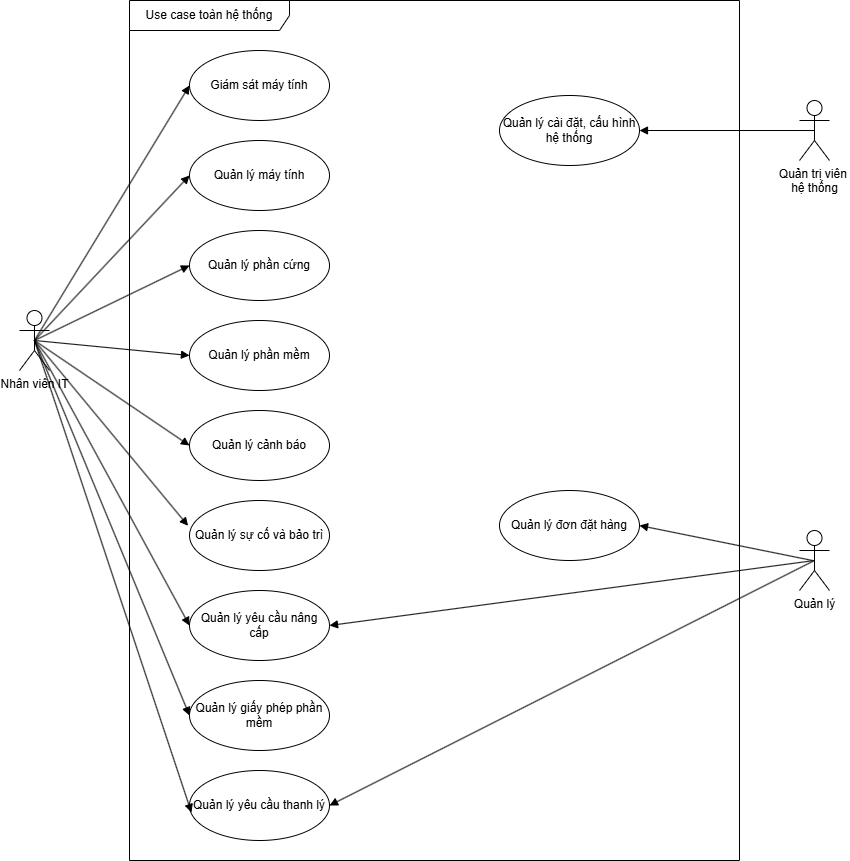
\includegraphics[width=\linewidth]{Images/C5/UseCaseDiagrams/Use-case-General.drawio.png}
%     \vspace{5pt}
%     \caption{Use case toàn hệ thống}
% \end{figure}

% % \subsubsubsection{ Use case Đăng nhập}
% % \begin{figure}[H]
% %     \centering
% %     \includegraphics[width=\linewidth]{Images/C5/UseCaseDiagrams/Use-case-Dang-nhap.drawio.png}
% %     \vspace{5pt}
% %     \caption{Use case Đăng nhập}
% % \end{figure}
% %%----------------------------------
% % \begin{table}[H]
% %         \centering
% %         \begin{tabular}{|p{4cm}|p{10cm}|}
% %             \hline
% %             Tên use-case & Đăng nhập\\
% %             \hline
% %             Đối tượng & Nhân viên IT, Quản lý, Quản trị viên hệ thống \\
% %             \hline
% %             Mô tả & Nhân viên IT, Quản lý, Quản trị viên hệ thống thực hiện đăng nhập vào hệ thống ITAM \\
% %             \hline
% %             Diều kiện kích hoạt &  Nhân viên IT, Quản lý, Quản trị viên hệ thống bấm vào mục "Đăng nhập"\\
% %             \hline
% %             Tiền điều kiện & Nhân viên IT, Quản lý, Quản trị viên hệ thống chưa đăng nhập vào hệ thống, đã có tài khoản và mật khẩu \\
% %             \hline
% %             Hậu điều kiện & Nhân viên IT, Quản lý, Quản trị viên hệ thống đăng nhập vào hệ thống thành công \\
% %             \hline
% %             Luồng tương tác chính & 
% %             \begin{enumerate}
% %                 \item Nhân viên IT, Quản lý, Quản trị viên hệ thống truy cập vào màn hình đăng nhập.
% %                 \item Nhân viên IT, Quản lý, Quản trị viên hệ thống điền thông tin tài khoản và mật khẩu.
% %                 \item Nếu thông tin đăng nhập đúng và chính xác, Nhân viên IT, Quản lý, Quản trị viên hệ thống đăng nhập vào hệ thống và chuyển đến trang chủ.
% %             \end{enumerate}\\
% %             \hline
% %             % Luồng tương tác thay thế& b \\
% %             % \hline
% %             Luồng tương tác ngoại lệ & Nếu trong quá trình xác thực tài khoản có vấn đề hay lỗi thì hệ thống sẽ trả về lỗi tài khoản chưa được xác thực thành công. Nếu tài khoản không tồn tại hệ thống trả về lỗi không tồn tại tài khoản. Nếu sai mật khẩu hệ thống trả về lỗi sai mật khẩu \\
% %             \hline
% %         \end{tabular}
% %         \caption{Đặc tả Use case Đăng nhập}
% %         \label{tab:my_label}
% % oi\end{table}

% \item{ Use case Giám sát máy tính}
% \begin{figure}[H]
%     \centering
%     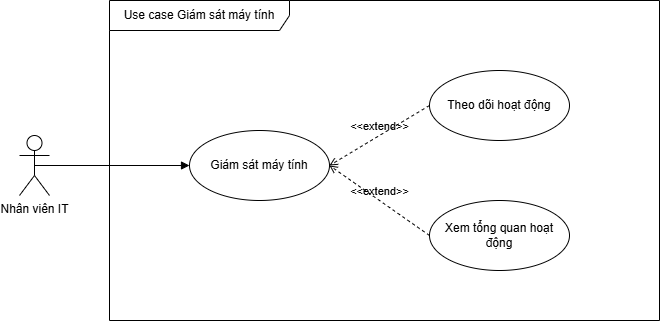
\includegraphics[width=\linewidth]{Images/C5/UseCaseDiagrams/Use-case-Giam-sat-may-tinh.drawio.png}
%     \vspace{5pt}
%     \caption{Use case Giám sát máy tính}
% \end{figure}

% \begin{table}[H]
%     \centering
%     \caption{Đặc tả Use case Giám sát máy tính}
%     \begin{tabular}{|p{4cm}|p{10cm}|}
%         \hline
%         Tên use-case & Giám sát máy tính\\
%         \hline
%         Đối tượng & Nhân viên IT \\
%         \hline
%         Mô tả & Nhân viên IT có thể giám sát hoạt động của máy tính, bao gồm theo dõi hoạt động và xem tổng quan hoạt động. \\
%         \hline
%         Điều kiện kích hoạt & Nhân viên IT chọn vào mục "Giám sát máy tính" trên giao diện hệ thống.\\
%         \hline
%         Tiền điều kiện & 
%         \begin{itemize}
%             \item Nhân viên IT đã đăng nhập vào hệ thống.
%             \item Nhân viên IT có quyền truy cập tính năng giám sát máy tính.
%         \end{itemize}\\
%         \hline
%         Hậu điều kiện & Nhân viên IT giám sát thành công các hoạt động của máy tính. \\
%         \hline
%         Luồng tương tác chính &
%         \begin{enumerate}
%             \item Nhân viên IT truy cập vào mục "Giám sát máy tính".
%             \item Nhân viên IT chọn "Hoạt động" để xem giao diện giám sát máy tính.
%             \item Hệ thống hiển thị giao diện giám sát máy tính theo thời gian thực.
%         \end{enumerate}\\
%         \hline
%         Luồng tương tác thay thế&
%         Tại bước 2:
%         \newline
%             2.1. Nhân viên IT chọn "Tổng quan hoạt động" để xem tổng quan hoạt động của các máy tính trong hệ thống.
%         \newline 
%             2.2. Hệ thống hiển thị giao diện tổng quan hoạt động của các máy tính trong hệ thống.
%         \\
%         \hline
%         Luồng tương tác ngoại lệ & 
%         Tại bước 3: Hệ thống lỗi khi hiển thị giao diện giám sát theo thời gian thực, hệ thống báo lỗi.
%         \newline
%         Tại bước 2.2: Hệ thống lỗi khi hiển thị tổng quan hoạt động của các máy tính, hệ thống báo lỗi.
%         \\
%         \hline
%     \end{tabular}
    
%     \label{tab:use_case_monitor}
% \end{table}


% \item{ Use case Quản lý máy tính}
% \begin{figure}[H]
%     \centering
%     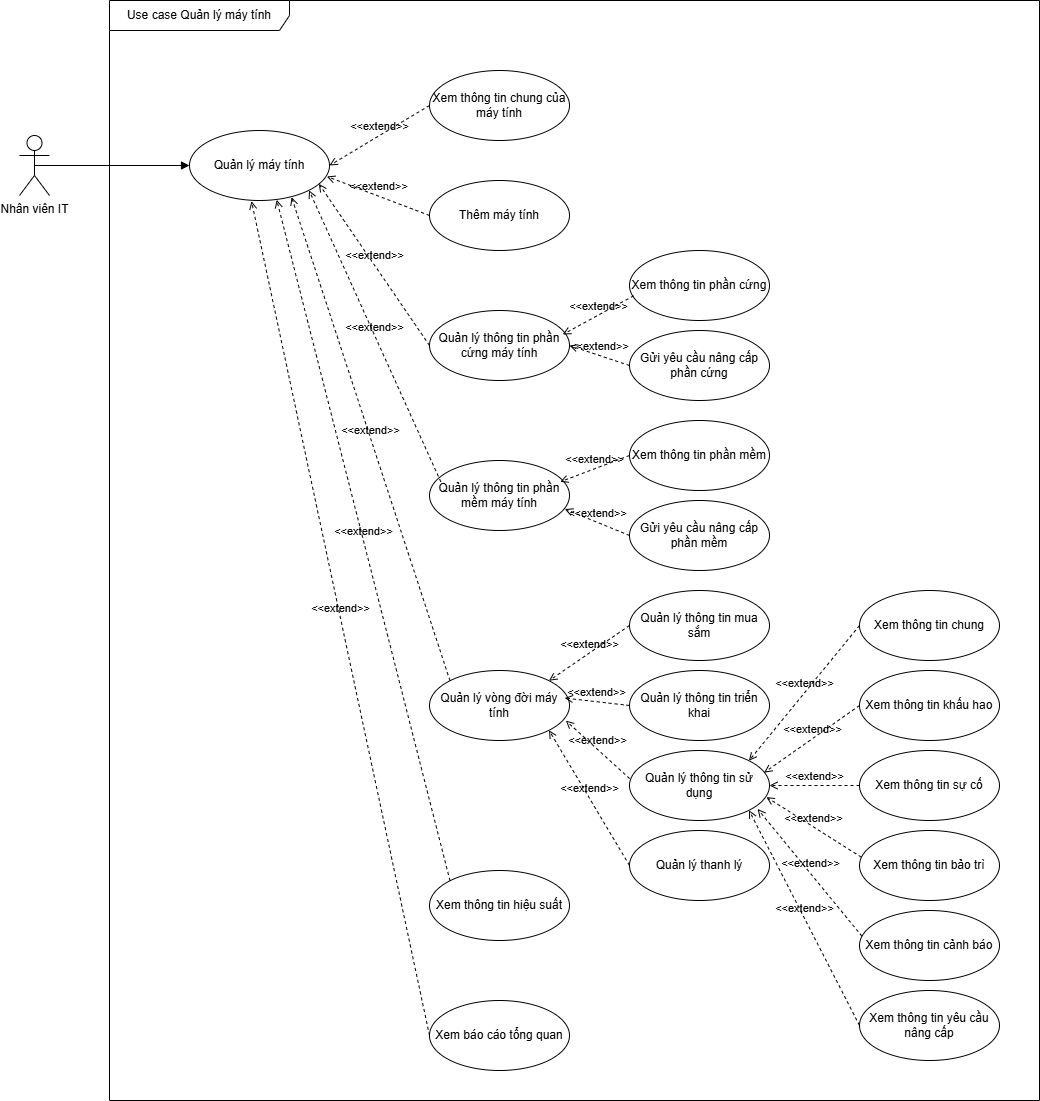
\includegraphics[width=\linewidth]{Images/C5/UseCaseDiagrams/Use-case-Quan-ly-may-tinh.drawio.png}
%     \vspace{5pt}
%     \caption{Use case Quản lý máy tính}
% \end{figure}

% \begin{table}[H]
%         \centering
%         \caption{Đặc tả Use case Xem thông tin chung của máy tính}
%         \begin{tabular}{|p{4cm}|p{10cm}|}
%             \hline
%             Tên use-case & Xem thông tin chung của máy tính\\
%             \hline
%             Đối tượng & Nhân viên IT \\
%             \hline
%             Mô tả & Nhân viên IT có thể thực hiện xem thông tin chung của máy tính \\
%             \hline
%             Diều kiện kích hoạt & Nhân viên IT chọn máy tính cần xem thông tin \\
%             \hline
%             Tiền điều kiện & Nhân viên IT đã đăng nhập vào hệ thống, có quyền truy cập vào tính năng Quản lý máy tính. \\
%             \hline
%             Hậu điều kiện & Nhân viên IT có thể thực hiện xem thông tin chung của máy tính thành công \\
%             \hline
%             Luồng tương tác chính &
%             \begin{enumerate}
%                 \item Nhân viên IT chọn "Quản lý máy tính" ở giao diện chính của hệ thống.
%                 \item Hệ thống hiển thị danh sách các máy tính.
%                 \item Nhân viên IT chọn máy tính cần xem thông tin từ danh sách.
%                 \item Hệ thống hiện thị thông tin về máy tính đã chọn.
%             \end{enumerate}\\
%             \hline
%             Luồng tương tác thay thế&  
%             Không có\\
%             \hline
%             Luồng tương tác ngoại lệ & 
%             Tại bước 2: Hệ thống lỗi trong việc hiển thị danh sách các máy tính, hệ thống báo lỗi.
            
%             Tại bước 4: Hệ thống lỗi trong việc hiển thị thông tin máy tính, hệ thống báo lỗi.
%             \\
%             \hline
%         \end{tabular}
        
%         \label{tab:my_label}
% \end{table}

% \begin{table}[H]
%         \centering
%         \caption{Đặc tả Use case Thêm máy tính}
%         \begin{tabular}{|p{4cm}|p{10cm}|}
%             \hline
%             Tên use-case & Thêm máy tính\\
%             \hline
%             Đối tượng & Nhân viên IT \\
%             \hline
%             Mô tả & Nhân viên IT có thể thực hiện thêm máy tính \\
%             \hline
%             Diều kiện kích hoạt & Nhân viên IT chọn "Thêm máy tính" \\
%             \hline
%             Tiền điều kiện & Nhân viên IT đã đăng nhập vào hệ thống, có quyền truy cập vào tính năng Quản lý máy tính. \\
%             \hline
%             Hậu điều kiện & Nhân viên IT có thể thực hiện thêm máy tính thành công \\
%             \hline
%             Luồng tương tác chính &
%             \begin{enumerate}
%                 \item Nhân viên IT chọn "Quản lý máy tính" ở giao diện chính của hệ thống.
%                 \item Hệ thống hiển thị danh sách các máy tính và nút "Thêm máy tính"
%                 \item Nhân viên IT chọn nút "Thêm máy tính".
%                 \item Hệ thống hiện thị trang biểu mẫu thêm máy tính.
%                 \item Nhân viên IT thực hiện điền thông tin máy tính cần thêm mới và nhấn nút "Lưu".
%                 \item Hệ thống kiểm tra và ghi nhận thông tin máy tính mới và báo thành công.
%             \end{enumerate}\\
%             \hline
%             Luồng tương tác thay thế&  
%             Tại bước 5: Nếu muốn hủy bỏ thêm máy tính, Nhân viên IT bấm "Trở về". Tiếp tục bước 2\\
%             \hline
%             Luồng tương tác ngoại lệ & 
%             Tại bước 2: Hệ thống lỗi trong việc hiển thị danh sách các máy tính, hệ thống báo lỗi.
            
%             Tại bước 4: Hệ thống lỗi trong việc kiểm tra và ghi nhận thông tin máy tính mới, hệ thống báo lỗi.

%             Tại bước 4: Hệ thống kiểm tra thông tin máy tính mới và không cho phép lưu, hệ thống báo lỗi cho người dùng.
%             \\
%             \hline
%         \end{tabular}
        
%         \label{tab:my_label}
% \end{table}

% \begin{table}[H]
%         \centering
%         \caption{Đặc tả Use case Quản lý thông tin phần cứng máy tính}
%         \begin{tabular}{|p{4cm}|p{10cm}|}
%             \hline
%             Tên use-case & Quản lý thông tin phần cứng máy tính\\
%             \hline
%             Đối tượng & Nhân viên IT \\
%             \hline
%             Mô tả & Nhân viên IT có thể thực hiện quản lý thông tin phần cứng máy tính \\
%             \hline
%             Diều kiện kích hoạt & Nhân viên IT chọn "Thông tin phần cứng" \\
%             \hline
%             Tiền điều kiện & Nhân viên IT đã đăng nhập vào hệ thống, có quyền truy cập vào tính năng Quản lý máy tính. \\
%             \hline
%             Hậu điều kiện & Nhân viên IT có thể thực hiện quản lý thông tin phần cứng máy tính thành công \\
%             \hline
%             Luồng tương tác chính &
%             \begin{enumerate}
%                 \item Nhân viên IT chọn "Quản lý máy tính" ở giao diện chính của hệ thống.
%                 \item Hệ thống hiển thị danh sách các máy tính.
%                 \item Nhân viên IT chọn máy tính cần quản lý.
%                 \item Hệ thống hiện thị thông tin chi tiết của máy tính.
%                 \item Nhân viên IT chọn nút "Thông tin phần cứng"
%                 \item Hệ thống hiển thị thông tin về phần cứng máy tính và nút "Gửi yêu cầu nâng cấp".
%                 \item Nhân viên IT chọn nút "Gửi yêu cầu nâng cấp".
%                 \item Hệ thống xuất hiện biểu mẫu "Yêu cầu nâng cấp".
%                 \item Nhân viên IT điền vào biểu mẫu và nhấn nút "Gửi".
%                 \item Hệ thống kiểm tra và lưu yêu cầu nâng cấp.
%             \end{enumerate}\\
%             \hline
%             Luồng tương tác thay thế&  
%             Tại bước 6: Nhân viên IT bấm "Trở về". Tiếp tục bước 2

%             Tại bước 9: Nếu muốn hủy bỏ yêu cầu nâng cấp phần cứng, bấm "Hủy".
%             \\
%             \hline
%             Luồng tương tác ngoại lệ & 
%             Tại bước 2: Hệ thống lỗi trong việc hiển thị danh sách các máy tính, hệ thống báo lỗi.

%             Tại bước 6: Hệ thống lỗi trong việc hiển thị thông tin phần cứng, hệ thống báo lỗi.
            
%             Tại bước 10: Hệ thống lỗi trong việc kiểm tra và ghi nhận yêu cầu nâng cấp, hệ thống báo lỗi.

%             Tại bước 10: Hệ thống kiểm tra yêu cầu nâng cấp và không cho phép lưu, hệ thống báo lỗi cho người dùng.
%             \\
%             \hline
%         \end{tabular}
        
%         \label{tab:my_label}
% \end{table}

% \begin{table}[H]
%         \centering\
%         \caption{Đặc tả Use case Quản lý thông tin phần mềm máy tính}
%         \begin{tabular}{|p{4cm}|p{10cm}|}
%             \hline
%             Tên use-case & Quản lý thông tin phần mềm máy tính\\
%             \hline
%             Đối tượng & Nhân viên IT \\
%             \hline
%             Mô tả & Nhân viên IT có thể thực hiện quản lý thông tin phần mềm máy tính \\
%             \hline
%             Diều kiện kích hoạt & Nhân viên IT chọn "Thông tin phần mềm" \\
%             \hline
%             Tiền điều kiện & Nhân viên IT đã đăng nhập vào hệ thống, có quyền truy cập vào tính năng Quản lý máy tính. \\
%             \hline
%             Hậu điều kiện & Nhân viên IT có thể thực hiện quản lý thông tin phần mềm máy tính thành công \\
%             \hline
%             Luồng tương tác chính &
%             \begin{enumerate}
%                 \item Nhân viên IT chọn "Quản lý máy tính" ở giao diện chính của hệ thống.
%                 \item Hệ thống hiển thị danh sách các máy tính.
%                 \item Nhân viên IT chọn máy tính cần quản lý.
%                 \item Hệ thống hiện thị thông tin chi tiết của máy tính.
%                 \item Nhân viên IT chọn nút "Thông tin phần mềm"
%                 \item Hệ thống hiển thị danh sách thông tin về phần mềm máy tính và nút "Gửi yêu cầu nâng cấp".
%                 \item Nhân viên IT chọn nút "Gửi yêu cầu nâng cấp".
%                 \item Hệ thống xuất hiện biểu mẫu "Yêu cầu nâng cấp".
%                 \item Nhân viên IT điền vào biểu mẫu và nhấn nút "Gửi".
%                 \item Hệ thống kiểm tra và lưu yêu cầu nâng cấp.
%             \end{enumerate}\\
%             \hline
%             Luồng tương tác thay thế&  
%             Tại bước 6: Nhân viên IT bấm "Trở về". Tiếp tục bước 2

%             Tại bước 9: Nếu muốn hủy bỏ yêu cầu nâng cấp phần mềm, bấm "Hủy".
%             \\
%             \hline
%             Luồng tương tác ngoại lệ & 
%             Tại bước 2: Hệ thống lỗi trong việc hiển thị danh sách các máy tính, hệ thống báo lỗi.

%             Tại bước 6: Hệ thống lỗi trong việc hiển thị danh sách thông tin phần mềm, hệ thống báo lỗi.
            
%             Tại bước 10: Hệ thống lỗi trong việc kiểm tra và ghi nhận yêu cầu nâng cấp, hệ thống báo lỗi.

%             Tại bước 10: Hệ thống kiểm tra yêu cầu nâng cấp và không cho phép lưu, hệ thống báo lỗi cho người dùng.
%             \\
%             \hline
%         \end{tabular}
        
%         \label{tab:my_label}
% \end{table}

% \begin{table}[H]
%         \centering
%         \caption{Đặc tả Use case Quản lý vòng đời máy tính}
%         \begin{tabular}{|p{4cm}|p{10cm}|}
%             \hline
%             Tên use-case & Quản lý vòng đời máy tính\\
%             \hline
%             Đối tượng & Nhân viên IT \\
%             \hline
%             Mô tả & Nhân viên IT có thể thực hiện quản lý vòng đời máy tính \\
%             \hline
%             Diều kiện kích hoạt & Nhân viên IT chọn "Vòng đời tài sản" \\
%             \hline
%             Tiền điều kiện & Nhân viên IT đã đăng nhập vào hệ thống, có quyền truy cập vào tính năng Quản lý máy tính. \\
%             \hline
%             Hậu điều kiện & Nhân viên IT có thể thực hiện quản lý vòng đời máy tính thành công \\
%             \hline
%             Luồng tương tác chính &
%             \begin{enumerate}
%                 \item Nhân viên IT chọn "Quản lý máy tính" ở giao diện chính của hệ thống.
%                 \item Hệ thống hiển thị danh sách các máy tính.
%                 \item Nhân viên IT chọn máy tính cần quản lý.
%                 \item Hệ thống hiện thị thông tin chi tiết của máy tính.
%                 \item Nhân viên IT chọn nút "Vòng đời tài sản"
%                 \item Nhân viên IT chọn nút "Mua sắm"
%                 \item Hệ thống hiển thị thông tin về mua sắm tài sản.
%             \end{enumerate}\\
%             \hline
%             Luồng tương tác thay thế&  
%             Tại bước 6:
            
%             6.1.1. Nhân viên IT chọn "Triển khai".
            
%             6.1.2. Hệ thống hiển thị thông tin về triển khai máy tính.
            

%             Tại bước 6:
            
%             6.2.1. Nhân viên IT chọn "Sử dụng".
            
%             6.2.2. Hệ thống hiển thị thông tin về sử dụng máy tính bao gồm thông tin chung về sử dụng, thông tin khấu hao, thông tin về sự cố máy tính, thông tin về bảo trì, thông tin về cảnh báo, thông tin về yêu cầu nâng cấp của máy tính.


%             Tại bước 6:
            
%             6.3.1. Nhân viên IT chọn "Thanh lý".
            
%             6.3.2. Hệ thống hiển thị thông tin về thanh lý máy tính.

%             \\
%             \hline
%             Luồng tương tác ngoại lệ & 
%             Tại bước 2: Hệ thống lỗi trong việc hiển thị danh sách các máy tính, hệ thống báo lỗi.

%             Tại bước 7, 6.1.2, 6.2.2, 6.3.2: Hệ thống lỗi trong việc hiển thị thông tin, hệ thống báo lỗi.
%             \\
%             \hline
%         \end{tabular}
        
%         \label{tab:my_label}
% \end{table}

% \begin{table}[H]
%         \centering
%         \caption{Đặc tả Use case Xem thông tin hiệu suất}
%         \begin{tabular}{|p{4cm}|p{10cm}|}
%             \hline
%             Tên use-case & Xem thông tin hiệu suất\\
%             \hline
%             Đối tượng & Nhân viên IT \\
%             \hline
%             Mô tả & Nhân viên IT có thể thực hiện xem thông tin hiệu suất máy tính \\
%             \hline
%             Diều kiện kích hoạt & Nhân viên IT chọn "Hiệu suất máy tính" \\
%             \hline
%             Tiền điều kiện & Nhân viên IT đã đăng nhập vào hệ thống, có quyền truy cập vào tính năng Quản lý máy tính. \\
%             \hline
%             Hậu điều kiện & Nhân viên IT có thể thực hiện xem thông tin hiệu suất thành công \\
%             \hline
%             Luồng tương tác chính &
%             \begin{enumerate}
%                 \item Nhân viên IT chọn "Quản lý máy tính" ở giao diện chính của hệ thống.
%                 \item Hệ thống hiển thị danh sách các máy tính.
%                 \item Nhân viên IT chọn máy tính cần quản lý.
%                 \item Hệ thống hiện thị thông tin chi tiết của máy tính.
%                 \item Nhân viên IT chọn nút "Hiệu suất máy tính"
%                 \item Hệ thống hiển thị thông tin về hiệu suất máy tính.
%             \end{enumerate}\\
%             \hline
%             Luồng tương tác thay thế&  
%             Tại bước 6: Nhân viên IT bấm "Trở về". Tiếp tục bước 2
%             \\
%             \hline
%             Luồng tương tác ngoại lệ & 
%             Tại bước 2: Hệ thống lỗi trong việc hiển thị danh sách các máy tính, hệ thống báo lỗi.

%             Tại bước 6: Hệ thống lỗi trong việc hiển thị hiệu suất, hệ thống báo lỗi.
%             \\
%             \hline
%         \end{tabular}
        
%         \label{tab:my_label}
% \end{table}

% \begin{table}[H]
%         \centering
%         \caption{Đặc tả Use case Xem báo cáo tổng quan}
%         \begin{tabular}{|p{4cm}|p{10cm}|}
%             \hline
%             Tên use-case & Xem báo cáo tổng quan\\
%             \hline
%             Đối tượng & Nhân viên IT \\
%             \hline
%             Mô tả & Nhân viên IT có thể thực hiện xem báo cáo tổng quan của các máy tính \\
%             \hline
%             Diều kiện kích hoạt & Nhân viên IT chọn "Báo cáo tổng quan" \\
%             \hline
%             Tiền điều kiện & Nhân viên IT đã đăng nhập vào hệ thống, có quyền truy cập vào tính năng Quản lý máy tính. \\
%             \hline
%             Hậu điều kiện & Nhân viên IT có thể thực hiện xem báo cáo tổng quan các máy tính thành công \\
%             \hline
%             Luồng tương tác chính &
%             \begin{enumerate}
%                 \item Nhân viên IT chọn "Quản lý máy tính" ở giao diện chính của hệ thống.
%                 \item Hệ thống hiển thị danh sách các máy tính.
%                 \item Nhân viên IT chọn "Báo cáo tổng quan".
%                 \item Hệ thống hiện thị báo cáo tổng quan về các máy tính.
%             \end{enumerate}\\
%             \hline
%             Luồng tương tác thay thế&  
%             Không có\\
%             \hline
%             Luồng tương tác ngoại lệ & 
%             Tại bước 2: Hệ thống lỗi trong việc hiển thị danh sách các máy tính, hệ thống báo lỗi.
            
%             Tại bước 4: Hệ thống lỗi trong việc hiển thị báo cáo tổng quan các máy tính, hệ thống báo lỗi.
%             \\
%             \hline
%         \end{tabular}
        
%         \label{tab:my_label}
% \end{table}

% \item{ Use case Quản lý phần cứng}
% \begin{figure}[H]
%     \centering
%     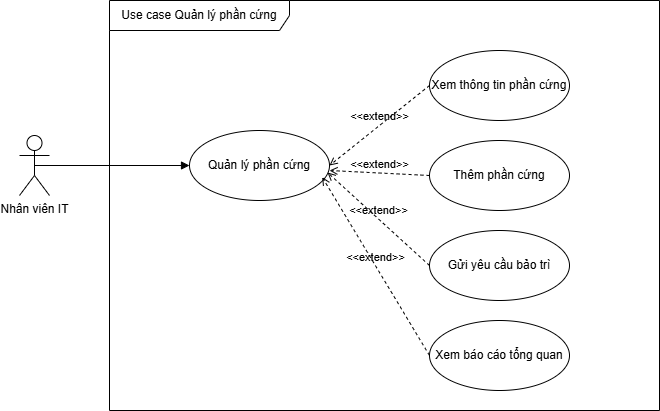
\includegraphics[width=\linewidth]{Images/C5/UseCaseDiagrams/Use-case-Quan-ly-phan-cung.drawio.png}
%     \vspace{5pt}
%     \caption{Use case Quản lý phần cứng}
% \end{figure}
% \begin{table}[H]
%         \centering
%         \caption{Đặc tả Use case Quản lý phần cứng}
%         \begin{tabular}{|p{4cm}|p{10cm}|}
%             \hline
%             Tên use-case & Quản lý phần cứng\\
%             \hline
%             Đối tượng & Nhân viên IT \\
%             \hline
%             Mô tả & Nhân viên IT thực hiện quản lý phần cứng \\
%             \hline
%             Diều kiện kích hoạt & Nhân viên IT bấm nút "Phần cứng" trên giao diện chính của hệ thống \\
%             \hline
%             Tiền điều kiện & Nhân viên IT đã đăng nhập vào hệ thống, có quyền truy cập vào tính năng Quản lý phần cứng. \\
%             \hline
%             Hậu điều kiện & Nhân viên IT thực hiện quản lý phần cứng thành công. \\
%             \hline
%             Luồng tương tác chính & 
%             \begin{enumerate}
%                 \item Nhân viên IT chọn "Phần cứng" ở giao diện chính của hệ thống.
%                 \item Hệ thống hiển thị danh sách các phần cứng.
%                 \item Nhân viên IT chọn phần cứng cần xem chi tiết.
%                 \item Hệ thống hiển thị thông tin chi tiết của phần cứng.
%             \end{enumerate}
%             \\
%             \hline
%             Luồng tương tác thay thế&
            
%             Tại bước 3:
            
%             3.1. Nhân viên IT chọn "Thêm phần cứng" để thêm phần cứng mới.
            
%             3.2. Hệ thống hiển thị giao diện thêm phần cứng.
            
%             3.3. Nhân viên IT nhập thông tin cho phần cứng cần thêm và bấm "Lưu".

%             3.4. Hệ thống kiểm tra và ghi nhận thông tin phần cứng.
%             \newline

%             Tại bước 4:
            
%             4.1. Nhân viên IT chọn "Gửi yêu cầu bảo trì".
            
%             4.2. Hệ thống hiển thị biểu mẫu yêu cầu bảo trì cho phần cứng.
            
%             4.3. Nhân viên IT nhập thông tin bảo trì.

%             4.4. Hệ thống kiểm tra và ghi nhận thông tin bảo trì.
%             \newline

%             Tại bước 2:
            
%             2.1. Nhân viên IT chọn "Báo cáo tổng quan".
            
%             2.2. Hệ thống hiển thị báo cáo tổng quan về phần cứng.
%             \\
%             \hline
%             Luồng tương tác ngoại lệ &
            
%             Tại bước 2: Hệ thống lỗi trong việc hiển thị danh sách phần cứng, hệ thống báo lỗi.

%             Tại bước 4: Hệ thống lỗi trong việc hiển thị thông tin phần cứng, hệ thống báo lỗi.

%             Tại bước 2.2: Hệ thống lỗi trong việc hiển thị báo cáo thổng quan về phần cứng, hệ thống báo lỗi.

%             Tại bước 3.4: Hệ thống lỗi trong việc kiểm tra và ghi nhận thông tin phần cứng, hệ thống báo lỗi.

%             Tại bước 4.4: Hệ thống lỗi trong việc kiểm tra và ghi nhận thông tin bảo trì, hệ thống báo lỗi.
%             \\
%             \hline
%         \end{tabular}
        
%         \label{tab:my_label}
% \end{table}

% \item{ Use case Quản lý phần mềm}
% \begin{figure}[H]
%     \centering
%     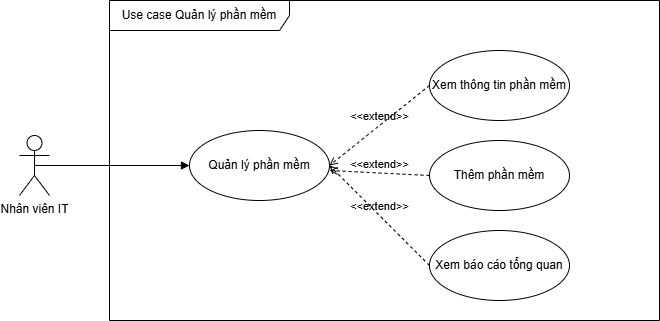
\includegraphics[width=\linewidth]{Images/C5/UseCaseDiagrams/Use-case-Quan-ly-phan-mem.drawio.png}
%     \vspace{5pt}
%     \caption{Use case Quản lý phần mềm}
% \end{figure}
% \begin{table}[H]
%         \centering
%         \caption{Đặc tả Use case Quản lý phần mềm}
%         \begin{tabular}{|p{4cm}|p{10cm}|}
%             \hline
%             Tên use-case & Quản lý phần mềm\\
%             \hline
%             Đối tượng & Nhân viên IT \\
%             \hline
%             Mô tả & Nhân viên IT thực hiện quản lý phần mềm \\
%             \hline
%             Diều kiện kích hoạt & Nhân viên IT bấm nút "Phần mềm" trên giao diện chính của hệ thống \\
%             \hline
%             Tiền điều kiện & Nhân viên IT đã đăng nhập vào hệ thống, có quyền truy cập vào tính năng Quản lý phần mềm. \\
%             \hline
%             Hậu điều kiện & Nhân viên IT thực hiện quản lý phần mềm thành công. \\
%             \hline
%             Luồng tương tác chính & 
%             \begin{enumerate}
%                 \item Nhân viên IT chọn "Phần mềm" ở giao diện chính của hệ thống.
%                 \item Hệ thống hiển thị danh sách các phần mềm.
%                 \item Nhân viên IT chọn phần mềm cần xem chi tiết.
%                 \item Hệ thống hiển thị thông tin chi tiết của phần mềm.
%             \end{enumerate}
%             \\
%             \hline
%             Luồng tương tác thay thế&
            
%             Tại bước 3:
            
%             3.1. Nhân viên IT chọn "Thêm phần mềm" để thêm phần mềm mới.
            
%             3.2. Hệ thống hiển thị giao diện thêm phần mềm.
            
%             3.3. Nhân viên IT nhập thông tin cho phần mềm cần thêm và bấm "Lưu".

%             3.4. Hệ thống kiểm tra và ghi nhận thông tin phần mềm.
%             \newline

%             Tại bước 2:
            
%             2.1. Nhân viên IT chọn "Báo cáo tổng quan".
            
%             2.2. Hệ thống hiển thị báo cáo tổng quan về phần mềm.
%             \\
%             \hline
%             Luồng tương tác ngoại lệ &
            
%             Tại bước 2: Hệ thống lỗi trong việc hiển thị danh sách phần mềm, hệ thống báo lỗi.

%             Tại bước 4: Hệ thống lỗi trong việc hiển thị thông tin phần mềm, hệ thống báo lỗi.

%             Tại bước 2.2: Hệ thống lỗi trong việc hiển thị báo cáo thổng quan về phần mềm, hệ thống báo lỗi.

%             Tại bước 3.4: Hệ thống lỗi trong việc kiểm tra và ghi nhận thông tin phần mềm, hệ thống báo lỗi.
%             \\
%             \hline
%         \end{tabular}
        
%         \label{tab:my_label}
% \end{table}

% \item{ Use case Quản lý giấy phép phần mềm}
% \begin{figure}[H]
%     \centering
%     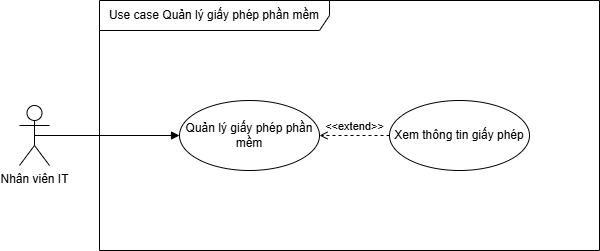
\includegraphics[width=\linewidth]{Images/C5/UseCaseDiagrams/Use-case-Quan-ly-giay-phep-phan-mem.drawio.png}
%     \vspace{5pt}
%     \caption{Use case Quản lý giấy phép phần mềm}
% \end{figure}
% \begin{table}[H]
%         \centering
%         \caption{Đặc tả Use case Quản lý giấy phép phần mềm}
%         \begin{tabular}{|p{4cm}|p{10cm}|}
%             \hline
%             Tên use-case & Quản lý giấy phép phần mềm\\
%             \hline
%             Đối tượng & Nhân viên IT\\
%             \hline
%             Mô tả & Nhân viên IT thực hiện quản lý giấy phép phần mềm. \\
%             \hline
%             Điều kiện kích hoạt & Nhân viên IT bấm vào nút "Giấy phép phần mềm" trên giao diện chính của hệ thống.\\
%             \hline
%             Tiền điều kiện &  Nhân viên IT đã đăng nhập vào hệ thống, có quyền truy cập vào tính năng Quản lý giấy phép phần mềm.\\
%             \hline
%             Hậu điều kiện & Nhân viên IT thực hiện quản lý giấy phép phần mềm thành công \\
%             \hline
%             Luồng tương tác chính & 
%             \begin{enumerate}
%                 \item Nhân viên IT chọn "Giấy phép phần mềm" trên giao diện chính của hệ thống.
%                 \item Hệ thống hiển thị danh sách giấy phép phần mềm.
%                 \item Nhân viên IT chọn giấy phép phần mềm cần xem.
%                 \item Hệ thống hiển thị chi tiết giấy phép phần mềm.
%             \end{enumerate}
%             \\
%             \hline
%             Luồng tương tác thay thế& Không có \\
%             \hline
%             Luồng tương tác ngoại lệ &
%             Tại bước 2: Hệ thống lỗi trong việc hiển thị danh sách giấy phép phần mềm, hệ thống báo lỗi.

%             Tại bước 4: Hệ thống lỗi trong việc hiển thị chi tiết giấy phép phần mềm, hệ thống báo lỗi.
%             \\
%             \hline
%         \end{tabular}
        
%         \label{tab:my_label}
% \end{table}

% \item{ Quản lý cảnh báo}
% \begin{figure}[H]
%     \centering
%     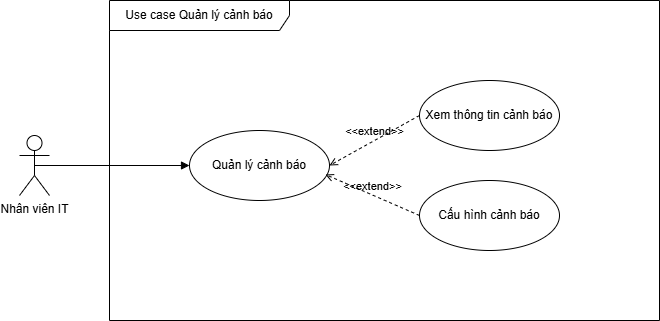
\includegraphics[width=\linewidth]{Images/C5/UseCaseDiagrams/Use-case-Quan-ly-canh-bao.drawio.png}
%     \vspace{5pt}
%     \caption{Use case Quản lý cảnh báo}
% \end{figure}
% \begin{table}[H]
%         \centering
%         \caption{Đặc tả Use case Xem thông tin cảnh báo}
%         \begin{tabular}{|p{4cm}|p{10cm}|}
%             \hline
%             Tên use-case & Xem thông tin cảnh báo\\
%             \hline
%             Đối tượng & Nhân viên IT \\
%             \hline
%             Mô tả & Nhân viên IT thực hiện xem thông tin cảnh báo. \\
%             \hline
%             Diều kiện kích hoạt & Nhân viên IT bấm nút "Cảnh báo" trên giao diện chính của hệ thống \\
%             \hline
%             Tiền điều kiện & Nhân viên IT đã đăng nhập vào hệ thống, có quyền truy cập vào tính năng Quản lý cảnh báo. \\
%             \hline
%             Hậu điều kiện & Nhân viên IT thực hiện xem thông tin cảnh báo thành công. \\
%             \hline
%             Luồng tương tác chính &
%             \begin{enumerate}
%                 \item Nhân viên IT chọn "Cảnh báo" trên giao diện chính của hệ thống.
%                 \item Hệ thống hiển thị danh sách các cảnh báo.
%                 \item Nhân viên IT chọn cảnh báo cần xem chi tiết.
%                 \item Hệ thống hiển chị thông tin chi tiết của cảnh báo.
%             \end{enumerate}\\
%             \hline
%             Luồng tương tác thay thế& Không có \\
%             \hline
%             Luồng tương tác ngoại lệ & 
            
%             Tại bước 2: Hệ thống lỗi trong việc hiển thị danh sách cảnh báo, hệ thống báo lỗi.

%             Tại bước 4: Hệ thống lỗi trong việc hiển thị thông tin cảnh báo, hệ thống báo lỗi.
%             \\
%             \hline
%         \end{tabular}
        
%         \label{tab:my_label}
% \end{table}

% \begin{table}[H]
%         \centering
%         \caption{Đặc tả Use case Cấu hình cảnh báo}
%         \begin{tabular}{|p{4cm}|p{10cm}|}
%             \hline
%             Tên use-case & Cấu hình cảnh báo\\
%             \hline
%             Đối tượng & Nhân viên IT \\
%             \hline
%             Mô tả & b Nhân viên IT thực hiện cấu hình cảnh báo. \\
%             \hline
%             Diều kiện kích hoạt & Nhân viên IT bấm nút "Cấu hình cảnh báo" trên giao diện chính của hệ thống \\
%             \hline
%             Tiền điều kiện & Nhân viên IT đã đăng nhập vào hệ thống, có quyền truy cập vào tính năng Cấu hình cảnh báo. \\
%             \hline
%             Hậu điều kiện & Nhân viên IT thực hiện cấu hình cảnh báo thành công. \\
%             \hline
%             Luồng tương tác chính &
%             \begin{enumerate}
%                 \item Nhân viên IT chọn "Cấu hình cảnh báo" trên giao diện chính của hệ thống (phần Cấu hình).
%                 \item Hệ thống hiển thị giao diện cấu hình cảnh báo.
%                 \item Nhân viên IT thực hiện cấu hình cảnh báo.
%                 \item Hệ thống kiểm tra và lưu cấu hình cảnh báo.
%             \end{enumerate}\\
%             \hline
%             Luồng tương tác thay thế& Không có \\
%             \hline
%             Luồng tương tác ngoại lệ & 
            
%             Tại bước 4: Hệ thống lỗi trong việc kiểm tra và lưu cấu hình cảnh báo, hệ thống báo lỗi.
%             \\
%             \hline
%         \end{tabular}
        
%         \label{tab:my_label}
% \end{table}

% \item{ Quản lý sự cố và bảo trì}
% \begin{figure}[H]
%     \centering
%     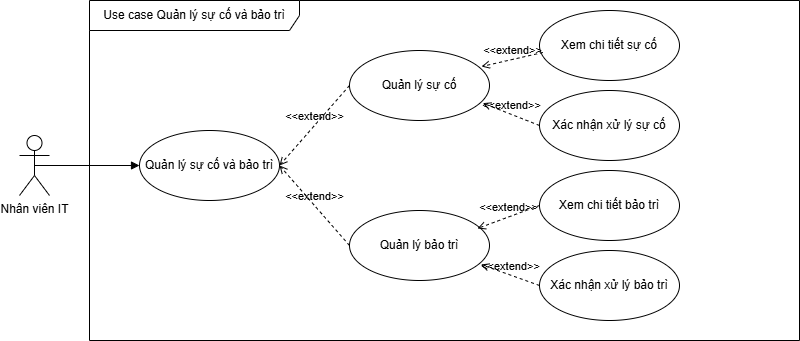
\includegraphics[width=\linewidth]{Images/C5/UseCaseDiagrams/Use-case-Quan-ly-su-co-va-bao-tri.drawio.png}
%     \vspace{5pt}
%     \caption{Use case Quản lý sự cố và bảo trì}
% \end{figure}
% \begin{table}[H]
%         \centering
%         \caption{Đặc tả Use case Quản lý sự cố}
%         \begin{tabular}{|p{4cm}|p{10cm}|}
%             \hline
%             Tên use-case & Quản lý sự cố\\
%             \hline
%             Đối tượng & Nhân viên IT \\
%             \hline
%             Mô tả & b Nhân viên IT thực hiện quản lý sự cố. \\
%             \hline
%             Diều kiện kích hoạt & Nhân viên IT bấm nút "Quản lý sự cố và bảo trì" trên giao diện chính của hệ thống \\
%             \hline
%             Tiền điều kiện & Nhân viên IT đã đăng nhập vào hệ thống, có quyền truy cập vào tính năng Quản lý sự cố. \\
%             \hline
%             Hậu điều kiện & Nhân viên IT thực hiện quản lý sự cố thành công. \\
%             \hline
%             Luồng tương tác chính &
%             \begin{enumerate}
%                 \item Nhân viên IT chọn "Quản lý sự cố và bảo trì" trên giao diện chính của hệ thống và chọn "Danh sách sự cố"
%                 \item Hệ thống hiển thị danh sách sự cố.
%                 \item Nhân viên IT chọn sự cố cần xem chi tiết.
%                 \item Hệ thống hiển thị chi tiết sự cố.
%                 \item Nhân viên IT chọn "Xác nhận đã xử lý" để xác nhận sự cố đã được xử lý.
%                 \item Hệ thống ghi nhận và cập nhật lại trạng thái xử lý.
%             \end{enumerate}\\
%             \hline
%             Luồng tương tác thay thế& Không có \\
%             \hline
%             Luồng tương tác ngoại lệ & 

%             Tại bước 2: Hệ thống lỗi trong việc hiển thị danh sách sự cố, hệ thống báo lỗi.

%             Tại bước 4: Hệ thống lỗi trong việc hiển thị chi tiết sự cố, hệ thống báo lỗi.
            
%             Tại bước 6: Hệ thống lỗi trong việc kiểm tra và ghi nhận cập nhật xử lý sự cố, hệ thống báo lỗi.
%             \\
%             \hline
%         \end{tabular}
        
%         \label{tab:my_label}
% \end{table}

% \begin{table}[H]
%         \centering
%         \caption{Đặc tả Use case Quản lý sự cố}
%         \begin{tabular}{|p{4cm}|p{10cm}|}
%             \hline
%             Tên use-case & Quản lý bảo trì\\
%             \hline
%             Đối tượng & Nhân viên IT \\
%             \hline
%             Mô tả & b Nhân viên IT thực hiện quản lý bảo trì. \\
%             \hline
%             Diều kiện kích hoạt & Nhân viên IT bấm nút "Quản lý sự cố và bảo trì" trên giao diện chính của hệ thống \\
%             \hline
%             Tiền điều kiện & Nhân viên IT đã đăng nhập vào hệ thống, có quyền truy cập vào tính năng Quản lý bảo trì. \\
%             \hline
%             Hậu điều kiện & Nhân viên IT thực hiện quản lý bảo trì thành công. \\
%             \hline
%             Luồng tương tác chính &
%             \begin{enumerate}
%                 \item Nhân viên IT chọn "Quản lý sự cố và bảo trì" trên giao diện chính của hệ thống và chọn "Danh sách yêu cầu bảo trì"
%                 \item Hệ thống hiển thị danh sách yêu cầu bảo trì.
%                 \item Nhân viên IT chọn yêu cầu bảo trì cần xem chi tiết.
%                 \item Hệ thống hiển thị chi tiết yêu cầu bảo trì.
%                 \item Nhân viên IT chọn "Xác nhận hoàn tất" để xác nhận yêu cầu bảo trì đã được xử lý.
%                 \item Hệ thống ghi nhận và cập nhật lại trạng thái xử lý yêu cầu bảo trì.
%             \end{enumerate}\\
%             \hline
%             Luồng tương tác thay thế& Không có \\
%             \hline
%             Luồng tương tác ngoại lệ & 

%             Tại bước 2: Hệ thống lỗi trong việc hiển thị danh sách yêu cầu bảo trì, hệ thống báo lỗi.

%             Tại bước 4: Hệ thống lỗi trong việc hiển thị chi tiết yêu cầu bảo trì, hệ thống báo lỗi.
            
%             Tại bước 6: Hệ thống lỗi trong việc kiểm tra và ghi nhận cập nhật xử lý yêu cầu bảo trì, hệ thống báo lỗi.
%             \\
%             \hline
%         \end{tabular}
        
%         \label{tab:my_label}
% \end{table}

% \item{ Use case Quản lý yêu cầu nâng cấp}
% \begin{figure}[H]
%     \centering
%     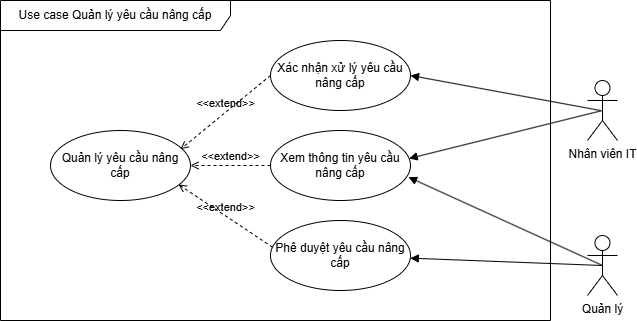
\includegraphics[width=\linewidth]{Images/C5/UseCaseDiagrams/Use-case-Quan-ly-yeu-cau-nang-cap.drawio.png}
%     \vspace{5pt}
%     \caption{Use case Quản lý yêu cầu nâng cấp}
% \end{figure}
% \begin{table}[H]
%         \centering
%         \caption{Đặc tả Use case Xác nhận xử lý yêu cầu nâng cấp}
%         \begin{tabular}{|p{4cm}|p{10cm}|}
%             \hline
%             Tên use-case & Xác nhận xử lý yêu cầu nâng cấp\\
%             \hline
%             Đối tượng & Nhân viên IT \\
%             \hline
%             Mô tả & Nhân viên IT thực hiện xác nhận đã xử lý yêu cầu nâng cấp \\
%             \hline
%             Điều kiện kích hoạt & Nhân viên IT bấm vào nút "Xác nhận xử lý" trên giao diện thông tin chi tiết yêu cầu nâng cấp\\
%             \hline
%             Tiền điều kiện &  Nhân viên IT đã đăng nhập vào hệ thống, có quyền truy cập vào tính năng Quản lý yêu cầu nâng cấp.\\
%             \hline
%             Hậu điều kiện & Nhân viên IT thực hiện xác nhận xử lý yêu cầu nâng cấp thành công \\
%             \hline
%             Luồng tương tác chính & 
%             \begin{enumerate}
%                 \item Nhân viên IT chọn "Yêu cầu nâng cấp" trên giao diện chính của hệ thống.
%                 \item Hệ thống hiển thị danh sách yêu cầu nâng cấp.
%                 \item Nhân viên IT chọn yêu cầu nâng cấp cần xem.
%                 \item Hệ thống hiển thị chi tiết yêu cầu nâng cấp.
%                 \item Nhân viên IT chọn ""Xác nhận xử lý" trên giao diện thông tin chi tiết yêu cầu nâng cấp.
%                 \item Hệ thống kiểm tra và ghi nhận thông tin xác nhận xử lý.
%             \end{enumerate}
%             \\
%             \hline
%             Luồng tương tác thay thế& Không có \\
%             \hline
%             Luồng tương tác ngoại lệ &
%             Tại bước 2: Hệ thống lỗi trong việc hiển thị danh sách yêu cầu nâng cấp, hệ thống báo lỗi.

%             Tại bước 4: Hệ thống lỗi trong việc hiển thị chi tiết yêu cầu nâng cấp, hệ thống báo lỗi.
            
%             Tại bước 6: Hệ thống lỗi trong việc kiểm tra và ghi nhận cập nhật xử lý yêu cầu nâng cấp, hệ thống báo lỗi.
%             \\
%             \hline
%         \end{tabular}
        
%         \label{tab:my_label}
% \end{table}

% \begin{table}[H]
%         \centering
%         \caption{Đặc tả Use case Xem thông tin yêu cầu nâng cấp}
%         \begin{tabular}{|p{4cm}|p{10cm}|}
%             \hline
%             Tên use-case & Xem thông tin yêu cầu nâng cấp\\
%             \hline
%             Đối tượng & Nhân viên IT, Quản lý \\
%             \hline
%             Mô tả & Nhân viên IT, Quản lý thực hiện xem thông tin yêu cầu nâng cấp \\
%             \hline
%             Điều kiện kích hoạt & Nhân viên IT, Quản lý bấm vào nút "Yêu cầu nâng cấp" trên giao diện chính của hệ thống.\\
%             \hline
%             Tiền điều kiện &  Nhân viên IT, Quản lý đã đăng nhập vào hệ thống, có quyền truy cập vào tính năng Quản lý yêu cầu nâng cấp.\\
%             \hline
%             Hậu điều kiện & Nhân viên IT, Quản lý thực hiện xem thông tin yêu cầu nâng cấp thành công \\
%             \hline
%             Luồng tương tác chính & 
%             \begin{enumerate}
%                 \item Nhân viên IT, Quản lý chọn "Yêu cầu nâng cấp" trên giao diện chính của hệ thống.
%                 \item Hệ thống hiển thị danh sách yêu cầu nâng cấp.
%                 \item Nhân viên IT, Quản lý chọn yêu cầu nâng cấp cần xem.
%                 \item Hệ thống hiển thị chi tiết yêu cầu nâng cấp.
%             \end{enumerate}
%             \\
%             \hline
%             Luồng tương tác thay thế& Không có \\
%             \hline
%             Luồng tương tác ngoại lệ &
%             Tại bước 2: Hệ thống lỗi trong việc hiển thị danh sách yêu cầu nâng cấp, hệ thống báo lỗi.

%             Tại bước 4: Hệ thống lỗi trong việc hiển thị chi tiết yêu cầu nâng cấp, hệ thống báo lỗi.
%             \\
%             \hline
%         \end{tabular}
        
%         \label{tab:my_label}
% \end{table}

% \begin{table}[H]
%         \centering
%         \caption{Đặc tả Use case Phê duyệt yêu cầu nâng cấp}
%         \begin{tabular}{|p{4cm}|p{10cm}|}
%             \hline
%             Tên use-case & Phê duyệt yêu cầu nâng cấp\\
%             \hline
%             Đối tượng & Quản lý \\
%             \hline
%             Mô tả & Quản lý thực hiện phê duyệt yêu cầu nâng cấp \\
%             \hline
%             Điều kiện kích hoạt & Quản lý bấm vào nút "Phê duyệt" trên giao diện thông tin chi tiết yêu cầu nâng cấp\\
%             \hline
%             Tiền điều kiện &  Quản lý đã đăng nhập vào hệ thống, có quyền truy cập vào tính năng Quản lý yêu cầu nâng cấp.\\
%             \hline
%             Hậu điều kiện & Quản lý thực hiện phê duyệt yêu cầu nâng cấp thành công \\
%             \hline
%             Luồng tương tác chính & 
%             \begin{enumerate}
%                 \item Quản lý chọn "Yêu cầu nâng cấp" trên giao diện chính của hệ thống.
%                 \item Hệ thống hiển thị danh sách yêu cầu nâng cấp.
%                 \item Quản lý chọn yêu cầu nâng cấp cần xem.
%                 \item Hệ thống hiển thị chi tiết yêu cầu nâng cấp.
%                 \item Quản lý chọn "Phê duyệt" trên giao diện thông tin chi tiết yêu cầu nâng cấp.
%                 \item Hệ thống kiểm tra và ghi nhận thông tin phê duyệt.
%             \end{enumerate}
%             \\
%             \hline
%             Luồng tương tác thay thế& Không có \\
%             \hline
%             Luồng tương tác ngoại lệ &
%             Tại bước 2: Hệ thống lỗi trong việc hiển thị danh sách yêu cầu nâng cấp, hệ thống báo lỗi.

%             Tại bước 4: Hệ thống lỗi trong việc hiển thị chi tiết yêu cầu nâng cấp, hệ thống báo lỗi.
            
%             Tại bước 6: Hệ thống lỗi trong việc kiểm tra và ghi nhận phê duyệt yêu cầu nâng cấp, hệ thống báo lỗi.
%             \\
%             \hline
%         \end{tabular}
        
%         \label{tab:my_label}
% \end{table}

% \item{ Use case Quản lý yêu cầu thanh lý}
% \begin{figure}[H]
%     \centering
%     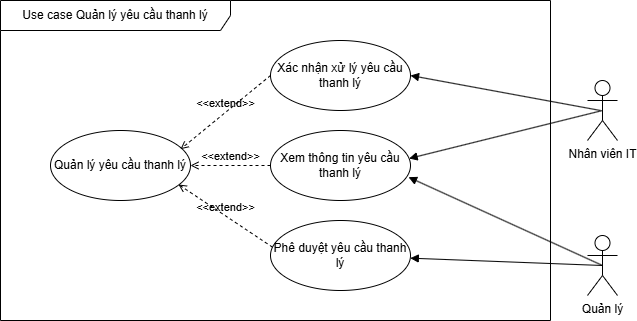
\includegraphics[width=\linewidth]{Images/C5/UseCaseDiagrams/Use-case-Quan-ly-yeu-cau-thanh-ly.drawio.png}
%     \vspace{5pt}
%     \caption{Use case Quản lý yêu cầu thanh lý}
% \end{figure}
% \begin{table}[H]
%         \centering
%         \caption{Đặc tả Use case Xác nhận xử lý yêu cầu thanh lý}
%         \begin{tabular}{|p{4cm}|p{10cm}|}
%             \hline
%             Tên use-case & Xác nhận xử lý yêu cầu thanh lý\\
%             \hline
%             Đối tượng & Nhân viên IT \\
%             \hline
%             Mô tả & Nhân viên IT thực hiện xác nhận đã xử lý yêu cầu thanh lý \\
%             \hline
%             Điều kiện kích hoạt & Nhân viên IT bấm vào nút "Xác nhận xử lý" trên giao diện thông tin chi tiết yêu cầu thanh lý\\
%             \hline
%             Tiền điều kiện &  Nhân viên IT đã đăng nhập vào hệ thống, có quyền truy cập vào tính năng Quản lý yêu cầu thanh lý.\\
%             \hline
%             Hậu điều kiện & Nhân viên IT thực hiện xác nhận xử lý yêu cầu thanh lý thành công \\
%             \hline
%             Luồng tương tác chính & 
%             \begin{enumerate}
%                 \item Nhân viên IT chọn "Yêu cầu thanh lý" trên giao diện chính của hệ thống.
%                 \item Hệ thống hiển thị danh sách yêu cầu thanh lý.
%                 \item Nhân viên IT chọn yêu cầu thanh lý cần xem.
%                 \item Hệ thống hiển thị chi tiết yêu cầu thanh lý.
%                 \item Nhân viên IT chọn ""Xác nhận xử lý" trên giao diện thông tin chi tiết yêu cầu thanh lý.
%                 \item Hệ thống kiểm tra và ghi nhận thông tin xác nhận xử lý.
%             \end{enumerate}
%             \\
%             \hline
%             Luồng tương tác thay thế& Không có \\
%             \hline
%             Luồng tương tác ngoại lệ &
%             Tại bước 2: Hệ thống lỗi trong việc hiển thị danh sách yêu cầu thanh lý, hệ thống báo lỗi.

%             Tại bước 4: Hệ thống lỗi trong việc hiển thị chi tiết yêu cầu thanh lý, hệ thống báo lỗi.
            
%             Tại bước 6: Hệ thống lỗi trong việc kiểm tra và ghi nhận cập nhật xử lý yêu cầu thanh lý, hệ thống báo lỗi.
%             \\
%             \hline
%         \end{tabular}
        
%         \label{tab:my_label}
% \end{table}

% \begin{table}[H]
%         \centering
%         \caption{Đặc tả Use case Xem thông tin yêu cầu thanh lý}
%         \begin{tabular}{|p{4cm}|p{10cm}|}
%             \hline
%             Tên use-case & Xem thông tin yêu cầu thanh lý\\
%             \hline
%             Đối tượng & Nhân viên IT, Quản lý \\
%             \hline
%             Mô tả & Nhân viên IT, Quản lý thực hiện xem thông tin yêu cầu thanh lý \\
%             \hline
%             Điều kiện kích hoạt & Nhân viên IT, Quản lý bấm vào nút "Yêu cầu thanh lý" trên giao diện chính của hệ thống.\\
%             \hline
%             Tiền điều kiện &  Nhân viên IT, Quản lý đã đăng nhập vào hệ thống, có quyền truy cập vào tính năng Quản lý yêu cầu thanh lý.\\
%             \hline
%             Hậu điều kiện & Nhân viên IT, Quản lý thực hiện xem thông tin yêu cầu thanh lý thành công \\
%             \hline
%             Luồng tương tác chính & 
%             \begin{enumerate}
%                 \item Nhân viên IT, Quản lý chọn "Yêu cầu thanh lý" trên giao diện chính của hệ thống.
%                 \item Hệ thống hiển thị danh sách yêu cầu thanh lý.
%                 \item Nhân viên IT, Quản lý chọn yêu cầu thanh lý cần xem.
%                 \item Hệ thống hiển thị chi tiết yêu cầu thanh lý.
%             \end{enumerate}
%             \\
%             \hline
%             Luồng tương tác thay thế& Không có \\
%             \hline
%             Luồng tương tác ngoại lệ &
%             Tại bước 2: Hệ thống lỗi trong việc hiển thị danh sách yêu cầu thanh lý, hệ thống báo lỗi.

%             Tại bước 4: Hệ thống lỗi trong việc hiển thị chi tiết yêu cầu thanh lý, hệ thống báo lỗi.
%             \\
%             \hline
%         \end{tabular}
        
%         \label{tab:my_label}
% \end{table}

% \begin{table}[H]
%         \centering
%         \caption{Đặc tả Use case Phê duyệt yêu cầu thanh lý}
%         \begin{tabular}{|p{4cm}|p{10cm}|}
%             \hline
%             Tên use-case & Phê duyệt yêu cầu thanh lý\\
%             \hline
%             Đối tượng & Quản lý \\
%             \hline
%             Mô tả & Quản lý thực hiện phê duyệt yêu cầu thanh lý \\
%             \hline
%             Điều kiện kích hoạt & Quản lý bấm vào nút "Phê duyệt" trên giao diện thông tin chi tiết yêu cầu thanh lý\\
%             \hline
%             Tiền điều kiện &  Quản lý đã đăng nhập vào hệ thống, có quyền truy cập vào tính năng Quản lý yêu cầu thanh lý.\\
%             \hline
%             Hậu điều kiện & Quản lý thực hiện phê duyệt yêu cầu thanh lý thành công \\
%             \hline
%             Luồng tương tác chính & 
%             \begin{enumerate}
%                 \item Quản lý chọn "Yêu cầu thanh lý" trên giao diện chính của hệ thống.
%                 \item Hệ thống hiển thị danh sách yêu cầu thanh lý.
%                 \item Quản lý chọn yêu cầu thanh lý cần xem.
%                 \item Hệ thống hiển thị chi tiết yêu cầu thanh lý.
%                 \item Quản lý chọn "Phê duyệt" trên giao diện thông tin chi tiết yêu cầu thanh lý.
%                 \item Hệ thống kiểm tra và ghi nhận thông tin phê duyệt.
%             \end{enumerate}
%             \\
%             \hline
%             Luồng tương tác thay thế& Không có \\
%             \hline
%             Luồng tương tác ngoại lệ &
%             Tại bước 2: Hệ thống lỗi trong việc hiển thị danh sách yêu cầu thanh lý, hệ thống báo lỗi.

%             Tại bước 4: Hệ thống lỗi trong việc hiển thị chi tiết yêu cầu thanh lý, hệ thống báo lỗi.
            
%             Tại bước 6: Hệ thống lỗi trong việc kiểm tra và ghi nhận phê duyệt yêu cầu thanh lý, hệ thống báo lỗi.
%             \\
%             \hline
%         \end{tabular}
        
%         \label{tab:my_label}
% \end{table}

% \item{ Use case Quản lý đơn đặt hàng}
% \begin{figure}[H]
%     \centering
%     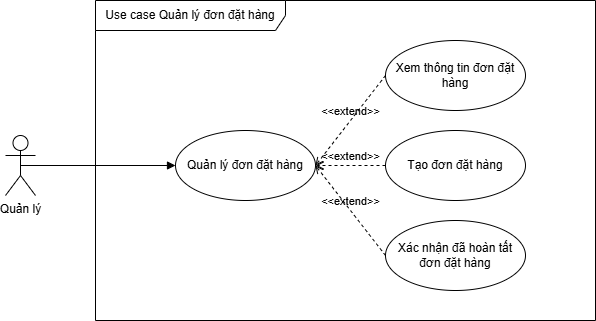
\includegraphics[width=\linewidth]{Images/C5/UseCaseDiagrams/Use-case-Quan-ly-don-dat-hang.drawio.png}
%     \vspace{5pt}
%     \caption{Use case Quản lý đơn đặt hàng}
% \end{figure}

% \begin{table}[H]
%         \centering
%         \caption{Đặc tả Use case Quản lý đơn đặt hàng}
%         \begin{tabular}{|p{4cm}|p{10cm}|}
%             \hline
%             Tên use-case & Quản lý đơn đặt hàng\\
%             \hline
%             Đối tượng & Quản lý \\
%             \hline
%             Mô tả & Quản lý có thể thực hiện quản lý đơn đặt hàng \\
%             \hline
%             Diều kiện kích hoạt & Quản lý chọn "Đơn đặt hàng" trên giao diện chính của hệ thống \\
%             \hline
%             Tiền điều kiện & Quản lý đã đăng nhập vào hệ thống, có quyền truy cập vào tính năng Quản lý đơn đặt hàng \\
%             \hline
%             Hậu điều kiện & Quản lý có thể thực hiện quản lý đơn đặt hàng thành công \\
%             \hline
%             Luồng tương tác chính &
%             \begin{enumerate}
%                 \item Quản lý chọn vào mục "Đơn đặt hàng".
%                 \item Hệ thống hiển thị danh sách đơn đặt hàng.
%                 \item Quản lý chọn đơn đặt hàng cần xem thông tin.
%                 \item Hệ thống hiện thị thông tin về đơn đặt hàng.
%                 \item Quản lý chọn "Xác nhận đã hoàn tất" để xác nhận đơn hàng đã hoàn tất.
%                 \item Hệ thống kiểm tra và ghi nhận hoàn tất đơn hàng.
%             \end{enumerate}\\
%             \hline
%             Luồng tương tác thay thế&  
            
%             Tại bước 2: 
                
%             2.1 Nếu muốn thêm đơn đặt hàng mới, chọn "Thêm đơn đặt hàng"
            
%             2.2. Quản lý nhập thông tin cho đơn đặt hàng và bấm "Đặt hàng"
            
%             2.3. Hệ thống kiểm tra và ghi nhận đơn đặt hàng.
                  
%             \\
%             \hline
%             Luồng tương tác ngoại lệ &

%             Tại bước 2: Hệ thống lỗi trong việc hiển thị danh sách đơn đặt hàng, hệ thống báo lỗi.

%             Tại bước 4: Hệ thống lỗi trong việc hiển thị chi tiết đơn đặt hàng, hệ thống báo lỗi.
            
%             Tại bước 6: Hệ thống lỗi trong việc kiểm tra và ghi nhận cập nhật hoàn tất đơn đặt hàng, hệ thống báo lỗi.
%             \\
%             \hline
%         \end{tabular}
        
%         \label{tab:my_label}
% \end{table}

% % \item{ Use case Quản lý tài chính}
% % \begin{figure}[H]
% %     \centering
% %     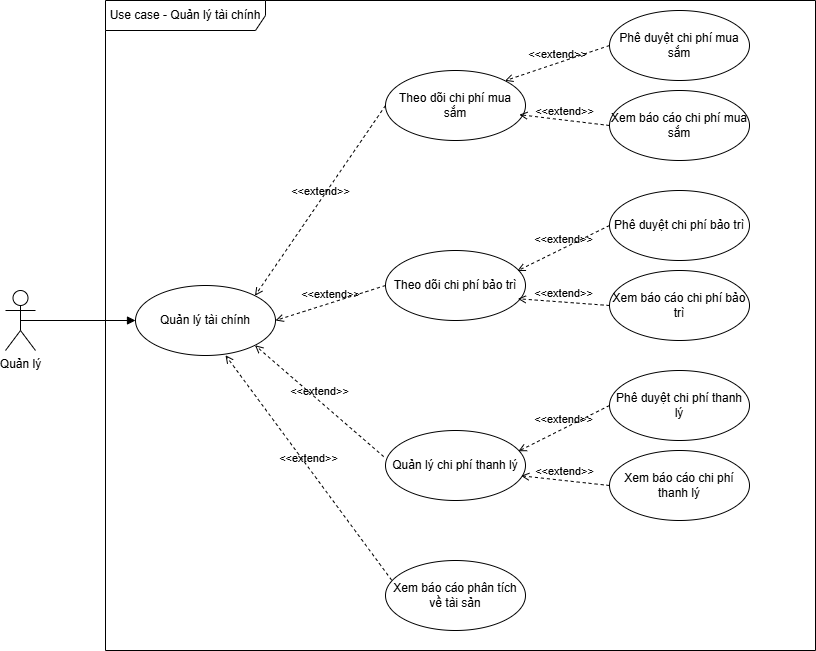
\includegraphics[width=\linewidth]{Images/C5/UseCaseDiagrams/Use-case-Quan-ly-tai-chinh.drawio.png}
% %     \vspace{5pt}
% %     \caption{Use case Quản lý tài chính}
% % \end{figure}
% % \begin{table}[H]
% %         \centering
% %         \begin{tabular}{|p{4cm}|p{10cm}|}
% %             \hline
% %             Tên use-case & Theo dõi chi phí mua sắm\\
% %             \hline
% %             Đối tượng & Quản lý \\
% %             \hline
% %             Mô tả & Quản lý thực hiện theo dõi chi phí mua sắm. \\
% %             \hline
% %             Diều kiện kích hoạt & Quản lý chọn vào "Chi phí mua sắm" trên giao diện quản lý tài chính \\
% %             \hline
% %             Tiền điều kiện & Quản lý đã đăng nhập vào hệ thống, có quyền truy cập vào tính năng Quản lý tài chính. \\
% %             \hline
% %             Hậu điều kiện & Quản lý thực hiện theo dõi chi phí mua sắm thành công. \\
% %             \hline
% %             Luồng tương tác chính &
% %             \begin{enumerate}
% %                 \item Quản lý chọn vào "Tài chính" trên giao diện chính của hệ thống.
% %                 \item Hệ thống hiển thị giao diện quản lý tài chính.
% %                 \item Quản lý chọn vào "Chi phí mua sắm".
% %                 \item Hệ thống hiển thị danh sách chi phí mua sắm.
% %                 \item Quản lý chọn chi phí mua sắm cần quản lý.
% %                 \item Hệ thống hiển thị chi tiết chi phí mua sắm.
% %                 \item Quản lý chọn "Phê duyệt" để phê duyệt chi phí mua sắm.
% %             \end{enumerate}
% %             \\
% %             \hline
% %             Luồng tương tác thay thế& 
% %             Tại bước 3:
% %             3.1. Quản lý chọn "Báo cáo chi phí mua sắm".
% %             3.2. Hệ thống hiển thị báo cáo về chi phí mua sắm.
% %             \\
% %             \hline
% %             Luồng tương tác ngoại lệ &
% %             Tại bước 4: Hệ thống lỗi trong việc hiển thị danh sách chi phí mua sắm, hệ thống báo lỗi.

% %             Tại bước 6: Hệ thống lỗi trong việc hiển thị chi tiết chi phí mua sắm, hệ thống báo lỗi.
            
% %             Tại bước 3.2: Hệ thống lỗi trong việc hiển thị báo cáo chi phí mua sắm, hệ thống báo lỗi.
% %             \\
% %             \hline
% %         \end{tabular}
% %         \caption{Đặc tả Use case Theo dõi chi phí mua sắm}
% %         \label{tab:my_label}
% % \end{table}

% % \begin{table}[H]
% %         \centering
% %         \begin{tabular}{|p{4cm}|p{10cm}|}
% %             \hline
% %             Tên use-case & Theo dõi chi phí bảo trì\\
% %             \hline
% %             Đối tượng & Quản lý \\
% %             \hline
% %             Mô tả & Quản lý thực hiện theo dõi chi phí bảo trì. \\
% %             \hline
% %             Diều kiện kích hoạt & Quản lý chọn vào "Chi phí bảo trì" trên giao diện quản lý tài chính.\\
% %             \hline
% %             Tiền điều kiện & Quản lý đã đăng nhập vào hệ thống, có quyền truy cập vào tính năng Quản lý tài chính. \\
% %             \hline
% %             Hậu điều kiện & Quản lý thực hiện theo dõi chi phí bảo trì thành công. \\
% %             \hline
% %             Luồng tương tác chính &
% %             \begin{enumerate}
% %                 \item Quản lý chọn vào "Tài chính" trên giao diện chính của hệ thống.
% %                 \item Hệ thống hiển thị giao diện quản lý tài chính.
% %                 \item Quản lý chọn vào "Chi phí bảo trì".
% %                 \item Hệ thống hiển thị danh sách chi phí bảo trì.
% %                 \item Quản lý chọn chi phí bảo trì cần quản lý.
% %                 \item Hệ thống hiển thị chi tiết chi phí bảo trì.
% %                 \item Quản lý chọn "Phê duyệt" để phê duyệt chi phí bảo trì.
% %             \end{enumerate}
% %             \\
% %             \hline
% %             Luồng tương tác thay thế& 
% %             Tại bước 3:
% %             3.1. Quản lý chọn "Báo cáo chi phí bảo trì".
% %             3.2. Hệ thống hiển thị báo cáo về chi phí bảo trì.
% %             \\
% %             \hline
% %             Luồng tương tác ngoại lệ &
% %             Tại bước 4: Hệ thống lỗi trong việc hiển thị danh sách chi phí bảo trì, hệ thống báo lỗi.

% %             Tại bước 6: Hệ thống lỗi trong việc hiển thị chi tiết chi phí bảo trì, hệ thống báo lỗi.
            
% %             Tại bước 3.2: Hệ thống lỗi trong việc hiển thị báo cáo chi phí bảo trì, hệ thống báo lỗi.
% %             \\
% %             \hline
% %         \end{tabular}
% %         \caption{Đặc tả Use case Theo dõi chi phí bảo trì}
% %         \label{tab:use_case_maintenance}
% % \end{table}

% % \begin{table}[H]
% %         \centering
% %         \begin{tabular}{|p{4cm}|p{10cm}|}
% %             \hline
% %             Tên use-case & Quản lý chi phí thanh lý\\
% %             \hline
% %             Đối tượng & Quản lý \\
% %             \hline
% %             Mô tả & Quản lý thực hiện theo dõi và quản lý chi phí thanh lý. \\
% %             \hline
% %             Diều kiện kích hoạt & Quản lý chọn vào "Chi phí thanh lý" trên giao diện quản lý tài chính. \\
% %             \hline
% %             Tiền điều kiện & Quản lý đã đăng nhập vào hệ thống, có quyền truy cập vào tính năng Quản lý tài chính. \\
% %             \hline
% %             Hậu điều kiện & Quản lý thực hiện theo dõi và quản lý chi phí thanh lý thành công. \\
% %             \hline
% %             Luồng tương tác chính &
% %             \begin{enumerate}
% %                 \item Quản lý chọn vào "Tài chính" trên giao diện chính của hệ thống.
% %                 \item Hệ thống hiển thị giao diện quản lý tài chính.
% %                 \item Quản lý chọn vào "Chi phí thanh lý".
% %                 \item Hệ thống hiển thị danh sách chi phí thanh lý.
% %                 \item Quản lý chọn chi phí thanh lý cần quản lý.
% %                 \item Hệ thống hiển thị chi tiết chi phí thanh lý.
% %                 \item Quản lý chọn "Phê duyệt" để phê duyệt chi phí thanh lý.
% %             \end{enumerate}
% %             \\
% %             \hline
% %             Luồng tương tác thay thế& 
% %             Tại bước 3:
% %             3.1. Quản lý chọn "Báo cáo chi phí thanh lý".
% %             3.2. Hệ thống hiển thị báo cáo về chi phí thanh lý.
% %             \\
% %             \hline
% %             Luồng tương tác ngoại lệ &
% %             Tại bước 4: Hệ thống lỗi trong việc hiển thị danh sách chi phí thanh lý, hệ thống báo lỗi.

% %             Tại bước 6: Hệ thống lỗi trong việc hiển thị chi tiết chi phí thanh lý, hệ thống báo lỗi.
            
% %             Tại bước 3.2: Hệ thống lỗi trong việc hiển thị báo cáo chi phí thanh lý, hệ thống báo lỗi.
% %             \\
% %             \hline
% %         \end{tabular}
% %         \caption{Đặc tả Use case Quản lý chi phí thanh lý}
% %         \label{tab:use_case_disposal}
% % \end{table}

% % \begin{table}[H]
% %         \centering
% %         \begin{tabular}{|p{4cm}|p{10cm}|}
% %             \hline
% %             Tên use-case & Xem báo cáo và phân tích về tài sản\\
% %             \hline
% %             Đối tượng & Quản lý \\
% %             \hline
% %             Mô tả & Quản lý thực hiện xem báo cáo và phân tích về tài sản. \\
% %             \hline
% %             Diều kiện kích hoạt & Quản lý chọn vào "Báo cáo về tài sản" trên giao diện quản lý tài chính. \\
% %             \hline
% %             Tiền điều kiện & Quản lý đã đăng nhập vào hệ thống, có quyền truy cập vào tính năng Quản lý tài chính. \\
% %             \hline
% %             Hậu điều kiện & Quản lý thực hiện xem báo cáo và phân tích về tài sản thành công. \\
% %             \hline
% %             Luồng tương tác chính &
% %             \begin{enumerate}
% %                 \item Quản lý chọn vào "Tài chính" trên giao diện chính của hệ thống.
% %                 \item Hệ thống hiển thị giao diện quản lý tài chính.
% %                 \item Quản lý chọn vào "Báo cáo về tài sản".
% %                 \item Hệ thống hiển thị báo cáo và phân tích về tài sản.

% %             \end{enumerate}
% %             \\
% %             \hline
% %             Luồng tương tác thay thế& 
% %             Không có
% %             \\
% %             \hline
% %             Luồng tương tác ngoại lệ &
% %             Tại bước 4: Hệ thống lỗi trong việc hiển thị báo cáo và phân tích về tài sản, hệ thống báo lỗi.
% %             \\
% %             \hline
% %         \end{tabular}
% %         \caption{Đặc tả Use case Xem báo cáo và phân tích về tài sản}
% %         \label{tab:use_case_disposal}
% % \end{table}

% \item{ Use case Quản lý cấu hình hệ thống}
% \begin{figure}[H]
%     \centering
%     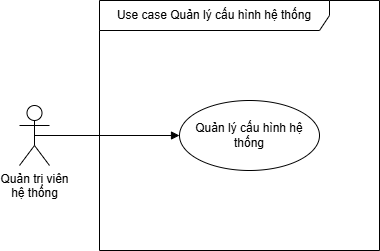
\includegraphics[width=0.7\linewidth]{Images/C5/UseCaseDiagrams/Use-case-Quan-ly-cau-hinh-he-thong.drawio.png}
%     \vspace{15pt}
%     \caption{Use case Quản lý cấu hình hệ thống}
% \end{figure}
% \begin{table}[H]
%         \centering
%         \caption{Đặc tả Use case Quản lý cấu hình hệ thống}
%         \begin{tabular}{|p{4cm}|p{10cm}|}
%             \hline
%             Tên use-case & Quản lý cấu hình hệ thống\\
%             \hline
%             Đối tượng & Quản trị viên hệ thống\\
%             \hline
%             Mô tả & Quản trị viên hệ thống thực hiện quản lý cấu hình hệ thống. \\
%             \hline
%             Điều kiện kích hoạt & Quản trị viên hệ thống chọn vào "Cấu hình chung" trên giao diện chính của hệ thống.\\
%             \hline
%             Tiền điều kiện & Quản trị viên hệ thống đã đăng nhập vào hệ thống, có quyền truy cập vào tính năng Quản lý cấu hình hệ thống. \\
%             \hline
%             Hậu điều kiện & Quản trị viên hệ thống thực hiện quản lý cấu hình hệ thống thành công. \\
%             \hline
%             Luồng tương tác chính & 
%             \begin{enumerate}
%                 \item Quản trị viên hệ thống chọn "Cấu hình chung" trên giao diện chính của hệ thống.
%                 \item Hệ thống hiển thị giao diện cấu hình hệ thống.
%                 \item Quản trị viên hệ thống thực hiện cấu hình hệ thống.
%                 \item Hệ thống kiểm tra và ghi nhận cấu hình.
%             \end{enumerate}
%             \\
%             \hline
%             Luồng tương tác thay thế& Không có \\
%             \hline
%             Luồng tương tác ngoại lệ &
%             Tại bước 4: Hệ thống lỗi trong việc kiểm tra và ghi nhận cấu hình, hệ thống báo lỗi.
%             \\
%             \hline
%         \end{tabular}
        
%         \label{tab:my_label}
% \end{table}

% \end{itemize}

% \subsection{ Giải pháp công nghệ}

% \subsubsection{ Thu thập dữ liệu thời gian thực}
% \begin{enumerate}
%     \item \textbf{Dữ liệu thời gian thực}:
%     \begin{itemize}[label=--]
%         \item \textbf{Dữ liệu thời gian thực (real-time data)}: là dữ liệu được tạo ra và xử lý ngay lập tức, phản ánh trạng thái hiện tại của một hệ thống, sự kiện hoặc hiện tượng. Đặc trưng của loại dữ liệu này là tính tức thời, yêu cầu  phải được xử lý và sử dụng ngay trong thời điểm phát sinh để đảm bảo giá trị và ý nghĩa.\cite{rtd}
%         % \item Tầm quan trọng: 
%         % \begin{itemize}
%         %     \item Ra quyết định nhanh chóng và chính xác
%         %     \item Phản ứng nhanh chóng với sự thay đổi
%         %     \item Cải thiện trải nghiệm người dùng
%         %     \item Tối ưu hóa hiệu quả hoạt động
%         %     \item Nâng cao khả năng cạnh tranh
%         % \end{itemize}
%         \item \textbf{Đặc điểm nổi bật:} 
%         \begin{itemize}[label=\textbullet]
%             \item Tính thức thời: Dữ liệu được tạo ra và xử lý ngay lập tức, thông tin phản ánh trạng thái hiện tại của hệ thống, sự kiện hoặc hiện tượng. Ví dụ: Lượt truy cập website, chỉ số cảm biến từ IoT,...
%             \item Tính liên tục: Dữ liệu được tạo ra liên tục tạo thành một luồng dữ liệu không ngừng, điều này yêu cầu hệ thống phải hoạt động liên tục và ổn định. Ví dụ: nhật ký sự kiện hệ thống
%             \item Tính biến động: dữ liệu có thể thay đổi nhanh chóng và khó dự đoán, điều này yêu cầu hệ thống phải xử lý linh hoạt, thích ứng với sự thay đổi. Ví dụ như: giá cả hàng hóa, giá cổ phiếu biến động trên thị trường chứng khoán.
%             \item Tính ngắn hạn: Giá trị dữ liệu chỉ có ý nghĩa trong thời gian ngắn, dữ liệu cũ có thể bị loại bỏ hoặc lưu trữ với mức độ ưu tiên thấp hơn. Ví dụ như: cảnh báo của hệ thống, định vị, các thông báo. 
%         \end{itemize}
%         \item \textbf{Phân loại dữ liệu thời gian thực}\cite{trtd}:
%         \begin{table}[H]
%         \centering
%         \caption{Loại dữ liệu thời gian thực}
%         \begin{tabular}{|p{2cm}|p{5.5cm}|p{5.5cm}|}
%             \hline
%             \textbf{Đặc điểm} & \textbf{Event Data} & \textbf{Streaming Data} \\
%             \hline
%             Bản chất &
%                 Là dữ liệu gắn nhãn thời gian không đều đặn, được tạo ra khi một sự kiện cụ thể xảy ra. Mỗi sự kiện mang thông tin về sự thay đổi trạng thái của hệ thống
%             &  Là dữ liệu gắn nhãn thời gian đều đặn, được tạo ra dưới dạng một luồng không ngừng, phản ánh trạng thái động của hệ thống. Ví dụ: cách mỗi giây\\
%             \hline
%            Tính chất & Mang tính chất "thời điểm", gắn liền với một mốc thời gian cụ thể &
%            Mang tính chất "thời gian", liên tục thay đổi theo thời gian.\\
%             \hline
%             Cấu trúc & Thường có cấu trúc rõ ràng, chứa thông tin về loại sự kiện, thời gian, đối tượng liên quan,... & Có thể có cấu trúc hoặc không cấu trúc. \\
%             \hline
%             Ví dụ & \begin{itemize}
%                 \item Khách hàng đặt hàng trên Website (sự kiện "đặt hàng")
%                 \item Hệ thống cảnh báo lỗi (sự kiện "lỗi hệ thống")
%             \end{itemize} & \begin{itemize}
%                 \item Dữ liệu cảm biến từ thiết bị IoT
%                 \item Nhật ký sự kiện hệ thống
%                 \item Luồng video từ camera giám sát.
%             \end{itemize}
%             \\
%             \hline
%         \end{tabular}
        
%         \label{tab:my_label}
%     \end{table}
%     \end{itemize}
%        \item \textbf{Apache Kafka trong thu thập dữ liệu thời gian thực}
%         \begin{enumerate}
%             \item \textbf{Các thành phần của Kafka}
%             \begin{figure}[H]
%                 \centering
%                 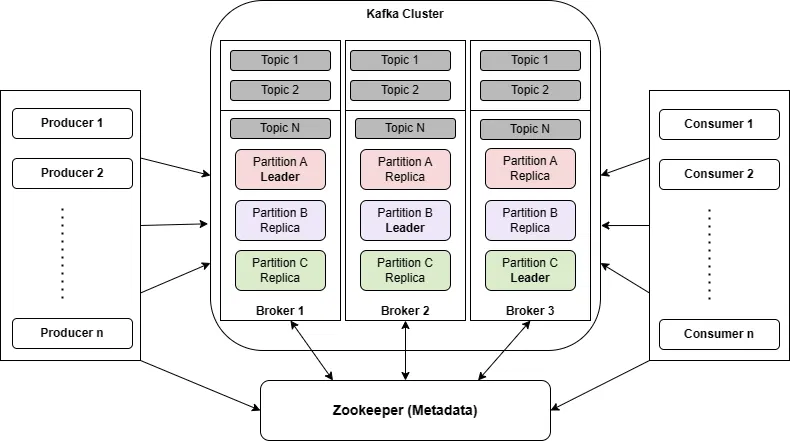
\includegraphics[width=\linewidth]{Images/Kafka/KafkaArchitecture.png}
%                 \vspace{5pt}
%                 \caption{Kiến trúc Kafka\\ Nguồn: 200lab.io, truy cập vào ngày 01/05/2025}
%             \end{figure}
%             \begin{enumerate}
%         \item \textbf{Kafka Events}\\
%         Một Kafka event (sự kiện) còn được gọi là record (bản ghi) hoặc message (thông điệp). Việc sử dụng 3 thuật ngữ event, record và message mang nghĩa tương đương nhau. Hay chỉ đơn giản nó là đơn vị dữ liệu cơ bản trong Kafka, là một mảng byte không có định dạng cụ thể.
    
%         Việc đọc và ghi dữ liệu trong Kafka thực hiện thông qua event. Mỗi event chứa một key (khoá), value (giá trị) và metadata (nếu có).
%     \\
%     \{\\
%     key: "ID",\\
%     value: "2433.544",\\
%     timestamp: "Feb. 12, 2024, at 20:06 p.m."\\
%     \}
%         \item \textbf{Kafka Topics}:
%         \begin{itemize}[label=--]
%         \item Các event được tổ chức và lưu trữ lâu dài trong các topics (chủ đề). Có thể coi một topic ví như một thư mục (folder) trong hệ thống tập tin (filesystem), còn mỗi event là một tập tin (file) nằm bên trong thư mục đó.
%         \item Hình dưới cho thấy một topic có 4 partitions, với phần ghi được thêm vào cuối mỗi partition. Kafka cung cấp khả năng dự phòng (redundancy) và khả năng mở rộng (scalability) thông qua các partitions. Mỗi partition có thể được lưu trữ trên một máy chủ khác nhau, điều đó có nghĩa là một topic có thể được mở rộng theo chiều ngang trên nhiều máy chủ để cung cấp hiệu suất vượt xa khả năng của một máy chủ.
%         \end{itemize}
%         \begin{figure}[H]
%             \centering
%             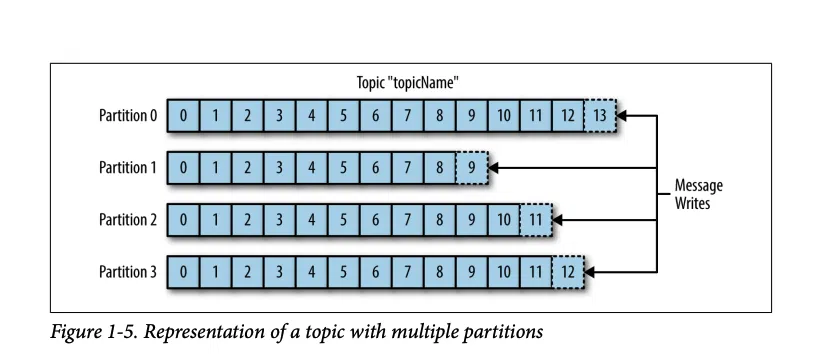
\includegraphics[width=\linewidth]{Images/Kafka/KafkaTopic.png}
%             \vspace{5pt}
%             \caption{Kafka Topic\\ Nguồn: 200lab.io, truy cập vào ngày 01/05/2025}
%         \end{figure}
        
%         \item \textbf{Kafka Brokers và Kafka Clusters}
%         \begin{itemize}[label=--]
%            \item Kafka được chạy dưới dạng một \textbf{Kafka cluster} gồm một hoặc nhiều \textbf{Kafka server} có thể mở rộng trên nhiều data center hoặc cloud. Một Kafka server này tạo thành lớp lưu trữ, được gọi là\textbf{ Kafka broker}.
%             \item \textbf{Brokers} chịu trách nhiệm quản lý bộ lưu trữ, xử lý các yêu cầu đọc và ghi cũng như sao chép dữ liệu trên toàn cluster (cụm).
%             \item Trong mỗi cluster sẽ có một broker sẽ hoạt động như một \textbf{cluster controller} (bộ điều khiển cụm), chịu trách nhiệm chỉ định phân vùng cho brokers và theo dõi lỗi của brokers.
%         \end{itemize}
%         \item \textbf{ Kafka Partitions và Kafka Replication}
%         \begin{itemize}[label=--]
%             \item Các \textbf{topic} được chia thành các \textbf{partitions} (phân vùng), là \textbf{đơn vị cơ bản} của tính song song và phân phối trong Kafka. Mỗi phân vùng được lưu trữ trên \textbf{một broker duy nhất} và nhiều phân vùng cho phép mở rộng quy mô theo chiều ngang và cải thiện hiệu suất.
%              \item Mỗi event trong một partition được gán một \textbf{offset} duy nhất, bắt đầu từ 0 cho event đầu tiên trong partition và tăng dần một cho mỗi event tiếp theo. Offset được sử dụng để xác định vị trí của event trong một partition.
%             \item Kafka đảm bảo độ bền của dữ liệu bằng cách sao chép dữ liệu (replication) trên nhiều brokers. Mỗi partition có thể có một hoặc nhiều \textbf{replica (bản sao)} trên các brokers khác nhau, ngăn ngừa mất dữ liệu trong trường hợp broker lỗi.
%             \begin{figure}[H]
%                 \centering
%                 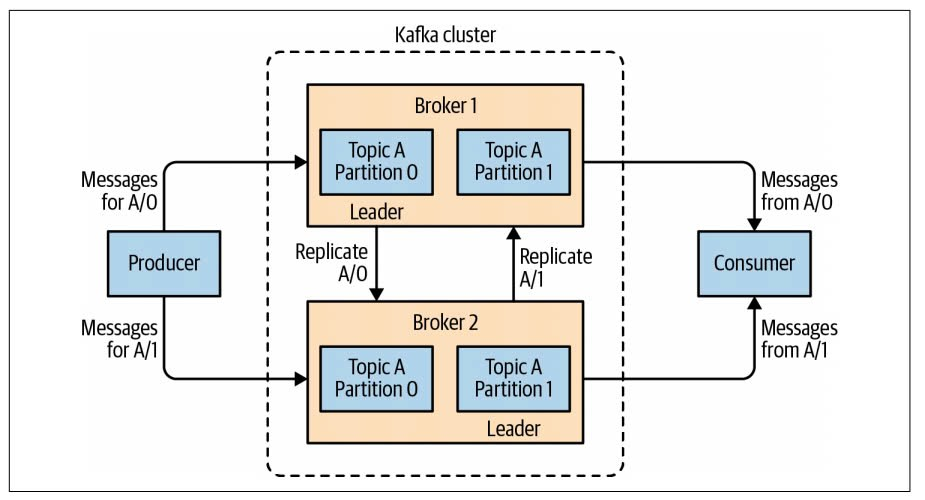
\includegraphics[width=\linewidth]{Images/Kafka/kafkacluster.png}
%                 \vspace{5pt}
%                 \caption{Kafka Cluster\\ Nguồn: 200lab.io, truy cập vào ngày 01/05/2025}
%             \end{figure}
%             \item Mỗi partition có một broker được chỉ định làm \textbf{leader}, nắm quyền sở hữu partition đó, trong khi các \textbf{brokers} còn lại lưu trữ các \textbf{replicas} (bản sao) của phân vùng đó được gọi là \textbf{followers}.
%             Nếu leader broker xảy ra lỗi, một trong những followers có dữ liệu cập nhật sẽ được chọn làm leader mới. Quá trình này được gọi là leader failover (chuyển đổi dự phòng lãnh đạo), nhằm đảm bảo tính khả dụng của dữ liệu.
%         \end{itemize}
%         \item \textbf{Kafka Producers}
%             \begin{itemize}[label=--]
%                 \item \textbf{Kafka Producer} là một client appication (ứng dụng khách), \textbf{publish} (xuất bản) event vào một topic cụ thể trong Kafka và luôn ghi vào \textbf{leader broker}. Theo mặc định, producers không quan tâm tới event được ghi ở partition nào mà sẽ publish đều event trên tất cả partition của một topic. Trong vài trường hợp, một producer sẽ gửi trực tiếp event tới các partition cụ thể.
%                 \item \textbf{Producers} kết nối tới \textbf{Kafka Brokers} thông qua giao thức mạng TCP. Đây là kết nối hai chiều (bi-directional connection).
%             \end{itemize}
%         \begin{figure}[H]
%             \centering
%             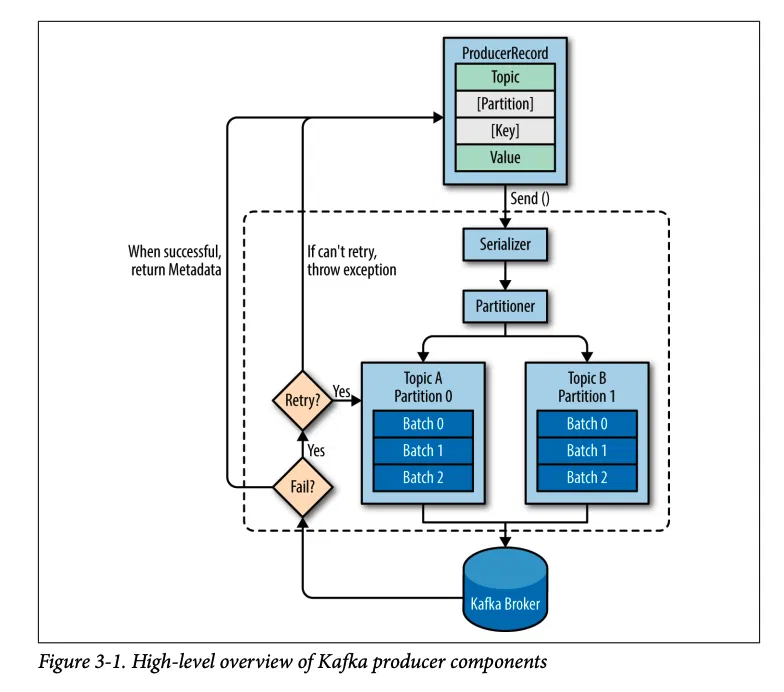
\includegraphics[width=0.7\linewidth]{Images/Kafka/KafkaProducer.png}
%             \vspace{5pt}
%             \caption{Kafka Producer\\ Nguồn: 200lab.io, truy cập vào ngày 01/05/2025}
%         \end{figure}
%         Quá trình gửi event như sau :
%         \begin{itemize}[label=--]
%             \item Tạo produceRecord
%             \item Serializer: Trước khi gửi ProducerRecord qua network, producer sẽ serialize (tuần tự hoá) key và value thành ByteArrays (mảng các bytes).
%             \item Xác định số Partitions: Nếu chúng ta chỉ định sẵn partition thì partitioner sẽ trả về partition được chỉ định, còn không thì partitioner sẽ chọn một partition dựa vào ProducerRecord key.
%             \item  Brokers xử lý events và trả về kết quả cho producers khi biết event cần được gửi tới topic và partition nào, producer sẽ thêm event vào một lô các bản ghi (a batch of records). Từ đó, chúng sẽ được gửi đi cùng topic và partition. Một thread độc lập chịu trách nhiệm gửi các lô bản ghi tới Kafka brokers phù hợp.\\
%             Broker sẽ gửi lại một response khi nhận được events. Nếu event được ghi thành công vào Kafka, broker sẽ gửi lại một object chứa RecordMetadata bao gồm topic, partition và offset của record bên trong partition. Còn nếu không thành công thì broker trả về lỗi. Khi producer nhận được lỗi, event sẽ được gửi lại (retry) vài lần trước khi bỏ cuộc và trả về lỗi.
%         \end{itemize}
%         \item \textbf{Kafka Consumers}: 
%             \begin{itemize}[label=--]
%                 \item \textbf{Kafka consumer} là một client application (ứng dụng khách), subscribe (đăng ký) một hoặc nhiều Kafka topics và đọc các bản ghi theo thứ tự chúng được tạo ra. Consumers đọc dữ liệu theo thời gian thực hoặc theo tốc độ của riêng chúng, cho phép các ứng dụng phản ứng với các sự kiện khi chúng xảy ra.
%                 \item Consumers kết nối tới Kafka Brokers thông qua giao thức mạng TCP. Đây là kết nối hai chiều (bi-directional connection).
%                 \item Consumers hoạt động trong một consumer group, làm việc cùng nhau để xử lý dữ liệu từ các partitions, cung cấp khả năng mở rộng theo chiều ngang và cho phép nhiều phiên bản của cùng một ứng dụng xử lý dữ liệu đồng thời.
%             \end{itemize}
%         \end{enumerate}
%     \end{enumerate}
%     \item \textbf{Công nghệ xử lý dữ liệu thời gian thực}:
%     \begin{enumerate}
%         \item \textbf{Giới thiệu về RabbitMQ}\\
%         \textbf{RabbitMQ} là một message broker (phần mềm trung gian nhắn tin) mã nguồn mở. Nó được thiết kế để hỗ trợ giao tiếp giữa các ứng dụng, hệ thống hoặc dịch vụ bằng cách gửi, nhận và quản lý các message.\\
%         Cách vận hành của RabbitMQ:
%         \begin{itemize}[label=--]
%             \item Producer: Gửi message tới RabbitMQ.
%             \item Exchange: Xử lý và định tuyến message đến các hàng đợi phù hợp dựa trên các rules (routing).
%             \item Queue: Lưu trữ tạm thời các message.
%             \item Consumer: Nhận message từ queue để xử lý.
%         \end{itemize}
%         RabbitMQ cho phép định tuyến linh hoạt thông qua các kiểu exchange: direct, topic, fanout, và headers.\\
%         Một số đặc điểm của RabbitMQ:
%         \begin{itemize}[label=--]
%             \item Mã nguồn mở: RabbitMQ dược viết bằng mã nguồn mở nên các nhà phát triển và kỹ sư trong cộng đồng RabbitMQ có thể đóng góp cải tiến và tiện ích bổ sung, đồng thời tận dụng được sự hỗ trợ tài chính của công ty Pivotal.
%             \item Nhẹ và dễ triển khai:  RabbitMQ dễ cài đặt, cấu hình và phù hợp với các hệ thống nhỏ đến vừa.
%             \item Độ tin cậy: RabbitMQ cho phép các message được chỉ định mức độ ưu tiên khác nhau. Điều này đảm bảo rằng các message có mức độ ưu tiên cao sẽ được xử lý trước các message có mức độ ưu tiên thấp hơn.
%             \item Tính linh hoạt trong kiểm soát cân bằng tin nhắn: RabbitMQ cung cấp các mức QoS khác nhau như "At Most Once" (Tối đa một lần), "At Least Once" (Tối thiểu một lần) và "Exactly Once" (Đúng một lần), cho phép kiểm soát sự cân bằng giữa reliability (độ tin cậy) và performance (hiệu suất).
%             \item Hỗ trợ ngôn ngữ và giao thức linh hoạt: RabbitMQ hỗ trợ chạy trên nhiều hệ điều hành và cả trên môi trường cloud, đồng thời cung cấp nhiều client libraries cho hầu hết các ngôn ngữ lập trình phổ biến. Ngoài ra, RabbitMQ còn hỗ trợ các giao thức nhắn tin khác nhau như STOMP, MQTT, ...
%         \end{itemize}
%         \item \textbf{Giới thiệu về Apache Pulsar}\\
%         \textbf{Apache Pulsar} là một nền tảng messaging phân tán mã nguồn mở, được thiết kế để cung cấp khả năng publish-subscribe (pub-sub) với độ trễ thấp và khả năng mở rộng cao. Pulsar được phát triển bởi Yahoo và hiện là một dự án của Apache Software Foundation, nổi bật nhờ khả năng kết hợp giữa message streaming và message queueing.\\
%         Pulsar sử dụng mô hình topic-based publish-subscribe với kiến trúc 3 thành phần chính:
%         \begin{itemize}[label=--]
%             \item Producer: Gửi các message đến topic.
%             \item Broker: Xử lý và phân phối message tới consumers.
%             \item Consumer: Nhận và xử lý message từ topic.
%         \end{itemize}
%         Một số đặc trưng của Apache Pulsar:
%         \begin{itemize}[label=--]
%             \item Hỗ trợ Message Queue và Pub-Sub: Pulsar cung cấp cả hai cơ chế trong cùng một hệ thống, linh hoạt hơn so với nhiều giải pháp khác.
%             \item Độ trễ thấp và thông lượng cao: Pulsar tối ưu cho các ứng dụng yêu cầu xử lý thời gian thực.
%             \item Hỗ trợ Multi-tenancy: Dễ dàng quản lý nhiều tenant (người dùng hoặc hệ thống độc lập) trên cùng một cụm Pulsar.
%             \item Kiến trúc phân cụm (Clustered Architecture): Pulsar hỗ trợ triển khai cụm để đảm bảo tính sẵn sàng cao (high availability) và khả năng chịu lỗi (fault-tolerance).
%         \end{itemize}
%         \item \textbf{So sánh giữa Kafka với RabbitMQ và Pulsar}\\
%         Các số liệu so sánh được dựa trên các chỉ số mà Confluent cung cấp\cite{compare-kafka}
%         \begin{table}[H]
%             \centering
%             \caption{So sánh giữa các công nghệ xử lý thời gian thực}
%             \begin{tabular}{|p{3cm}|p{3cm}|p{3cm}|p{4cm}|}
%         \hline 
%         \textbf{Khía cạnh} &\textbf{Kafka}  & \textbf{Pulsar} &\textbf{RabbitMQ(AMQP)} \\ 
%         \hline 
%         Thành phần & Kafka + Zookeeper & Pulsar + Zookeeper +
%         BookKeeper +
%         RocksDB & RabbitMQ
%         \\
%         \hline
%         Mô hình tiêu thụ message & Pull & Push & Push 
%         \\
%         \hline 
%         Kiến trúc lưu trữ & Log & Index & Index
%         \\
%         \hline 
%         Thông lượng & 605 MB/s & 305 MB/s & 38 MB/s  
%         \\
%         \hline
%         Độ trễ & 5 ms & 25 ms & 1 ms (*)
%         \\
%         \hline
%         Cộng đồng & Lớn & Chưa phát triển & Tương đối\\ 
%         \hline
%         Khả năng cấu hình & Tương đối phức tạp & Phức tạp & Dễ dàng\\
%         \hline 
%         Lưu trữ lâu dài & Hỗ trợ lưu trữ lâu dài & Hỗ trợ lưu trữ lâu dài  & Không hỗ trợ\\
%         \hline
%         \end{tabular}
          
%             \label{table:comparison}
%         \end{table}
%     (*) Độ trễ của RabbitMQ giảm đáng kể khi thông lượng cao hơn 30 MB/s. \\
%     => Apache Kafka vẫn là lựa chọn khả thi nhất cho thiết kế hệ thống theo mục tiêu đề tài, nhờ khả năng xử lý dữ liệu lớn, lưu trữ lâu dài và thông lượng cao. Tuy Apache Pulsar là lựa chọn tốt nếu hệ thống cần các tính năng cao cấp như quản lý đa cụm linh hoạt hoặc lưu trữ theo tầng. Tuy nhiên, độ phức tạp khi triển khai và hiệu suất chưa thực sự vượt qua Kafka. Đối với RabbitMQ, RabbitMQ chỉ phù hợp nếu cần một hệ thống đơn giản để xử lý message nhỏ và không yêu cầu lưu trữ dữ liệu lâu dài hoặc mở rộng quy mô lớn.
%     \end{enumerate}
%     \item \textbf{Confluent Cloud}:\\
%     Việc triển khai và vận hành \textbf{Apache Kafka} truyền thống yêu cầu doanh nghiệp phải đầu tư nhiều vào hạ tầng, cấu hình, bảo trì và đội ngũ kỹ thuật có chuyên môn cao để đảm bảo hệ thống hoạt động ổn định, mở rộng linh hoạt và an toàn. Trong khi đó, Confluent Cloud — nền tảng Kafka dưới dạng dịch vụ (Kafka-as-a-Service) được tạo ra như một giải pháp giúp giải quyết toàn bộ những khó khăn này bằng cách cung cấp một hệ sinh thái Kafka được quản lý toàn diện, sẵn sàng sử dụng và tối ưu hiệu suất.\\
%     Sử dụng \textbf{Confluent Cloud} giúp doanh nghiệp:
%     \begin{itemize}[label=--]
%         \item Tiết kiệm thời gian triển khai và bảo trì, nhờ hệ thống được cài đặt và cập nhật tự động bởi Confluent.
%         \item Giảm chi phí vận hành, do không cần đầu tư vào hạ tầng vật lý hoặc đội ngũ kỹ thuật chuyên sâu để quản lý Kafka.
%         \item Tự động mở rộng quy mô (auto-scaling) phù hợp với nhu cầu sử dụng theo thời gian thực, tránh lãng phí tài nguyên.
%         \item Tích hợp sẵn nhiều công cụ mở rộng như Schema Registry, ksqlDB, Connectors, giúp đẩy nhanh tốc độ phát triển các ứng dụng xử lý luồng (streaming).
%         \item Đảm bảo độ tin cậy và bảo mật cao, với các tính năng như mã hóa dữ liệu, kiểm soát truy cập, giám sát theo thời gian thực, được cấu hình sẵn theo tiêu chuẩn doanh nghiệp.
%         \item Triển khai linh hoạt trên nhiều nền tảng đám mây (AWS, Azure, GCP), giúp phù hợp với hạ tầng hiện có của tổ chức.
%     \end{itemize}
%     Tóm lại, Confluent Cloud không chỉ đơn thuần là một phiên bản Kafka dễ dùng hơn, mà còn là một giải pháp toàn diện giúp doanh nghiệp tập trung vào xây dựng giá trị từ dữ liệu thay vì quan tâm đến việc triển khai cơ sở hạ tầng, cấu hình trong khi sử dụng Kafka.
% \end{enumerate}
% \subsubsection{Mạng LSTM}
% \begin{enumerate}
%     \item \textbf{Mạng nơ-ron hồi quy RNN}\\
%     Trong các bài toán xử lý chuỗi như nhận dạng giọng nói, dịch máy, dự đoán chuỗi thời gian,… mô hình cần hiểu được mối liên hệ giữa các phần tử theo thứ tự thời gian. Tuy nhiên, các mạng nơ-ron truyền thống như mạng feedforward hoặc multilayer perceptron (MLP) không có cơ chế lưu trữ thông tin theo ngữ cảnh – tức là chúng xử lý mỗi đầu vào một cách độc lập và không xem xét đến thứ tự hoặc sự phụ thuộc giữa các phần tử trong chuỗi. Điều này khiến chúng không phù hợp với các bài toán có tính tuần tự hoặc phụ thuộc theo thời gian.\\ \\
%     \textbf{Mạng nơ-ron hồi quy} (RNN) chứa các vòng lặp bên trong cho phép thông tin có thể lưu lại được.
%     \begin{figure}[H]
%         \centering
%         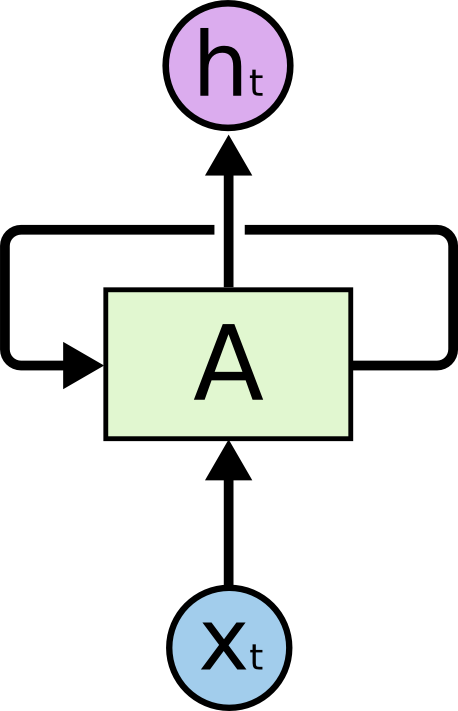
\includegraphics[width=0.2\linewidth]{Images//C5/RNN.png}
%         \vspace{0.5cm}
%         \caption{Recurrent Neural Network\\ Nguồn: https://colah.github.io, truy cập vào ngày 01/05/2025}
%     \end{figure}
%     Hình vẽ trên mô tả một đoạn của mạng nơ-ron hồi quy \textit{A} với đầu vào là $x_t$ và đầu ra là $h_t$ . Một vòng lặp cho phép thông tin có thể được truyền từ bước này qua bước này qua bước khác của mạng nơ-ron.\\
%     RNN cho phép duy trì một trạng thái ẩn (hidden state) được cập nhật liên tục theo thời gian, giúp lưu trữ thông tin từ các bước trước và sử dụng nó để xử lý bước hiện tại. Cụ thể, tại mỗi bước thời gian, RNN sẽ:
%     \begin{itemize}[label=--]
%         \item Nhận đầu vào hiện tại.
%         \item Kết hợp với trạng thái ẩn từ bước trước đó.
%         \item Tính toán trạng thái ẩn mới và đầu ra tương ứng
%     \end{itemize}
%     Nhờ cơ chế "hồi quy" này, RNN có khả năng nắm bắt mối quan hệ theo chuỗi và lưu trữ ngữ cảnh tạm thời, làm cho nó phù hợp với các bài toán thời gian thực hoặc dữ liệu tuần tự.\\
%     Tuy nhiên, RNN truyền thống vẫn gặp phải những hạn chế nghiêm trọng trong việc học các mối quan hệ dài hạn (long-term dependencies) do vấn đề vanishing gradient (gradient tiêu biến) khi huấn luyện. Để giải quyết vấn đề này, các kiến trúc nâng cao như LSTM và GRU đã được phát triển.
%     \item \textbf{Mạng LSTM}\\
%     Mạng bộ nhớ dài-ngắn (Long Short Term Memory networks), thường được gọi là LSTM - là một dạng đặc biệt của RNN, nó có khả năng học được các phụ thuộc xa. LSTM được thiết kế để tránh được vấn đề phụ thuộc xa (long-term dependency). Việc nhớ thông tin trong suốt thời gian dài là đặc tính mặc định của chúng, chứ không cần phải huấn luyện nó để có thể nhớ được. 
%     \begin{figure}[H]
%         \centering
%         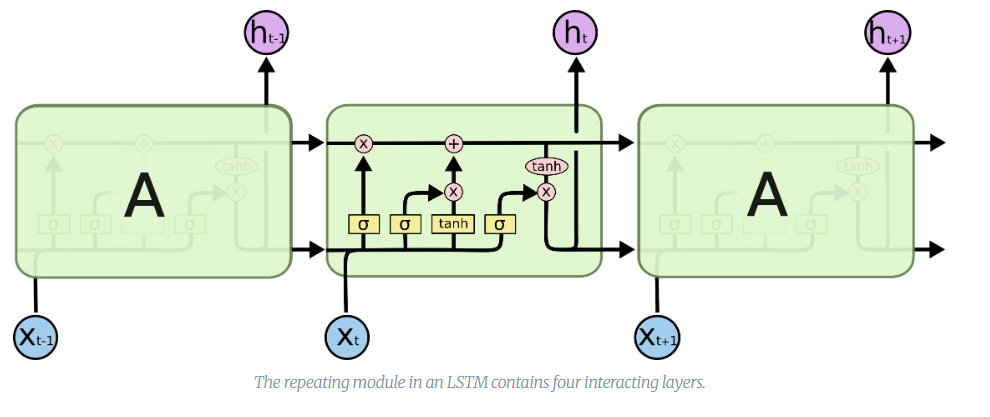
\includegraphics[width=0.75\linewidth]{Images//C5/LSTM.png}
%         \vspace{0.5cm}
%         \caption{Mạng LSTM\\ Nguồn: https://colah.github.io, truy cập vào ngày 01/05/2025}
%     \end{figure}
%     Cốt lõi của \textbf{LSTM} là \textit{cấu trúc ô nhớ (memory cell)} – nơi lưu trữ thông tin qua nhiều bước thời gian, kết hợp với ba cổng điều khiển chính (Các cổng là nơi sàng lọc thông tin đi qua nó, chúng được kết hợp bởi một tầng mạng sigmoid và một phép nhân):
%     \begin{itemize}[label=--]
%         \item Cổng vào (input gate): kiểm soát lượng thông tin mới được thêm vào ô nhớ.
%         \item Cổng quên (forget gate): quyết định thông tin nào trong ô nhớ cần được loại bỏ.
%         \item Cổng đầu ra (output gate): xác định thông tin nào sẽ được xuất ra tại bước hiện tại.
%     \end{itemize}
%     Nhờ các cơ chế này, LSTM có khả năng:
%     \begin{itemize}[label=--]
%         \item Ghi nhớ thông tin quan trọng trong thời gian dài.
%         \item Bỏ qua hoặc quên đi những thông tin không cần thiết.
%         \item Học hiệu quả các chuỗi dài mà không gặp vấn đề gradient tiêu biến như RNN.
%     \end{itemize}


% \end{enumerate}
% \subsection{Thiết kế}

% \subsubsection{Kiến trúc hệ thống}
% \noindent \textbf{Hệ thống quản lý tài sản CNTT theo thời gian thực} (Real-time IT Asset Management) được thiết kế để giám sát, quản lý và tối ưu hóa tài sản công nghệ thông tin. Kiến trúc hệ thống bao gồm nhiều thành phần chính để đảm bảo khả năng giám sát thời gian thực, lưu trữ dữ liệu hiệu quả, và hỗ trợ ra quyết định dựa trên phân tích dữ liệu. Hệ thống sẽ được thiết kế kết hợp giữa kiến trúc theo lớp.
% \begin{figure}[H]
%     \centering
%     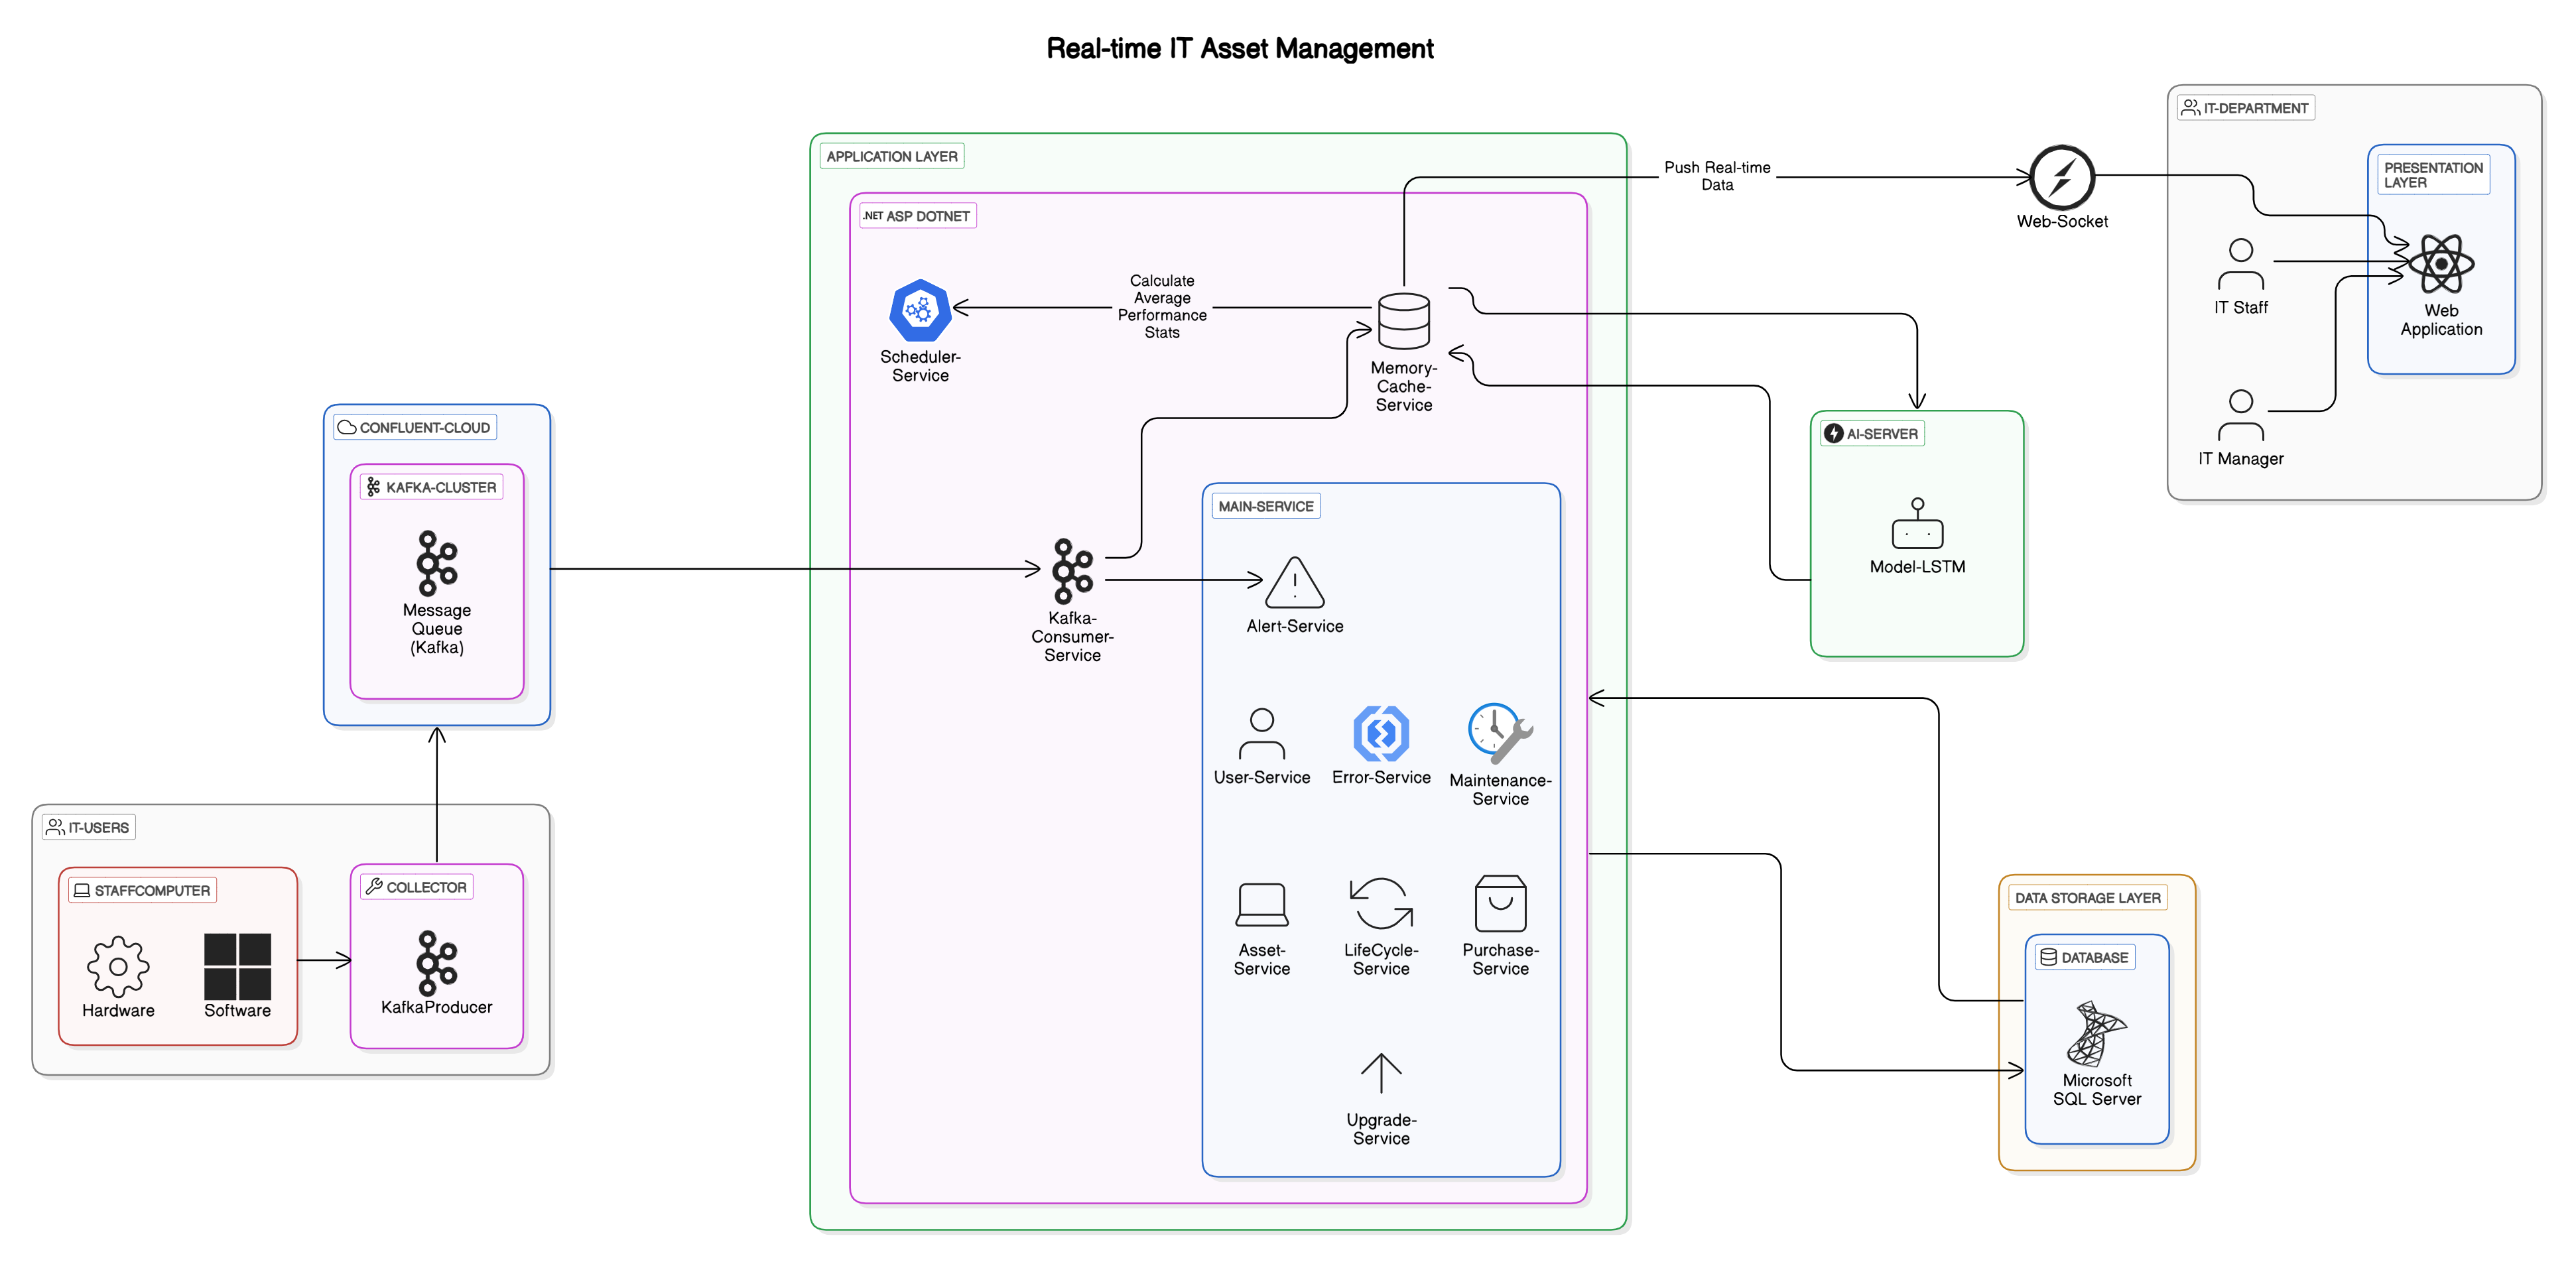
\includegraphics[width=\linewidth]{Images/C5/ITAM-Architecture.png}
%     \vspace{5pt}
%     \caption{Kiến trúc hệ thống ITAM}
% \end{figure}
% \noindent \textbf{Các thành phần chính của hệ thống}:
% \begin{enumerate}
%     \item \textbf{Bộ phận CNTT(IT Department)}:
%     \begin{itemize}[label=--]
%         \item Người dùng cuối là các nhân sự thuộc bộ phận IT, bao gồm:
%             \begin{itemize}[label=\textbullet]
%                 \item Nhân viên IT
%                 \item Quản lý
%             \end{itemize}
%         \item Cả hai đối tượng này tương tác với hệ thống qua \textbf{Presentation Layer} với Ứng dụng giao diện Web được phát triển bằng React.
%     \end{itemize}
%     \item \textbf{Tầng ứng dụng (Application Layer)}:\\
%     Tầng ứng dụng bao gồm các service:
%         \begin{itemize}[label=--]
%             \item Memory Cache Service: dùng để quản lý cache của hệ thống. Dữ liệu thời gian thực sẽ được cache lại với một khoảng thời gian nhất định.
%             \item Kafka Consumer Service: Dịch vụ chạy nền với vai trò là tiêu thụ tin nhắn từ Confluent Cloud
%             \item Scheduler Service: Dịch vụ chạy nền có vài trò là tính toán giá trị trung bình của hiệu suất mỗi ngày vào hai khung giờ là 10 giờ sáng và 14 giờ chiều.
%             \item Alert Service: dùng cho module cảnh báo
%             \item Life Cycle Service: dùng cho module quản lý vòng đời tài sản
%             \item Purchase Service: dùng cho module quản lý đơn đặt hàng
%             \item Upgrade Service: dùng để quản lý yêu cầu nâng cấp
%             \item Error \& Maintenance Service: dùng cho module quản lý sự cố và bảo trì            
%         \end{itemize}
%     \item \textbf{Tầng lưu trữ dữ liệu (Data Storage Layer) }:\\
%     Dữ liệu của hệ thống được lưu trữ trong Microsoft SQL Server, đảm bảo:
%     \begin{itemize}[label=--]
%         \item Quản lý dữ liệu liên quan đến tài sản.
%         \item Hỗ trợ lưu trữ dữ liệu về các sự kiện hệ thống.
%     \end{itemize}
%     \item \textbf{Người dùng tài sản CNTT (IT Users)}: \\
%     Tại mỗi máy của người dùng tài sản CNTT sẽ cài đặt Collector. Collector có trách nhiệm thu thập thông tin cấu hình phần cứng, phần mềm tại mỗi máy tính. Collector này đóng vai trò là Producer.
%     \item \textbf{AI Server}: Dùng để dự đoán hiệu suất tài sản
%     \item \textbf{Websocker}: Dùng để truyền dữ liệu theo thời gian thực
% \end{enumerate}
%     \textbf{Dữ liệu thu thập từ người dùng tài sản CNTT}: 
%     \begin{enumerate}
%         \item Dữ liệu từ phần cứng, phần mềm được thu thập qua Collector. \item Kafka Producer hay Collector sau đó đẩy dữ liệu lên Confluent Cloud
%         \item Dữ liệu này được Kafka Consumer Service tiêu thụ và lưu tại cache
%         \item Dữ liệu sau đó sẽ được xử lý tại các service, sau khi xử lý xong sẽ được truyền đến giao diện bằng WebSocket.
%     \end{enumerate}
% \subsubsection{Thiết kế cơ sở dữ liệu}
% \begin{figure}[H]
%     \centering
%     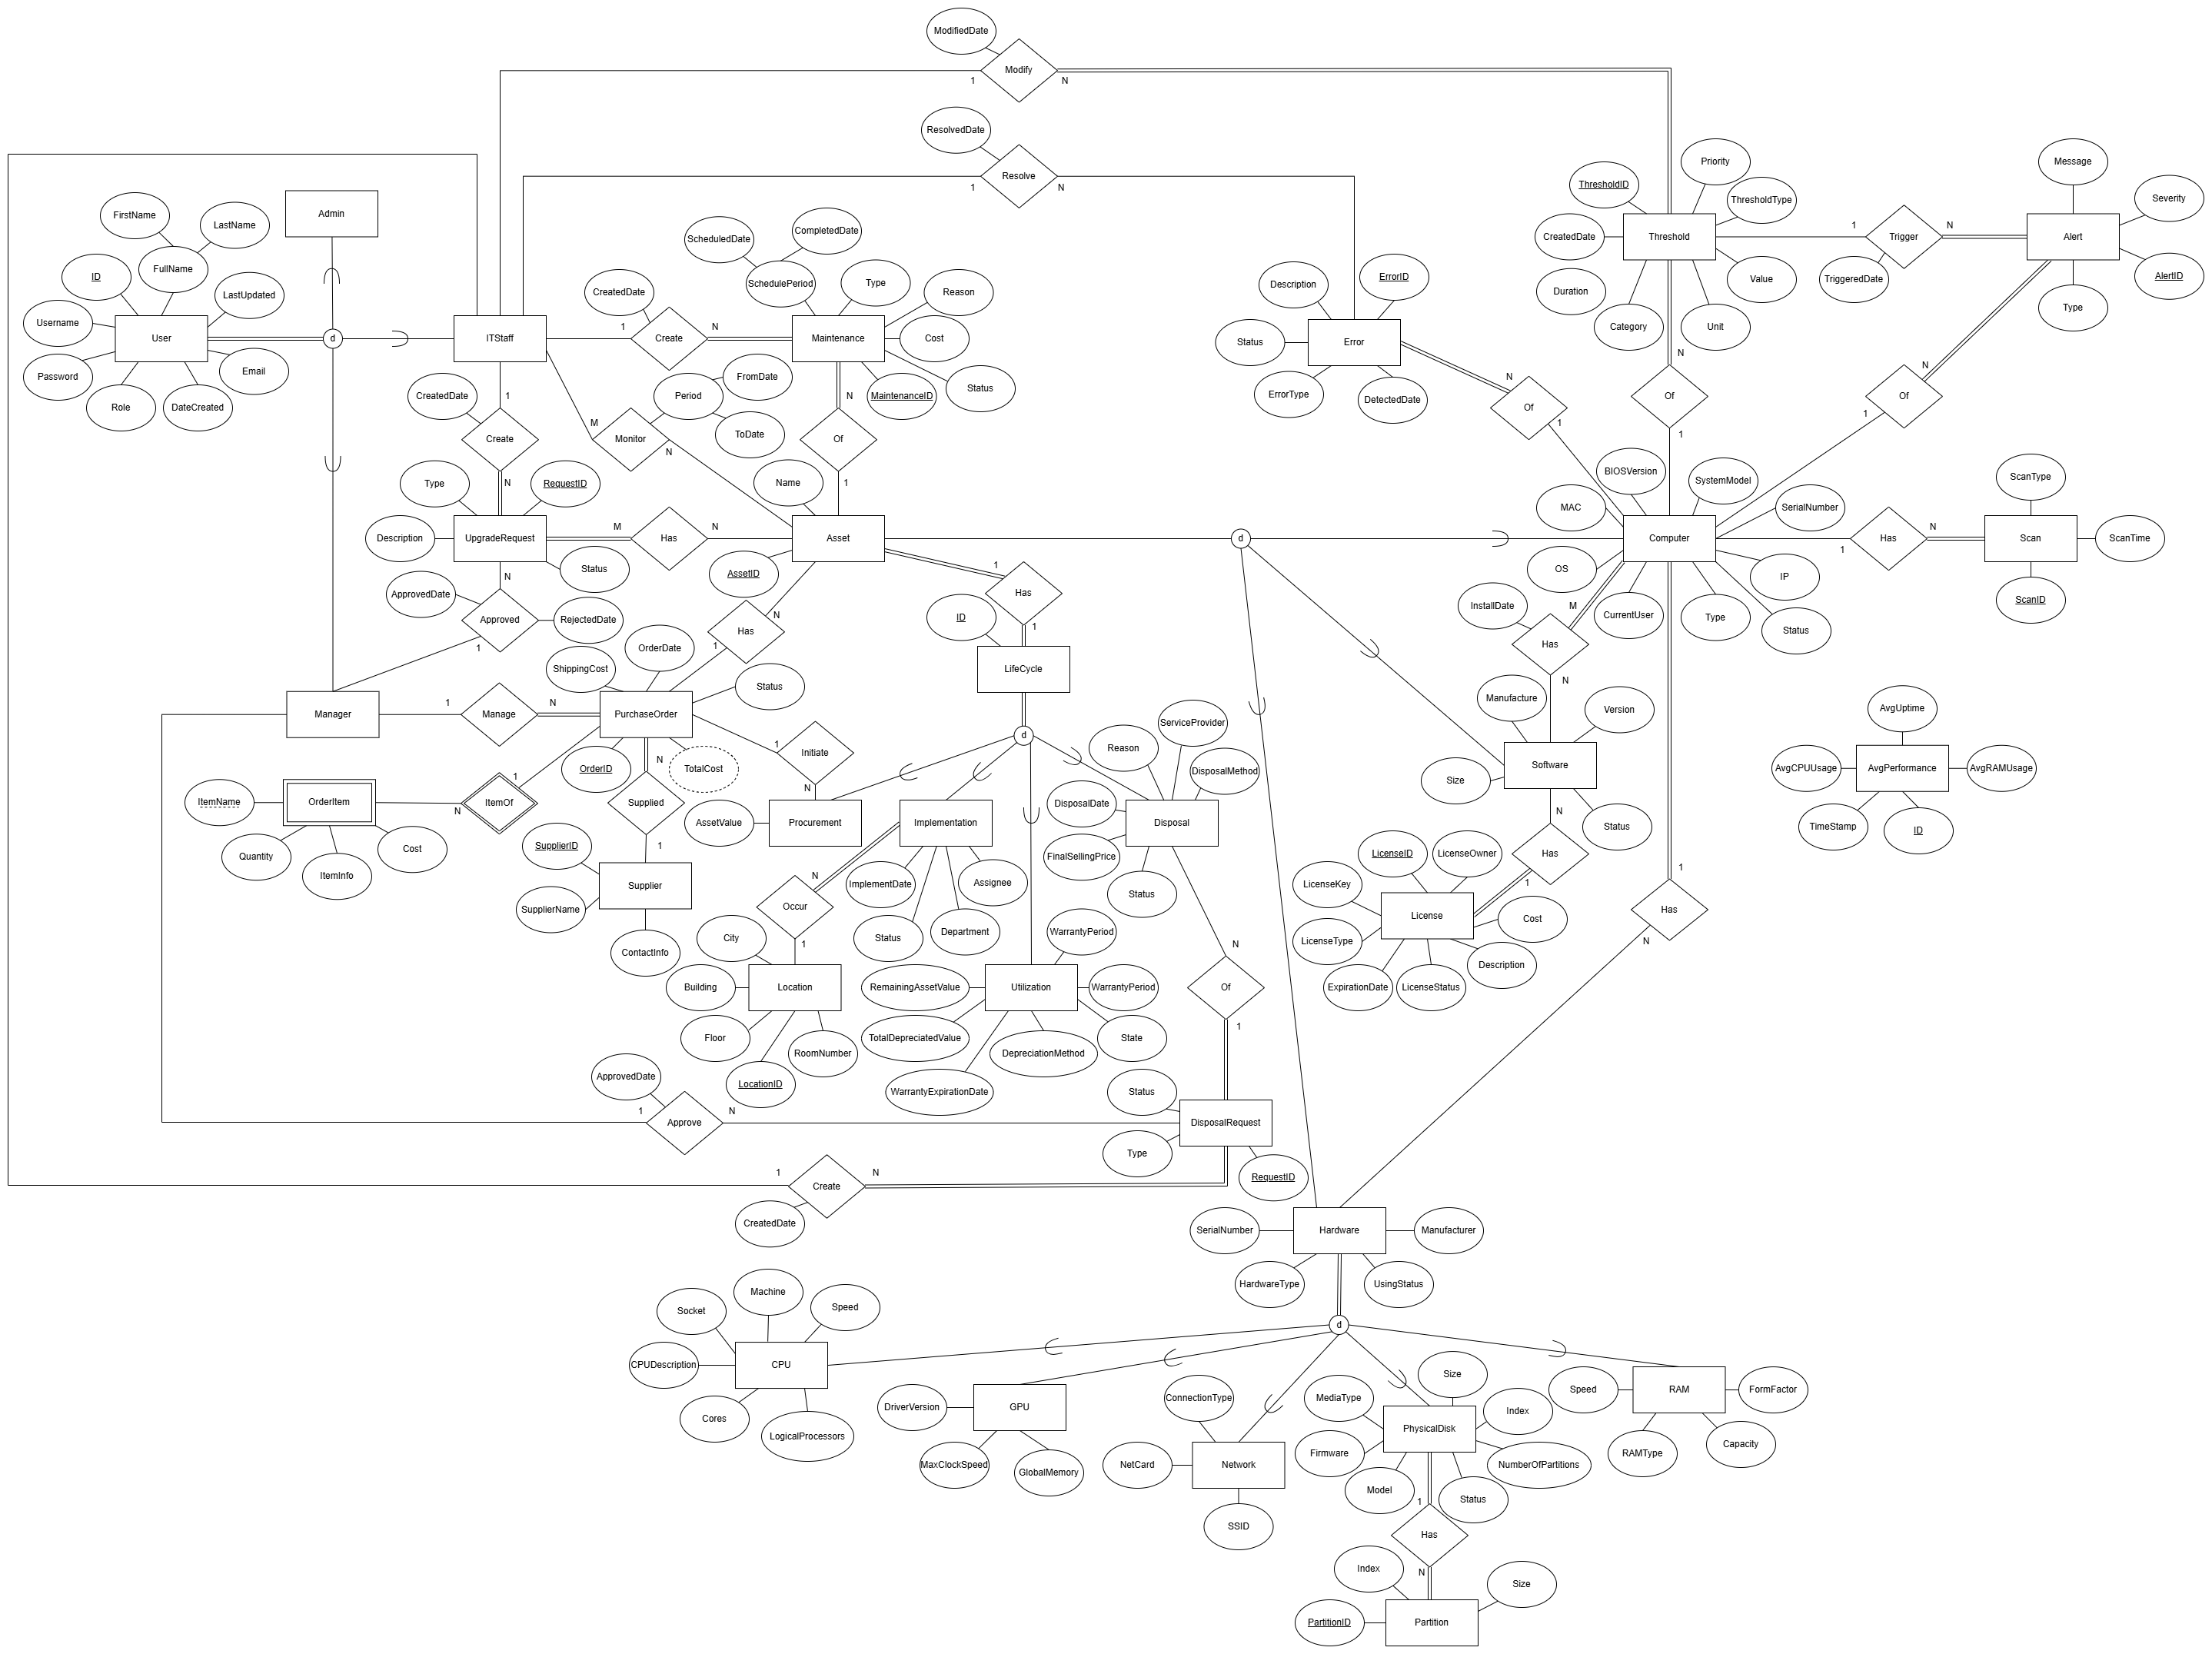
\includegraphics[width=\linewidth]{Images/C5/EERD.png}
%     \vspace{5pt}
%     \caption{Enhanced Entity-Relationship Diagram}
% \end{figure}
% \noindent \textbf{Các thành phần chính của EERD:}
% \begin{enumerate}
%     \item Thực thể (Entities)
%     \begin{itemize}[label=--]
%         \item Asset (Tài sản): Thực thể trung tâm trong hệ thống quản lý tài sản ITAM, đại diện cho mọi tài sản công nghệ thông tin trong tổ chức, bao gồm cả phần cứng, phần mềm và máy tính.
%         \item Hardware (Phần cứng): Là thực thể con của Asset, đại diện cho các tài sản vật lý thuộc về CNTT. Bao gồm nhiều thành phần phần cứng cụ thể như:
%         \begin{itemize}[label=\textbullet]
%             \item CPU: Đại diện cho bộ xử lý trung tâm của máy tính.
%             \item GPU: Đại diện cho bộ xử lý đồ họa trong hệ thống.
%             \item RAM: Đại diện cho bộ nhớ truy cập ngẫu nhiên của máy tính.
%             \item PhysicalDisk: Đại diện cho ổ đĩa vật lý được sử dụng để lưu trữ dữ liệu.
%             \item Network: Đại diện cho thiết bị mạng như card mạng và các kết nối mạng liên quan.
%         \end{itemize}
%         \item Partition (Phân vùng): Là thành phần liên quan đến PhysicalDisk, đại diện cho các phân vùng được tạo trên ổ đĩa vật lý.
%         \item Software (Phần mềm): Là thực thể con của Asset, đại diện cho các ứng dụng, phần mềm hệ thống hoặc phần mềm cài đặt trên các thiết bị.
%         \item Computer (Máy tính): Là thực thể con khác của Asset, đại diện cho các thiết bị máy tính cá nhân hoặc máy bàn, có mối quan hệ với cả các thành phần phần cứng và phần mềm được cài đặt trên máy.
%         \item License (Giấy phép): Đại diện cho các thông tin về bản quyền, thời hạn sử dụng và điều khoản liên quan đến các phần mềm thuộc tài sản.
%         \item Supplier (Nhà cung cấp): Đại diện cho các đơn vị cung cấp tài sản CNTT, phần mềm hoặc dịch vụ bảo trì liên quan.
%         \item PurchaseOrder (Đơn đặt hàng): Đại diện cho các đơn đặt hàng được tạo ra để mua sắm tài sản CNTT từ nhà cung cấp.
%         \item OrderItem (Thành phần của đơn đặt hàng): Các thành phần thông tin về tài sản cụ thể khi quản lý tạo và gửi yêu cầu đặt hàng đến với nhà cung cấp.
%         \item Threshold (Ngưỡng cảnh báo): Ghi nhận các ngưỡng cảnh báo do nhân viên cài đặt đối với từng máy tính để có thể giám sát, theo dõi và cảnh báo khi có thông số cao hoặc thấp của các tài sản liên quan đến máy tính này.
%         \item Alert (Cảnh báo): Thực thể này ghi nhận các cảnh báo liên quan đến tài sản của máy tính vượt ngưỡng cảnh báo.
%         \item Error (Lỗi): Ghi nhận các lỗi xảy ra trong quá trình thu thập dữ liệu tài sản từ collector.
%         \item  Maintenance (Bảo trì): Ghi lại các sự kiện bảo trì hoặc sửa chữa tài sản.
%         \item Upgrade Request (Yêu cầu nâng cấp): Thực thể này ghi nhận các yêu cầu nâng cấp liên quan đến một hay nhiều tài sản công nhận thông tin mà nhân viên IT sẽ đề xuất lên cho quản lý để được phê duyệt.
%         \item User (Người dùng): Thực thể cha đại diện cho các nhóm người dùng trong hệ thống.
%         \begin{itemize}[label=\textbullet]
%             \item System Administrator (Quản trị viên hệ thống): Thực thể con của User, có quyền cao nhất có toàn quyền quyết định đối với hệ thống.
%             \item IT Staff (Nhân viên IT): Quản lý và theo dõi các tài sản cụ thể, không có quyền thay đổi đơn đặt hàng.
%             \item Manager (Quản lý): Phê duyệt đơn đặt hàng và xem các báo cáo tài sản, nhưng không có quyền thay đổi cấu hình hệ thống.
%         \end{itemize}
%         \item LifeCycle (Vòng đời tài sản): Đại diện cho các giai đoạn mà một tài sản CNTT trải qua, bao gồm:
%         \begin{itemize}[label=\textbullet]
%             \item Procurement: Giai đoạn mua sắm tài sản.
%             \item Implementation: Giai đoạn cài đặt, thiết lập và triển khai sử dụng tài sản.
%             \item Utilization: Giai đoạn tài sản được đưa vào sử dụng thường xuyên trong hoạt động của tổ chức.
%             \item Disposal: Giai đoạn tài sản bị loại bỏ, thanh lý hoặc ngừng sử dụng.
%         \end{itemize}
%         \item Location (Vị trí): Đại diện cho vị trí vật lý hoặc bộ phận trong tổ chức mà tài sản được phân bổ và sử dụng.
%         \item DisposalRequest (Yêu cầu thanh lý): Ghi nhận các yêu cầu thanh lý tài sản từ nhân viên đến quản lý để thực hiện quy trình loại bỏ hợp lệ.
%         \item Scan (Quét): Đại diện cho các hoạt động quét tự động để thu thập dữ liệu tài sản từ máy tính hoặc hệ thống.
%         \item AvgPerformance (Hiệu suất trung bình): Là thực thể ghi nhận các chỉ số hiệu suất tổng hợp của tài sản, đặc biệt là máy tính, nhằm phục vụ việc giám sát và đánh giá.
%     \end{itemize}
%     \item Tổng hợp/Phân loại (Generalization/Specialization)
%     \begin{itemize}[label=--]
%         \item User (Người dùng): Là một tổng thể được phân loại thành các nhóm người dùng khác nhau, cụ thể như sau:
%         \begin{itemize}[label=\textbullet]
%             \item \textbf{Disjoint}: Một người dùng chỉ thuộc duy nhất một nhóm (không thể vừa là quản trị viên vừa là nhân viên IT).
%             \item \textbf{Total}: Mọi người dùng trong hệ thống đều phải thuộc một trong các nhóm sau: System Administrator (Quản trị viên hệ thống), IT Staff (Nhân viên IT), Manager (Quản lý).
%         \end{itemize}
%         \item Asset (Tài sản): Là thực thể tổng quát được phân loại thành ba loại tài sản cụ thể:
%         \begin{itemize}[label=\textbullet]
%             \item \textbf{Disjoint}: Mỗi tài sản chỉ thuộc duy nhất một loại (không thể vừa là phần mềm vừa là máy tính).
%             \item Total: Mọi tài sản trong hệ thống đều phải là một trong ba nhóm sau:Hardware (Phần cứng), Software (Phần mềm), Computer (Máy tính).
%         \end{itemize}
%         \item Hardware (Phần cứng): Là thực thể con của Asset, được phân loại thêm thành các thành phần phần cứng cụ thể:
%         \begin{itemize}[label=\textbullet]
%             \item \textbf{Disjoint}: Một phần cứng chỉ thuộc một loại duy nhất (ví dụ: một phần cứng không thể vừa là RAM vừa là GPU).
%             \item \textbf{Partial}: Không phải mọi phần cứng đều nhất thiết phải thuộc một trong các nhóm hiện tại, cho phép mở rộng thêm các loại phần cứng khác trong tương lai.
%             \item Các nhóm hiện tại bao gồm: CPU, GPU, RAM, PhysicalDisk, Network.
%         \end{itemize}
%         \item LifeCycle là một thực thể tổng quát mô tả toàn bộ vòng đời mà một tài sản CNTT phải trải qua, được phân loại thành các giai đoạn cụ thể:
%         \begin{itemize}[label=\textbullet]
%             \item \textbf{Disjoint}: Mỗi trạng thái cụ thể của vòng đời là tách biệt — một tài sản tại một thời điểm chỉ có thể nằm trong một giai đoạn vòng đời duy nhất.
%             \item \textbf{Total}: Mọi tài sản đều phải nằm trong một giai đoạn của vòng đời tại mọi thời điểm.
%             \item Các giai đoạn cụ thể bao gồm: Procurement (Mua sắm), Implementation (Triển khai), Utilization (Sử dụng), Disposal (Thanh lý).
%         \end{itemize}
%     \end{itemize}
%     \item Phân quyền (Authorization Levels) \\
%     Sự phân quyền giữa các nhóm người dùng được biểu diễn qua các mối quan hệ với các thực thể khác. Quyền hạn sẽ khác nhau tùy vào nhóm người dùng cụ thể, từ quản lý toàn bộ đến chỉ xem hoặc phê duyệt.
% \end{enumerate}
% \subsubsection{ Thiết kế chi tiết bên trong}
% \begin{figure}[H]
%     \centering
%     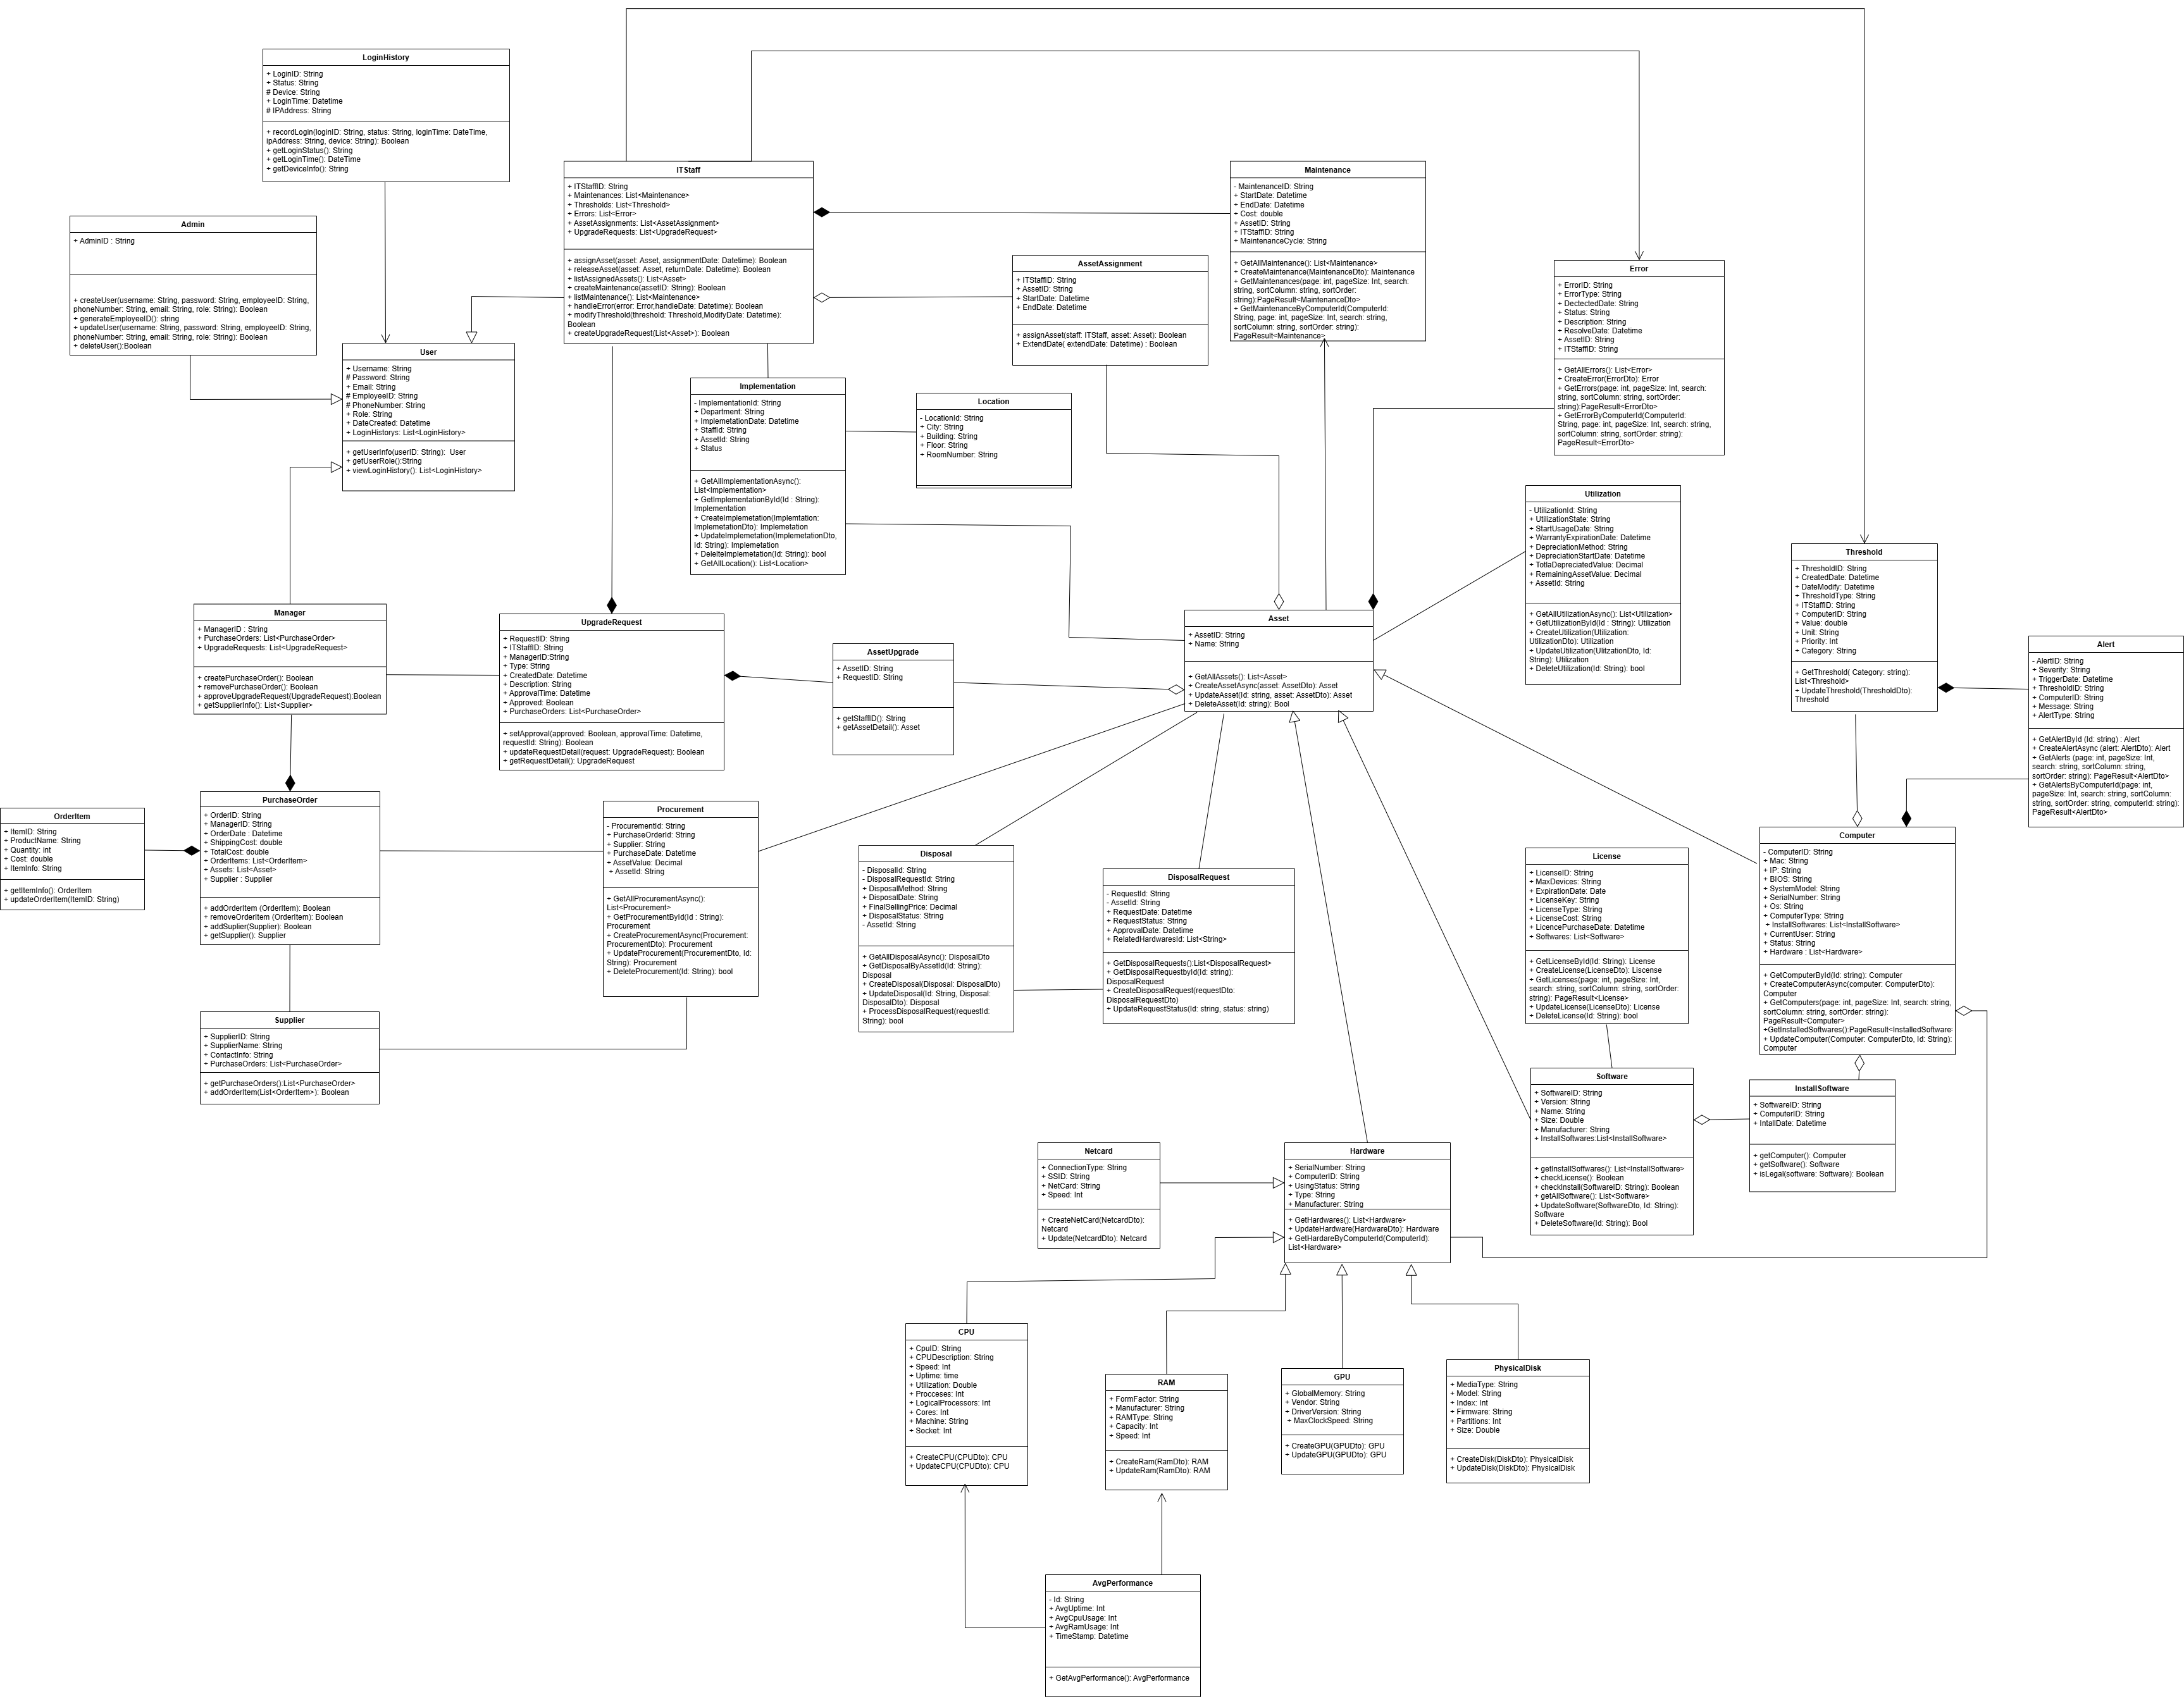
\includegraphics[width=\linewidth]{Images/C5/ClassDiagram.png}
%     \vspace{5pt}
%     \caption{Class Diagram}
% \end{figure}
% \subsection{Thiết kế API}
% \noindent Dưới đây là trình bày chi tiết thiết kế các giao diện lập trình ứng dụng (API) được sử dụng trong hệ thống. Thiết kế đầy đủ của toàn bộ hệ thống được trình bày tại đây \href{https://app.swaggerhub.com/apis/ITAMhcmut/APIDesign/1.0.0}{Link}.
% \subsubsection{Quản lý người dùng}
%     \begin{enumerate}
%         \item \textbf{Đăng nhập}
%         \begin{itemize}[label=--]
%             \item \textbf{URL:} \texttt{/api/login}
%             \item \textbf{Method:} POST
%             \item \textbf{Description:} API dùng để xác thực thông tin đăng nhập của người dùng.            
%             \item \textbf{Authorization:}
%             \begin{itemize}[label=\textbullet]
%                 \item Yêu cầu: Không yêu cầu
%                 \item Quyền truy cập: Mọi người dùng đều có thể gọi API này để đăng nhập.
%             \end{itemize}
%             \item \textbf{Request:} 
%             \begin{itemize}[label=\textbullet]
%                 \item Content-Type: \texttt{application/json}
%                 \item Request Body:
%             \end{itemize}
%             \begin{longtable}{|l|l|l|l|}
%             \hline
%             \textbf{Trường} & \textbf{Kiểu} & \textbf{Mô tả} & \textbf{Bắt buộc} \\
%             \hline
%             \endhead
%             \texttt{email} & String & Địa chỉ email người dùng & Có \\
%             \texttt{password} & String & Mật khẩu đăng nhập & Có \\
%             \hline
%             \end{longtable}
%             \item \textbf{Responses:}
%             \begin{itemize}[label=\textbullet]
%                 \item \textbf{200 OK:} Đăng nhập thành công. Dữ liệu JSON trả về:
%                 \begin{longtable}{|l|l|l|}
%                 \hline
%                 \textbf{Trường} & \textbf{Kiểu} & \textbf{Mô tả} \\
%                 \hline
%                 \endhead
%                 \texttt{accessToken} & String & Token JWT dùng để xác thực truy cập \\
%                 \hline
%                 \texttt{refreshToken} & String & Token để làm mới \texttt{accessToken}\\
%                 \hline
%                 \end{longtable}
%                 \item \textbf{500 Internal Server Error:} Có lỗi xảy ra trong quá trình xử lý hoặc người dùng không được phép đăng nhập. Không có dữ liệu trả về.
%             \end{itemize}
%         \end{itemize}
%         \item \textbf{Truy vấn thông tin của người dùng}
%         \begin{itemize}[label=--]
%             \item \textbf{URL:} \texttt{/api/users/\{id\}}
%             \item \textbf{Method:} GET
%             \item \textbf{Description:} Lấy thông tin chi tiết của người dùng cụ thể dựa trên \texttt{id}.            
%             \item \textbf{Authorization:}
%             \begin{itemize}[label=\textbullet]
%                 \item Yêu cầu: Header Authorization: Bearer <\texttt{accessToken}>
%                 \item Quyền truy cập: Administrator, Manager
%                 \item Phản hồi nếu không đủ quyền: 403 Forbidden
%             \end{itemize}
%             \item \textbf{Parameters:}
%             \begin{longtable}{|l|l|l|l|l|}
%             \hline
%             \textbf{Tên tham số} & \textbf{Vị trí} & \textbf{Kiểu dữ liệu} & \textbf{Bắt buộc} & \textbf{Mô tả} \\
%             \hline
%             \endhead
%             \texttt{id} & Path & String & Có & ID của người dùng\\
%             \hline
%             \end{longtable}
%             \item \textbf{Responses:}
%             \begin{itemize}[label=\textbullet]
%                 \item \textbf{200 OK:} Lấy thông tin thành công. Trả về dữ liệu chi tiết của người dùng.
%                 \begin{longtable}{|l|l|l|}
%                 \hline
%                 \textbf{Trường} & \textbf{Kiểu} & \textbf{Mô tả} \\
%                 \hline
%                 \endhead
%                 \texttt{id} & String & ID của người dùng \\
%                 \texttt{firstName} & String & Họ của người dùng \\
%                 \texttt{lastName} & String & Tên của người dùng \\
%                 \texttt{role} & String & Vai trò của người dùng \\
%                 \texttt{phoneNumber} & String & Số điện thoại người dùng \\
%                 \texttt{createdAt} & String & Ngày tạo tài khoản (ISO format) \\
%                 \texttt{lastUpdatedAt} & String & Ngày cập nhật gần nhất \\
%                 \texttt{accessToken} & String & Token xác thực truy cập \\
%                 \texttt{refreshToken} & String & Token làm mới \\                
%                 \hline
%                 \end{longtable}
%                 \item \textbf{403 Forbidden:} Người dùng không có quyền truy cập tài nguyên này. Không có dữ liệu trả về.
%                 \item \textbf{500 Internal Server Error} - Có lỗi xảy ra trong quá trình truy vấn người dùng. Không có dữ liệu trả về 
%             \end{itemize}
%         \end{itemize}
%     \end{enumerate}
% \subsubsection{Quản lý tài sản}
%     \begin{enumerate}
%         \item \textbf{Tạo mới máy tính}
%         \begin{itemize}[label=--]
%             \item \textbf{URL:} \texttt{/api/computer/CreateComputer}
%             \item \textbf{Method:} POST
%             \item \textbf{Description:} Tạo mới một tài sản máy tính
%             \item \textbf{Authorization:}
%             \begin{itemize}[label=\textbullet]
%                 \item Yêu cầu: Authorization: Bearer <\texttt{accessToken}>
%                 \item Quyền truy cập: Administrator, ITStaff
%                 \item Phản hồi nếu không đủ quyền: 403 Forbidden
%             \end{itemize}
%             \item \textbf{Request:}
%             \begin{itemize}[label=\textbullet]
%                 \item Content-Type: \texttt{application/json}
%                 \item Request Body:
%             \end{itemize}
%             \begin{longtable}{|l|l|l|l|}
%             \hline
%             \textbf{Trường} & \textbf{Kiểu} & \textbf{Mô tả} & \textbf{Bắt buộc} \\
%             \hline
%             \endhead
%             \texttt{name} & String & Tên thiết bị (do người dùng đặt) & Có \\
%             \texttt{model} & String & Model của máy tính & Không \\
%             \texttt{serialNumber} & String & Số serial & Không \\
%             \texttt{os} & String & Hệ điều hành & Không \\
%             \texttt{computerType} & String & Loại máy tính (Laptop, Desktop) & Có \\
%             \hline
%             \end{longtable}
%             \item \textbf{Responses:}
%             \begin{itemize}[label=\textbullet]
%                 \item \textbf{200 OK:} Tạo thành công. Trả về thông tin chi tiết của máy tính vừa được tạo. 
%                 \begin{longtable}{|l|l|l|}
%                 \hline
%                 \textbf{Trường} & \textbf{Kiểu} & \textbf{Mô tả} \\
%                 \hline
%                 \endhead
%                 \texttt{assetId} & String & Mã định danh của thiết bị \\
%                 \texttt{name} & String & Tên thiết bị \\
%                 \texttt{mac} & String & Địa chỉ MAC \\
%                 \texttt{ip} & String & Địa chỉ IP \\
%                 \texttt{bios} & String & Thông tin BIOS \\
%                 \texttt{model} & String & Model thiết bị \\
%                 \texttt{serialNumber} & String & Số serial \\
%                 \texttt{os} & String & Hệ điều hành \\
%                 \texttt{computerType} & String & Loại máy tính \\
%                 \texttt{currentUser} & String & Người dùng hiện tại \\
%                 \texttt{status} & String & Trạng thái thiết bị \\
%                 \texttt{hardware} & Array[Object] & Thông tin phần cứng chi tiết \\
%                 \hline
%                 \end{longtable}
%                 \item \textbf{403 Forbidden:} Người dùng không có quyền tạo máy tính. Không có dữ liệu trả về.
%                 \item \textbf{500 Internal Server Error:} Dữ liệu đầu vào không hợp lệ hoặc có lỗi trong quá trình xử lý. Không có dữ liệu trả về.
%             \end{itemize}
%         \end{itemize}
%         \item \textbf{Truy vấn thông tin phần cứng}
%         \begin{itemize}[label=--]
%             \item \textbf{URL:} \texttt{/api/hardware/GetHardwares}
%             \item \textbf{Method:} GET
%             \item \textbf{Description:} API này dùng để truy vấn danh sách phần cứng từ hệ thống, hỗ trợ phân trang, tìm kiếm và sắp xếp.
%             \item \textbf{Authorization:}
%             \begin{itemize}[label=\textbullet]
%                 \item Yêu cầu: Header Authorization: Bearer <\texttt{accessToken}>.
%                 \item Quyền truy cập: Administrator, Manager, ITStaff.
%                 \item Phản hồi nếu không đủ quyền: 403 Forbidden.
%             \end{itemize}
%             \item \textbf{Parameters:}
%             \begin{longtable}{|l|l|l|l|l|}
%             \hline
%             \textbf{Tên tham số} & \textbf{Vị trí} & \textbf{Kiểu} & \textbf{Bắt buộc} & \textbf{Mô tả} \\
%             \hline
%             \endhead
%             \texttt{page} & Query & Number & Không & Số trang hiện tại\\
%             \texttt{pageSize} & Query & Number & Không & Số phần tử mỗi trang \\
%             \texttt{search} & Query & String & Không & Từ khóa tìm kiếm\\
%             \texttt{sortColumn} & Query & String & Không & 	Cột dùng để sắp xếp \\
%             \texttt{sortOrder} & Query & String & Không & \texttt{asc} hoặc \texttt{desc}\\
%             \hline
%             \end{longtable}
%             \item \textbf{Responses:}
%             \begin{itemize}[label=\textbullet]
%                 \item \textbf{200 OK:} Lấy dữ liệu thành công. Trả về danh sách phần cứng và thông tin phân trang.
%                 \begin{longtable}{|l|l|l|}
%                 \hline
%                 \textbf{Trường} & \textbf{Kiểu} & \textbf{Mô tả} \\
%                 \hline
%                 \endhead
%                 \texttt{items} & Array[Object] & Danh sách phần cứng\\
%                 \texttt{totalRecords} & Number & Tổng số phần cứng trong hệ thống \\
%                 \texttt{currentPage} & Number & Trang hiện tại \\
%                 \texttt{pageSize} & Number & Số phần tử mỗi trang \\
%                 \texttt{totalPages} & Number & Tổng số trang \\
%                 \hline
%                 \end{longtable}
%                 Mỗi phần tử trong \texttt{items} sẽ là một object phần cứng, bao gồm:
%                 \begin{longtable}{|l|l|l|}
%                 \hline
%                 \textbf{Trường} & \textbf{Kiểu} & \textbf{Mô tả} \\
%                 \hline
%                 \endhead
%                 \texttt{serialNumber} & String & Số serial của phần cứng \\
%                 \texttt{computerID} & String & ID máy tính đang gắn phần cứng \\
%                 \texttt{hardwareType} & String & Loại phần cứng \\
%                 \texttt{usingStatus} & String & Trạng thái sử dụng \\
%                 \texttt{manufacturer} & String & Hãng sản xuất \\
%                 \texttt{details} & String & Thông tin chi tiết \\
%                 \texttt{assetId} & String & Mã định danh tài sản liên quan \\
%                 \texttt{name} & String & Tên định danh của phần cứng trong hệ thống \\
%                 \hline
%                 \end{longtable}
%                 \item \textbf{403 Forbidden:} Người dùng không có quyền truy cập API. Không có dữ liệu trả về.
%                 \item \textbf{500 Internal Server Error:} Dữ liệu đầu vào không hợp lệ hoặc có lỗi trong quá trình xử lý. Không có dữ liệu trả về.
%             \end{itemize}
%         \end{itemize}
%     \end{enumerate}
% \subsubsection{Yêu cầu nâng cấp tài sản}
%     \begin{enumerate}
%         \item \textbf{Tạo yêu cầu nâng cấp phần mềm}
%         \begin{itemize}[label=--]
%             \item \textbf{URL:} \texttt{/api/UpgradeRequest/software}
%             \item \textbf{Method:} POST
%             \item \textbf{Description:} API dùng để tạo mới một yêu cầu nâng cấp phần mềm cho thiết bị (tài sản).
%             \item \textbf{Authorization:}
%             \begin{itemize}[label=\textbullet]
%                 \item Yêu cầu: Header Authorization: Bearer <\texttt{accessToken}>.
%                 \item Quyền truy cập: Administrator, ITStaff.
%                 \item Phản hồi nếu không đủ quyền: 403 Forbidden.
%             \end{itemize}
%             \item \textbf{Request:}
%             \begin{itemize}[label=\textbullet]
%                 \item Content-Type: \texttt{application/json}
%                 \item Request Body:
%             \end{itemize}
%             \begin{longtable}{|l|l|l|l|}
%             \hline
%             \textbf{Trường} & \textbf{Kiểu} & \textbf{Mô tả} & \textbf{Bắt buộc} \\
%             \hline
%             \endhead
%             \texttt{description} & String & Mô tả ngắn gọn yêu cầu nâng cấp & Không \\
%             \texttt{updateReason} & String & Lý do cần nâng cấp phần mềm & Không \\
%             \texttt{assetId} & String & ID của thiết bị & Có \\
%             \texttt{updateType} & String & Loại cập nhật & Có \\
%             \texttt{managerName} & String & Tên người quản lý phê duyệt & Có \\
%             \texttt{staffName} & String & Tên nhân viên tạo yêu cầu & Có \\
%             \texttt{softwareType} & String & Loại phần mềm yêu cầu nâng cấp & Có\\
%             \texttt{softwareAlt} & String & ID của phần mềm nâng cấp & Có \\
%             \hline
%             \end{longtable}
%             \item \textbf{Responses:}
%             \begin{itemize}[label=\textbullet]
%                 \item \textbf{200 OK:} Tạo yêu cầu thành công. Trả về thông tin của yêu cầu nâng cấp vừa tạo.
%                 \begin{longtable}{|l|l|l|}
%                 \hline
%                 \textbf{Trường} & \textbf{Kiểu} & \textbf{Mô tả} \\
%                 \hline
%                 \endhead
%                 \texttt{requestId} & String & ID của yêu cầu nâng cấp \\
%                 \texttt{staffName} & String & Tên nhân viên gửi yêu cầu \\
%                 \texttt{managerName} & String & Tên người quản lý sẽ phê duyệt hoặc từ chối yêu cầu \\
%                 \texttt{createdDate} & String & Ngày tạo yêu cầu (ISO Format) \\
%                 \texttt{approvedDate} & String & Ngày yêu cầu được phê duyệt (nếu có) \\
%                 \texttt{rejectedDate} & String & Ngày yêu cầu bị từ chối (nếu có) \\
%                 \texttt{status} & String & Trạng thái hiện tại của yêu cầu \\
%                 \texttt{description} & String & Mô tả nội dung yêu cầu \\
%                 \texttt{updateReason} & String & Lý do đề xuất nâng cấp phần mềm \\
%                 \texttt{updateType} & String & Loại nâng cấp \\
%                 \texttt{typeDetail} & String & Thông tin chi tiết hơn về phần mềm cần nâng cấp \\
%                 \hline
%                 \end{longtable}
%                 \item \textbf{403 Forbidden:} Người dùng không có quyền truy cập API. Không có dữ liệu trả về.
%                 \item \textbf{500 Internal Server Error:} Dữ liệu đầu vào không hợp lệ hoặc có lỗi trong quá trình xử lý. Không có dữ liệu trả về.
%             \end{itemize}
%         \end{itemize}
%         \item \textbf{Hủy yêu cầu nâng cấp}
%         \begin{itemize}[label=--]
%             \item \textbf{URL:} \texttt{/api/UpgradeRequest/cancel/\{id\}}
%             \item \textbf{Method:} PUT
%             \item \textbf{Description:} Hủy một yêu cầu nâng cấp chưa được xử lý (trạng thái còn Pending).
%             \item \textbf{Authorization:}
%             \begin{itemize}[label=\textbullet]
%                 \item Yêu cầu: Header Authorization: Bearer <\texttt{accessToken}>.
%                 \item Quyền truy cập: Administrator, ITStaff.
%                 \item Phản hồi nếu không đủ quyền: 403 Forbidden.                
%             \end{itemize}
%             \item \textbf{Parameters:}
%             \begin{longtable}{|l|l|l|l|l|}
%             \hline
%             \textbf{Tên tham số} & \textbf{Vị trí} & \textbf{Kiểu} & \textbf{Bắt buộc} & \textbf{Mô tả} \\
%             \hline
%             \endhead
%             \texttt{id} & Path & String & Có & ID của yêu cầu cần hủy \\
%             \hline
%             \end{longtable}
%             \item \textbf{Responses:}
%             \begin{itemize}[label=\textbullet]
%                 \item \textbf{200 OK:} Hủy yêu cầu thành công. Trả về thông tin của yêu cầu đã cập nhật trạng thái.
%                 \item \textbf{403 Forbidden:} Người dùng không có quyền truy cập API. Không có dữ liệu trả về.
%                 \item \textbf{500 Internal Server Error:} Dữ liệu đầu vào không hợp lệ hoặc có lỗi trong quá trình xử lý. Không có dữ liệu trả về.
%             \end{itemize}
%         \end{itemize}
%     \end{enumerate}
% \subsubsection{Quản lý đơn đặt hàng}
%     \begin{enumerate}
%         \item \textbf{Tạo mới đơn đặt hàng}
%         \begin{itemize}[label=--]
%             \item \textbf{URL:} \texttt{/api/purchase-order/new}
%             \item \textbf{Method:} POST
%             \item \textbf{Description:} API dùng để tạo mới một đơn mua hàng với thông tin nhà cung cấp, các mặt hàng và chi phí liên quan.
%             \item \textbf{Authorization:}
%             \begin{itemize}[label=\textbullet]
%                 \item Yêu cầu: Header Authorization: Bearer <\texttt{accessToken}>.
%                 \item Quyền truy cập: Administrator, Manager
%                 \item Phản hồi nếu không đủ quyền: 403 Forbidden.
%             \end{itemize}
%             \item \textbf{Request:}
%             \begin{itemize}[label=\textbullet]
%                 \item Content-Type: \texttt{application/json}
%                 \item Request Body:
%             \end{itemize}
%             \begin{longtable}{|l|l|l|l|}
%             \hline
%             \textbf{Trường} & \textbf{Kiểu} & \textbf{Mô tả} & \textbf{Bắt buộc} \\
%             \hline
%             \endhead
%             \texttt{orderDate} & String &  Ngày tạo đơn (ISO Format) & Có  \\
%             \texttt{shippingCost} & Number & Chi phí vận chuyển & Có \\
%             \texttt{totalCost} & Number & Tổng chi phí đơn hàng & Có \\
%             \texttt{status} & String & Trạng thái đơn hàng & Có \\
%             \texttt{supplier} & Object & Thông tin nhà cung cấp & Có \\
%             \texttt{orderItems} & Array[Object] & Danh sách các mặt hàng đặt mua & Có \\
%             \hline
%             \end{longtable}
%             \item \textbf{Responses:} 
%             \begin{itemize}[label=\textbullet]
%                 \item \textbf{200 OK:} Tạo đơn hàng thành công. Trả về thông tin đơn hàng mới tạo.
%                 \item \textbf{403 Forbidden:} Người dùng không có quyền truy cập API. Không có dữ liệu trả về.
%                 \item \textbf{500 Internal Server Error:} Dữ liệu đầu vào không hợp lệ hoặc có lỗi trong quá trình xử lý. Không có dữ liệu trả về.
%             \end{itemize}
%         \end{itemize}
%     \end{enumerate}
% \subsubsection{Quản lý lỗi và bảo trì}
%     \begin{enumerate}
%         \item \textbf{Lấy danh sách lỗi theo máy tính}
%         \begin{itemize}[label=--]
%             \item \textbf{URL:} \texttt{/api/Error/computer/\{computerId\}}
%             \item \textbf{Method:} GET
%             \item \textbf{Description:} API dùng để lấy danh sách các lỗi đã được ghi nhận liên quan đến một máy tính cụ thể, hỗ trợ phân trang, tìm kiếm và sắp xếp.
%             \item \textbf{Authorization:}
%             \begin{itemize}[label=\textbullet]
%                 \item Yêu cầu: Yêu cầu: Header Authorization: Bearer <\texttt{accessToken}>.
%                 \item Quyền truy cập: Administrator, Manager, ITStaff.
%                 \item Phản hồi nếu không đủ quyền: 403 Forbidden.
%             \end{itemize}
%             \item \textbf{Parameters:}
%             \begin{longtable}{|l|l|l|l|l|}
%             \hline
%             \textbf{Tên tham số} & \textbf{Vị trí} & \textbf{Kiểu} & \textbf{Bắt buộc} & \textbf{Mô tả} \\
%             \hline
%             \endhead
%             \texttt{computerId} & Path & String & Có & ID của máy tính \\
%             \texttt{page} & Query & Number & Không & Số trang hiện tại \\
%             \texttt{pageSize} & Query & Number & Không & Số phần tử mỗi trang \\
%             \texttt{search} & Query & String & Không & Từ khóa tìm kiếm \\
%             \texttt{sortColumn} & Query & String & Không & 	Cột dùng để sắp xếp \\
%             \texttt{sortOrder} & Query & String & Không & \texttt{asc} hoặc \texttt{desc} \\
%             \hline
%             \end{longtable}
%             \item \textbf{Responses:}
%             \begin{itemize}[label=\textbullet]
%                 \item \textbf{200 OK:} Lấy dữ liệu thành công. Trả về danh sách lỗi tương ứng với máy tính và thông tin phân trang.
%                 \begin{longtable}{|l|l|l|}
%                 \hline
%                 \textbf{Trường} & \textbf{Kiểu} & \textbf{Mô tả} \\
%                 \hline
%                 \endhead
%                 \texttt{items} & Array[Object] & Danh sách lỗi\\
%                 \texttt{totalRecords} & Number & Tổng số lỗi của máy tính \\
%                 \texttt{currentPage} & Number & Trang hiện tại \\
%                 \texttt{pageSize} & Number & Số phần tử mỗi trang \\
%                 \texttt{totalPages} & Number & Tổng số trang \\
%                 \hline
%                 \end{longtable}
%                 Mỗi phần tử trong \texttt{items} sẽ là một object lỗi, bao gồm:
%                 \begin{longtable}{|l|l|l|}
%                 \hline
%                 \textbf{Trường} & \textbf{Kiểu} & \textbf{Mô tả} \\
%                 \hline
%                 \endhead
%                 \texttt{errorID} & String &  Mã lỗi \\
%                 \texttt{errorType} & String &  Loại lỗi \\
%                 \texttt{computerID} & String &  ID của máy tính xảy ra lỗi\\
%                 \texttt{computerName} & String &  Tên máy tính\\
%                 \texttt{staffName} & String & Tên nhân viên IT giám sát máy tính đó \\
%                 \texttt{status} & String & Trạng thái lỗi \\
%                 \texttt{detectedDate} & String & Ngày phát hiện lỗi (ISO Format) \\
%                 \texttt{resolvedDate} & String & Ngày khắc phục lỗi \\
%                 \texttt{description} & String & Mô tả chi tiết lỗi \\
%                 \hline
%                 \end{longtable}
%                 \item \textbf{403 Forbidden:} Người dùng không có quyền truy cập API. Không có dữ liệu trả về.
%                 \item \textbf{500 Internal Server Error:} Dữ liệu đầu vào không hợp lệ hoặc có lỗi trong quá trình xử lý. Không có dữ liệu trả về.
%             \end{itemize}
%         \end{itemize}
%         \item \textbf{Cập nhật trạng thái lỗi}
%         \begin{itemize}[label=--]
%             \item \textbf{URL:} \texttt{/api/Error/\{id\}/status}
%             \item \textbf{Method:} PATCH
%             \item \textbf{Description:} API dùng để cập nhật trạng thái của một lỗi cụ thể
%             \item \textbf{Authorization:}
%             \begin{itemize}[label=\textbullet]
%                 \item Yêu cầu: Yêu cầu: Header Authorization: Bearer <\texttt{accessToken}>.
%                 \item Quyền truy cập: Administrator, ITStaff.
%                 \item Phản hồi nếu không đủ quyền: 403 Forbidden.
%             \end{itemize}
%             \item \textbf{Parameters:}
%             \begin{longtable}{|l|l|l|l|l|}
%             \hline
%             \textbf{Tên tham số} & \textbf{Vị trí} & \textbf{Kiểu} & \textbf{Bắt buộc} & \textbf{Mô tả} \\
%             \hline
%             \endhead
%             \texttt{id} & Path & String & Có & Mã lỗi \\
%             \hline
%             \end{longtable}
%             \item \textbf{Request:}
%             \begin{itemize}[label=\textbullet]
%                 \item Content-Type: \texttt{application/json}
%                 \item Request Body:
%             \end{itemize}
%             \begin{longtable}{|l|l|l|l|}
%             \hline
%             \textbf{Trường} & \textbf{Kiểu} & \textbf{Mô tả} & \textbf{Bắt buộc} \\
%             \hline
%             \endhead
%             \texttt{newStatus} & String & Trạng thái mới của lỗi & Có  \\
%             \hline
%             \end{longtable}
%             \item \textbf{Responses:}
%             \begin{itemize}[label=\textbullet]
%                 \item \textbf{200 OK:} Cập nhật trạng thái thành công. Không có dữ liệu trả về.
%                 \item \textbf{403 Forbidden:} Người dùng không có quyền truy cập API. Không có dữ liệu trả về.
%                 \item \textbf{500 Internal Server Error:} Dữ liệu đầu vào không hợp lệ hoặc có lỗi trong quá trình xử lý. Không có dữ liệu trả về.
%             \end{itemize}
%         \end{itemize}
%         \item \textbf{Lịch sử bảo trì của tài sản}
%         \begin{itemize}[label=--]
%             \item \textbf{URL:} \texttt{/api/Maintenance/asset/\{assetId\}}
%             \item \textbf{Method:} GET
%             \item \textbf{Description:} API dùng để lấy danh sách các lần bảo trì của một tài sản cụ thể, hỗ trợ tìm kiếm, phân trang và sắp xếp.
%             \item \textbf{Authorization:}
%             \begin{itemize}[label=\textbullet]
%                 \item Yêu cầu: Yêu cầu: Header Authorization: Bearer <\texttt{accessToken}>.
%                 \item Quyền truy cập: Administrator, Manager, ITStaff.
%                 \item Phản hồi nếu không đủ quyền: 403 Forbidden.
%             \end{itemize}
%             \item \textbf{Parameters:}
%             \begin{longtable}{|l|l|l|l|l|}
%             \hline
%             \textbf{Tên tham số} & \textbf{Vị trí} & \textbf{Kiểu} & \textbf{Bắt buộc} & \textbf{Mô tả} \\
%             \hline
%             \endhead
%             \texttt{assetId} & Path & String & Có & ID của tài sản \\
%             \texttt{page} & Query & Number & Không & Số trang hiện tại \\
%             \texttt{pageSize} & Query & Number & Không & Số phần tử mỗi trang \\
%             \texttt{search} & Query & String & Không & Từ khóa tìm kiếm \\
%             \texttt{sortColumn} & Query & String & Không & 	Cột dùng để sắp xếp \\
%             \texttt{sortOrder} & Query & String & Không & \texttt{asc} hoặc \texttt{desc} \\
%             \hline
%             \end{longtable}
%             \item \textbf{Responses:}
%             \begin{itemize}[label=\textbullet]
%                 \item \textbf{200 OK:} Lấy dữ liệu thành công. Trả về danh sách bảo trì tương ứng với tài sản và thông tin phân trang.
%                 \begin{longtable}{|l|l|l|}
%                 \hline
%                 \textbf{Trường} & \textbf{Kiểu} & \textbf{Mô tả} \\
%                 \hline
%                 \endhead
%                 \texttt{items} & Array[Object] & Danh sách bảo trì\\
%                 \texttt{totalRecords} & Number & Tổng số bảo trì của tài sản \\
%                 \texttt{currentPage} & Number & Trang hiện tại \\
%                 \texttt{pageSize} & Number & Số phần tử mỗi trang \\
%                 \texttt{totalPages} & Number & Tổng số trang \\
%                 \hline
%                 \end{longtable}
%                 \item \textbf{403 Forbidden:} Người dùng không có quyền truy cập API. Không có dữ liệu trả về.
%                 \item \textbf{500 Internal Server Error:} Dữ liệu đầu vào không hợp lệ hoặc có lỗi trong quá trình xử lý. Không có dữ liệu trả về.
%             \end{itemize}
%         \end{itemize}
%     \end{enumerate}
% \subsubsection{Cài đặt ngưỡng cảnh báo}
%     \begin{enumerate}
%         \item \textbf{Thêm ngưỡng cảnh báo}
%         \begin{itemize}[label=--]
%             \item \textbf{URL:} \texttt{/api/threshold}
%             \item \textbf{Method:} POST
%             \item \textbf{Description:} API dùng để thêm mới một ngưỡng cảnh báo cho hệ thống.
%             \item \textbf{Request:} 
%             \begin{itemize}[label=\textbullet]
%                 \item Content-Type: \texttt{application/json}
%                 \item Request Body:
%             \end{itemize}
%             \begin{longtable}{|l|l|l|l|}
%             \hline
%             \textbf{Tên trường} & \textbf{Kiểu} & \textbf{Mô tả} & \textbf{Bắt buộc} \\
%             \hline
%             \endhead
%             \texttt{createdDate} & String & Ngày tạo ngưỡng cảnh báo & Có \\
%             \texttt{modifiedDate} & String & Ngày cập nhật cuối & Không \\
%             \texttt{thresholdType} & String & Loại ngưỡng & Có \\
%             \texttt{thresholdValue} & Number & Giá trị ngưỡng & Có \\
%             \texttt{duration} & Number & Thời lượng duy trì ngưỡng & Không \\
%             \texttt{unit} & String & Đơn vị ngưỡng & Có \\
%             \texttt{staffId} & String & ID của nhân viên thiết lập & Có \\
%             \hline
%             \end{longtable}
%             \item \textbf{Responses:}
%             \begin{itemize}[label=\textbullet]
%                 \item \textbf{200 OK:} Tạo mới ngưỡng cảnh báo thành công. Trả về thông tin ngưỡng mới được tạo.
%                 \item \textbf{403 Forbidden:} Người dùng không có quyền truy cập API. Không có dữ liệu trả về.
%                 \item \textbf{500 Internal Server Error:} Dữ liệu đầu vào không hợp lệ hoặc có lỗi trong quá trình xử lý. Không có dữ liệu trả về.
%             \end{itemize}
%         \end{itemize}
%         \item \textbf{Lấy danh sách cảnh báo theo máy tính}
%         \begin{itemize}[label=--]
%             \item \textbf{URL:} \texttt{/api/alert/computer/\{computerId\}}
%             \item \textbf{Method:} GET
%             \item \textbf{Description:} API dùng để lấy danh sách các cảnh báo đã được ghi nhận liên quan đến một máy tính cụ thể, hỗ trợ phân trang, tìm kiếm và sắp xếp.
%             \item \textbf{Authorization:}
%             \begin{itemize}[label=\textbullet]
%                 \item Yêu cầu: Yêu cầu: Header Authorization: Bearer <\texttt{accessToken}>.
%                 \item Quyền truy cập: Administrator, ITStaff.
%                 \item Phản hồi nếu không đủ quyền: 403 Forbidden.
%             \end{itemize}
%             \item \textbf{Parameters:}
%             \begin{longtable}{|l|l|l|l|l|}
%             \hline
%             \textbf{Tên tham số} & \textbf{Vị trí} & \textbf{Kiểu} & \textbf{Bắt buộc} & \textbf{Mô tả} \\
%             \hline
%             \endhead
%             \texttt{computerId} & Path & String & Có & ID của máy tính \\
%             \texttt{page} & Query & Number & Không & Số trang hiện tại \\
%             \texttt{pageSize} & Query & Number & Không & Số phần tử mỗi trang \\
%             \texttt{search} & Query & String & Không & Từ khóa tìm kiếm \\
%             \texttt{sortColumn} & Query & String & Không & 	Cột dùng để sắp xếp \\
%             \texttt{sortOrder} & Query & String & Không & \texttt{asc} hoặc \texttt{desc} \\
%             \hline
%             \end{longtable}
%             \item \textbf{Responses:}
%             \begin{itemize}[label=\textbullet]
%                 \item \textbf{200 OK:} Lấy dữ liệu thành công. Trả về danh sách cảnh báo tương ứng với máy tính và thông tin phân trang.
%                 \item \textbf{403 Forbidden:} Người dùng không có quyền truy cập API. Không có dữ liệu trả về.
%                 \item \textbf{500 Internal Server Error:} Dữ liệu đầu vào không hợp lệ hoặc có lỗi trong quá trình xử lý. Không có dữ liệu trả về.
%             \end{itemize}
%         \end{itemize}
%     \end{enumerate} 
% \subsubsection{Vòng đời tài sản}
%     \begin{enumerate}
%         \item \textbf{Lấy thông tin triển khai của tài sản}
%         \begin{itemize}[label=--]
%             \item \textbf{URL:} \texttt{/api/life-cycle/implementation/asset/\{assetId\}}
%             \item \textbf{Method:} GET
%             \item \textbf{Description:} Trả về thông tin triển khai (Implementation) của một tài sản cụ thể.
%             \item \textbf{Authorization:}
%             \begin{itemize}[label=\textbullet]
%                 \item Yêu cầu: Yêu cầu: Header Authorization: Bearer <\texttt{accessToken}>.
%                 \item Quyền truy cập: Administrator, Manager, ITStaff.
%                 \item Phản hồi nếu không đủ quyền: 403 Forbidden.
%             \end{itemize}
%             \item \textbf{Parameters:}
%             \begin{longtable}{|l|l|l|l|l|}
%             \hline
%             \textbf{Tên tham số} & \textbf{Vị trí} & \textbf{Kiểu} & \textbf{Bắt buộc} & \textbf{Mô tả} \\
%             \hline
%             \endhead
%             \texttt{assetId} & Path & String & Có & ID của tài sản \\
%             \hline
%             \end{longtable}
%             \item \textbf{Responses:}
%             \begin{itemize}[label=\textbullet]
%                 \item \textbf{200 OK:} Lấy dữ liệu thành công. Trả về thông tin triển khai tương ứng với tài sản.
%                 \begin{longtable}{|l|l|l|}
%                 \hline
%                 \textbf{Trường} & \textbf{Kiểu} & \textbf{Mô tả} \\
%                 \hline
%                 \endhead
%                 \texttt{implementationId} & String & Mã triển khai \\
%                 \texttt{department} & String & Phòng ban triển khai \\
%                 \texttt{implementationDate} & String & Ngày triển khai (ISO Format) \\
%                 \texttt{responsiblePerson} & String & Người phụ trách \\
%                 \texttt{status} & String & Trạng thái triển khai \\
%                 \texttt{assetId} & String & ID tài sản\\
%                 \texttt{locationId} & String & ID vị trí \\
%                 \texttt{location} & Object & Thông tin vị trí \\
%                 \hline
%                 \end{longtable}
%                 \item \textbf{403 Forbidden:} Người dùng không có quyền truy cập API. Không có dữ liệu trả về.
%                 \item \textbf{500 Internal Server Error:} Dữ liệu đầu vào không hợp lệ hoặc có lỗi trong quá trình xử lý. Không có dữ liệu trả về.
%             \end{itemize}
%         \end{itemize}
%         \item \textbf{Lấy thông tin thanh lý của tài sản}
%         \begin{itemize}[label=--]
%             \item \textbf{URL:} \texttt{/api/life-cycle/disposal/asset/\{assetId\}}
%             \item \textbf{Method:} GET
%             \item \textbf{Description:} Trả về thông tin thanh lý (Disposal) của một tài sản cụ thể.
%             \item \textbf{Authorization:}
%             \begin{itemize}[label=\textbullet]
%                 \item Yêu cầu: Yêu cầu: Header Authorization: Bearer <\texttt{accessToken}>.
%                 \item Quyền truy cập: Administrator, Manager, ITStaff.
%                 \item Phản hồi nếu không đủ quyền: 403 Forbidden.
%             \end{itemize}
%             \item \textbf{Parameters:}
%             \begin{longtable}{|l|l|l|l|l|}
%             \hline
%             \textbf{Tên tham số} & \textbf{Vị trí} & \textbf{Kiểu} & \textbf{Bắt buộc} & \textbf{Mô tả} \\
%             \hline
%             \endhead
%             \texttt{assetId} & Path & String & Có & ID của tài sản \\
%             \hline
%             \end{longtable}
%             \item \textbf{Responses:}
%             \begin{itemize}[label=\textbullet]
%                 \item \textbf{200 OK:} Lấy dữ liệu thành công. Trả về thông tin thanh lý tương ứng với tài sản.
%                 \begin{longtable}{|l|l|l|}
%                 \hline
%                 \textbf{Trường} & \textbf{Kiểu} & \textbf{Mô tả} \\
%                 \hline
%                 \endhead
%                 \texttt{disposalId} & String & Mã thanh lý \\
%                 \texttt{disposalRequestId} & String & Mã yêu cầu thanh lý\\
%                 \texttt{disposalMethod} & String & Phương thức thanh lý\\
%                 \texttt{disposalDate} & String & Ngày thanh lý \\
%                 \texttt{finalSellingPrice} & Number & Giá bán cuối cùng \\
%                 \texttt{disposalServiceProvider} & String & Đơn vị cung cấp dịch vụ \\
%                 \texttt{disposalStatus} & String & Trạng thái thanh lý \\
%                 \texttt{disposalReason} & String & Lý do thanh lý \\
%                 \texttt{assetId} & String & ID tài sản \\
%                 \hline
%                 \end{longtable}
%                 \item \textbf{403 Forbidden:} Người dùng không có quyền truy cập API. Không có dữ liệu trả về.
%                 \item \textbf{500 Internal Server Error:} Dữ liệu đầu vào không hợp lệ hoặc có lỗi trong quá trình xử lý. Không có dữ liệu trả về.
%             \end{itemize}
%         \end{itemize}
%     \end{enumerate}
% \subsubsection{Dự đoán hiệu suất tài sản}

%      \begin{itemize}[label=--]
%             \item \textbf{URL:} \texttt{/api/performance/predictasset/\{assetId\}}
%             % \item \textbf{URL:} \texttt{/api/life-cycle/disposal/asset/\{assetId\}}
%             \item \textbf{Method:} GET
%             \item \textbf{Description:} Dữ liệu dự đoán hiệu suất tài sản
%             \item \textbf{Authorization:}
%             \begin{itemize}[label=\textbullet]
%                 \item Yêu cầu: Yêu cầu: Header Authorization: Bearer <\texttt{accessToken}>.
%                 \item Quyền truy cập: Administrator, Manager, ITStaff.
%                 \item Phản hồi nếu không đủ quyền: 403 Forbidden.
%             \end{itemize}
%             \item \textbf{Parameters:}
%             \begin{longtable}{|l|l|l|l|l|}
%             \hline
%             \textbf{Tên tham số} & \textbf{Vị trí} & \textbf{Kiểu} & \textbf{Bắt buộc} & \textbf{Mô tả} \\
%             \hline
%             \endhead
%             \texttt{assetId} & Path & String & Có & ID của tài sản \\
%             \hline
%             \end{longtable}
%             \item \textbf{Responses:}
%             \begin{itemize}[label=\textbullet]
%                 \item \textbf{200 OK:} Lấy dữ liệu thành công. Trả về thông tin dự đoán hiệu suất tài sản.
%                 \begin{longtable}{|l|l|l|}
%                 \hline
%                 \textbf{Trường} & \textbf{Kiểu} & \textbf{Mô tả} \\
%                 \hline
%                 \endhead
%                 \texttt{ActualCpu} & List & Hiệu suất thực CPU trong 1 tiếng trước \\
%                 \texttt{ActualRam} & List & Hiệu suất thực Ram trong 1 tiếng trước\\
%                 \texttt{PredictedRam} & List & Hiệu suất Ram dự đoán\\
%                 \texttt{PredictedCpu} & List & Hiệu suất Cpu dự đoán \\
%                 \texttt{CpuMessage} & String & Cảnh báo sớm cho Cpu \\
%                 \texttt{RamMessage} & String & Cảnh báo sớm cho Ram \\
%                 \hline
%                 \end{longtable}
%                 \item \textbf{403 Forbidden:} Người dùng không có quyền truy cập API. Không có dữ liệu trả về.
%                 \item \textbf{500 Internal Server Error:} Dữ liệu đầu vào không hợp lệ hoặc có lỗi trong quá trình xử lý. Không có dữ liệu trả về.
%             \end{itemize}
%         \end{itemize}
% \subsection{Kết chương}
% \noindent Trong chương này, nhóm đã thực hiện các bước phân tích và thiết kế hệ thống với mục tiêu xây dựng một giải pháp Quản lý tài sản CNTT thời gian thực. Quá trình phát triển được chia thành ba phần chính: \textbf{phân tích, giải pháp công nghệ, và thiết kế hệ thống}.\\ \\
% \noindent Ở phần \textbf{phân tích}, nhóm đã mô hình hóa chi tiết các quy trình nghiệp vụ cốt lõi như: giám sát tài sản, quản lý vòng đời tài sản, cảnh báo sự cố và quản lý đơn đặt hàng. Các luồng thực thi được thể hiện thông qua hệ thống các use case cụ thể, giúp đảm bảo hệ thống đáp ứng đầy đủ yêu cầu của người dùng trong thực tế.\\ \\
% \noindent Tiếp theo, ở phần \textbf{giải pháp công nghệ}, nhóm đã tập trung phân tích khả năng thu thập và xử lý dữ liệu thời gian thực – một trong những yêu cầu then chốt của hệ thống. \textbf{Công nghệ Apache Kafka} trên nền tảng \textbf{Confluent Cloud} đã được lựa chọn làm giải pháp chính cho việc truyền tải dữ liệu hiệu suất từ các máy người dùng về hệ thống. Nhóm cũng đã phân tích và so sánh Kafka với các công nghệ thu thập dữ liệu thời gian thực khác để làm rõ lý do cho lựa chọn này.\\ \\
% \noindent Đặc biệt, nhóm đã tích hợp thêm thành phần AI Server sử dụng mô hình LSTM nhằm dự đoán hiệu suất hoạt động của tài sản CNTT theo thời gian. Việc ứng dụng mô hình LSTM không chỉ giúp đưa ra cảnh báo sớm mà còn góp phần nâng cao hiệu quả vận hành và giảm thiểu rủi ro trong quản lý thiết bị.\\ \\
% \noindent Trong phần \textbf{thiết kế}, nhóm đã hoàn thiện kiến trúc hệ thống gồm ba lớp: Presentation Layer, Application Layer và Data Storage Layer. Kiến trúc mới này được mô tả rõ trong sơ đồ kiến trúc tổng thể. Công nghệ React được sử dụng cho giao diện người dùng, ASP.NET Core đảm nhiệm backend, và Microsoft SQL Server là hệ quản trị cơ sở dữ liệu chính. Nhóm cũng đã thiết kế ERD để xác định mối quan hệ giữa các thực thể dữ liệu, sử dụng class diagram để mô tả chi tiết bên trong hệ thống.\\ \\
% \noindent Thiết kế API cung cấp một cấu trúc rõ ràng và đầy đủ, đảm bảo khả năng tương tác giữa các thành phần trong hệ thống. Các endpoint được tổ chức theo từng module chức năng như giám sát tài sản, quản lý vòng đời tài sản, quản lý dữ liệu phần cứng phần mềm, cảnh báo và quản lý đơn đặt hàng. Mỗi API đều được mô tả chỉ tiết về phương thức HTTP, định dạng dữ liệu yêu cầu và phản hồi, cùng với các kịch bản lỗi phổ biến. Điều này giúp đảm bảo tính thống nhất và dễ dàng trong việc triển khai hệ thống. \\ \\
% \noindent Tổng thể, chương này đã đóng vai trò nền tảng để xây dựng một hệ thống hoàn chỉnh, đảm bảo khả năng mở rộng, hiệu suất và khả năng thích ứng với nhu cầu thực tế.
% % \subsubsection{ Thiết kế giao diện}
% % \begin{itemize}

% \item{Đăng nhập}
% \begin{figure}[H]
%     \centering
%     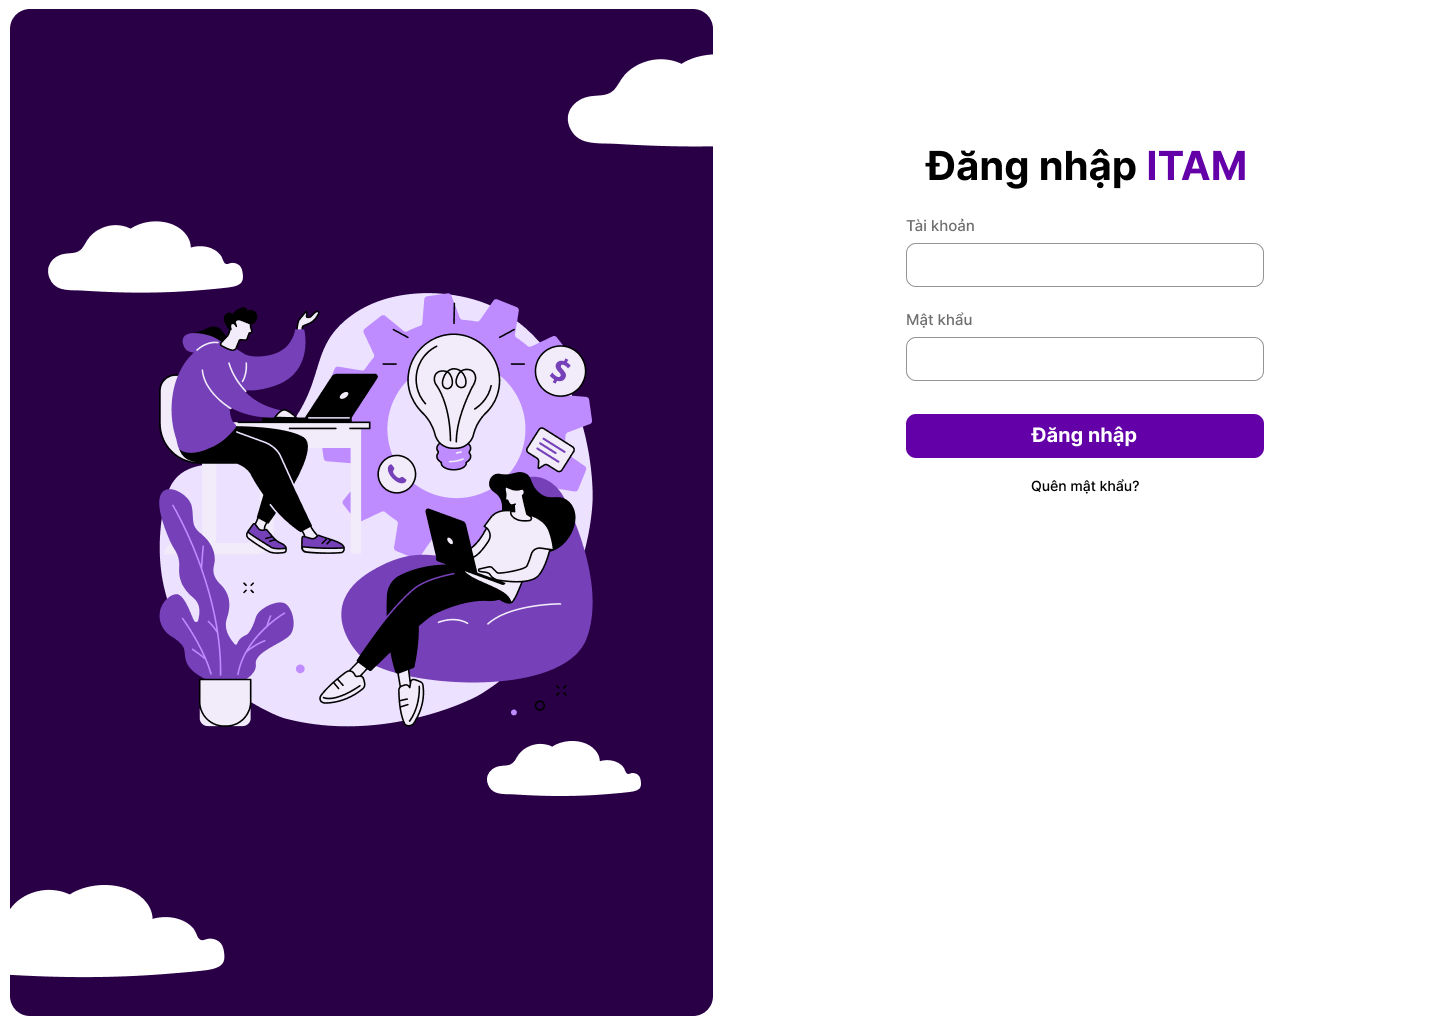
\includegraphics[width=14cm]{Images/C5/UI/Login.png}
%     \vspace{15pt}
%     \caption{Giao diện Đăng nhập}
% \end{figure}

\item{Bảng giám sát}\\
Bảng giám sát thời gian thực hiển thị trạng thái của máy tính có trong hệ thống, giúp nhân viên IT dễ dàng thực hiện giám sát máy tính, xử lý sự cố và cảnh báo một cách kịp thời, đảm bảo hoạt động của các máy tính trong hệ thống. Ngoài ra, tính năng xem tổng quan hoạt động của máy tính trong hệ thống giúp người dùng có cái nhìn tổng quan về hoạt động của các máy tính, cung cấp các thống kê về sự cố và tình trạng máy tính.
\begin{figure}[H]
    \centering
    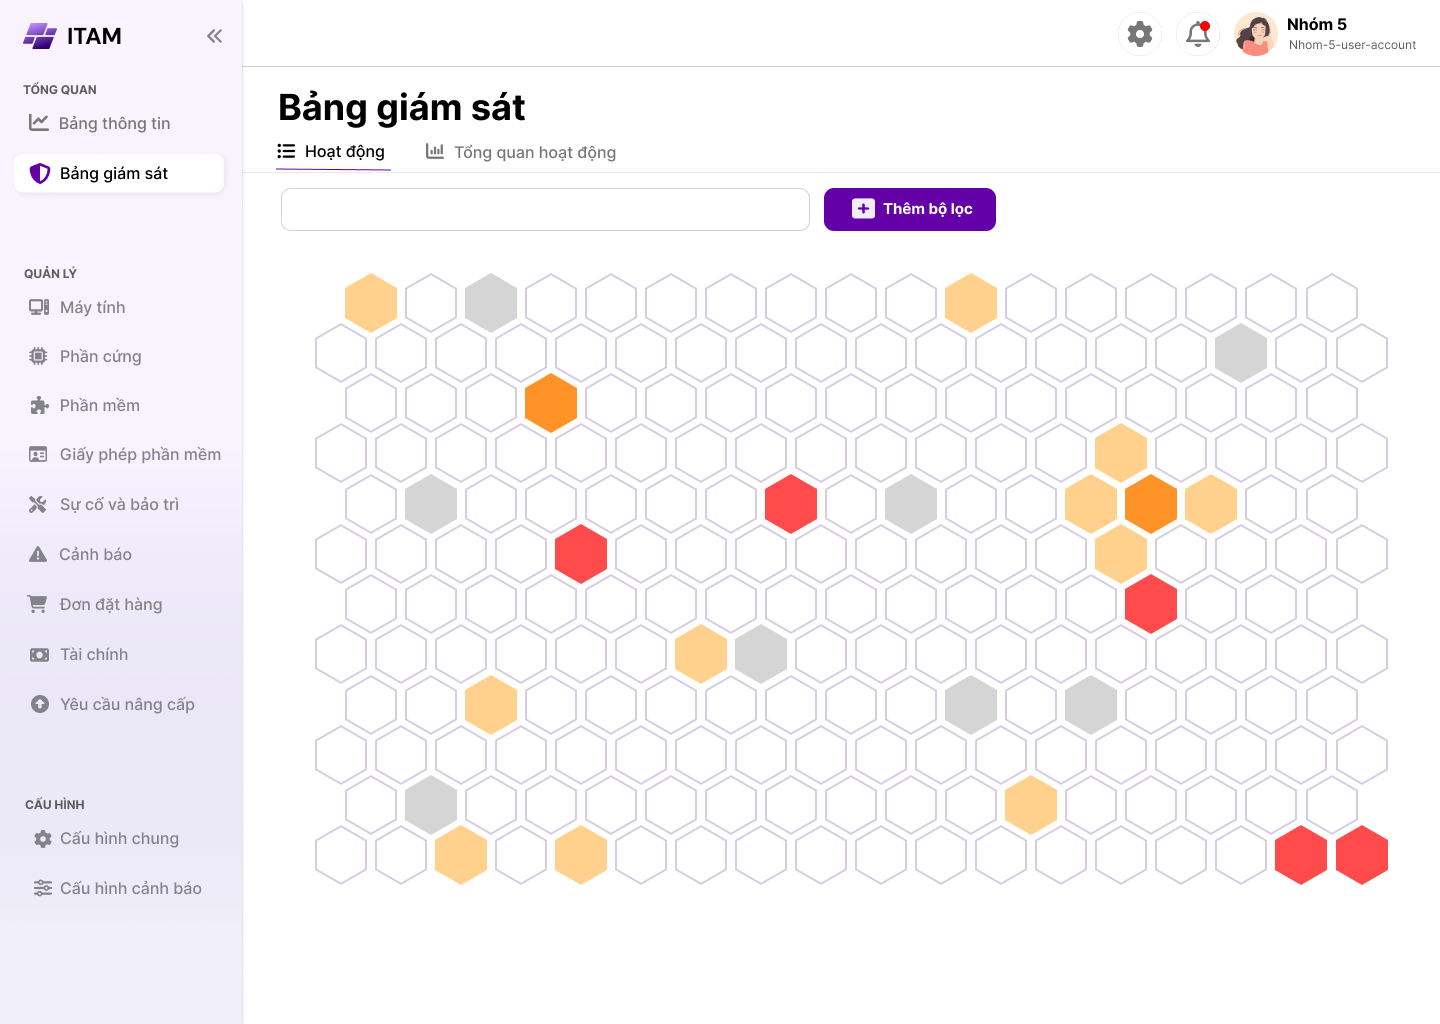
\includegraphics[width=14cm]{Images/C5/UI/Feature-Bảng giám sát 1.1.png}
    \vspace{15pt}
    \caption{Giao diện Bảng giám sát 1}
\end{figure}
% \begin{figure}[H]
%     \centering
%     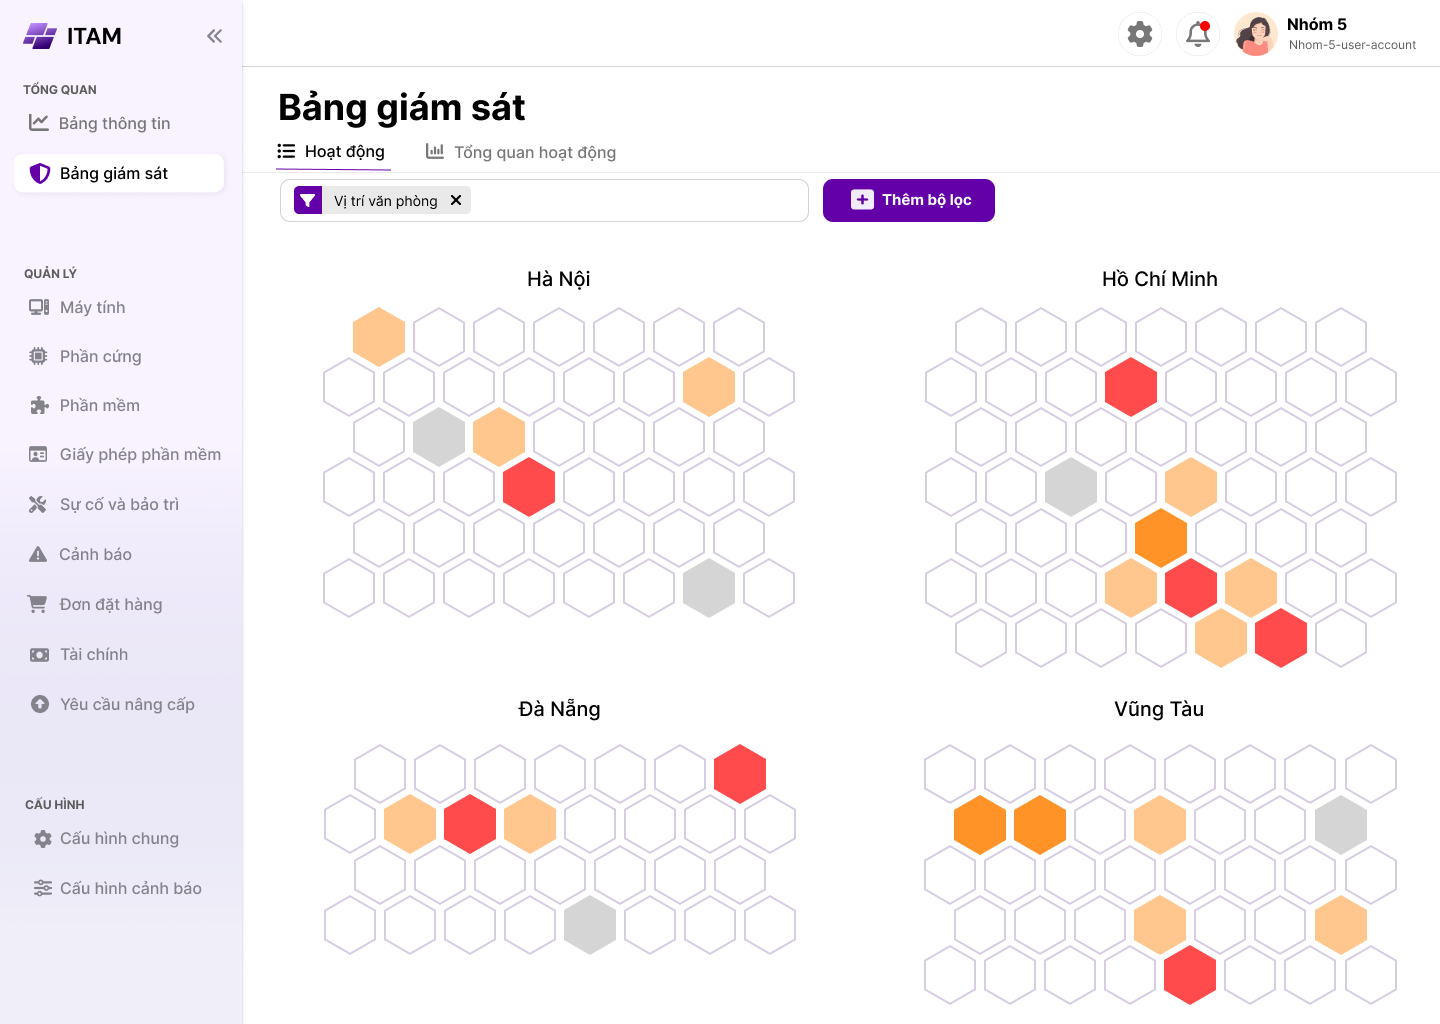
\includegraphics[width=14cm]{Images/C5/UI/Feature-Bảng giám sát 1.2.png}
%     \vspace{15pt}
%     \caption{Giao diện Bảng giám sát 2}
% \end{figure}
% \begin{figure}[H]
%     \centering
%     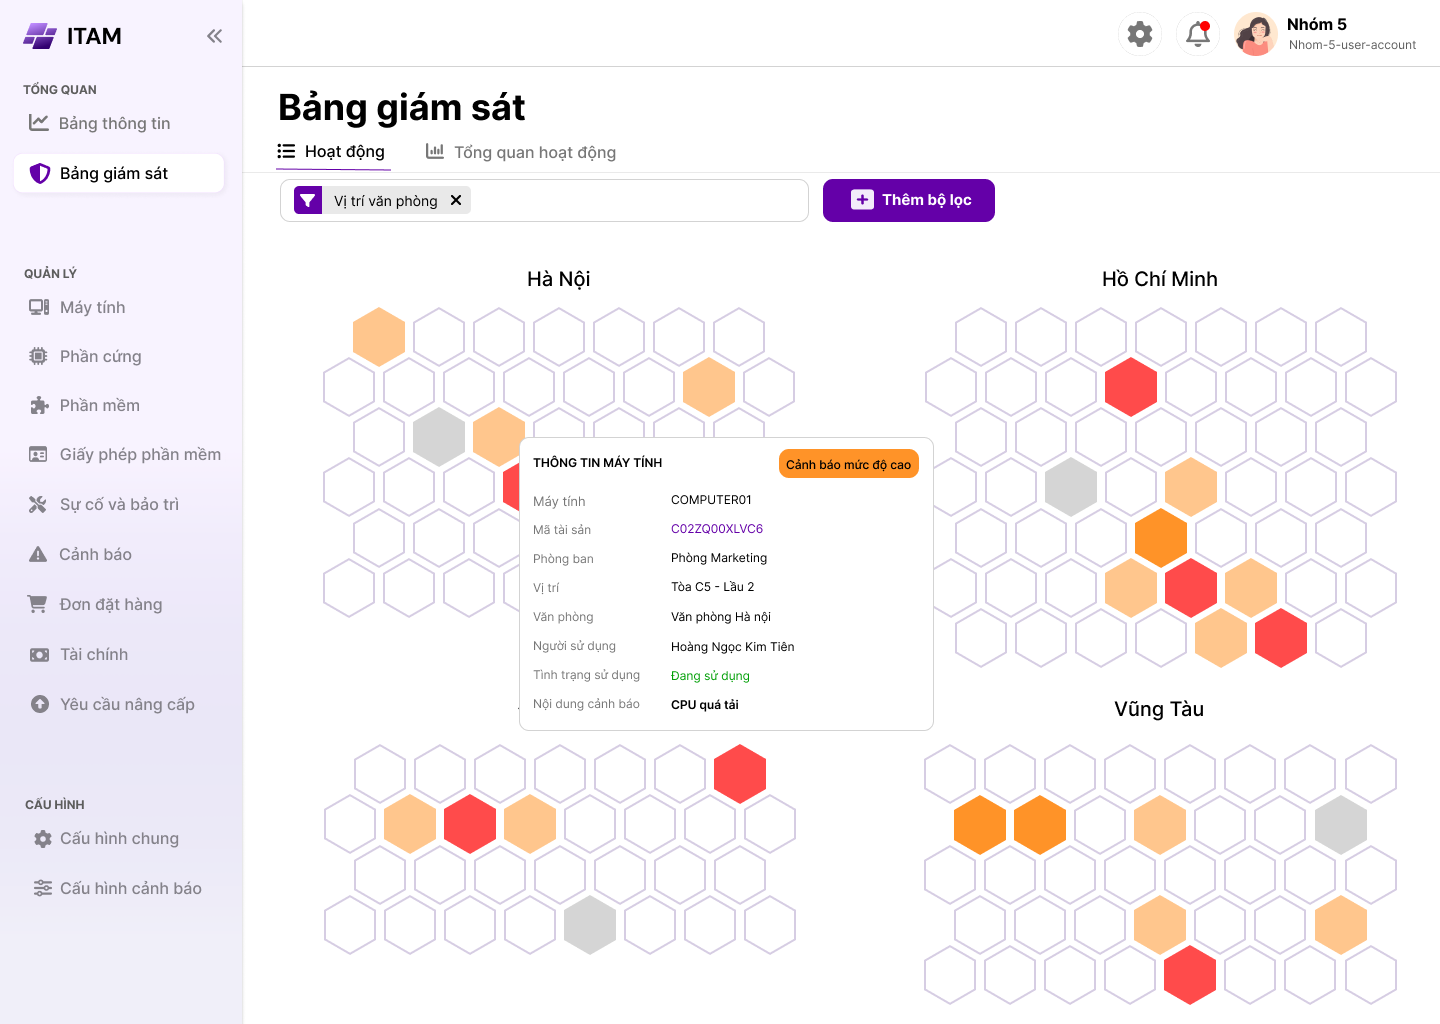
\includegraphics[width=14cm]{Images/C5/UI/Feature-Bảng giám sát 1.3.png}
%     \vspace{15pt}
%     \caption{Giao diện Bảng giám sát 2}
% \end{figure}
% \begin{figure}[H]
%     \centering
%     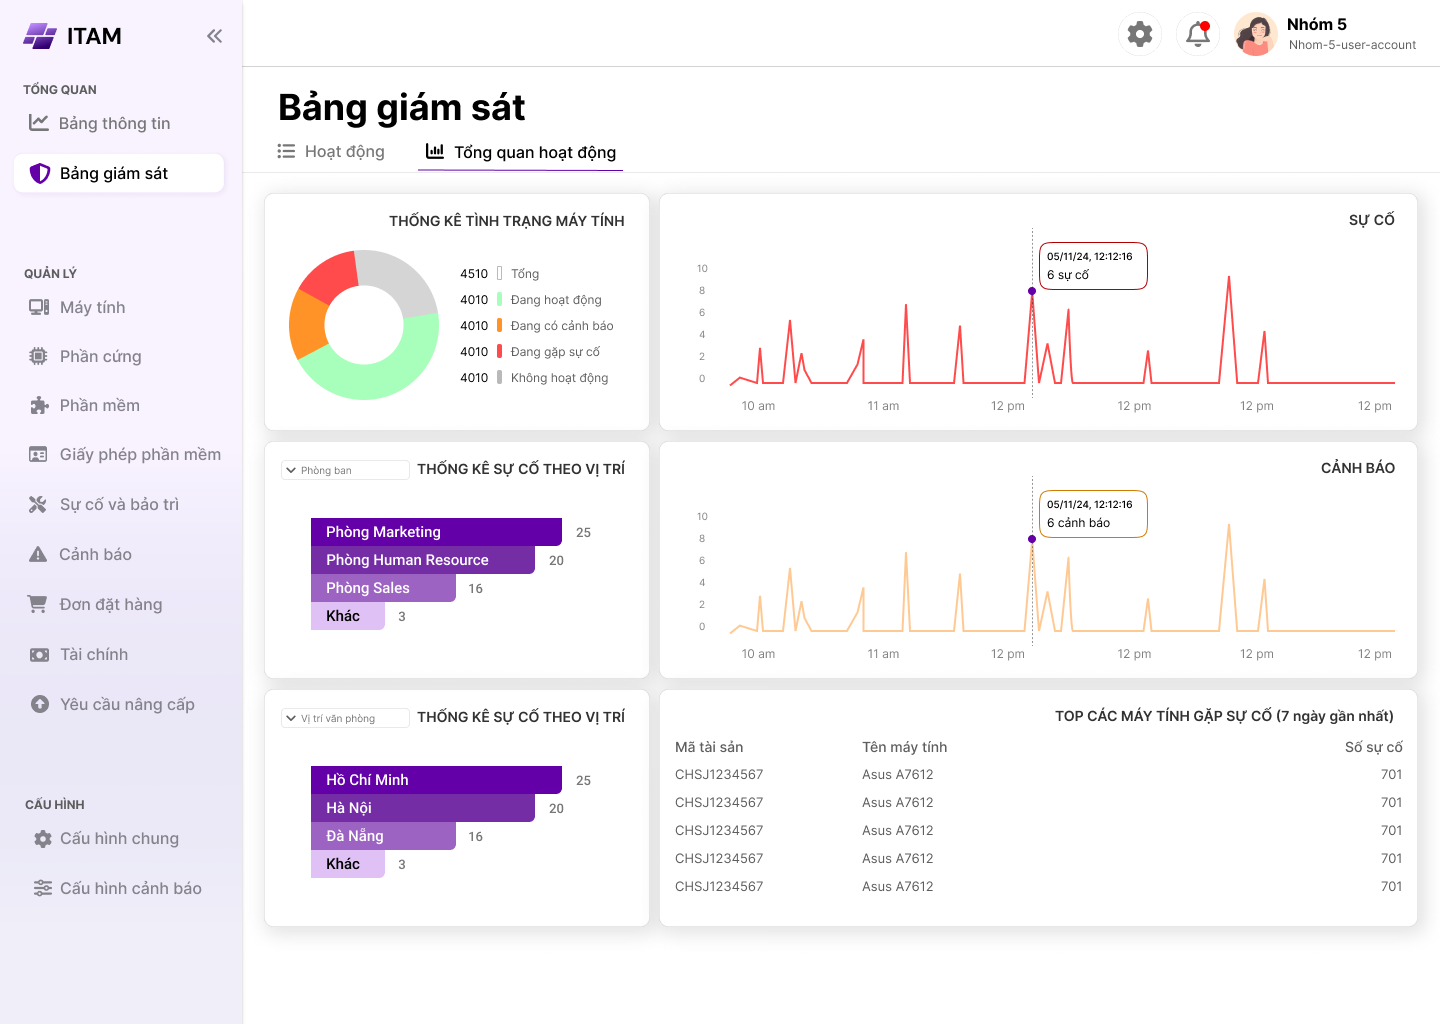
\includegraphics[width=14cm]{Images/C5/UI/Feature-Bảng giám sát 2.png}
%     \vspace{15pt}
%     \caption{Giao diện Bảng giám sát 3}
% \end{figure}

\item{Quản lý máy tính}\\
Quản lý máy tính cung cấp các tính năng cơ bản như xem danh sách máy tính, xem thông tin chi tiết máy tính, chỉnh sửa thông tin chi tiết máy tính, thêm máy tính, gửi yêu cầu nâng cấp, gửi yêu cầu bảo trì, và xem báo cáo tổng quan về máy tính trong hệ thống.\\
Thông tin chi tiết của máy tính gồm:
\begin{itemize}
    \item Thông tin chung như tên, số serial, loại máy tính, địa chỉ MAC,...
    \item Thông tin phần cứng của máy tính
    \item Thông tin phần mềm của máy tính
    \item Thông tin vòng đời của máy tính (Mua sắm, triển khai, sử dung, thanh lý)
    \item Hiệu suất sử dụng
\end{itemize}
% \begin{figure}[H]
%     \centering
%     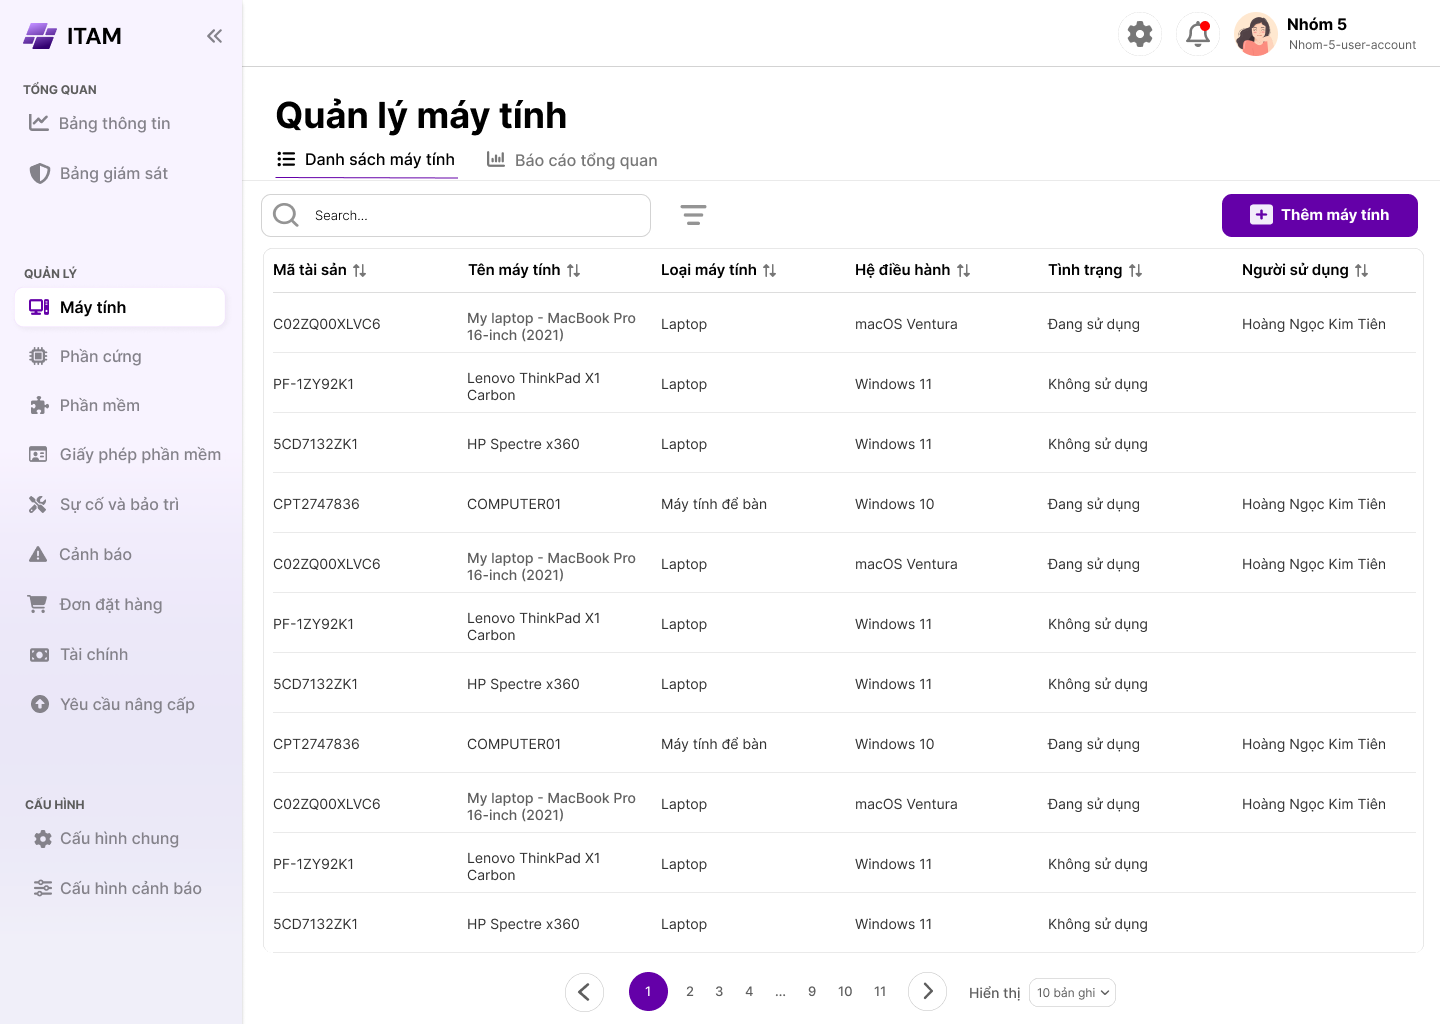
\includegraphics[width=14cm]{Images/C5/UI/Feature-Giám sát tài sản-Máy tính 1.1.png}
%     \vspace{15pt}
%     \caption{Giao diện Quản lý máy tính 1}
% \end{figure}
% \begin{figure}[H]
%     \centering
%     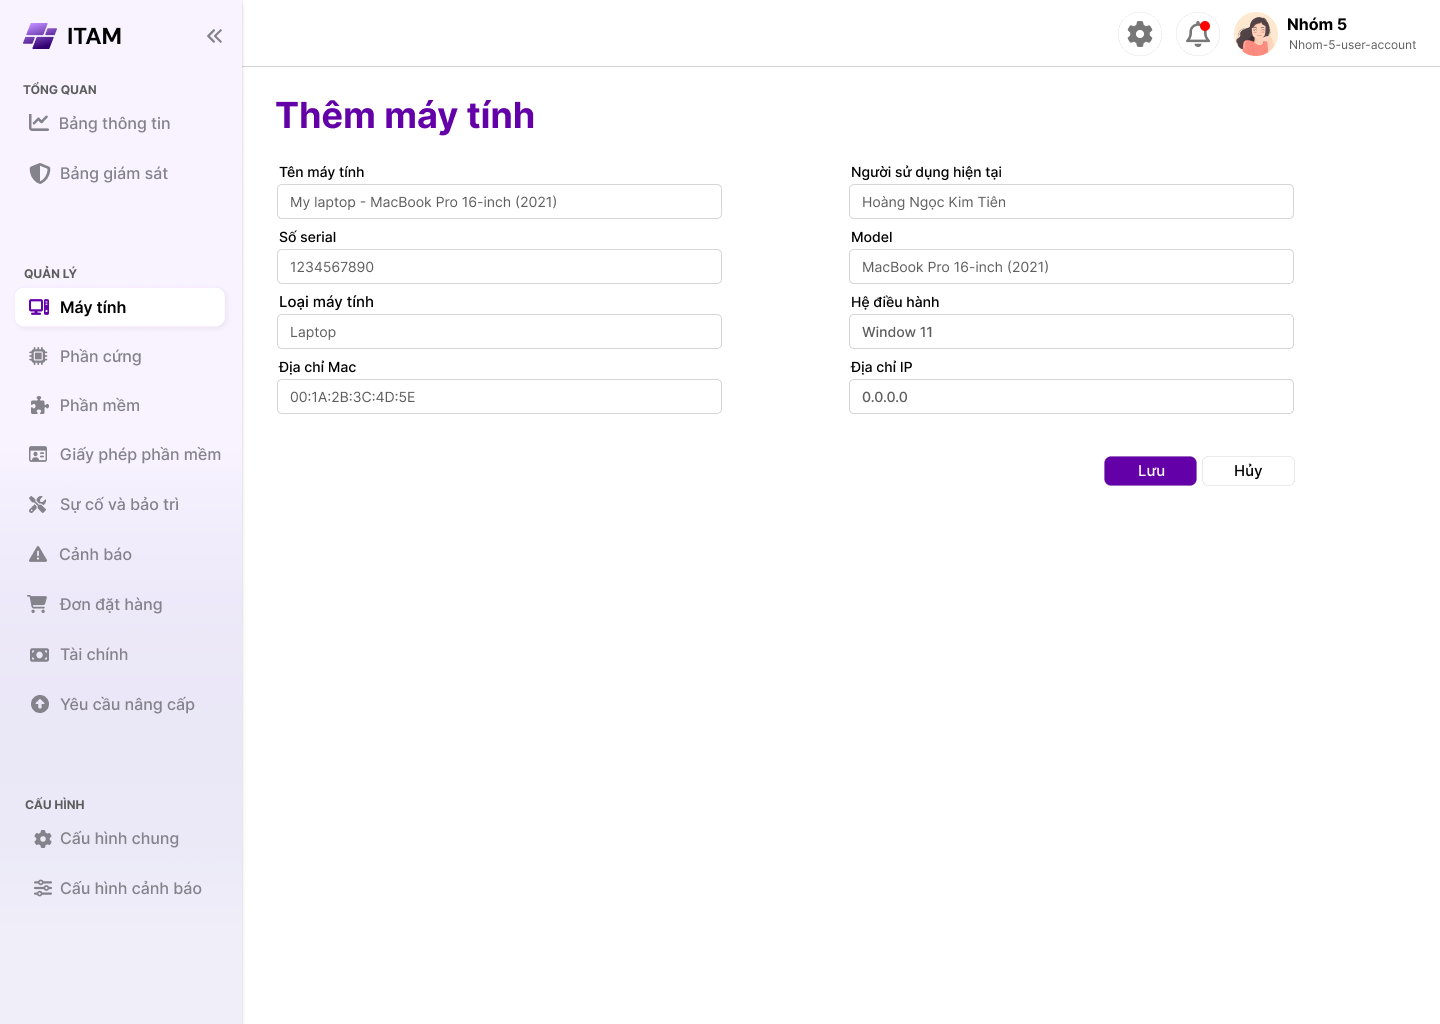
\includegraphics[width=14cm]{Images/C5/UI/Feature-Giám sát tài sản-Máy tính 1.2.png}
%     \vspace{15pt}
%     \caption{Giao diện Quản lý máy tính 2}
% \end{figure}
\begin{figure}[H]
    \centering
    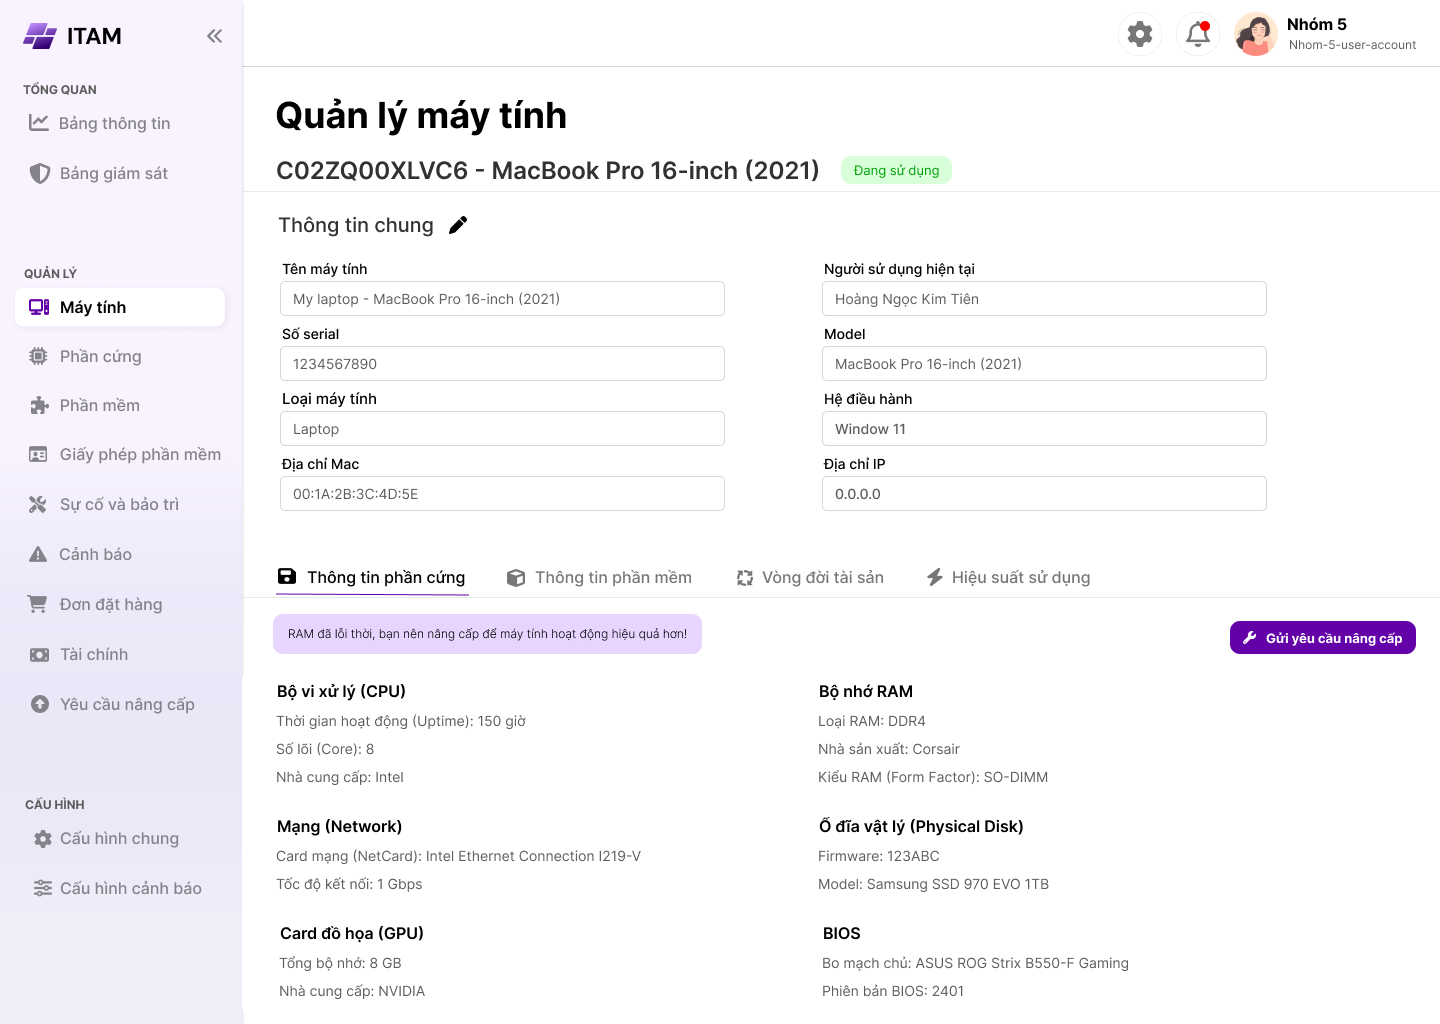
\includegraphics[width=14cm]{Images/C5/UI/Feature-Giám sát tài sản-Máy tính 2.1.png}
    \vspace{15pt}
    \caption{Giao diện Quản lý máy tính 1}
\end{figure}
% \begin{figure}[H]
%     \centering
%     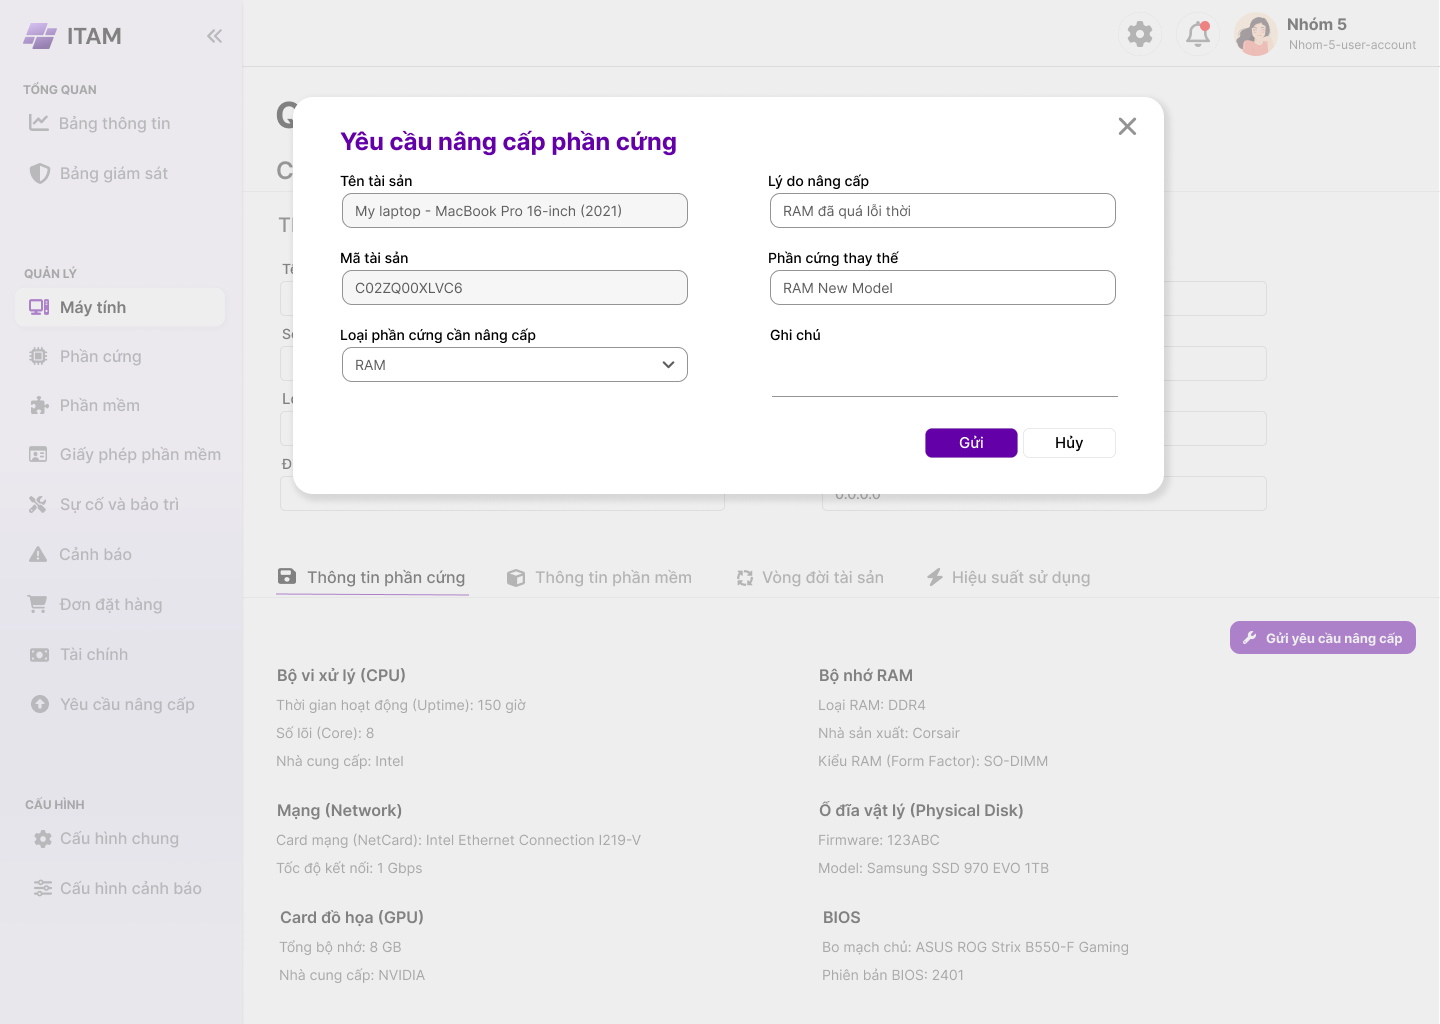
\includegraphics[width=14cm]{Images/C5/UI/Feature-Giám sát tài sản-Máy tính 2.2.png}
%     \vspace{15pt}
%     \caption{Giao diện Quản lý máy tính 4}
% \end{figure}
% \begin{figure}[H]
%     \centering
%     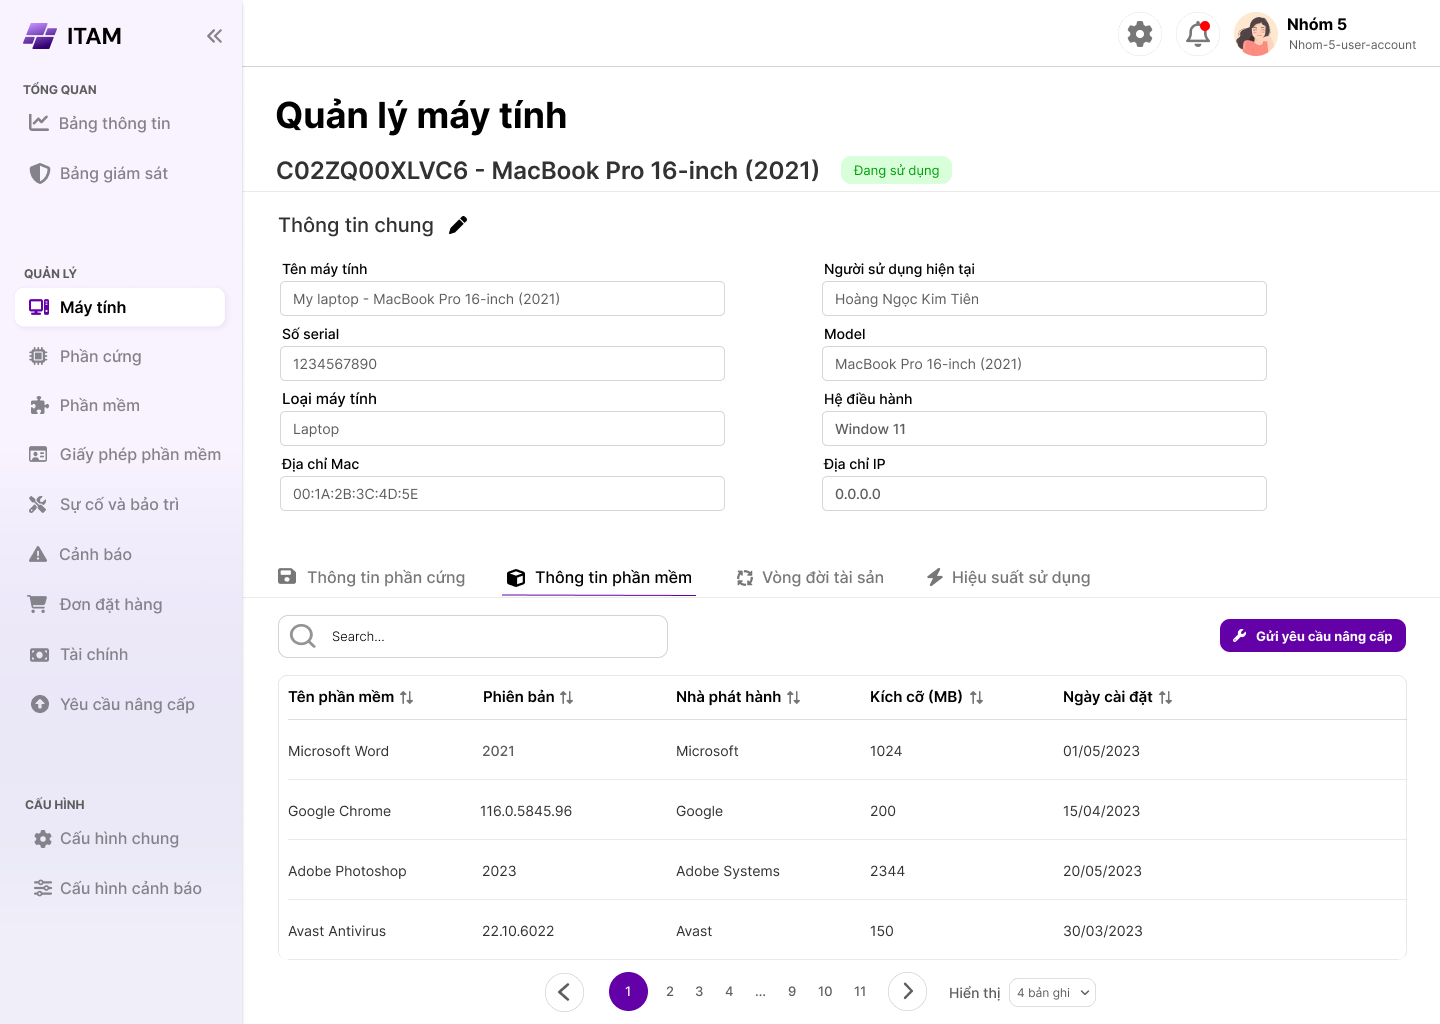
\includegraphics[width=14cm]{Images/C5/UI/Feature-Giám sát tài sản-Máy tính 3.1.png}
%     \vspace{15pt}
%     \caption{Giao diện Quản lý máy tính 5}
% \end{figure}
% \begin{figure}[H]
%     \centering
%     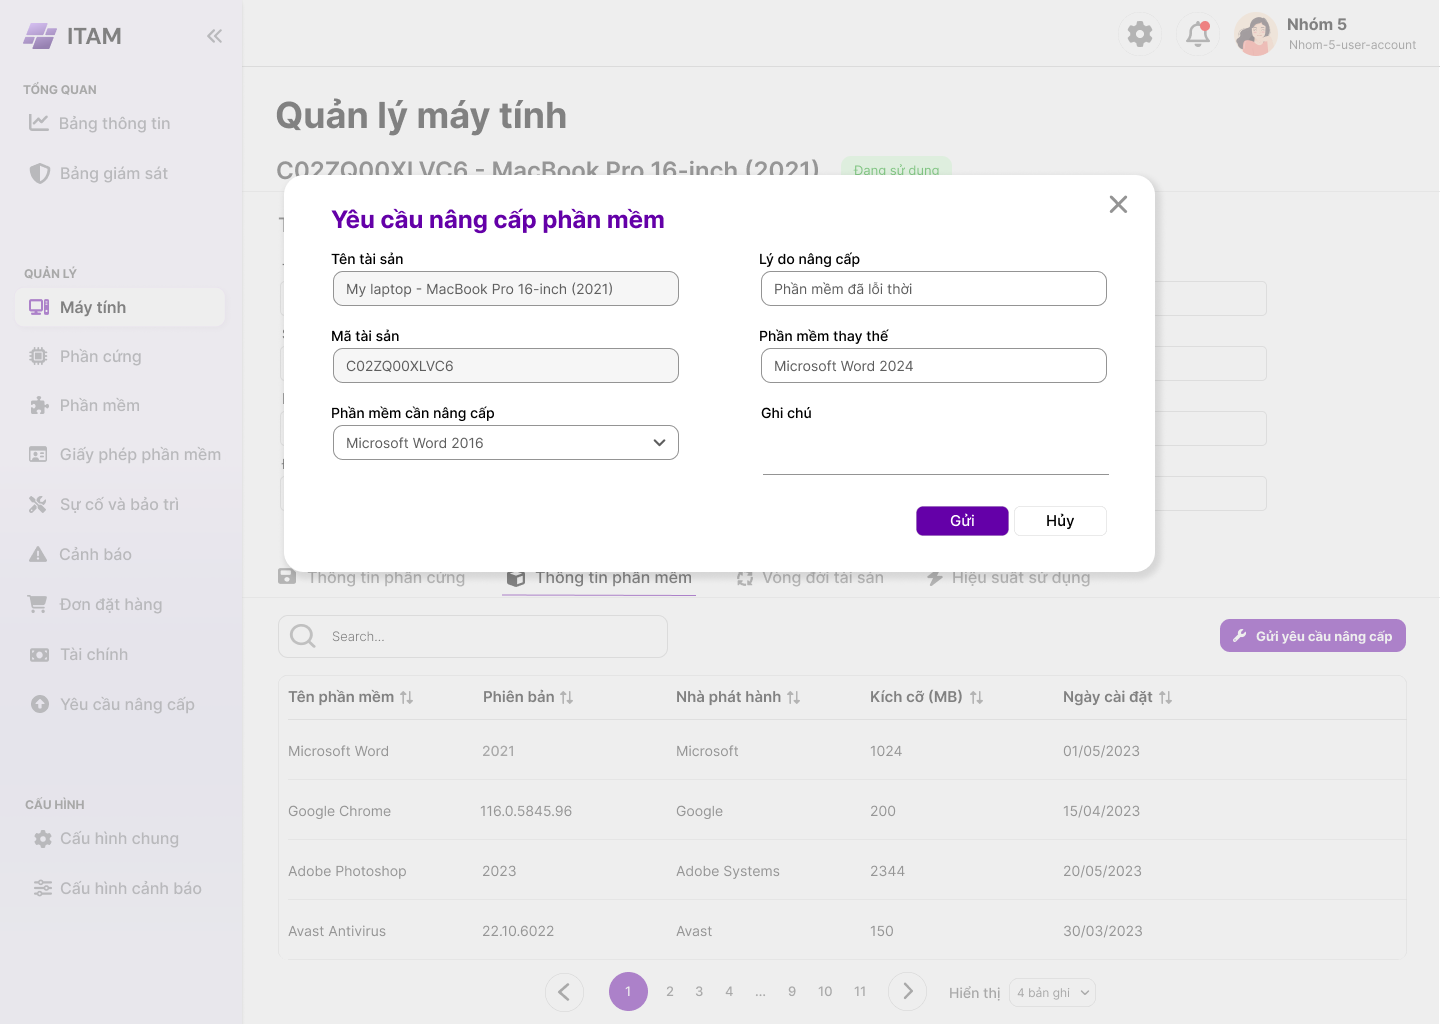
\includegraphics[width=14cm]{Images/C5/UI/Feature-Giám sát tài sản-Máy tính 3.2.png}
%     \vspace{15pt}
%     \caption{Giao diện Quản lý máy tính 6}
% \end{figure}
% \begin{figure}[H]
%     \centering
%     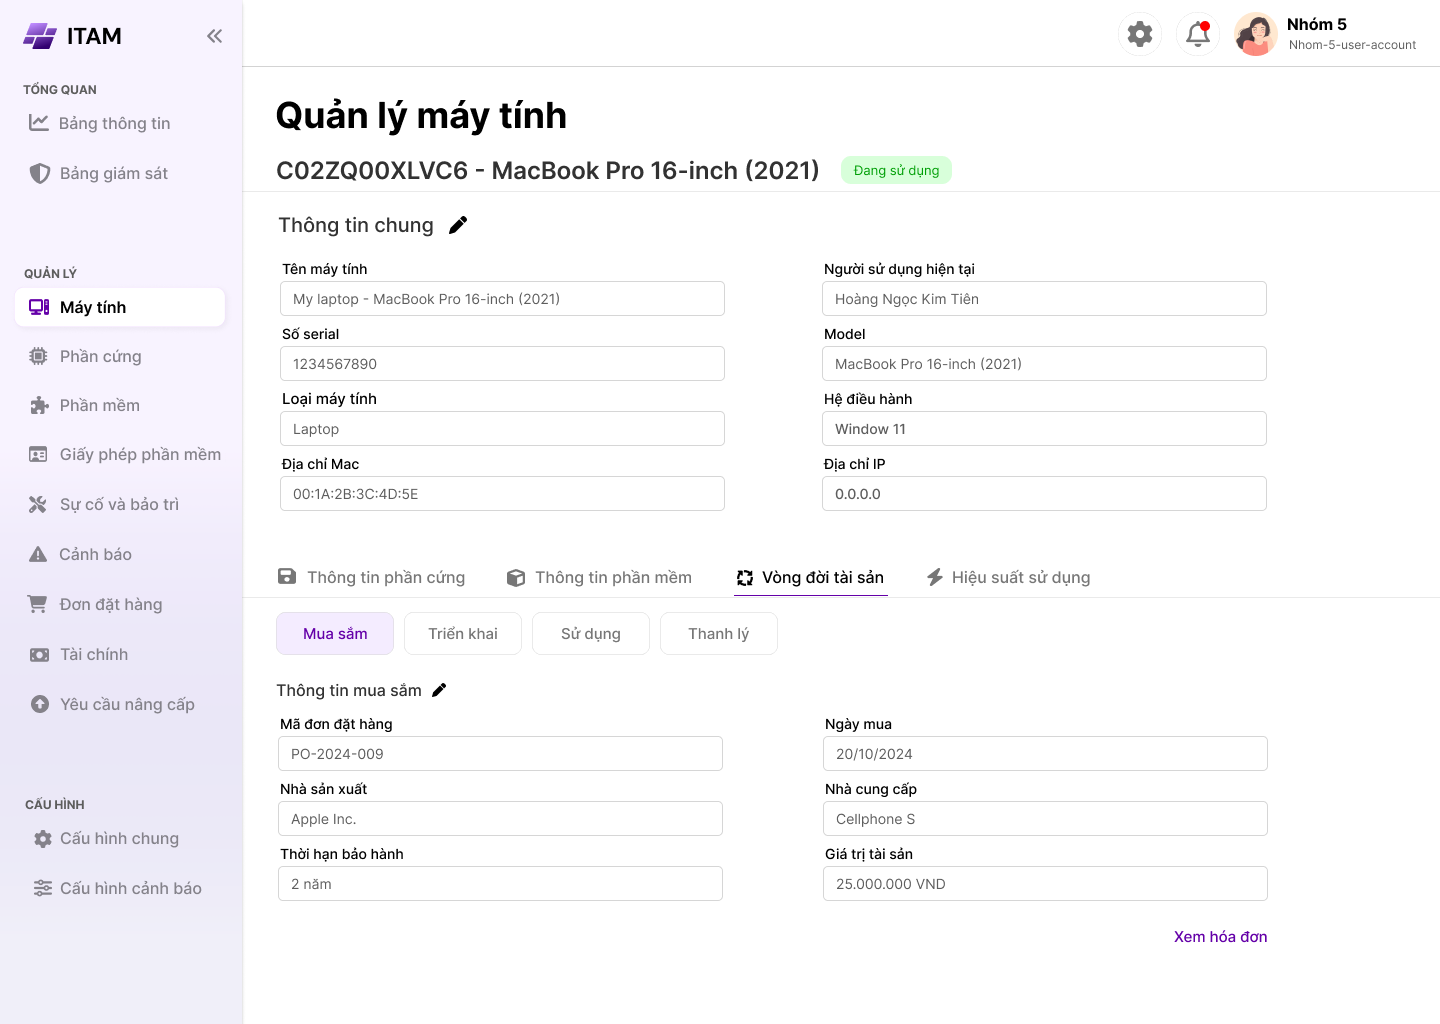
\includegraphics[width=14cm]{Images/C5/UI/Feature-Giám sát tài sản-Máy tính 4.1.png}
%     \vspace{15pt}
%     \caption{Giao diện Quản lý máy tính 7}
% \end{figure}
% \begin{figure}[H]
%     \centering
%     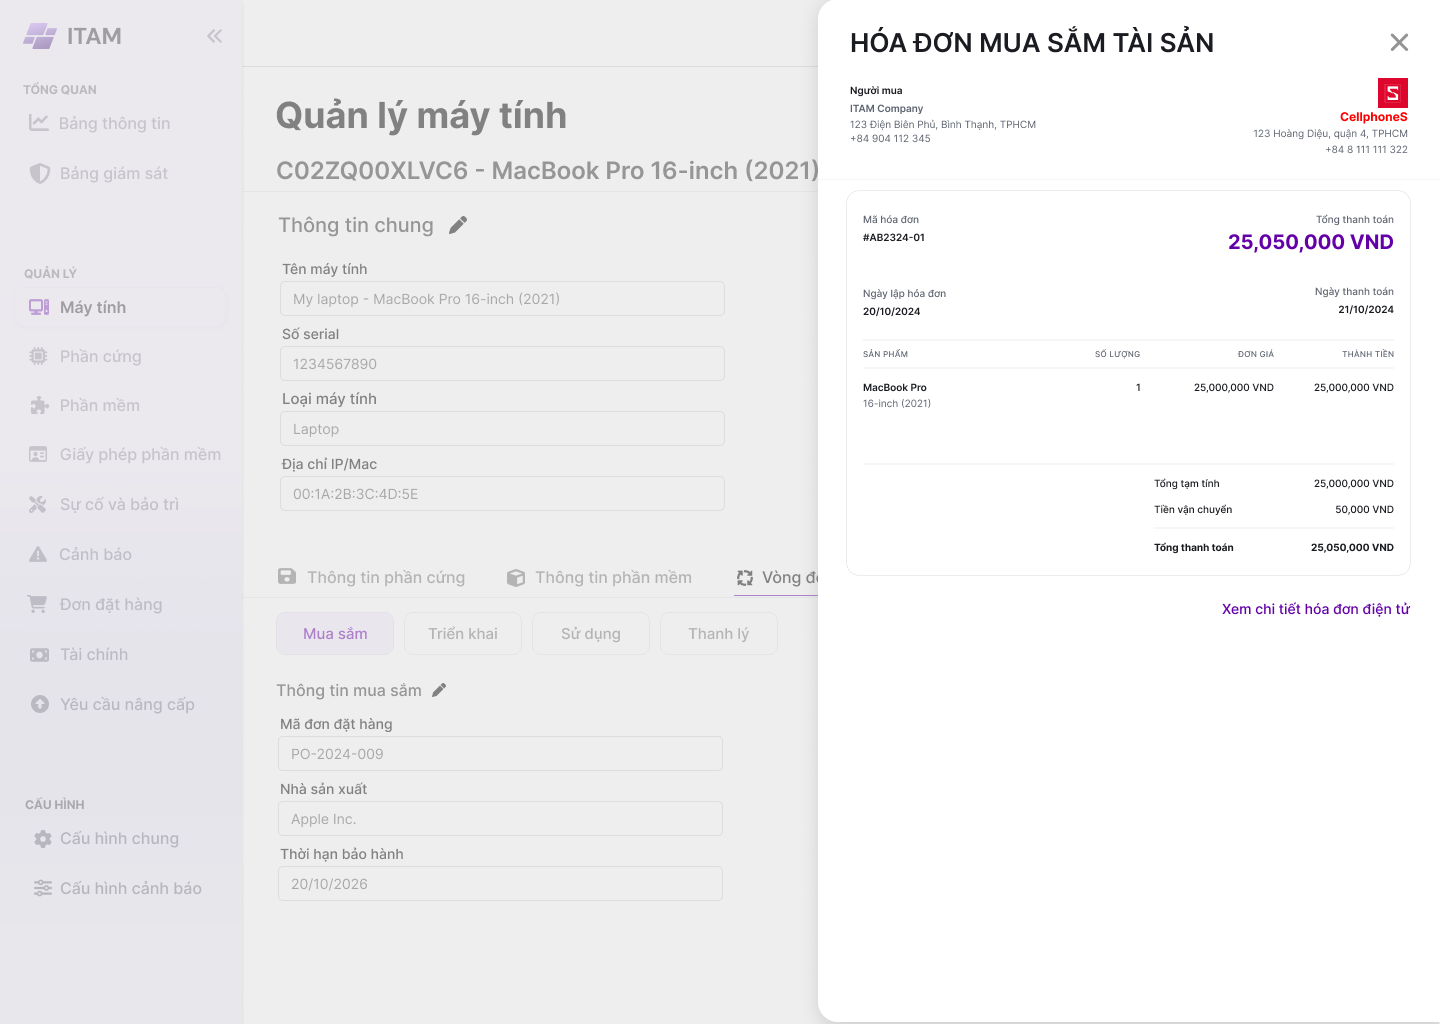
\includegraphics[width=14cm]{Images/C5/UI/Feature-Giám sát tài sản-Máy tính 4.2.png}
%     \vspace{15pt}
%     \caption{Giao diện Quản lý máy tính 8}
% \end{figure}
% \begin{figure}[H]
%     \centering
%     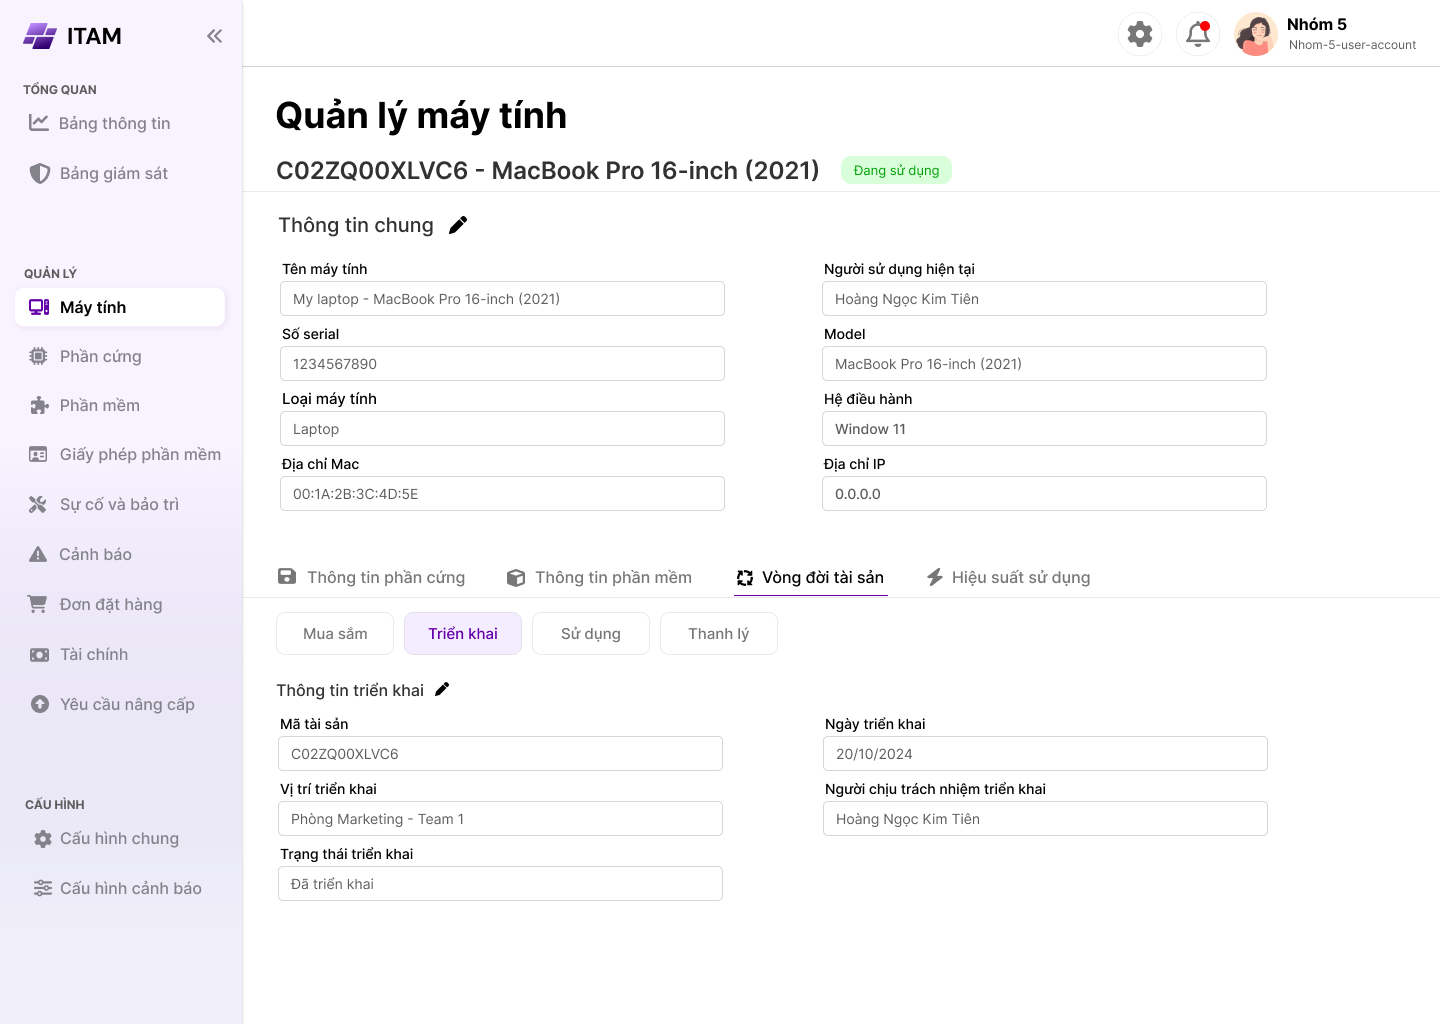
\includegraphics[width=14cm]{Images/C5/UI/Feature-Giám sát tài sản-Máy tính 5.png}
%     \vspace{15pt}
%     \caption{Giao diện Quản lý máy tính 8}
% \end{figure}
% \begin{figure}[H]
%     \centering
%     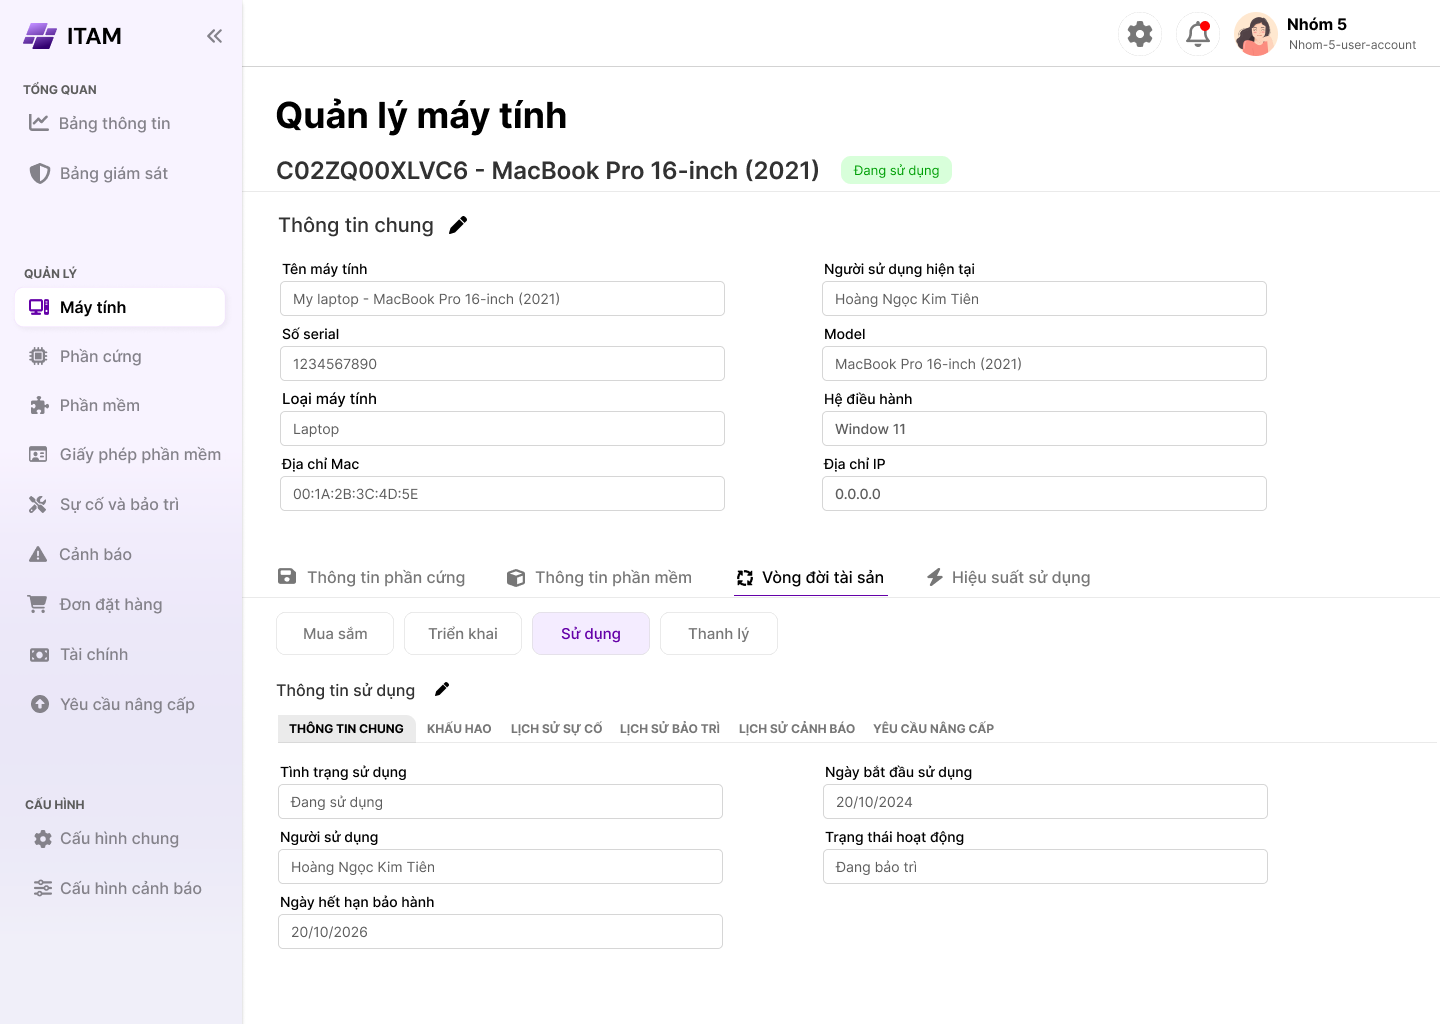
\includegraphics[width=14cm]{Images/C5/UI/Feature-Giám sát tài sản-Máy tính 6.1.png}
%     \vspace{15pt}
%     \caption{Giao diện Quản lý máy tính 9}
% \end{figure}
% \begin{figure}[H]
%     \centering
%     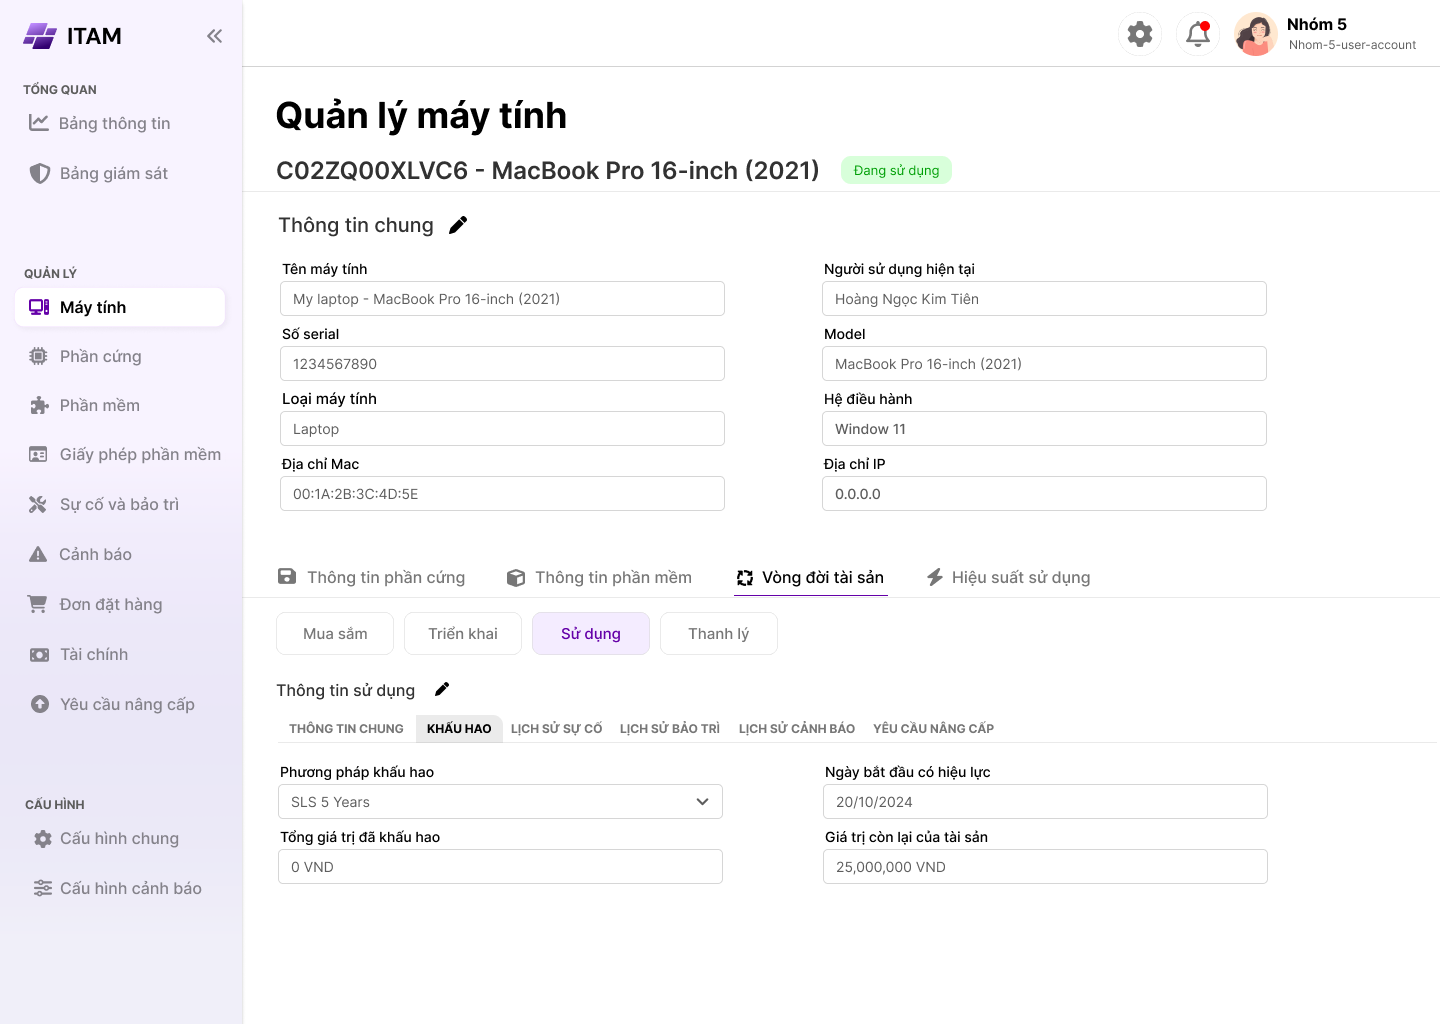
\includegraphics[width=14cm]{Images/C5/UI/Feature-Giám sát tài sản-Máy tính 6.2.png}
%     \vspace{15pt}
%     \caption{Giao diện Quản lý máy tính 11}
% \end{figure}
% \begin{figure}[H]
%     \centering
%     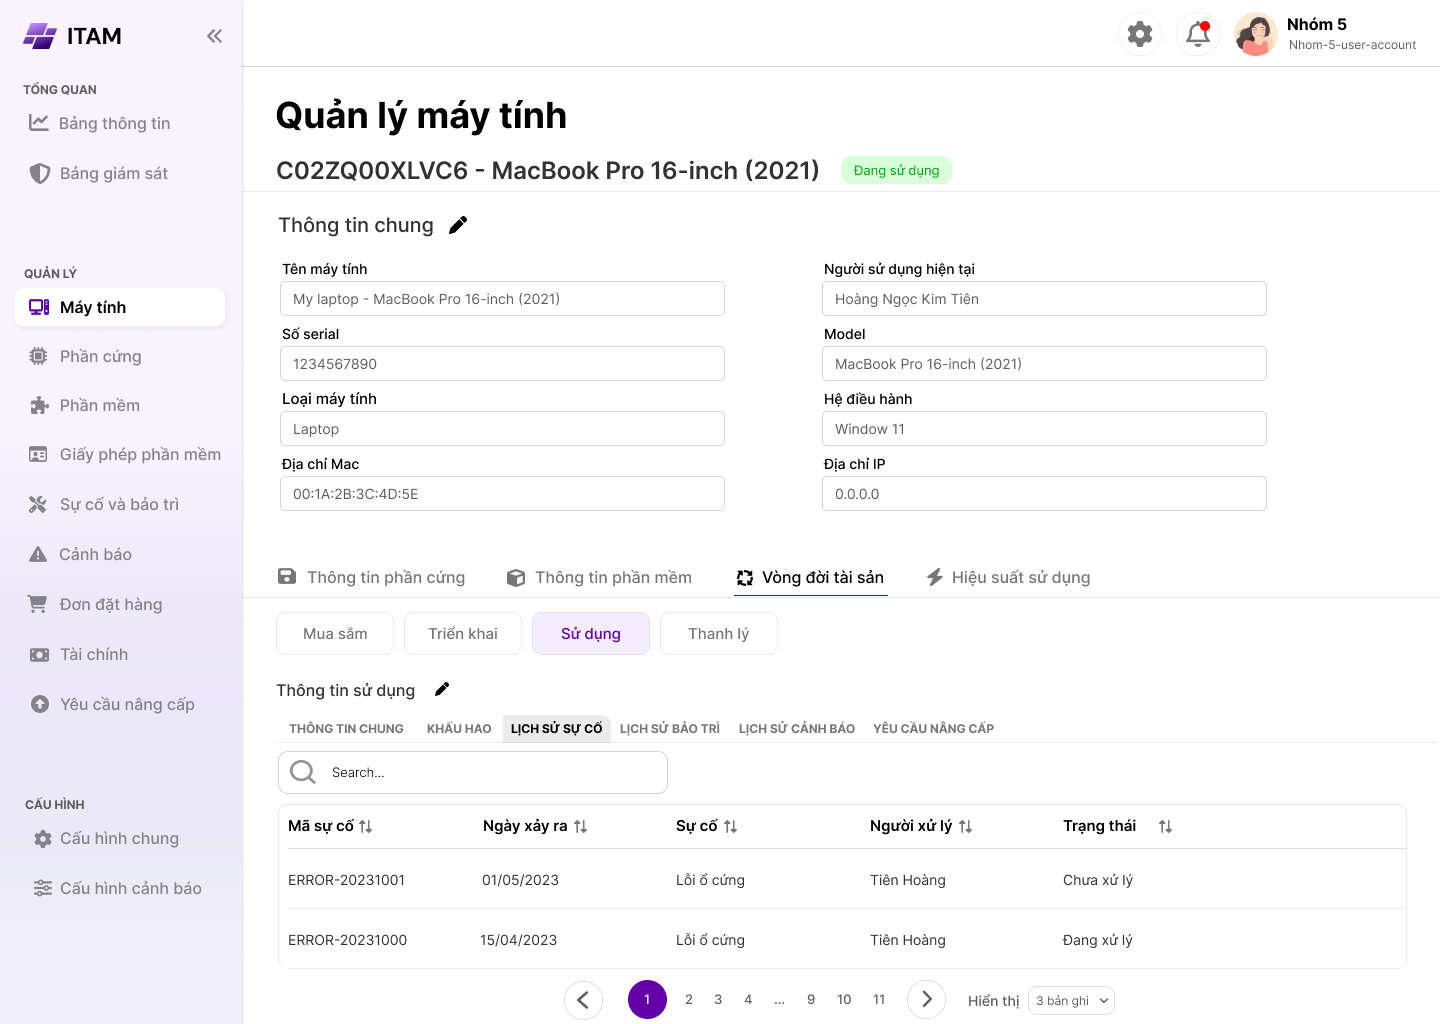
\includegraphics[width=14cm]{Images/C5/UI/Feature-Giám sát tài sản-Máy tính 6.3.png}
%     \vspace{15pt}
%     \caption{Giao diện Quản lý máy tính 12}
% \end{figure}
% \begin{figure}[H]
%     \centering
%     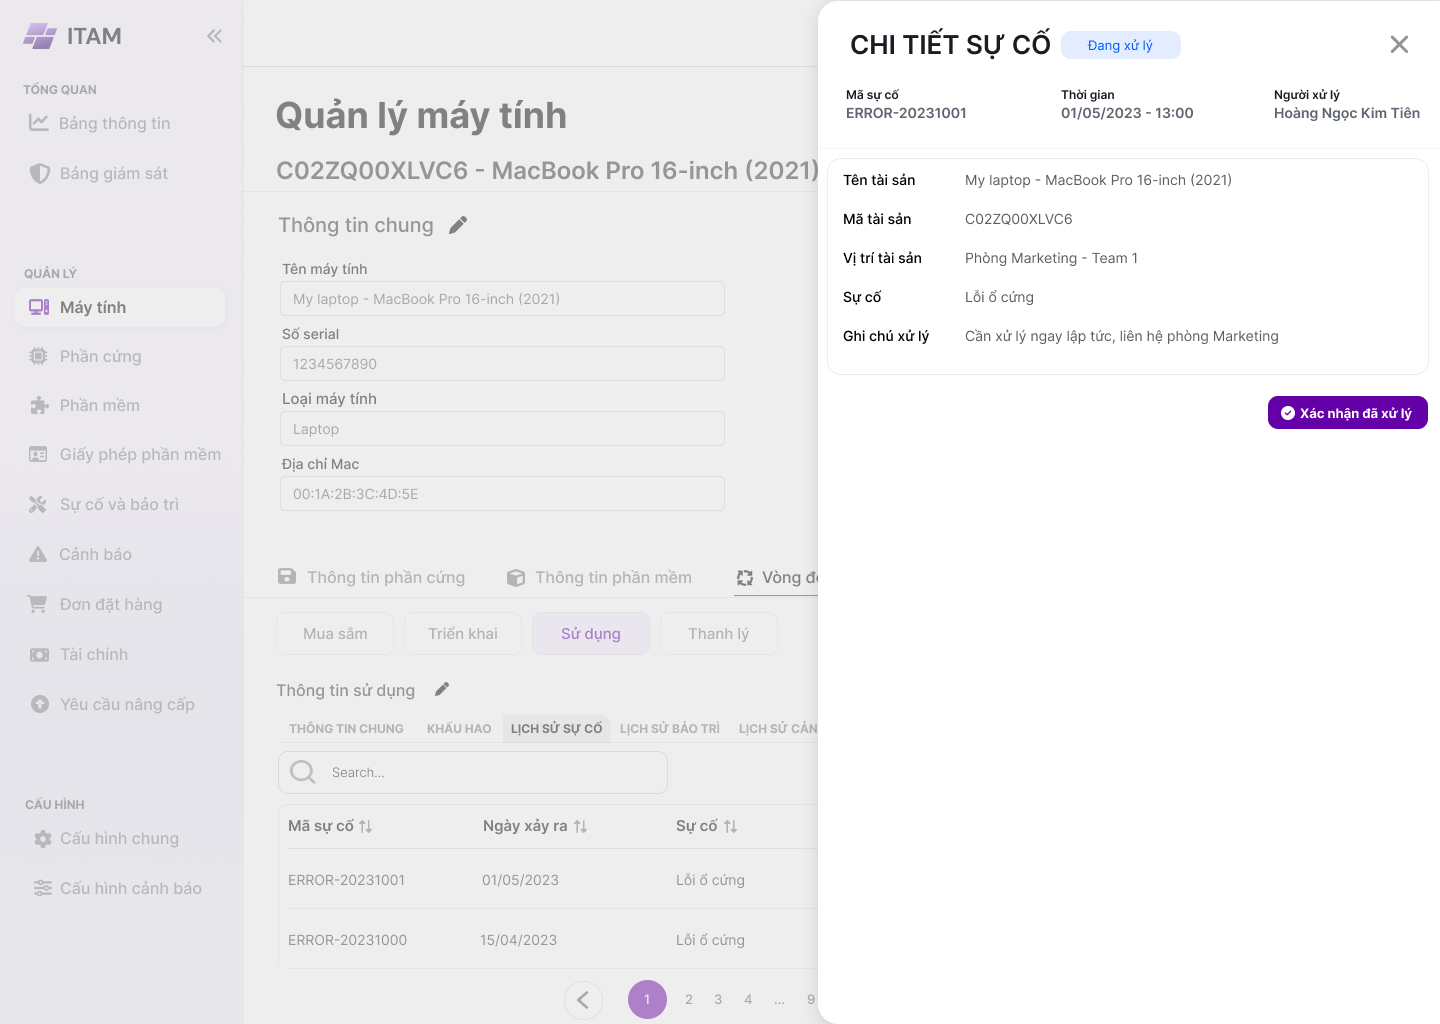
\includegraphics[width=14cm]{Images/C5/UI/Feature-Giám sát tài sản-Máy tính 6.4.png}
%     \vspace{15pt}
%     \caption{Giao diện Quản lý máy tính 13}
% \end{figure}
% \begin{figure}[H]
%     \centering
%     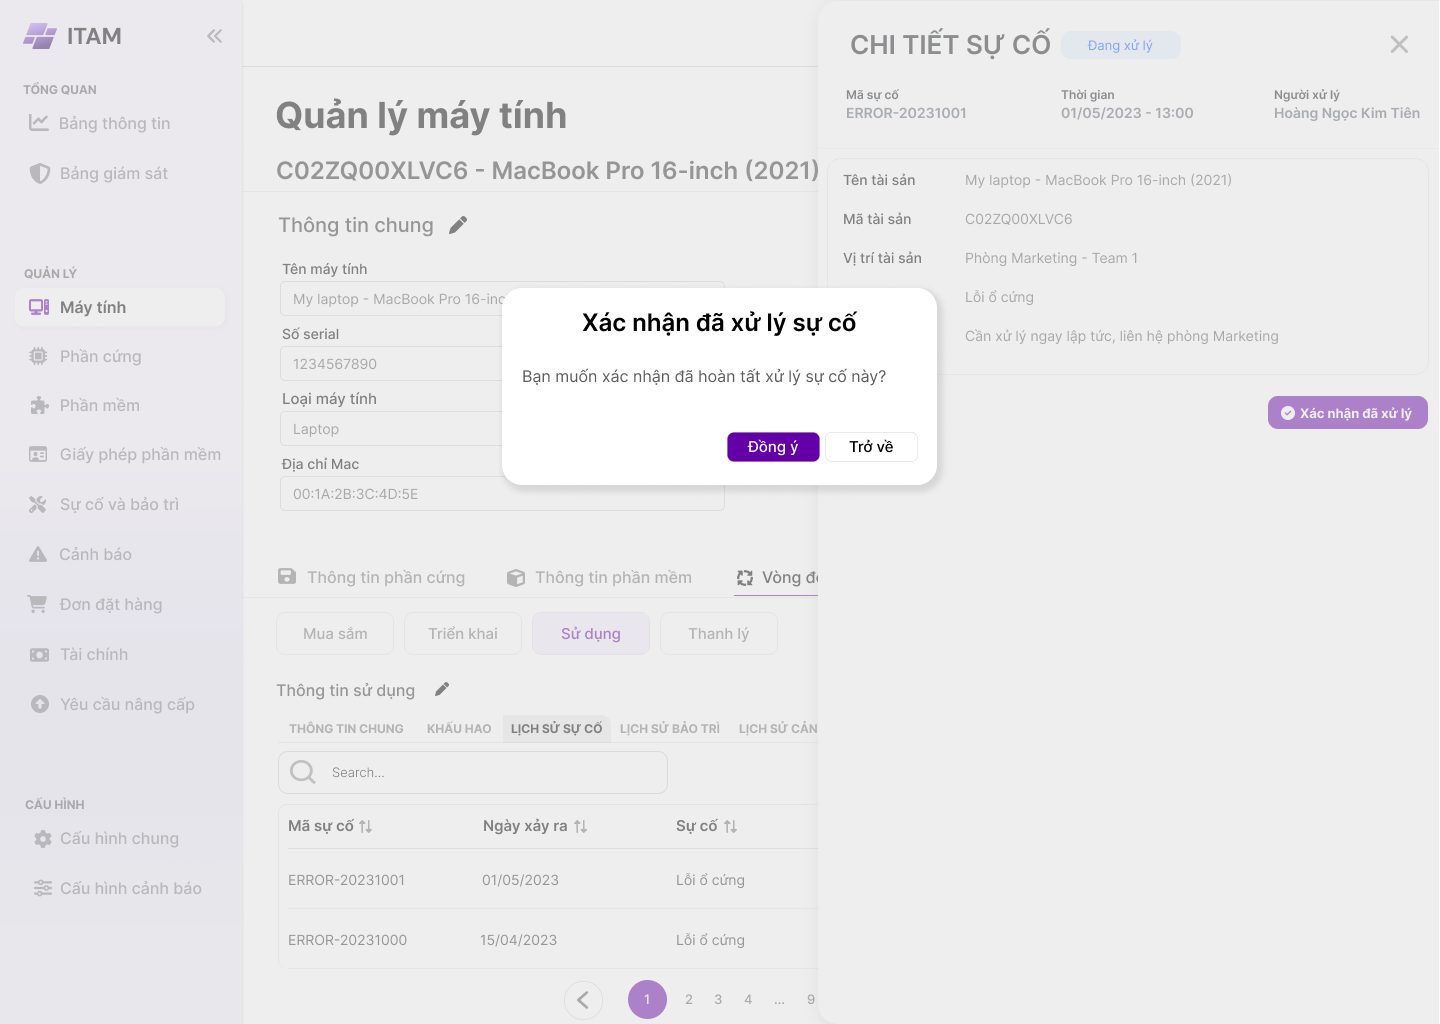
\includegraphics[width=14cm]{Images/C5/UI/Feature-Giám sát tài sản-Máy tính 6.5.png}
%     \vspace{15pt}
%     \caption{Giao diện Quản lý máy tính 14}
% \end{figure}
% \begin{figure}[H]
%     \centering
%     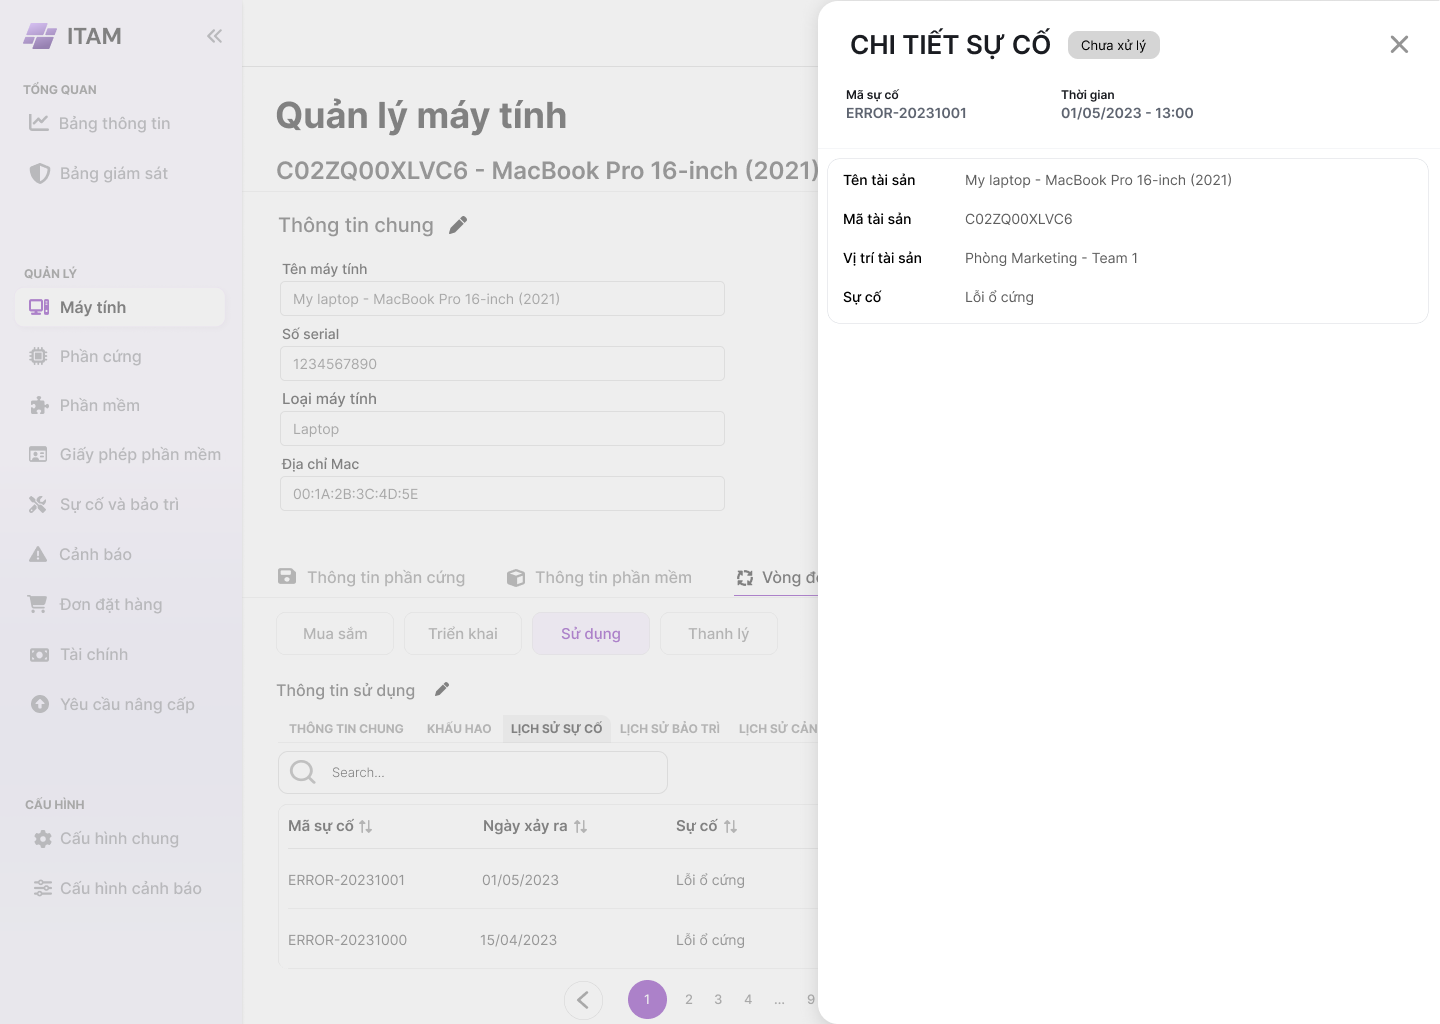
\includegraphics[width=14cm]{Images/C5/UI/Feature-Giám sát tài sản-Máy tính 6.6.png}
%     \vspace{15pt}
%     \caption{Giao diện Quản lý máy tính 15}
% \end{figure}
% \begin{figure}[H]
%     \centering
%     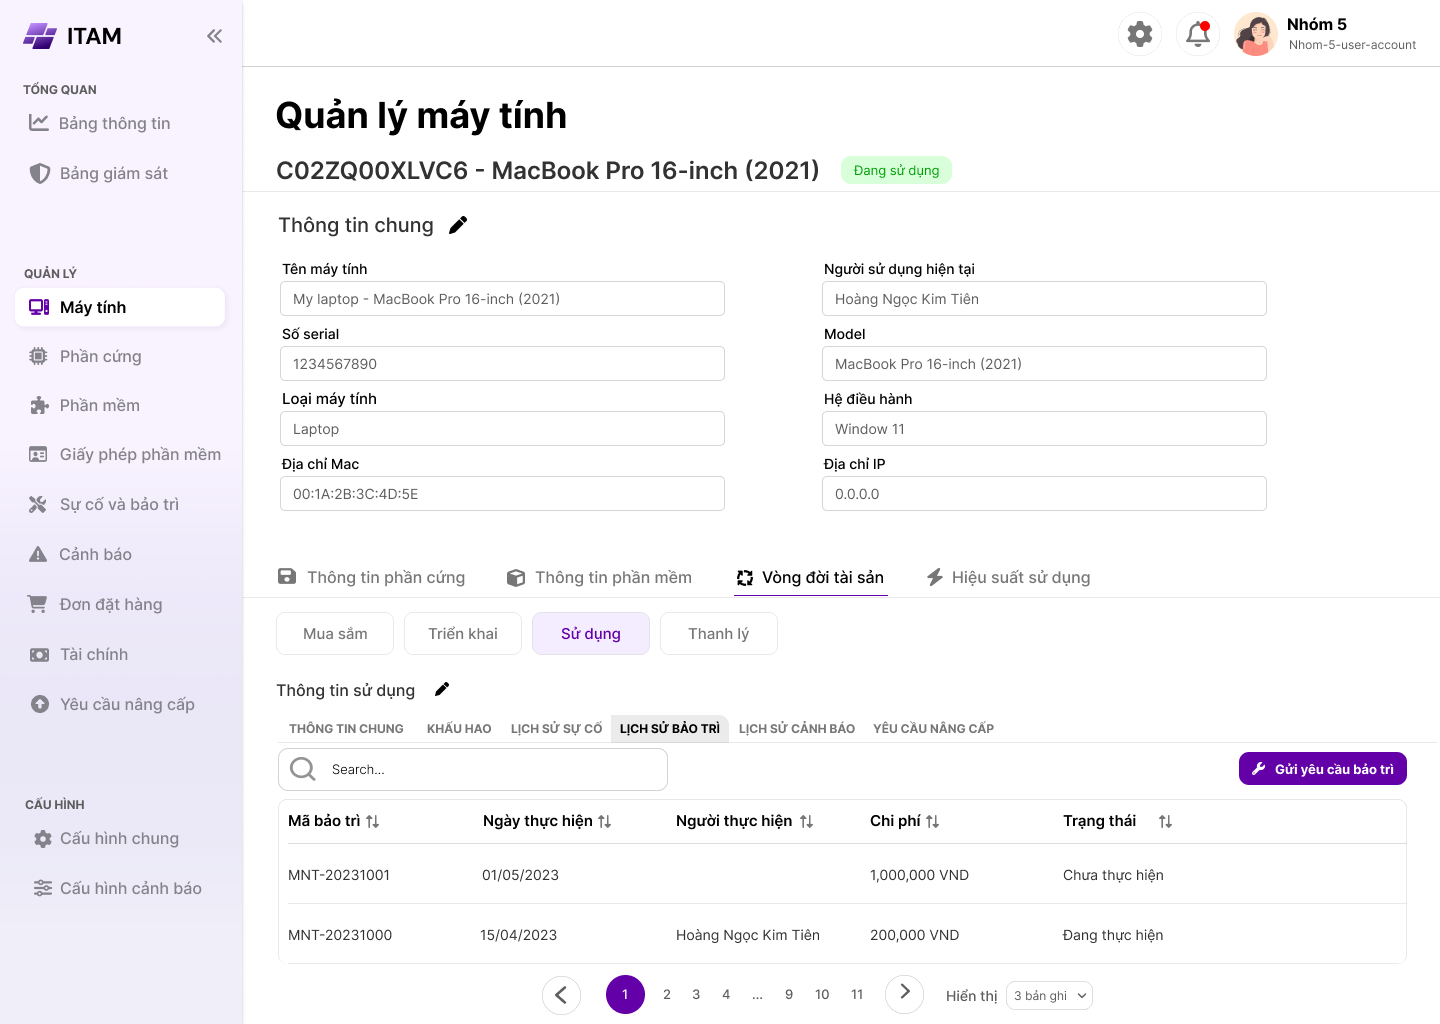
\includegraphics[width=14cm]{Images/C5/UI/Feature-Giám sát tài sản-Máy tính 6.8.png}
%     \vspace{15pt}
%     \caption{Giao diện Quản lý máy tính 10}
% \end{figure}
% \begin{figure}[H]
%     \centering
%     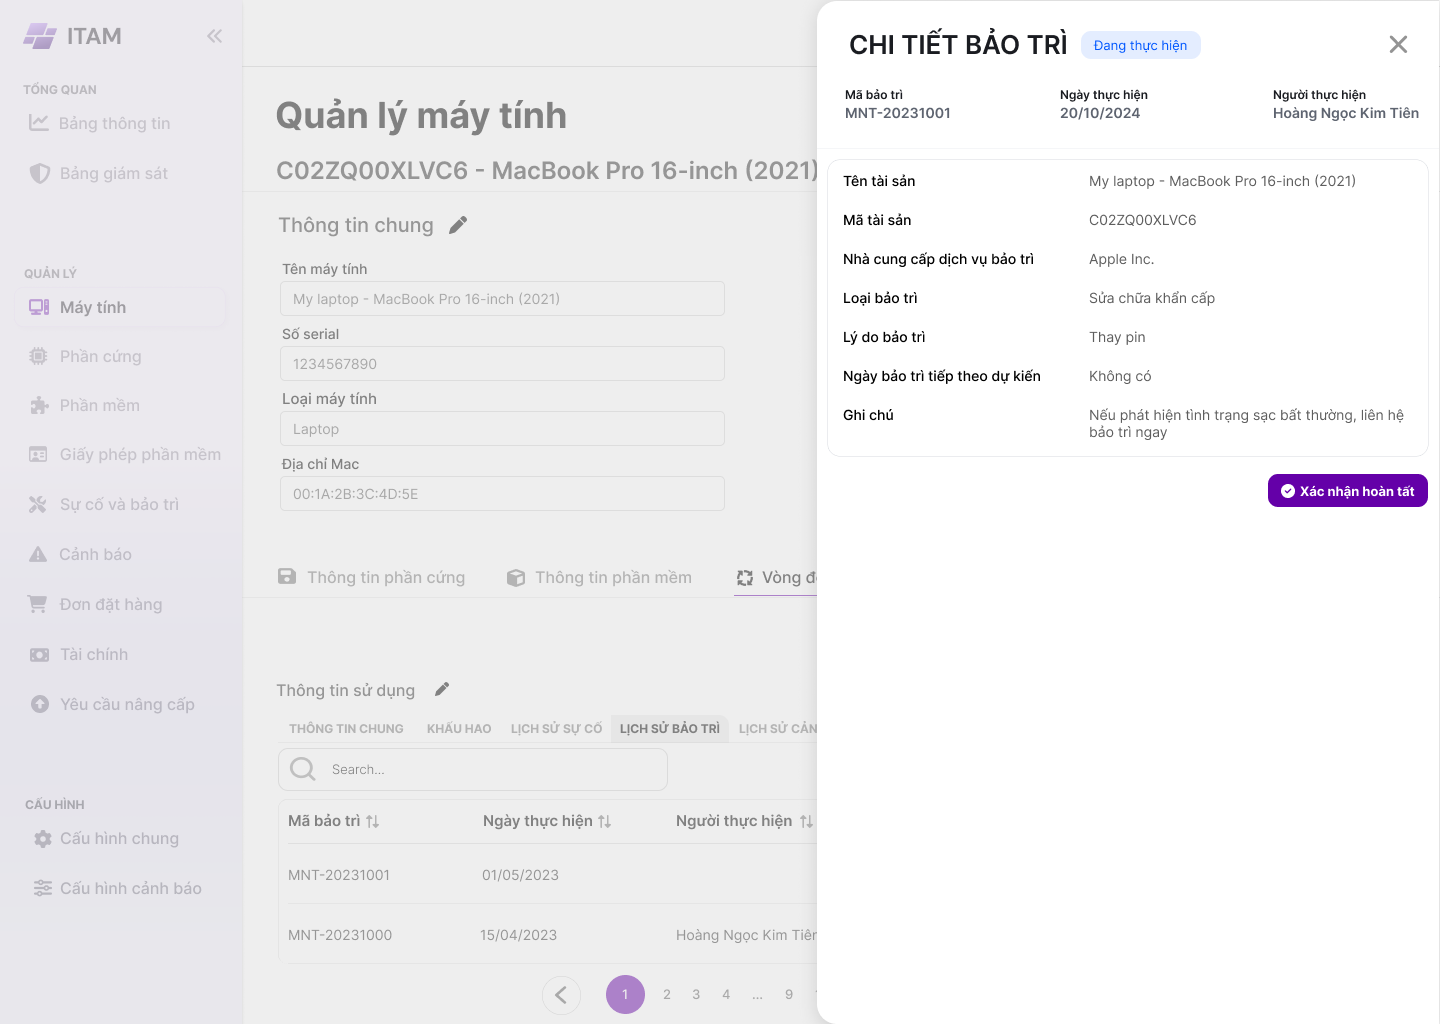
\includegraphics[width=14cm]{Images/C5/UI/Feature-Giám sát tài sản-Máy tính 6.9.png}
%     \vspace{15pt}
%     \caption{Giao diện Quản lý máy tính 17}
% \end{figure}
% \begin{figure}[H]
%     \centering
%     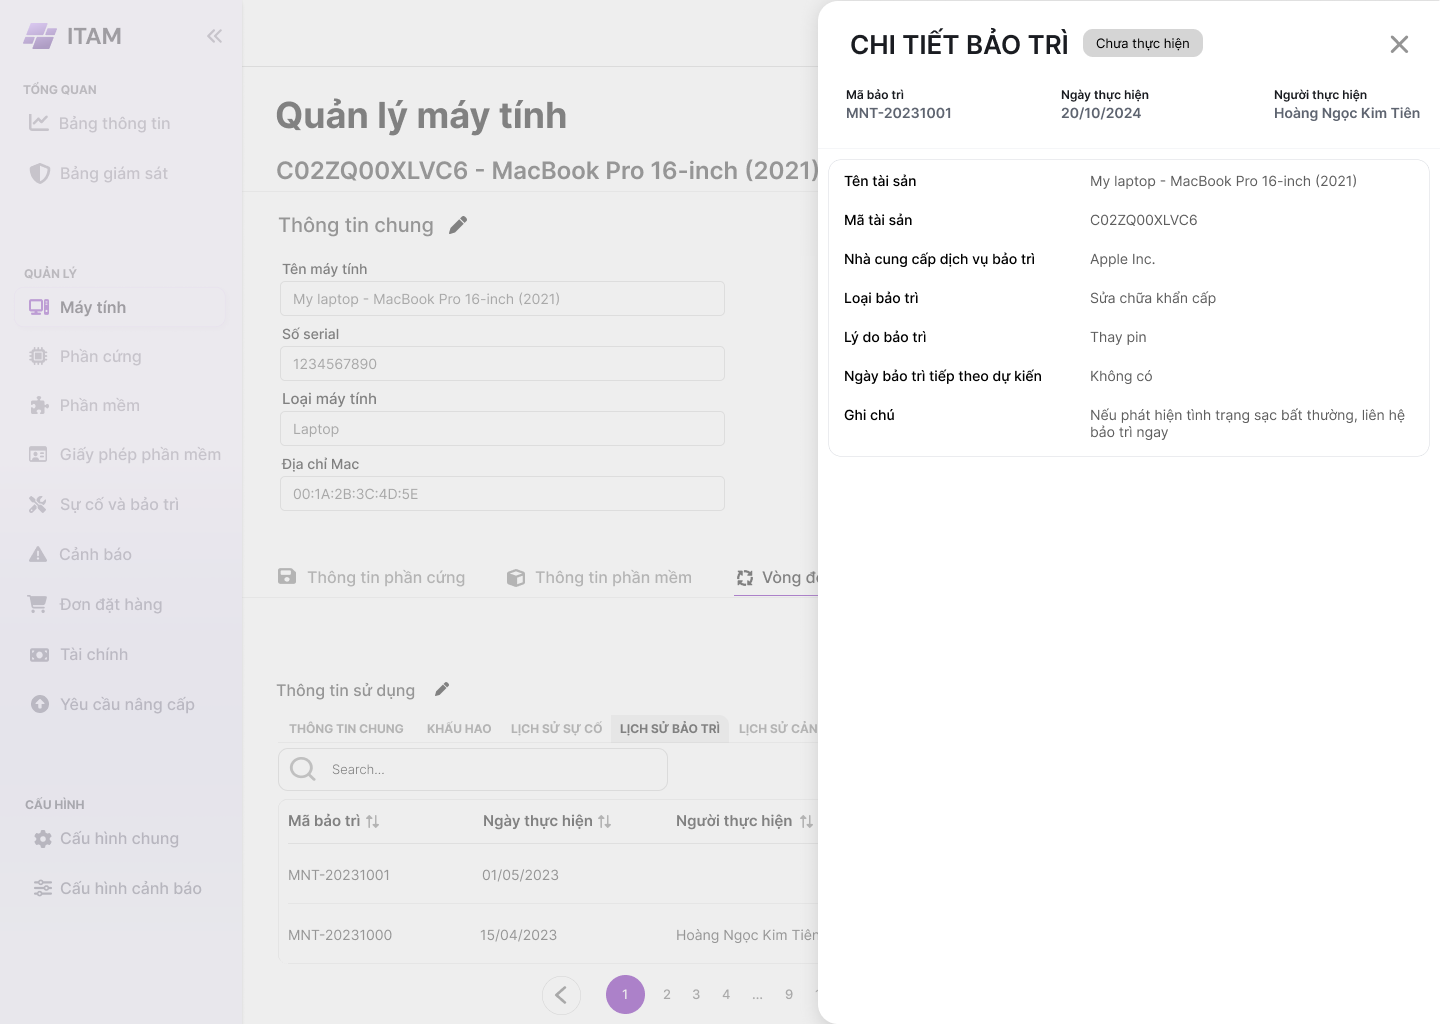
\includegraphics[width=14cm]{Images/C5/UI/Feature-Giám sát tài sản-Máy tính 6.10.png}
%     \vspace{15pt}
%     \caption{Giao diện Quản lý máy tính 18}
% \end{figure}
% \begin{figure}[H]
%     \centering
%     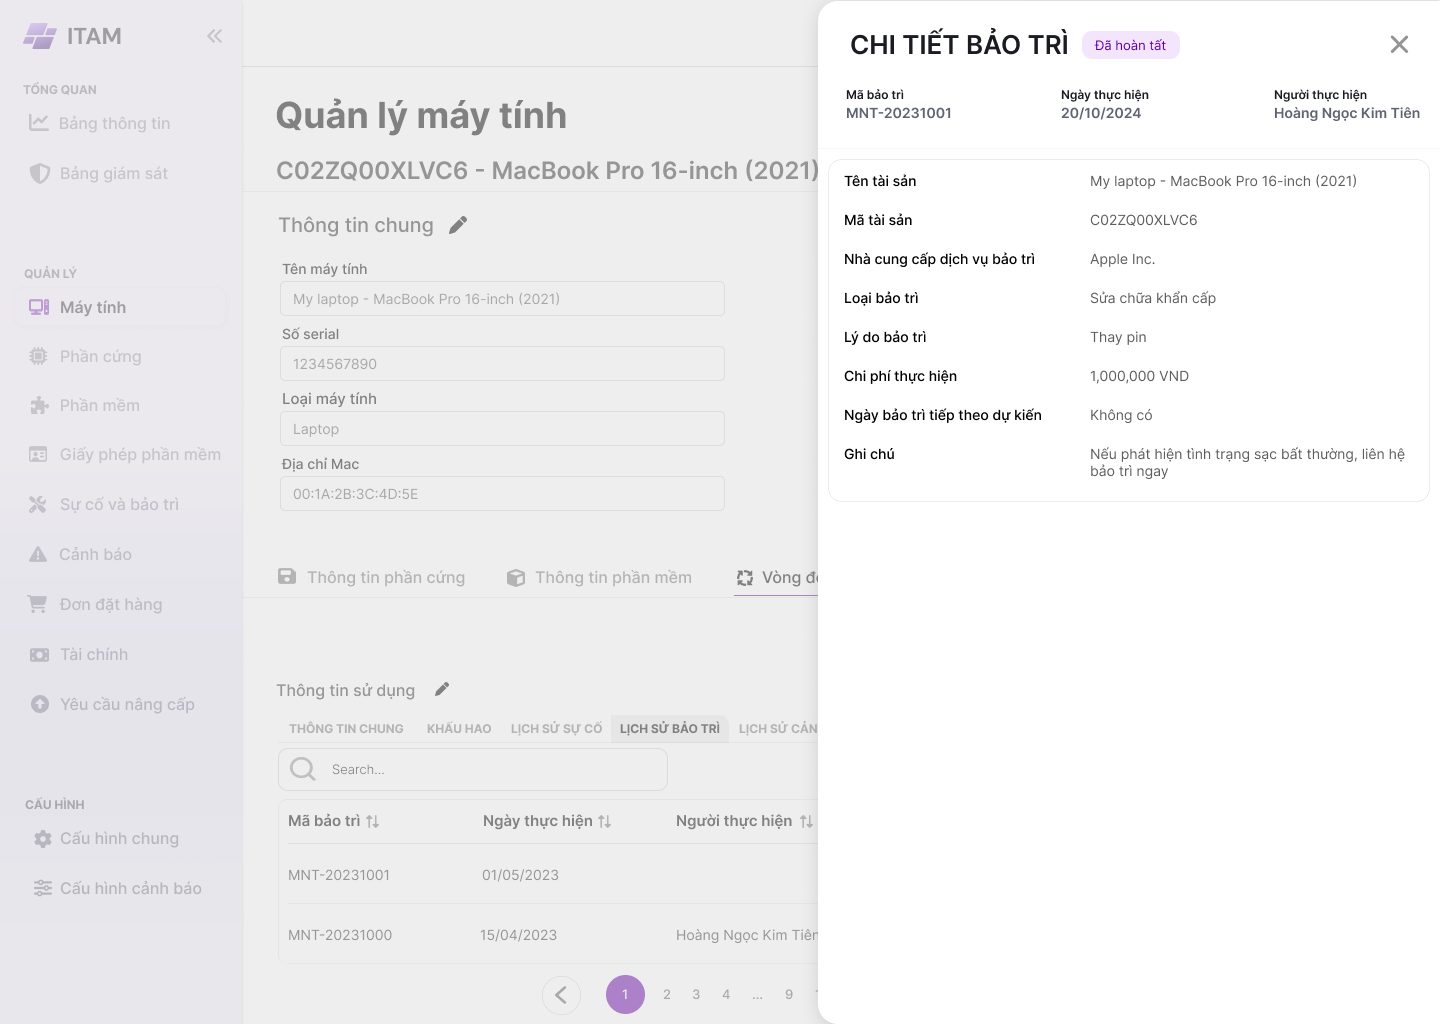
\includegraphics[width=14cm]{Images/C5/UI/Feature-Giám sát tài sản-Máy tính 6.11.png}
%     \vspace{15pt}
%     \caption{Giao diện Quản lý máy tính 19} 
% \end{figure}
% \begin{figure}[H]
%     \centering
%     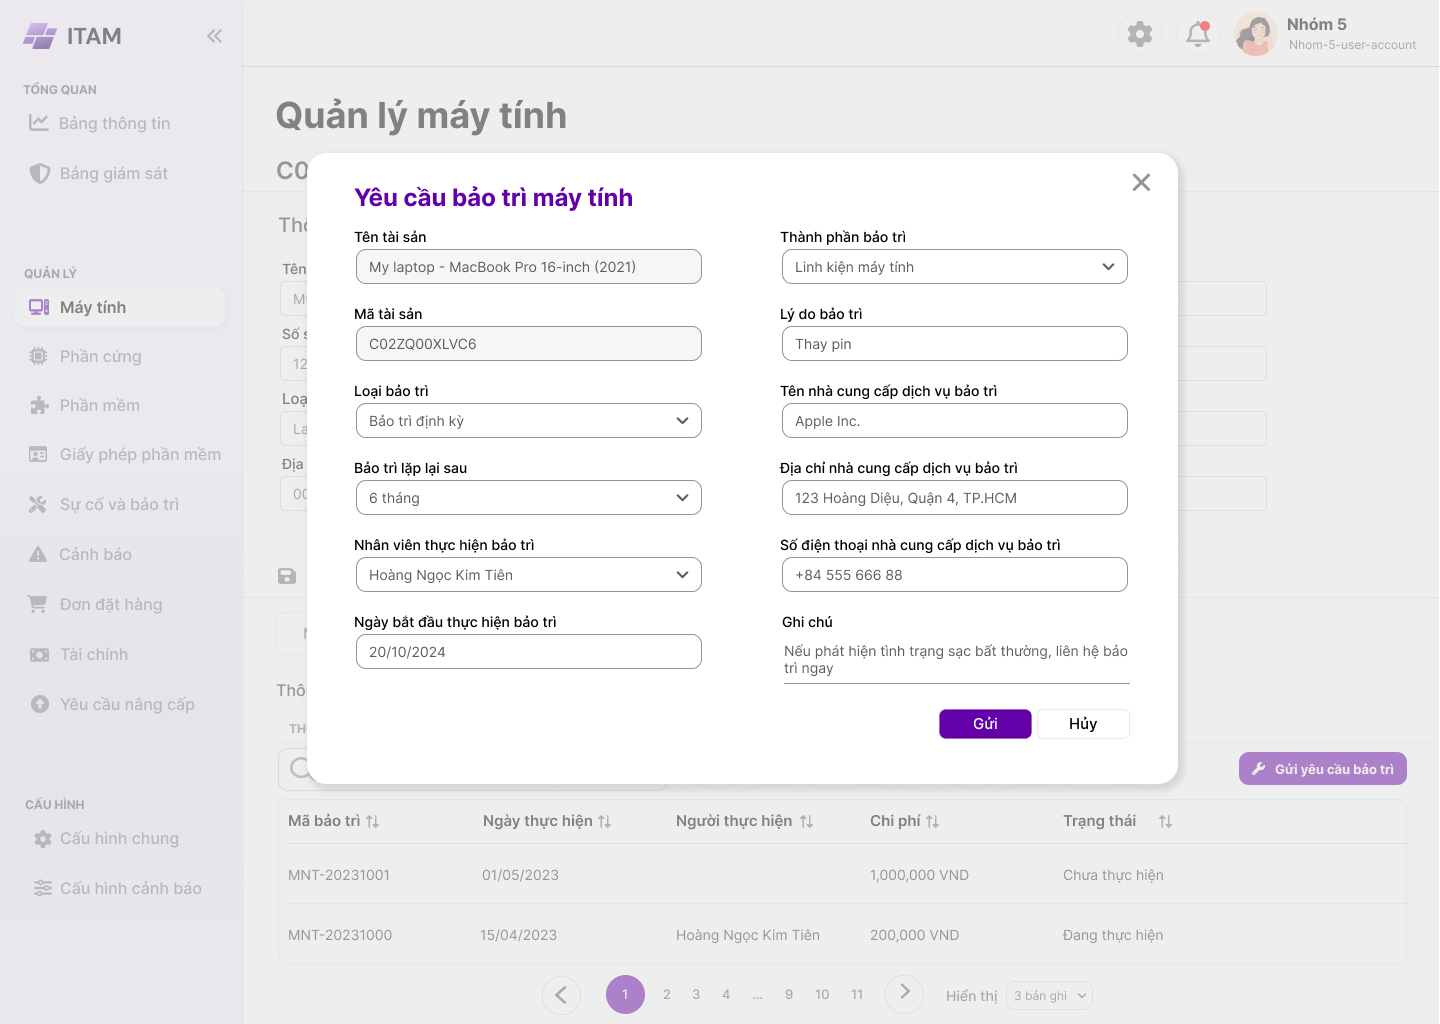
\includegraphics[width=14cm]{Images/C5/UI/Feature-Giám sát tài sản-Máy tính 6.12.png}
%     \vspace{15pt}
%     \caption{Giao diện Quản lý máy tính 11}
% \end{figure}
% \begin{figure}[H]
%     \centering
%     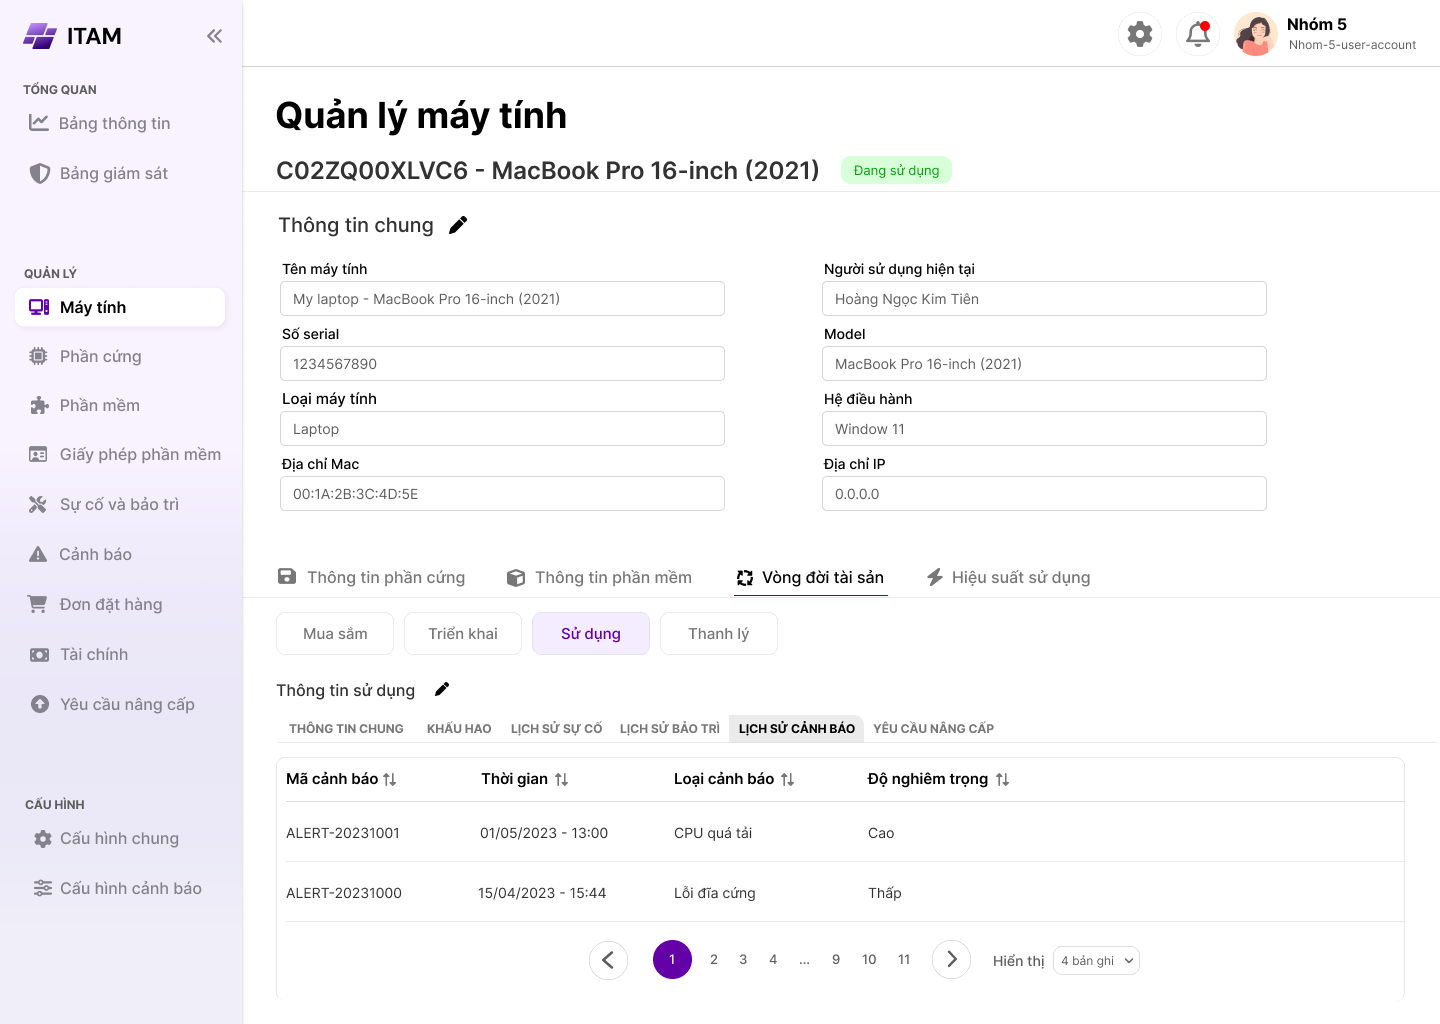
\includegraphics[width=14cm]{Images/C5/UI/Feature-Giám sát tài sản-Máy tính 6.13.png}
%     \vspace{15pt}
%     \caption{Giao diện Quản lý máy tính 15}
% \end{figure}
% \begin{figure}[H]
%     \centering
%     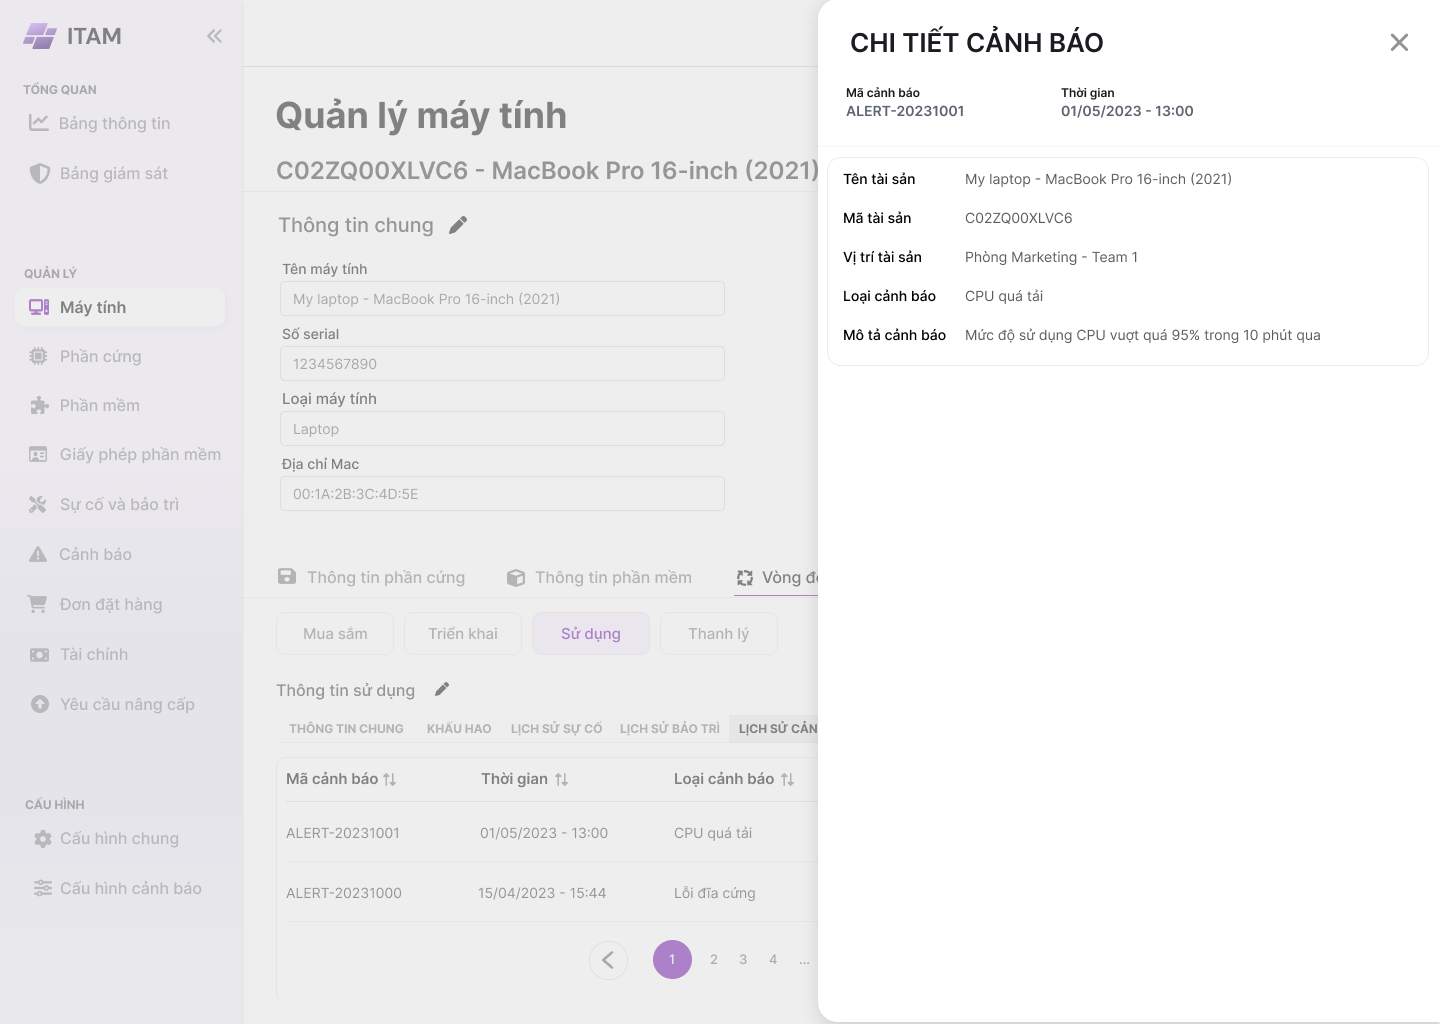
\includegraphics[width=14cm]{Images/C5/UI/Feature-Giám sát tài sản-Máy tính 6.14.png}
%     \vspace{15pt}
%     \caption{Giao diện Quản lý máy tính 22}
% \end{figure}
% \begin{figure}[H]
%     \centering
%     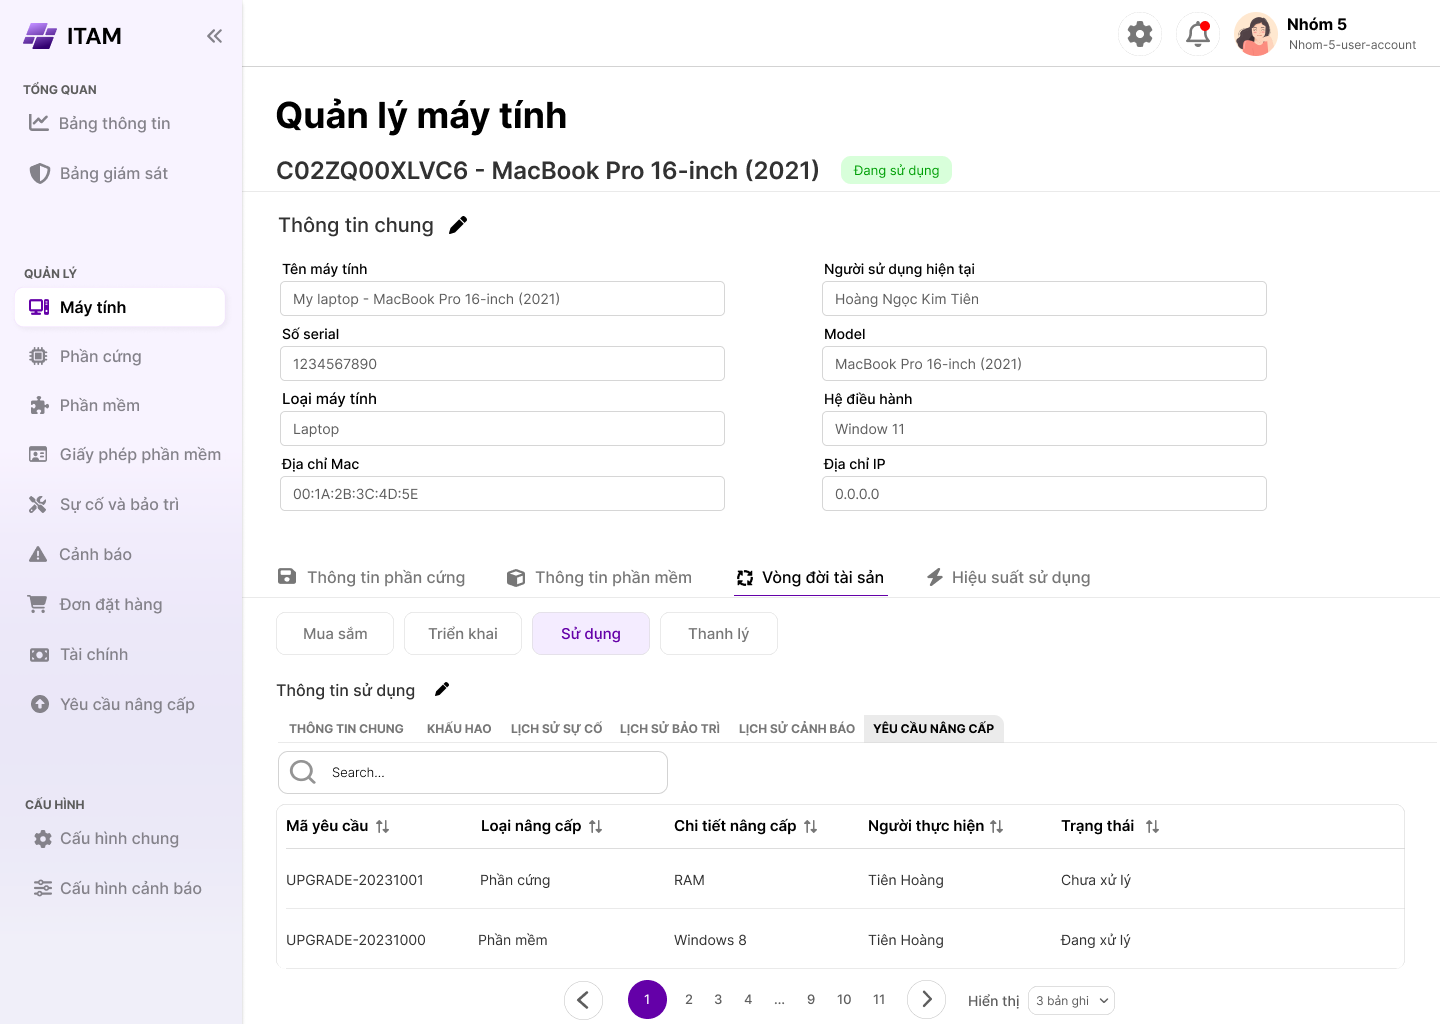
\includegraphics[width=14cm]{Images/C5/UI/Feature-Giám sát tài sản-Máy tính 6.15.png}
%     \vspace{15pt}
%     \caption{Giao diện Quản lý máy tính 16}
% \end{figure}
% \begin{figure}[H]
%     \centering
%     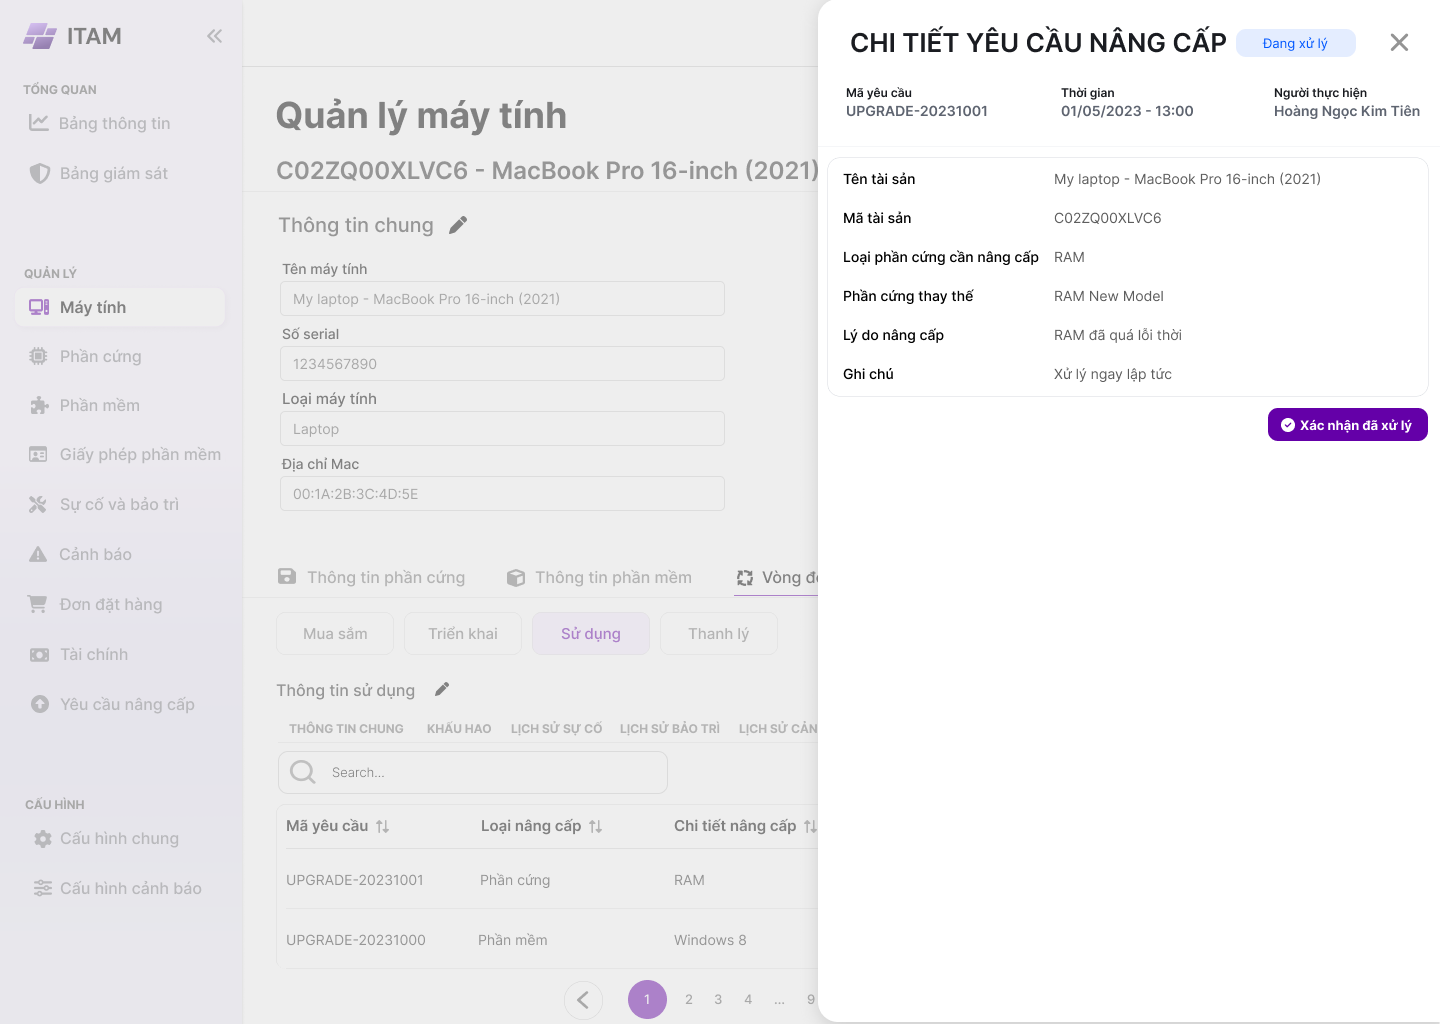
\includegraphics[width=14cm]{Images/C5/UI/Feature-Giám sát tài sản-Máy tính 6.16.png}
%     \vspace{15pt}
%     \caption{Giao diện Quản lý máy tính 24}
% \end{figure}
% \begin{figure}[H]
%     \centering
%     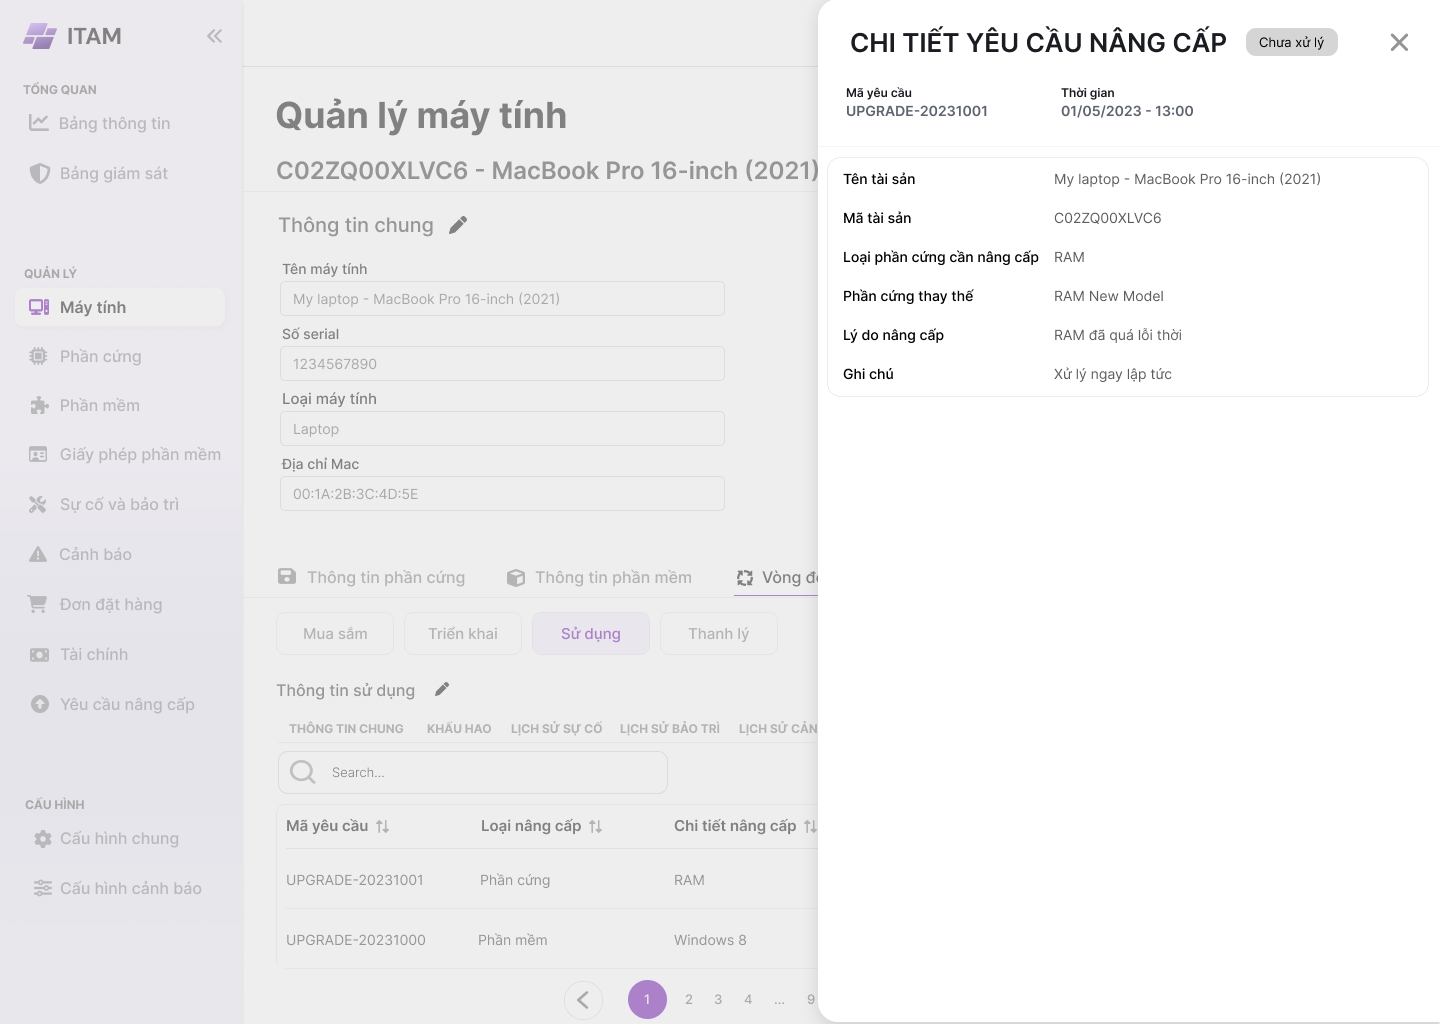
\includegraphics[width=14cm]{Images/C5/UI/Feature-Giám sát tài sản-Máy tính 6.17.png}
%     \vspace{15pt}
%     \caption{Giao diện Quản lý máy tính 25}
% \end{figure}
% \begin{figure}[H]
%     \centering
%     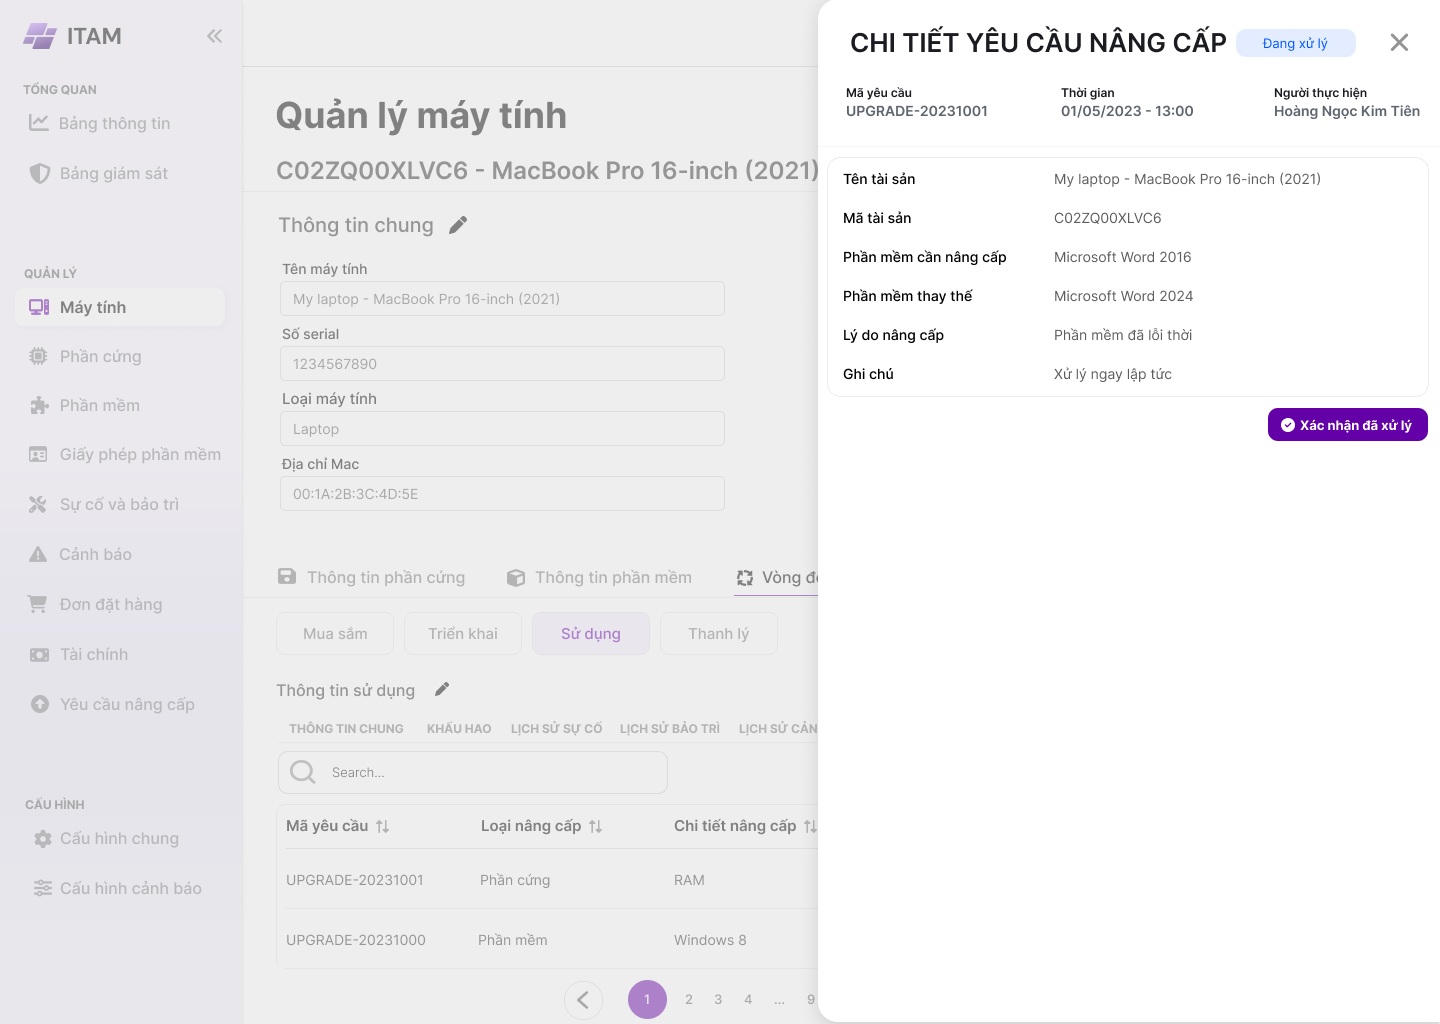
\includegraphics[width=14cm]{Images/C5/UI/Feature-Giám sát tài sản-Máy tính 6.18.png}
%     \vspace{15pt}
%     \caption{Giao diện Quản lý máy tính 26}
% \end{figure}
% \begin{figure}[H]
%     \centering
%     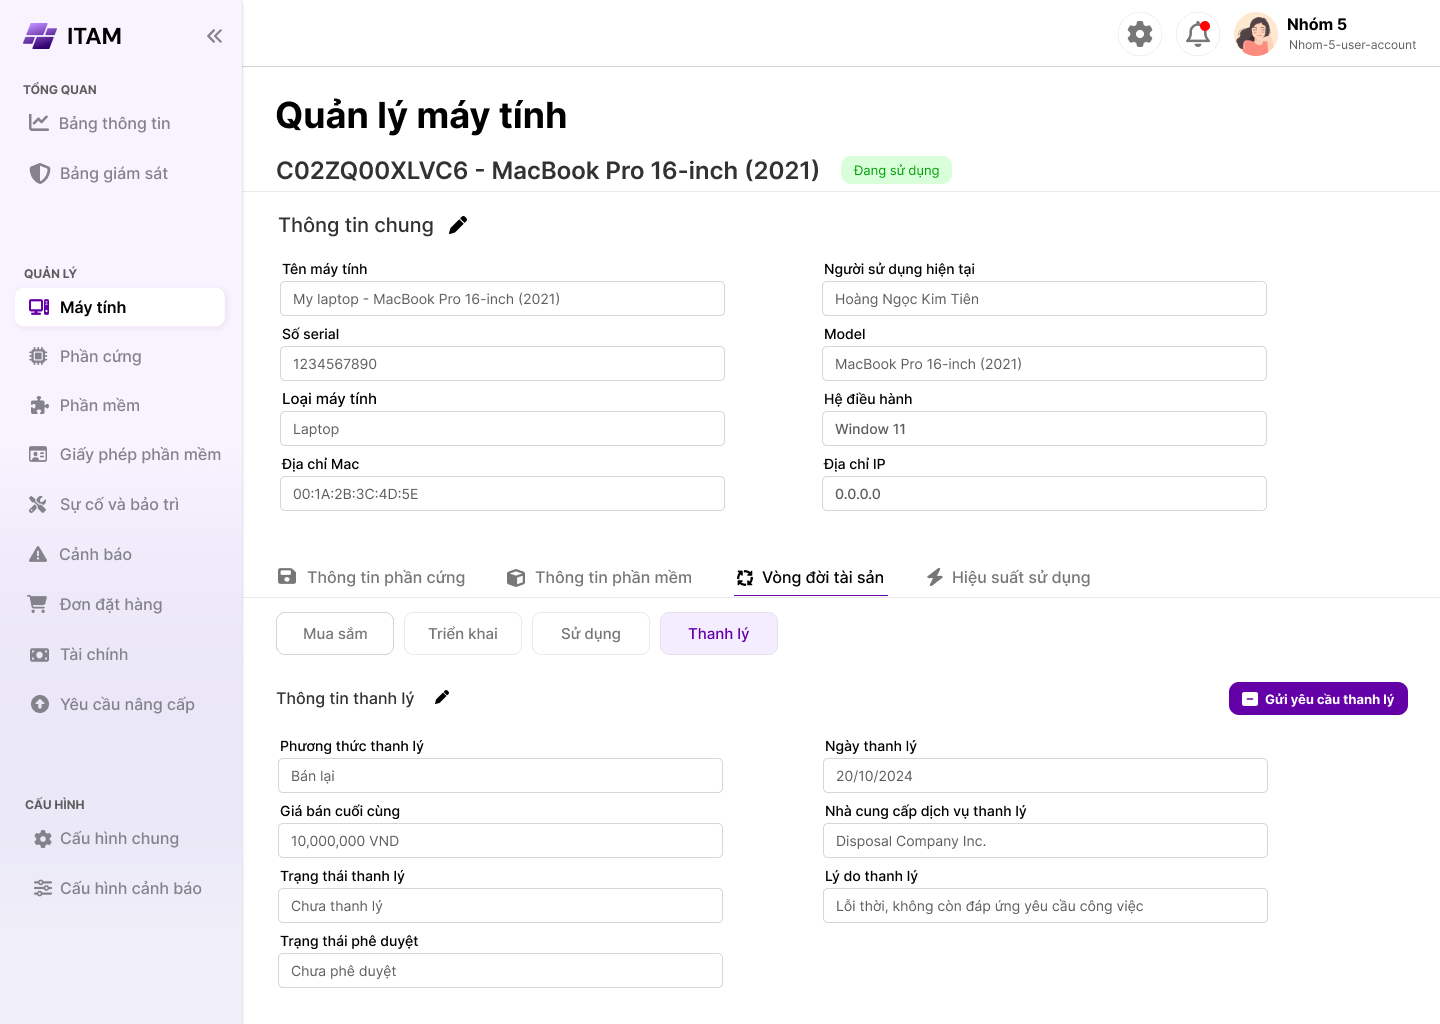
\includegraphics[width=14cm]{Images/C5/UI/Feature-Giám sát tài sản-Máy tính 7.1.png}
%     \vspace{15pt}
%     \caption{Giao diện Quản lý máy tính 12}
% \end{figure}
% \begin{figure}[H]
%     \centering
%     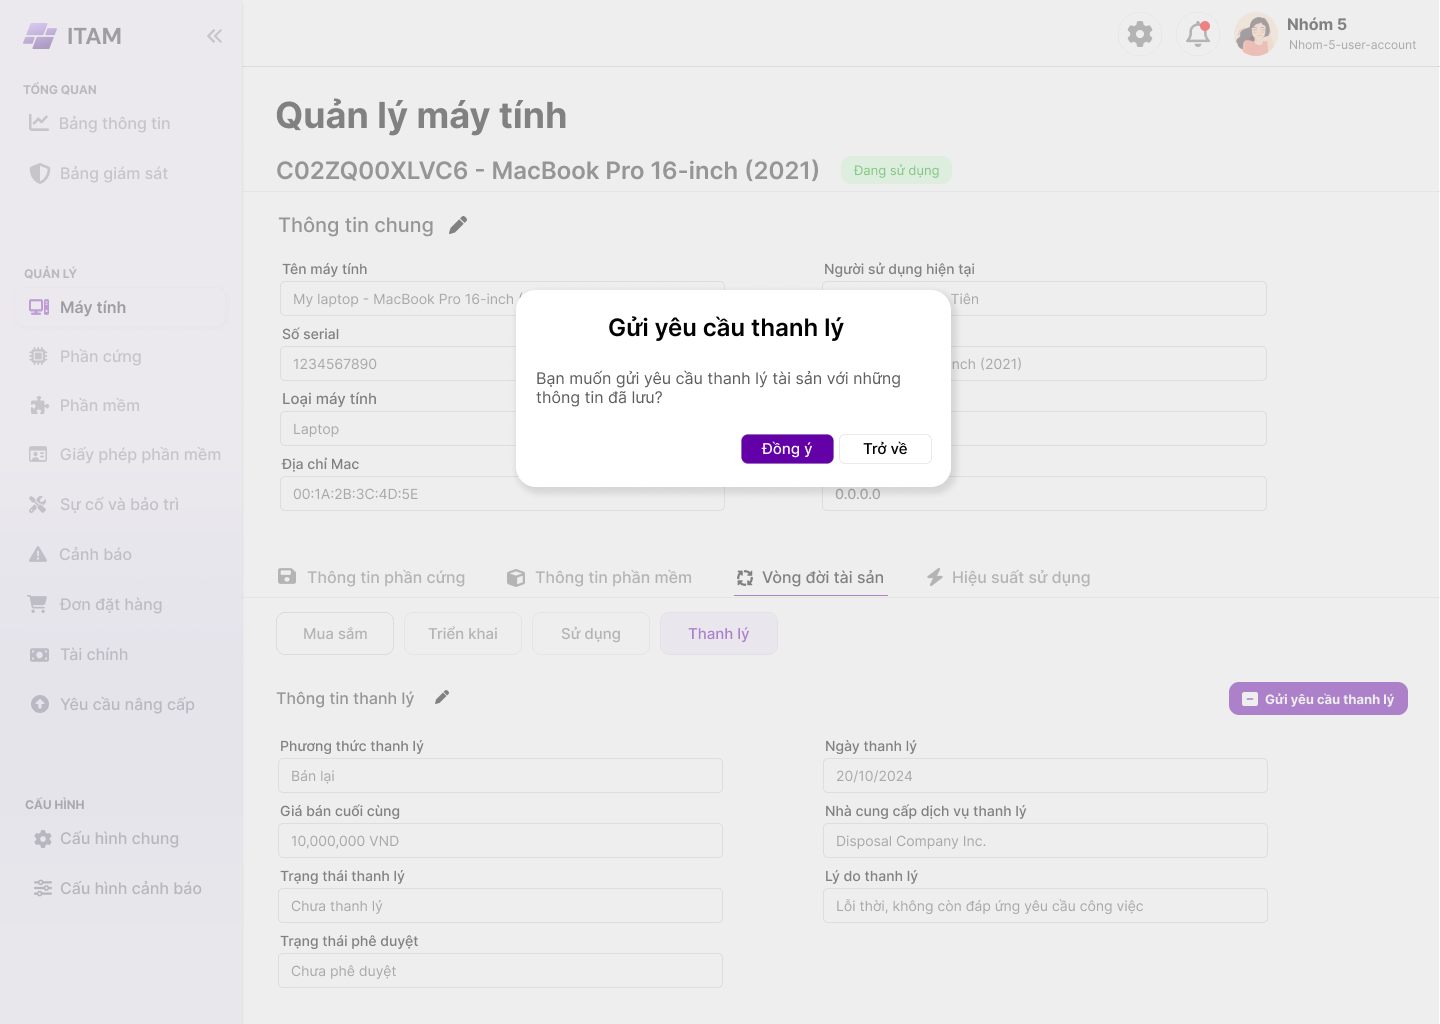
\includegraphics[width=14cm]{Images/C5/UI/Feature-Giám sát tài sản-Máy tính 7.2.png}
%     \vspace{15pt}
%     \caption{Giao diện Quản lý máy tính 28}
% \end{figure}
% \begin{figure}[H]
%     \centering
%     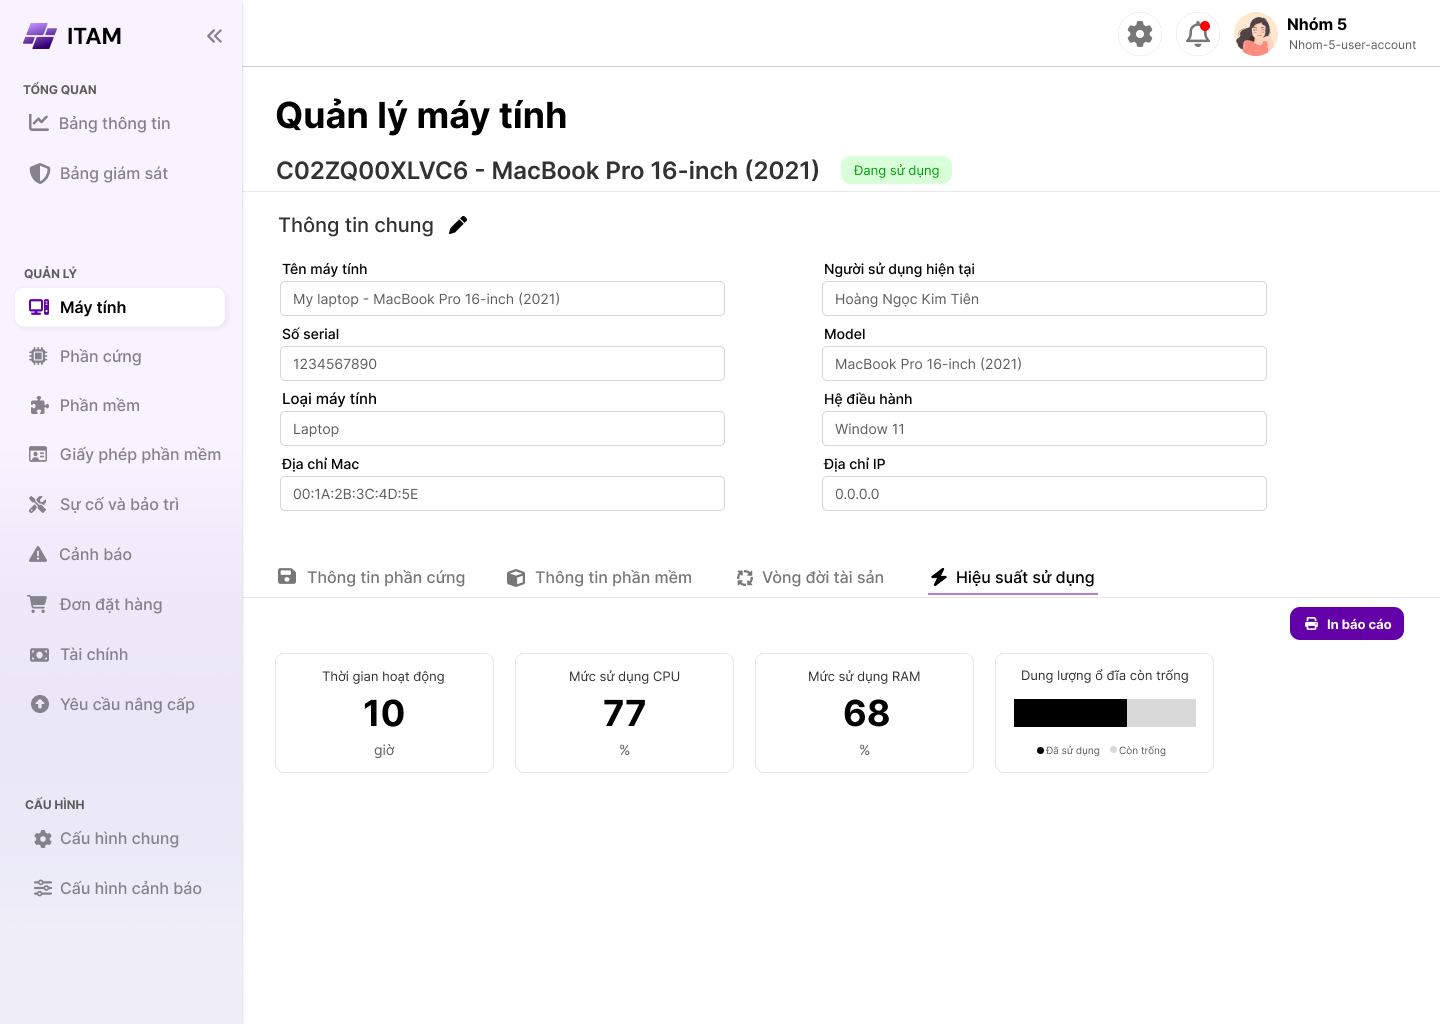
\includegraphics[width=14cm]{Images/C5/UI/Feature-Giám sát tài sản-Máy tính 9.1.png}
%     \vspace{15pt}
%     \caption{Giao diện Quản lý máy tính 2}
% \end{figure}
\begin{figure}[H]
    \centering
    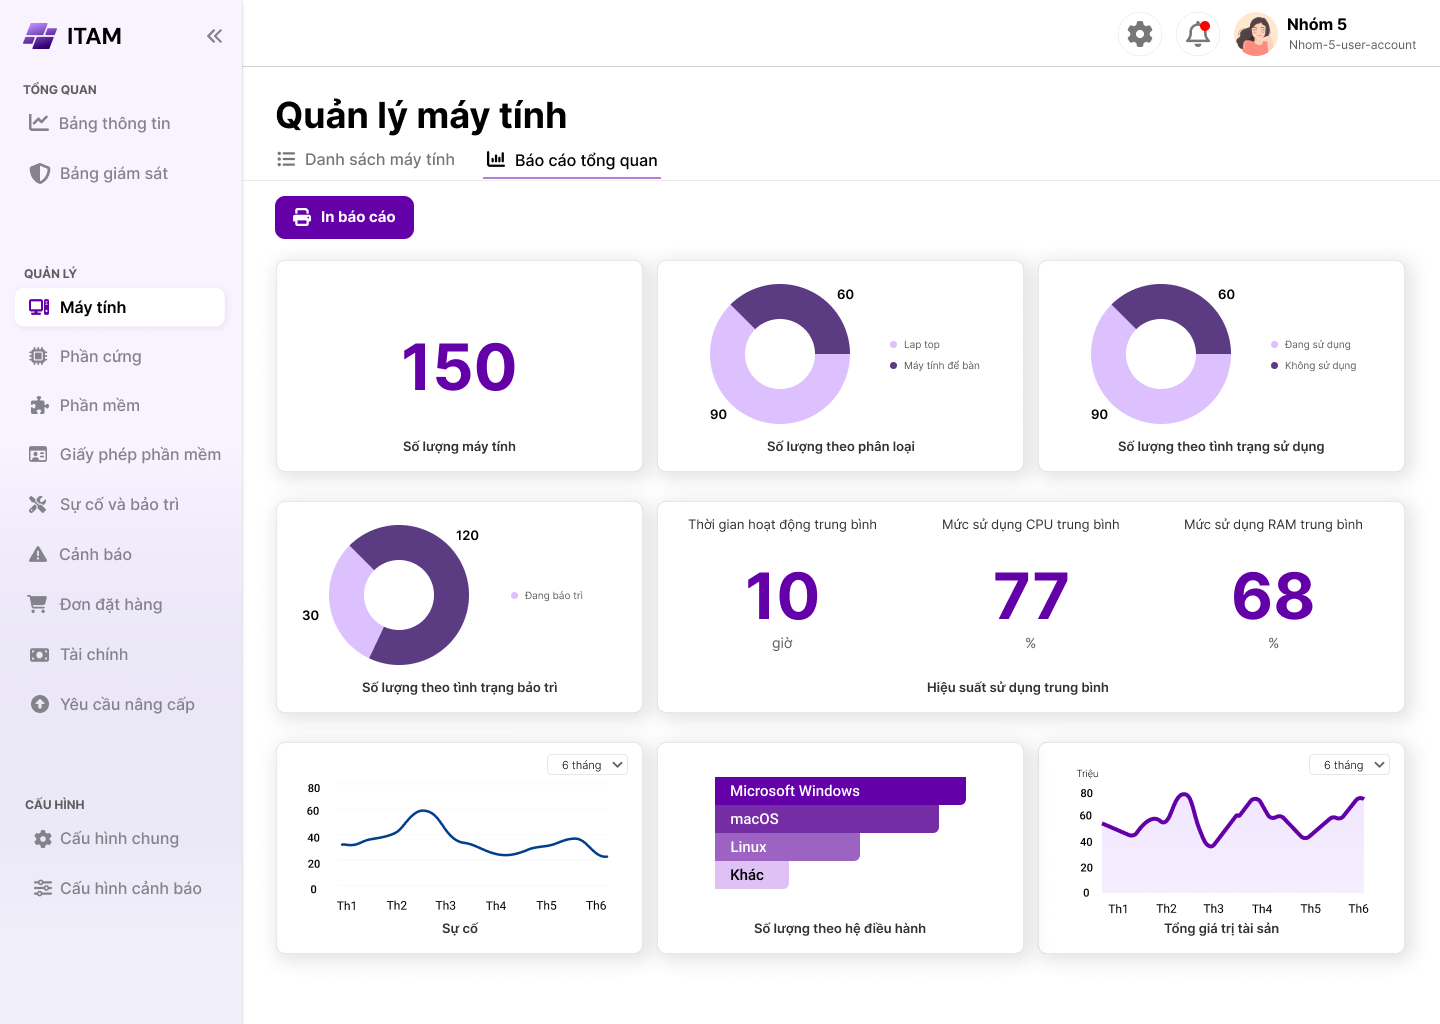
\includegraphics[width=14cm]{Images/C5/UI/Feature-Giám sát tài sản-Máy tính 10.png}
    \vspace{15pt}
    \caption{Giao diện Quản lý máy tính 2}
\end{figure}

\item{Quản lý phần cứng}\\
Ở chức năng Quản lý phần cứng, người dùng có thể dễ dàng xem danh sách tất cả các phần cứng trong hệ thống, thêm mới phần cứng, xem chi tiết phần cứng, gửi yêu cầu bảo trì cho phần cứng, và xem báo cáo tổng quan về phần cứng (xem thêm chi tiết ở phụ lục).
% \begin{figure}[H]
%     \centering
%     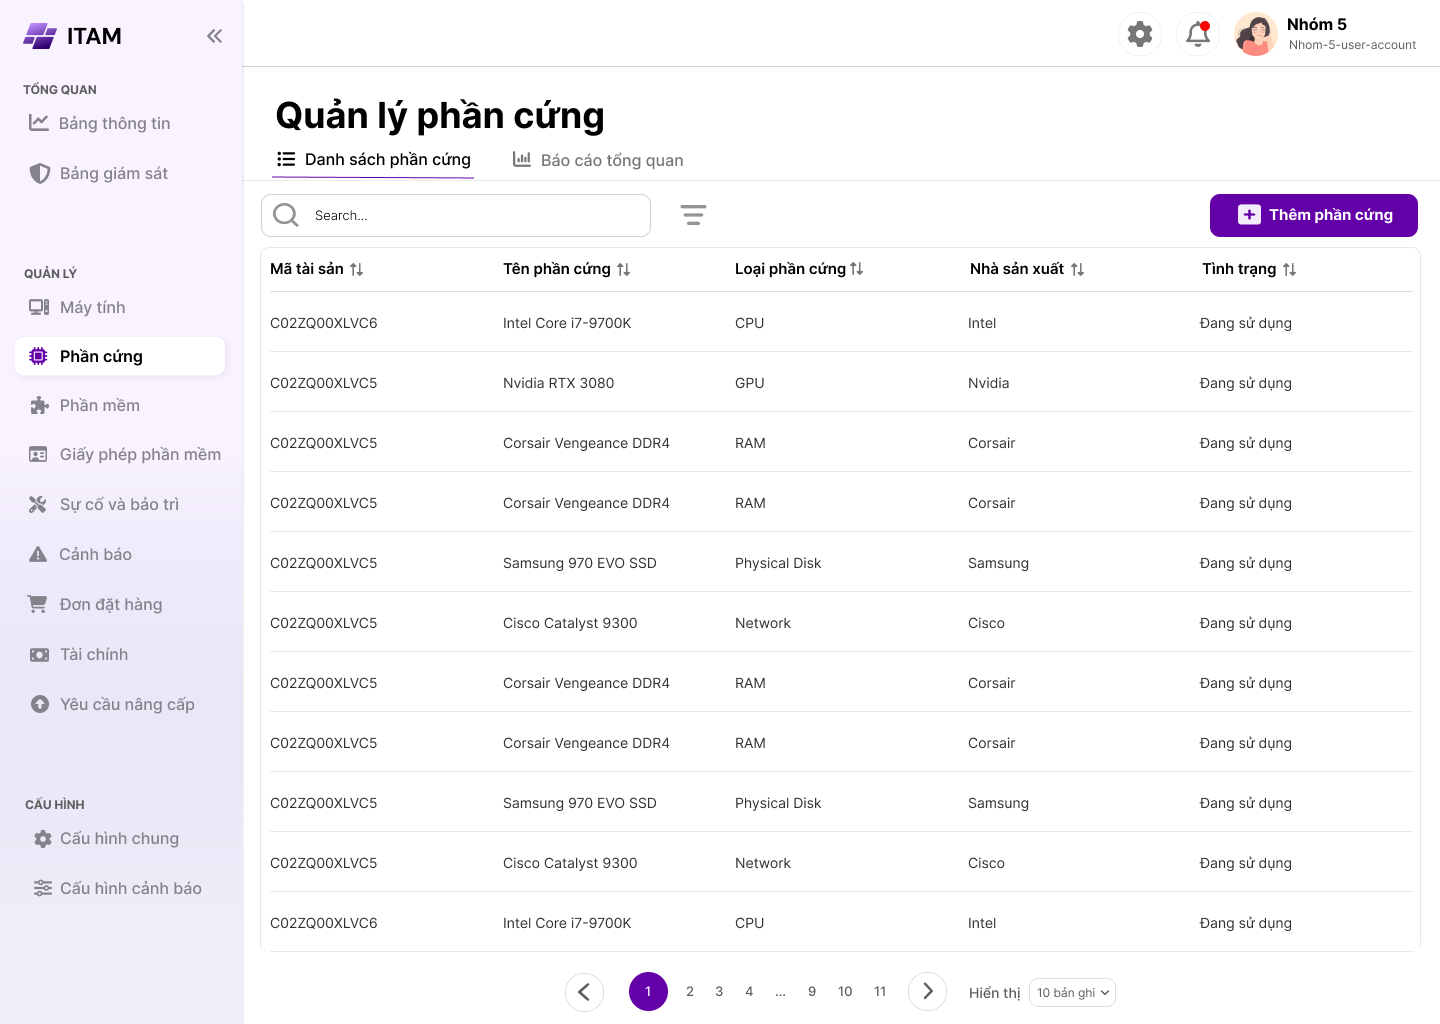
\includegraphics[width=14cm]{Images/C5/UI/Feature-Giám sát tài sản-Phần cứng 1.png}
%     \vspace{15pt}
%     \caption{Giao diện Quản lý phần cứng 1}
% \end{figure}
% \begin{figure}[H]
%     \centering
%     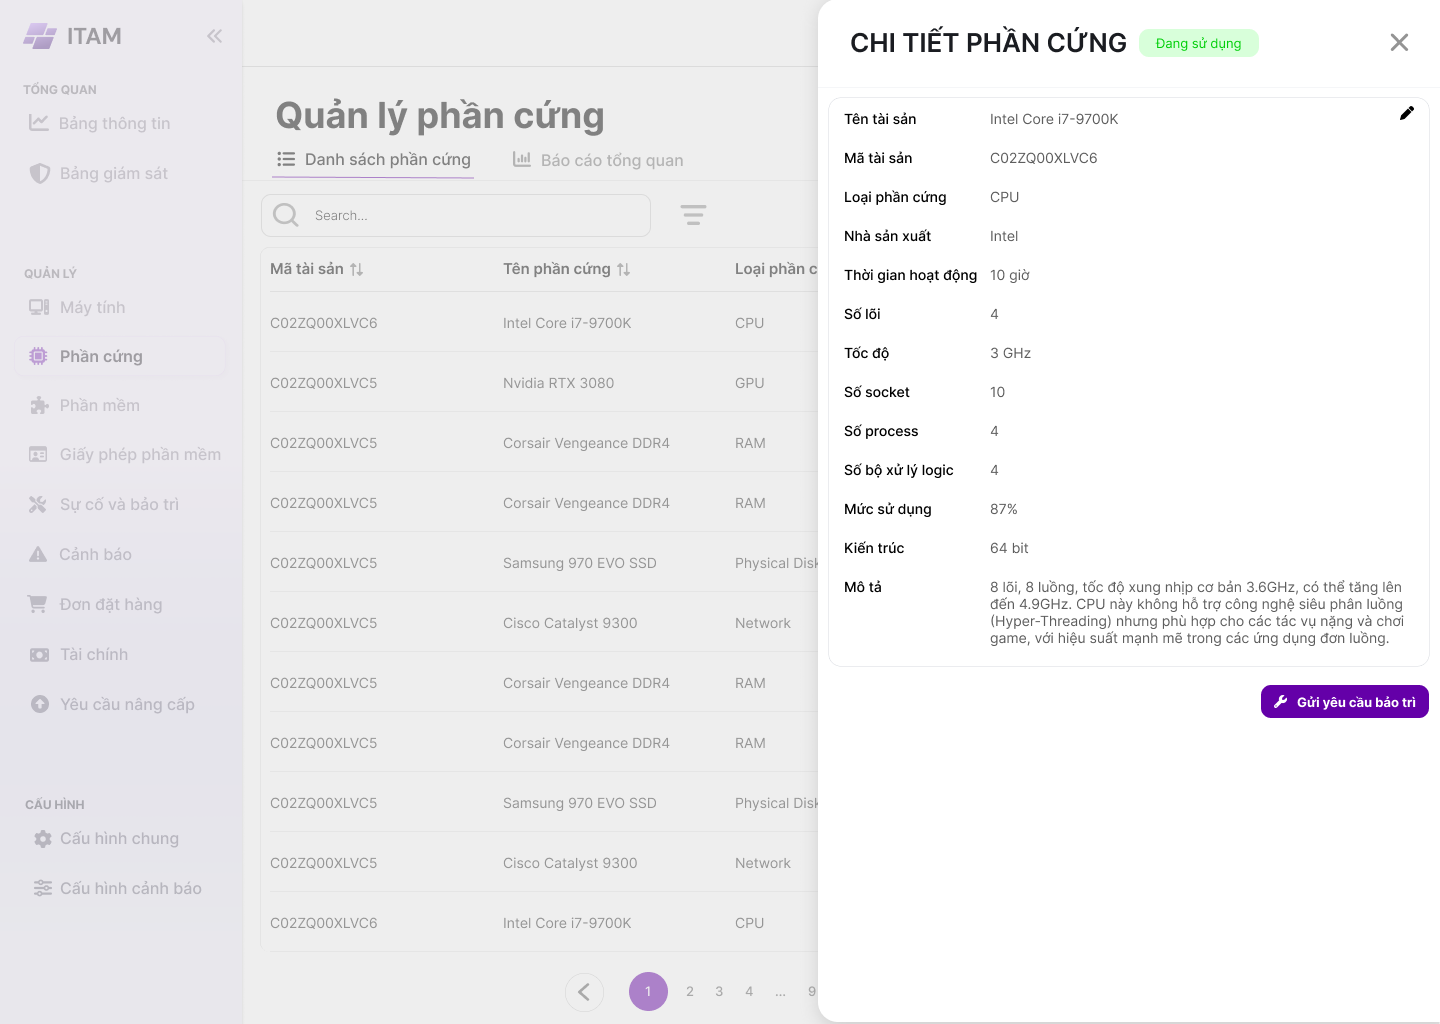
\includegraphics[width=14cm]{Images/C5/UI/Feature-Giám sát tài sản-Phần cứng 2.1-CPU.png}
%     \vspace{15pt}
%     \caption{Giao diện Quản lý phần cứng 2}
% \end{figure}
% \begin{figure}[H]
%     \centering
%     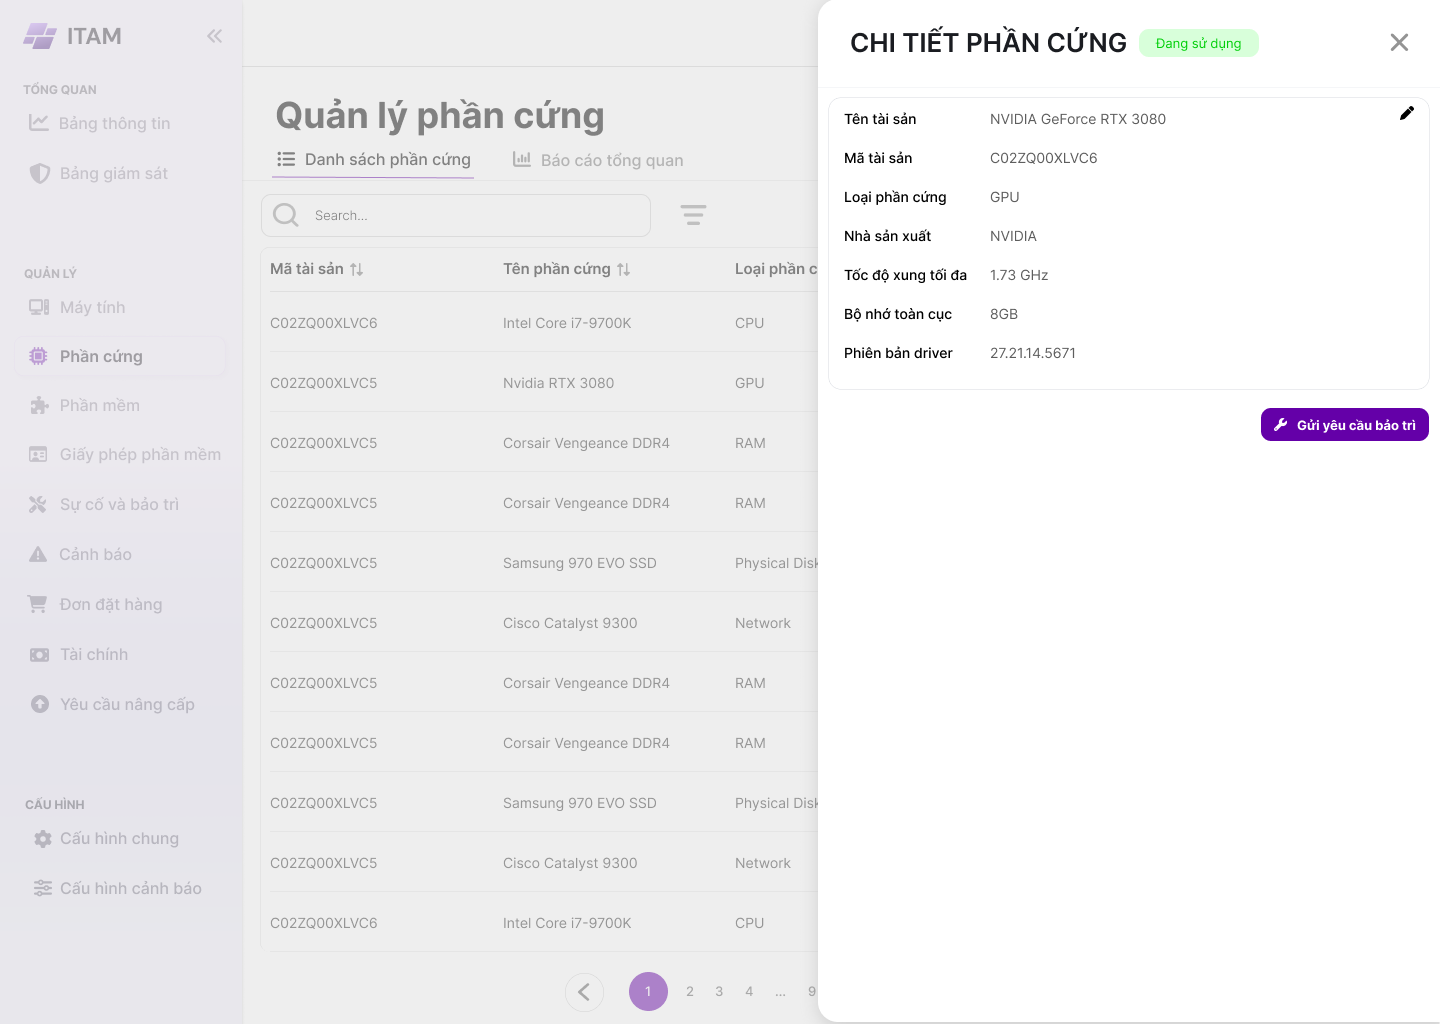
\includegraphics[width=14cm]{Images/C5/UI/Feature-Giám sát tài sản-Phần cứng 2.2-GPU.png}
%     \vspace{15pt}
%     \caption{Giao diện Quản lý phần cứng 3}
% \end{figure}
% \begin{figure}[H]
%     \centering
%     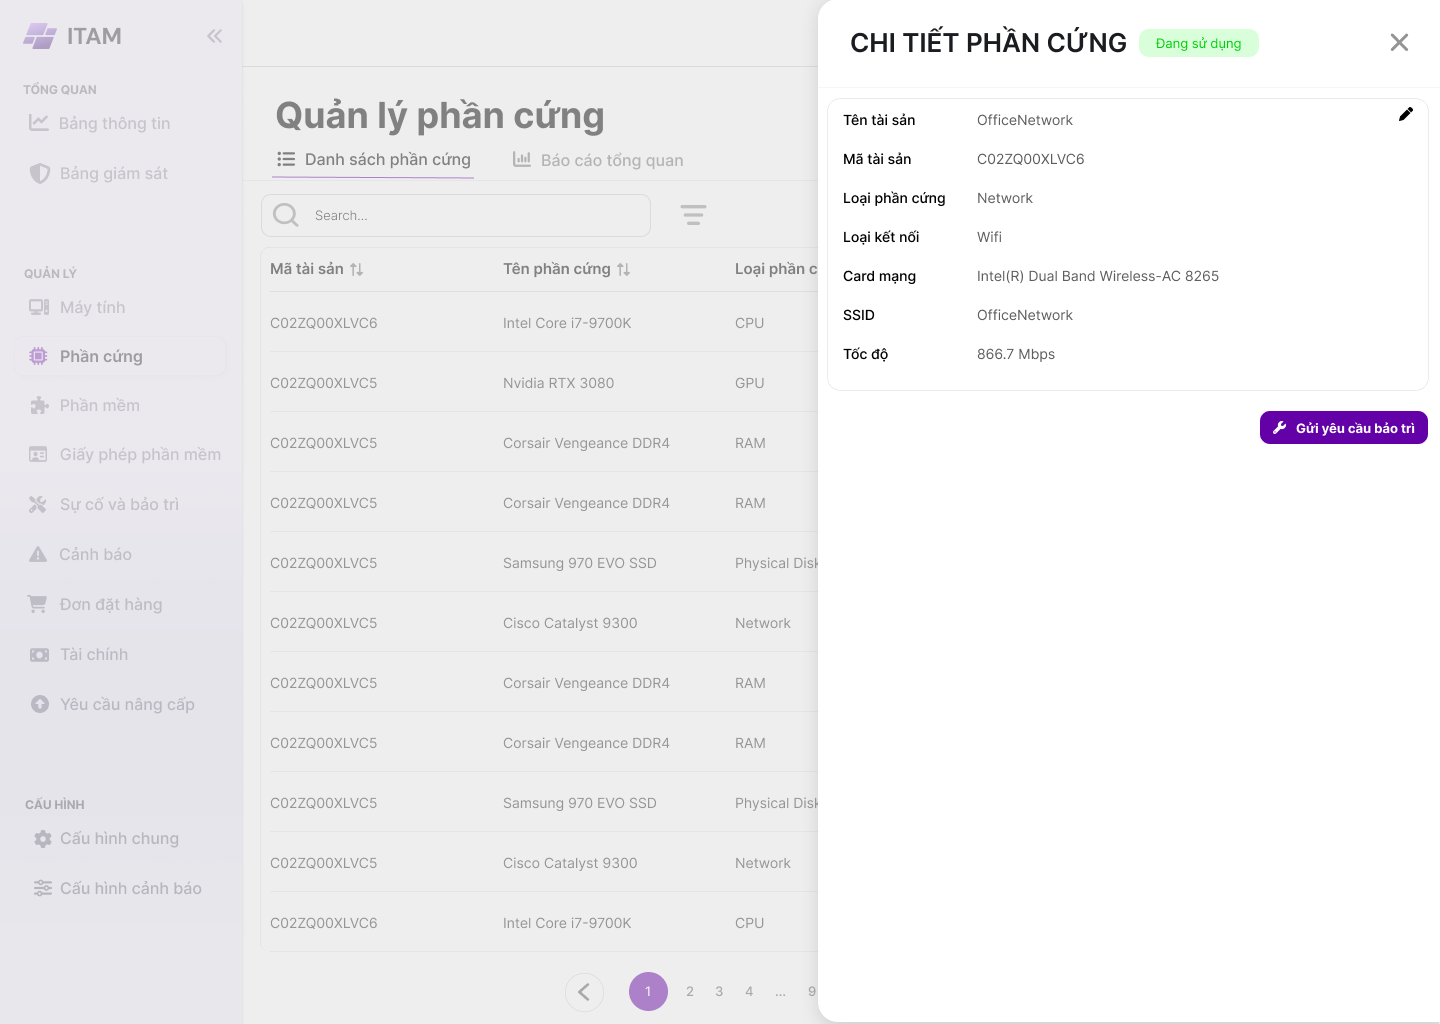
\includegraphics[width=14cm]{Images/C5/UI/Feature-Giám sát tài sản-Phần cứng 2.3-Network.png}
%     \vspace{15pt}
%     \caption{Giao diện Quản lý phần cứng 4}
% \end{figure}
% \begin{figure}[H]
%     \centering
%     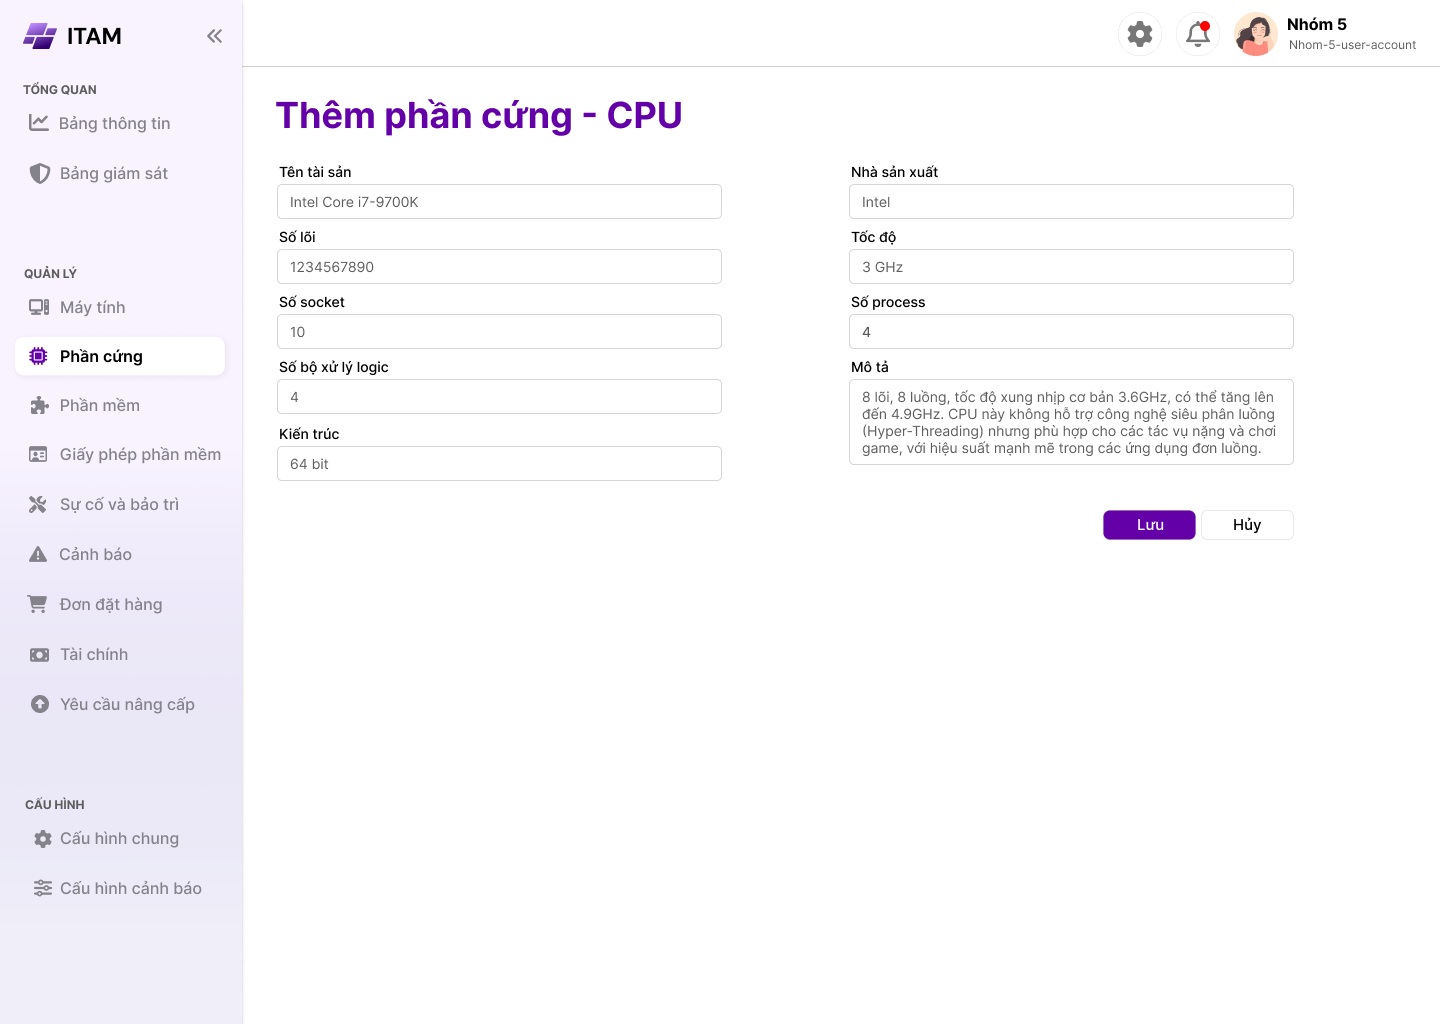
\includegraphics[width=14cm]{Images/C5/UI/Feature-Giám sát tài sản-Phần cứng 4.2.png}
%     \vspace{15pt}
%     \caption{Giao diện Quản lý phần cứng 3}
% \end{figure}
% \begin{figure}[H]
%     \centering
%     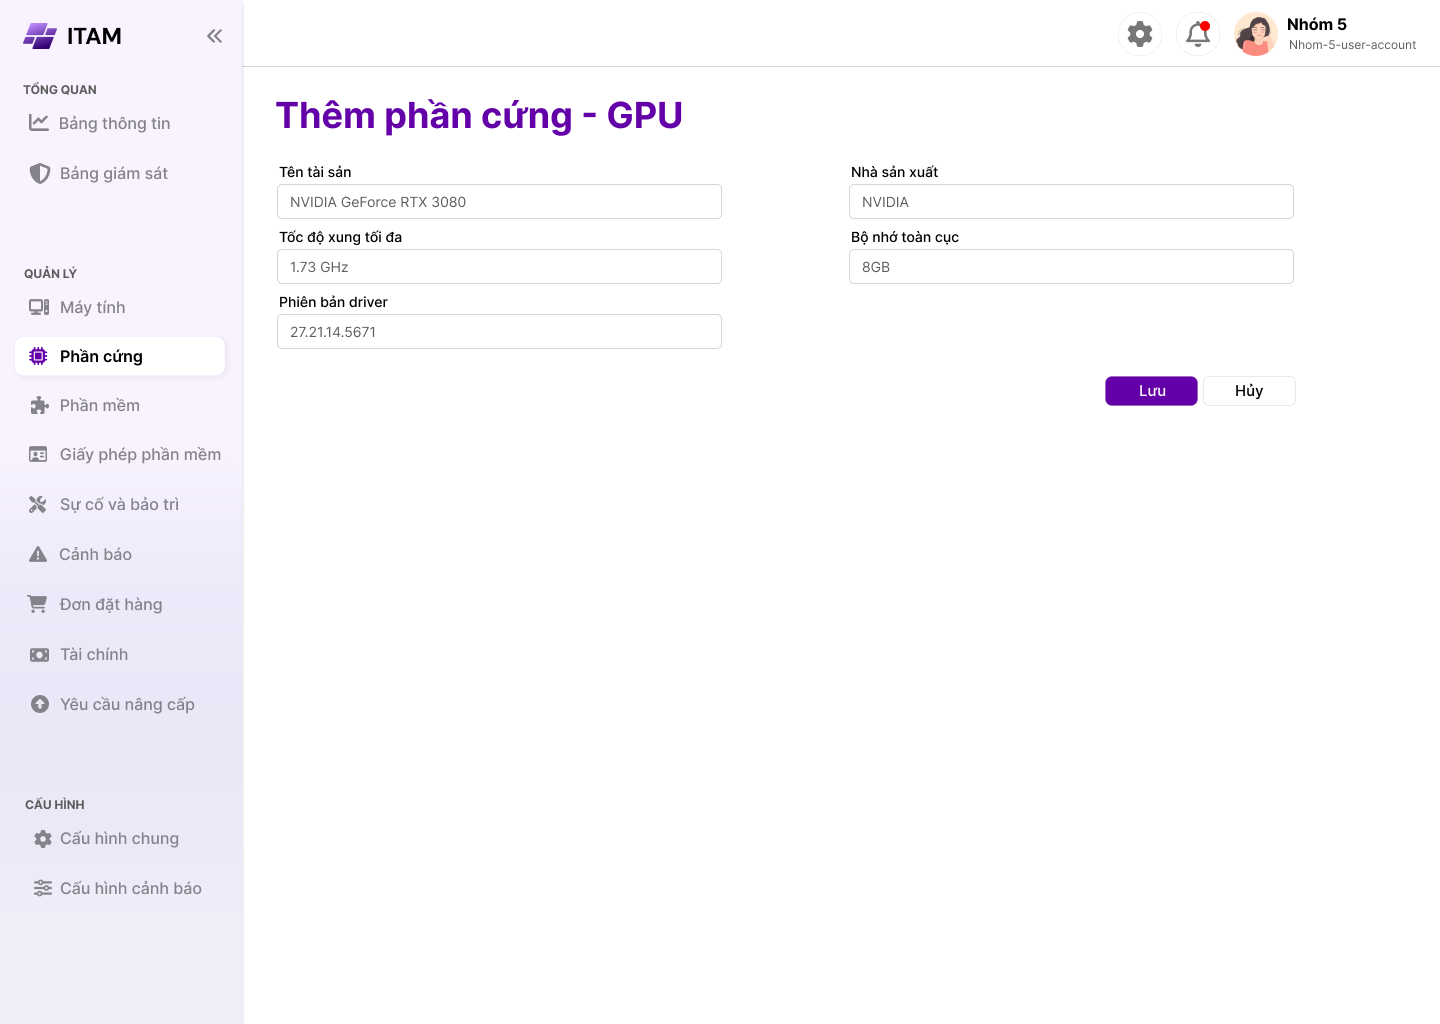
\includegraphics[width=14cm]{Images/C5/UI/Feature-Giám sát tài sản-Phần cứng 4.3.png}
%     \vspace{15pt}
%     \caption{Giao diện Quản lý phần cứng 6}
% \end{figure}
% \begin{figure}[H]
%     \centering
%     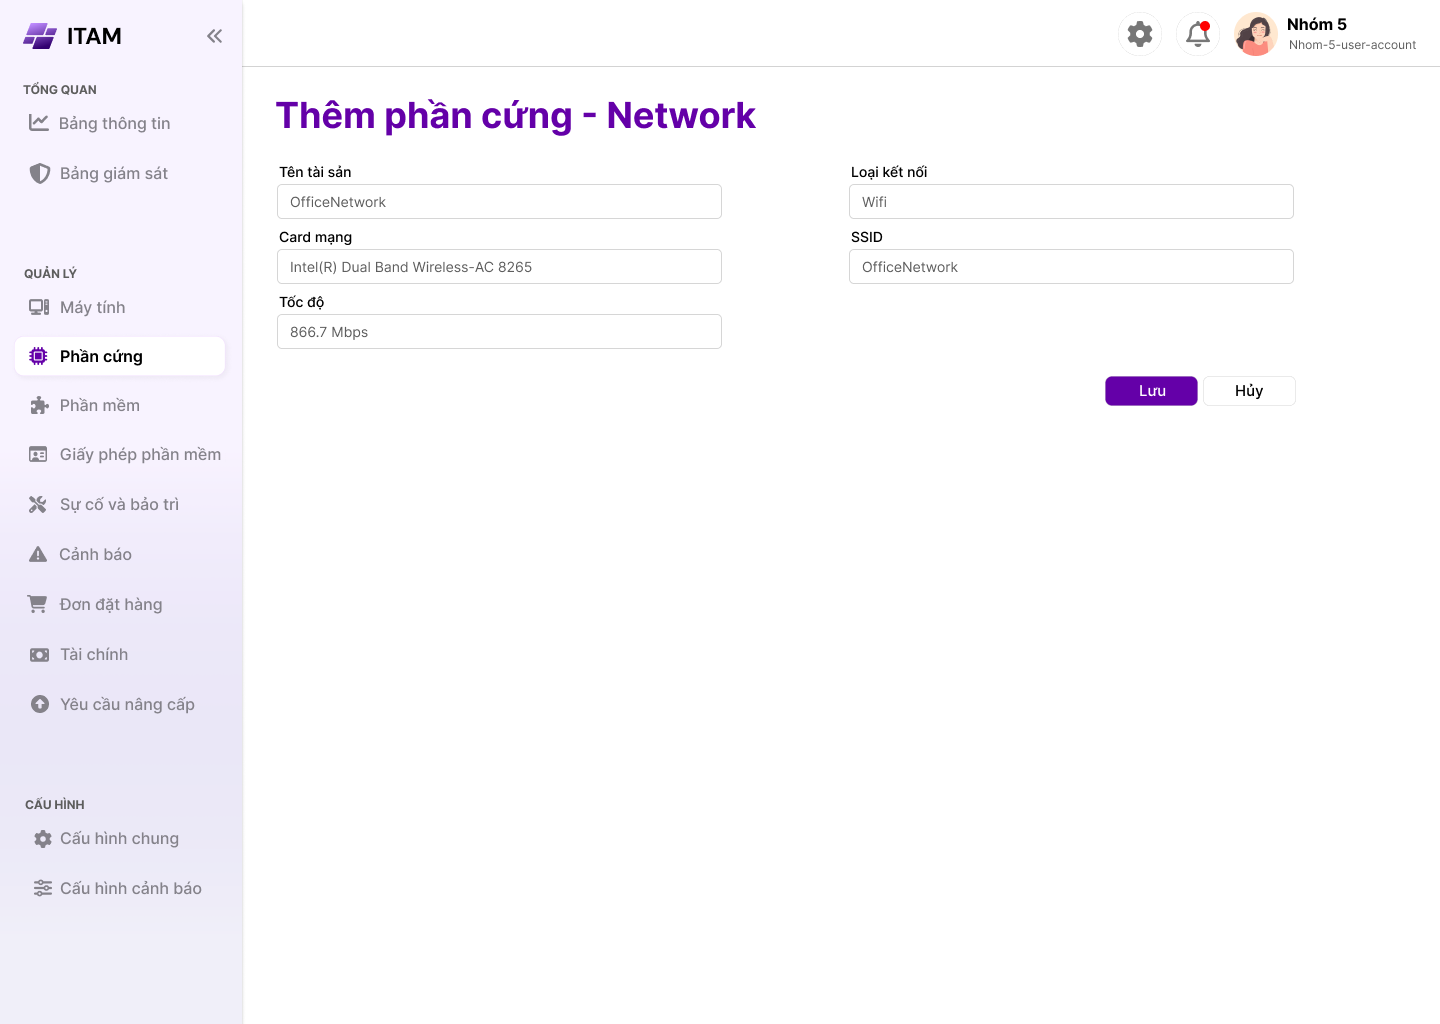
\includegraphics[width=14cm]{Images/C5/UI/Feature-Giám sát tài sản-Phần cứng 4.4.png}
%     \vspace{15pt}
%     \caption{Giao diện Quản lý phần cứng 7}
% \end{figure}
% \begin{figure}[H]
%     \centering
%     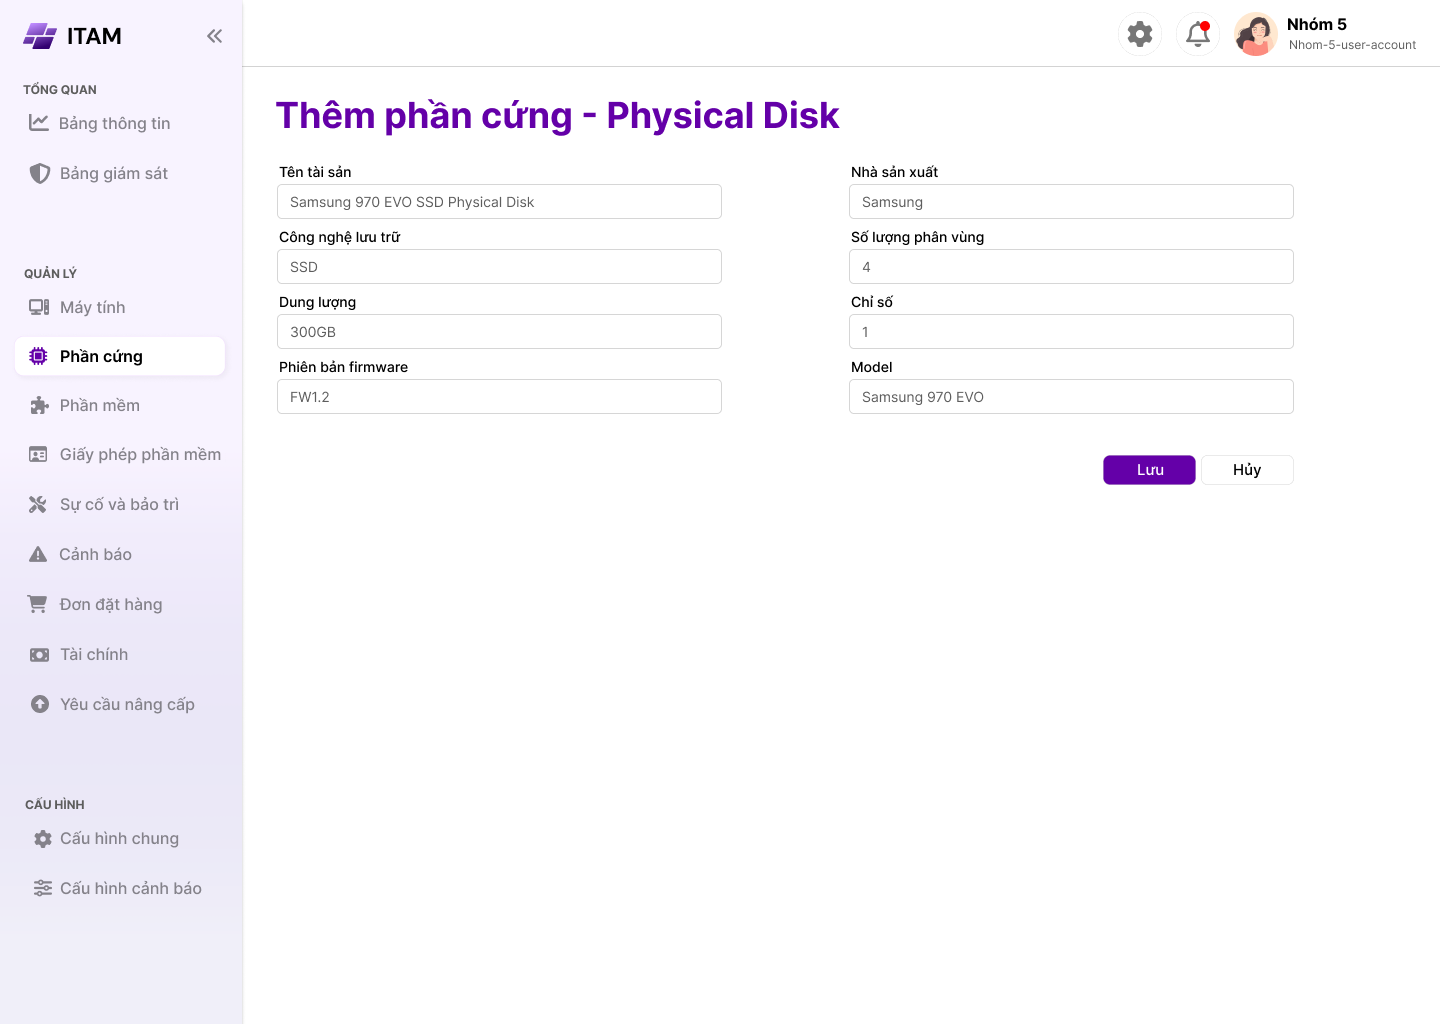
\includegraphics[width=14cm]{Images/C5/UI/Feature-Giám sát tài sản-Phần cứng 4.5.png}
%     \vspace{15pt}
%     \caption{Giao diện Quản lý phần cứng 8}
% \end{figure}
% \begin{figure}[H]
%     \centering
%     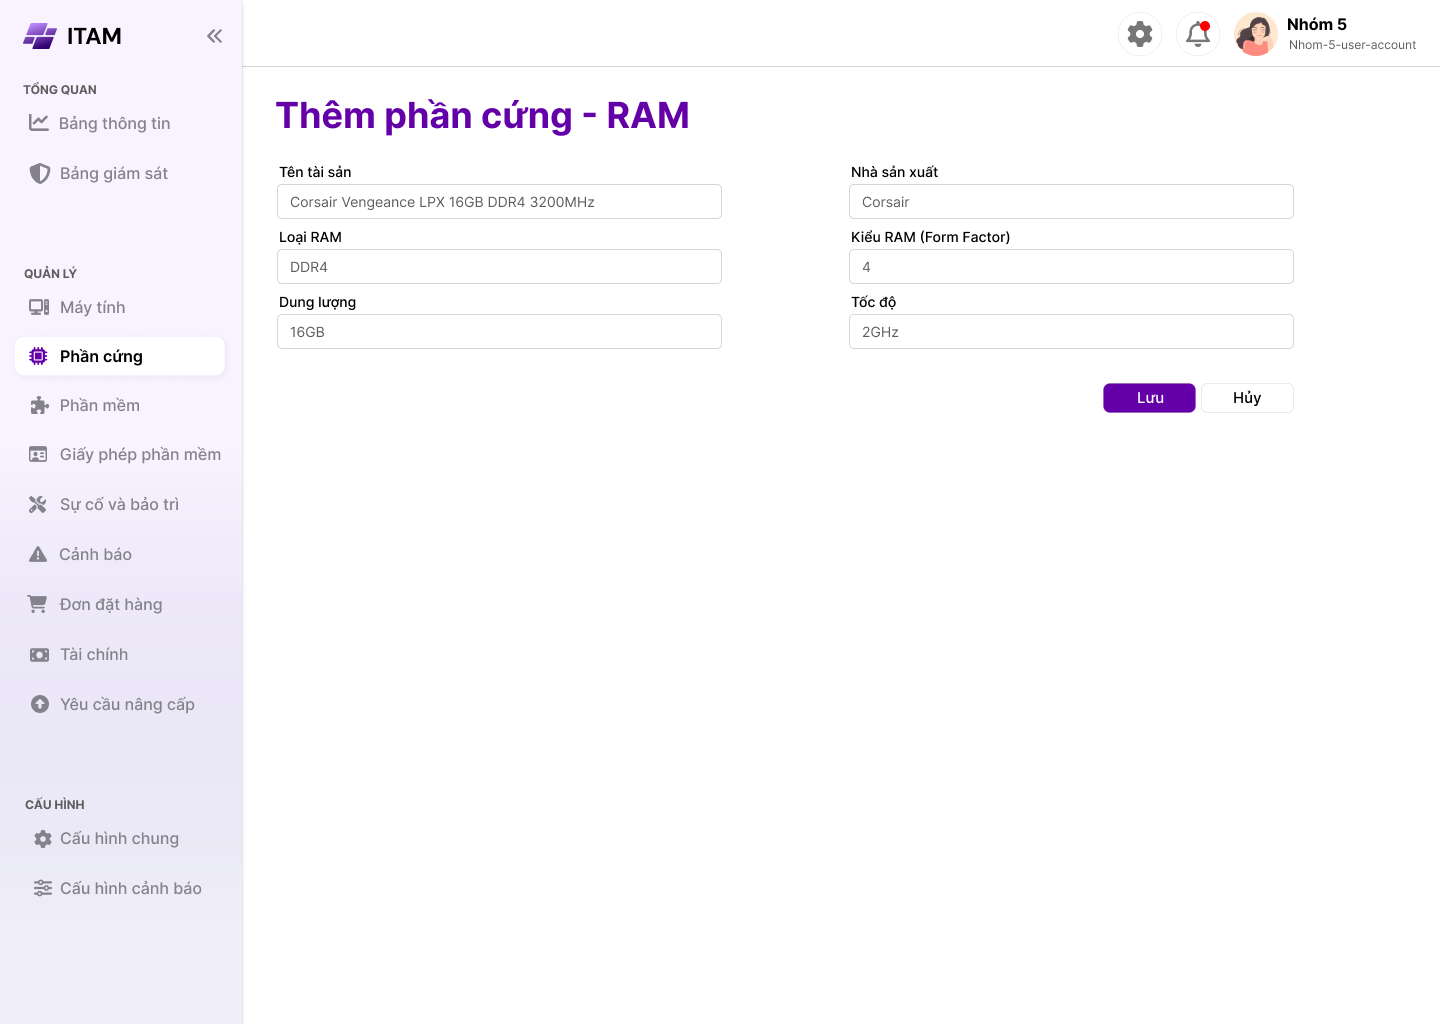
\includegraphics[width=14cm]{Images/C5/UI/Feature-Giám sát tài sản-Phần cứng 4.6.png}
%     \vspace{15pt}
%     \caption{Giao diện Quản lý phần cứng 9}
% \end{figure}
% \begin{figure}[H]
%     \centering
%     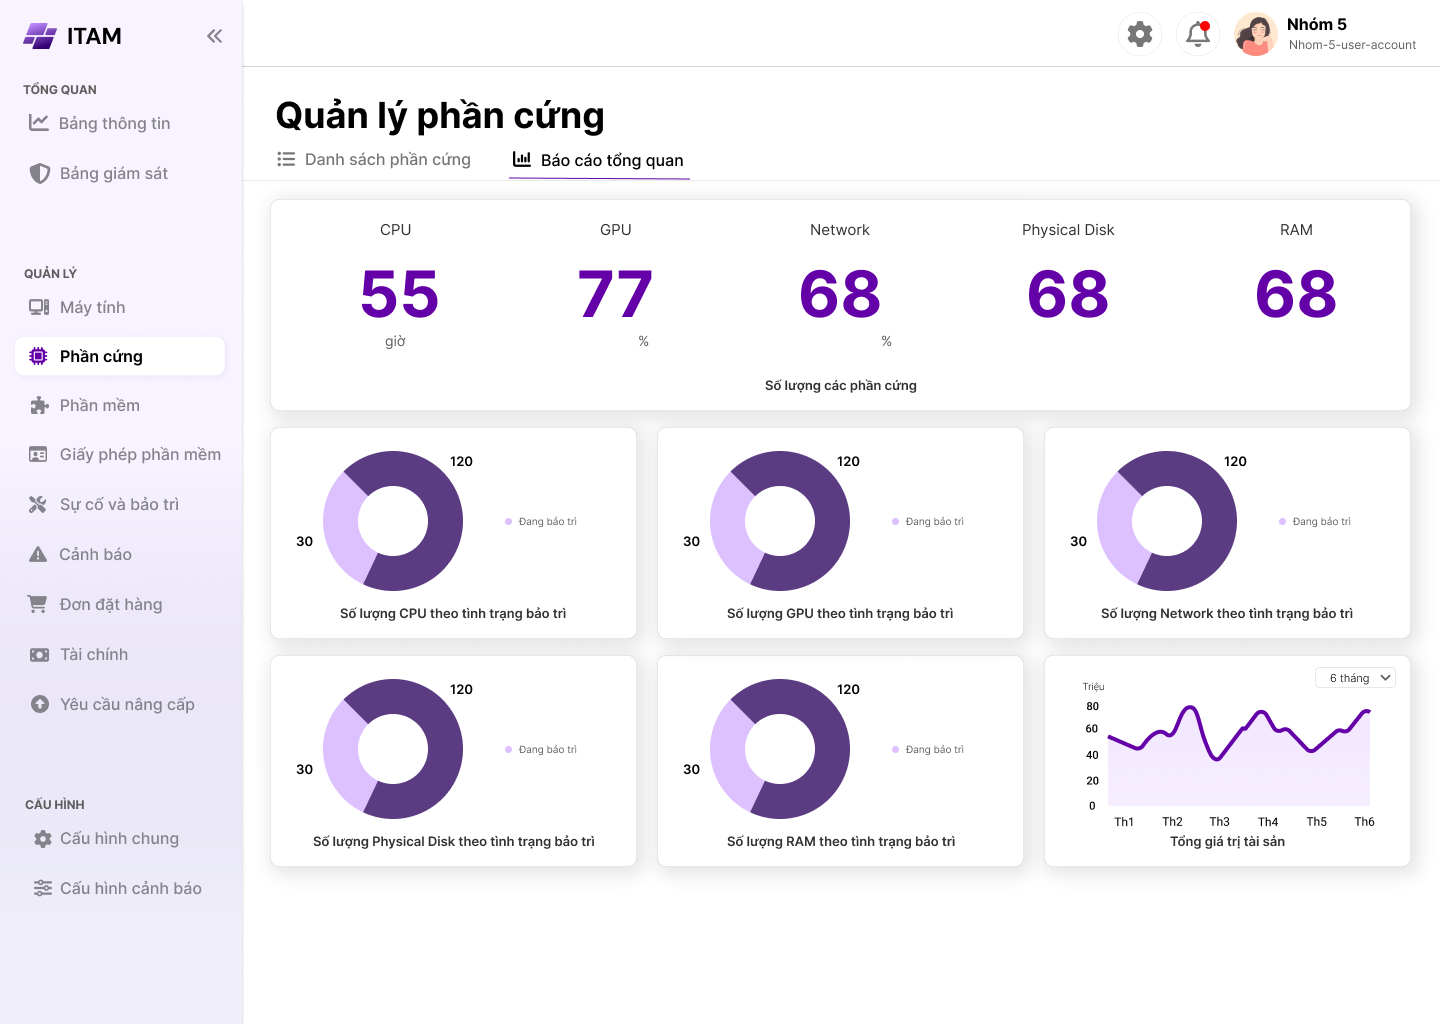
\includegraphics[width=14cm]{Images/C5/UI/Feature-Giám sát tài sản-Phần cứng 3.png}
%     \vspace{15pt}
%     \caption{Giao diện Quản lý phần cứng 4}
% \end{figure}

\item{Quản lý phần mềm}\\
Ở chức năng Quản lý phần mềm, người dùng có thể dễ dàng xem danh sách tất cả các phần mềm trong hệ thống, thêm mới phần mềm, xem chi tiết phần mềm, và xem báo cáo tổng quan về phần mềm (xem thêm chi tiết ở phụ lục).
% \begin{figure}[H]
%     \centering
%     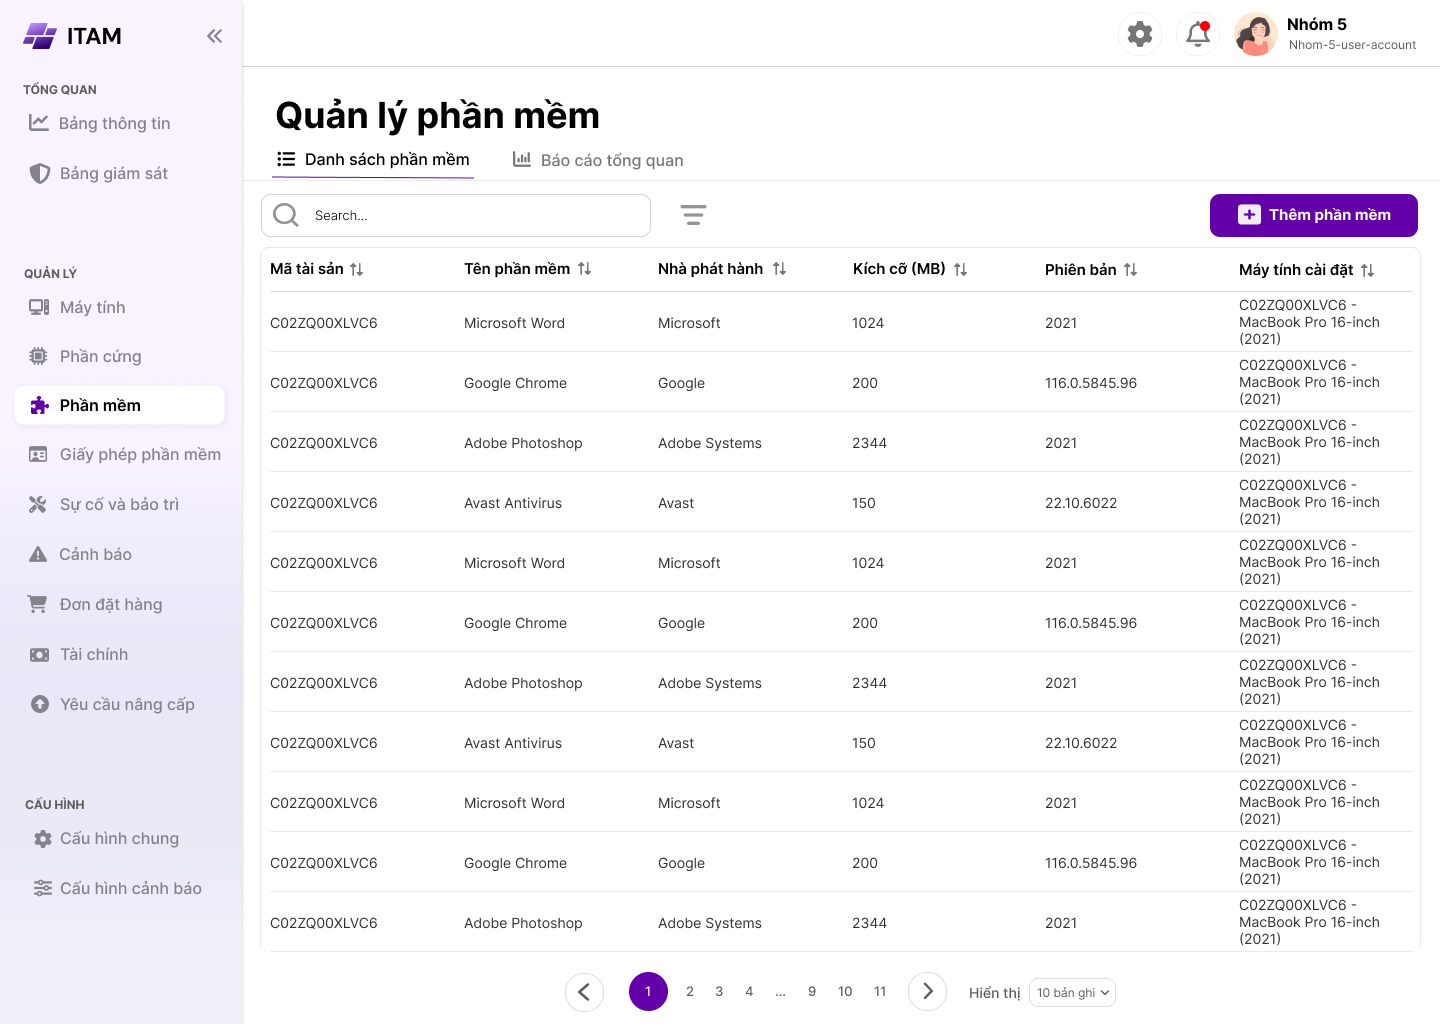
\includegraphics[width=14cm]{Images/C5/UI/Feature-Giám sát tài sản-Phần mềm 1.png}
%     \vspace{15pt}
%     \caption{Giao diện Quản lý phần mềm 1}
% \end{figure}
% \begin{figure}[H]
%     \centering
%     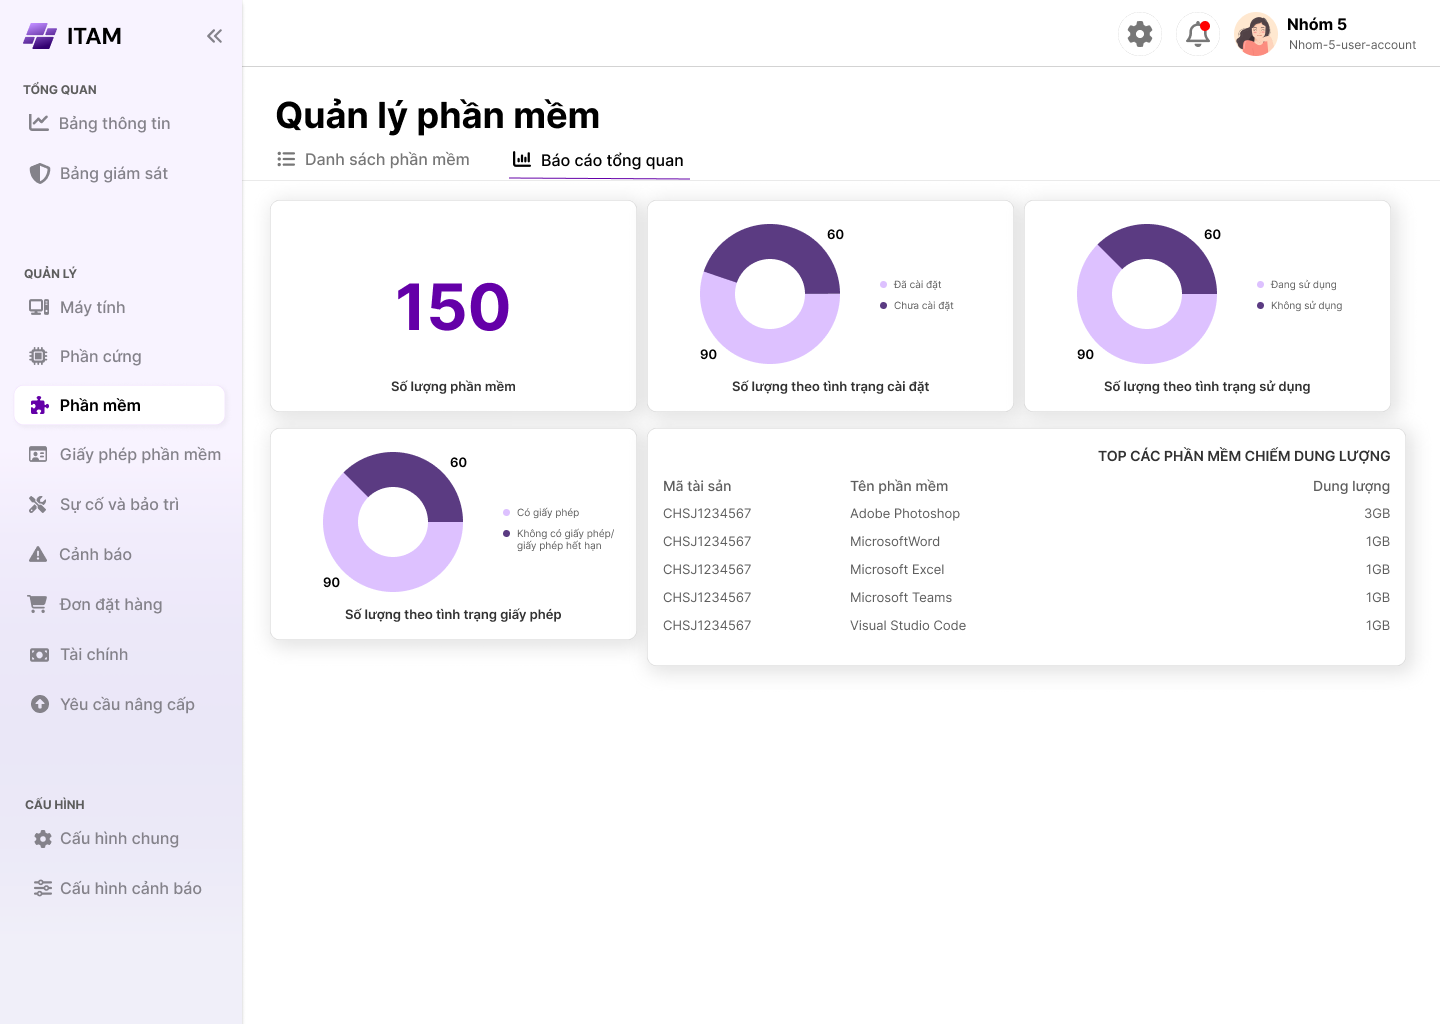
\includegraphics[width=14cm]{Images/C5/UI/Feature-Giám sát tài sản-Phần mềm 2.png}
%     \vspace{15pt}
%     \caption{Giao diện Quản lý phần mềm 2}
% \end{figure}
% \begin{figure}[H]
%     \centering
%     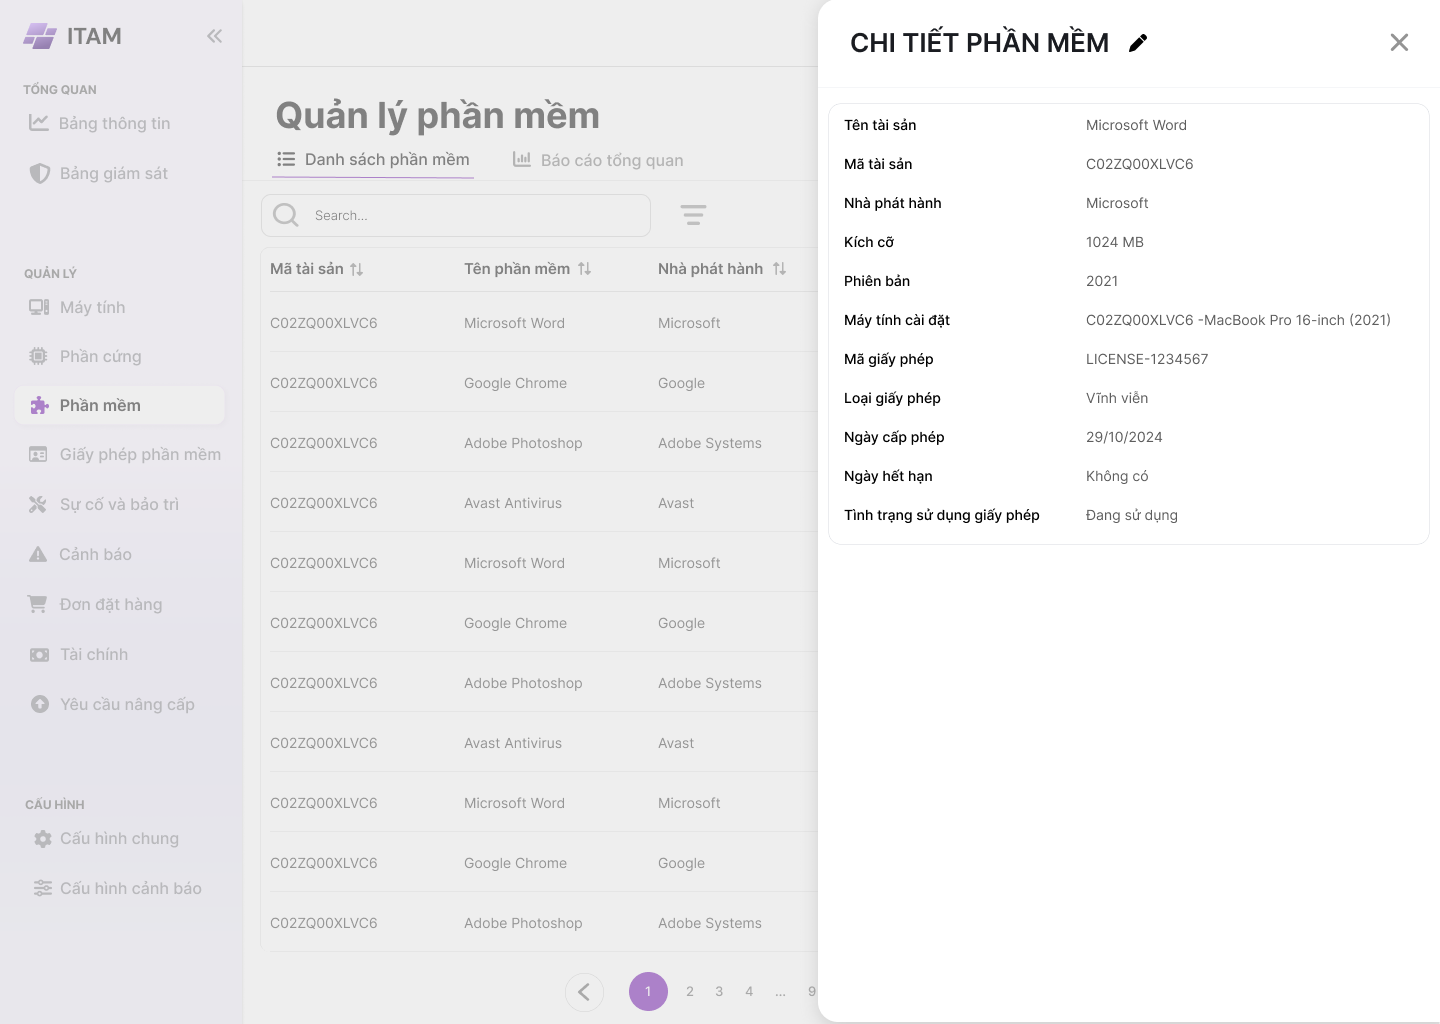
\includegraphics[width=14cm]{Images/C5/UI/Feature-Giám sát tài sản-Phần mềm 3.png}
%     \vspace{15pt}
%     \caption{Giao diện Quản lý phần mềm 3}
% \end{figure}
% \begin{figure}[H]
%     \centering
%     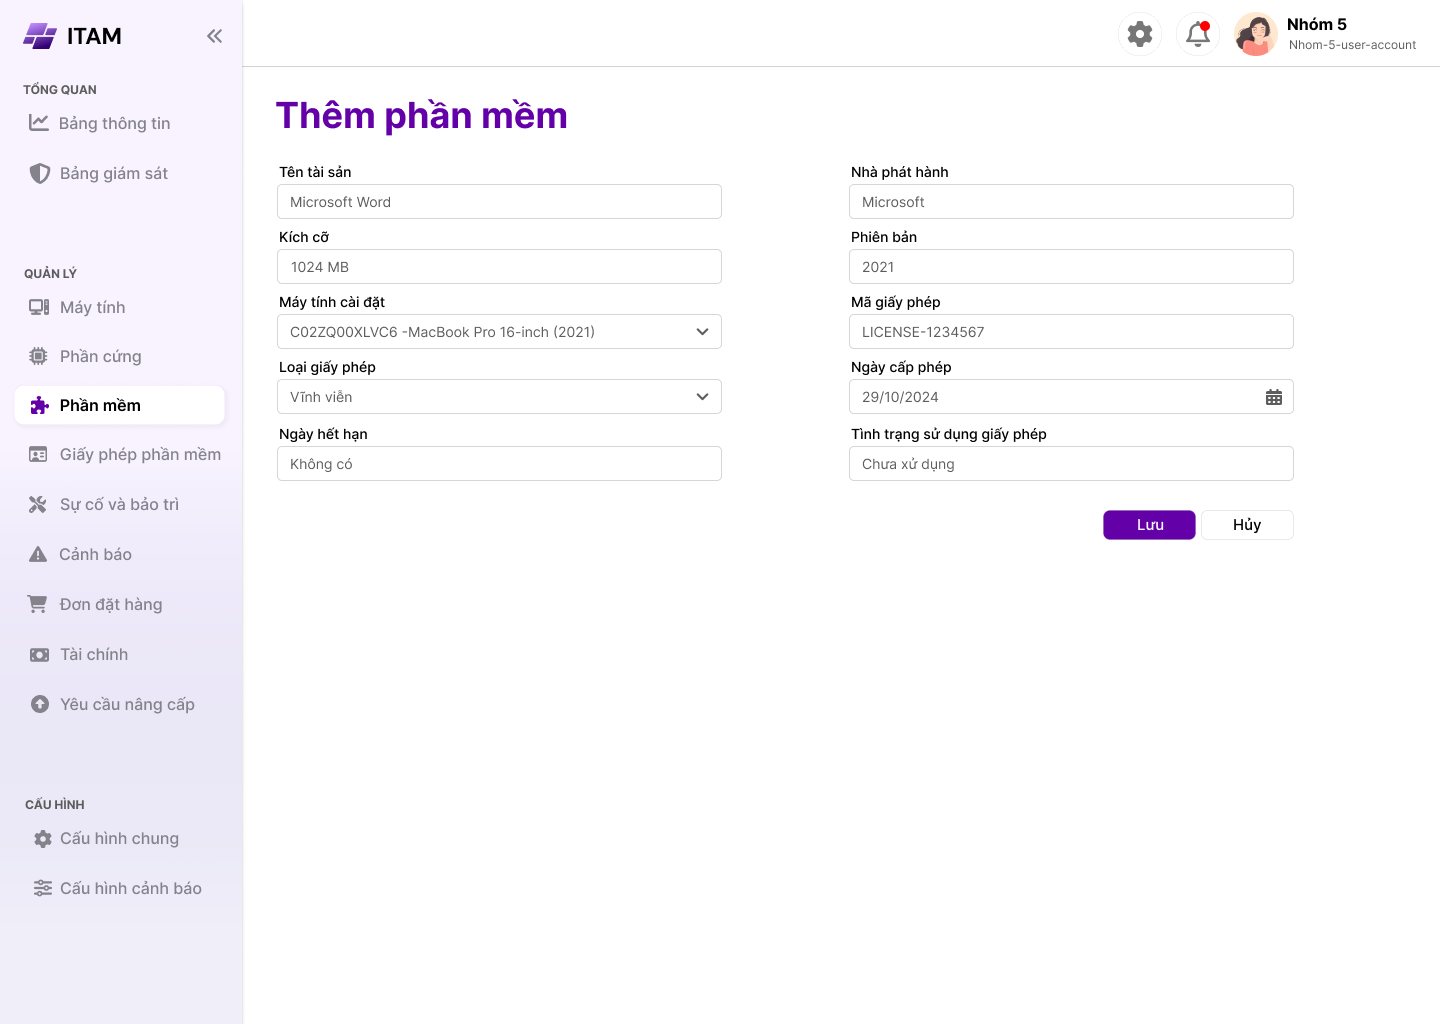
\includegraphics[width=14cm]{Images/C5/UI/Feature-Giám sát tài sản-Phần mềm 4.png}
%     \vspace{15pt}
%     \caption{Giao diện Quản lý phần mềm 4}
% \end{figure}

\item{Quản lý sự cố và bảo trì}\\
Quản lý sự cố và bảo trì cung cấp các tính năng xem danh sách, chi tiết sự cố và yêu cầu bảo trì của tài sản, giúp người dùng có thể quản lý một cách tập trung sự cố và bảo trì trong hệ thống (xem thêm chi tiết ở phụ lục).
% \begin{figure}[H]
%     \centering
%     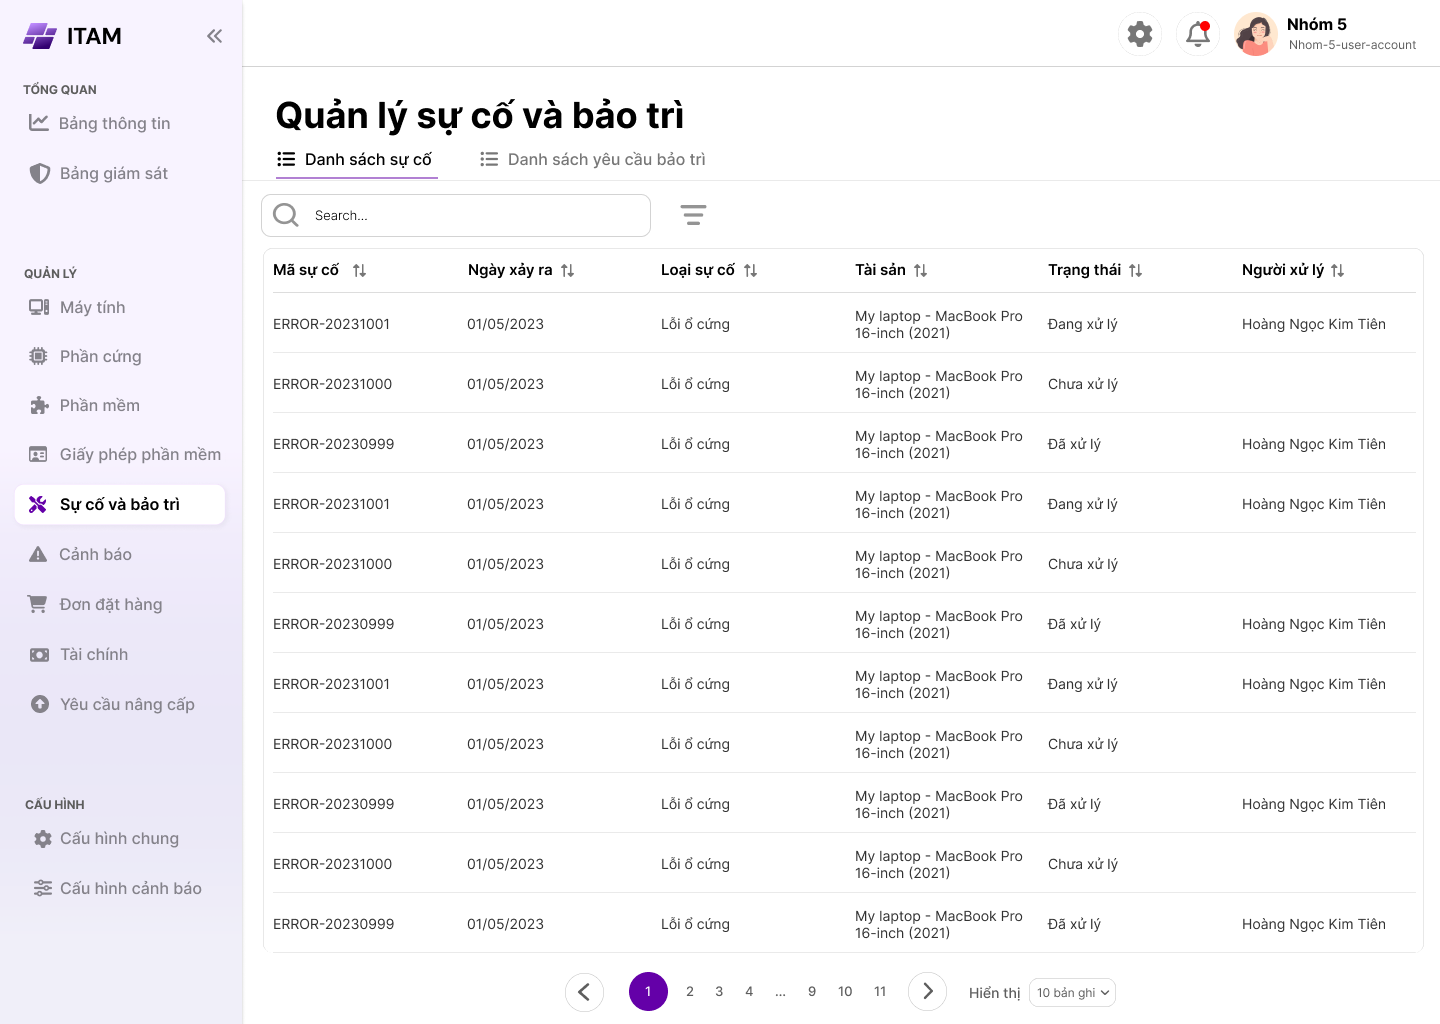
\includegraphics[width=14cm]{Images/C5/UI/Feature-Quản lý sự cố và bảo trì 1.png}
%     \vspace{15pt}
%     \caption{Giao diện Quản lý sự cố và bảo trì 1}
% \end{figure}
% \begin{figure}[H]
%     \centering
%     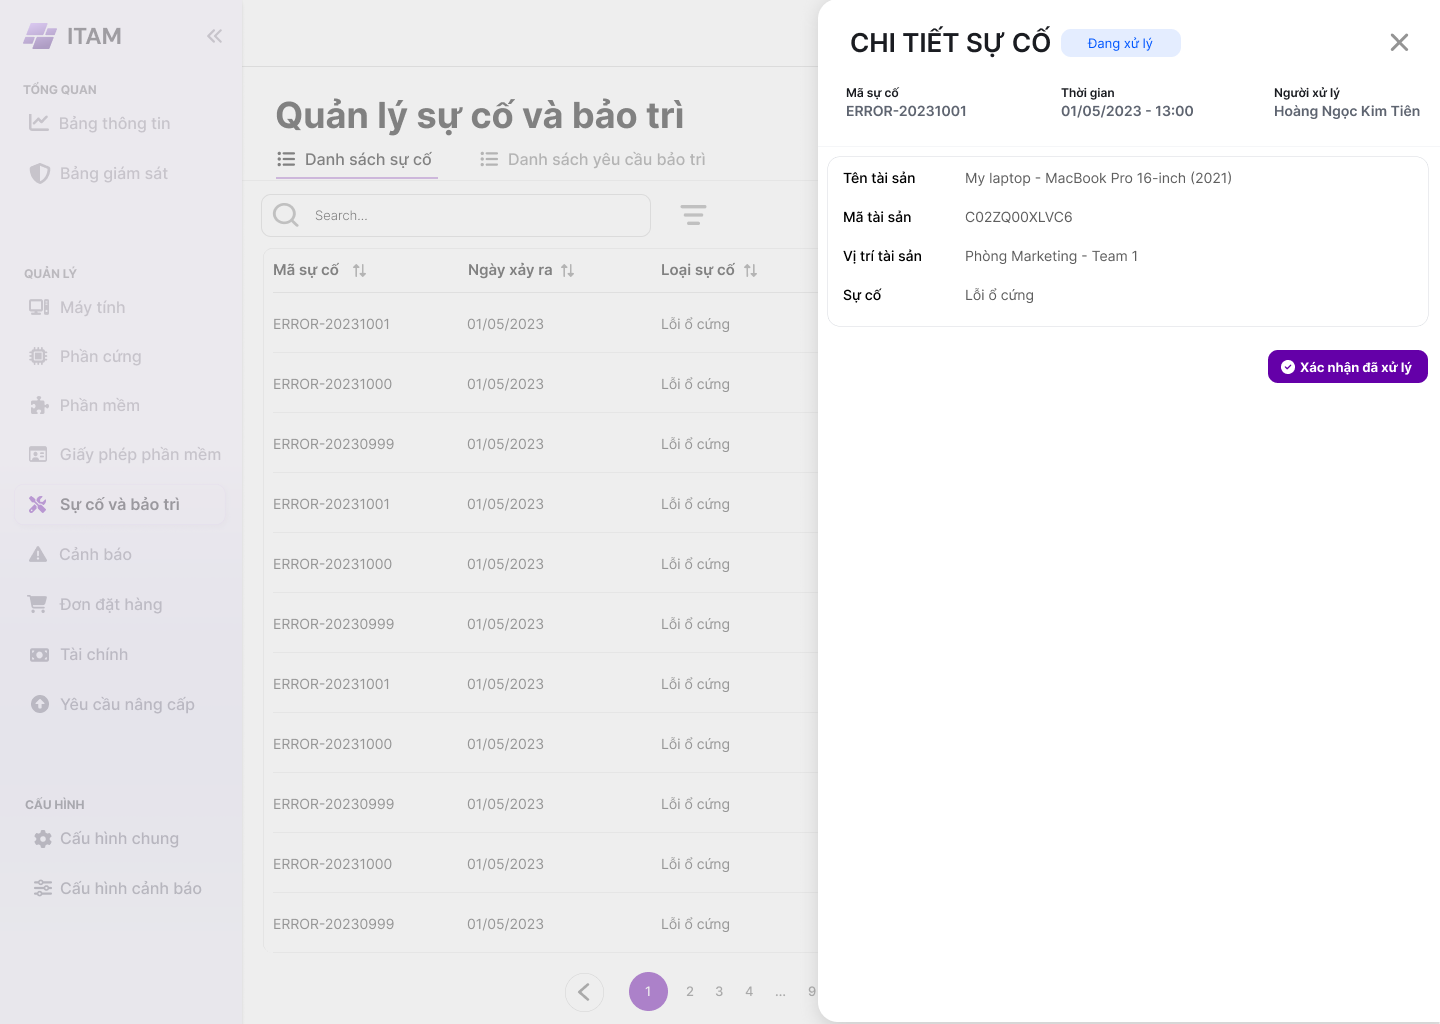
\includegraphics[width=14cm]{Images/C5/UI/Feature-Quản lý sự cố và bảo trì 2.1.png}
%     \vspace{15pt}
%     \caption{Giao diện Quản lý sự cố và bảo trì 2}
% \end{figure}
% \begin{figure}[H]
%     \centering
%     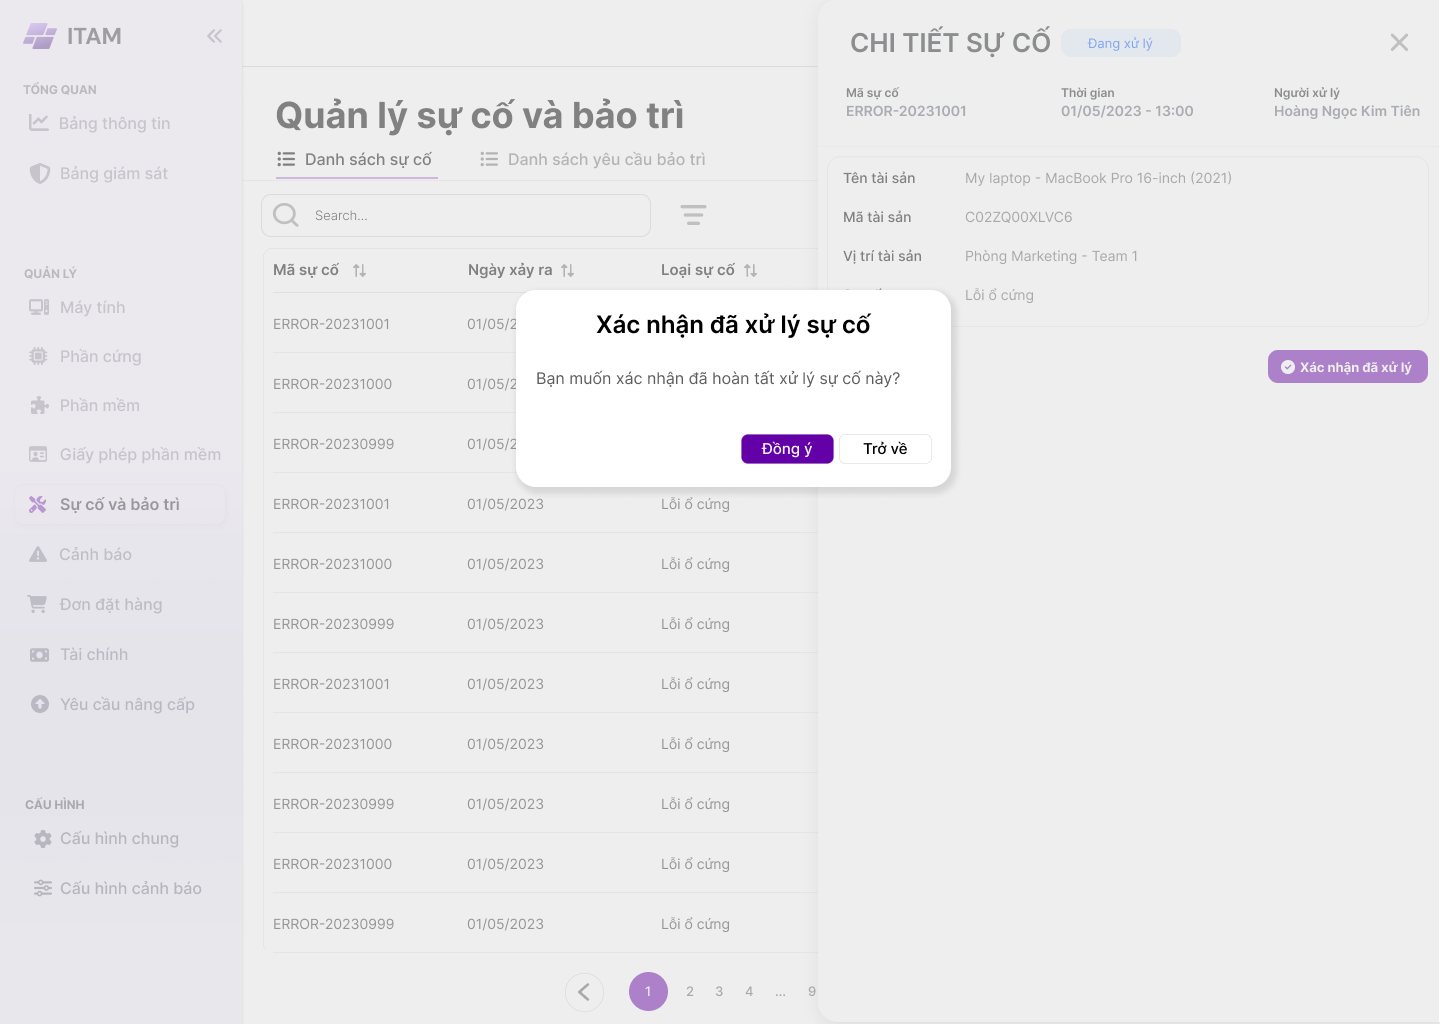
\includegraphics[width=14cm]{Images/C5/UI/Feature-Quản lý sự cố và bảo trì 2.2.png}
%     \vspace{15pt}
%     \caption{Giao diện Quản lý sự cố và bảo trì 3}
% \end{figure}
% \begin{figure}[H]
%     \centering
%     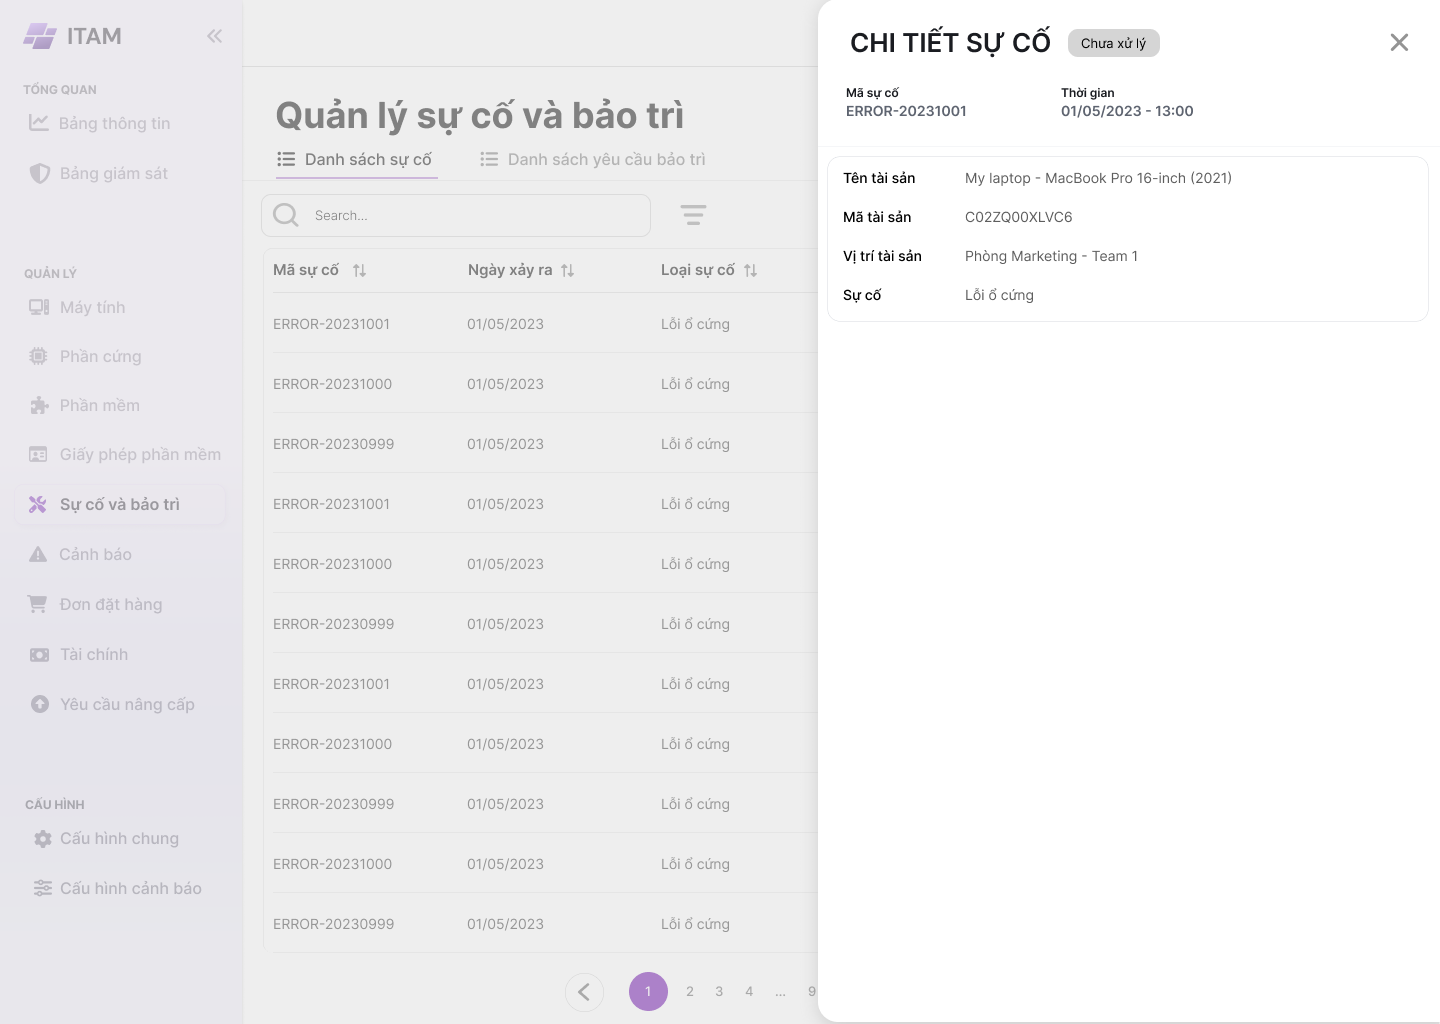
\includegraphics[width=14cm]{Images/C5/UI/Feature-Quản lý sự cố và bảo trì 2.3.png}
%     \vspace{15pt}
%     \caption{Giao diện Quản lý sự cố và bảo trì 4}
% \end{figure}
% \begin{figure}[H]
%     \centering
%     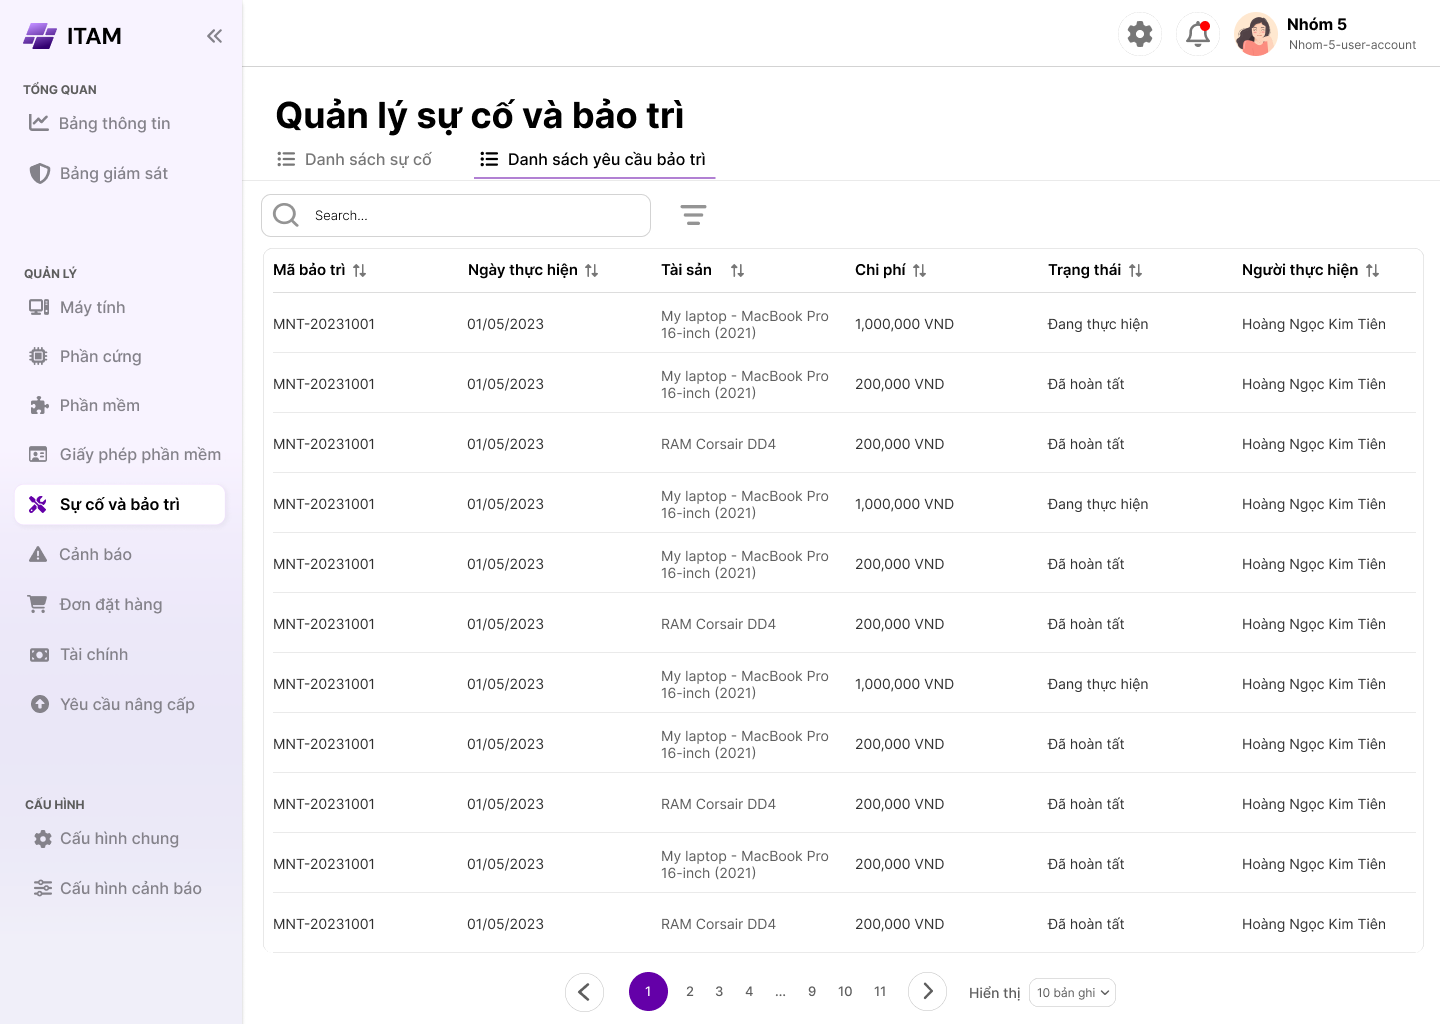
\includegraphics[width=14cm]{Images/C5/UI/Feature-Quản lý sự cố và bảo trì 3.1.png}
%     \vspace{15pt}
%     \caption{Giao diện Quản lý sự cố và bảo trì 3}
% \end{figure}
% \begin{figure}[H]
%     \centering
%     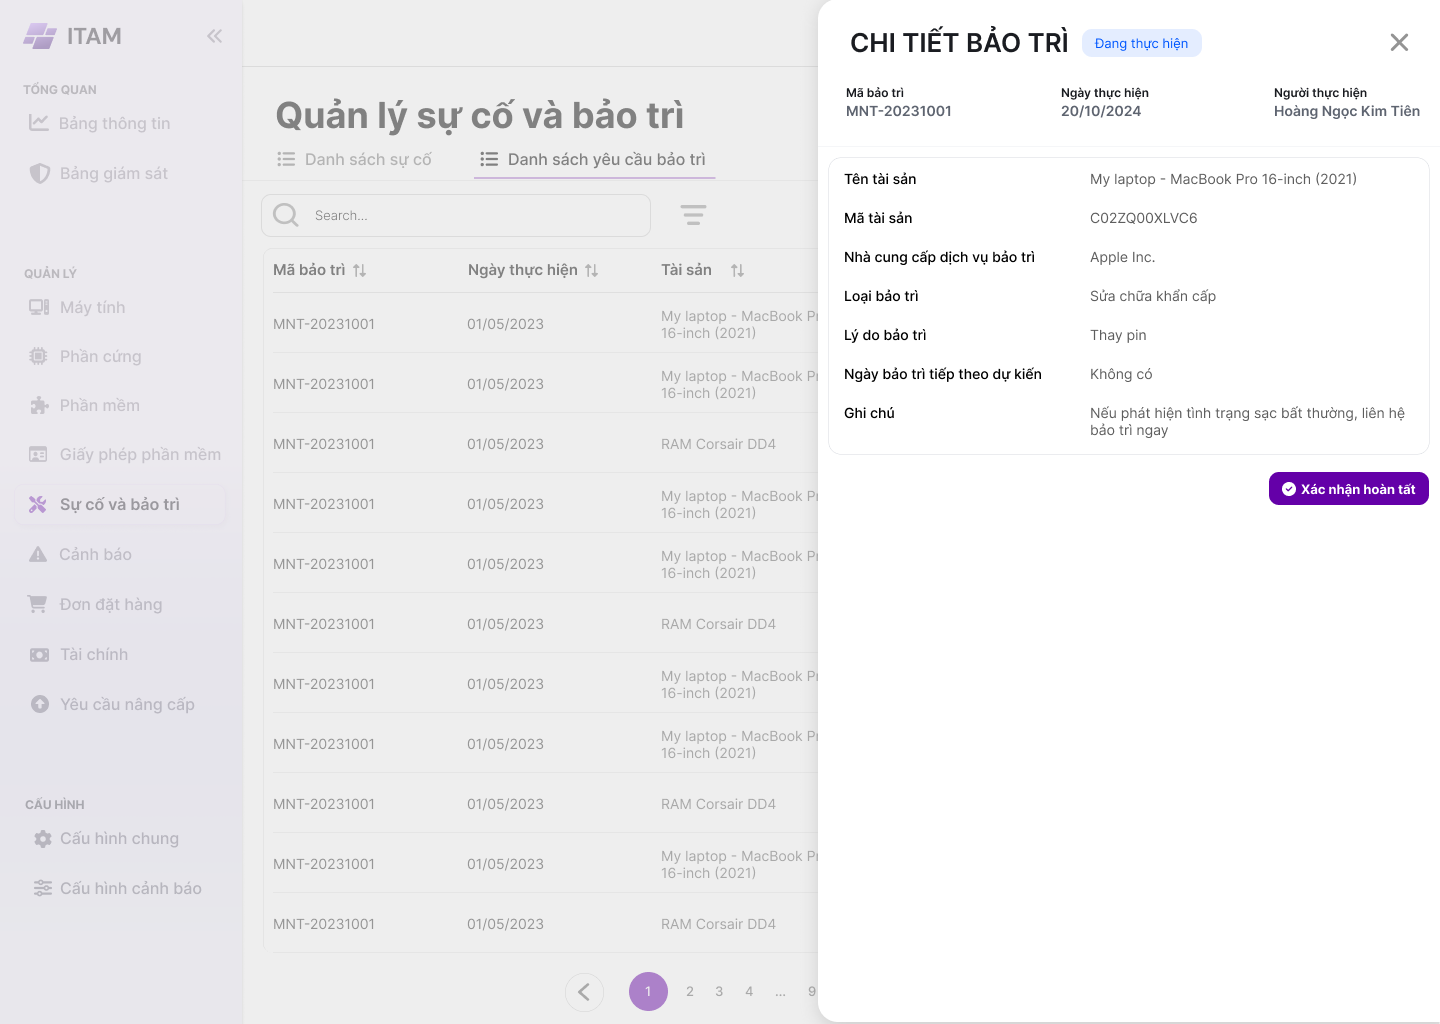
\includegraphics[width=14cm]{Images/C5/UI/Feature-Quản lý sự cố và bảo trì 3.2.png}
%     \vspace{15pt}
%     \caption{Giao diện Quản lý sự cố và bảo trì 4}
% \end{figure}
% \begin{figure}[H]
%     \centering
%     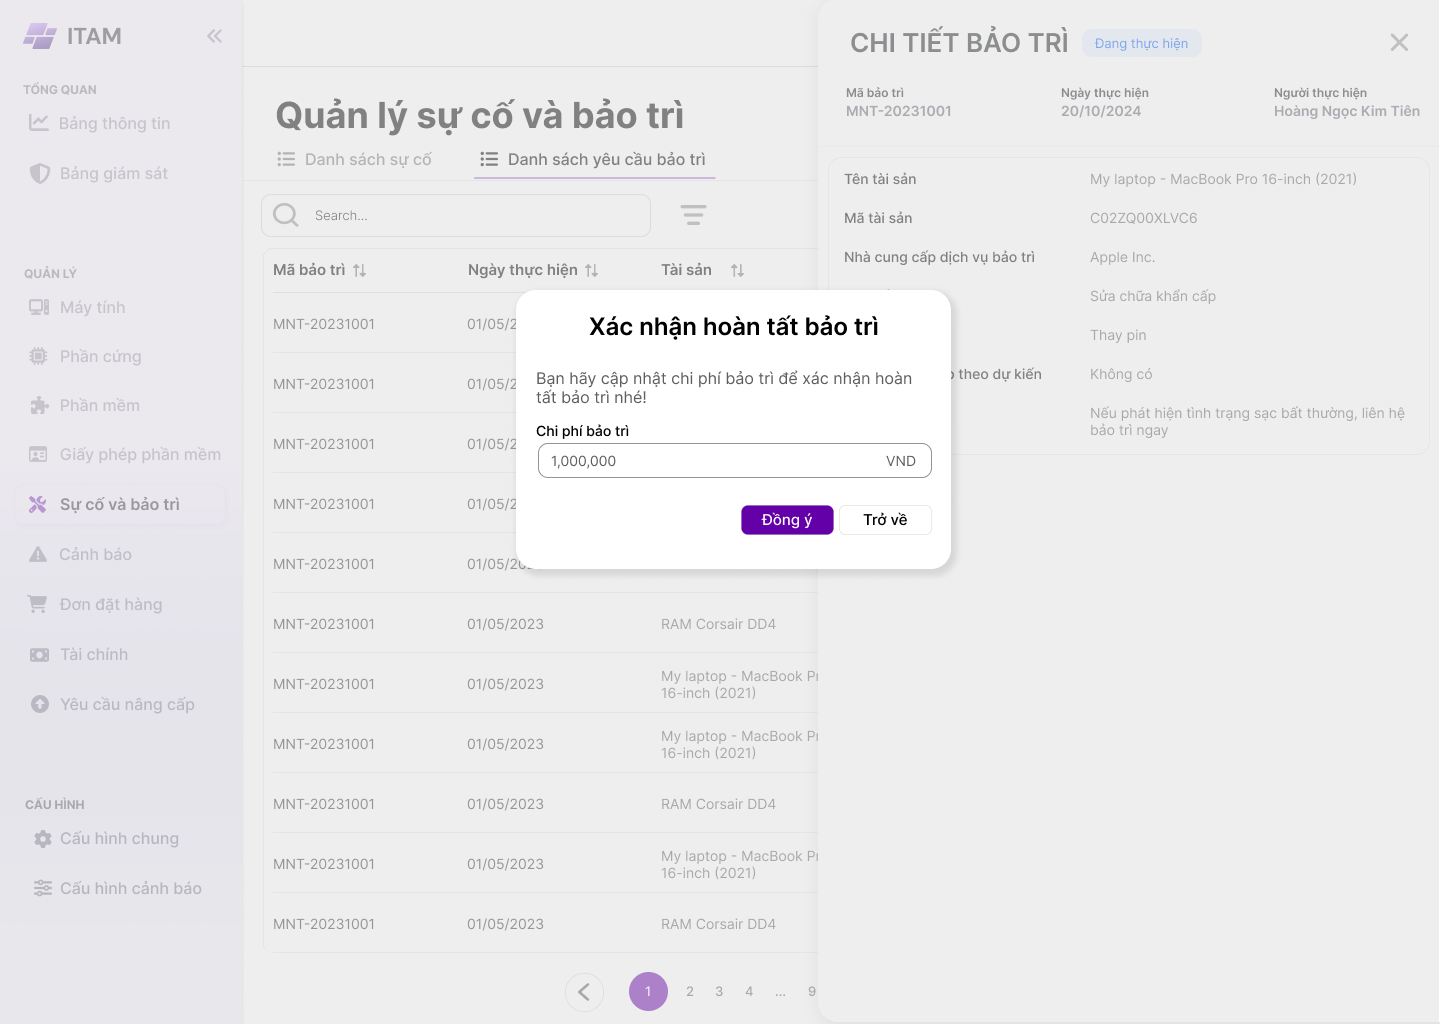
\includegraphics[width=14cm]{Images/C5/UI/Feature-Quản lý sự cố và bảo trì 3.3.png}
%     \vspace{15pt}
%     \caption{Giao diện Quản lý sự cố và bảo trì 7}
% \end{figure}

\item{Quản lý cảnh báo}\\
Ở Quản lý cảnh báo, người cùng có thể xem tất cả các cảnh báo của các máy tính có trong hệ thống và xem chi tiết các cảnh báo đó. Cảnh báo cũng được phân loại màu sắc dựa trên mức độ nghiêm trọng để người dùng có thể kịp thời đưa ra quyết định xử lý các cảnh báo quan trọng (xem thêm chi tiết ở phụ lục).
% \begin{figure}[H]
%     \centering
%     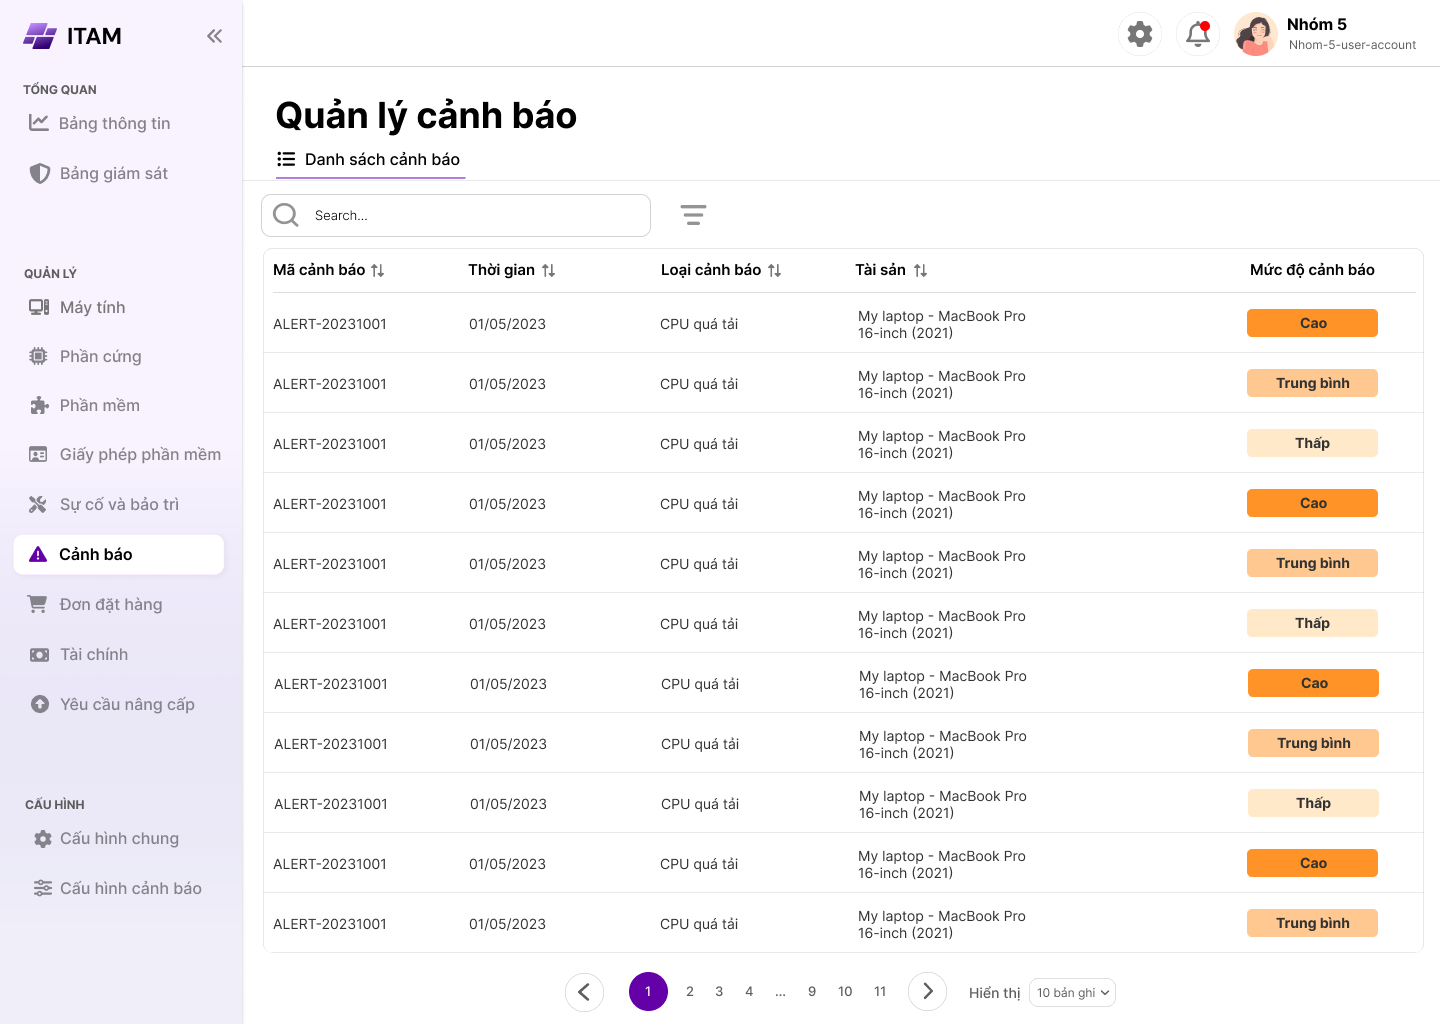
\includegraphics[width=14cm]{Images/C5/UI/Feature-Quản lý cảnh báo 1.png}
%     \vspace{15pt}
%     \caption{Giao diện Quản lý cảnh báo 1}
% \end{figure}
% \begin{figure}[H]
%     \centering
%     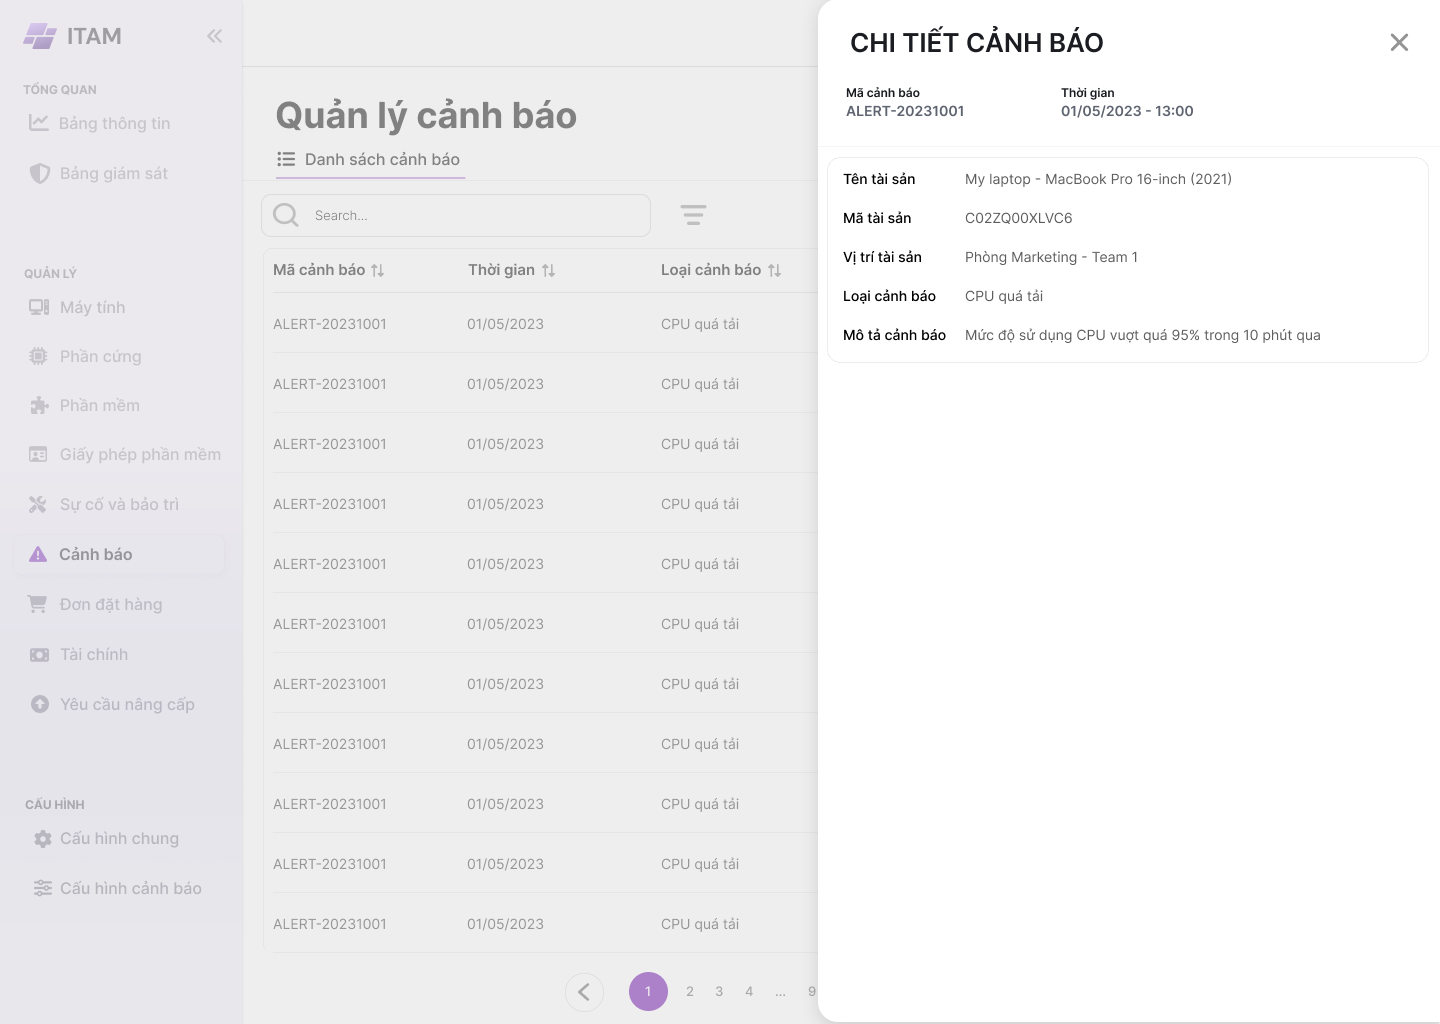
\includegraphics[width=14cm]{Images/C5/UI/Feature-Quản lý cảnh báo 2.1.png}
%     \vspace{15pt}
%     \caption{Giao diện Quản lý cảnh báo 2}
% \end{figure}

\item{Quản lý yêu cầu nâng cấp}\\
Người dùng có thể xem danh sách các yêu cầu nâng cấp và chi tiết các yêu cầu nâng cấp đó, đồng thời quản lý cũng có thể phê duyệt các yêu cầu nâng cấp (xem thêm chi tiết ở phụ lục).
% \begin{figure}[H]
%     \centering
%     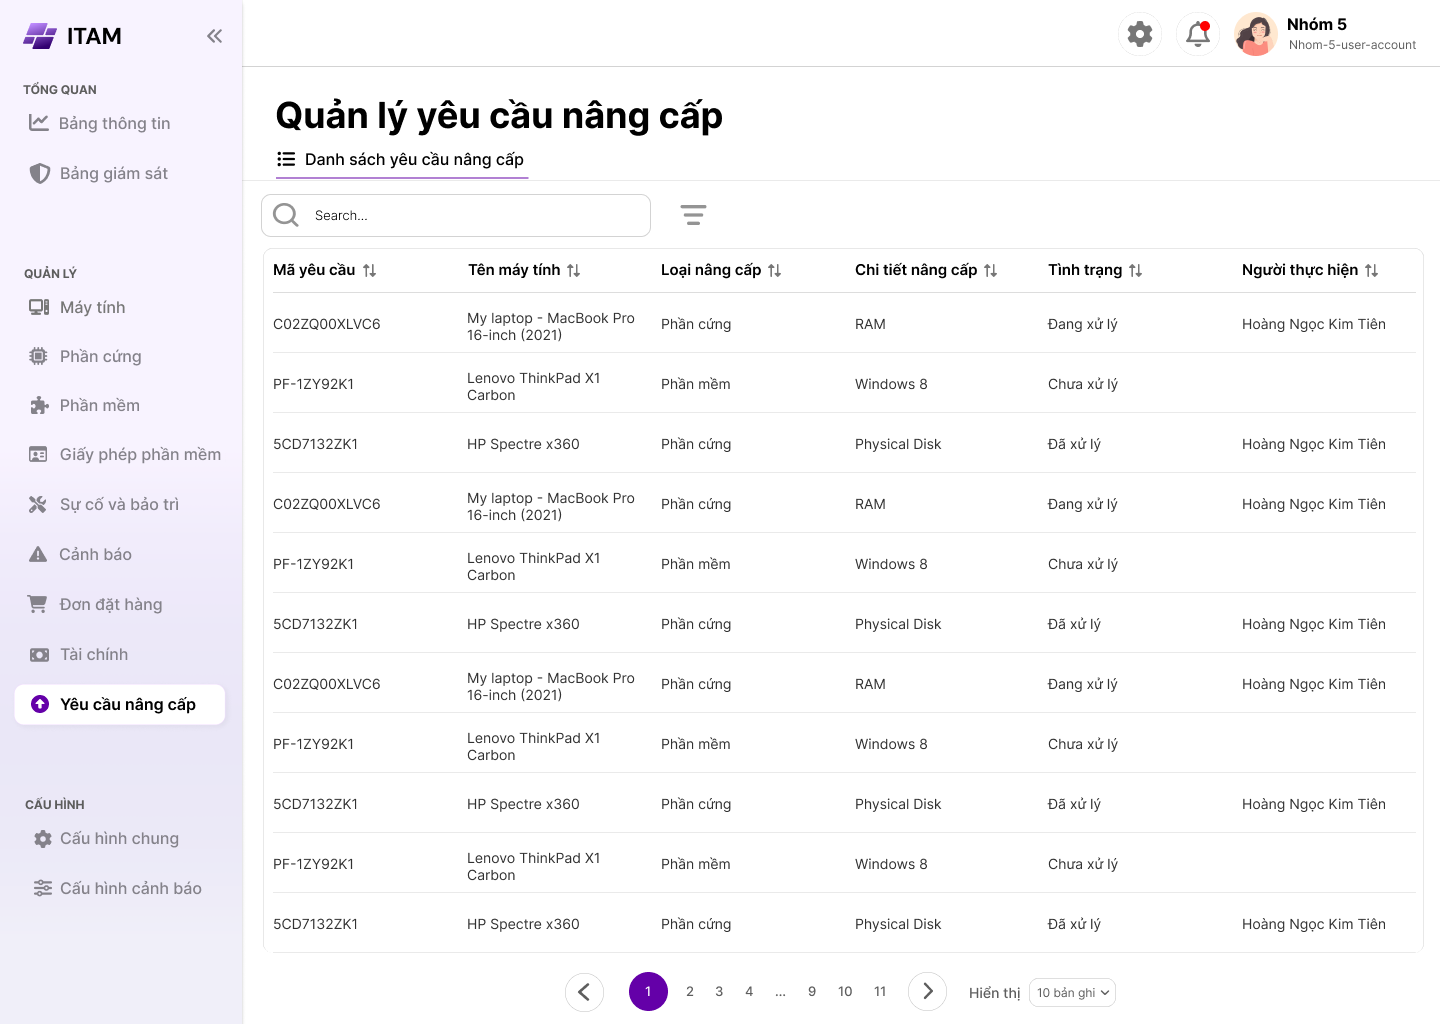
\includegraphics[width=14cm]{Images/C5/UI/Feature-Quản lý yêu cầu nâng cấp 1.png}
%     \vspace{15pt}
%     \caption{Giao diện Quản lý yêu cầu nâng cấp 1}
% \end{figure}
% \begin{figure}[H]
%     \centering
%     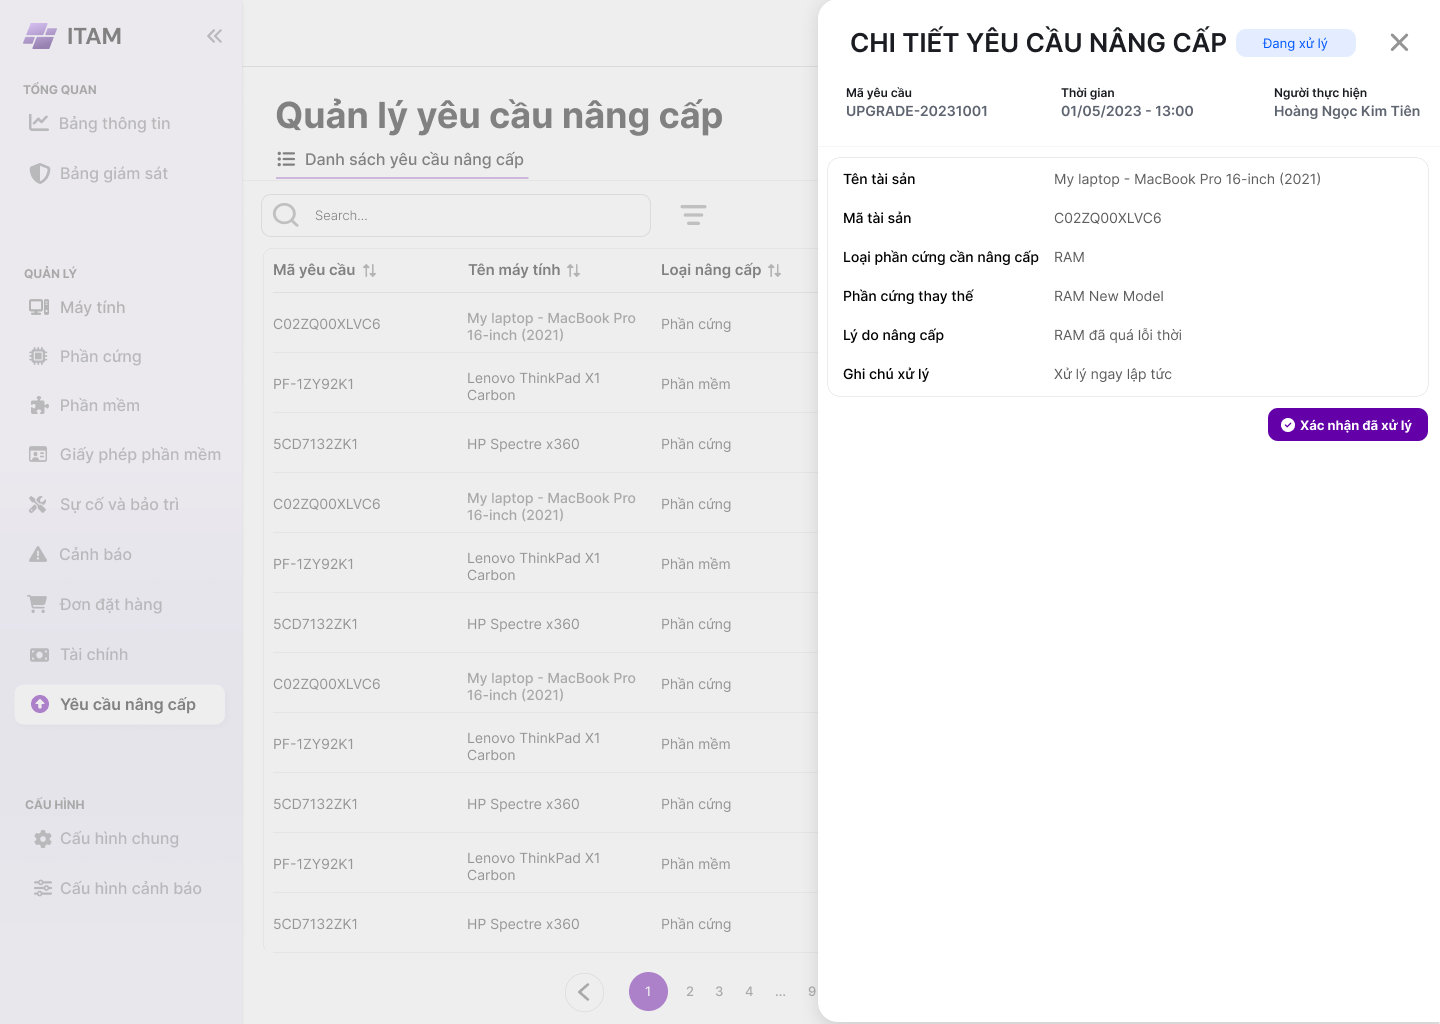
\includegraphics[width=14cm]{Images/C5/UI/Feature-Quản lý yêu cầu nâng cấp 2.1.png}
%     \vspace{15pt}
%     \caption{Giao diện Quản lý yêu cầu nâng cấp 2}
% \end{figure}
% \begin{figure}[H]
%     \centering
%     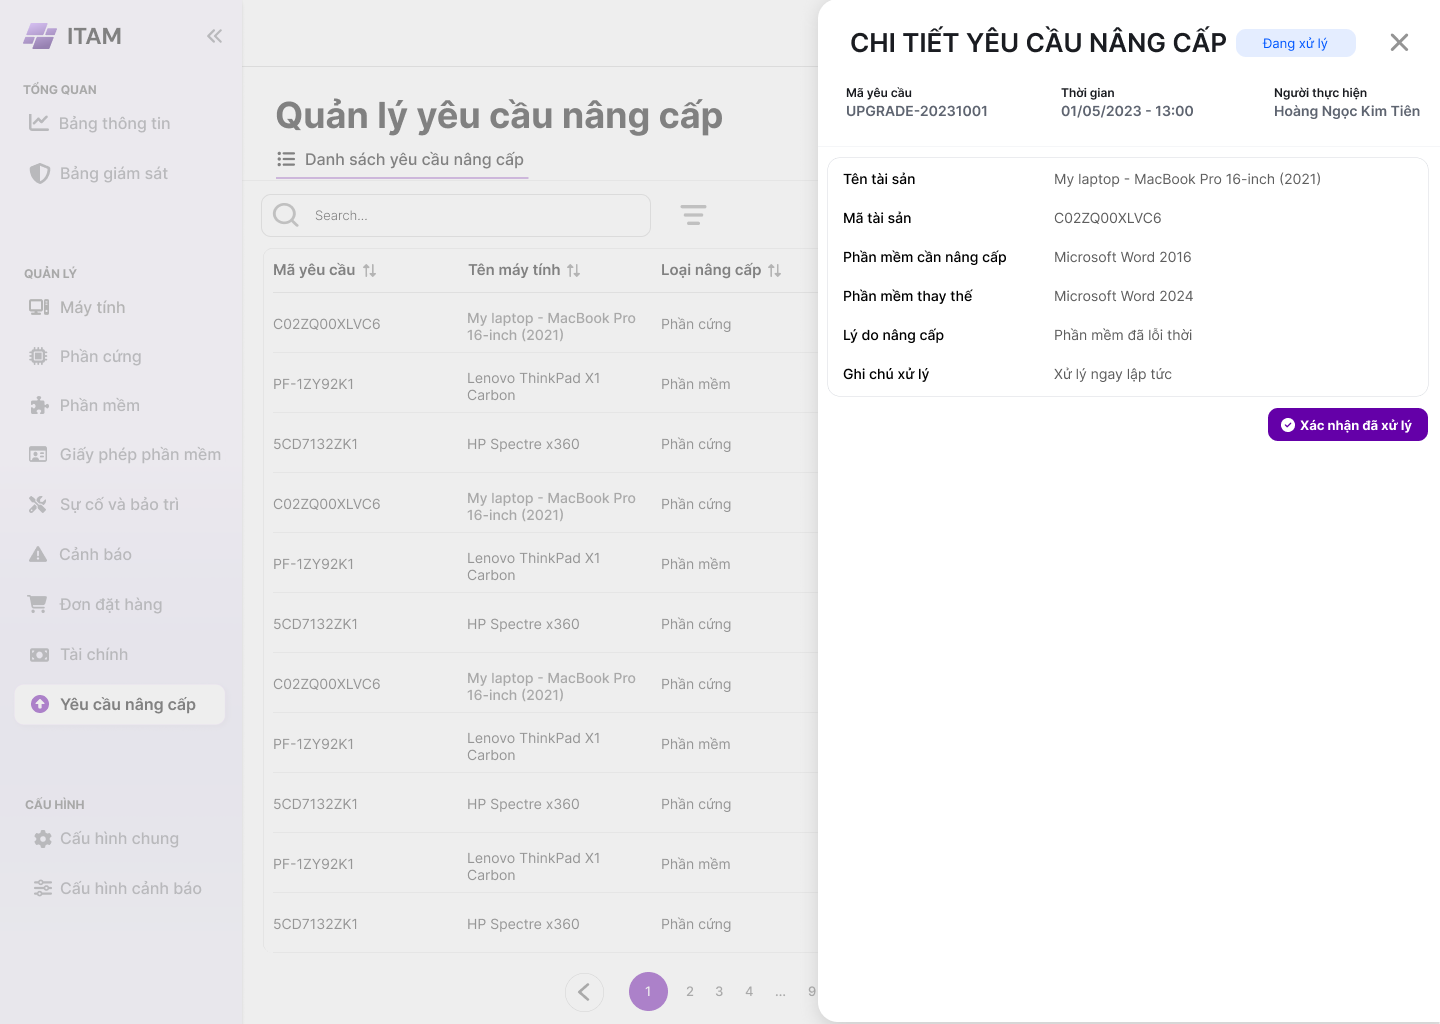
\includegraphics[width=14cm]{Images/C5/UI/Feature-Quản lý yêu cầu nâng cấp 2.2.png}
%     \vspace{15pt}
%     \caption{Giao diện Quản lý yêu cầu nâng cấp 3}
% \end{figure}
% \begin{figure}[H]
%     \centering
%     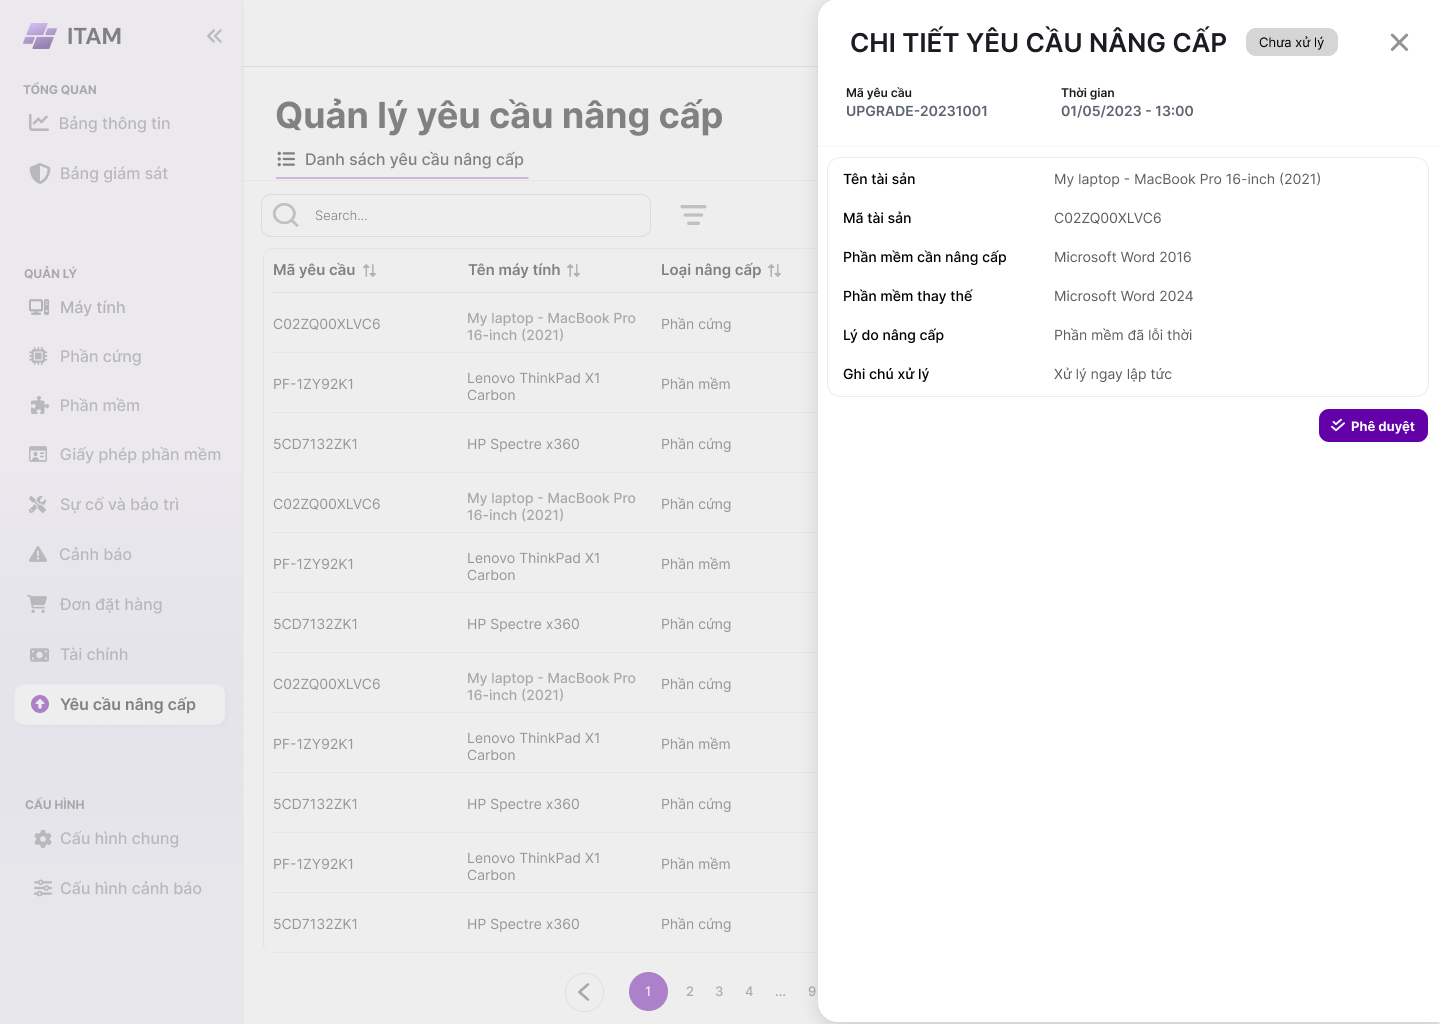
\includegraphics[width=14cm]{Images/C5/UI/Feature-Quản lý yêu cầu nâng cấp 2.3.png}
%     \vspace{15pt}
%     \caption{Giao diện Quản lý yêu cầu nâng cấp 2}
% \end{figure}
% \begin{figure}[H]
%     \centering
%     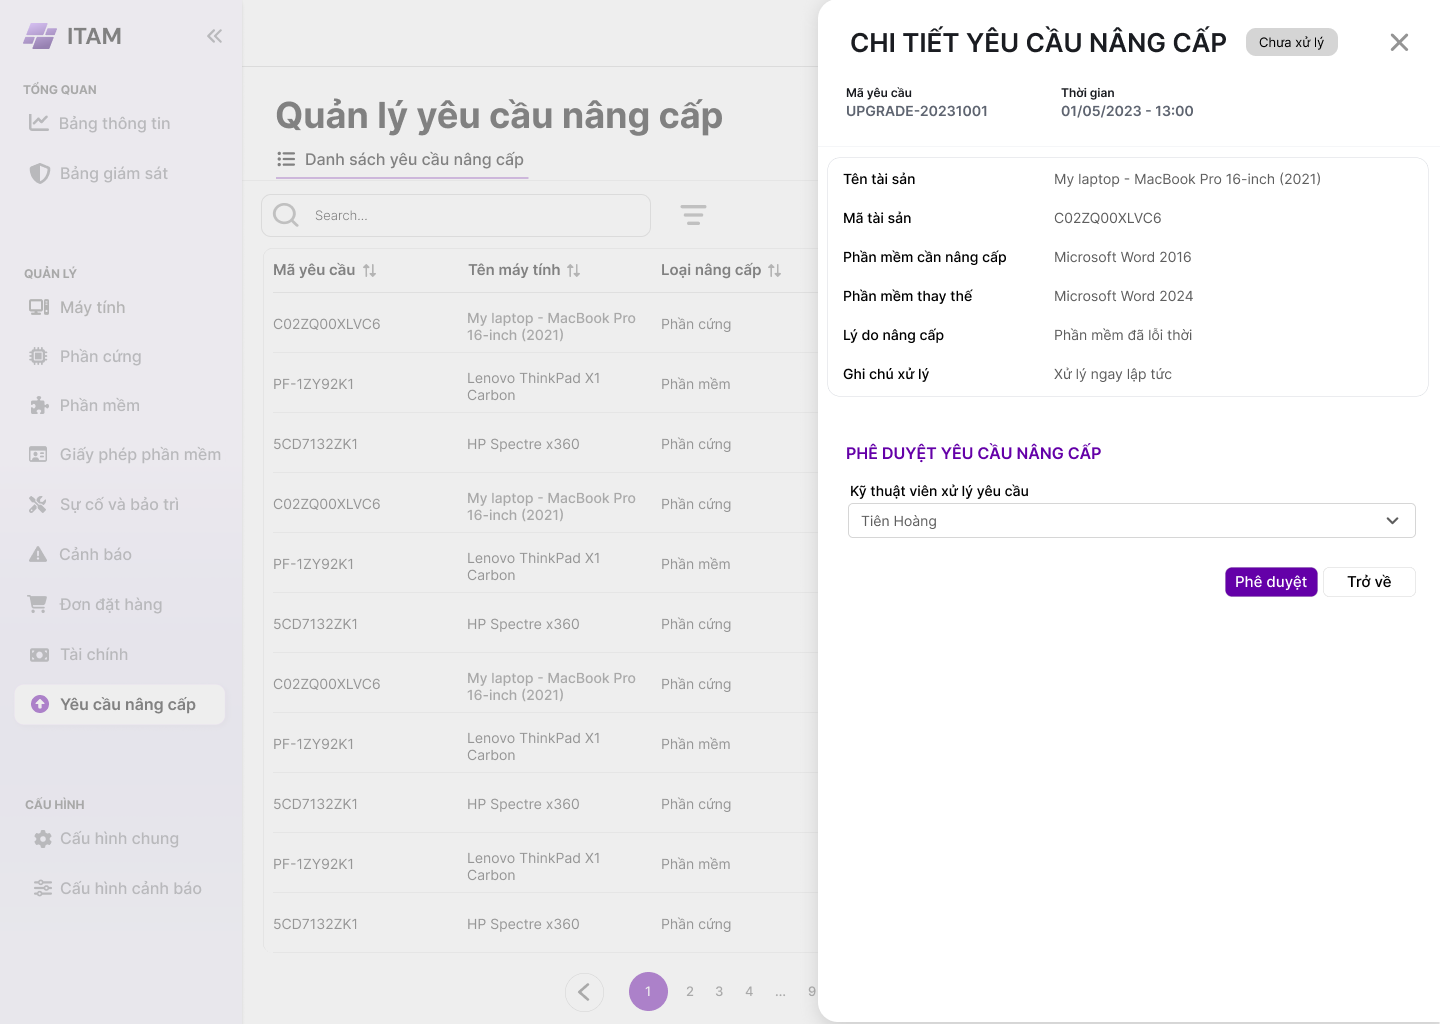
\includegraphics[width=14cm]{Images/C5/UI/Feature-Quản lý yêu cầu nâng cấp 2.4.png}
%     \vspace{15pt}
%     \caption{Giao diện Quản lý yêu cầu nâng cấp 2}
% \end{figure}

\item{Quản lý yêu cầu thanh lý}\\
Người dùng có thể xem danh sách các yêu cầu thanh lý và chi tiết các yêu cầu thanh lý đó, đồng thời quản lý cũng có thể phê duyệt các yêu cầu thanh lý (xem thêm chi tiết ở phụ lục).

\item{Quản lý đơn đặt hàng}\\
Người dùng với vai trò quản lý có thể xem danh sách đơn đặt hàng và chi tiết đơn đặt hàng, tạo đơn đặt hàng mới (xem thêm chi tiết ở phụ lục).
% \begin{figure}[H]
%     \centering
%     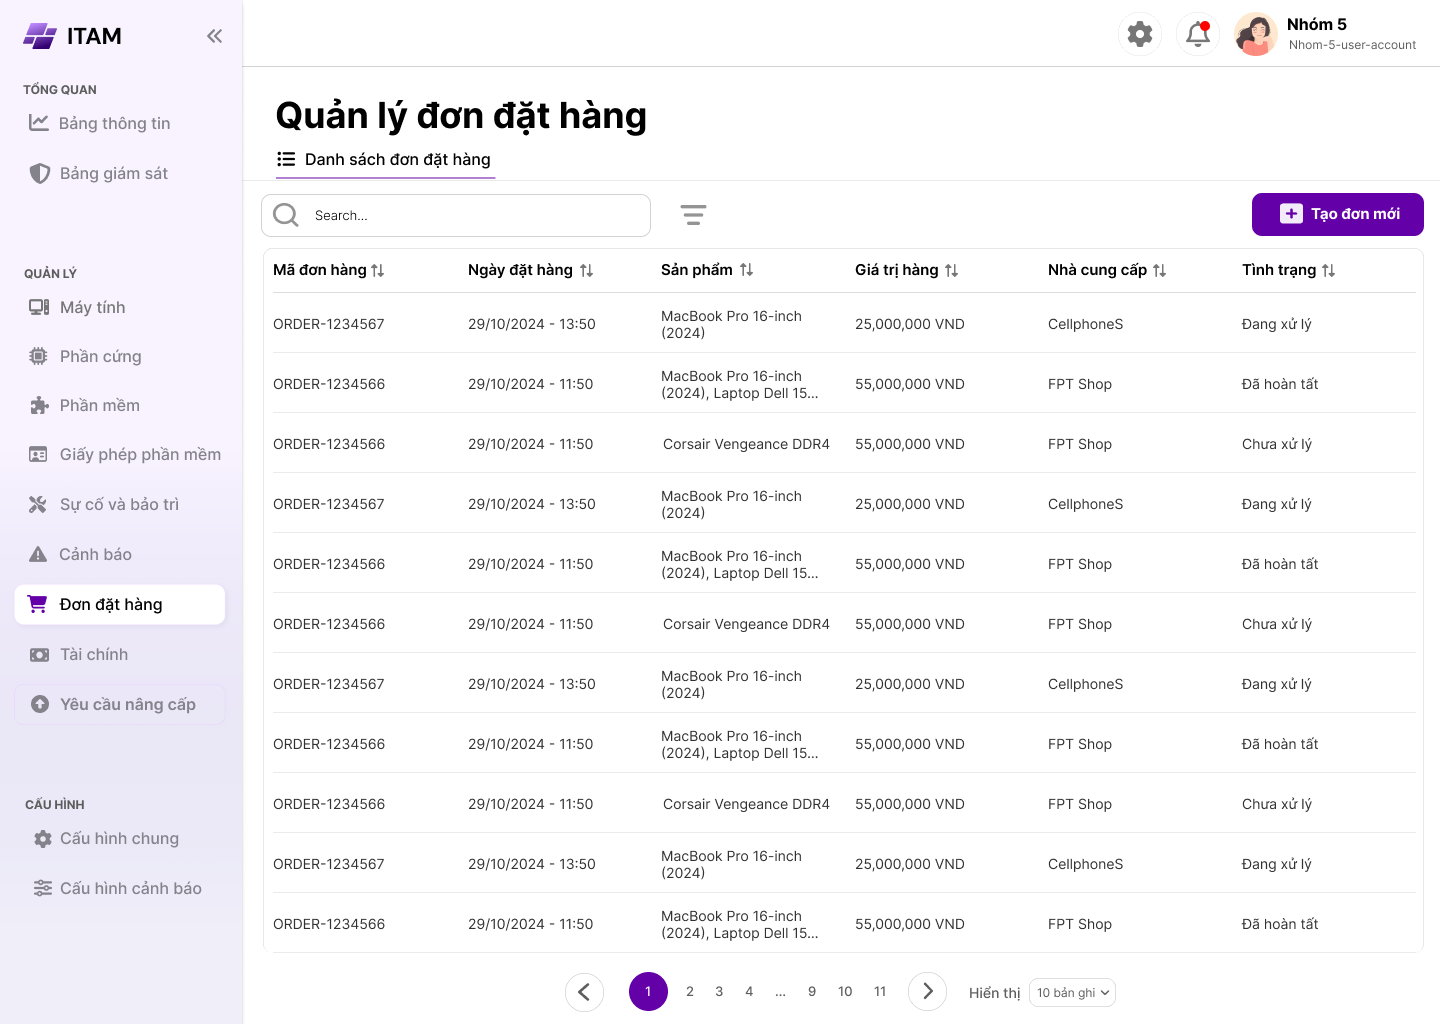
\includegraphics[width=14cm]{Images/C5/UI/Feature-Quản lý đơn đặt hàng 1.png}
%     \vspace{15pt}
%     \caption{Giao diện Quản lý đơn đặt hàng 1}
% \end{figure}
% \begin{figure}[H]
%     \centering
%     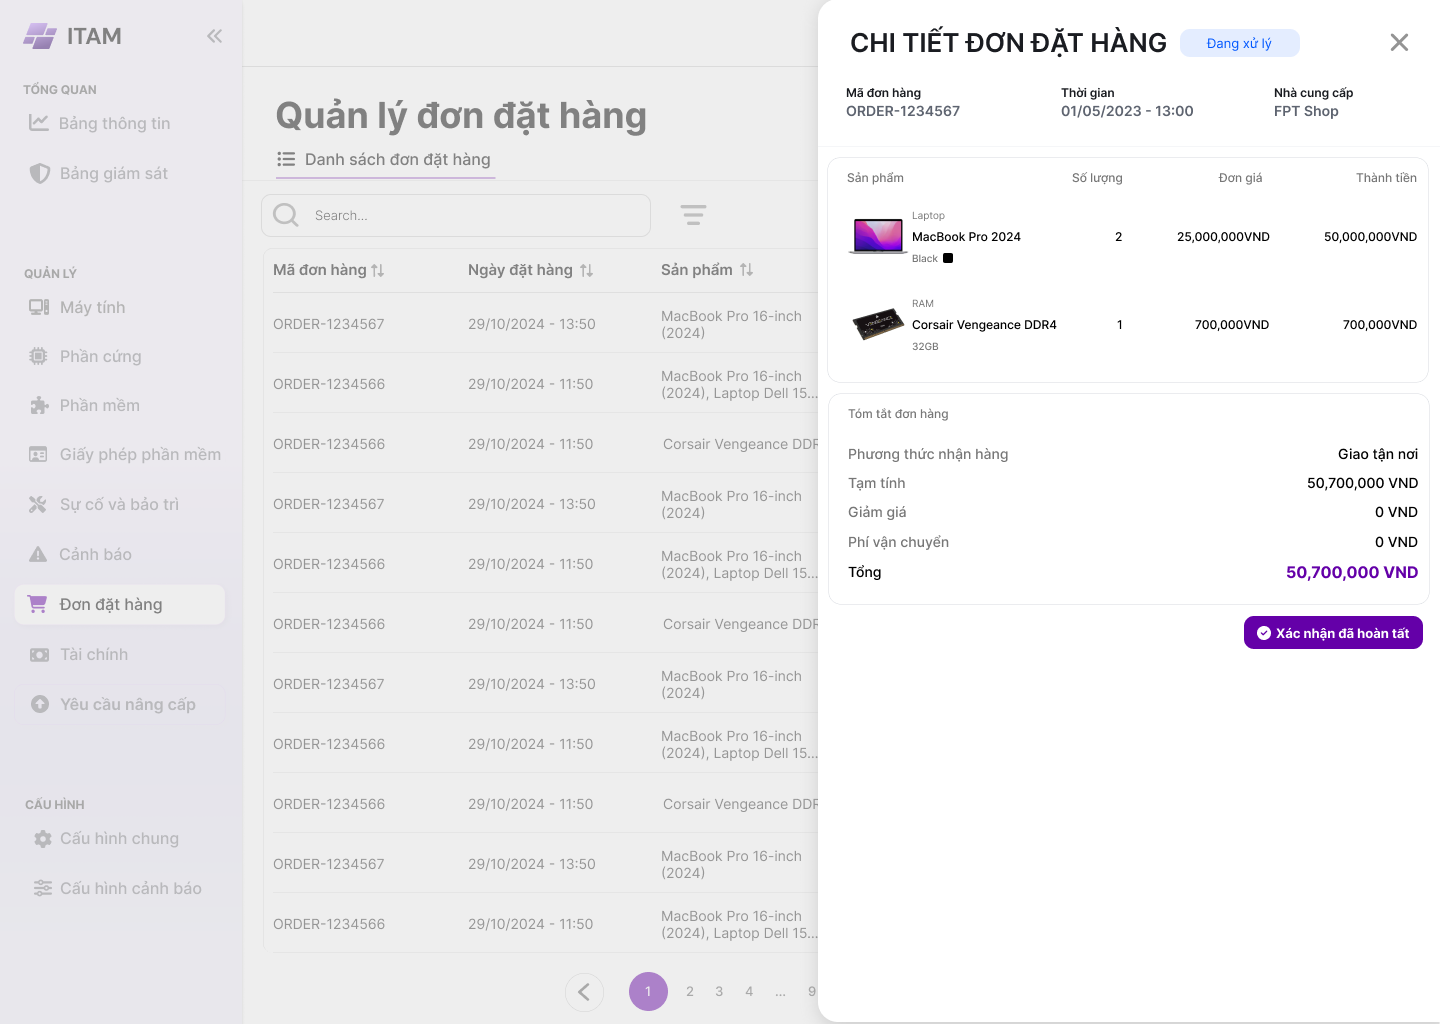
\includegraphics[width=14cm]{Images/C5/UI/Feature-Quản lý đơn đặt hàng 2.1.png}
%     \vspace{15pt}
%     \caption{Giao diện Quản lý đơn đặt hàng 2}
% \end{figure}
% \begin{figure}[H]
%     \centering
%     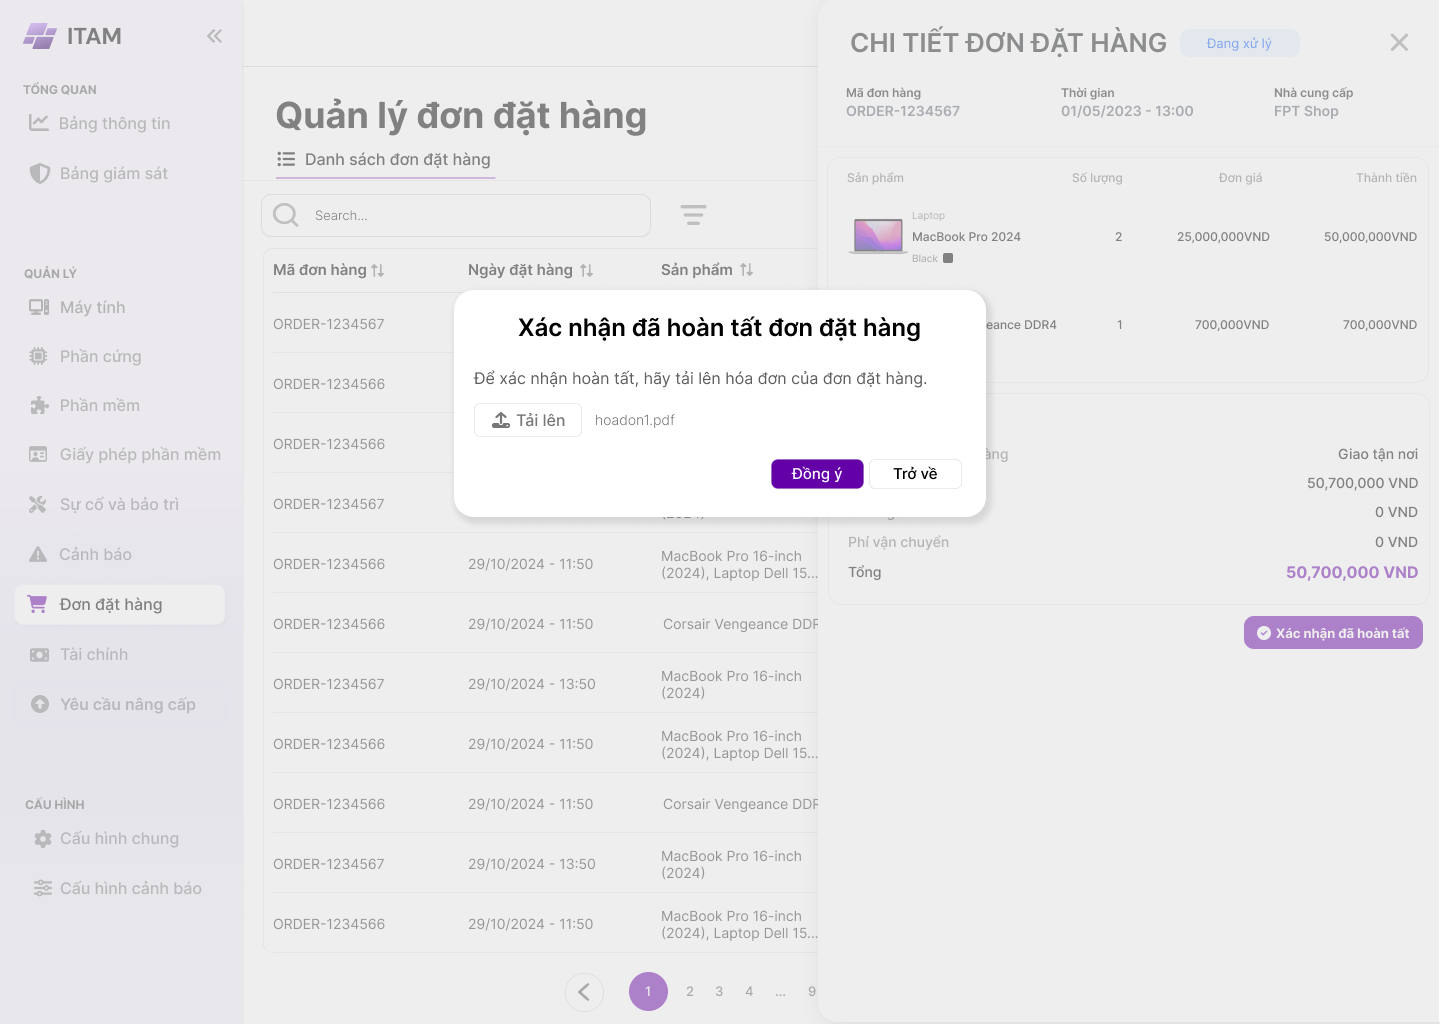
\includegraphics[width=14cm]{Images/C5/UI/Feature-Quản lý đơn đặt hàng 2.2.png}
%     \vspace{15pt}
%     \caption{Giao diện Quản lý đơn đặt hàng 3}
% \end{figure}
% \begin{figure}[H]
%     \centering
%     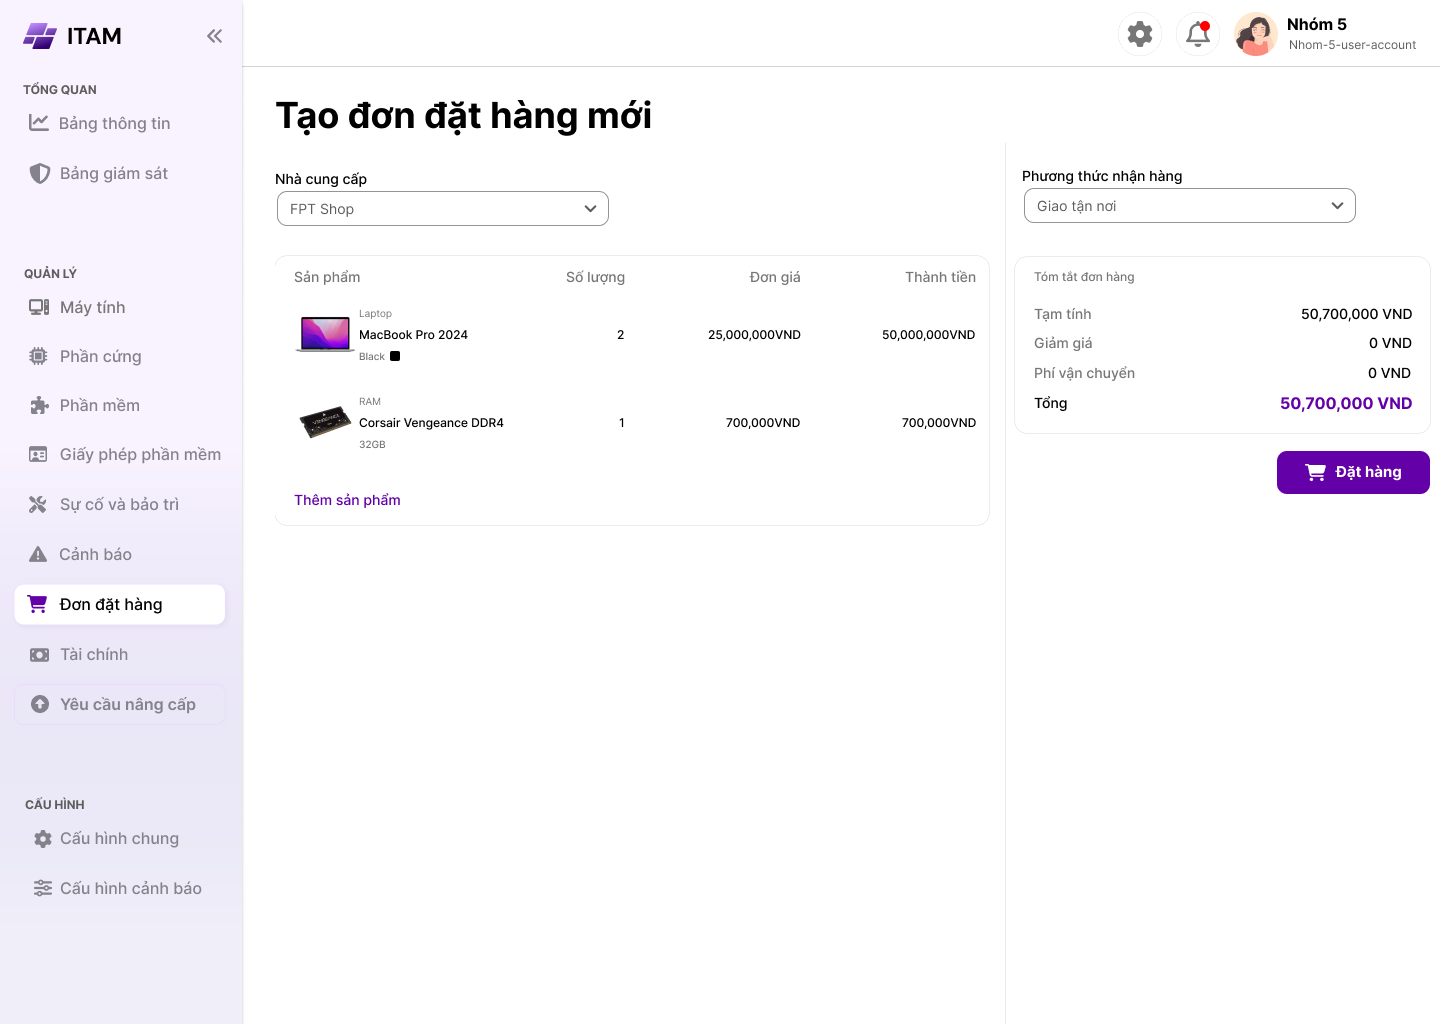
\includegraphics[width=14cm]{Images/C5/UI/Feature-Quản lý đơn đặt hàng 3.1.png}
%     \vspace{15pt}
%     \caption{Giao diện Quản lý đơn đặt hàng 3}
% \end{figure}
% \begin{figure}[H]
%     \centering
%     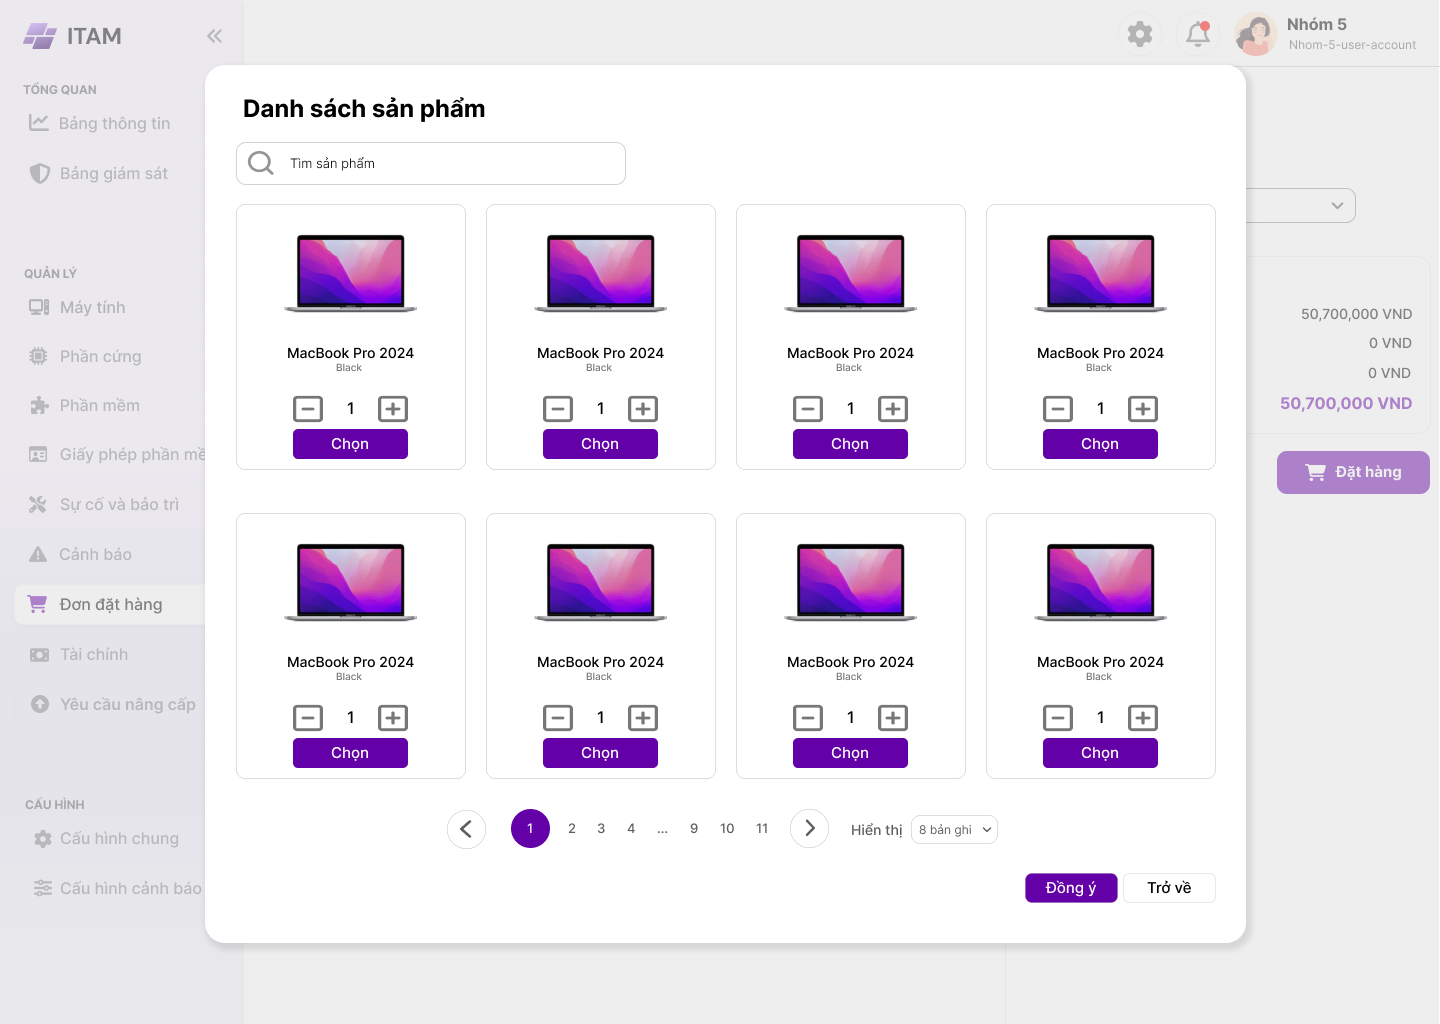
\includegraphics[width=14cm]{Images/C5/UI/Feature-Quản lý đơn đặt hàng 3.2.png}
%     \vspace{15pt}
%     \caption{Giao diện Quản lý đơn đặt hàng 5}
% \end{figure}
% \begin{figure}[H]
%     \centering
%     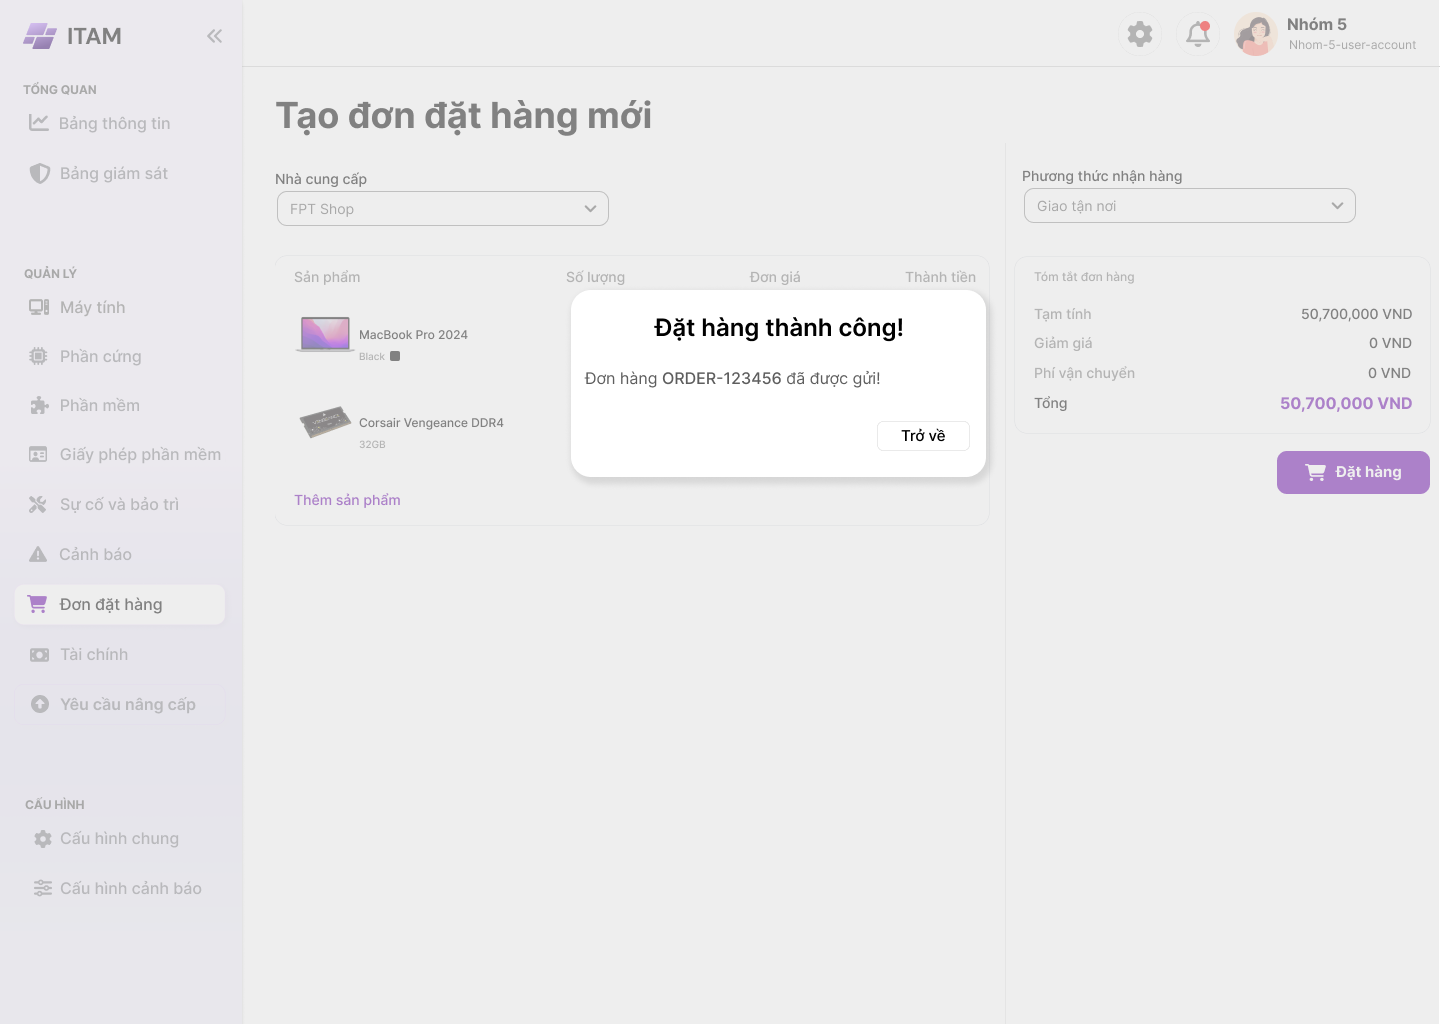
\includegraphics[width=14cm]{Images/C5/UI/Feature-Quản lý đơn đặt hàng 3.3.png}
%     \vspace{15pt}
%     \caption{Giao diện Quản lý đơn đặt hàng 6}
% \end{figure}

\item{Quản lý giấy phép phần mềm}\\
Quản lý giấy phép mềm hiển thị danh sách và thông tin của các giấy phép phần mềm có trong hệ thống (xem thêm chi tiết ở phụ lục).
% \begin{figure}[H]
%     \centering
%     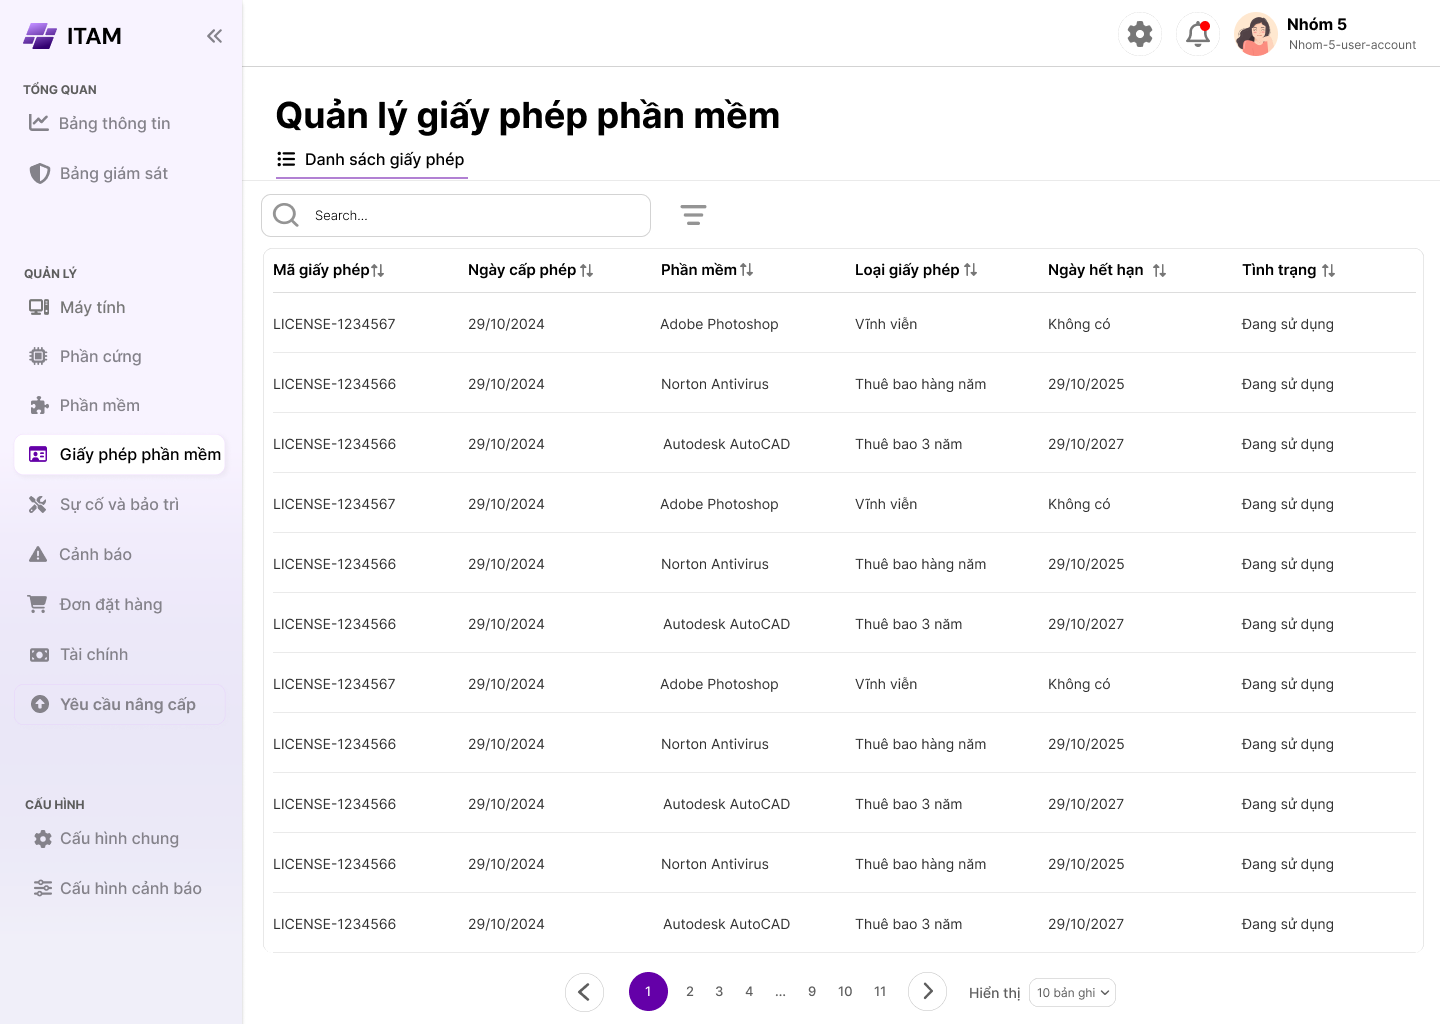
\includegraphics[width=14cm]{Images/C5/UI/Feature-Quản lý giấy phép phần mềm.png}
%     \vspace{15pt}
%     \caption{Giao diện Quản lý giấy phép phần mềm}
% \end{figure}

\item{Quản lý cấu hình cảnh báo}\\
Người dùng truy cập vào Cấu hình cảnh báo để điều chỉnh các ngưỡng của cảnh báo cho các máy tính trong hệ thống. Dựa vào các ngưỡng này, cảnh báo sẽ được sinh ra (xem thêm chi tiết ở phụ lục).
% \begin{figure}[H]
%     \centering
%     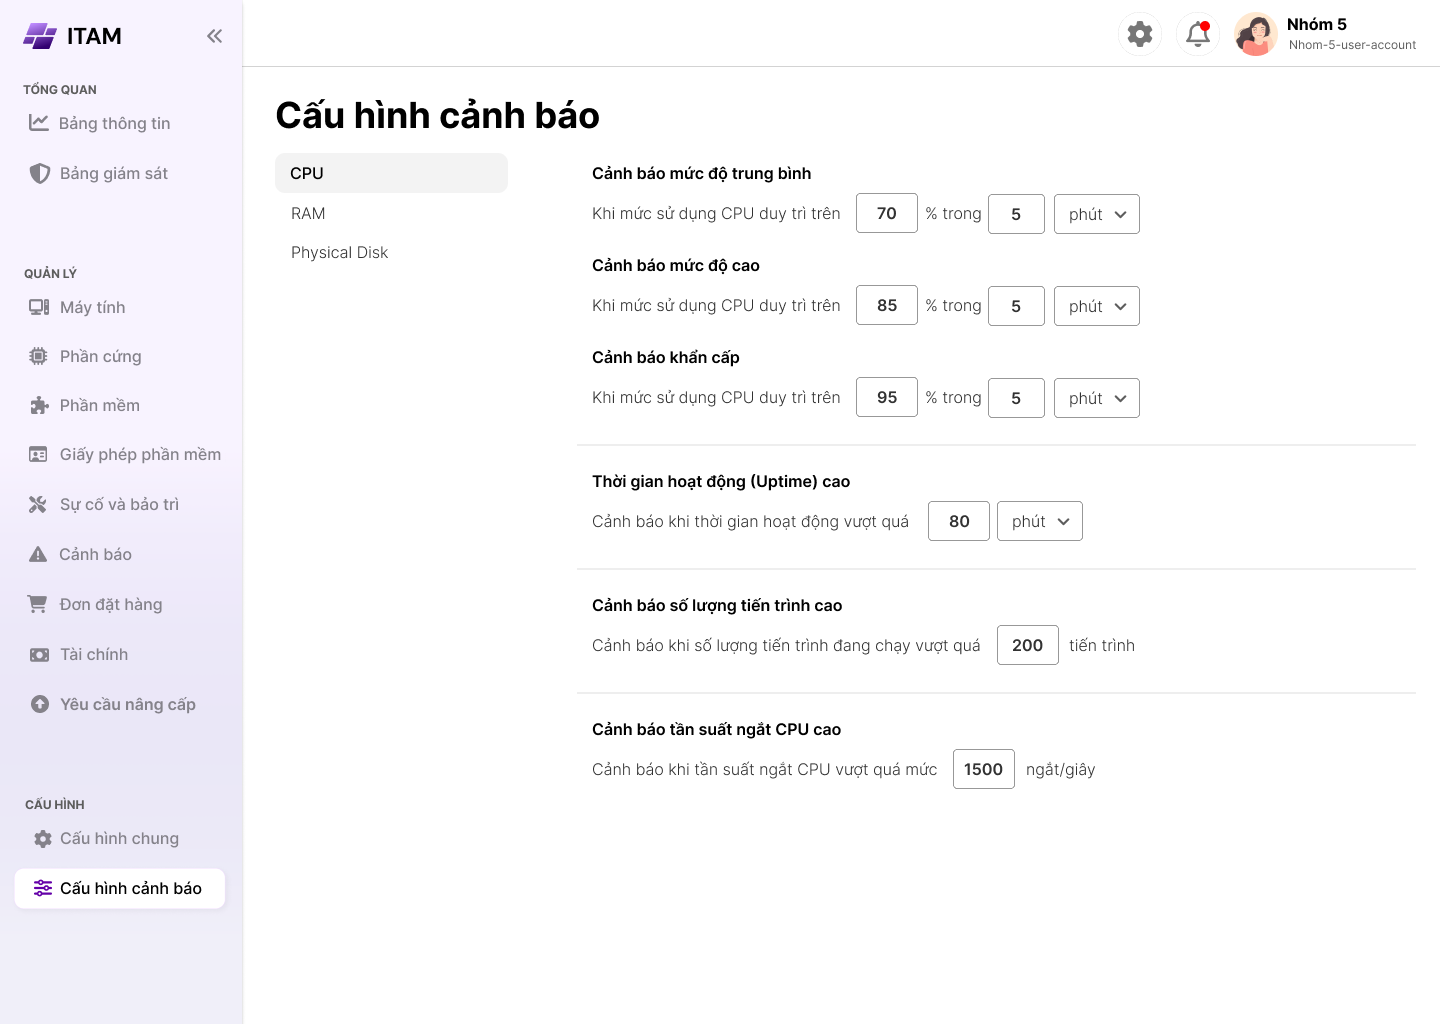
\includegraphics[width=14cm]{Images/C5/UI/Feature-Cấu hình cảnh báo 1.png}
%     \vspace{15pt}
%     \caption{Giao diện Quản lý cấu hình cảnh báo 1}
% \end{figure}
% \begin{figure}[H]
%     \centering
%     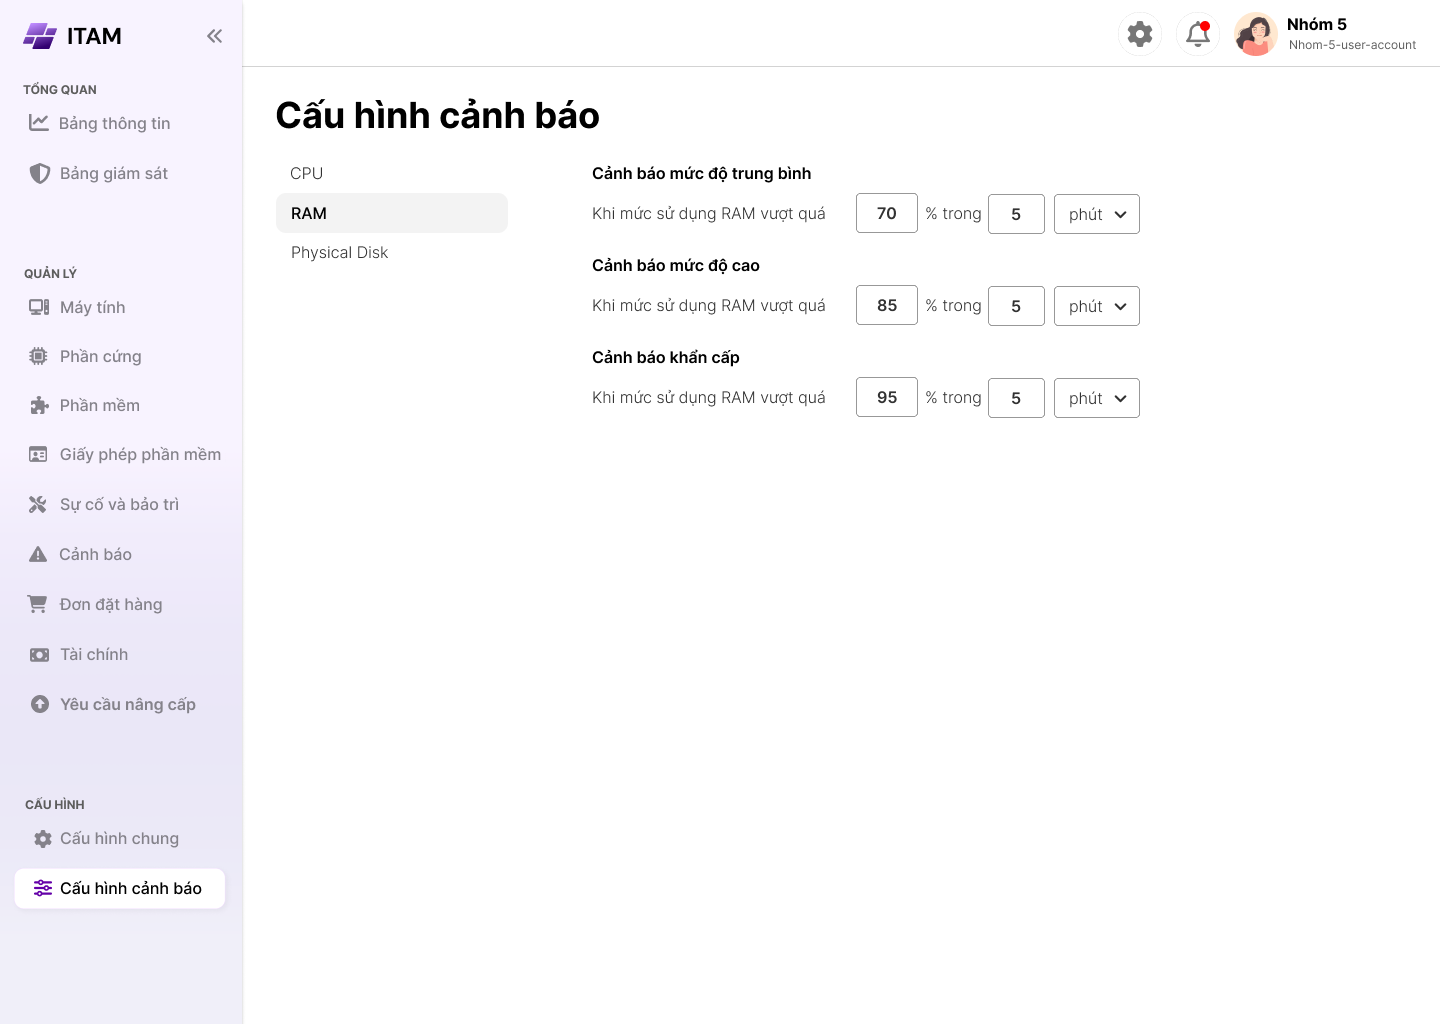
\includegraphics[width=14cm]{Images/C5/UI/Feature-Cấu hình cảnh báo 5.png}
%     \vspace{15pt}
%     \caption{Giao diện Quản lý cấu hình cảnh báo 2}
% \end{figure}
% \begin{figure}[H]
%     \centering
%     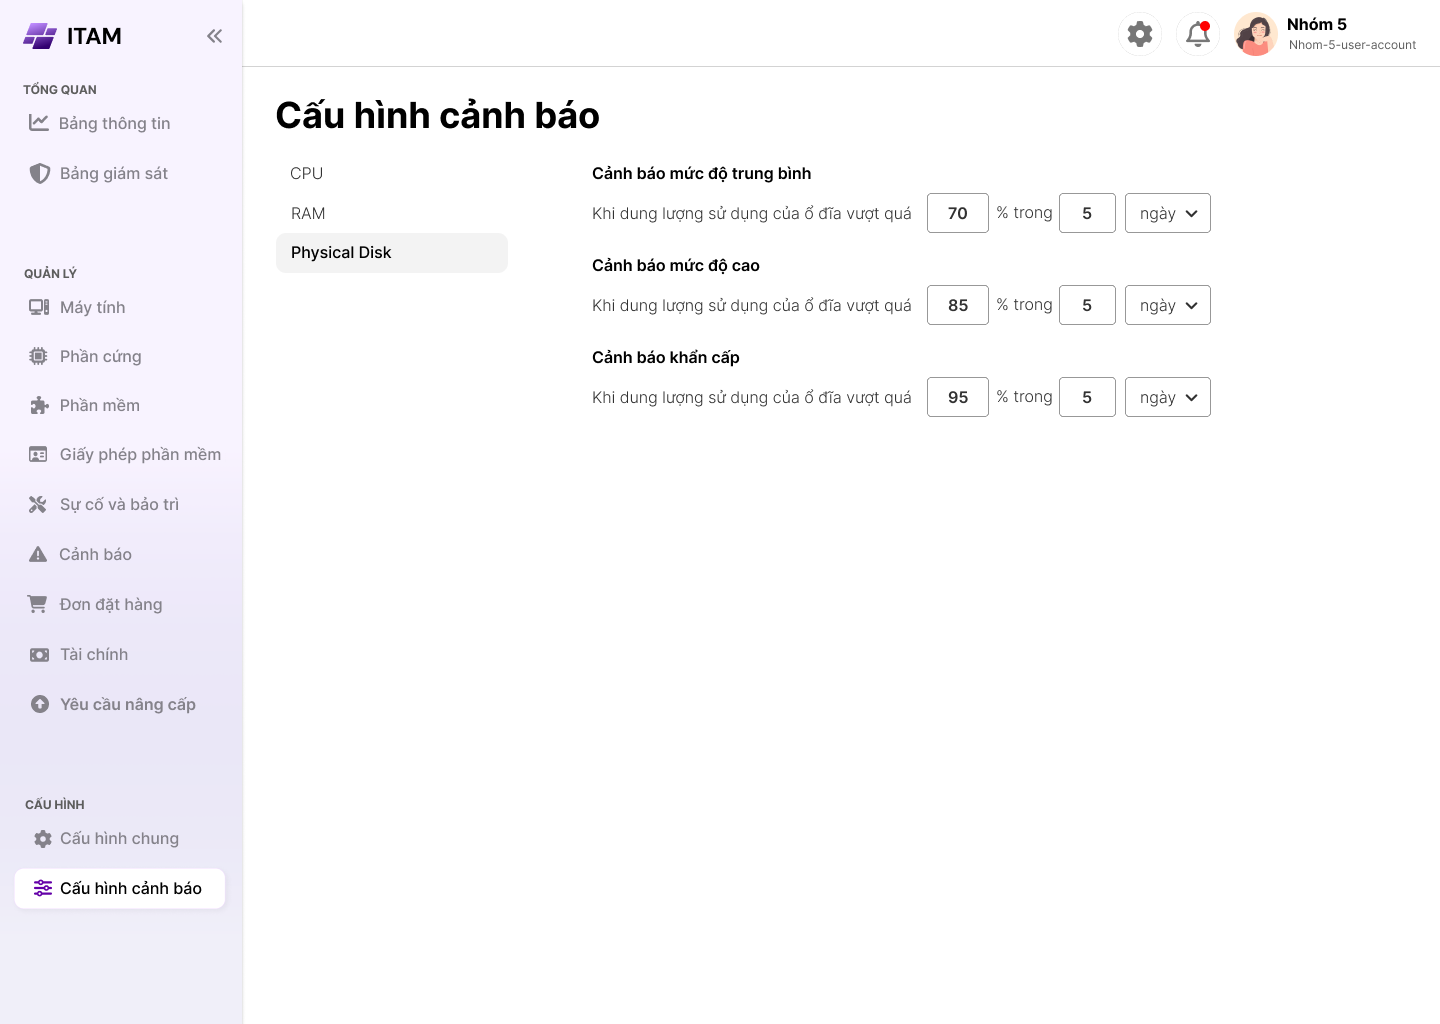
\includegraphics[width=14cm]{Images/C5/UI/Feature-Cấu hình cảnh báo 6.png}
%     \vspace{15pt}
%     \caption{Giao diện Quản lý cấu hình cảnh báo 3}
% \end{figure}

\end{itemize}
\subsection{Kết chương}
\noindent Trong quá trình phát triển một hệ thống hoàn chỉnh, phân tích và thiết kế đóng vai trò cốt lõi.
Chương này nhóm đã ba nội dung chính:
\begin{itemize}
    \item \textbf{Phân tích}: Mô hình hóa quy trình nghiệp vụ và các tương tác trong hệ thống.
    \item \textbf{Giải pháp công nghệ}: Đề xuất các giải pháp, đặc biệt là xử lý thời gian thực để đáp ứng yêu cầu nghiệp vụ.
    \item \textbf{Thiết kế}: Bao gồm thiết kế kiến trúc hệ thống, cơ sở dữ liệu, chi tiết bên trong và giao diện người dùng.
\end{itemize}
Qua phần phân tích nhóm đã đưa ra mô hình hóa nghiệp vụ cho các qui trình: giám sát tài sản, quản lý vòng đời tài sản, cảnh báo, quản lý đơn đặt hàng. Bên cạnh đó nhóm cũng đưa ra các use case cho hệ thống để trình bày các luồng thực thi cho hệ thống.\\ \\ 
Đến phần giải pháp công nghệ, nhóm đã trình bày các khái niệm, khía cạnh liên quan đến thu thập và xử lý dữ liệu thời gian thực. Ngoài ra nhóm cũng đã đi sâu vào phần công nghệ Kafka (công nghệ cốt lõi mà nhóm đã chọn) và so sánh Kafka với hai loại công nghệ khác là .\\ \\
Cuối cùng là phần thiết kế, trong phần này, nhóm đã đưa ra một kiến trúc hệ thống gồm 3 lớp là Presentation, Application, Storage. Từ đó nhóm đã lựa chọn các công nghệ cho Front-End là Angular và Back-end là ASP.NET Core, cơ sở dữ liệu là MSSQL. Nhóm cũng đã thiết kế ERD, làm rõ mối quan hệ giữa các đối tượng dữ liệu của hệ thống. Bên cạnh đó, nhóm cũng đã trình bày chi tiết bên trong qua class diagram và giao diện bên ngoài qua figma.







%  \newpage
% \section{Kết luận}

\subsection{Kết quả đạt được}

Nghiên cứu đã đề xuất, thiết kế và thực nghiệm thành công một kiến trúc giám sát lai nhằm giải quyết bài toán thẩm định cảnh báo bất thường trong môi trường cloud/server. Kiến trúc này kết hợp detector metric-only tốc độ cao ở tầng đầu, cơ chế Retrieval-Augmented Generation để truy xuất ngữ cảnh log/trace, và Mô hình Ngôn ngữ Lớn đóng vai trò Thẩm phán ngữ nghĩa. Bên cạnh đó, các cơ chế vận hành quan trọng như Context Rescue, Local-first với API fallback cũng đã được tích hợp và kiểm chứng.

Về mặt dữ liệu, nghiên cứu sử dụng Microsoft Cloud Monitoring Dataset như một benchmark để đánh giá năng lực phát hiện ban đầu của detector, trong khi Nezha Dataset được sử dụng làm tập dữ liệu chính cho các thí nghiệm hybrid nhờ tính đa chiều (metric, log, trace) và fault injection rõ ràng. Sự phân chia này giúp tách bạch giữa việc đánh giá baseline và đánh giá hiệu quả của pipeline RAG + LLM.

Về mặt thực nghiệm, kết quả khẳng định giả thuyết cốt lõi của đề tài: LLM không thể hoạt động hiệu quả như một tầng phán đoán độc lập khi thiếu ngữ cảnh. Các thí nghiệm \textit{LLM without RAG} cho thấy sự suy giảm nghiêm trọng về khả năng nhận diện \textit{true alert}. Ngược lại, cấu hình \textit{hybrid RAG} cải thiện rõ rệt F1-score và giảm False Positive Rate so với detector-only, chứng minh rằng việc thu hẹp "khoảng trống ngữ nghĩa" bằng ngữ cảnh vận hành là yếu tố tiên quyết để nâng cao chất lượng thẩm định cảnh báo.

\subsection{Ý nghĩa của Context Rescue và chiến lược vận hành}

Một trong những đóng góp nổi bật nhất của giai đoạn nghiên cứu này là cơ chế \textbf{Context Rescue}. Cơ chế này được đề xuất để khắc phục "điểm mù" của detector metric-only đối với các lỗi phi tài nguyên (như \textit{network\_delay}), nơi tín hiệu log/trace biểu hiện rõ ràng hơn metric tổng hợp. Thay vì chỉ thụ động xử lý các ứng viên do detector tạo ra, Context Rescue chủ động rà soát và chọn ra các cửa sổ metric bình thường thành ứng viên cảnh báo khi phát hiện tín hiệu ngữ cảnh đủ mạnh.

Kết quả trên Nezha Dataset cho thấy Context Rescue cải thiện vượt bậc Recall và F1-score, đồng thời loại bỏ hoàn toàn False Negative. Tuy nhiên, lợi ích này đi kèm với sự đánh đổi về chi phí vận hành do số lượng úng viên, lượt truy xuất ngữ cảnh và số lần gọi LLM gia tăng. Điều này khẳng định Context Rescue không phải là sự thay thế cho detector, mà là một cơ chế bổ trợ chiến lược nhằm giảm thiểu rủi ro bỏ sót sự cố trong các tình huống tín hiệu metric yếu nhưng tín hiệu ngữ cảnh mạnh.

Bên cạnh đó, chiến lược \textbf{Local-first} kết hợp API fallback đã chứng minh được tiềm năng trong việc tối ưu hóa chi phí và giảm sự phụ thuộc vào các mô hình thương mại. Tuy nhiên, thực nghiệm cũng chỉ ra rằng các mô hình cục bộ kích thước nhỏ (như qwen2.5:1.5b) chưa đủ độ ổn định để thay thế hoàn toàn API. Do đó, ở giai đoạn hiện tại, Local-first nên được định vị là một hướng kiểm chứng tính khả thi về mặt vận hành, làm tiền đề cho các cơ chế điều phối tài nguyên phức tạp hơn trong tương lai.

\subsection{Hạn chế của nghiên cứu}

Mặc dù các kết quả thực nghiệm đã chứng minh tính khả thi của kiến trúc đề xuất, nghiên cứu vẫn tồn tại một số hạn chế cần được khắc phục trong các giai đoạn tiếp theo:

\begin{itemize}
    \item \textbf{Giới hạn về môi trường thực nghiệm:} Hệ thống mới được đánh giá trong môi trường giả lập có kiểm soát thông qua cơ chế phát lại luồng. Mặc dù cơ chế watermark đã giúp ngăn chặn rò rỉ thông tin tương lai, nó chưa phản ánh đầy đủ các thách thức của môi trường streaming thực tế như backpressure, sự kiện đến không theo thứ tự hay độ trễ hàng đợi.
    \item \textbf{Quy mô và tính chất của các kịch bản:} Một số thí nghiệm (như Local-first và streaming replay) chủ yếu đóng vai trò kiểm chứng luồng vận hành chứ chưa phải là các benchmark quy mô lớn. Đặc biệt, Context Rescue là một cải tiến mang tính hệ thống, làm thay đổi cả quy trình tạo candidate và chi phí gọi LLM, do đó khó để đánh giá dưới dạng một thí nghiệm cắt bỏ đơn biến thuần túy.
    \item \textbf{Thiếu hụt các chỉ số đánh giá chiều sâu của RAG:} Chất lượng truy xuất ngữ cảnh hiện mới chỉ được đánh giá ở mức vĩ mô (context coverage, retrieval latency). Các chỉ số vi mô về mức độ khớp của bằng chứng  như \textit{evidence hit@k}, \textit{service match}, hay \textit{time-window match} chưa được đo lường đầy đủ.
    \item \textbf{Rào cản từ đặc tính của LLM:} Việc ứng dụng LLM vẫn chịu ảnh hưởng bởi chi phí token, giới hạn quota, rate limit và tính không tất định trong đầu ra. Các cơ chế LLMOps như semantic cache, scheduler ưu tiên và manual review cần được hoàn thiện hơn nữa để đáp ứng yêu cầu của môi trường production.
\end{itemize}

\subsection{Kết luận chung}

Tổng kết lại, nghiên cứu đã chứng minh tính khả thi ban đầu của một pipeline AIOps lai cho bài toán thẩm định cảnh báo bất thường trên dữ liệu giám sát cloud/server. Kết quả thực nghiệm cho thấy detector metric-only đóng vai trò tối ưu trong việc tạo ứng viên nhanh chóng, nhưng không đủ năng lực để đưa ra quyết định cảnh báo cuối cùng do thiếu hụt ngữ cảnh vận hành. Việc tích hợp RAG và LLM-as-a-Judge giúp hệ thống khai thác hiệu quả log/trace context, trong khi Context Rescue mở rộng biên độ phát hiện bằng cách khôi phục các ứng viên bị bỏ sót.

Quan trọng hơn, nghiên cứu chỉ ra rằng bài toán giám sát lai trong thời gian thực không chỉ đơn thuần là tối ưu hóa các chỉ số Precision, Recall hay F1-score, mà thực chất là một \textbf{bài toán đánh đổi đa mục tiêu} giữa chất lượng cảnh báo, chi phí suy luận, độ trễ và độ tin cậy của hệ thống. Do đó, kiến trúc tối ưu không phải là đưa toàn bộ dữ liệu thô vào LLM, mà là thiết kế một kiến trúc phễu lọc, nơi LLM được sử dụng một cách có chọn lọc và thông minh sau các tầng sàng lọc, truy xuất và kiểm soát chi phí.

Trong các giai đoạn tiếp theo, đề tài sẽ tập trung vào việc hình thức hóa cơ chế Context Rescue, bổ sung các chỉ số đánh giá bằng chứng chuyên sâu, phát triển RCA Post-processing Agent và chuyển dịch sang môi trường True Streaming với fault injection chủ động. Những hướng mở rộng này sẽ giúp hệ thống tiến từ bài toán thẩm định cảnh báo đơn lẻ sang bài toán hỗ trợ chẩn đoán và hiểu sự cố, hướng tới một khung giải pháp AIOps hoàn chỉnh và có tính ứng dụng thực tiễn cao.
% \section{Hiện thực và kiểm thử}
% \subsection{Thiết kế API}
% \noindent Dưới đây là trình bày chi tiết thiết kế các giao diện lập trình ứng dụng (API) được sử dụng trong hệ thống. Thiết kế đầy đủ của toàn bộ hệ thống được trình bày tại đây \href{https://app.swaggerhub.com/apis/ITAMhcmut/APIDesign/1.0.0}{Link}.
% \subsubsection{Quản lý người dùng}
%     \begin{enumerate}
%         \item \textbf{Đăng nhập}
%         \begin{itemize}[label=--]
%             \item \textbf{URL:} \texttt{/api/login}
%             \item \textbf{Method:} POST
%             \item \textbf{Description:} API dùng để xác thực thông tin đăng nhập của người dùng.            
%             \item \textbf{Authorization:}
%             \begin{itemize}[label=\textbullet]
%                 \item Yêu cầu: Không yêu cầu
%                 \item Quyền truy cập: Mọi người dùng đều có thể gọi API này để đăng nhập.
%             \end{itemize}
%             \item \textbf{Request:} 
%             \begin{itemize}[label=\textbullet]
%                 \item Content-Type: \texttt{application/json}
%                 \item Request Body:
%             \end{itemize}
%             \begin{longtable}{|l|l|l|l|}
%             \hline
%             \textbf{Trường} & \textbf{Kiểu} & \textbf{Mô tả} & \textbf{Bắt buộc} \\
%             \hline
%             \endhead
%             \texttt{email} & String & Địa chỉ email người dùng & Có \\
%             \texttt{password} & String & Mật khẩu đăng nhập & Có \\
%             \hline
%             \end{longtable}
%             \item \textbf{Responses:}
%             \begin{itemize}[label=\textbullet]
%                 \item \textbf{200 OK:} Đăng nhập thành công. Dữ liệu JSON trả về:
%                 \begin{longtable}{|l|l|l|}
%                 \hline
%                 \textbf{Trường} & \textbf{Kiểu} & \textbf{Mô tả} \\
%                 \hline
%                 \endhead
%                 \texttt{accessToken} & String & Token JWT dùng để xác thực truy cập \\
%                 \hline
%                 \texttt{refreshToken} & String & Token để làm mới \texttt{accessToken}\\
%                 \hline
%                 \end{longtable}
%                 \item \textbf{500 Internal Server Error:} Có lỗi xảy ra trong quá trình xử lý hoặc người dùng không được phép đăng nhập. Không có dữ liệu trả về.
%             \end{itemize}
%         \end{itemize}
%         \item \textbf{Truy vấn thông tin của người dùng}
%         \begin{itemize}[label=--]
%             \item \textbf{URL:} \texttt{/api/users/\{id\}}
%             \item \textbf{Method:} GET
%             \item \textbf{Description:} Lấy thông tin chi tiết của người dùng cụ thể dựa trên \texttt{id}.            
%             \item \textbf{Authorization:}
%             \begin{itemize}[label=\textbullet]
%                 \item Yêu cầu: Header Authorization: Bearer <\texttt{accessToken}>
%                 \item Quyền truy cập: Administrator, Manager
%                 \item Phản hồi nếu không đủ quyền: 403 Forbidden
%             \end{itemize}
%             \item \textbf{Parameters:}
%             \begin{longtable}{|l|l|l|l|l|}
%             \hline
%             \textbf{Tên tham số} & \textbf{Vị trí} & \textbf{Kiểu dữ liệu} & \textbf{Bắt buộc} & \textbf{Mô tả} \\
%             \hline
%             \endhead
%             \texttt{id} & Path & String & Có & ID của người dùng\\
%             \hline
%             \end{longtable}
%             \item \textbf{Responses:}
%             \begin{itemize}[label=\textbullet]
%                 \item \textbf{200 OK:} Lấy thông tin thành công. Trả về dữ liệu chi tiết của người dùng.
%                 \begin{longtable}{|l|l|l|}
%                 \hline
%                 \textbf{Trường} & \textbf{Kiểu} & \textbf{Mô tả} \\
%                 \hline
%                 \endhead
%                 \texttt{id} & String & ID của người dùng \\
%                 \texttt{firstName} & String & Họ của người dùng \\
%                 \texttt{lastName} & String & Tên của người dùng \\
%                 \texttt{role} & String & Vai trò của người dùng \\
%                 \texttt{phoneNumber} & String & Số điện thoại người dùng \\
%                 \texttt{createdAt} & String & Ngày tạo tài khoản (ISO format) \\
%                 \texttt{lastUpdatedAt} & String & Ngày cập nhật gần nhất \\
%                 \texttt{accessToken} & String & Token xác thực truy cập \\
%                 \texttt{refreshToken} & String & Token làm mới \\                
%                 \hline
%                 \end{longtable}
%                 \item \textbf{403 Forbidden:} Người dùng không có quyền truy cập tài nguyên này. Không có dữ liệu trả về.
%                 \item \textbf{500 Internal Server Error} - Có lỗi xảy ra trong quá trình truy vấn người dùng. Không có dữ liệu trả về 
%             \end{itemize}
%         \end{itemize}
%     \end{enumerate}
% \subsubsection{Quản lý tài sản}
%     \begin{enumerate}
%         \item \textbf{Tạo mới máy tính}
%         \begin{itemize}[label=--]
%             \item \textbf{URL:} \texttt{/api/computer/CreateComputer}
%             \item \textbf{Method:} POST
%             \item \textbf{Description:} Tạo mới một tài sản máy tính
%             \item \textbf{Authorization:}
%             \begin{itemize}[label=\textbullet]
%                 \item Yêu cầu: Authorization: Bearer <\texttt{accessToken}>
%                 \item Quyền truy cập: Administrator, ITStaff
%                 \item Phản hồi nếu không đủ quyền: 403 Forbidden
%             \end{itemize}
%             \item \textbf{Request:}
%             \begin{itemize}[label=\textbullet]
%                 \item Content-Type: \texttt{application/json}
%                 \item Request Body:
%             \end{itemize}
%             \begin{longtable}{|l|l|l|l|}
%             \hline
%             \textbf{Trường} & \textbf{Kiểu} & \textbf{Mô tả} & \textbf{Bắt buộc} \\
%             \hline
%             \endhead
%             \texttt{name} & String & Tên thiết bị (do người dùng đặt) & Có \\
%             \texttt{model} & String & Model của máy tính & Không \\
%             \texttt{serialNumber} & String & Số serial & Không \\
%             \texttt{os} & String & Hệ điều hành & Không \\
%             \texttt{computerType} & String & Loại máy tính (Laptop, Desktop) & Có \\
%             \hline
%             \end{longtable}
%             \item \textbf{Responses:}
%             \begin{itemize}[label=\textbullet]
%                 \item \textbf{200 OK:} Tạo thành công. Trả về thông tin chi tiết của máy tính vừa được tạo. 
%                 \begin{longtable}{|l|l|l|}
%                 \hline
%                 \textbf{Trường} & \textbf{Kiểu} & \textbf{Mô tả} \\
%                 \hline
%                 \endhead
%                 \texttt{assetId} & String & Mã định danh của thiết bị \\
%                 \texttt{name} & String & Tên thiết bị \\
%                 \texttt{mac} & String & Địa chỉ MAC \\
%                 \texttt{ip} & String & Địa chỉ IP \\
%                 \texttt{bios} & String & Thông tin BIOS \\
%                 \texttt{model} & String & Model thiết bị \\
%                 \texttt{serialNumber} & String & Số serial \\
%                 \texttt{os} & String & Hệ điều hành \\
%                 \texttt{computerType} & String & Loại máy tính \\
%                 \texttt{currentUser} & String & Người dùng hiện tại \\
%                 \texttt{status} & String & Trạng thái thiết bị \\
%                 \texttt{hardware} & Array[Object] & Thông tin phần cứng chi tiết \\
%                 \hline
%                 \end{longtable}
%                 \item \textbf{403 Forbidden:} Người dùng không có quyền tạo máy tính. Không có dữ liệu trả về.
%                 \item \textbf{500 Internal Server Error:} Dữ liệu đầu vào không hợp lệ hoặc có lỗi trong quá trình xử lý. Không có dữ liệu trả về.
%             \end{itemize}
%         \end{itemize}
%         \item \textbf{Truy vấn thông tin phần cứng}
%         \begin{itemize}[label=--]
%             \item \textbf{URL:} \texttt{/api/hardware/GetHardwares}
%             \item \textbf{Method:} GET
%             \item \textbf{Description:} API này dùng để truy vấn danh sách phần cứng từ hệ thống, hỗ trợ phân trang, tìm kiếm và sắp xếp.
%             \item \textbf{Authorization:}
%             \begin{itemize}[label=\textbullet]
%                 \item Yêu cầu: Header Authorization: Bearer <\texttt{accessToken}>.
%                 \item Quyền truy cập: Administrator, Manager, ITStaff.
%                 \item Phản hồi nếu không đủ quyền: 403 Forbidden.
%             \end{itemize}
%             \item \textbf{Parameters:}
%             \begin{longtable}{|l|l|l|l|l|}
%             \hline
%             \textbf{Tên tham số} & \textbf{Vị trí} & \textbf{Kiểu} & \textbf{Bắt buộc} & \textbf{Mô tả} \\
%             \hline
%             \endhead
%             \texttt{page} & Query & Number & Không & Số trang hiện tại\\
%             \texttt{pageSize} & Query & Number & Không & Số phần tử mỗi trang \\
%             \texttt{search} & Query & String & Không & Từ khóa tìm kiếm\\
%             \texttt{sortColumn} & Query & String & Không & 	Cột dùng để sắp xếp \\
%             \texttt{sortOrder} & Query & String & Không & \texttt{asc} hoặc \texttt{desc}\\
%             \hline
%             \end{longtable}
%             \item \textbf{Responses:}
%             \begin{itemize}[label=\textbullet]
%                 \item \textbf{200 OK:} Lấy dữ liệu thành công. Trả về danh sách phần cứng và thông tin phân trang.
%                 \begin{longtable}{|l|l|l|}
%                 \hline
%                 \textbf{Trường} & \textbf{Kiểu} & \textbf{Mô tả} \\
%                 \hline
%                 \endhead
%                 \texttt{items} & Array[Object] & Danh sách phần cứng\\
%                 \texttt{totalRecords} & Number & Tổng số phần cứng trong hệ thống \\
%                 \texttt{currentPage} & Number & Trang hiện tại \\
%                 \texttt{pageSize} & Number & Số phần tử mỗi trang \\
%                 \texttt{totalPages} & Number & Tổng số trang \\
%                 \hline
%                 \end{longtable}
%                 Mỗi phần tử trong \texttt{items} sẽ là một object phần cứng, bao gồm:
%                 \begin{longtable}{|l|l|l|}
%                 \hline
%                 \textbf{Trường} & \textbf{Kiểu} & \textbf{Mô tả} \\
%                 \hline
%                 \endhead
%                 \texttt{serialNumber} & String & Số serial của phần cứng \\
%                 \texttt{computerID} & String & ID máy tính đang gắn phần cứng \\
%                 \texttt{hardwareType} & String & Loại phần cứng \\
%                 \texttt{usingStatus} & String & Trạng thái sử dụng \\
%                 \texttt{manufacturer} & String & Hãng sản xuất \\
%                 \texttt{details} & String & Thông tin chi tiết \\
%                 \texttt{assetId} & String & Mã định danh tài sản liên quan \\
%                 \texttt{name} & String & Tên định danh của phần cứng trong hệ thống \\
%                 \hline
%                 \end{longtable}
%                 \item \textbf{403 Forbidden:} Người dùng không có quyền truy cập API. Không có dữ liệu trả về.
%                 \item \textbf{500 Internal Server Error:} Dữ liệu đầu vào không hợp lệ hoặc có lỗi trong quá trình xử lý. Không có dữ liệu trả về.
%             \end{itemize}
%         \end{itemize}
%     \end{enumerate}
% \subsubsection{Yêu cầu nâng cấp tài sản}
%     \begin{enumerate}
%         \item \textbf{Tạo yêu cầu nâng cấp phần mềm}
%         \begin{itemize}[label=--]
%             \item \textbf{URL:} \texttt{/api/UpgradeRequest/software}
%             \item \textbf{Method:} POST
%             \item \textbf{Description:} API dùng để tạo mới một yêu cầu nâng cấp phần mềm cho thiết bị (tài sản).
%             \item \textbf{Authorization:}
%             \begin{itemize}[label=\textbullet]
%                 \item Yêu cầu: Header Authorization: Bearer <\texttt{accessToken}>.
%                 \item Quyền truy cập: Administrator, ITStaff.
%                 \item Phản hồi nếu không đủ quyền: 403 Forbidden.
%             \end{itemize}
%             \item \textbf{Request:}
%             \begin{itemize}[label=\textbullet]
%                 \item Content-Type: \texttt{application/json}
%                 \item Request Body:
%             \end{itemize}
%             \begin{longtable}{|l|l|l|l|}
%             \hline
%             \textbf{Trường} & \textbf{Kiểu} & \textbf{Mô tả} & \textbf{Bắt buộc} \\
%             \hline
%             \endhead
%             \texttt{description} & String & Mô tả ngắn gọn yêu cầu nâng cấp & Không \\
%             \texttt{updateReason} & String & Lý do cần nâng cấp phần mềm & Không \\
%             \texttt{assetId} & String & ID của thiết bị & Có \\
%             \texttt{updateType} & String & Loại cập nhật & Có \\
%             \texttt{managerName} & String & Tên người quản lý phê duyệt & Có \\
%             \texttt{staffName} & String & Tên nhân viên tạo yêu cầu & Có \\
%             \texttt{softwareType} & String & Loại phần mềm yêu cầu nâng cấp & Có\\
%             \texttt{softwareAlt} & String & ID của phần mềm nâng cấp & Có \\
%             \hline
%             \end{longtable}
%             \item \textbf{Responses:}
%             \begin{itemize}[label=\textbullet]
%                 \item \textbf{200 OK:} Tạo yêu cầu thành công. Trả về thông tin của yêu cầu nâng cấp vừa tạo.
%                 \begin{longtable}{|l|l|l|}
%                 \hline
%                 \textbf{Trường} & \textbf{Kiểu} & \textbf{Mô tả} \\
%                 \hline
%                 \endhead
%                 \texttt{requestId} & String & ID của yêu cầu nâng cấp \\
%                 \texttt{staffName} & String & Tên nhân viên gửi yêu cầu \\
%                 \texttt{managerName} & String & Tên người quản lý sẽ phê duyệt hoặc từ chối yêu cầu \\
%                 \texttt{createdDate} & String & Ngày tạo yêu cầu (ISO Format) \\
%                 \texttt{approvedDate} & String & Ngày yêu cầu được phê duyệt (nếu có) \\
%                 \texttt{rejectedDate} & String & Ngày yêu cầu bị từ chối (nếu có) \\
%                 \texttt{status} & String & Trạng thái hiện tại của yêu cầu \\
%                 \texttt{description} & String & Mô tả nội dung yêu cầu \\
%                 \texttt{updateReason} & String & Lý do đề xuất nâng cấp phần mềm \\
%                 \texttt{updateType} & String & Loại nâng cấp \\
%                 \texttt{typeDetail} & String & Thông tin chi tiết hơn về phần mềm cần nâng cấp \\
%                 \hline
%                 \end{longtable}
%                 \item \textbf{403 Forbidden:} Người dùng không có quyền truy cập API. Không có dữ liệu trả về.
%                 \item \textbf{500 Internal Server Error:} Dữ liệu đầu vào không hợp lệ hoặc có lỗi trong quá trình xử lý. Không có dữ liệu trả về.
%             \end{itemize}
%         \end{itemize}
%         \item \textbf{Hủy yêu cầu nâng cấp}
%         \begin{itemize}[label=--]
%             \item \textbf{URL:} \texttt{/api/UpgradeRequest/cancel/\{id\}}
%             \item \textbf{Method:} PUT
%             \item \textbf{Description:} Hủy một yêu cầu nâng cấp chưa được xử lý (trạng thái còn Pending).
%             \item \textbf{Authorization:}
%             \begin{itemize}[label=\textbullet]
%                 \item Yêu cầu: Header Authorization: Bearer <\texttt{accessToken}>.
%                 \item Quyền truy cập: Administrator, ITStaff.
%                 \item Phản hồi nếu không đủ quyền: 403 Forbidden.                
%             \end{itemize}
%             \item \textbf{Parameters:}
%             \begin{longtable}{|l|l|l|l|l|}
%             \hline
%             \textbf{Tên tham số} & \textbf{Vị trí} & \textbf{Kiểu} & \textbf{Bắt buộc} & \textbf{Mô tả} \\
%             \hline
%             \endhead
%             \texttt{id} & Path & String & Có & ID của yêu cầu cần hủy \\
%             \hline
%             \end{longtable}
%             \item \textbf{Responses:}
%             \begin{itemize}[label=\textbullet]
%                 \item \textbf{200 OK:} Hủy yêu cầu thành công. Trả về thông tin của yêu cầu đã cập nhật trạng thái.
%                 \item \textbf{403 Forbidden:} Người dùng không có quyền truy cập API. Không có dữ liệu trả về.
%                 \item \textbf{500 Internal Server Error:} Dữ liệu đầu vào không hợp lệ hoặc có lỗi trong quá trình xử lý. Không có dữ liệu trả về.
%             \end{itemize}
%         \end{itemize}
%     \end{enumerate}
% \subsubsection{Quản lý đơn đặt hàng}
%     \begin{enumerate}
%         \item \textbf{Tạo mới đơn đặt hàng}
%         \begin{itemize}[label=--]
%             \item \textbf{URL:} \texttt{/api/purchase-order/new}
%             \item \textbf{Method:} POST
%             \item \textbf{Description:} API dùng để tạo mới một đơn mua hàng với thông tin nhà cung cấp, các mặt hàng và chi phí liên quan.
%             \item \textbf{Authorization:}
%             \begin{itemize}[label=\textbullet]
%                 \item Yêu cầu: Header Authorization: Bearer <\texttt{accessToken}>.
%                 \item Quyền truy cập: Administrator, Manager
%                 \item Phản hồi nếu không đủ quyền: 403 Forbidden.
%             \end{itemize}
%             \item \textbf{Request:}
%             \begin{itemize}[label=\textbullet]
%                 \item Content-Type: \texttt{application/json}
%                 \item Request Body:
%             \end{itemize}
%             \begin{longtable}{|l|l|l|l|}
%             \hline
%             \textbf{Trường} & \textbf{Kiểu} & \textbf{Mô tả} & \textbf{Bắt buộc} \\
%             \hline
%             \endhead
%             \texttt{orderDate} & String &  Ngày tạo đơn (ISO Format) & Có  \\
%             \texttt{shippingCost} & Number & Chi phí vận chuyển & Có \\
%             \texttt{totalCost} & Number & Tổng chi phí đơn hàng & Có \\
%             \texttt{status} & String & Trạng thái đơn hàng & Có \\
%             \texttt{supplier} & Object & Thông tin nhà cung cấp & Có \\
%             \texttt{orderItems} & Array[Object] & Danh sách các mặt hàng đặt mua & Có \\
%             \hline
%             \end{longtable}
%             \item \textbf{Responses:} 
%             \begin{itemize}[label=\textbullet]
%                 \item \textbf{200 OK:} Tạo đơn hàng thành công. Trả về thông tin đơn hàng mới tạo.
%                 \item \textbf{403 Forbidden:} Người dùng không có quyền truy cập API. Không có dữ liệu trả về.
%                 \item \textbf{500 Internal Server Error:} Dữ liệu đầu vào không hợp lệ hoặc có lỗi trong quá trình xử lý. Không có dữ liệu trả về.
%             \end{itemize}
%         \end{itemize}
%     \end{enumerate}
% \subsubsection{Quản lý lỗi và bảo trì}
%     \begin{enumerate}
%         \item \textbf{Lấy danh sách lỗi theo máy tính}
%         \begin{itemize}[label=--]
%             \item \textbf{URL:} \texttt{/api/Error/computer/\{computerId\}}
%             \item \textbf{Method:} GET
%             \item \textbf{Description:} API dùng để lấy danh sách các lỗi đã được ghi nhận liên quan đến một máy tính cụ thể, hỗ trợ phân trang, tìm kiếm và sắp xếp.
%             \item \textbf{Authorization:}
%             \begin{itemize}[label=\textbullet]
%                 \item Yêu cầu: Yêu cầu: Header Authorization: Bearer <\texttt{accessToken}>.
%                 \item Quyền truy cập: Administrator, Manager, ITStaff.
%                 \item Phản hồi nếu không đủ quyền: 403 Forbidden.
%             \end{itemize}
%             \item \textbf{Parameters:}
%             \begin{longtable}{|l|l|l|l|l|}
%             \hline
%             \textbf{Tên tham số} & \textbf{Vị trí} & \textbf{Kiểu} & \textbf{Bắt buộc} & \textbf{Mô tả} \\
%             \hline
%             \endhead
%             \texttt{computerId} & Path & String & Có & ID của máy tính \\
%             \texttt{page} & Query & Number & Không & Số trang hiện tại \\
%             \texttt{pageSize} & Query & Number & Không & Số phần tử mỗi trang \\
%             \texttt{search} & Query & String & Không & Từ khóa tìm kiếm \\
%             \texttt{sortColumn} & Query & String & Không & 	Cột dùng để sắp xếp \\
%             \texttt{sortOrder} & Query & String & Không & \texttt{asc} hoặc \texttt{desc} \\
%             \hline
%             \end{longtable}
%             \item \textbf{Responses:}
%             \begin{itemize}[label=\textbullet]
%                 \item \textbf{200 OK:} Lấy dữ liệu thành công. Trả về danh sách lỗi tương ứng với máy tính và thông tin phân trang.
%                 \begin{longtable}{|l|l|l|}
%                 \hline
%                 \textbf{Trường} & \textbf{Kiểu} & \textbf{Mô tả} \\
%                 \hline
%                 \endhead
%                 \texttt{items} & Array[Object] & Danh sách lỗi\\
%                 \texttt{totalRecords} & Number & Tổng số lỗi của máy tính \\
%                 \texttt{currentPage} & Number & Trang hiện tại \\
%                 \texttt{pageSize} & Number & Số phần tử mỗi trang \\
%                 \texttt{totalPages} & Number & Tổng số trang \\
%                 \hline
%                 \end{longtable}
%                 Mỗi phần tử trong \texttt{items} sẽ là một object lỗi, bao gồm:
%                 \begin{longtable}{|l|l|l|}
%                 \hline
%                 \textbf{Trường} & \textbf{Kiểu} & \textbf{Mô tả} \\
%                 \hline
%                 \endhead
%                 \texttt{errorID} & String &  Mã lỗi \\
%                 \texttt{errorType} & String &  Loại lỗi \\
%                 \texttt{computerID} & String &  ID của máy tính xảy ra lỗi\\
%                 \texttt{computerName} & String &  Tên máy tính\\
%                 \texttt{staffName} & String & Tên nhân viên IT giám sát máy tính đó \\
%                 \texttt{status} & String & Trạng thái lỗi \\
%                 \texttt{detectedDate} & String & Ngày phát hiện lỗi (ISO Format) \\
%                 \texttt{resolvedDate} & String & Ngày khắc phục lỗi \\
%                 \texttt{description} & String & Mô tả chi tiết lỗi \\
%                 \hline
%                 \end{longtable}
%                 \item \textbf{403 Forbidden:} Người dùng không có quyền truy cập API. Không có dữ liệu trả về.
%                 \item \textbf{500 Internal Server Error:} Dữ liệu đầu vào không hợp lệ hoặc có lỗi trong quá trình xử lý. Không có dữ liệu trả về.
%             \end{itemize}
%         \end{itemize}
%         \item \textbf{Cập nhật trạng thái lỗi}
%         \begin{itemize}[label=--]
%             \item \textbf{URL:} \texttt{/api/Error/\{id\}/status}
%             \item \textbf{Method:} PATCH
%             \item \textbf{Description:} API dùng để cập nhật trạng thái của một lỗi cụ thể
%             \item \textbf{Authorization:}
%             \begin{itemize}[label=\textbullet]
%                 \item Yêu cầu: Yêu cầu: Header Authorization: Bearer <\texttt{accessToken}>.
%                 \item Quyền truy cập: Administrator, ITStaff.
%                 \item Phản hồi nếu không đủ quyền: 403 Forbidden.
%             \end{itemize}
%             \item \textbf{Parameters:}
%             \begin{longtable}{|l|l|l|l|l|}
%             \hline
%             \textbf{Tên tham số} & \textbf{Vị trí} & \textbf{Kiểu} & \textbf{Bắt buộc} & \textbf{Mô tả} \\
%             \hline
%             \endhead
%             \texttt{id} & Path & String & Có & Mã lỗi \\
%             \hline
%             \end{longtable}
%             \item \textbf{Request:}
%             \begin{itemize}[label=\textbullet]
%                 \item Content-Type: \texttt{application/json}
%                 \item Request Body:
%             \end{itemize}
%             \begin{longtable}{|l|l|l|l|}
%             \hline
%             \textbf{Trường} & \textbf{Kiểu} & \textbf{Mô tả} & \textbf{Bắt buộc} \\
%             \hline
%             \endhead
%             \texttt{newStatus} & String & Trạng thái mới của lỗi & Có  \\
%             \hline
%             \end{longtable}
%             \item \textbf{Responses:}
%             \begin{itemize}[label=\textbullet]
%                 \item \textbf{200 OK:} Cập nhật trạng thái thành công. Không có dữ liệu trả về.
%                 \item \textbf{403 Forbidden:} Người dùng không có quyền truy cập API. Không có dữ liệu trả về.
%                 \item \textbf{500 Internal Server Error:} Dữ liệu đầu vào không hợp lệ hoặc có lỗi trong quá trình xử lý. Không có dữ liệu trả về.
%             \end{itemize}
%         \end{itemize}
%         \item \textbf{Lịch sử bảo trì của tài sản}
%         \begin{itemize}[label=--]
%             \item \textbf{URL:} \texttt{/api/Maintenance/asset/\{assetId\}}
%             \item \textbf{Method:} GET
%             \item \textbf{Description:} API dùng để lấy danh sách các lần bảo trì của một tài sản cụ thể, hỗ trợ tìm kiếm, phân trang và sắp xếp.
%             \item \textbf{Authorization:}
%             \begin{itemize}[label=\textbullet]
%                 \item Yêu cầu: Yêu cầu: Header Authorization: Bearer <\texttt{accessToken}>.
%                 \item Quyền truy cập: Administrator, Manager, ITStaff.
%                 \item Phản hồi nếu không đủ quyền: 403 Forbidden.
%             \end{itemize}
%             \item \textbf{Parameters:}
%             \begin{longtable}{|l|l|l|l|l|}
%             \hline
%             \textbf{Tên tham số} & \textbf{Vị trí} & \textbf{Kiểu} & \textbf{Bắt buộc} & \textbf{Mô tả} \\
%             \hline
%             \endhead
%             \texttt{assetId} & Path & String & Có & ID của tài sản \\
%             \texttt{page} & Query & Number & Không & Số trang hiện tại \\
%             \texttt{pageSize} & Query & Number & Không & Số phần tử mỗi trang \\
%             \texttt{search} & Query & String & Không & Từ khóa tìm kiếm \\
%             \texttt{sortColumn} & Query & String & Không & 	Cột dùng để sắp xếp \\
%             \texttt{sortOrder} & Query & String & Không & \texttt{asc} hoặc \texttt{desc} \\
%             \hline
%             \end{longtable}
%             \item \textbf{Responses:}
%             \begin{itemize}[label=\textbullet]
%                 \item \textbf{200 OK:} Lấy dữ liệu thành công. Trả về danh sách bảo trì tương ứng với tài sản và thông tin phân trang.
%                 \begin{longtable}{|l|l|l|}
%                 \hline
%                 \textbf{Trường} & \textbf{Kiểu} & \textbf{Mô tả} \\
%                 \hline
%                 \endhead
%                 \texttt{items} & Array[Object] & Danh sách bảo trì\\
%                 \texttt{totalRecords} & Number & Tổng số bảo trì của tài sản \\
%                 \texttt{currentPage} & Number & Trang hiện tại \\
%                 \texttt{pageSize} & Number & Số phần tử mỗi trang \\
%                 \texttt{totalPages} & Number & Tổng số trang \\
%                 \hline
%                 \end{longtable}
%                 \item \textbf{403 Forbidden:} Người dùng không có quyền truy cập API. Không có dữ liệu trả về.
%                 \item \textbf{500 Internal Server Error:} Dữ liệu đầu vào không hợp lệ hoặc có lỗi trong quá trình xử lý. Không có dữ liệu trả về.
%             \end{itemize}
%         \end{itemize}
%     \end{enumerate}
% \subsubsection{Cài đặt ngưỡng cảnh báo}
%     \begin{enumerate}
%         \item \textbf{Thêm ngưỡng cảnh báo}
%         \begin{itemize}[label=--]
%             \item \textbf{URL:} \texttt{/api/threshold}
%             \item \textbf{Method:} POST
%             \item \textbf{Description:} API dùng để thêm mới một ngưỡng cảnh báo cho hệ thống.
%             \item \textbf{Request:} 
%             \begin{itemize}[label=\textbullet]
%                 \item Content-Type: \texttt{application/json}
%                 \item Request Body:
%             \end{itemize}
%             \begin{longtable}{|l|l|l|l|}
%             \hline
%             \textbf{Tên trường} & \textbf{Kiểu} & \textbf{Mô tả} & \textbf{Bắt buộc} \\
%             \hline
%             \endhead
%             \texttt{createdDate} & String & Ngày tạo ngưỡng cảnh báo & Có \\
%             \texttt{modifiedDate} & String & Ngày cập nhật cuối & Không \\
%             \texttt{thresholdType} & String & Loại ngưỡng & Có \\
%             \texttt{thresholdValue} & Number & Giá trị ngưỡng & Có \\
%             \texttt{duration} & Number & Thời lượng duy trì ngưỡng & Không \\
%             \texttt{unit} & String & Đơn vị ngưỡng & Có \\
%             \texttt{staffId} & String & ID của nhân viên thiết lập & Có \\
%             \hline
%             \end{longtable}
%             \item \textbf{Responses:}
%             \begin{itemize}[label=\textbullet]
%                 \item \textbf{200 OK:} Tạo mới ngưỡng cảnh báo thành công. Trả về thông tin ngưỡng mới được tạo.
%                 \item \textbf{403 Forbidden:} Người dùng không có quyền truy cập API. Không có dữ liệu trả về.
%                 \item \textbf{500 Internal Server Error:} Dữ liệu đầu vào không hợp lệ hoặc có lỗi trong quá trình xử lý. Không có dữ liệu trả về.
%             \end{itemize}
%         \end{itemize}
%         \item \textbf{Lấy danh sách cảnh báo theo máy tính}
%         \begin{itemize}[label=--]
%             \item \textbf{URL:} \texttt{/api/alert/computer/\{computerId\}}
%             \item \textbf{Method:} GET
%             \item \textbf{Description:} API dùng để lấy danh sách các cảnh báo đã được ghi nhận liên quan đến một máy tính cụ thể, hỗ trợ phân trang, tìm kiếm và sắp xếp.
%             \item \textbf{Authorization:}
%             \begin{itemize}[label=\textbullet]
%                 \item Yêu cầu: Yêu cầu: Header Authorization: Bearer <\texttt{accessToken}>.
%                 \item Quyền truy cập: Administrator, ITStaff.
%                 \item Phản hồi nếu không đủ quyền: 403 Forbidden.
%             \end{itemize}
%             \item \textbf{Parameters:}
%             \begin{longtable}{|l|l|l|l|l|}
%             \hline
%             \textbf{Tên tham số} & \textbf{Vị trí} & \textbf{Kiểu} & \textbf{Bắt buộc} & \textbf{Mô tả} \\
%             \hline
%             \endhead
%             \texttt{computerId} & Path & String & Có & ID của máy tính \\
%             \texttt{page} & Query & Number & Không & Số trang hiện tại \\
%             \texttt{pageSize} & Query & Number & Không & Số phần tử mỗi trang \\
%             \texttt{search} & Query & String & Không & Từ khóa tìm kiếm \\
%             \texttt{sortColumn} & Query & String & Không & 	Cột dùng để sắp xếp \\
%             \texttt{sortOrder} & Query & String & Không & \texttt{asc} hoặc \texttt{desc} \\
%             \hline
%             \end{longtable}
%             \item \textbf{Responses:}
%             \begin{itemize}[label=\textbullet]
%                 \item \textbf{200 OK:} Lấy dữ liệu thành công. Trả về danh sách cảnh báo tương ứng với máy tính và thông tin phân trang.
%                 \item \textbf{403 Forbidden:} Người dùng không có quyền truy cập API. Không có dữ liệu trả về.
%                 \item \textbf{500 Internal Server Error:} Dữ liệu đầu vào không hợp lệ hoặc có lỗi trong quá trình xử lý. Không có dữ liệu trả về.
%             \end{itemize}
%         \end{itemize}
%     \end{enumerate} 
% \subsubsection{Vòng đời tài sản}
%     \begin{enumerate}
%         \item \textbf{Lấy thông tin triển khai của tài sản}
%         \begin{itemize}[label=--]
%             \item \textbf{URL:} \texttt{/api/life-cycle/implementation/asset/\{assetId\}}
%             \item \textbf{Method:} GET
%             \item \textbf{Description:} Trả về thông tin triển khai (Implementation) của một tài sản cụ thể.
%             \item \textbf{Authorization:}
%             \begin{itemize}[label=\textbullet]
%                 \item Yêu cầu: Yêu cầu: Header Authorization: Bearer <\texttt{accessToken}>.
%                 \item Quyền truy cập: Administrator, Manager, ITStaff.
%                 \item Phản hồi nếu không đủ quyền: 403 Forbidden.
%             \end{itemize}
%             \item \textbf{Parameters:}
%             \begin{longtable}{|l|l|l|l|l|}
%             \hline
%             \textbf{Tên tham số} & \textbf{Vị trí} & \textbf{Kiểu} & \textbf{Bắt buộc} & \textbf{Mô tả} \\
%             \hline
%             \endhead
%             \texttt{assetId} & Path & String & Có & ID của tài sản \\
%             \hline
%             \end{longtable}
%             \item \textbf{Responses:}
%             \begin{itemize}[label=\textbullet]
%                 \item \textbf{200 OK:} Lấy dữ liệu thành công. Trả về thông tin triển khai tương ứng với tài sản.
%                 \begin{longtable}{|l|l|l|}
%                 \hline
%                 \textbf{Trường} & \textbf{Kiểu} & \textbf{Mô tả} \\
%                 \hline
%                 \endhead
%                 \texttt{implementationId} & String & Mã triển khai \\
%                 \texttt{department} & String & Phòng ban triển khai \\
%                 \texttt{implementationDate} & String & Ngày triển khai (ISO Format) \\
%                 \texttt{responsiblePerson} & String & Người phụ trách \\
%                 \texttt{status} & String & Trạng thái triển khai \\
%                 \texttt{assetId} & String & ID tài sản\\
%                 \texttt{locationId} & String & ID vị trí \\
%                 \texttt{location} & Object & Thông tin vị trí \\
%                 \hline
%                 \end{longtable}
%                 \item \textbf{403 Forbidden:} Người dùng không có quyền truy cập API. Không có dữ liệu trả về.
%                 \item \textbf{500 Internal Server Error:} Dữ liệu đầu vào không hợp lệ hoặc có lỗi trong quá trình xử lý. Không có dữ liệu trả về.
%             \end{itemize}
%         \end{itemize}
%         \item \textbf{Lấy thông tin thanh lý của tài sản}
%         \begin{itemize}[label=--]
%             \item \textbf{URL:} \texttt{/api/life-cycle/disposal/asset/\{assetId\}}
%             \item \textbf{Method:} GET
%             \item \textbf{Description:} Trả về thông tin thanh lý (Disposal) của một tài sản cụ thể.
%             \item \textbf{Authorization:}
%             \begin{itemize}[label=\textbullet]
%                 \item Yêu cầu: Yêu cầu: Header Authorization: Bearer <\texttt{accessToken}>.
%                 \item Quyền truy cập: Administrator, Manager, ITStaff.
%                 \item Phản hồi nếu không đủ quyền: 403 Forbidden.
%             \end{itemize}
%             \item \textbf{Parameters:}
%             \begin{longtable}{|l|l|l|l|l|}
%             \hline
%             \textbf{Tên tham số} & \textbf{Vị trí} & \textbf{Kiểu} & \textbf{Bắt buộc} & \textbf{Mô tả} \\
%             \hline
%             \endhead
%             \texttt{assetId} & Path & String & Có & ID của tài sản \\
%             \hline
%             \end{longtable}
%             \item \textbf{Responses:}
%             \begin{itemize}[label=\textbullet]
%                 \item \textbf{200 OK:} Lấy dữ liệu thành công. Trả về thông tin thanh lý tương ứng với tài sản.
%                 \begin{longtable}{|l|l|l|}
%                 \hline
%                 \textbf{Trường} & \textbf{Kiểu} & \textbf{Mô tả} \\
%                 \hline
%                 \endhead
%                 \texttt{disposalId} & String & Mã thanh lý \\
%                 \texttt{disposalRequestId} & String & Mã yêu cầu thanh lý\\
%                 \texttt{disposalMethod} & String & Phương thức thanh lý\\
%                 \texttt{disposalDate} & String & Ngày thanh lý \\
%                 \texttt{finalSellingPrice} & Number & Giá bán cuối cùng \\
%                 \texttt{disposalServiceProvider} & String & Đơn vị cung cấp dịch vụ \\
%                 \texttt{disposalStatus} & String & Trạng thái thanh lý \\
%                 \texttt{disposalReason} & String & Lý do thanh lý \\
%                 \texttt{assetId} & String & ID tài sản \\
%                 \hline
%                 \end{longtable}
%                 \item \textbf{403 Forbidden:} Người dùng không có quyền truy cập API. Không có dữ liệu trả về.
%                 \item \textbf{500 Internal Server Error:} Dữ liệu đầu vào không hợp lệ hoặc có lỗi trong quá trình xử lý. Không có dữ liệu trả về.
%             \end{itemize}
%         \end{itemize}
%     \end{enumerate}
% \subsubsection{Dự đoán hiệu suất tài sản}

%      \begin{itemize}[label=--]
%             \item \textbf{URL:} \texttt{/api/performance/predictasset/\{assetId\}}
%             % \item \textbf{URL:} \texttt{/api/life-cycle/disposal/asset/\{assetId\}}
%             \item \textbf{Method:} GET
%             \item \textbf{Description:} Dữ liệu dự đoán hiệu suất tài sản
%             \item \textbf{Authorization:}
%             \begin{itemize}[label=\textbullet]
%                 \item Yêu cầu: Yêu cầu: Header Authorization: Bearer <\texttt{accessToken}>.
%                 \item Quyền truy cập: Administrator, Manager, ITStaff.
%                 \item Phản hồi nếu không đủ quyền: 403 Forbidden.
%             \end{itemize}
%             \item \textbf{Parameters:}
%             \begin{longtable}{|l|l|l|l|l|}
%             \hline
%             \textbf{Tên tham số} & \textbf{Vị trí} & \textbf{Kiểu} & \textbf{Bắt buộc} & \textbf{Mô tả} \\
%             \hline
%             \endhead
%             \texttt{assetId} & Path & String & Có & ID của tài sản \\
%             \hline
%             \end{longtable}
%             \item \textbf{Responses:}
%             \begin{itemize}[label=\textbullet]
%                 \item \textbf{200 OK:} Lấy dữ liệu thành công. Trả về thông tin dự đoán hiệu suất tài sản.
%                 \begin{longtable}{|l|l|l|}
%                 \hline
%                 \textbf{Trường} & \textbf{Kiểu} & \textbf{Mô tả} \\
%                 \hline
%                 \endhead
%                 \texttt{ActualCpu} & List & Hiệu suất thực CPU trong 1 tiếng trước \\
%                 \texttt{ActualRam} & List & Hiệu suất thực Ram trong 1 tiếng trước\\
%                 \texttt{PredictedRam} & List & Hiệu suất Ram dự đoán\\
%                 \texttt{PredictedCpu} & List & Hiệu suất Cpu dự đoán \\
%                 \texttt{CpuMessage} & String & Cảnh báo sớm cho Cpu \\
%                 \texttt{RamMessage} & String & Cảnh báo sớm cho Ram \\
%                 \hline
%                 \end{longtable}
%                 \item \textbf{403 Forbidden:} Người dùng không có quyền truy cập API. Không có dữ liệu trả về.
%                 \item \textbf{500 Internal Server Error:} Dữ liệu đầu vào không hợp lệ hoặc có lỗi trong quá trình xử lý. Không có dữ liệu trả về.
%             \end{itemize}
%         \end{itemize}
% \subsection{Hiện thực Apache Kafka trên Confluent Cloud}
% \subsubsection{Cấu hình cluster}
% \begin{figure}[H]
%     \centering
%     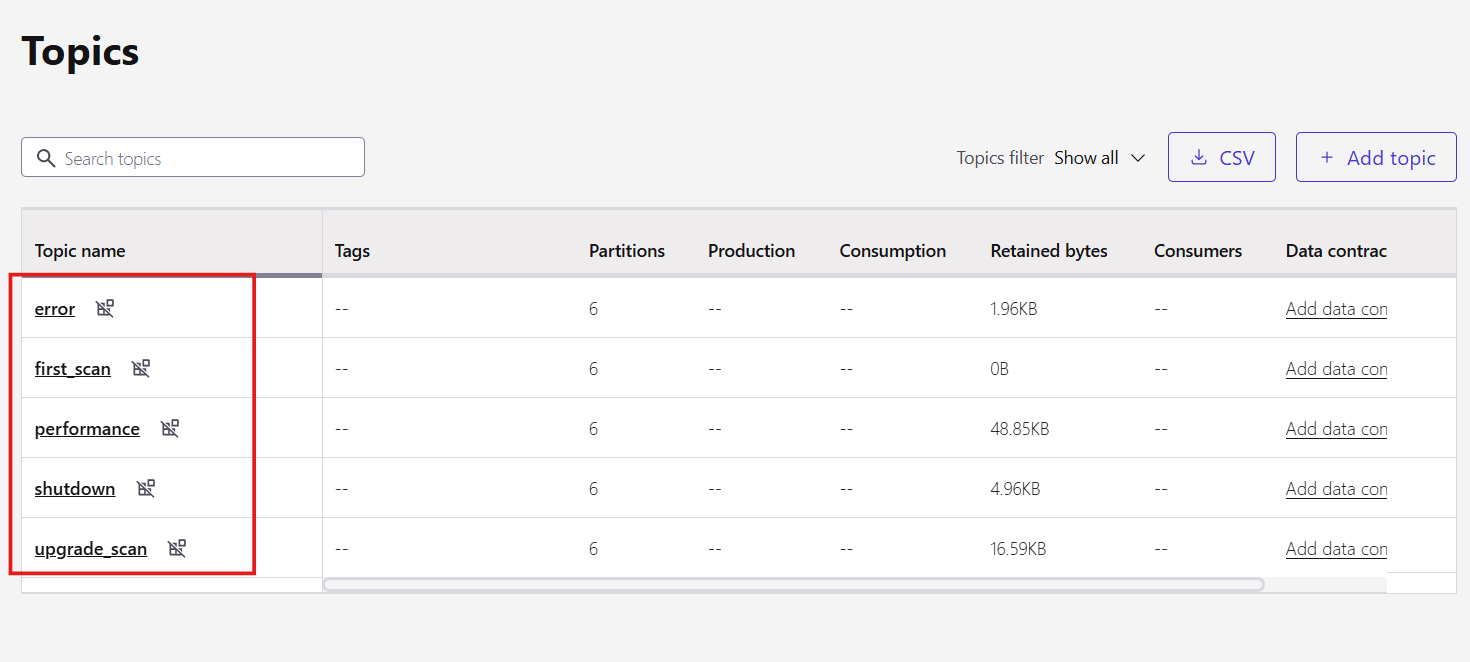
\includegraphics[width=0.9\linewidth]{Images/topic.png}
%     \vspace{10pt}
%     \caption{Topic Config}
%     \label{fig:enter-label}
% \end{figure}
% \noindent Trên Confluent Cloud nhóm đã cài đặt tổng cộng 4 topic cho một cluster phục vụ tương ứng 4 nghiệp vụ khác nhau:
% \begin{itemize}[label=--]
%     \item Performance: Dùng để nhận dữ liệu hiệu suất tài sản từ tool Collector và gửi đến Backend Server.
%     \item First Scan: Dùng để nhận dữ liệu cho các tác vụ quét lần đầu khi triển khai tài sản.
%     \item Upgrade Scan: Dùng để nhận dữ liệu cho các tác vụ quét sau khi nâng cấp, thay thế tài sản.
%     \item Error: Dùng để nhận dữ liệu sự cố, hoặc lỗi của thiết bị. Đối với những lỗi xảy ra nhưng máy tính vẫn hoạt động được (thiếu RAM, thiếu ổ cứng, không có GPU) dữ liệu sẽ gửi qua topic Error. Còn đối với các trường hợp khác khiến máy tắt ngay lập tức hoặc không thể kết nối mạng, nhân viên sử dụng tài sản sẽ báo cáo cho nhân viên IT để tiến hành khắc phục sự cố
% \end{itemize}
% \subsubsection{Cấu hình Topic}
% \noindent Mỗi topic sẽ có các thông tin cấu hình như sau :
% \begin{itemize}[label=--]
%     \item Name: Tên topic
%     \item Partitions: Số lượng partition, nhóm đã cài đặt 6 partition cho mỗi topic, mỗi tầng hoặc mỗi phòng ban của công ty/tổ chức sẽ tương ứng với một partition (có thể mở rộng partition theo như cầu). Mỗi partition sẽ có số lượng offset cực kì lớn.
%     \item Cleanup Policy: Cách dữ liệu được xử lý sau khi đã được tiêu thụ. Ở đây nhóm chọn \textbf{delete} để sau khi tiêu thụ tin nhắn sẽ được xóa sau một khoảng thời gian đã cài đặt trước. Ngược lại có thể chọn \textbf{compact} nếu giữ lại bản ghi mới nhất với cùng key.
%     \item Retention time:  Thời gian lưu giữ bản ghi trên topic (tính bằng milliseconds). Xác định Kafka sẽ giữ dữ liệu bao lâu trước khi xóa, ảnh hưởng đến dung lượng lưu trữ. Nhóm đã cài đặt thời gian là 1 tuần 
%     \item Retention Byte: Dung lượng tối đa mà topic có thể lưu giữ. Nếu đạt đến giới hạn này, Kafka sẽ xóa dữ liệu cũ hơn (nếu cleanup.policy=delete). Ở đây nhóm đã không cài đặt giới hạn số byte cho topic.
%     \item Min Replica: Số replica tối thiểu cần đồng bộ để cho phép ghi. Đảm bảo độ bền dữ liệu. Nếu nhỏ hơn số replica in-sync, producer sẽ gặp lỗi khi ghi từ đó tăng tính an toàn. Nhóm đã cài đặt min replica là 2
%     \item Compression Type: Loại thuật toán nén sử dụng cho dữ liệu gửi lên topic. Giảm dung lượng lưu trữ và băng thông mạng, nhưng có thể làm tăng độ trễ do tốn CPU. Nhóm đã cài đặt là "Producer" tức là cấu hình theo Producer
%     \item Max Message Bytes: Kích thước tối đa của một bản ghi Kafka (message). Nhóm đã cài đặt dung lượng tối đa cho một message là 2MB.

% \end{itemize}
% \subsubsection{Cấu hình Producer}
% \noindent Trong hệ thống quản lý tài sản CNTT thời gian thực, dữ liệu từ các máy trạm người dùng được thu thập bởi một module có tên gọi là Collector. Collector đóng vai trò như một producer gửi thông tin giám sát hiệu suất, phần cứng, phần mềm của máy tính cá nhân đến hệ thống trung tâm thông qua nền tảng Confluent Cloud.\\ \\
% Để kết nối đến Confluent Cloud, Collector cần cấu hình một số thông số bảo mật nhằm đảm bảo kênh truyền dữ liệu được mã hóa và xác thực đầy đủ. Cấu hình Producer như sau:
% \begin{itemize}[label=--]
%     \item \textbf{Bootstrap.servers}: Địa chỉ máy chủ Kafka broker để kết nối ban đầu, sau đó producer sẽ tự động phát hiện các broker khác trong cluster. 
%     Nhóm đã thiết lập đường dẫn là "pkc-l7j7w.asia-east1.gcp.confluent.cloud:9092". Đây là endpoint của Confluent Cloud ở region Asia-East1 (Đài Loan) trên nền tảng GCP.
%     \item \textbf{Security.protocol}: Nhóm đã thiết lập là "SASL\_SSL", tức là Chỉ định sử dụng SASL (Simple Authentication and Security Layer) với SSL để mã hóa kết nối.
%     \item \textbf{SASL Mechanism}: PLAIN , Cơ chế xác thực đơn giản bằng username/password.
%     \item \textbf{SASL Username}: API Key để xác thực với Confluent Cloud.
%     \item \textbf{SASL Password}: API secret tương ứng với key trên.
%     \item \textbf{Client Id}: Định danh duy nhất cho producer, giúp theo dõi và quản lý client.
%     \item \textbf{Retries}: 3 , thử gửi lại tối đa 3 lần khi gặp lỗi mạng.
% \end{itemize}
% \subsubsection{Cấu hình Consumer}
% \noindent Để tiêu thụ dữ liệu từ Kafka trên nền tảng Confluent Cloud, Consumer được thiết lập ở Backend server và được chạy dưới dạng dịch vụ nền (Background Service). Cấu hình Consumer như sau:
% \begin{itemize}[label=--]
%     \item \textbf{BootstrapServers}: Đây là địa chỉ Kafka Broker mà Consumer sẽ kết nối ban đầu. Sau khi kết nối, Consumer sẽ tự động phát hiện các broker khác trong cluster. Nhóm đã cài đặt như ở Producer.
%     \item Các thông số \textbf{Security Protocol}, \textbf{SASL Mechanism} và cả \textbf{Username, password} được cài đặt như ở Producer.
%     \item \textbf{GroupId}: Mỗi Consumer Group có một ID duy nhất để Kafka theo dõi offset (vị trí đọc dữ liệu).
%     \item \textbf{AutoOffsetReset}: Xác định hành vi khi Consumer Group mới hoặc offset không tồn tại. Có hai lựa chọn là Latest (Bắt đầu đọc từ message mới nhất - bỏ qua dữ liệu cũ ) và Earliest (Bắt đầu đọc từ message đầu tiên trong topic), để phù hợp với hệ thống nhóm đã chọn "Latest". Lựa chọn này chỉ quan tâm dữ liệu mới, không cần xử lý dữ liệu cũ. Ngoài ra có thể tránh xử lý lại lượng lớn dữ liệu lịch sử. 
%     \item \textbf{EnableAutoCommit}: Nếu là True, Consumer sẽ tự động commit offset sau khi xử lý message. 
% \end{itemize}

% \subsection{Hiện thực các tính năng}
% \noindent Nhóm tiến hành xây dựng hệ thống web với mục tiêu là cung cấp một giao diện đẹp, trực quan, và dễ sử dụng cho người dùng, đồng thời đáp ứng được các yêu cầu chức năng đã đề cập trước đó.

% \begin{itemize}[label=--]
%     \item Hiện thực tính năng giám sát\\
%     Để truy cập tính năng này, người dùng cần đăng nhập, sau đó bấm vào nút "Bảng giám sát". Giao diện thời gian thực sẽ liên tục cập nhật trạng thái của các máy tính có trong hệ thống, giúp người dùng (nhân viên IT) dễ dàng phát hiện những máy tính cần hỗ trợ (xem thêm ở phụ lục).
%     \begin{figure}[H]
%         \centering
%         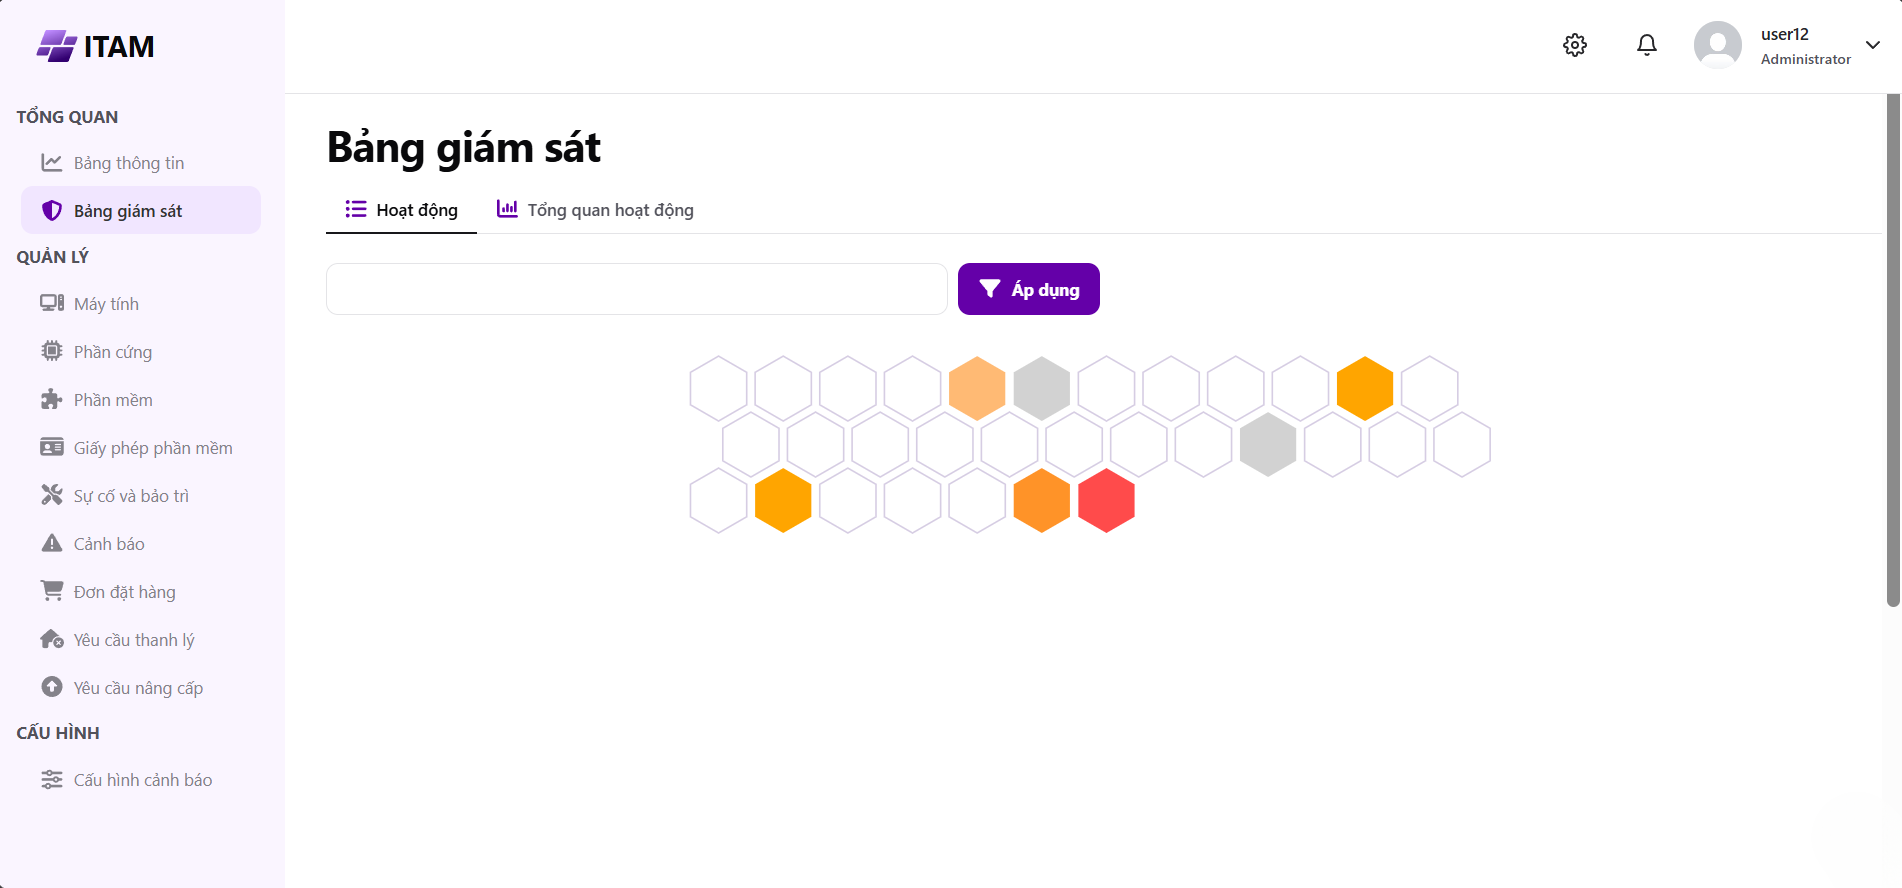
\includegraphics[width=14cm]{Images/C6/UI-Hienthuc/giamsat1.png}
%         \vspace{15pt}
%         \caption{Giao diện hiện thực tính năng Giám sát}
%     \end{figure}

%     \item Hiện thực tính năng quản lý máy tính\\
%     Để truy cập tính năng này, người dùng cần đăng nhập, sau đó bấm vào nút "Máy tính". Ở tính năng này, người dùng có thể thêm thông tin máy tính để quản lý, xem danh sách và chi tiết của máy tính cũng như thông tin vòng đời, hiệu suất, cảnh báo sớm, phần cứng, phần mềm liên quan tới máy tính (xem thêm ở phụ lục).
%     \begin{figure}[H]
%         \centering
%         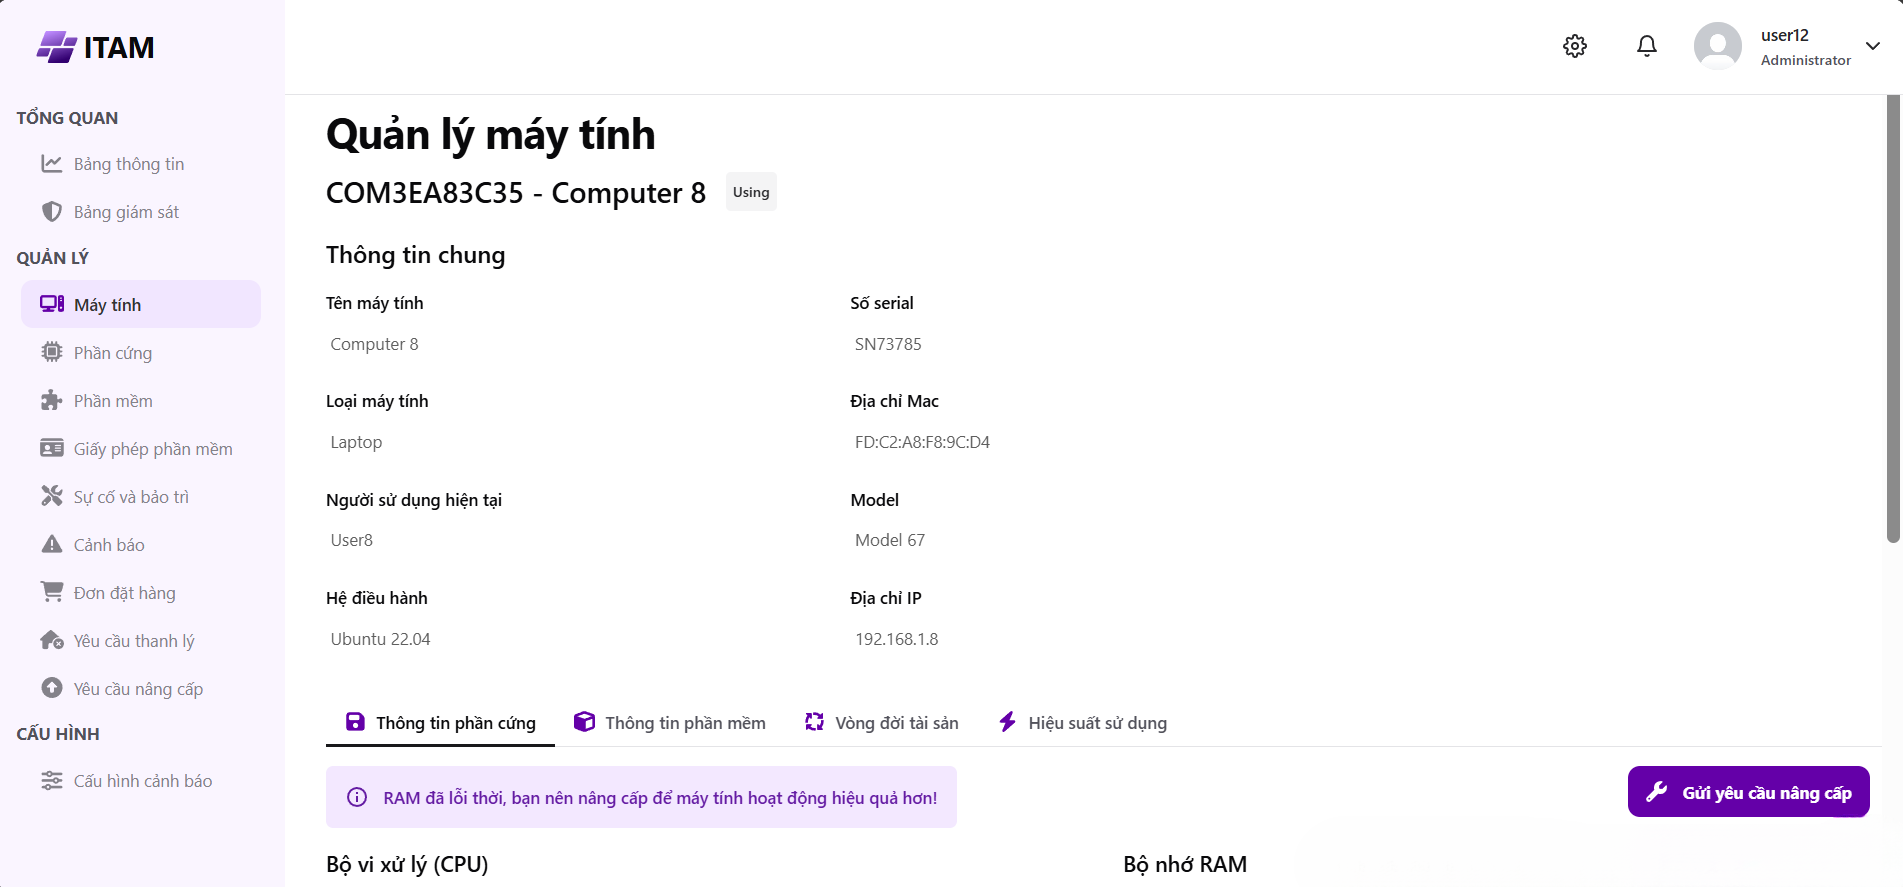
\includegraphics[width=14cm]{Images/C6/UI-Hienthuc/quanlymt1.png}
%         \vspace{15pt}
%         \caption{Giao diện hiện thực tính năng Quản lý máy tính}
%     \end{figure}
%     \begin{figure}[H]
%         \centering
%         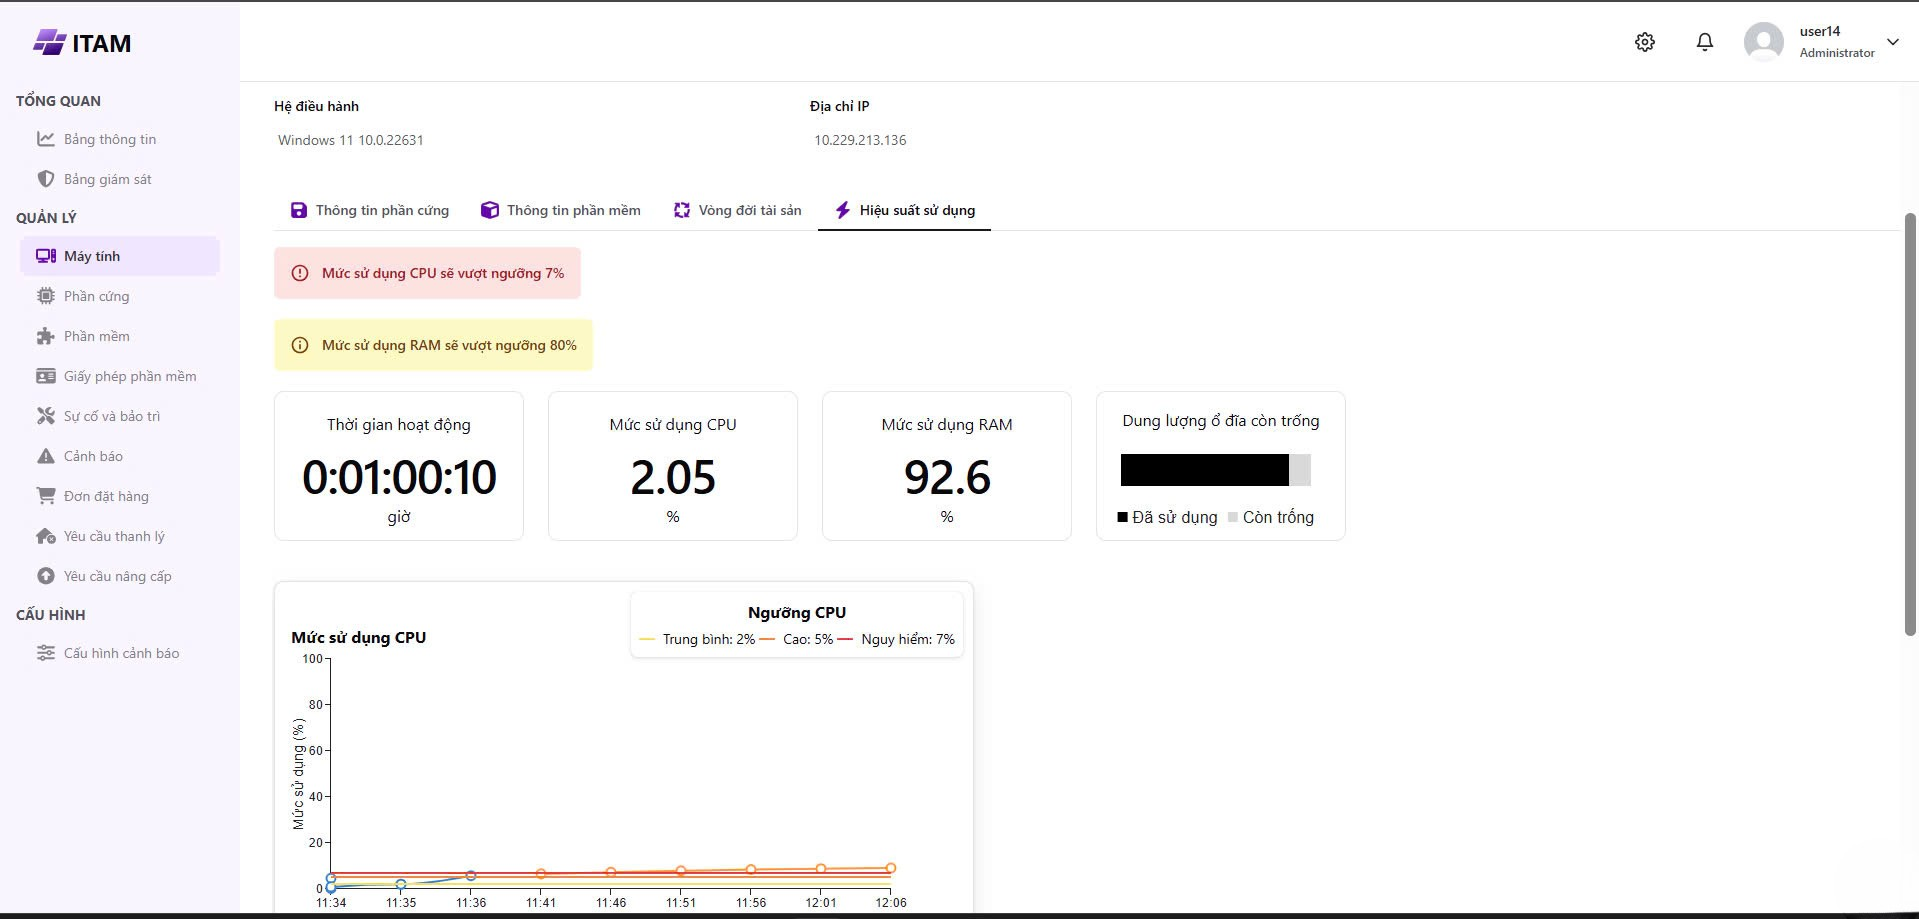
\includegraphics[width=14cm]{Images/C6/UI-Hienthuc/quanlymt3.jpg}
%         \vspace{15pt}
%         \caption{Giao diện hiện thực tính năng Quản lý máy tính - hiệu suất, cảnh báo sớm}
%     \end{figure}

%     \item Hiện thực tính năng Bảng thông tin chung\\
%     Để truy cập tính năng này, người dùng cần đăng nhập, sau đó bấm vào nút "Bảng thông tin". Ở tính năng này, người dùng có thể xem các thông tin chung như tổng giá trị tài sản, tổng yêu cầu nâng cấp bảo trì, đơn đặt hàng (xem thêm ở phụ lục).

%     \item Hiện thực tính năng Quản lý phần cứng, phần mềm\\
%     Để truy cập tính năng này, người dùng cần đăng nhập, sau đó bấm vào nút "Phần cứng" hoặc "Phần mềm". Ở các tính năng này, người dùng có thể xem, chỉnh sửa thông tin về phần cứng, phần mềm, vòng đời của phần cứng, phần mềm và thêm phần cứng, phần mềm vào hệ thống (xem thêm ở phụ lục).

%     \item Hiện thực tính năng Quản lý Giấy phép phần mềm\\
%     Để truy cập tính năng này, người dùng cần đăng nhập, sau đó bấm vào nút "Giấy phép phần mềm". Ở các tính năng này, người dùng có thể xem, chỉnh sửa thông tin giấy phép phần mềm (xem thêm ở phụ lục).

%     \item Hiện thực tính năng Quản lý Sự cố và bảo trì\\
%     Để truy cập tính năng này, người dùng cần đăng nhập, sau đó bấm vào nút "Sự cố và bảo trì". Ở các tính năng này, nhân viên IT có thể xem thông tin sự cố và bảo trì, xác nhận sử lý sự cố và hoàn thành bảo trì (xem thêm ở phụ lục).

%     \item Hiện thực tính năng Quản lý Cảnh báo\\
%     Để truy cập tính năng này, người dùng cần đăng nhập, sau đó bấm vào nút "Cảnh báo". Ở các tính năng này, nhân viên IT có thể dễ dàng xem thông tin của tất cả cảnh báo để có thể ra quyết định xử lý kịp thời (xem thêm ở phụ lục).

%     \item Hiện thực tính năng Quản lý Đơn đặt hàng\\
%     Để truy cập tính năng này, người dùng cần đăng nhập, sau đó bấm vào nút "Đơn đặt hàng". Ở các tính năng này, người quản lý, nhân viên IT có thể xem thông tin đơn hàng. Người quản lý có thể tạo đơn mới hoặc nhập đơn hàng (xem thêm ở phụ lục).

%     \item Hiện thực tính năng Quản lý Yêu cầu nâng cấp, Yêu cầu thanh lý\\
%     Để truy cập tính năng này, người dùng cần đăng nhập, sau đó bấm vào nút "Yêu cầu nâng cấp" hoặc "Yêu cầu thanh lý". Ở các tính năng này, người dùng có thể xem thông tin của tất cả yêu cầu nâng cấp và thanh lý. Người quản lý có thể tiến hành phê duyệt các yêu cầu này (xem thêm ở phụ lục).

%     \item Hiện thực tính năng Cấu hình cảnh báo\\
%     Để truy cập tính năng này, người dùng cần đăng nhập, sau đó bấm vào nút "Cấu hình cảnh báo". Nhân viên IT có thể cấu hình các ngưỡng cảnh báo cho hệ thống (xem thêm ở phụ lục).

%     \item Hiện thực tính năng Báo cáo tổng quan\\
%     Hệ thống còn cung cấp tính năng báo cáo tổng quan như tổng quan về máy tính, phần cứng, phần mềm,... Cung cấp các thông tin tổng quan về số lượng, tình trạng sử dụng, giá trị tài sản,... (xem thêm ở phụ lục).
    
% \end{itemize}

% \subsection{Kiểm thử}
% \noindent Kiểm thử là một giai đoạn quan trọng và không thể thiếu trong quá trình phát triển phần mềm. Nó giúp nhóm phát hiện sớm các lỗi để khắc phục kịp thời, đảm bảo phần mềm hoạt động chính xác, đúng với yêu cầu đặt ra. Dưới đây là kiểm thử cho module giám sát tài sản.
% \subsubsection{Mô tả}
% \noindent Nhóm Giám sát Tài sản tập trung vào việc thu thập và quản lý các thông tin liên quan đến tài sản công nghệ trong hệ thống. Điều này bao gồm việc theo dõi trạng thái, vị trí, tình trạng sử dụng và các thuộc tính khác của tài sản. Mục tiêu chính là giúp tổ chức có cái nhìn toàn diện về tài sản của mình, từ đó tối ưu hóa quản lý và sử dụng.
% \subsubsection{Các bảng dữ liệu liên quan}
% \begin{longtable}{|p{4cm}|p{10cm}|}
%     \caption{Bảng dữ liệu liên quan} \\
%     \hline
%     \textbf{Tên bảng} & \textbf{Mô tả} \\
%     \hline
%     \endfirsthead

%     \hline
%     \textbf{Tên bảng} & \textbf{Mô tả} \\
%     \hline
%     \endhead

%     Asset & Quản lý thông tin chung về tài sản \\
%     \hline
%     Maintenance & Quản lý lịch sử bảo trì của tài sản \\
%     \hline
%     Alert & Ghi nhận các cảnh báo liên quan đến hiệu suất để kịp thời xử lý sự cố. \\
%     \hline
%     AvgPerformance & Lưu trữ dữ liệu hiệu suất trung bình của các thiết bị để phục vụ việc đánh giá và tối ưu sử dụng. \\
%     \hline
%     Lifecycle & Quản lý vòng đời tài sản (Procurement, Implementation, Utilization, Disposal) \\
%     \hline        
% \end{longtable}


% \subsubsection{Các kịch bản kiểm tra}
% \newpage
% \begin{longtable}{
%     |>{\raggedright\arraybackslash}p{0.05\textwidth}
%     |>{\raggedright\arraybackslash}p{0.15\textwidth}
%     |>{\raggedright\arraybackslash}p{0.2\textwidth}
%     |>{\raggedright\arraybackslash}p{0.3\textwidth}
%     |>{\raggedright\arraybackslash}p{0.2\textwidth}|
% }
%     \caption{Các kịch bản kiểm tra} \\
%     \hline
%     \textbf{ID} & \textbf{Testcase} & \textbf{Description} & \textbf{Step} & \textbf{Kết quả} \\
%     \hline
%     % \vspace{0.1pt} A01 &\vspace{0.1pt} Tạo mới tài sản máy tính (vai trò ITStaff, Admin) & \vspace{0.1pt} Người dùng với vai trò ITStaff hoặc Admin tạo mới một tài sản máy tính thông qua giao diện web & 
%     % \begin{itemize}[leftmargin=*,nosep,topsep=0pt,itemsep=0pt]
%     %     \item Log into the website with an Admin or ITStaff account
%     %     \item Click on "Máy tính"
%     %     \item Click on "Thêm máy tính"
%     %     \item Click on "Tên máy tính"
%     %     \item Enter "Test Computer" into "Tên máy tính"
%     %     \item Click on "Loại máy tính"
%     %     \item Enter "Laptop" into "Loại máy tính"
%     %     \item Click on "Model"
%     %     \item Enter "Model 21" into "Model"
%     %     \item Click on "Số serial"
%     %     \item Enter "SN30265" into "Số serial"
%     %     \item Click on "Hệ điều hành"
%     %     \item Enter "Ubuntu 22.04" into "Hệ điều hành"
%     %     \item Click on "Lưu"
%     %     \item Click on "Search..."
%     %     \item Enter "Test Computer" into "Search..."
%     % \end{itemize} &
%     % \begin{itemize}[leftmargin=*,topsep=0pt,itemsep=0pt]
%     %     \item Dữ liệu tài sản được lưu thành công
%     %     \item Hiển thị đúng tài sản khi tìm kiếm
%     % \end{itemize} \\
%     % \hline    
%     \vspace{0.1pt} A01 & \vspace{0.1pt} Kiểm tra quyền hạn tạo tài sản (vai trò Manager) & \vspace{0.1pt} Người dùng với vai trò Manager không được phép tạo tài sản máy tính & 
%     \begin{itemize}[leftmargin=*,topsep=0pt,itemsep=0pt,label=--]
%         \item Log into the website with a Manager account
%         \item Click on "Máy tính"
%     \end{itemize} &
%     \begin{itemize}[leftmargin=*,topsep=0pt,itemsep=0pt,label=--]
%         \item Không hiển thị nút "Thêm máy tính"
%         \item Người dùng không có quyền tạo mới tài sản
%     \end{itemize} \\
%     \hline    
%     \vspace{0.1pt} A02 & \vspace{0.1pt} Cập nhật chi tiết tài sản máy tính & \vspace{0.1pt} Cập nhật thông tin tài sản như tên máy tính, người sử dụng hiện tại, địa chỉ IP & 
%     \begin{itemize}[leftmargin=*,topsep=0pt,itemsep=0pt,label=--]
%         \item Log into the website with an Administrator or ITStaff account
%         \item Click on "Máy tính"
%         \item Click on "COM00659887"
%         \item Click on "editable input"
%         \item Enter "Computer 66" into "editable input"
%         \item Reload
%     \end{itemize} &
%     \begin{itemize}[leftmargin=*,topsep=0pt,itemsep=0pt,label=--]
%         \item Thông tin cập nhật được lưu thành công
%         \item Hiển thị đúng thông tin sau khi reload
%     \end{itemize} \\
%     \hline
%     \vspace{0.1pt} A03 & \vspace{0.1pt} Kiểm tra quyền hạn chỉnh sửa tài sản (vai trò Manager) & \vspace{0.1pt} Người dùng với vai trò Manager không được phép chỉnh sửa tài sản & 
%     \begin{itemize}[leftmargin=*,topsep=0pt,itemsep=0pt,label=--]
%         \item Log into the website with a Manager account
%         \item Click on "Máy tính"
%         \item Click on "COM00659887"
%         \item Click on "Computer 6"
%     \end{itemize} &
%     \begin{itemize}[leftmargin=*,topsep=0pt,itemsep=0pt,label=--]
%         \item Không thể chỉnh sửa các input field
%     \end{itemize} \\
%     \hline    
%     \vspace{0.1pt} A04 & \vspace{0.1pt} Thông tin phần cứng của máy tính & \vspace{0.1pt} Kiểm tra hệ thống hiển thị đúng thông tin phần cứng của máy tính & 
%     \begin{itemize}[leftmargin=*,topsep=0pt,itemsep=0pt,label=--]
%         \item Log into website
%         \item Click on "Máy tính"
%         \item Click on "COM00659887"
%         \item Click on "Thông tin phần cứng"
%     \end{itemize} &
%     \begin{itemize}[leftmargin=*,topsep=0pt,itemsep=0pt,label=--]
%         \item Hiển thị đúng thông tin CPU, RAM, ổ cứng, card mạng, GPU
%     \end{itemize} \\
%     \hline    
%     \vspace{0.1pt} A05 & \vspace{0.1pt} Thông tin phần mềm của máy tính & \vspace{0.1pt} Kiểm tra hệ thống hiển thị đúng danh sách phần mềm đã cài đặt & 
%     \begin{itemize}[leftmargin=*,topsep=0pt,itemsep=0pt,label=--]
%         \item Log into website
%         \item Click on "Máy tính"
%         \item Click on "COM00659887"
%         \item Click on "Thông tin phần mềm"
%     \end{itemize} &
%     \begin{itemize}[leftmargin=*,topsep=0pt,itemsep=0pt,label=--]
%         \item Hiển thị đầy đủ danh sách phần mềm
%         \item Bao gồm tên, phiên bản, nhà phát hành
%     \end{itemize} \\
%     \hline    
%     \vspace{0.1pt} A06 & \vspace{0.1pt} Hiệu suất sử dụng máy tính & \vspace{0.1pt} Kiểm tra tính năng theo dõi hiệu suất hoạt động & 
%     \begin{itemize}[leftmargin=*,topsep=0pt,itemsep=0pt,label=--]
%         \item Log into website
%         \item Click on "Máy tính"
%         \item Click on "COM0AF0C218"
%         \item Click on "Hiệu suất sử dụng"
%     \end{itemize} &
%     \begin{itemize}[leftmargin=*,topsep=0pt,itemsep=0pt,label=--]
%         \item Hiển thị bảng theo dõi hiệu suất CPU, RAM, ổ đĩa
%     \end{itemize} \\
%     \hline
    
%     \vspace{0.1pt} A07 & \vspace{0.1pt} Báo cáo tổng quan máy tính & \vspace{0.1pt} Kiểm tra hệ thống hiển thị báo cáo tổng quan & 
%     \begin{itemize}[leftmargin=*,topsep=0pt,itemsep=0pt,label=--]
%         \item Log into website
%         \item Click on "Máy tính"
%         \item Click on "Báo cáo tổng quan"
%     \end{itemize} & 
%     \begin{itemize}[leftmargin=*,topsep=0pt,itemsep=0pt,label=--]
%         \item Hiển thị số lượng máy tính theo loại
%         \item Hiển thị tình trạng sử dụng
%     \end{itemize} \\
%     \hline    
%     \vspace{0.1pt} A08 & \vspace{0.1pt} Bảng giám sát hoạt động & \vspace{0.1pt} Đảm bảo bảng giám sát hiển thị đúng lỗi và cảnh báo & 
%     \begin{itemize}[leftmargin=*,topsep=0pt,itemsep=0pt,label=--]
%         \item Log into website
%         \item Click on "Bảng giám sát"
%         \item Xem thông tin giám sát của một máy tính
%         \item Kiểm tra cảnh báo hiệu suất
%     \end{itemize} &
%     \begin{itemize}[leftmargin=*,topsep=0pt,itemsep=0pt,label=--]
%         \item Hiển thị realtime các hoạt động
%         \item Cảnh báo khi vượt ngưỡng
%     \end{itemize} \\
%     \hline
%     \vspace{0.1pt} A9 & \vspace{0.1pt} Tổng quan hoạt động tài sản & \vspace{0.1pt} Xác minh giao diện báo cáo tổng hợp tình trạng lỗi & 
%     \begin{itemize}[leftmargin=*,topsep=0pt,itemsep=0pt,label=--]
%         \item Log into website
%         \item Click on "Bảng giám sát"
%         \item Click on "Tổng quan hoạt động"
%     \end{itemize} &
%     \begin{itemize}[leftmargin=*,topsep=0pt,itemsep=0pt,label=--]
%         \item Hiển thị tổng quan tình trạng sử dụng
%         \item Thống kê theo phòng ban, địa điểm
%     \end{itemize} \\
%     \hline
% \end{longtable}
% \noindent Và đó là phần kiểm thử cho module giám sát tài sản của hệ thống. Ngoài ra, nhóm đã thiết kế tổng cộng 6 nhóm testcases tương ứng với các module của hệ thống lần lượt là Quản lý người dùng, Thu thập và quản lý tài sản (Giám sát tài sản), Quản lý vòng đời tài sản; Cấu hình cảnh báo và cảnh báo; Bảo trì và lỗi; Quản lý nhà cung cấp và đơn đặt hàng. Kiểm thử đầy đủ được trình bày tại đây \href{https://docs.google.com/spreadsheets/d/1jniVzouwGwiA-Zut57mP8WkhuAvEHiyQ/edit?usp=sharing&ouid=113898029022770865736&rtpof=true&sd=true}{Link}.
% \subsection{Sử dụng LSTM cho dự đoán hiệu suất sử dụng CPU, RAM}
% \begin{enumerate}
%     \item \textbf{Mô tả dữ liệu}\\ \href{https://drive.google.com/file/d/1M5THsCWqN3WJ1JGntOy3PdtKMNtWeUR1/view?usp=sharing}{Đường link của dữ liệu}\\
%     Dữ liệu được thu thập từ máy của các người dùng khác nhau, liên tục và cách quãng nhau 10 phút. Dữ liệu dùng để huấn luyện có các thông tin như sau:
%     \begin{itemize}[label=--]
%         \item Thông tin CPU: 
%         \begin{itemize}[label=\textbullet]
%             \item Mức độ sử dụng (utilization): Là nhãn trong bài toán dự đoán CPU 
%             \item Số lượng tiến trình đang hoạt động (processes): Góp phần quyết định mức sử dụng CPU và bộ nhớ
%             \item Thời gian hoạt động liên tục (uptime) tính từ thời điểm restart máy đến hiện tại: Càng hoạt động lâu, hệ thống có xu hướng tiêu tốn tài nguyên nhiều hơn
%         \end{itemize}
%         \item Thông tin RAM: tỷ lệ bộ nhớ đang sử dụng (percent).
%         \item Thông tin ổ đĩa: tổng bộ nhớ đã sử dụng (total\_memory\_used), tỷ lệ bộ nhớ đã dùng (percent\_mem\_used).
%         \item Thông tin mạng: tốc độ card mạng (inet\_card\_speed).
%         \item Thông tin hệ thống: thời gian khởi động hệ điều hành (boot\_time), thời gian quét (scantime), vị trí máy (location), và người dùng hiện tại (currentUser). 
%         \item Thông tin về giờ làm việc: thời gian thu thập có phải trong giờ làm việc hay không.
%         \item Ngày trong tuần: ngày thu thập dữ liệu có phải ngày trong tuần không. Nhận biết xu hướng hoạt động theo thời gian làm việc – ví dụ: cao điểm thứ 2-6
%     \end{itemize}
%     Dữ liệu sau khi thu thập được tiền xử lý và lưu vào định dạng CSV để phục vụ cho việc huấn luyện. \\
%     Quá trình tiền xử lý bao gồm: 
%     \begin{itemize}[label=--]
%         \item Xử lý các giá trị bị null và outlier
%         \item Chuyển đổi định dạng thời gian
%         \item Chuẩn hóa dữ liệu đầu vào và đầu ra bằng MinMaxScaler
%     \end{itemize}
%     Sau đó, dữ liệu được gom lại theo chuỗi thời gian, đảm bảo khoảng cách thời gian dữ liệu không quá 20 phút. Sau khi nhóm thành các nhóm nhỏ thì sẽ gộp các chuỗi lại theo CPU riêng và Ram Riêng.
%     \item \textbf{Cấu trúc mô hình LSTM}\\
%     Mô hình dự báo được xây dựng dựa trên kiến trúc Long Short-Term Memory (LSTM) – một biến thể của mạng nơ-ron hồi quy (RNN) chuyên biệt cho xử lý chuỗi thời gian và dữ liệu có tính tuần tự.\\
%     Cấu trúc chi tiết của mô hình như sau:
%     \begin{enumerate}
%         \item \textbf{Lớp LSTM thứ nhất (64 units)}:\\
%         Lớp đầu (return\_sequences=True) trả về chuỗi đầy đủ để lớp thứ hai có thể xử lý thông tin thời gian đa tầng.
%         \begin{itemize}[label=--]
%             \item \textbf{Lựa chọn Activation Functions}: 
%             \begin{itemize}[label=\textbullet]
%                 \item \textbf{tanh} cho trạng thái cell: Giới hạn đầu ra trong khoảng [-1, 1], tránh bùng nổ giá trị.
%                 \item \textbf{sigmoid} cho các cổng (input/forget/output gates): Đưa giá trị về [0, 1], phù hợp cho việc điều khiển tỷ lệ thông tin được giữ/loại bỏ.
%             \end{itemize}
%             \item \textbf{Regularization (L1/L2)}: $l=1e-5$, $l2=1e-4$: Áp dụng regularization để phạt trọng số lớn, ngăn chặn overfitting. L2 (Ridge) thường hiệu quả hơn L1 (Lasso) với RNN do tính chất của dữ liệu chuỗi thời gian.
%             \item \textbf{Batch Normalization (BatchNorm)}: Chuẩn hóa đầu ra sau mỗi lớp LSTM để ổn định phân phối dữ liệu qua các lớp, giảm hiện tượng "internal covariate shift", giúp mô hình hội tụ nhanh hơn.
%             \item \textbf{Dropout 30\%}: Tỷ lệ cao hơn so với thông thường (20\%) do LSTM dễ overfitting với dữ liệu nhỏ. Dropout ngẫu nhiên loại bỏ 30\% units trong quá trình huấn luyện để tăng tính tổng quát.
%         \end{itemize}
%         \item \textbf{Lớp LSTM thứ hai (32 units)}:
%         \begin{itemize}[label=--]
%             \item \textbf{Giảm số units (64 → 32)}: Lớp sau cần ít units hơn do đã trích xuất features quan trọng từ lớp trước. Việc giảm số units giúp giảm tham số, tránh overfitting.
%             \item \textbf{return\_sequences=False}: Chỉ trả về đầu ra cuối cùng (không cần chuỗi) vì bài toán là regression (dự đoán giá trị đơn).
%         \end{itemize}
%         \item \textbf{Lớp Dense trung gian (32 units)}
%         \begin{itemize}[label=--]
%             \item Lớp Dense với ReLU (Rectified Linear Unit) giúp kết hợp phi tuyến tính các features từ LSTM trước khi đưa ra kết quả. ReLU được chọn do tính đơn giản và hiệu quả với dữ liệu không âm.
%             \item Lớp đầu ra (linear): Activation linear phù hợp cho regression vì không giới hạn khoảng giá trị đầu ra.
%         \end{itemize}
%         \item \textbf{Cấu hình huấn luyện}:
%         \begin{itemize}[label=--]
%             \item Adam: Kết hợp ưu điểm của RMSProp và Momentum, tự động điều chỉnh learning rate cho từng trọng số. Hiệu quả với dữ liệu chuỗi thời gian do khả năng xử lý nhiễu.
%             \item Learning rate 0.001: Giá trị phổ biến để cân bằng giữa tốc độ hội tụ và ổn định. Nếu quá lớn, mô hình có thể phân kỳ; quá nhỏ dẫn đến hội tụ chậm.
%             \item Gradient Clipping (clipvalue=0.5): Cắt gradient nếu vượt quá 0.5 để tránh hiện tượng "gradient explosion" (phổ biến ở RNN do tích luỹ gradient qua các bước thời gian).
%             \item Hàm mất mát (loss function): Mean Squared Error (MSE) – phù hợp với bài toán hồi quy liên tục.
%         \end{itemize}
%     \end{enumerate}
%     \item \textbf{Quá trình huấn luyện}\\
%     Mô hình được huấn luyện bằng phương pháp học có giám sát với thông số cấu hình như sau:
%     \begin{itemize}[label=--]
%         \item Số lượng epoch: 100
%         \item Kích thước batch: 32
%         \item Sử dụng kỹ thuật Early Stopping để tự động dừng quá trình huấn luyện khi sai số trên tập kiểm tra không còn giảm sau 10 epoch liên tiếp, đồng thời khôi phục lại trọng số tốt nhất.
%     \end{itemize}
%     Dữ liệu đầu vào có định dạng ba chiều [samples, time steps, features], tương ứng với các đặc trưng đã được chuẩn hóa từ dữ liệu gốc. Kết quả huấn luyện được lưu lại để phục vụ đánh giá và trực quan hóa.
%     \item \textbf{Đánh giá mô hình}:\\
%     Sau quá trình huấn luyện, mô hình được đánh giá trên tập kiểm tra thông qua hàm evaluate() để tính toán giá trị sai số trung bình bình phương (MSE). Ngoài ra, kết quả dự đoán cũng được chuyển đổi ngược trở lại giá trị ban đầu thông qua inverse\_transform nhằm so sánh trực tiếp với giá trị thực tế.
%     Kết quả đạt được:
%     \begin{itemize}[label=--]
%         \item CPU - MAE: 3.73, CPU - RMSE: 5.16
%         \item RAM - MAE: 3.51, RAM - RMSE: 5.73
%         \item CPU Loss: 25.58
%         \item RAM Loss: 32.85
%     \end{itemize}
%     \textbf{Nhận xét}: Kết quả cho thấy mô hình đạt độ chính xác tương đối tốt với cả hai đầu ra là mức sử dụng CPU và RAM. Sai số trung bình tuyệt đối (MAE) đều dưới 4\%, cho thấy dự đoán gần với giá trị thực tế. RMSE và Loss cho RAM cao hơn một chút so với CPU, điều này có thể phản ánh sự dao động lớn hơn hoặc tính khó dự đoán hơn của mức sử dụng RAM theo thời gian. Tuy nhiên, các chỉ số vẫn nằm trong phạm vi chấp nhận được cho các bài toán dự đoán tài nguyên hệ thống trong thực tế.
%     Nhìn chung, mô hình có khả năng dự báo hiệu quả hiệu suất hệ thống trong ngắn hạn, giúp hỗ trợ đưa ra cảnh báo sớm đối với thiết bị.\\ \\
%     Bên cạnh sử dụng mô hình LSTM nhóm cũng đã sử dụng hai mô hình tương tác tốt với dữ liệu tuần tự theo thời gian là RNN (Recurrent Neural Network) thường và GRU (Gated Recurrent Unit).\\
% \noindent Bảng tổng hợp kết quả thu được như sau:
% \begin{longtable}{|p{0.1\textwidth}|p{0.1\textwidth}|p{0.1\textwidth}|p{0.1\textwidth}|p{0.1\textwidth}|p{0.1\textwidth}|p{0.1\textwidth}|}
%     \caption{Tổng hợp kết quả thực nghiệm trên GRU, RNN, LSTM}\\
%     \hline
%     \textbf{Mô hình}  & \textbf{CPU MAE} & \textbf{CPU RMSE} & \textbf{CPU Loss} & \textbf{RAM MAE}& \textbf{RAM RMSE} & \textbf{RAM Loss} \\
%    \hline
%     \textbf{LSTM} & 3.73 & 5.06 & 25.58 & 3.51 & 5.73 & 32.85 \\
%     \hline
%     \textbf{RNN}  & 3.85 & 5.37 & 30.28 & 3.89 & 5.96 & 34.31 \\
%     \hline
%     \textbf{GRU}  & 3.75 & 5.09 & 25.71 & 4.30 & 6.16 & 37.93 \\
%     \hline
% \end{longtable}
% Dựa trên bảng kết quả thực nghiệm, có thể thấy mô hình LSTM đạt hiệu suất tương đối tốt trên hầu hết các chỉ số đánh giá. Cụ thể, LSTM cho giá trị sai số tuyệt đối trung bình (MAE) và sai số bình phương trung bình (RMSE) thấp nhất đối với cả CPU và RAM, lần lượt là CPU MAE = 3.73, CPU RMSE = 5.06, RAM MAE = 3.51, và RAM RMSE = 5.73. Mặc dù GRU có CPU Loss thấp hơn một chút (25.71 so với 25.58 của LSTM), nhưng nhìn chung LSTM vẫn cho thấy sự ổn định và chính xác hơn trên toàn bộ các chỉ số.

% Lý do nhóm lựa chọn LSTM thay vì RNN hoặc GRU là vì LSTM có khả năng ghi nhớ các mối quan hệ dài hạn trong chuỗi thời gian tốt hơn, điều này rất quan trọng trong việc dự đoán hiệu suất tài nguyên như CPU và RAM—vốn phụ thuộc nhiều vào xu hướng sử dụng trong quá khứ. RNN đơn giản thường gặp vấn đề về mất thông tin ở chuỗi dài (vanishing gradient), còn GRU tuy nhẹ hơn nhưng trong thử nghiệm thực tế của nhóm lại cho kết quả kém ổn định hơn so với LSTM. Do đó, LSTM được lựa chọn làm mô hình chính trong hệ thống dự đoán hiệu suất tài sản IT.

% \end{enumerate}

% \subsection{Kết chương}
% Phần kiểm thử được xây dựng trên các kịch bản kiểm tra cụ thể, bám sát các yêu cầu chức năng của từng module. Các trường hợp kiểm thử (testcase) được trình bày rõ ràng với đầu vào, kỳ vọng và kết quả bao gồm các hoạt động như:
% \begin{itemize}[label=--]
%     \item Thêm mới tài sản, phần cứng, phần mềm.
%     \item Cập nhật thông tin và liên kết tài sản với các thực thể liên quan.
%     \item Truy vấn dữ liệu tài sản, bảo trì, lịch sử thay đổi và các thông tin liên quan khác.
%     \item Xóa dữ liệu và kiểm tra liên kết giữa các bảng.
% \end{itemize}
% Nhóm đã thiết kế tổng cộng 6 nhóm kiểm thử, đảm bảo toàn bộ các module chính của hệ thống được kiểm tra đầy đủ và kỹ lưỡng. Điều này không chỉ giúp phát hiện và sửa lỗi trong giai đoạn phát triển mà còn đảm bảo hệ thống hoạt động đúng theo yêu cầu đặt ra. \\ \\
% Ngoài ra, hệ thống còn tích hợp mô hình LSTM (Long Short-Term Memory) nhằm dự đoán hiệu suất sử dụng CPU và RAM của các tài sản theo thời gian. Mô hình được triển khai thông qua một API sử dụng FastAPI, cho phép backend gửi dữ liệu đầu vào và nhận kết quả dự đoán theo yêu cầu.\\ \\
% Nhìn chung, việc hiện thực, kiểm thử và tích hợp trí tuệ nhân tạo đã đặt nền tảng vững chắc cho hệ thống quản lý tài sản CNTT thời gian thực, đảm bảo tính hiệu quả, mở rộng và khả năng thích ứng với các nhu cầu phát triển trong tương lai.

% \newpage
% \section{Đánh giá hệ thống}
\noindent Hệ thống sử dụng Apache Kafka trên Confluent Cloud để thực hiện thu thập dữ liệu thời gian thực từ các thiết bị tài sản công nghệ thông tin, bao gồm phần cứng và phần mềm. Thành phần Kafka Producer được triển khai trên các thiết bị đầu cuối để đẩy dữ liệu lên Kafka Cluster, trong đó mỗi sự kiện hoặc thông tin liên quan đến tài sản (như trạng thái hoạt động, lỗi phát sinh, hiệu năng) được gửi dưới dạng thông điệp (message). \\ \\
Kafka Producer: Gửi thông điệp từ các thiết bị IT Users lên Kafka Cluster.
Kafka Broker: Tiếp nhận và lưu trữ tạm thời thông điệp, chờ các dịch vụ tiêu thụ.
Consumer: Các thành phần như Asset Monitoring Service và Alert \& Notification Service tiêu thụ dữ liệu để thực hiện phân tích và đưa ra các cảnh báo.
\subsection{Đánh giá hiệu năng thu thập dữ liệu thời gian thực với Kafka}
\noindent Đánh giá hiệu năng Kafka qua \textit{kafka-producer-perf-test} và \textit{kafka-consumer-perf-test} mà Kafka hỗ trợ.\\ \\
Với mục tiêu đề tài là thiết kế hệ thống cho đối tượng công ty vừa và nhỏ, với số lượng máy tính nằm trong khoảng 50 - 100, nhóm đã thực hiện đánh giá qua giả lập như sau (bỏ qua độ trễ của môi trường mạng):
\begin{enumerate}
    \item \textbf{Producer}\\
        \textbf{Mục tiêu}: Đánh giá hiệu năng của Kafka Producer dựa trên các chỉ số tốc độ gửi (MB/sec), độ trễ trung bình (ms) và độ trễ lớn nhất (ms) với các kích thước gói tin và số lượng máy tính khác nhau.\\
        Phương pháp: 
        \begin{longtable}{|p{0.1\textwidth}|p{0.12\textwidth}|p{0.2\textwidth}|p{0.2\textwidth}|p{0.2\textwidth}|}
            \caption{Đánh giá Producer}\\
            \hline
            \textbf{Số lượng máy tính} & \textbf{Kích thước gói tin (byte)} & \textbf{Tốc độ gửi (MB.sec)} & \textbf{Độ trễ trung bình (ms)} & \textbf{Độ trễ lớn nhất (ms)} \\
            \hline
            5 & 20000 & 0.27 & 75 & 302\\
            \hline
            25 & 20000 & 1.41 & 46.96 & 301\\
            \hline
            50 & 20000 & 1.78 & 54.78 & 308\\
            \hline
            75 & 20000 & 3.41 & 59.31 & 346\\
            \hline
            100 & 20000 & 4.7 & 68.76 & 425\\
            \hline
            125 & 20000 & 5.51 & 69.17 & 453\\
            \hline
             5 & 50000 & 0.35 & 93 & 313\\
            \hline
            25 & 50000 & 1.41 & 46.96 & 301\\
            \hline
            50 & 50000 & 3.52 & 45 & 298\\
            \hline
            100 & 50000 & 11.66 & 48.05 & 330\\
            \hline
            125 & 50000 & 14.33 & 65.67 & 332\\
            \hline
        \end{longtable}
        \begin{itemize}[label=--]
            \item  Ảnh hưởng của số lượng máy tính: Nhìn chung, tốc độ gửi tăng khi số lượng máy tính, mỗi máy tính tương ứng với một gói tin. Điều này cho thấy Producer có khả năng xử lý hiệu quả lượng lớn tin nhắn. Tuy nhiên, độ trễ trung bình và độ trễ lớn nhất cũng có xu hướng tăng, đặc biệt khi số lượng record vượt quá 100.
            \item Ảnh hưởng của kích thước gói tin: Khi tăng kích thước gói tin từ 20000 byte lên 50000 byte (với 50 record), tốc độ gửi tăng đáng kể (từ 1.78 MB/sec lên 3.52 MB/sec) trong khi độ trễ trung bình giảm. Điều này cho thấy Producer có thể xử lý các record lớn một cách hiệu quả.
            \item Độ trễ: Độ trễ trung bình dao động trong khoảng 45 ms đến 93 ms, cho thấy Producer gửi tin nhắn với độ trễ tương đối thấp. Tuy nhiên, độ trễ lớn nhất có thể lên đến 453 ms, cho thấy có sự không đồng đều về độ trễ giữa các tin nhắn.
        \end{itemize}
        => \textbf{Kafka Producer} cho thấy hiệu năng tốt với khả năng xử lý lượng lớn tin nhắn và các record có kích thước lớn. Tuy nhiên, cần lưu ý đến sự gia tăng độ trễ khi số lượng record tăng cao.
    \item \textbf{Consumer}\\
        \textbf{Mục tiêu}: Đánh giá hiệu năng của Kafka Consumer dựa trên các chỉ số tốc độ tiêu thụ (MB/sec), độ trễ (ms) và thời gian rebalance (ms) với số lượng message khác nhau.
    
        \begin{longtable}{|p{0.2\textwidth}|p{0.2\textwidth}|p{0.2\textwidth}|p{0.3\textwidth}|}
        \caption{Đánh giá Consumer}\\
        \hline
        \textbf{Số lượng gói tin} & \textbf{Tốc độ tiêu thụ (MB.sec)} & \textbf{Độ trễ (ms)} & \textbf{Thời gian Rebalance (ms)}  \\
        \hline
        5 & 2.709 & 47 & 314\\
        \hline
        50 & 2.665 & 46 & 316\\
        \hline
        75 & 2.775 & 47 & 319\\
        \hline
        100 & 2.802 & 46 & 321\\
        \hline
        125 & 2.685 & 47 & 321\\
        \hline
    \end{longtable}
    \begin{itemize}[label=--]
            \item Tốc độ tiêu thụ: Tốc độ tiêu thụ dữ liệu dao động trong khoảng 2.665 MB/sec đến 2.802 MB/sec. Không có sự thay đổi đáng kể về tốc độ tiêu thụ khi số lượng message tăng. Điều này cho thấy Consumer duy trì hiệu năng ổn định khi xử lý lượng message khác nhau.
            \item Độ trễ: Độ trễ trung bình dao động quanh mức 46-47 ms, cho thấy Consumer có thể nhận và xử lý tin nhắn một cách nhanh chóng.
            \item Thời gian rebalance: Thời gian trung bình dành cho rebalance (ms). Rebalance thường xuyên và mất nhiều thời gian có thể ảnh hưởng đáng kể đến hiệu năng của consumer. Thời gian rebalance dao động trong khoảng 314 ms đến 321 ms. Mặc dù thời gian rebalance không quá cao, nhưng rebalance thường xuyên có thể ảnh hưởng đến hiệu năng tổng thể của Consumer.
        \end{itemize}
        => \textbf{Kafka Consumer} thể hiện hiệu năng ổn định với tốc độ tiêu thụ dữ liệu và độ trễ thấp. Tuy nhiên, cần theo dõi thời gian rebalance để đảm bảo nó không gây ảnh hưởng đáng kể đến hiệu năng.
\end{enumerate} 
\subsection{Đánh giá hiệu năng Confluent Cloud trong quá trình thu thập dữ liệu}
\noindent Để đánh giá hiệu năng của hệ thống truyền tải dữ liệu sử dụng nền tảng \textbf{Confluent Kafka}, nhóm đã tiến hành kiểm thử với nhiều mức tải khác nhau (số lượng messages từ 25 đến 200) và phân tích các chỉ số quan trọng bao gồm: Throughput (Thông lượng), Latency (Độ trễ) và mối quan hệ giữa hai yếu tố này. 
Bảng kết quả thực nghiệm như sau:
\begin{longtable}{|p{0.1\textwidth}|p{0.12\textwidth}|p{0.2\textwidth}|p{0.2\textwidth}|p{0.2\textwidth}|}
    \caption{Kết quả thực nghiệm}\\
    \hline
    \textbf{Số lượng máy tính}  & \textbf{Tốc độ gửi (MB/s)} & \textbf{Độ trễ trung bình (ms)} & \textbf{Độ trễ lớn nhất (ms)} & \textbf{Độ trễ nhỏ nhất (ms)} \\
    \hline
    20  & 14.18 & 1181.93 & 1305.33 & 1113.18 \\
    \hline
    50  & 30.31 & 1170.77 & 1260.23 & 1106.45 \\
    \hline
    75  & 44.26 & 1155.42 & 1227.83 & 1086.95 \\
    \hline
    100 & 48.41 & 1170.30 & 1294.78 & 1090.63 \\
    \hline
    125 & 57.85 & 1171.65 & 1338.35 & 1073.85 \\
    \hline
    150 & 63.91 & 1149.21 & 1233.85 & 1064.48 \\
    \hline
    175 & 65.23 & 1164.11 & 1322.62 & 1056.69 \\
    \hline
    200 & 71.67 & 1156.05 & 1266.38 & 1063.86 \\
    \hline
\end{longtable}
\textbf{Kết quả được trình bày qua bốn biểu đồ chính như sau}:
\begin{figure}[H]
    \centering
    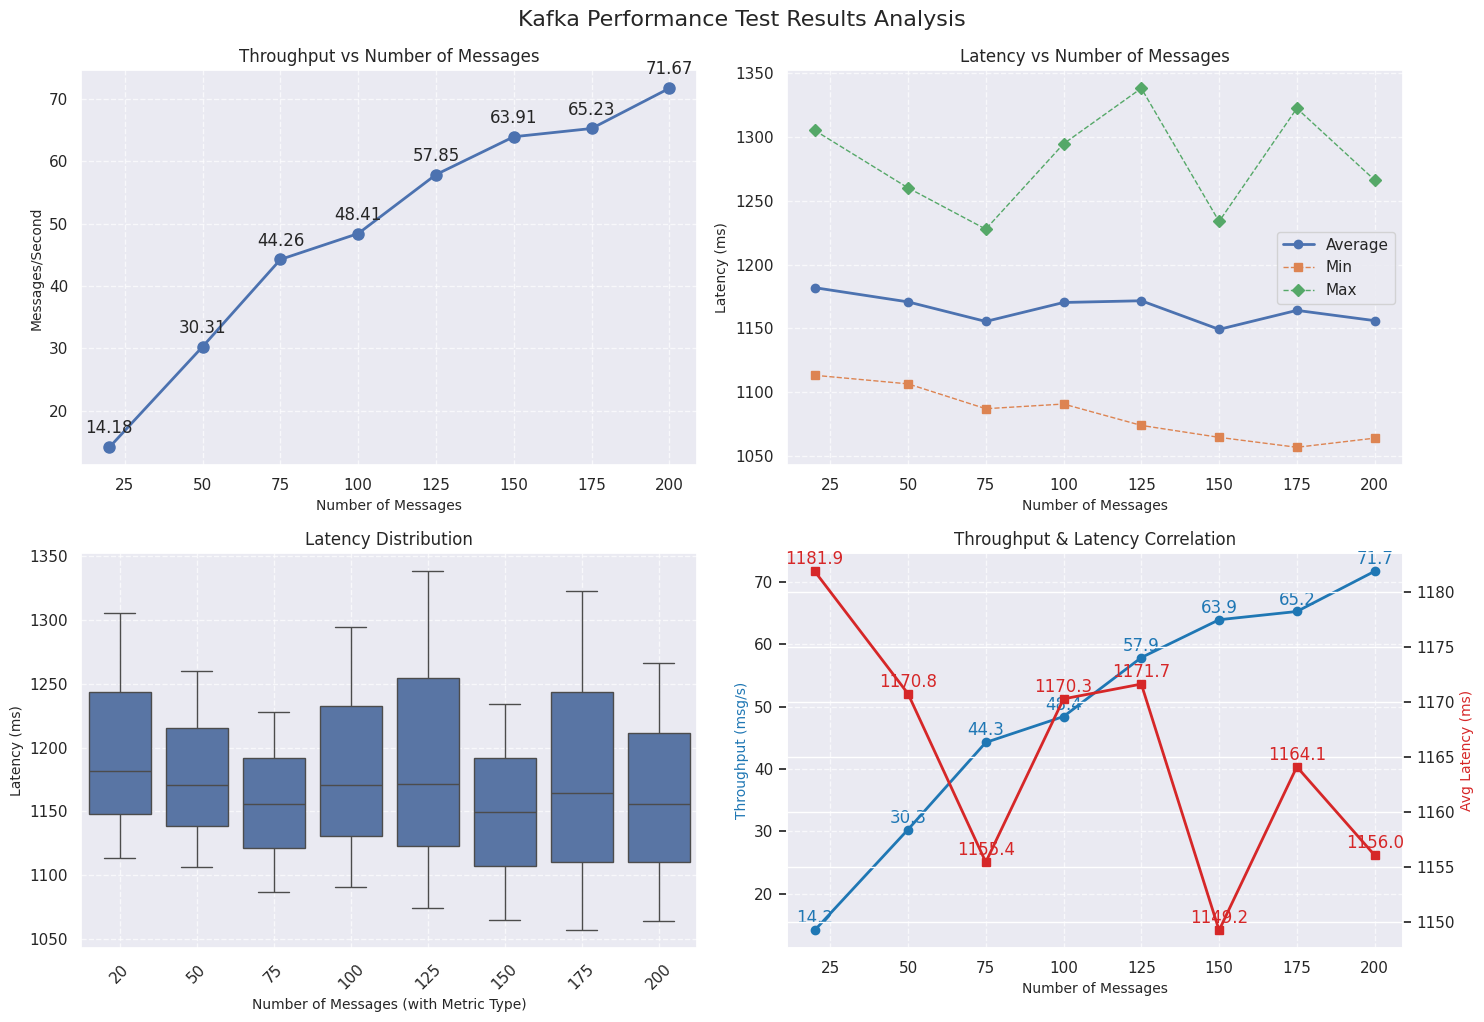
\includegraphics[width=\linewidth]{Images//C7/testchart.png}
    \vspace{10pt}
    \caption{Biểu đồ đánh giá hiệu năng Kafka trên Confluent Cloud}
    \label{fig:enter-label}
\end{figure}
\textbf{Nhận xét}:
\begin{itemize}[label=--]
    \item \textbf{Thông lượng và số lượng tin nhắn}: thông lượng tăng ổn định theo số lượng messages gửi vào, từ 14.18 msg/s (25 messages) lên đến 71.67 msg/s (200 messages). Biểu đồ thể hiện hiệu suất hệ thống được mở rộng tốt với tải tăng dần, phản ánh khả năng scalability (mở rộng) của Kafka và Confluent Cloud. Tuy nhiên, tốc độ tăng throughput chậm lại sau mốc 125 messages, cho thấy điểm tiệm cận của hiệu suất hoặc giới hạn băng thông/partition.
    \item \textbf{Độ trễ và số lượng tin nhắn}: Độ trễ trung bình duy trì ổn định trong khoảng 1150–1200 ms, ngay cả khi số lượng messages tăng lên. Độ trễ nhỏ nhất giảm dần từ ~1125 ms xuống còn khoảng 1080 ms, cho thấy hiệu quả xử lý được cải thiện với khối lượng tải cao hơn. Độ trễ lớn nhất dao động mạnh (từ 1250 ms đến hơn 1300 ms), phản ánh rằng vẫn tồn tại những đỉnh tải (latency spike) có thể ảnh hưởng đến trải nghiệm thời gian thực nếu không được tối ưu.
    \item \textbf{Phân phối độ trễ}: Phân phối độ trễ tương đối đều trong từng mức tải, với độ lệch chuẩn vừa phải. Một số mức tải (125, 175) có dải phân bố latency rộng hơn, chứng tỏ có dao động nhất định trong hiệu suất khi hệ thống xử lý khối lượng dữ liệu lớn hơn. Không có trường hợp cực đoan (outlier nghiêm trọng), thể hiện hệ thống tương đối ổn định và đáng tin cậy.
    \item \textbf{Mối tương quan giữa Thông lượng và Độ trễ}: Biểu đồ này cho thấy khi throughput tăng, độ trễ trung bình không tăng theo, ngược lại còn giảm nhẹ từ ~1181 ms xuống ~1156 ms. Điều này phản ánh rằng Kafka hoạt động hiệu quả hơn dưới tải cao, nhờ vào cơ chế batch và xử lý bất đồng bộ của nó. Không có dấu hiệu nghẽn cổ chai khi throughput tăng — một kết quả rất tích cực cho việc mở rộng hệ thống theo chiều ngang.
\end{itemize}
=> \textbf{Kết luận}: Kết quả này xác nhận Kafka trên Confluent Cloud là giải pháp phù hợp cho các hệ thống cần xử lý luồng dữ liệu ổn định ở quy mô vừa, với tiềm năng mở rộng tuyến tính khi tăng số partitions. Độ trễ ổn định và không có outlier cực đoan là điểm mạnh nổi bật, đảm bảo độ tin cậy cho các ứng dụng nghiệp vụ quan trọng.
\subsection{Đánh giá hiệu năng thu thập dữ liệu phần cứng và phần mềm}
\noindent Nhóm đã tiến hành phát triển công cụ Collector để thu thập dữ liệu phần cứng và phần mềm. Collector được thiết kế như là một producer của Kafka. Collector được xây dựng dựa trên ngôn ngữ Python.\\ \\
Nhóm sẽ đánh giá Collector qua các tiêu chí như sau : Hiệu năng, độ chính xác và toàn vẹn dữ liệu, mức độ thân thiện.
\begin{enumerate}
    \item \textbf{Hiệu năng}\\
    Nhóm đã tiến hành chạy Collector với kết quả như sau:
    \begin{itemize}[label=--]
        \item Thời gian thực thi:
        Nhóm sử dụng thư viện Time của Python để tiến hành đánh giá qua 10 lần chạy thử và kết quả đạt được như sau :
        \begin{itemize}[label=\textbullet]
            \item Thời gian thực thi nhanh nhất: 3.2 s
            \item Thời gian thực thi chậm nhất: 3.6075 s
            \item Thời gian thực thi trung bình: 3.41 s
        \end{itemize}
        => Điều này cho thấy thời gian thực thi của công cụ khá ổn định, không có sự dao động lớn giữa các lần chạy. Các yếu tố ảnh hưởng nhỏ như tải của hệ thống hoặc môi trường thực thi có thể là nguyên nhân chính cho sự dao động này. Thời gian quét này khá phù hợp để tích hợp trong hệ thống IT asset management mà không gây gián đoạn hoạt động.

        \item Sử dụng tài nguyên hệ thống:\\
        Nhóm tiến hành đo dựa trên mức sử dụng CPU và RAM của tiến trình thực thi quét. Kết quả sau 10 lần chạy cho thấy:
        \begin{itemize}[label=\textbullet]
            \item RAM dao động từ 33MB đến 34MB là rất nhỏ và cho thấy công cụ Scanner sử dụng tài nguyên bộ nhớ một cách hiệu quả. Biên độ dao động 1MB cho thấy sự ổn định trong việc quản lý bộ nhớ, không có dấu hiệu rò rỉ bộ nhớ (memory leak).
            \item CPU dao động từ 0.00\% đến 0.1\%. Điều này thể hiện rằng công cụ Collector không chiếm dụng tài nguyên CPU đáng kể trong quá trình quét.
        \end{itemize}
    \end{itemize}
    \item \textbf{Mức độ thân thiện}
    \begin{itemize}[label=--]
        \item Collector được thiết kế để chạy ngầm trên máy mà không ảnh hưởng đến nhân viên khi sử dụng máy tính để bàn và laptop cá nhân.  
        \item Nhân viên IT có thể dễ dàng cài đặt công cụ Collector trên tài sản máy tính mới.
        \item Tuy nhiên, Collector mới chỉ có khả năng cài đặt trên môi trường Window với phiên bản tối thiểu là Windows 7.
        \item Quy trình chạy Collector đơn giản, nhân viên IT chỉ cần bấm nút chạy và cài đặt cho chương trình khởi động cùng máy là có thể vận hành.
    \end{itemize}
    => Collector được thiết kế thân thiện với người dùng nhưng chưa có khả năng tương thích với đa nền tảng. 
    \\ Quy trình vận hành đơn giản nhằm đơn giản hóa các quy trình cho hệ thống. 
    \item \textbf{Toàn vẹn dữ liệu}\\
     Các trường hợp ảnh hưởng đến khả năng toàn vẹn dữ liệu:
        \begin{itemize}[label=--]
            \item Server Kafka sập: thông tin từ Collector sẽ không đến được Kafka Server.
            \item Lỗi hệ thống: hệ điều hành quá cũ hoặc không tương thích với hệ điều hành sẽ khiến cho dữ liệu bị thiếu mất hoặc không thu thập được
            \item Tắc nghẽn mạng: tình trạng mạng tắc nghẽn sẽ làm gói tin mà Producer gửi đến Kafka Server chậm, làm mất đi độ chính xác về thời gian.
        \end{itemize}
\end{enumerate}

\subsection{Đánh giá hiệu suất hệ thống}
\subsubsection{Giới thiệu công cụ và chỉ số đánh giá}
\noindent Để đánh giá hiệu năng hệ thống, nhóm sử dụng công cụ mã nguồn mở \textbf{K6} \cite{k6} – một nền tảng kiểm thử hiệu suất hiện đại được thiết kế để kiểm tra khả năng chịu tải của hệ thống backend. K6 hỗ trợ viết kịch bản bằng JavaScript, có thể mô phỏng hàng nghìn người dùng ảo (VUs – Virtual Users) thực hiện các hành động giống người dùng thật.
\begin{figure}[H]
    \centering
    
\includegraphics[width=0.5\linewidth]{Images/C7/k6.png}
    \vspace{15pt}
    \caption{K6\\ Nguồn: k6.io, truy cập vào ngày 01/05/2025}
\end{figure}
\noindent Các chỉ số quan trọng được đo trong quá trình đánh giá:
\begin{itemize}[label=--]
    \item \textbf{HTTP request duration (http\_req\_duration)}: Thời gian từ khi gửi request đến khi nhận toàn bộ phản hồi từ máy chủ.
    \item \textbf{Response time percentiles (p90, p95)}: Phân vị thống kê thời gian phản hồi – ví dụ, \textit{p90} nghĩa là 90\% request có thời gian phản hồi thấp hơn giá trị này.
    \item \textbf{Checks}: Tỉ lệ các điều kiện được kiểm tra (ví dụ mã phản hồi 200 hoặc thời gian phản hồi < 2000ms) đạt yêu cầu.
    \item \textbf{Http request failed (http\_req\_failed)}: Tỉ lệ request bị lỗi (timeout, lỗi mạng, hoặc lỗi server).
    \item \textbf{VUs và VUs max}: Số người dùng ảo đồng thời đang chạy và giá trị cực đại theo cấu hình.
\end{itemize}
\noindent Các chỉ số này giúp đánh giá toàn diện khả năng phản hồi và mức độ ổn định của hệ thống trong điều kiện tải thực tế và cực đại.

\subsubsection{Đánh giá hiệu suất}
\noindent Để kiểm tra khả năng chịu tải và hiệu suất phản hồi của hệ thống quản lý tài sản CNTT (ITAM), nhóm đã tiến hành kiểm thử hiệu năng sử dụng K6. Kịch bản kiểm thử được thiết kế mô phỏng 200 người dùng ảo (Virtual Users - VUs) truy cập đồng thời vào các API cốt lõi trong vòng 60 giây, lặp lại nhiều lần để thu thập dữ liệu ổn định.
\subsubsection*{1. Danh mục API đánh giá}
\begin{table}[H]
    \centering
    \caption{Các API cần test hiệu suất theo mục tiêu}
    \begin{tabular}{|>{\raggedright\arraybackslash}p{6cm}|>{\raggedright\arraybackslash}p{8cm}|}
        \hline
        \textbf{Mục tiêu chính} & \textbf{API liên quan nên test hiệu suất} \\
        \hline
        Dashboard \& Tổng quan (thường tải mỗi lần đăng nhập) & 
        \texttt{GET /api/dashboard}\newline
        \texttt{GET /api/overview/computer}\newline
        \texttt{GET /api/overview/software}\newline
        \texttt{GET /api/overview/hardware} \\
        \hline
        Tải danh sách tài sản (asset) & 
        \texttt{GET /api/asset}\newline
        \texttt{GET /api/computer/GetComputers}\newline
        \texttt{GET /api/Software} \\
        \hline
        Giám sát hiệu suất \& cảnh báo & 
        \texttt{GET /api/performance/\{assetId\}/\{topic\}}\newline
        \texttt{GET /api/alert}\newline
        \texttt{GET /api/alert/computer/\{computerId\}} \\
        \hline
        Thêm mới / cập nhật asset hoặc alert & 
        \texttt{POST /api/asset}\newline
        \texttt{POST /api/alert}\newline
        \texttt{PUT /api/computer/UpdateComputer/\{id\}} \\
        \hline
        Đăng nhập / xác thực & 
        \texttt{POST /api/login}\newline
        \texttt{GET /api/current-user}\newline
        \texttt{POST /api/refresh-token} \\
        \hline
        Kafka / gửi dữ liệu từ agent & 
        \texttt{POST /api/kafka/firstScan}\newline
        \texttt{POST /api/kafka/upgrade} \\
        \hline
        Dự đoán hiệu suất & 
        \texttt{GET /api/performance/predict}\newline
        \texttt{POST /api/performance/predict/test} \\
        \hline
    \end{tabular}
    
\end{table}

\subsubsection*{2. Tiêu chuẩn đánh giá}
\begin{itemize}[label=--]
\item Mã trạng thái HTTP: \textbf{200} (thành công)
\item Thời gian phản hồi: \textbf{< 2000ms}
\item Không có lỗi kết nối hoặc xử lý TLS
\end{itemize}

\subsubsection*{3. Chi tiết kết quả theo nhóm API}
\begin{table}[H]
\centering
\caption{Kết quả đánh giá hiệu năng Dashboard API}
\begin{tabular}{|>{\raggedright\arraybackslash}p{4cm}|l|>{\raggedright\arraybackslash}p{7cm}|}
\hline
\multicolumn{1}{|c|}{\textbf{Chỉ số đánh giá}} & \textbf{Giá trị} & \multicolumn{1}{c|}{\textbf{Phân tích}} \\
\hline
\textbf{Tỷ lệ thành công HTTP 200} & 100\% (22800/22800) & Tất cả các yêu cầu đều được xử lý thành công, không có lỗi phản hồi từ máy chủ \\
\hline
\textbf{Thời gian phản hồi trung bình} & 61.76ms & Hệ thống phản hồi rất nhanh, chỉ mất khoảng 62ms để xử lý mỗi request — nhanh hơn nhiều so với ngưỡng tiêu chuẩn 2000ms \\
\hline
\textbf{Phân vị 90 (P90)} & 87.19ms & 90\% số request có thời gian phản hồi dưới 87.19ms, cho thấy sự ổn định rất cao về hiệu suất \\
\hline
\textbf{Phân vị 95 (P95)} & 461.91ms & 95\% request phản hồi dưới 500ms, một tỷ lệ chấp nhận được trong môi trường sản phẩm thực tế \\
\hline
\textbf{Thời gian phản hồi nhanh nhất} & 0.31ms & Phản hồi cực nhanh ở điều kiện lý tưởng, cho thấy không có độ trễ từ phía máy chủ \\
\hline
\textbf{Thời gian phản hồi chậm nhất} & 1.77s & Dù một số trường hợp phản hồi chậm, nhưng vẫn trong mức cho phép (<2s), không ảnh hưởng nhiều đến trải nghiệm người dùng \\
\hline
\textbf{Tỷ lệ lỗi} & 0\% & Không có lỗi phát sinh trong toàn bộ quá trình kiểm thử, cho thấy độ ổn định cao \\
\hline
\textbf{Lưu lượng request} & 186.68 req/s & Hệ thống xử lý trung bình gần 187 request mỗi giây, duy trì được hiệu năng ổn định dưới tải \\
\hline
\textbf{User ảo (VUs)} & 21--200 & Số lượng người dùng mô phỏng thay đổi theo kịch bản kiểm thử, giúp đánh giá khả năng mở rộng của hệ thống \\
\hline
\end{tabular}

\end{table}

\begin{table}[H]
\centering
\caption{Kết quả đánh giá hiệu năng Asset API}
\begin{tabular}{|>{\raggedright\arraybackslash}p{4cm}|l|>{\raggedright\arraybackslash}p{7cm}|}
\hline
\textbf{Chỉ số đánh giá} & \textbf{Giá trị} & \textbf{Phân tích} \\
\hline
\textbf{Tỷ lệ thành công HTTP 200} & 100\% (22800/22800) & Tất cả các request đến các API chính đều được xử lý thành công, không có lỗi xảy ra \\
\hline
\textbf{Thời gian phản hồi trung bình} & 78.38ms & Phản hồi trung bình rất tốt, thấp hơn nhiều so với ngưỡng khuyến nghị 2000ms \\
\hline
\textbf{Phân vị 90 (P90)} & 218.72ms & 90\% request có phản hồi dưới 219ms, hiệu suất ổn định và đáng tin cậy \\
\hline
\textbf{Phân vị 95 (P95)} & 514.24ms & 95\% request phản hồi dưới 515ms, phù hợp cho môi trường thực tế \\
\hline
\textbf{Phản hồi nhanh nhất} & 0ms & Một số request được phản hồi gần như tức thì, không có độ trễ đáng kể \\
\hline
\textbf{Phản hồi chậm nhất} & 666.43ms & Request chậm nhất vẫn dưới 1s, đảm bảo không gây ảnh hưởng lớn đến trải nghiệm người dùng \\
\hline
\textbf{Tỷ lệ lỗi} & 0\% & Không có lỗi hệ thống nào phát sinh trong toàn bộ quá trình\\
\hline
\textbf{Lưu lượng request} & (181.87 req/s) & Hệ thống xử lý gần 182 yêu cầu mỗi giây, hiệu năng cao dưới tải vừa phải \\
\hline
\textbf{User ảo (VUs)} & 40--200 & Số lượng user mô phỏng tăng dần để kiểm tra khả năng chịu tải theo thời gian \\
\hline
\end{tabular}
\end{table}

\subsubsection*{Nhận xét tổng quan:}
\begin{itemize}[label=--]
\item Tất cả các API được đánh giá đều hoạt động ổn định với:
\begin{itemize}[label=\textbullet]
\item \textbf{Tỷ lệ thành công 100\%}, không có lỗi hệ thống trong suốt quá trình kiểm thử (tổng cộng 22,800 request)
\item \textbf{Thời gian phản hồi trung bình thấp}, dao động trong khoảng 62ms đến 78ms — thấp hơn rất nhiều so với ngưỡng tiêu chuẩn 2000ms
\item \textbf{Phân vị P90 và P95} đều nằm trong khoảng dưới 220ms và 515ms, phản ánh hiệu suất nhất quán và độ trễ thấp
\item \textbf{Lưu lượng xử lý cao} với trung bình khoảng 182 request mỗi giây, cho thấy hệ thống đủ khả năng phục vụ đồng thời nhiều người dùng
\item \textbf{Không có request thất bại}, chứng minh tính ổn định và đáng tin cậy của hệ thống trong điều kiện tải trung bình đến cao
\end{itemize}
\item Với kết quả này, hệ thống có thể hoạt động với hiệu năng ổn định ở tải vừa, sẵn sàng đưa vào vận hành thực tế. Tuy nhiên với dữ liệu lớn hơn cần kiểm thử và tối ưu thêm về mặt hiệu năng.
\end{itemize}

\subsubsection{Yêu cầu chức năng}
\begin{table}[H]
    \centering
    \caption{Checklist đánh giá yêu cầu chức năng}
    \begin{tabular}{|l|l|l|}
        \hline
        \textbf{Yêu cầu chức năng} & \textbf{Nhóm người dùng} & \textbf{Yes/No} \\
        \hline
        Giám sát tài sản & Nhân viên IT & Yes \\
        \hline
        Quản lý vòng đời tài sản & Quản lý, Nhân viên IT & Yes \\
        \hline
        Quản lý dữ liệu phần cứng và phần mềm & Nhân viên IT & Yes \\
        \hline
        Quản lý tài chính & Quản lý & Yes \\
        \hline
        Quản lý đơn đặt hàng & Quản lý & Yes \\
        \hline
        Cảnh báo và thông báo & Nhân viên IT & Yes \\
        \hline
        Tích hợp với các hệ thống khác & Quản trị viên hệ thống & No \\
        \hline
        Theo dõi hợp đồng bảo trì & Quản lý, Nhân viên IT & Yes \\
        \hline
        Quản lý giấy phép phần mềm & Quản lý, Nhân viên IT & Yes \\
        \hline
        Quản lý tuân thủ quy định & Quản lý & No \\
        \hline
        Báo cáo và phân tích & Quản lý & Yes \\
        \hline
        Quản lý sự cố và bảo trì tài sản & Nhân viên IT & Yes \\
        \hline
        Theo dõi thông tin địa điểm tài sản & Nhân viên IT & Yes \\
        \hline
        Dự báo hiệu suất hoạt động của tài sản & Nhân viên IT & Yes \\
        \hline
        Phân quyền người dùng & Quản trị viên hệ thống & Yes \\
        \hline
        Kiểm soát truy cập và đăng nhập an toàn & Quản trị viên hệ thống & Yes \\
        \hline
        Quản lý cài đặt và cấu hình hệ thống & Quản trị viên hệ thống & Yes \\
        \hline
    \end{tabular}
    
\end{table}
\subsubsection{Yêu cầu phi chức năng}
\begin{table}[H]
\centering
\caption{Checklist đánh giá yêu cầu phi chức năng}
\begin{tabular}{|p{3cm}|p{5cm}|p{1.3cm}|p{5cm}|}
\hline
\textbf{Yêu cầu} & \textbf{Thước đo} & \textbf{Yes/No} & \textbf{Ghi chú} \\
\hline
Hiệu suất & Thời gian phản hồi dưới 3s cho các yêu cầu từ người dùng & Yes & Đảm bảo phản hồi nhanh (trung bình dưới 100ms), vượt xa yêu cầu \\
\cline{2-4}
& Hỗ trợ ít nhất 500 yêu cầu đồng thời mà không giảm hiệu suất & Yes & Hệ thống xử lý 182 RPS trong điều kiện kiểm thử, có thể nâng cao với tuning nhẹ \\
\hline
Khả năng mở rộng & Hỗ trợ quản lý từ 500 đến 100,000 tài sản & Yes & Hiệu năng ổn định ở tải vừa, cần kiểm thử thêm với dữ liệu lớn để xác minh toàn diện \\
\hline
Bảo mật & Hỗ trợ xác thực đa yếu tố (MFA), mã hóa dữ liệu nhạy cảm & No & Hiện tại chỉ sử dụng xác thực qua JWT token; chưa triển khai cơ chế xác thực đa yếu tố (VD: OTP, xác minh email, app bảo mật) \\
\cline{2-4}
& Kiểm soát truy cập theo vai trò (RBAC) & Yes & Đã triển khai phân quyền chi tiết theo vai trò người dùng (Admin, ITStaff, Manager) \\
\hline
\multirow{2}{3cm}{Tính sẵn sàng và độ tin cậy} 
& Đảm bảo thời gian hoạt động 99.9\%, tối đa 1 giờ ngừng mỗi tháng & Yes & \multirow{2}{5cm}{Đã triển khai cơ chế backup và recovery cơ bản, cần kiểm thử thêm để đánh giá hiệu quả thực tế} \\
\cline{2-3}
& Phục hồi trong vòng 1 giờ sau sự cố & Yes & \\
\hline
Tính dễ sử dụng & Giao diện thân thiện, thao tác chính thực hiện trong số bước hợp lý (5–8 bước với các tác vụ tùy biến) & Yes & Giao diện hỗ trợ thao tác theo luồng rõ ràng, phù hợp với tính chất tùy biến cao của hệ thống \\
\hline
Tuân thủ & Hỗ trợ quy định GDPR, SOX & Yes & Có log đầy đủ hoạt động người dùng \\
\hline
Hỗ trợ \& bảo trì & Hỗ trợ khách hàng 24/7, cập nhật thường xuyên & No & Hiện tại chưa hỗ trợ đầy đủ 24/7, cần bổ sung quy trình cập nhật định kỳ \\
\hline
\end{tabular}

\end{table}


\subsection{Kết chương}
\noindent Nhóm đã thực hiện đánh hiệu năng thu thập dữ liệu thời gian thực với Kafka truyền thống cũng như Kafka Confluent Cloud, đánh giá hiệu năng cho thu thập dữ liệu phần cứng và phần mềm và đánh giá các yêu cầu chức năng lẫn phi chức năng.
\begin{itemize}[label=--]
    \item Với \textbf{Kafka truyền thống} nhóm đã chia 2 phần đánh giá là đánh giá Producer và đánh giá Consumer. 
    \begin{itemize}[label=\textbullet]
        \item Về Producer: Kafka cho thấy khả năng mạnh mẽ của mình khi được sử dụng trong môi trường thời gian thực qua khả năng xử lý lượng lớn dữ liệu được tạo ra. Tuy vẫn có độ trễ nhất định nhưng con số này khá nhỏ và ít ảnh hưởng đến ràng buộc thời gian thực mà hệ thống phải đáp ứng
        \item Về Consumer: Kafka Consumer có hiệu năng ổn đinh với tốc độ tiêu thụ dữ liệu ổn định và độ trễ thấp. Tuy nhiên vẫn cần rebalance, mặt khác rebalance này tương đối nhỏ không ảnh hưởng nhiều đến hệ thống.
    \end{itemize}
    \item Với \textbf{Kafka Confluent Cloud} nhóm đã triển khai đánh giá dựa trên mức tải và độ trễ. Từ kết quả có thể thấy được, sử dụng Kafka trên Confluent Cloud là giải pháp gọn, nhẹ hơn nhưng vẫn đảm bảo được hiệu suất hơn nữa việc triển khai với Cloud giúp việc mở rộng của hệ thống trở nên dễ dàng hơn.
    \item Với \textbf{công cụ thu thập dữ liệu phần cứng và phần mềm} nhóm đã thực hiện đánh giá hiệu năng, mức độ thân thiện và độ chính xác, toàn vẹn của dữ liệu.
    \begin{itemize}[label=\textbullet]
        \item Về hiệu năng: công cụ tương đối nhẹ, ít tốn tài nguyên của máy tính thích hợp để cài đặt các máy có cấu hình thấp.
        \item Về mức độ thân thiện: cách cài đặt và vận hành tương đối đơn giản nhưng cần cải thiện về khả năng đa hệ điều hành.
        \item Về độ chính xác và toàn vẹn dữ liệu: công cụ đảm bảo tương đối độ chính xác và toàn vẹn dữ liệu. Tuy nhiên vẫn cần phải đưa ra những biện pháp xử lý khi các điều kiện xấu từ bên ngoài tác động vào như môi trường mạng, cấu hình thiết bị, cấu hình hạ tầng máy chủ.
    \end{itemize}
    \item Với \textbf{hiệu suất hệ thống ITAM}, nhóm đã sử dụng Grafana K6 để đánh giá. Dựa trên kết quả đạt được cho thấy hệ thống có hiệu năng ổn định ở mức tải vừa và sẵn sàng để đưa vào thực tế. 
    \item \textbf{Với yêu cầu chức năng}: nhóm đã hoàn thiện gần như tất cả các yêu cầu đặt ra. Tuy nhiên vẫn chưa có hoàn thành hai yêu cầu đó là "Tích hợp với các hệ thống khác" và "Quản lý tuân thủ quy định"
    \item \textbf{Với yêu cầu phi chức năng}, nhóm cũng đã đạt được hầu như tất cả yêu cầu đặt ra nhưng vẫn còn một số hạn chế nhất định.
\end{itemize}


% \newpage
% \section{Triển khai hệ thống}
\subsection{Đóng gói với Docker}
\noindent Để đảm bảo khả năng triển khai đồng nhất và dễ dàng quản lý các dịch vụ trong dự án, toàn bộ hệ thống được đóng gói và triển khai thông qua \textbf{Docker}. Hệ thống bao gồm 4 thành phần chính: Frontend (Next.js), Backend (ASP.NET Core), Database (SQL Server), và AI Server (FastAPI - Python).

\begin{enumerate}
    \item \textbf{Sử dụng Dockerfile cho từng thành phần:}
    
    \textbf{Frontend (Next.js):}
    \begin{itemize}[label=--]
        \item Sử dụng multi-stage Dockerfile: giai đoạn đầu để build source bằng \texttt{npm run build}, giai đoạn hai để chạy ứng dụng bằng \texttt{npm run start}.
        \item Dùng image \texttt{node:18-alpine} để đảm bảo kích thước image nhỏ và hiệu năng cao.
    \end{itemize}
    
    \textbf{Backend (ASP.NET Core):}
    \begin{itemize}[label=--]
        \item Sử dụng multi-stage Dockerfile: giai đoạn đầu dùng \texttt{mcr.microsoft.com/dotnet/sdk:8.0} để build và publish; giai đoạn thứ hai dùng runtime \texttt{aspnet:8.0}.
        \item Tích hợp chứng chỉ số \texttt{.pfx} vào container để hỗ trợ HTTPS (port 443).
    \end{itemize}
    
    \textbf{AI Server (FastAPI - Python):}
    \begin{itemize}[label=--]
        \item Dùng image \texttt{python:3.12-slim}, tối ưu cài đặt bằng cách thêm tuỳ chọn \texttt{--no-cache-dir} khi cài dependencies.
        \item Chạy server bằng \texttt{uvicorn} tại cổng 8000.
    \end{itemize}
    
    \item \textbf{Quản lý container bằng Docker Compose:}
    
    Hệ thống được điều phối tập trung bằng một file \texttt{docker-compose.yml}, bao gồm 4 dịch vụ chính:

    \begin{itemize}[label=--]
        \item \textbf{sqlserver:} Dùng image SQL Server 2022, gắn volume \texttt{sqlserver-data} để lưu trữ dữ liệu bền vững. Cổng mặc định ánh xạ ra ngoài là 1434.
        
        \item \textbf{backend:} Build từ thư mục \texttt{./Backend}, cấu hình biến môi trường để:
        \begin{itemize}[label=\textbullet]
            \item Kết nối nội bộ với SQL Server qua Docker network.
            \item Sử dụng HTTPS với chứng chỉ số được mount vào container.
            \item Giao tiếp qua cổng 8080 (HTTP) và 443 (HTTPS).
        \end{itemize}
        
        \item \textbf{frontend:} Build từ thư mục \texttt{./Frontend}, chạy trên cổng 3000. Biến môi trường \texttt{NEXT\_PUBLIC\_BACKEND\_URL} được cấu hình để frontend có thể gọi API từ backend.
        
        \item \textbf{fastapi-predictor (AI Server):} Build từ thư mục chứa mã nguồn AI. Dịch vụ này:
        \begin{itemize}[label=\textbullet]
            \item Chạy trên cổng 8000 bằng \texttt{Uvicorn}.
            \item Mount thư mục \texttt{./model} vào container để sử dụng mô hình dự đoán.
            \item Cấu hình chính sách \texttt{restart: unless-stopped} để đảm bảo độ sẵn sàng.
        \end{itemize}
    \end{itemize}
\end{enumerate}

\subsection{Triển khai và cài đặt}
\noindent Hệ thống sử dụng trong nội bộ doanh nghiệp, vì thế sẽ được triển khai trong mạng nội bộ. Đầu tiên chúng ta cần đảm bảo có sẵn một máy chủ nội bộ (server) đã được cài đặt môi trường Docker và Docker Compose. Ngoài ra, cần kết nối internet để pull các image cần thiết.
\begin{enumerate}[leftmargin=*]
    \item \textbf{Khởi tạo cơ sở dữ liệu của hệ thống bằng cách chạy container SQL Server trước tiên:}
    
    Trước hết, cần chạy container SQL Server để khởi tạo cơ sở dữ liệu. Cơ sở dữ liệu sẽ được tự động tạo cùng với các bảng cần thiết dựa trên các tệp migration đã được chuẩn bị sẵn trong hệ thống.

    \item \textbf{Chạy container backend:}

    Sau khi cơ sở dữ liệu đã được khởi tạo thành công, tiếp theo là chạy container chứa ứng dụng backend. Ứng dụng backend sẽ đảm nhận vai trò cung cấp API và kết nối trực tiếp đến cơ sở dữ liệu để xử lý các yêu cầu từ người dùng và các dịch vụ khác.

    \item \textbf{Chạy container AI server và frontend:}

    Sau khi backend đã được triển khai ổn định, tiếp tục chạy các container cho AI server và frontend. 
    \begin{itemize}[label=--]
        \item \textbf{AI server} xử lý các tác vụ liên quan đến phân tích, dự đoán hoặc tự động hoá dựa trên dữ liệu thu thập được.
        \item \textbf{Frontend} là giao diện người dùng, cho phép quản trị viên hoặc nhân viên truy cập vào hệ thống, theo dõi trạng thái, xem báo cáo và thao tác với dữ liệu.
    \end{itemize}

    \item \textbf{Cài đặt ứng dụng Collector trên tất cả các máy tính cần giám sát và quản lý:} (các bước thực hiện xem chi tiết ở phụ lục)

    Các Collector là các ứng dụng nhẹ được cài đặt trên tất cả các máy tính trong hệ thống nội bộ cần theo dõi. Các Collector này sẽ:
    \begin{itemize}[label=--]
        \item Thu thập thông tin phần cứng (CPU, RAM, ổ cứng, v.v.).
        \item Thu thập thông tin phần mềm đã được cài đặt.
        \item Theo dõi hiệu suất hệ thống (mức sử dụng CPU, RAM, dung lượng ổ đĩa...).
        \item Gửi dữ liệu theo thời gian thực hoặc định kỳ về server để lưu trữ và phân tích.
    \end{itemize}

    \item \textbf{Cấu hình hệ thống giám sát và cảnh báo:}

    Sau khi hệ thống đã hoạt động ổn định, cần thiết lập các quy tắc cảnh báo để phát hiện các bất thường, ví dụ:
    \begin{itemize}[label=--]
        \item Cảnh báo khi máy tính sử dụng quá 90\% CPU trong thời gian dài.
        \item Gửi email hoặc thông báo cho quản trị viên khi có sự cố xảy ra.
    \end{itemize}

    \item \textbf{Kiểm tra và đánh giá hệ thống:}

    Sau khi triển khai xong, cần tiến hành kiểm tra toàn bộ các chức năng của hệ thống để đảm bảo hoạt động ổn định và đúng yêu cầu. Có thể thực hiện một số bài test như:
    \begin{itemize}[label=--]
        \item Kiểm tra dữ liệu từ Collector có được gửi đầy đủ và chính xác.
        \item Đảm bảo frontend hiển thị đúng thông tin và API phản hồi nhanh.
        \item Kiểm tra khả năng mở rộng và hiệu suất của hệ thống khi có nhiều máy kết nối đồng thời.
    \end{itemize}
\end{enumerate}

\subsection{Kết chương}
\noindent Trong chương này, nhóm đã trình bày chi tiết quá trình đóng gói và triển khai hệ thống giám sát, quản lý tài sản công nghệ thông tin nội bộ thông qua công nghệ Docker. Việc sử dụng Docker và Docker Compose không chỉ giúp chuẩn hóa môi trường triển khai, mà còn đảm bảo tính linh hoạt, dễ dàng mở rộng và bảo trì hệ thống. \\ \\
Thông qua việc cấu hình và vận hành các dịch vụ thành phần như Frontend, Backend, AI Server và Database, hệ thống có thể hoạt động ổn định trong môi trường mạng nội bộ doanh nghiệp. Bên cạnh đó, việc triển khai các Collector trên từng máy trạm và thiết lập cơ chế giám sát, cảnh báo theo thời gian thực đã góp phần nâng cao hiệu quả quản lý, kịp thời phát hiện các bất thường trong hệ thống. Sau cùng, cần phải có các bước kiểm tra đánh giá nhằm đảm bảo hệ thống sẵn sàng cho hoạt động thực tế.
% \newpage
% \section{Tổng kết}
\noindent \textit{Trong chương này, nhóm tác giả sẽ tổng kết quá trình thực hiện đề tài. Từ đó, đánh giá được đóng góp của hệ thống, kết quả đạt được và hạn chế tồn tại, cũng như xây dựng được hướng phát triển cho hệ thống.}
\subsection{Kết quả đạt được}
\noindent Trong quá trình thực hiện đồ án, nhóm đã đạt được những kết quả bao gồm:
\begin{itemize}[label=--]
    \item Tìm hiểu về các kiến thức liên quan đến lĩnh vực giám sát và quản lý tài sản công nghệ thông tin.
    \item Xây dựng hệ thống giám sát tài sản IT theo thời gian thực và hỗ trợ các tính năng quản lý tài sản: Hệ thống cung cấp khả năng theo dõi hoạt động của các máy tính và tài sản IT trong mạng doanh nghiệp một cách liên tục và chính xác, cũng như khả năng quản lý tài sản IT của doanh nghiệp.
    \item Tích hợp công nghệ thu thập dữ liệu real-time cụ thể là Apache Kafka truyền thống và Kafka trên Confluent Cloud vào dự án.
    \item Phát triển tính năng cảnh báo sớm với mô hình dự đoán hiệu suất tài sản sử dụng mạng LSTM.
    \item Thực hiện kiểm thử, đánh giá hệ thống để kiểm tra khả năng triển khai trong thực tế.
    \item Tìm hiểu và thực hiện đóng gói và triển khai hệ thống trong nội bộ công ty, tổ chức.
\end{itemize}
\subsection{Những đóng góp của hệ thống}

\noindent Trong quá trình thực hiện đồ án, hệ thống quản lý tài sản CNTT thời gian thực đã mang lại một số đóng góp quan trọng cả về mặt học thuật lẫn thực tiễn, cụ thể như sau:

\begin{itemize}[label=--]
    \item \textbf{Đóng góp về kiến thức:} Nhóm đã nghiên cứu và hệ thống hóa các kiến thức liên quan đến lĩnh vực giám sát và quản lý tài sản công nghệ thông tin, bao gồm các nguyên lý giám sát tài sản, quản lý vòng đời, đánh giá hiệu năng và ứng dụng công nghệ thời gian thực.
    
    \item \textbf{Xây dựng hệ thống giám sát tài sản IT theo thời gian thực:} Hệ thống cho phép theo dõi hoạt động của các thiết bị IT trong doanh nghiệp một cách liên tục và chính xác. Qua đó hỗ trợ công tác quản lý tài sản hiệu quả hơn, giảm thiểu rủi ro từ việc thiếu thông tin hoặc quản lý rời rạc.

    \item \textbf{Tích hợp công nghệ thu thập dữ liệu real-time:} Hệ thống ứng dụng Apache Kafka truyền thống và Kafka trên nền tảng Confluent Cloud để thu thập dữ liệu hiệu suất từ các máy tính trong mạng nội bộ theo thời gian thực, đảm bảo tính mở rộng, ổn định và khả năng xử lý dữ liệu lớn. Với Kafka Confluent Cloud, hệ thống giờ đây có khả năng thu thập dữ liệu từ xa, bất kể vị trí địa lý, chỉ cần thiết bị có kết nối với Internet thì sẽ được quản lý và giám sát.

    \item \textbf{Ứng dụng trí tuệ nhân tạo trong quản lý tài sản:} Việc phát triển mô hình LSTM nhằm dự đoán hiệu suất sử dụng CPU và RAM của các thiết bị giúp hệ thống đưa ra cảnh báo sớm về các nguy cơ quá tải hoặc suy giảm hiệu năng. Đây là bước tiến quan trọng trong việc áp dụng AI vào công tác vận hành hạ tầng IT.

    \item \textbf{Kiểm thử và đánh giá toàn diện:} Hệ thống được kiểm thử qua nhiều kịch bản khác nhau, kiểm tra khả năng xử lý dữ liệu, phản hồi API, tính chính xác của mô hình dự đoán và độ ổn định khi triển khai trong môi trường thực tế.

    \item \textbf{Khả năng triển khai thực tế:} Dự án không chỉ dừng lại ở mức mô phỏng mà còn được nhóm đóng gói và triển khai thử nghiệm nội bộ, đảm bảo khả năng áp dụng thực tế trong các doanh nghiệp, tổ chức có nhu cầu giám sát và quản lý tài sản IT.

\end{itemize}

\noindent Tóm lại, hệ thống là một giải pháp tiềm năng cho các doanh nghiệp trong việc hiện đại hóa công tác giám sát và quản lý tài sản CNTT, kết hợp hiệu quả giữa công nghệ thời gian thực và trí tuệ nhân tạo.

\subsection{Hạn chế và tồn tại của hệ thống}

\noindent Bên cạnh những kết quả đã đạt được, hệ thống vẫn còn tồn tại một số hạn chế nhất định, cụ thể như sau:

\begin{itemize}[label=--]
    \item \textbf{Chưa tối ưu hoá mô hình dự đoán:} Mô hình LSTM hiện tại được huấn luyện dựa trên tập dữ liệu tổng hợp chung cho tất cả các máy tính. Điều này có thể ảnh hưởng đến độ chính xác khi áp dụng cho từng thiết bị cụ thể với đặc điểm sử dụng khác nhau. Ngoài ra, việc tối ưu hyperparameter chưa được thực hiện đầy đủ do hạn chế thời gian. Ngoài ra do việc thu thập dữ liệu hiệu suất vẫn còn phức tạp nên dẫn đến chưa đủ dữ liệu.
    \item \textbf{Chưa hỗ trợ nhiều loại tài sản ngoài máy tính:} Phiên bản hiện tại của hệ thống chủ yếu áp dụng cho máy tính để bàn và laptop, chưa mở rộng đến các thiết bị khác như máy chủ, thiết bị mạng hoặc IoT. Ngoài ra công cụ thu thập dữ liệu hiện tại vẫn chỉ hỗ trợ cho hệ điều hành Window.
    \item \textbf{Thiếu các cơ chế bảo mật nâng cao:} Các cơ chế mã hóa dữ liệu truyền tải chưa được triển khai đầy đủ, gây hạn chế khi triển khai trong môi trường doanh nghiệp thực tế có yêu cầu bảo mật cao.
    \item \textbf{Hiệu năng hệ thống có thể bị ảnh hưởng khi mở rộng quy mô lớn:} Khi số lượng thiết bị gửi dữ liệu đồng thời tăng cao, cần đánh giá thêm khả năng chịu tải của hệ thống khi mở rộng quy mô trên 1000 máy, hiện chưa được thử nghiệm ở quy mô lớn.
\end{itemize}
\noindent Các vấn đề trên là những điểm mà nhóm sẽ tiếp tục cải thiện trong các giai đoạn phát triển tiếp theo nhằm hoàn thiện hệ thống và đáp ứng tốt hơn nhu cầu triển khai thực tế.

\subsection{Hướng phát triển trong tương lai}
\begin{itemize}[label=--]
\item \textbf{Tối ưu hoá mô hình dự đoán:} Trong giai đoạn tiếp theo, nhóm dự định huấn luyện mô hình LSTM riêng biệt cho từng nhóm thiết bị hoặc người dùng cụ thể để nâng cao độ chính xác. Đồng thời, sẽ thực hiện tối ưu các siêu tham số (hyperparameters) và mở rộng tập dữ liệu bằng cách cải tiến công cụ thu thập hiệu suất.
   \item \textbf{Mở rộng phạm vi thu thập dữ liệu:} Hệ thống hiện tại chỉ áp dụng cho máy tính để bàn và laptop sử dụng hệ điều hành Windows. Trong tương lai, nhóm sẽ mở rộng phạm vi hỗ trợ sang các nền tảng khác như Linux và macOS, cũng như các thiết bị như máy chủ, thiết bị mạng, IoT.

\item \textbf{Cải tiến hiệu năng và khả năng mở rộng:} Nhóm sẽ tiến hành thử nghiệm hệ thống ở quy mô lớn hơn (trên 1000 thiết bị), đồng thời cải thiện kiến trúc hạ tầng và tối ưu luồng xử lý Kafka để tăng khả năng chịu tải. Bên cạnh đó, hệ thống sẽ được nâng cấp để hỗ trợ quản lý và giám sát tài sản IT ở mọi vị trí địa lý—chỉ cần thiết bị có kết nối Internet, dữ liệu vẫn sẽ được thu thập và xử lý tập trung theo thời gian thực, đảm bảo khả năng giám sát từ xa toàn diện và không bị giới hạn bởi không gian địa lý.

\item \textbf{Tăng cường bảo mật:} Hệ thống sẽ được bổ sung các cơ chế bảo mật nâng cao như mã hóa dữ liệu đầu cuối (end-to-end encryption), xác thực đa yếu tố (MFA), kiểm soát truy cập chi tiết (RBAC) nhằm đáp ứng các yêu cầu khắt khe trong môi trường doanh nghiệp.

\item \textbf{Phát triển giao diện người dùng hiện đại và đa nền tảng:} Hướng tới việc nâng cấp UI/UX, nhóm sẽ thiết kế lại giao diện theo hướng hiện đại, thân thiện và có khả năng đáp ứng tốt trên các thiết bị di động và màn hình cảm ứng.

\item \textbf{Tích hợp phân tích dữ liệu nâng cao:} Bổ sung các module AI/ML để khai thác dữ liệu lịch sử và đưa ra dự đoán sâu hơn như tuổi thọ còn lại của thiết bị, khả năng hỏng hóc hoặc đề xuất thời điểm bảo trì tối ưu.

\item \textbf{Đa ngôn ngữ và khả năng triển khai quốc tế:} Nhóm sẽ triển khai hỗ trợ đa ngôn ngữ, đặc biệt là Tiếng Anh, nhằm phục vụ tốt hơn cho các tổ chức hoặc doanh nghiệp hoạt động trong môi trường quốc tế.

\item \textbf{Khảo sát người dùng và cải tiến dựa trên phản hồi thực tế:} Trong các giai đoạn tiếp theo, nhóm sẽ triển khai khảo sát người dùng trên diện rộng và tích hợp công cụ theo dõi hành vi người dùng nhằm thu thập dữ liệu về trải nghiệm thực tế, từ đó điều chỉnh và cải tiến hệ thống một cách hiệu quả và sát với nhu cầu sử dụng.

\end{itemize}



% \newpage
% \section*{Kế hoạch cho Đồ án Tốt nghiệp (Capstone Project)}
% \begin{figure}[H]
    \centering
    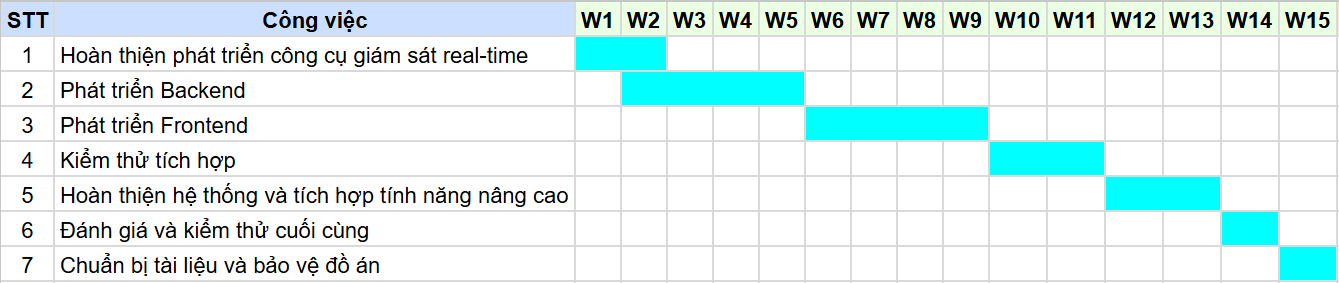
\includegraphics[width=16cm]{Images/GD2-Plan/datn-plan.png}
    \vspace{15pt}
    \caption{Kế hoạch tổng quan cho giai đoạn 2}
\end{figure}

\begin{itemize}

\item\textbf{Task 1: Hoàn thiện phát triển công cụ giám sát real-time (W1-2)}\\
\indent Mục tiêu:
\begin{itemize}
    \item Hoàn thành phát triển công cụ giám sát real-time cài trên máy tính
\end{itemize}
\begin{table}[H]
    \centering
    \begin{tabular}{|p{1cm}|p{8cm}|p{4cm}|}
        \hline
        \textbf{STT} & \textbf{Công việc cụ thể} & \textbf{Thành viên phụ trách} \\
        \hline
        1 & Xác định loại dữ liệu cần thu thập & Hiển   \\
        \hline
        2 & Xác định tần suất thu thập dữ liệu & Khang   \\
        \hline
        3 & Thiết kế công cụ giám sát & Khang  \\
        \hline
        4 & Phát triển công cụ giám sát bằng Python và Kafka & Khang   \\
        \hline
        5 & Kiểm tra lấy dữ liệu từ máy tính bằng công cụ giám sát & Khang, Hiển   \\
        \hline
    \end{tabular}
    
\end{table}

\item\textbf{Task 2: Phát triển Backend (W2-5)}\\
\indent Mục tiêu:
\begin{itemize}
    \item Xây dựng và triển khai các service và API theo thiết kế.
    \item Tích hợp API với cơ sở dữ liệu.
\end{itemize}
\begin{table}[H]
    \centering
    \begin{tabular}{|p{1cm}|p{8cm}|p{4cm}|}
        \hline
        \textbf{STT} & \textbf{Công việc cụ thể} & \textbf{Thành viên phụ trách} \\
        \hline
        1 & Xây dựng hạ tầng cơ bản và tích hợp cơ sở dữ liệu & Khang, Hiển \\
        \hline
        2 & Xây dựng microservice Asset Monitoring Service 
        \begin{itemize}
            \item Tích hợp Kafka Producer
            \item Triển khai Kafka Consumer
        \end{itemize} & Hiển \\
        \hline
        3 & Xây dựng microservice Alert \& Notification Service 
        \begin{itemize}
            \item Xây dựng chức năng và ngưỡng cảnh báo
            \item Tích hợp Kafka để nhận thông tin sự kiện cần gửi thông báo
            \item Tích hợp các phương thức gửi thông báo (email, SMS, push notification...)
            \item Lưu trữ thông tin vào database
        \end{itemize} & Khang\\
        \hline
        4 & Xây dựng User Management Service 
        \begin{itemize}
            \item Quản lý thông tin người dùng và phân quyền
            \item Sử dụng tiêu chuẩn bảo mật OAuth2 để xác thực và phân quyền
            \item Tích hợp JWT (JSON Web Token) hoặc Session-based Authentication
            \item Đảm bảo dữ liệu người dùng được mã hóa (hashed passwords)
        \end{itemize} & Hiển, Tiên \\
        \hline
        5 & Xây dựng Lifecycle Management Service 
        \begin{itemize}
            \item Quản lý vòng đời tài sản (máy tính, phần cứng, phần mềm)
        \end{itemize} & Khang, Hiển, Tiên \\
        \hline
        6 & Xây dựng Data Analysis \& Prediction Service 
        \begin{itemize}
            \item Xây dựng và huấn luyện model phân tích và gợi ý bảo trì tài sản
            \item Tích hợp với các service khác
        \end{itemize} & Khang \\
        \hline
        7 & Xây dựng Inventory Management Service 
        \begin{itemize}
            \item Quản lý thông tin tài sản (máy tính, phần cứng, phần mềm)
            \item Sử dụng UUID để quản lý tài sản
        \end{itemize} & Hiển, Tiên \\
        \hline
        8 & Xây dựng API Gateway 
        \begin{itemize}
            \item Tích hợp xác thực và bảo mật
            \item Rate-limiting, load balancing
        \end{itemize} & Hiển \\
        \hline
        9 & Viết Unit Test cho API & Tiên \\
        \hline
        10 & Kiểm thử các API bằng Postman hoặc Swagger để đảm bảo đúng logic & Tiên \\
        \hline
    \end{tabular}
\end{table}

\item\textbf{Task 3: Phát triển Frontend (W6-9)}\\
\indent Mục tiêu:
\begin{itemize}
    \item Hoàn thiện các màn hình chính đã thiết kế trong UI.
    \item Kết nối giao diện người dùng với API.
\end{itemize}
\begin{table}[H]
    \centering
    \begin{tabular}{|p{1cm}|p{8cm}|p{4cm}|}
        \hline
        \textbf{STT} & \textbf{Công việc cụ thể} & \textbf{Thành viên phụ trách} \\
        \hline
        1 & Tinh chỉnh giao diện Figma & Tiên \\
        \hline
        2 & Xây dựng các Reusable Components & Khang, Hiển, Tiên \\
        \hline
        3 & Sử dụng framework Angular để phát triển các giao diện chính cho các phần 
        \begin{itemize}
            \item Giám sát máy tính
            \item Quản lý máy tính
            \item Quản lý phần cứng
            \item Quản lý phần mềm
            \item Quản lý giấy phép
            \item Quản lý cảnh báo
            \item Quản lý yêu cầu nâng cấp
            \item Quản lý sự cố và bảo trì
            \item Quản lý đơn hàng
            \item Quản lý cấu hình cảnh báo
        \end{itemize} & Khang, Hiển, Tiên \\
        \hline
        4 & Xử lý tính năng giám sát thời gian thực, hiển thị dữ liệu thời gian thực trên giao diện &  Hiển, Tiên \\
        \hline
        5 & Xử lý luồng dữ liệu giữa frontend và backend & Khang \\
        \hline
        6 & Kiểm tra giao diện để đảm bảo hoạt động chính xác & Hiển\\
        \hline
    \end{tabular}
\end{table}

\item\textbf{Task 4: Kiểm thử tích hợp (W10-11)}\\
\indent Mục tiêu:
\begin{itemize}
    \item Đảm bảo hệ thống hoạt động đồng bộ giữa các thành phần (công cụ giám sát, frontend, backend, cơ sở dữ liệu).
\end{itemize}
\begin{table}[H]
    \centering
    \begin{tabular}{|p{1cm}|p{8cm}|p{4cm}|}
        \hline
        \textbf{STT} & \textbf{Công việc cụ thể} & \textbf{Thành viên phụ trách} \\
        \hline
        1 & 
        Chạy các kịch bản kiểm thử tích hợp:
        \begin{itemize}
            \item Tích hợp giữa các microservice
            \item Tích hợp giữa frontend và backend
            \item Tích hợp với cơ sở dữ liệu
        \end{itemize}
        Các loại kiểm thử:
        \begin{itemize}
            \item Kiểm thử chức năng
            \item Kiểm thử tích hợp
            \item Kiểm thử luồng nghiệp vụ (End-to-End Testing)
        \end{itemize} & Hiển, Tiên \\
        \hline
        2 & 
        Kiểm tra các trường hợp lỗi:
        \begin{itemize}
            \item Trường hợp lỗi hệ thống
            \item Trường hợp lỗi dữ liệu
            \item Trường hợp giao diện
        \end{itemize} & Khang \\
        \hline
        3 & 
        Xử lý lỗi phát sinh trong quá trình kiểm thử:
        \begin{itemize}
            \item Ghi nhận lỗi
            \item Phân loại lỗi
            \item Sửa lỗi
            \item Kiểm thử lại
        \end{itemize} & Khang, Hiển, Tiên \\
        \hline
    \end{tabular}
\end{table}

\item\textbf{Task 5: Hoàn thiện hệ thống và tích hợp tính năng nâng cao (W12-13)}\\
\indent Mục tiêu:
\begin{itemize}
    \item Cải tiến và tinh chỉnh giao diện, tính năng.
    \item Đảm bảo hiệu năng và độ ổn định của hệ thống.
    \item Thêm các tính năng nâng cao để cải thiện trải nghiệm người dùng.
\end{itemize}
\begin{table}[H]
    \centering
    \begin{tabular}{|p{1cm}|p{8cm}|p{4cm}|}
        \hline
        \textbf{STT} & \textbf{Công việc cụ thể} & \textbf{Thành viên phụ trách} \\
        \hline
        1 & 
        Chỉnh sửa, tối ưu giao diện người dùng để trực quan và thân thiện hơn. & Tiên \\
        \hline
        2 & 
        Kiểm tra và tối ưu hiệu suất API và cơ sở dữ liệu. & Khang, Hiển \\
        \hline
        3 & 
        Thực hiện và kiểm thử tính năng báo cáo tổng quan:
        \begin{itemize}
            \item Máy tính
            \item Phần cứng
            \item Phần mềm
        \end{itemize} & Khang, Hiển, Tiên \\
        \hline
    \end{tabular}
\end{table}

\item\textbf{Task 6: Đánh giá và kiểm thử cuối cùng (W14)}\\
\indent Mục tiêu:
\begin{itemize}
    \item Đảm bảo hệ thống sẵn sàng triển khai thực tế.
\end{itemize}
\begin{table}[H]
    \centering
    \begin{tabular}{|p{1cm}|p{8cm}|p{4cm}|}
        \hline
        \textbf{STT} & \textbf{Công việc cụ thể} & \textbf{Thành viên phụ trách} \\
        \hline
        1 & Kiểm tra toàn bộ hệ thống với các kịch bản thực tế. & Khang \\
        \hline
        2 & Chạy thử hệ thống trong môi trường doanh nghiệp thực tế và thu thập kết quả. & Hiển \\
        \hline
        3 & Sửa lỗi và cải tiến dựa trên kết quả chạy thử. &  Tiên \\
        \hline
    \end{tabular}
\end{table}

\item\textbf{Task 7: Chuẩn bị tài liệu và bảo vệ đồ án (W15)}\\
\indent Mục tiêu:
\begin{itemize}
    \item Hoàn thiện các tài liệu liên quan đến hệ thống.
    \item Chuẩn bị nội dung bảo vệ đồ án trước hội đồng.
\end{itemize}
\begin{table}[H]
    \centering
    \begin{tabular}{|p{1cm}|p{8cm}|p{4cm}|}
        \hline
        \textbf{STT} & \textbf{Công việc cụ thể} & \textbf{Thành viên phụ trách} \\
        \hline
        1 & Viết tài liệu hướng dẫn sử dụng hệ thống. & Khang, Hiển, Tiên \\
        \hline
        2 & Viết báo cáo đồ án. & Khang, Hiển, Tiên \\
        \hline
        3 & Chuẩn bị bài thuyết trình và luyện tập trả lời câu hỏi từ hội đồng. & Khang, Hiển, Tiên \\
        \hline
    \end{tabular}
\end{table}


\end{itemize}


\renewcommand\refname{}
\newpage
\section*{Tài liệu tham khảo}
\addcontentsline{toc}{section}{Tài liệu tham khảo}
\begin{thebibliography}{99999}
% \bibitem{thuctrang}
% % {Ứng dụng công nghệ thông tin trong quản lý, sử dụng tài sản công của ngành Tài chính.} \url{https://tapchinganhang.gov.vn/thuc-trang-va-giai-phap-phat-trien-cong-nghe-tai-chinh-tai-viet-nam.htm}
% \bibitem{kmc1}{IT Asset Management (ITAM)}, 15/09/2024, \url{https://invgate.com/guides/itam/}
% \bibitem{rtd}{Real-Time Data}, 26/09/2024 ,\url{https://en.wikipedia.org/wiki/Real-time_data}
% \bibitem{prtd}{Processing Real-time Data}, 27/09/2024 , \url{https://estuary.dev/what-is-real-time-processing/}
% \bibitem{trtd} {Type of Real-time Data}, 27/09/2024, \url{https://imply.io/blog/real-time-data-what-it-is-why-it-matters-and-more/}
% \bibitem{assetexplore}{AssetExplore. \emph{IT Asset Management Tool for your Business}, 19/09/2024, \url{https://www.manageengine.com/products/asset-explorer/}}
% \bibitem{reviewExplore}{ManageEngine AssetExplorer Review}, 19/09/2024 ,\url{https://www.forbes.com/advisor/business/software/manageengine-assetexplorer-review/}
% % \bibitem{snipeit}{Snipe IT. \url{https://snipeitapp.com/}}
% \bibitem{servicenow}{IT Asset Management (ITAM), ServiceNow, 20/09/2024, \url{https://www.servicenow.com/products/it-asset-management.html}}
% % \bibitem{nextjs}{Introduction, Nextjs. \url{https://nextjs.org/docs}}
% % \bibitem{python}{Python Introduction, W3Schools. \url{https://www.w3schools.com/python/python_intro.asp}}
% % \bibitem{typescript}{TypeScript Overview, TutorialsTeacher. \url{https://www.tutorialsteacher.com/typescript/typescript-overview#:~:text=TypeScript%20is%20an%20open%2Dsource,that%20compiles%20to%20plain%20JavaScript.}}
% % \bibitem{mui}{Material UI - Overview, MUI CORE. \url{https://mui.com/material-ui/getting-started/}}
% % \bibitem{servicedeskplus}{ManageEngine ServiceDesk Plus. \url{https://www.manageengine.com/products/service-desk/}}
% % \bibitem{maximo}{IBM Maximo Asset Management. \url{https://www.ibm.com/cloud/maximo-asset-management}}
% % \bibitem{webhelpdesk}{SolarWinds Web Help Desk. \url{https://www.solarwinds.com/web-help-desk}}
% % \bibitem{freshservice}{Freshservice - ITSM Software. \url{https://freshservice.com/}}
% % \bibitem{lansweeper}{Lansweeper - IT Asset Management. \url{https://www.lansweeper.com/}}
% % \bibitem{mui}{Material UI - Overview, MUI CORE. \url{https://mui.com/material-ui/getting-started/}}
% \bibitem{servicedeskplus}{ManageEngine ServiceDesk Plus, 20/09/2024, \url{https://www.manageengine.com/products/service-desk/}}
% \bibitem{invgate}{IT Asset Management Tool, InvGate Insight. 20/09/2024,\url{https://invgate.com/insight}}
% \bibitem{assetpanda}{Asset Panda, Asset Management \& Tracking Platform, 20/09/2024, 
% \url{https://www.assetpanda.com/our-technology/#all-features}}
% \bibitem{topitam}{Top 10 Best IT Asset Management Software, Jorge Farah, 21/09/2024
% \url{https://blog.invgate.com/best-it-asset-management-and-inventory-tools}}
% % \bibitem{maximo}{IBM Maximo Asset Management. \url{https://www.ibm.com/cloud/maximo-asset-management}}
% % \bibitem{webhelpdesk}{SolarWinds Web Help Desk. \url{https://www.solarwinds.com/web-help-desk}}
% % \bibitem{freshservice}{Freshservice - ITSM Software. \url{https://freshservice.com/}}
% % \bibitem{lansweeper}{Lansweeper - IT Asset Management. \url{https://www.lansweeper.com/}}
% \bibitem{accgroup}{Biên tập viên ACC, \emph{Tài sản công nghệ thông tin là gì?} Công ty Luật ACC, 10/09/2024, \url{https://accgroup.vn/tai-san-cong-nghe-thong-tin-la-gi}}
% % \bibitem{assetmanagement}{IT Asset Management, ServiceNow. \url{https://www.servicenow.com/products/it-asset-management.html}}

% \bibitem{kafka}{\emph{What is Apache Kafka?}, Confluent, 10/10/2024 \url{https://www.confluent.io/what-is-apache-kafka/}}

% \bibitem{plink}{\emph{What is Apache Flink?}, Confluent , 10/10/2024, \url{https://www.confluent.io/learn/apache-flink/}}

% \bibitem{}{\emph{Flink, Spark, Storm, Kafka: A Comparative Analysis of Big Data Stream Processing Frameworks for Your Business Project}, 10/10/2024 ,Roman Glushach \\\url{https://romanglushach.medium.com/flink-spark-storm-kafka-a-comparative-analysis-of-big-data-stream-processing-frameworks-for-dab3dd42fc16}}

% \bibitem{dotnet} \emph{Why Choose .NET: Pros and Cons of .NET Development}, Waverley Software, 25/10/2024, \url{https://waverleysoftware.com/blog/why-choose-net-pros-and-cons/}

% \bibitem{nodejs} \emph{When and Why to Use Node.js: An In-Depth Guide for 2024}, Relevant Software, \url{https://relevant.software/blog/why-and-when-to-use-node-js/}

% \bibitem{java} \emph{12 Pros and Cons of Java for Your Project}, Anywhere Club, \url{https://aw.club/global/en/blog/pros-and-cons-java}

% \bibitem{docker} \emph{Docker là gì?}, AWS, 10/10/2024 \url{https://aws.amazon.com/vi/docker/}

% \bibitem{kubernetes} \emph{Kubernetes là gì?}, Kubernetes.io, 10/10/2024\url{https://kubernetes.io/vi/docs/concepts/overview/what-is-kubernetes/}

% \bibitem{cicd} \emph{What is CI/CD?}, GitLab, 10/10/2024, \url{https://about.gitlab.com/topics/ci-cd/}

% \bibitem{websockets} \emph{The WebSocket API (WebSockets)}, Mdn Web Docs, 10/10/2024, \url{https://developer.mozilla.org/en-US/docs/Web/API/WebSockets_API}

% \bibitem{restapi} \emph{What is a RESTful API?}, 10/10/2024, \url{https://aws.amazon.com/what-is/restful-api/?nc1=h_ls}

\bibitem{calm}
A. Devireddy and S. Huang, ``CALM: Continuous Adaptive LLM-Mediated Real-Time Anomaly Detection,'' \textit{arXiv preprint arXiv:2508.21273}, 2025.

\bibitem{raad-llm}
A. Russell-Gilbert \textit{et al.}, ``RAAD-LLM: Adaptive Anomaly Detection Using LLMs and RAG Integration,'' \textit{arXiv preprint arXiv:2503.02800}, 2025.

\bibitem{argos}
Y. Gu \textit{et al.}, ``ARGOS: Agentic Time-Series Anomaly Detection with Autonomous Rule Generation via Large Language Models,'' \textit{arXiv preprint arXiv:2501.14170}, 2025.

\bibitem{judge}
P. Sivalingam, M. Mandal, S. Deshpande, and D. Kumar, ``TSQueryBench: LLM-as-a-Judge for Time-Series Explanations,'' in \textit{ICML Workshop on Foundation Models for Structured Data (FMSD)}, 2026.

\bibitem{nezha}
G. Yu, P. Chen, Y. Li, H. Chen, X. Li, and Z. Zheng, ``Nezha: Interpretable Fine-Grained Root Causes Analysis for Microservices on Multi-Modal Observability Data,'' in \textit{Proc. 31st ACM Joint Eur. Softw. Eng. Conf. Symp. Found. Softw. Eng. (ESEC/FSE)}, 2023, pp. 553--565. DOI: 10.1145/3611643.3616249.

\bibitem{isof}
F. T. Liu, K. M. Ting, and Z.-H. Zhou, ``Isolation Forest,'' in \textit{Proc. 8th IEEE Int. Conf. Data Mining (ICDM)}, 2008, pp. 413--422. DOI: 10.1109/ICDM.2008.17.

\bibitem{guha2016robust}
S. Guha, N. Mishra, G. Roy, and O. Schrijvers, ``Robust Random Cut Forest Based Anomaly Detection on Streams,'' in \textit{Proc. 33rd Int. Conf. Machine Learning (ICML)}, PMLR vol. 48, 2016, pp. 2712--2721.

\bibitem{zhao2020multivariate}
H. Zhao \textit{et al.}, ``Multivariate Time-Series Anomaly Detection via Graph Attention Network,'' in \textit{Proc. 20th IEEE Int. Conf. Data Mining (ICDM)}, 2020, pp. 841--850. DOI: 10.1109/ICDM50108.2020.00093.

\bibitem{deng2021graph}
A. Deng and B. Hooi, ``Graph Neural Network-Based Anomaly Detection in Multivariate Time Series,'' in \textit{Proc. AAAI Conf. Artificial Intelligence}, vol. 35, no. 5, 2021, pp. 4027--4035.

\bibitem{zhong2024logparser}
A. Zhong \textit{et al.}, ``LogParser-LLM: Advancing Efficient Log Parsing with Large Language Models,'' in \textit{Proc. 30th ACM SIGKDD Conf. Knowledge Discovery and Data Mining (KDD)}, 2024, pp. 4559--4570. DOI: 10.1145/3637528.3671810.

\bibitem{wang2024logllm}
W. Guan, J. Cao, S. Qian, J. Gao, and C. Ouyang, ``LogLLM: Log-Based Anomaly Detection Using Large Language Models,'' \textit{IEEE Transactions on Software Engineering}, 2025 (arXiv:2411.08561).

\bibitem{rcagent2023}
Z. Wang \textit{et al.}, ``RCAgent: Cloud Root Cause Analysis by Autonomous Agents with Tool-Augmented Large Language Models,'' in \textit{Proc. 33rd ACM Int. Conf. Information and Knowledge Management (CIKM)}, 2024. DOI: 10.1145/3627673.3680016.

\bibitem{icaetm2026}
Nguyễn Văn Hoàng Khang, ``Topology-Aware Evidence Retrieval for Cost-Aware LLM Alert Validation in Microservices,'' \textit{Proceedings of ICAETM 2026 (Atlantis Press / Springer Nature)}, 2026.

\bibitem{zhao2020alertstorm}
N. Zhao \textit{et al.}, ``Understanding and Handling Alert Storm for Online Service Systems,'' in \textit{Proc. ACM/IEEE 42nd Int. Conf. Softw. Eng.: Softw. Eng. Pract. (ICSE-SEIP)}, 2020, pp. 162--171. DOI: 10.1145/3377813.3381363.

\bibitem{robertson2009bm25}
S. Robertson and H. Zaragoza, ``The Probabilistic Relevance Framework: BM25 and Beyond,'' \textit{Foundations and Trends in Information Retrieval}, vol. 3, no. 4, pp. 333--389, 2009. DOI: 10.1561/1500000019.

\bibitem{lewis2020rag}
P. Lewis \textit{et al.}, ``Retrieval-Augmented Generation for Knowledge-Intensive NLP Tasks,'' in \textit{Advances in Neural Information Processing Systems (NeurIPS)}, vol. 33, 2020, pp. 9459--9474.

\bibitem{zheng2023judging}
L. Zheng \textit{et al.}, ``Judging LLM-as-a-Judge with MT-Bench and Chatbot Arena,'' in \textit{Advances in Neural Information Processing Systems (NeurIPS)}, vol. 36, 2023, pp. 46595--46623.

\bibitem{chow1970reject}
C. K. Chow, ``On Optimum Recognition Error and Reject Tradeoff,'' \textit{IEEE Transactions on Information Theory}, vol. 16, no. 1, pp. 41--46, 1970. DOI: 10.1109/TIT.1970.1054406.

\bibitem{chen2024frugalgpt}
L. Chen, M. Zaharia, and J. Zou, ``FrugalGPT: How to Use Large Language Models While Reducing Cost and Improving Performance,'' \textit{Transactions on Machine Learning Research (TMLR)}, 2024.

\bibitem{sharma2024sycophancy}
M. Sharma \textit{et al.}, ``Towards Understanding Sycophancy in Language Models,'' in \textit{Proc. 12th Int. Conf. Learning Representations (ICLR)}, 2024.

\bibitem{guo2017calibration}
C. Guo, G. Pleiss, Y. Sun, and K. Q. Weinberger, ``On Calibration of Modern Neural Networks,'' in \textit{Proc. 34th Int. Conf. Machine Learning (ICML)}, PMLR vol. 70, 2017, pp. 1321--1330.

\bibitem{xiong2024uncertainty}
M. Xiong \textit{et al.}, ``Can LLMs Express Their Uncertainty? An Empirical Evaluation of Confidence Elicitation in LLMs,'' in \textit{Proc. 12th Int. Conf. Learning Representations (ICLR)}, 2024.

\bibitem{efron1993bootstrap}
B. Efron and R. J. Tibshirani, \textit{An Introduction to the Bootstrap}. New York, NY, USA: Chapman \& Hall, 1993.

\bibitem{mcnemar1947note}
Q. McNemar, ``Note on the Sampling Error of the Difference Between Correlated Proportions or Percentages,'' \textit{Psychometrika}, vol. 12, no. 2, pp. 153--157, 1947. DOI: 10.1007/BF02295996.

\bibitem{pedregosa2011sklearn}
F. Pedregosa \textit{et al.}, ``Scikit-learn: Machine Learning in Python,'' \textit{Journal of Machine Learning Research}, vol. 12, pp. 2825--2830, 2011.

\bibitem{google2026gemini}
Google, ``Gemini API Documentation,'' 2026. \url{https://ai.google.dev/gemini-api/docs} (Truy cập tháng 11/2026).

\bibitem{clickhouse2026docs}
ClickHouse, Inc., ``ClickHouse Documentation,'' 2026. \url{https://clickhouse.com/docs} (Truy cập tháng 11/2026).

\bibitem{python2026docs}
Python Software Foundation, ``Python 3 Documentation,'' 2026. \url{https://docs.python.org/3/} (Truy cập tháng 11/2026).

\bibitem{postgresql2026docs}
The PostgreSQL Global Development Group, ``PostgreSQL 16 Documentation,'' 2026. \url{https://www.postgresql.org/docs/16/} (Truy cập tháng 11/2026).

\bibitem{fastapi2026docs}
S. Ramírez, ``FastAPI Documentation,'' 2026. \url{https://fastapi.tiangolo.com/} (Truy cập tháng 11/2026).

\bibitem{react2026docs}
Meta Platforms, Inc., ``React Documentation,'' 2026. \url{https://react.dev/} (Truy cập tháng 11/2026).

\bibitem{vite2026docs}
Vite Contributors, ``Vite Documentation,'' 2026. \url{https://vite.dev/} (Truy cập tháng 11/2026).

\bibitem{docker2026compose}
Docker, Inc., ``Docker Compose Documentation,'' 2026. \url{https://docs.docker.com/compose/} (Truy cập tháng 11/2026).

\bibitem{ahmed2023recommending}
T. Ahmed, S. Ghosh, C. Bansal, T. Zimmermann, X. Zhang, and S. Rajmohan, ``Recommending Root-Cause and Mitigation Steps for Cloud Incidents Using Large Language Models,'' in \textit{Proc. 45th IEEE/ACM Int. Conf. Softw. Eng. (ICSE)}, 2023, pp. 1737--1749. DOI: 10.1109/ICSE48619.2023.00149.

\bibitem{chen2024rcacopilot}
Y. Chen \textit{et al.}, ``Automatic Root Cause Analysis via Large Language Models for Cloud Incidents,'' in \textit{Proc. 19th European Conf. Computer Systems (EuroSys)}, 2024.

\bibitem{roy2024exploring}
D. Roy \textit{et al.}, ``Exploring LLM-Based Agents for Root Cause Analysis,'' in \textit{Companion Proc. 32nd ACM Int. Conf. Foundations of Softw. Eng. (FSE Companion)}, 2024.

\bibitem{kim2013monitorrank}
M. Kim, R. Sumbaly, and S. Shah, ``Root Cause Detection in a Service-Oriented Architecture,'' in \textit{Proc. ACM SIGMETRICS}, 2013, pp. 93--104. DOI: 10.1145/2465529.2465753.

\bibitem{chen2014causeinfer}
P. Chen, Y. Qi, P. Zheng, and D. Hou, ``CauseInfer: Automatic and Distributed Performance Diagnosis with Hierarchical Causality Graph in Large Distributed Systems,'' in \textit{Proc. IEEE INFOCOM}, 2014, pp. 1887--1895. DOI: 10.1109/INFOCOM.2014.6848128.

\bibitem{wu2020microrca}
L. Wu, J. Tordsson, E. Elmroth, and O. Kao, ``MicroRCA: Root Cause Localization of Performance Issues in Microservices,'' in \textit{Proc. IEEE/IFIP NOMS}, 2020, pp. 1--9. DOI: 10.1109/NOMS47738.2020.9110353.

\bibitem{li2022circa}
M. Li \textit{et al.}, ``Causal Inference-Based Root Cause Analysis for Online Service Systems with Intervention Recognition,'' in \textit{Proc. 28th ACM SIGKDD}, 2022, pp. 897--907. DOI: 10.1145/3534678.3539041.

\bibitem{ikram2022rcd}
A. Ikram \textit{et al.}, ``Root Cause Analysis of Failures in Microservices Through Causal Discovery,'' in \textit{Advances in Neural Information Processing Systems (NeurIPS)}, vol. 35, 2022.

\bibitem{pham2024baro}
L. Pham, H. Ha, and H. Zhang, ``BARO: Robust Root Cause Analysis for Microservices via Multivariate Bayesian Online Change Point Detection,'' in \textit{Proc. ACM on Software Engineering (FSE)}, 2024.

\bibitem{pham2025rcaeval}
L. Pham, H. Zhang, H. Ha, F. Salim, and X. Zhang, ``RCAEval: A Benchmark for Root Cause Analysis of Microservice Systems with Telemetry Data,'' in \textit{Companion Proc. ACM Web Conference (WWW)}, 2025.

\bibitem{edge2024graphrag}
D. Edge \textit{et al.}, ``From Local to Global: A Graph RAG Approach to Query-Focused Summarization,'' \textit{arXiv preprint arXiv:2404.16130}, 2024.

\bibitem{wang2024fair}
P. Wang \textit{et al.}, ``Large Language Models Are Not Fair Evaluators,'' in \textit{Proc. 62nd Annual Meeting of the ACL}, 2024.

\bibitem{kadavath2022mostly}
S. Kadavath \textit{et al.}, ``Language Models (Mostly) Know What They Know,'' \textit{arXiv preprint arXiv:2207.05221}, 2022.

\bibitem{gao2023alce}
T. Gao, H. Yen, J. Yu, and D. Chen, ``Enabling Large Language Models to Generate Text with Citations,'' in \textit{Proc. EMNLP}, 2023.

\bibitem{chen2019empirical}
J. Chen \textit{et al.}, ``An Empirical Investigation of Incident Triage for Online Service Systems,'' in \textit{Proc. IEEE/ACM 41st ICSE-SEIP}, 2019.

\bibitem{chen2019continuous}
J. Chen \textit{et al.}, ``Continuous Incident Triage for Large-Scale Online Service Systems,'' in \textit{Proc. 34th IEEE/ACM ASE}, 2019.

\bibitem{kuang2024knowledge}
J. Kuang \textit{et al.}, ``Knowledge-Aware Alert Aggregation in Large-Scale Cloud Systems: A Hybrid Approach,'' in \textit{Proc. 46th ICSE-SEIP}, 2024, pp. 369--380. DOI: 10.1145/3639477.3639745.

\bibitem{datadog2026docs}
Datadog, Inc., ``Datadog Event Management and Bits AI Documentation,'' 2026. \url{https://docs.datadoghq.com/service_management/events/} (Truy cập tháng 11/2026).

\bibitem{dynatrace2026docs}
Dynatrace LLC, ``Dynatrace Davis AI and Smartscape Topology Documentation,'' 2026. \url{https://docs.dynatrace.com/docs/observe/davis-ai} (Truy cập tháng 11/2026).

\bibitem{pagerduty2026docs}
PagerDuty, Inc., ``PagerDuty AIOps: Intelligent Alert Grouping, Probable Origin, and Event Orchestration,'' 2026. \url{https://support.pagerduty.com/main/docs/aiops} (Truy cập tháng 11/2026).

\bibitem{prometheus2026alertmanager}
Prometheus Authors, ``Alertmanager Documentation,'' 2026. \url{https://prometheus.io/docs/alerting/latest/alertmanager/} (Truy cập tháng 11/2026).

\bibitem{keep2026docs}
KeepHQ, ``Keep: Open-Source AIOps and Alert Management Platform Documentation,'' 2026. \url{https://docs.keephq.dev} (Truy cập tháng 11/2026).

\bibitem{holmesgpt2026docs}
HolmesGPT Contributors, ``HolmesGPT: Open-Source AI Investigation Agent Documentation,'' 2026. \url{https://holmesgpt.dev/} (Truy cập tháng 11/2026).
\end{thebibliography}

\newpage
\appendix
% =============================================================================
% Phu luc: Cau hinh bo sung, lenh van hanh va cac bang thuc nghiem bo tro
% =============================================================================

\section{Phụ lục: Lệnh vận hành harness và cấu hình kỹ thuật}
\label{app:config}

Phụ lục này tập hợp các lệnh dòng lệnh vận hành harness thực nghiệm, pipeline hợp nhất và bộ kiểm thử tự động (liên quan đến Mục~\ref{sec:ch4-impl}).

\begin{table}[H]
  \centering
  \caption{Các thành phần hiện thực hóa chính, lệnh vận hành và bộ tệp đầu ra bảo đảm tái lập.}
  \label{tab:ch4-harness}
  \tblfont
  \tblsetup
  \setlength{\tabcolsep}{4pt}
  \begin{tabularx}{\linewidth}{|>{\raggedright\arraybackslash}p{3.0cm}|Y|Y|}
    \hline
    \rowcolor{gray!15}
    \textbf{Lớp / Thành phần} & \textbf{Lệnh hoặc giao diện chính} & \textbf{Đầu ra bất biến \& kiểm chứng} \\
    \hline
    Harness thẩm định \& loại trừ & \code{py -m eval run|ctav|compare|rescue --config ...} & \code{metrics.json}, \code{per\_window.csv}, \code{retrieval.jsonl}, \code{config.snapshot.yaml}, \code{git\_commit.txt}, \code{runtime.json} \\
    \hline
    Harness \term{RCA}{RCA} & \code{py -m eval rca --config eval/configs/rca\_final.yaml} & Bảng kiểm định \hyp{H5}, \code{reports.jsonl}, dấu vân tay phương pháp, ghi PostgreSQL \\
    \hline
    Pipeline hợp nhất & \code{py -m services.rca\_agent.pipeline --config ...} & Nạp đồng thời ClickHouse \& PostgreSQL từ cache; kiểm parity 100\% với harness \\
    \hline
    API \& Dashboard & \code{docker compose --profile dev up -d} (8 endpoint chỉ đọc + 5 màn hình web; kèm chế độ tĩnh \code{VITE\_DATA\_SOURCE=static}) & Truy vấn trực tiếp ClickHouse/PostgreSQL; hỗ trợ chạy ngoại tuyến \code{DEMO\_OFFLINE=1} \\
    \hline
    Kiểm thử tự động & \code{py -m pytest}, \code{py -m mypy packages services}, \code{py -m ruff check .} & Kiểm tra đơn vị cho Rescue, Fusion, policy, grouping, propagation, summarizer, API và parity \\
    \hline
  \end{tabularx}
\end{table}

\newpage
\section{Phụ lục: Các bảng thực nghiệm bổ trợ và danh sách lượt chạy}
\label{app:tables}

Phụ lục này lưu trữ các bảng chi tiết bổ trợ cho Chương~\ref{ch:thuc-nghiem}: hiệu ghép cặp \hyp{H0}, quét hạn ngạch $k_{\text{graph}}$ và bảng ablation đầy đủ trên tập \splitname{val}; danh sách các lượt chạy chính thức của cổng G-test; bảng giá trị F1 theo ngân sách gọi LLM; và phân rã định vị \term{RCA}{RCA} theo năm loại lỗi tiêm trên \splitname{test}.

\begin{table}[H]
  \centering
  \caption[Hiệu ghép cặp và kiểm định McNemar cho H0 trên tập val]{Hiệu ghép cặp và giá trị $p$ của kiểm định McNemar trên tập \splitname{val} ($7.636$ \term{TelemetryWindow}{cửa sổ có telemetry}, $209$ lỗi).}
  \label{tab:ch5-val-h0-diff}
  \fontsize{8.5pt}{11.5pt}\selectfont
  \tblsetup
  \setlength{\tabcolsep}{2pt}
  \begin{tabularx}{\linewidth}{|Y|c|c|c|c|}
    \hline
    \rowcolor{gray!15}
    \textbf{Cặp so sánh} & \textbf{$\Delta$Recall [CI95]} & \textbf{$\Delta$\term{FPR}{FPR} [CI95]} & \textbf{$\Delta$F1 [CI95]} & \textbf{McNemar $p$ (lỗi/b.thường)} \\
    \hline
    \comp{C1}-paper $-$ \term{BM25}{BM25} & $+0{,}100$ $[+0{,}052;\, +0{,}155]$ & $+0{,}0254$ $[+0{,}0204;\, +0{,}0306]$ & $+0{,}023$ $[-0{,}004;\, +0{,}052]$ & $< 0{,}001$ / $< 0{,}001$ \\
    \hline
    \comp{C1}-quota $-$ \term{BM25}{BM25} & $+0{,}091$ $[+0{,}040;\, +0{,}145]$ & $+0{,}0226$ $[+0{,}0177;\, +0{,}0277]$ & $+0{,}022$ & $0{,}001$ / $< 0{,}001$ \\
    \hline
    \comp{C1}-quota $-$ \comp{C1}-paper & $-0{,}010$ $[-0{,}044;\, +0{,}028]$ & $-0{,}0028$ & $-0{,}001$ & $0{,}790$ / $0{,}160$ \\
    \hline
    Không-\term{RAG}{RAG} $-$ \term{BM25}{BM25} & $-0{,}077$ & $-0{,}0338$ & $-0{,}011$ & $0{,}003$ / $< 0{,}001$ \\
    \hline
  \end{tabularx}
\end{table}

\begin{table}[H]
  \centering
  \caption[Kết quả quét hạn ngạch k\_graph trên tập val]{Ảnh hưởng của hạn ngạch $k_{\text{graph}}$ trên tập \splitname{val} (đánh giá ở tầng truy xuất, 0 lượt gọi LLM).}
  \label{tab:ch5-val-kgraph}
  \tblfont
  \tblsetup
  \setlength{\tabcolsep}{4pt}
  \begin{tabularx}{\linewidth}{|r|r|r|r|Y|}
    \hline
    \rowcolor{gray!15}
    \textbf{$k_{\text{graph}}$} & \textbf{Trúng gốc (/109)} & \textbf{Normal có lân cận (/1.640)} & \textbf{Lỗi đồng thời (/166)} & \textbf{Tỷ lệ vị trí cục bộ trong top-6} \\
    \hline
    0 & 109 & 3 & 0 & 0,997 \\
    \hline
    1 & 109 & 1.177 & 7 & 0,831 \\
    \hline
    2 & 109 & 1.177 & 10 & 0,665 \\
    \hline
    3 & 109 & 1.177 & 16 & 0,499 \\
    \hline
  \end{tabularx}
\end{table}

\begin{table}[H]
  \centering
  \caption[So sánh các biến thể H3 quanh CTAV trên tập val]{Kết quả lựa chọn cấu hình \CTAV{} và loại trừ từng thành phần trên tập \splitname{val} ($7.636$ \term{TelemetryWindow}{cửa sổ có telemetry}, $209$ lỗi).}
  \label{tab:ch5-val-h3}
  \tblfontwide
  \tblsetup
  \setlength{\tabcolsep}{3pt}
  \begin{tabularx}{\linewidth}{|Y|r|r|r|r|c|r|r|}
    \hline
    \rowcolor{gray!15}
    \textbf{Biến thể trên \splitname{val}} & \textbf{TP} & \textbf{FP} & \textbf{Prec.} & \textbf{Recall} & \textbf{F1 [CI95]} & \textbf{\term{FPR}{FPR}} & \textbf{USD} \\
    \hline
    \textbf{\CTAV{}} (chốt: \comp{C1} + $\theta = 0{,}80$ + \comp{C3} \splitname{dev} $p_{90}$) & 29 & 51 & 0,363 & 0,139 & 0,201 [0,138; 0,264] & 0,0069 & 3,28 \\
    \hline
    + \comp{C2} ($\theta_{\text{topo}} = 0{,}85$) & 29 & 49 & 0,372 & 0,139 & 0,202 [0,139; 0,265] & 0,0066 & 3,28 \\
    \hline
    Bỏ \comp{C3} (\code{no\_c3} = \comp{C1}) & 55 & 606 & 0,083 & 0,263 & 0,126 [0,095; 0,156] & 0,0816 & 3,28 \\
    \hline
    + \comp{C4} (định tuyến hai tầng) & 31 & 90 & 0,256 & 0,148 & 0,188 [0,130; 0,247] & 0,0121 & 5,14 \\
    \hline
    \comp{C3} ngưỡng trượt 60 phút & 34 & 255 & 0,118 & 0,163 & 0,137 [0,097; 0,179] & 0,0343 & 3,28 \\
    \hline
  \end{tabularx}
\end{table}

\begin{table}[H]
  \centering
  \caption[Danh sách các lượt chạy kiểm định trên tập test]{Tổng hợp các lượt chạy chính thức của cổng G-test trên tập \splitname{test} ($46.849$ cửa sổ, $13.699$ candidate).}
  \label{tab:ch5-test-runs}
  \tblfont
  \tblsetup
  \setlength{\tabcolsep}{3.5pt}
  \begin{tabularx}{\linewidth}{|>{\raggedright\arraybackslash}p{5.0cm}|Y|r|r|r|r|}
    \hline
    \rowcolor{gray!15}
    \textbf{Mã lượt chạy (\code{run\_id})} & \textbf{Nội dung} & \textbf{Lượt gọi LLM} & \textbf{API mới} & \textbf{Lỗi} & \textbf{USD mới} \\
    \hline
    \code{m8\_test\_detector\_count\_v1} & Chỉ detector (đếm candidate) & 0 & 0 & -- & 0,00 \\
    \hline
    \code{h0\_test\_bm25\_v1} & \term{BM25}{BM25} + judge & 13.699 & 13.699 & 0 & 8,87 \\
    \hline
    \code{h0\_test\_c1\_k0\_v1} & \comp{C1} + judge & 13.699 & 3.299 & 0 & 4,71 \\
    \hline
    \code{h0\_test\_norag\_v2} & LLM-không-\term{RAG}{RAG} (kế tiếp cache \code{\_v1}) & 13.699 & 3.287 & 0 & 1,10 \\
    \hline
    \code{h0\_test\_*\_b120\_v1} & Ba lượt ngân sách 120 lần gọi & $3 \times 120$ & 0 & 0 & 0,00 \\
    \hline
    \code{ctav\_final\_test\_v1} & Replay \CTAV{} + 4 nhánh ablation & 0 (replay) & 0 & -- & 0,00 \\
    \hline
    \code{m8\_rescue\_test\_c1\_v1} & \comp{C5} một điểm (cửa sổ được cứu) & 61 & 61 & 0 & 0,09 \\
    \hline
    \code{h0\_test\_*\_rep\{1,2\}\_v1} & Đo phương sai judge ($4 \times 200$ cửa sổ) & 800 & 748 & 0 & 1,08 \\
    \hline
    \textbf{Tổng G-test} & & & \textbf{21.094} & \textbf{0} & \textbf{15,85} \\
    \hline
  \end{tabularx}
\end{table}

\begin{table}[H]
  \centering
  \caption[Giá trị F1 theo ngân sách lần gọi LLM trên test]{F1 của bốn phương pháp theo các mốc ngân sách lượt gọi LLM trên \splitname{test} ($11.985$ \term{TelemetryWindow}{cửa sổ có telemetry}, $346$ lỗi; mức đủ $= 13.699$ candidate).}
  \label{tab:ch5-budget}
  \tblfont
  \tblsetup
  \setlength{\tabcolsep}{4pt}
  \begin{tabularx}{\linewidth}{|Y|r|r|r|r|r|r|r|}
    \hline
    \rowcolor{gray!15}
    \textbf{Phương pháp} & \textbf{120} & \textbf{250} & \textbf{500} & \textbf{1.000} & \textbf{2.000} & \textbf{4.000} & \textbf{Đủ (13.699)} \\
    \hline
    \textbf{\CTAV{}} & 0,034 & 0,033 & 0,032 & 0,036 & 0,036 & 0,036 & 0,066 \\
    \hline
    \term{BM25}{BM25} & 0,017 & 0,023 & 0,060 & 0,069 & 0,069 & 0,069 & 0,091 \\
    \hline
    \comp{C1} & 0,058 & 0,072 & 0,115 & 0,142 & 0,142 & 0,142 & 0,114 \\
    \hline
    LLM-không-\term{RAG}{RAG} & 0,017 & 0,017 & 0,049 & 0,073 & 0,073 & 0,073 & 0,098 \\
    \hline
  \end{tabularx}
\end{table}

\begin{table}[H]
  \centering
  \caption[Phân rã kết quả định vị RCA theo loại lỗi trên tập test]{Kết quả định vị service gốc theo năm loại lỗi tiêm trên tập \splitname{test} đăng ký ($50$ lần tiêm lỗi).}
  \label{tab:ch5-rca-by-fault}
  \tblfont
  \tblsetup
  \setlength{\tabcolsep}{4pt}
  \begin{tabularx}{\linewidth}{|Y|r|r|r|r|r|}
    \hline
    \rowcolor{gray!15}
    \textbf{Loại lỗi tiêm} & \textbf{Lần tiêm} & \textbf{0 cảnh báo} & \textbf{Chỉ ở mơ hồ} & \textbf{Sự cố có nhãn} & \textbf{Trúng hạng 1} \\
    \hline
    \code{network\_delay} & 15 & 5 & 2 & 8 & 2 \\
    \hline
    \code{cpu\_contention} & 11 & 5 & 1 & 5 & 3 \\
    \hline
    \code{exception} & 10 & 7 & 0 & 3 & 3 \\
    \hline
    \code{return} & 9 & 8 & 0 & 1 & 0 \\
    \hline
    \code{cpu\_consumed} & 5 & 4 & 1 & 0 & -- \\
    \hline
    \textbf{Tổng cộng} & \textbf{50} & \textbf{29} & \textbf{4} & \textbf{17} & \textbf{8} \\
    \hline
  \end{tabularx}
\end{table}


\end{document}